\documentclass[b5paper, openany]{ctexbook}


\usepackage[margin=2.5cm]{geometry}


\usepackage{pifont}
\usepackage[perpage,symbol*]{footmisc}
\DefineFNsymbols{circled}{{\ding{192}}{\ding{193}}{\ding{194}}
{\ding{195}}{\ding{196}}{\ding{197}}{\ding{198}}{\ding{199}}{\ding{200}}{\ding{201}}}
\setfnsymbol{circled}

\usepackage{ulem}

\usepackage{amsmath,amsfonts,mathrsfs,amssymb}
\usepackage{graphicx}

\usepackage[font=bf,labelfont=bf,labelsep=quad]{caption}

\usepackage{tikz}
\usepackage{tikz-3dplot} 
\usepackage{pgfplots}
\usetikzlibrary{3d, calc, math, intersections, patterns, arrows.meta}

\makeatletter
\tikzoption{canvas is plane}[]{\@setOxy#1}
\def\@setOxy O(#1,#2,#3)x(#4,#5,#6)y(#7,#8,#9)%
{\def\tikz@plane@origin{\pgfpointxyz{#1}{#2}{#3}}%
	\def\tikz@plane@x{\pgfpointxyz{#4}{#5}{#6}}%
	\def\tikz@plane@y{\pgfpointxyz{#7}{#8}{#9}}%
	\tikz@canvas@is@plane
}
\def\td@RuleDist{5.00mm}
\def\td@ArrowLength{2.50mm}
\def\td@ArrowWidth{0.669873mm}
\tikzstyle{tdDim} = [<->, >={Triangle[length=\td@ArrowLength, width=\td@ArrowWidth]}]
\tikzstyle{tdSym} = [dash pattern=on 2.50mm off 0.50mm on 0.25mm off 0.50mm]
\tikzstyle{tdDimUni} = [->, >={Triangle[length=\td@ArrowLength, width=\td@ArrowWidth]}]
\makeatother  

\tikzset{
	mark position/.style args={#1(#2)}{
		postaction={
			decorate,
			decoration={
				markings,
				mark=at position #1 with \coordinate (#2);
			}
		}
	}
}

\usepackage{ntheorem}
\theoremseparator{\;}



\usepackage{blkarray}
\usepackage{bm}
\usepackage[colorlinks=true, linkcolor=black]{hyperref}

\usepackage{enumerate}


\theoremstyle{plain}
\theoremheaderfont{\normalfont\bfseries} 
\theorembodyfont{\normalfont}


\usepackage[framemethod=tikz]{mdframed}


\newtheorem{example}{\bf 例}[chapter]
\newenvironment{solution}{\noindent {\bf 解:}}{}
\newenvironment{analyze}{\noindent {\bf 分析:}}{}
\newenvironment{rmk}{\noindent {\bf 注意:}}{}
\newenvironment{note}{\noindent {\bf 说明:}}{}



\renewcommand{\proofname}{\bf 证明:}
\newenvironment{proof}{{\noindent \bf 证明:}}{}%{\hfill $\square$\par}

\DeclareMathOperator{\E}{\mathbb{E}}
\renewcommand{\Pr}{\mathbb{P}}
\newcommand{\EP}{\mathbb{E}^{\mathbb{P}}}
\newcommand{\EQ}{\mathbb{E}^{\mathbb{Q}}}
\newcommand{\dif}{\,{\rm d}}
\DeclareMathOperator{\Var}{Var}
\DeclareMathOperator{\Cov}{Cov}
\newcommand{\x}{\times}


 \usepackage{tcolorbox}
 \tcbuselibrary{breakable}
 \tcbuselibrary{most}



\newtcolorbox{ex}[1][]
  {colback = white, colframe = cyan!75!black, fonttitle = \bfseries,
    colbacktitle = cyan!85!black, enhanced,
    parbox = false,
    attach boxed title to top center={yshift=-2mm},breakable, 
    title=练习, #1}

\newtcolorbox{blk}[2][]
  {colback = white, colframe = magenta!75!black, fonttitle = \bfseries,
    colbacktitle = magenta!85!black, enhanced,
    parbox = false,
    attach boxed title to top left={xshift=5mm, yshift=-2mm},breakable, 
    title=#2, #1}


\setcounter{tocdepth}{2}

\setcounter{secnumdepth}{3}



\ctexset {
section = {
	name = {第,节},
 	number = \chinese{section}},
subsection = {
	name = {,、\hspace{-1em}},
	number = \chinese{subsection}
},
subsubsection = {
	name = {(,)\hspace{-1em}},
	number = \chinese{subsubsection},
}
}



\renewcommand{\contentsname}{目~~录}

\newcommand{\poly}{\polynomial[reciprocal]}



\usepackage{mathtools}

\setlength{\abovecaptionskip}{0.cm}
\setlength{\belowcaptionskip}{-0.cm}

\usetikzlibrary{decorations.pathmorphing, patterns}
\usetikzlibrary{calc, patterns, decorations.markings}
\usetikzlibrary{positioning, snakes}


\usepackage{tkz-base, tkz-euclide}
\usepackage{yhmath}   % \wideparen
\usepackage{longdivision}
\usepackage{polynom}
\usepackage{polynomial}
\usepackage{cancel}

\renewcommand{\frac}{\dfrac}
\newcommand{\oc}{$^{\circ}{\rm C}$}
\renewcommand{\Vec}{\overrightarrow}

\usepackage{multicol}
\usepackage{cases}

\newcommand\parallelogram{%
  \mathord{\text{%
  \tikz[baseline]
  \draw(0em,.1ex)--++(.9em,0ex)--++(.2em,1.2ex)--++(-.9em,0ex)--cycle;
  }}
}

\renewcommand\parallel{\mathrel{/\mskip-2.5mu/}}


\newcommand{\eY}{\vec{e}_y}
\newcommand{\eX}{\vec{e}_x}
\newcommand{\eZ}{\vec{e}_z}
\newcommand{\va}{\vec{a}}
\newcommand{\expval}[1]{\left\langle #1 \right\rangle}





\begin{document}




\title{\Huge\bfseries  中学数学实验教材\\第五册(上)}



\author{\Large 中学数学实验教材编写组编}
\date{\Large 1984年6月}

\maketitle




\frontmatter

\chapter{前~~言}

这一套中学数学实验教材,内容的选取原则是精简实
用,教材的处理力求深入浅出,顺理成章,尽量作到使人人
能懂,到处有用。

    本教材适用于重点中学,侧重在满足学生将来从事理工
方面学习和工作的需要。

    本教材的教学目的是:使学生切实学好从事现代生产、
特别是学习现代科学技术所必需的数学基础知识;通过对数
学理论、应用、思想和方法的学习,培养学生运算能力,思
维能力,空间想象力,从而逐步培养运用数学的思想和方法
去分析和解决实际问题的能力;通过数学的教学和学习,培
养学生良好的学习习惯,严谨的治学态度和科学的思想方
法,逐步形成辩证唯物主义世界观。

   根据上述教学目的,本教材精选了传统数学那些普遍实
用的最基础的部分,这就是在理论上、应用上和思想方法上
都是基本的、长远起作用的通性、通法。比如,代数中的数
系运算律,式的运算,解代数方程,待定系数法;几何中的
图形的基本概念和主要性质,向量,解析几何;分析中的函
数,极限,连续,微分,积分;概率统计以及逻辑、推理论
证等知识。对于那些理论和应用上虽有一定作用,但发展余
地不大,或没有普遍意义和实用价值,或不必要的重复和过
于繁琐的内容,如立体几何中的空间作图,几何体的体积、
表面积计算,几何难题,因式分解,对数计算等作了较大的
精简或删减。

    全套教材共分六册。第一册是代数。在总结小学所学自
然数、小数、分数基础上,明确提出运算律,把数扩充到有
理数和实数系。灵活运用运算律解一元一次、二次方程,二
元、三元一次方程组,然后进一步系统化,引进多项式运
算,综合除法,辗转相除,余式定理及其推论,学到根式、
分式、部分分式。第二册是几何。由直观几何形象分析归纳
出几何基本概念和基本性质,通过集合术语、简易逻辑转入
欧氏推理几何,处理直线形,圆、基本轨迹与作图,三角比
与解三角形等基本内容。第三册是函数。数形结合引入坐
标,研究多项式函数,指数、对数、三角函数,不等式等。
第四册是代数。把数扩充到复数系,进一步加强多项式理论,
方程式论,讲线性方程组理论,概率(离散的)统计的初步
知识。第五册是几何。引进向量,用向量和初等几何方法综
合处理几何问题,坐标化处理直线、圆、锥线,坐标变换与
二次曲线讨论,然后讲立体几何,并引进空间向量研究空间
解析几何初步知识。第六册是微积分初步。突出逼近法,讲
实数完备性,函数,极限,连续,变率与微分,求和与积分。

本教材基本上采取代数、几何、分析分科,初中、高中
循环排列的安排体系。教学可按初一、初二代数、几何双科
并进,初三学分析,高一、高二代数(包括概率统计)、几
何双科并进,高三学微积分的程序来安排。

    本教材的处理力求符合历史发展和认识发展的规律,深
入浅出,顺理成章。突出由算术到代数,由实验几何到论证
几何,由综合几何到解析几何,由常量数学到变量数学等四
个重大转折,着力采取措施引导学生合乎规律地实现这些转
折,为此,强调数系运算律,集合逻辑,向量和逼近法分别
在实现这四个转折中的作用。这样既遵循历史发展的规律,
又突出了几个转折关头,缩短了认识过程,有利于学生掌握
数学思想发展的脉络,提高数学教学的思想性。

这一套中学数学实验教材是教育部委托北京师范大学、
中国科学院数学研究所、人民教育出版社、北京师范学院、
北京景山学校等单位组成的领导小组组织“中学数学实验教
材编写组”,根据美国加州大学伯克利分校数学系项武义教
授的《关于中学实验数学教材的设想》编写的。第一版印出
后,由教育部实验研究组和有关省市实验研究组指导在北
京景山学校、北京师院附中、上海大同中学、天津南开中
学、天津十六中学、广东省实验中学、华南师院附中、长春
市实验中学等校试教过两遍,在这个基础上编写组吸收了实
验学校老师们的经验和意见,修改成这一版《中学数学实验
教材》,正式出版,内部发行,供中学选作实验教材,教师
参考书或学生课外读物。在编写和修订过程中,项武义教授
曾数次详细修改过原稿,提出过许多宝贵意见。

    本教材虽然试用过两遍,但是实验基础仍然很不够,这
次修改出版,目的是通过更大范围的实验研究,逐步形成另
一套现代化而又适合我国国情的中学数学教科书。在实验过
程中,我们热忱希望大家多提意见,以便进一步把它修改好。

\begin{flushright}
    中学数学实验教材编写组\\
    一九八一年三月
\end{flushright}








\tableofcontents


\mainmatter

  \chapter{直线和平面}
\section{空间图形}
在初中几何课中,我们讨论的几何图形和几何问题,主
要局限在一个平面上。然而,我们生活着的现实世界却是具
有长、宽、高的所谓“三维空间”。而平面只是我们生活空
间的某个断面。我们日常所见的形体,如桌椅、房屋、球、
漏斗等等,它们并不局限在一个平面上,都是立体的。为了
精确地认识这些实际存在的形体,以便为我们的生产和生活
服务,我们必须学习有关空间图形的知识。

我们知道平面图形是同一平面上的点的集合,而\textbf{空间图
形却是不全在同一平面上的点的集合}。例如正方体、三棱
锥、圆柱、球等都是空间图形。空间图形也叫立体图形。我
们将在平面几何知识的基础上,来研究空间图形的性质、画
法以及有关的计算和应用。

\begin{figure}[htp]
    \centering
\begin{tikzpicture}[>=latex, scale=.5]
\begin{scope}
\tkzDefPoints{0/0/A, 3/0/B, -1/1/D, 0/3/A'}
\tkzDefPointsBy[translation= from A to D](B){C}
\tkzDrawSegments(A,B A,D)
\tkzDefPointsBy[translation= from A to A'](B,C,D){B',C',D'}
\tkzDrawPolygon(A',B',C',D')
\tkzDrawSegments(A,B A,D)
\tkzDrawSegments(A,A' B,B' D,D')
\tkzDrawSegments[dashed](C,B C,D C,C')
\node at (1,-1){立方体};

\end{scope}
\begin{scope}[xshift=5cm]
    \tkzDefPoints{-.5/1/A, 3.5/1/B, .8/0/C, 1.5/4/D}
\tkzDrawPolygon(A,C,B,D)
\tkzDrawSegments(C,D)
\tkzDrawSegments[dashed](A,B)
\node at (1.5,-1){三棱锥};
\end{scope}
\begin{scope}[xshift=10cm]
\tkzDefPoints{0/.5/A, 4/.5/B, 4/3.5/C, 0/3.5/D}
\draw(A) arc [start angle =-180, end angle =0, x radius=2, y radius=.5];
\draw[dashed](A) arc [start angle =180, end angle =0, x radius=2, y radius=.5];
\draw(D) arc [start angle =-180, end angle =0, x radius=2, y radius=.5];
\draw(D) arc [start angle =180, end angle =0, x radius=2, y radius=.5];
\node at (2,-1){圆柱};
\tkzDrawSegments(A,D B,C)
\end{scope}

\begin{scope}[xshift=15cm, yshift=2cm]
\tkzDefPoints{2.828/0/A, -2+2.828/0/B}
\tkzDefPoint(45:2){C}
\tkzDefPoint(-45:2){D}
\draw(A) circle (2);
\draw(B) arc [start angle =-180, end angle =0, x radius=2, y radius=.5];
\draw[dashed](B) arc [start angle =180, end angle =0, x radius=2, y radius=.5];
\draw[dashed,rotate=-45](C) arc [start angle =-180, end angle =0, x radius=2, y radius=.5];
\draw[rotate=-45](C) arc [start angle =180, end angle =0, x radius=2, y radius=.5];
\draw[dashed,rotate=45](D)  arc [start angle =-180, end angle =0, x radius=2, y radius=.5];
\draw[rotate=45](D) arc [start angle =180, end angle =0, x radius=2, y radius=.5];
\node at (3,-3){球};
\end{scope}

\end{tikzpicture}   
    \caption{}
\end{figure}

空间图形是在平面上(纸上)画出来的表示立体的图。
如在图1.1中,各图都表示出了某种立体。这种图形叫直
观图。除了用直观图表示立体以外,还有其他表示立体的方
法,如展开图和投影图等等。下面我们作些简要的介绍。

\subsection{直观图}
\subsubsection{水平放置的平面图形的画法}
当我们把一个正方形和圆放置在水平位置观察时,我们
的视觉会产生一些变化,总觉得它们像平行四边形和椭圆。
它们会变成怎样的平行四边形和椭圆呢?由于观察的角度不
同,会有不同的形状,这就涉及到了水平平面图形的画法问
题,下面就是较常用的两种画法。

第一种画法

\begin{example}
    画正方形的直观图。
\end{example}

\begin{figure}[htp]
    \centering
    \begin{tikzpicture}[>=latex,scale=1.5]
     \begin{scope}
\draw[<->](1.5,0)node[right]{$X$}--(0,0)--(0,1.5)node[right]{$Y$};
\draw(0,0)node[below]{$A$}--(1,0)node[below]{$B$}--(1,1)node[right]{$C$}--(0,1)node[left]{$D$};
\node at (.8,-.5,0){$(1)$};
\end{scope}   
\begin{scope}[xshift=3cm, x={(0:1cm)},y={(45:.5cm)},z={(90:1cm)}]
    \draw[<->](2,0,0)node[right]{$X'$}--(0,0,0)--(0,2,0)node[right]{$Y'$};
    \draw(0,0,0)node[below]{$A'$}--(1,0,0)node[below]{$B'$}--(1,1,0)node[right]{$C'$}--(0,1,0)node[left]{$D'$};
    \node at (1.5,-1.414,0){$(2)$};
    \end{scope}      
    \end{tikzpicture}
    \caption{}
\end{figure}

\textbf{画法}
\begin{enumerate}
    \item 在正方形$ABCD$上,分别取$AB$、$AD$为$X$轴
和$Y$轴,它们互相垂直于$A$点。

画对应的$X'$轴和$Y'$轴,使$\angle X'A'Y'=45^{\circ}$.
\item 在$X'$轴上截取$A'B'=AB$, 在$Y'$轴上截取
$A'D'=\frac{1}{2}AD$

\item 以$A'B'$、$A'D'$为邻边画平行四边形
$A'B'C'D'$就是正方形$ABCD$的直观图。(图1.2)。
\end{enumerate}

\begin{example}
    画正五边形的直观图。
\end{example}


\begin{figure}[htp]
    \centering
    \begin{tikzpicture}[>=latex,scale=1.2]
     \begin{scope}
\draw[<-](0,4)node[right]{$Y$}--(0,-.5); 
\draw[->](-2,0)--(2,0)node[right]{$X$};
\draw(-1,0)node[below]{$A$}--(1,0)node[below]{$B$}--(1.62,1.9)node[right]{$C$}--(0,3.08)node[right]{$D$}--(-1.62,1.9)node[left]{$E$}--(-1,0);
\draw[dashed](-1.62,1.9)--(-1.62,0)node[below]{$E_1$};
\draw[dashed](1.62,1.9)--(1.62,0)node[below]{$C_1$};
\node at (.25,-.25){$O$};
\node at (0,-1){$(1)$};
\end{scope}   
\begin{scope}[xshift=5cm, x={(0:1cm)},y={(45:.5cm)},z={(90:1cm)}]
    \draw[<-](0,6)node[right]{$Y'$}--(0,-1); 
    \draw[->](-2,0)--(3,0)node[right]{$X'$};
    \draw(-1,0)node[below]{$A'$}--(1,0)node[below]{$B'$}--(1.62,1.9)node[right]{$C'$}--(0,3.08)node[right]{$D'$}--(-1.62,1.9)node[left]{$E'$}--(-1,0);
    \draw[dashed](-1.62,1.9)--(-1.62,0)node[below]{$E'_1$};
    \draw[dashed](1.62,1.9)--(1.62,0)node[below]{$C'_1$};
    \node at (.25,-.5){$O'$};
    \node at (1,-2.828,0){$(2)$};
    \end{scope}      
    \end{tikzpicture}
    \caption{}
\end{figure}

\textbf{画法}
\begin{enumerate}
    \item 取正五边形$ABCDE$的$AB$所在直线为$X$轴,
    取$AB$的中垂线为$Y$轴($Y$轴必过$D$点),两轴交于$O$点.
    (图1.3(1))

    画对应的$X'$轴,$Y'$轴,使$\angle X'O'Y'=45^{\circ}$
    \item 作$CC_1\bot X$轴于$C_1$, 作$EE_1\bot X$轴于$E_1$, 在
    $X'$轴上取$A'B'=AB$, 且使$O'$为$A'B'$中点,并在$X'$轴
    上分别取$C'_1$点和$E'_1$点,使$O'C'_1=OC_1$, $O'E'_1=OE_1$.
    \item 在$Y'$轴上截取$O'D'=\frac{1}{2}OD$, 并引$E'_1E'\parallel
    O'Y'$, 且使$E'_1E=\frac{1}{2}E_1E$, 引$C_1'C'\parallel O'Y'$, 且使
    $C'_1C'=\frac{1}{2}C_1C$.
    \item 连结$A'E'$、$E'D'$、$D'C'$、$C'B'$, 则五边
    形$A'B'C'D'E'$就是正五边形$ABCDE$的直观图。(图
    1.3(2))
\end{enumerate}

通过上面例题,我们可以得出这种画法的规则如下:
\begin{enumerate}
\item 在图形上取互相垂直的$X$轴、$Y$轴,并画出与之
对应的$X'$轴,$Y'$轴,使$\angle X'O'Y'=45^{\circ}$(或$135^{\circ}$), $X'$
轴和$Y'$轴所确定的平面表示水平平面。
\item 图形中平行于$X$轴或$Y$轴的线段(包括在轴上的
线段)分别画成平行于$X'$轴和$Y'$轴的线段。
\item 平行于$X$轴的线段,长度不变;平行于$Y$轴的线
段,长度变为原来的一半。
\end{enumerate}

第二种画法

\begin{example}
   画圆的直观图 

   圆的直观图是一个椭圆,常采用如下近似画法:
\begin{enumerate}
    \item 取$\odot O$的一对互相垂直的直径$AB$, $CD$分别为$X$
轴、$Y$轴,并画出对应的$X'$轴、$Y'$轴,使$\angle X'O'Y'=120^{\circ}$.
\item 在$O'X'$上取$O'A'=OA$, 并取$A'$关于$O'$的对称
点$B'$, 然后在$O'Y'$轴上取$O'C'=OC$, 并取$C'$关于$O'$的对
称点$D'$.
\item 过$A'$、$B'$作$O'Y'$的平行线,过$C'$、$D'$作$O'X'$
的平行线,所作四条直线交出一个菱形,设$E$、$F$是菱形关
于$O'$点对称的顶点。
\item 连$ED'$, $FA'$, 交于$G$; 连$EB'$、$FC'$交于$H$.
\item 以$E$为心,以$ED'$为半径,作$\wideparen{D'B'}$, 以$F$为心,
以$FA'$为半径作$\wideparen{A'C'}$, 以$G$为心,以$GA'$为半径作$\wideparen{D'A}$,
以$H$为心,以$HC'$半径作$\wideparen{B'C'}$, 则此四弧连接成一个近似椭
圆.(图1.4(2))
\end{enumerate}

\begin{figure}[htp]
    \centering
    \begin{tikzpicture}[>=latex,scale=1.1]
     \begin{scope}
\draw[<-](0,2)node[right]{$Y$}--(0,-2); 
\draw[->](-2,0)--(2,0)node[right]{$X$};
\draw(-1.5,-1.5)--(-1.5,1.5)--(1.5,1.5)--(1.5,-1.5)--(-1.5,-1.5);
\draw (0,0) circle (1.5);
\node at (-1.7,0)[above]{$A$};
\node at (1.7,0)[above]{$B$};
\node at (0,1.7)[left]{$C$};
\node at (0,-1.7)[left]{$D$};
\node at (-.25,-.25){$O$};
\node at (0,-2.5){$(1)$};
\end{scope}   
\begin{scope}[xshift=6cm, x={(-150:1cm)},y={(150:1cm)}]
    \draw[->](0,2.5)--(0,-2.5)node[right]{$Y'$}; 
    \draw[->](-2.5,0)--(2.5,0)node[left]{$X'$};
    \draw(-1.5,-1.5)--(-1.5,1.5)--(1.5,1.5)--(1.5,-1.5)--(-1.5,-1.5);
    \draw (0,0) circle (1.5);
    \node at (-1.5,0)[above]{$B'$};
    \node  at (1.5,0)[below]{$A'$};
    \node  at (0,1.5) [left]{$D'$};
    \node  at (0,-1.5)[below]{$C'$};
    \node  at (-.25,-.25){$O'$};
    \node  at (.55,.65){$G$};
    \node  at (-.65,-.55){$H$};
    \draw[dashed](0,1.5)--(1.5,-1.5)node[below]{$E$}--(-1.5,0);
    \draw[dashed](1.5,0)--(-1.5,1.5)node[above]{$F$}--(0,-1.5);
    \node at (2.25,-2.5){$(2)$};
    \end{scope}      
    \end{tikzpicture}
    \caption{}
\end{figure}

从上述画法中,我们看出圆的中心$O$, 变成了椭圆的中
心$O'$, 圆的一对互相垂直的直径(如$AB$、$CD$)变成椭圆
的一对直径(如$A'B'$, $C'D'$),它们叫做椭圆的共轭直
径,实际上如果知道了一对椭圆的共轭直径,就可以把椭圆
近似地画出来了。

更省事的办法是用椭圆模板(图1.5)经过椭圆的一对
共轭直径端点来画椭圆。
\begin{figure}[htp]
    \centering
\begin{tikzpicture}[>=latex]
\draw(0,0) rectangle (6,4);
\draw(1.5,1.5) ellipse[x radius=1.2, y radius=.6];
\draw(1.5,3) ellipse[x radius=1, y radius=.5];
\draw(3.5,3) ellipse[x radius=.45, y radius=.3];
\draw(3.5,2) ellipse[x radius=.55, y radius=.28];
\draw(3.5,1) ellipse[x radius=.6, y radius=.25];
\draw(5,3) ellipse[x radius=.4, y radius=.15];
\draw(5,2) ellipse[x radius=.5, y radius=.2];
\draw(5,1) ellipse[x radius=.6, y radius=.25];
\end{tikzpicture}
    \caption{}
\end{figure}

从上例中可以看到:\textbf{第二种画法与第一种画法不同的,只
是$\angle X'O'Y'=120^{\circ}$;并且平行于$Y$轴的线段的长度不变}.

注意:直观图画好以后,要擦去辅助线。
\end{example}

\begin{ex}
\begin{enumerate}
\item 任意画一个三角形,然后用两种方法画出它们的直观图。
\item 任意画一个长方形,然后用两种方法画出它们的直观图。
\item 已知椭圆的一对共轭直径$AA'$、$BB'$, 近似地画出这个
椭圆。
\item 画一个边长为1.5cm的正六边形,然后用两种方法画出
它的直观图。
\end{enumerate}

(注意:以上练习只要求精确而美观地画出图形,不要
求写作法。)
\end{ex}

\subsubsection{空间形体的直观图}
\begin{example}
    画一个长、宽、高分别为3cm, 2cm和1.5cm的长
方体的直观图。
\end{example}

第一种画法:
\begin{enumerate}
    \item 在水平平面上画$X'$轴和$Y'$轴,两轴交于$O'$点,
    且使$\angle X'O'Y'=135^{\circ}$.
    \item 在$O'X'$上取$O'P'=1$cm, 在$O'Y'$上取$O'S'=
    3$cm, 作$S'R'\parallel O'X'$, $P'R'\parallel O'Y'$, 则平行四边形$O'P'R'S'$
    为已知长方体的底面的直观图。
    \item 过$O'$点作$Z'$轴垂直于$Y'$轴,并在$O'Z'$上取$OO'
    =1.5$cm, 过$P'$、$R'$、$S'$分别作$PP'\parallel O'Z'$, $RR' \parallel O'Z'$,
    $SS'\parallel O'Z'$, 并且,$PP'=RR'=SS'=1.5$cm.
    \item 连$OP$、$PR$、$RS$、$SO$, 则$PRSO-P'R'S'O'$
    为已知长方体的直观图。(图1.6)    
\end{enumerate}

\begin{figure}[htp]
    \centering
    \begin{tikzpicture}[>=latex]
 \tkzDefPoints{0/0/O', 3/0/S', 2.25/-.75/R', -.75/-.75/P', 0/1.5/O}
\tkzDefPointsBy[translation = from O' to O](S',P',R'){S,P,R}
\tkzDrawPolygon(P,R,S,O)
\tkzDrawSegments[dashed](O,O' O',P' O',S')
\tkzDrawSegments(P',R' R',S' P,P' R,R' S,S')
\draw[->](O)--(0,2.5)node[right]{$Z'$};
\draw[->](S')--(4,0)node[right]{$Y'$};
\tkzLabelPoints[above left](P,R,S,O)
\tkzLabelPoints[below right](P',R',S',O')       
\draw[->](P')--(-1.5,-1.5)node[right]{$X'$};
    \end{tikzpicture}
    \caption{}
\end{figure}

第二种画法
\begin{enumerate}
    \item 作$\angle X'O'Y'=120^{\circ}$, 并取$X'$轴和$Y'$轴的对称
    轴$Z'$轴为铅直线。
    \item 作已知长方体底面的直观图$O'P'R'S'$; 在
    $O'Z'$上取$OO'=1.5$cm.
    \item 分别过$P'$、$R'$、$S'$作$O'Z'$的平行线$PP'$、$RR'$、
    $SS'$、并使$PP'=RR'=SS'=OO'$.
    \item 连结$OP$、$PR$、$RS$、$SO$, 则$OPRS-O'P'R'S'$为已知长方体的直观图。(图1.7)
\end{enumerate}

\begin{figure}[htp]
    \centering
    \begin{tikzpicture}[>=latex, scale=.9]
\tkzDefPoints{0/0/O', 0/1.5/O}
\tkzDefPoint(-150:2){P'} \tkzDefPoint(-30:3){S'}
\tkzDefPointsBy[translation = from O' to O](S',P'){S,P}
\tkzDefPointsBy[translation = from O' to P'](S'){R'}
\tkzDefPointsBy[translation = from O to P](S){R}
\tkzDrawPolygon(O,S,R,P)
\tkzDrawSegments[dashed](O,O' O',P' O',S')
\tkzDrawSegments(P',P R',R  S,S' P',R' R',S')
\tkzLabelPoints[below](P', R',S',O')
\tkzLabelPoints[above](P,R,S)        
\tkzLabelPoints[above right](O) 
\draw[->](O)--(0,2.5)node[right]{$Z'$};  
\draw[->](P')--(-150:3)node[right]{$X'$};
\draw[->](S')--(-30:4)node[right]{$Y'$};
    \end{tikzpicture}
    \caption{}
\end{figure}

通过例1.4我们看到,画空间形体的直观图规则是在平面
图形的直观图画法的基础上发展起来的。\textbf{它多了一个$Z'$轴,
并且平行于$Z'$轴的线段的平行性和长度都不变。在第一种
画法中,$O'X'$, $O'Y'$, $O'Z'$中,$\angle X'O'Y'=135^{\circ}$,
 $\angle Z'O'Y'=90^{\circ}$, 并使$O'Z'$在铅直位置。第二种画法中,
使$\angle X'O'Y'=\angle Y'O'Z'=\angle X'O'Z'=120^{\circ}$, 且使$O'Z'$轴
居铅直位置.在两种画法中,平行于$O'X'$轴和$O'Y'$轴的线
段长度的变化与画平面图形的直观图的规定相同}。在图中,
$X'O'Y'$表示水平平面,$Y'O'Z'$平面和$X'O'Z'$平面都表
示直立的平面。

\begin{example}
画底面半径为1.5cm,高为2.5cm的圆锥的直观图。

画法(略)见图1.8.
\begin{figure}[htp]
    \centering
    \includegraphics[scale=.5]{fig/1-8.png}
    \caption{}
\end{figure}
\end{example}

\begin{rmk}
\begin{enumerate}
    \item 如果要画的空间形体中的面上有圆,一般采用第二种画法来画它的直观图。
    \item 第二种画法画圆的直观图,所得椭圆,由于较宽,不直观,故有时用较扁的椭圆来代替。
\end{enumerate}
\end{rmk}


\begin{ex}
\begin{enumerate}
    \item 用第一种画法画一个棱长为3cm的立方体的直观图.
    \item 用第二种画法画一个长、宽、高分别为4cm, 3cm, 2cm的长方体的直观图。
    \item 画一个底面半径1cm, 高为2.5cm的圆柱的直观图。
    \item 右面是用第一种画法画出来表示某立体的直观图,试根据图上标的尺寸,用第二种画法画出这个立体的直观图来。(单位mm)
    \item 左图是用第二种画法画
    出的某立体的直观图,试根据图上标的尺寸(单位mm),用第一种画法画出该立体的直观图。
    \item 画棱长为4cm的正四面体的直观图\footnote{正四面体是由四个正三角形围成的封闭立体。}。
\end{enumerate}
\end{ex}



\begin{figure}[htp]
    \centering
    \begin{minipage}[t]{0.48\textwidth}
    \centering
        \includegraphics[scale=.5]{fig/ch1-4ti.png}
    \caption*{第4题}
    \end{minipage}
    \begin{minipage}[t]{0.48\textwidth}
    \centering
\includegraphics[scale=.5]{fig/ch1-5ti.png}
    \caption*{第5题}
    \end{minipage}
  \end{figure}

\subsection{投影图}

\subsubsection{二视图}

在上一节我们谈到了画空间形体的直观图的方法,这种方法,立体感觉强,但立体的各个侧面的形状和大小不容易一下看清楚,因此,也需要从不同的方向来观察空间形体,
从而画出表示该立体的方法,这种方法通常叫投影图法,是画机械和建筑物设计图的常用方法。

\begin{figure}[htp]
    \centering
\begin{tikzpicture}[>=latex]
\begin{scope}
    \tkzDefPoints{0/0/X, 5/0/Y, -2/-2/X', 0/3/X''}
\tkzDefPointsBy[translation= from X to X'](Y){Y'}    
\tkzDefPointsBy[translation= from X to X''](Y){Y''}    
\tkzDrawPolygon(X',Y',Y,Y'',X'',X)
\tkzLabelPoints[left](X)
\tkzLabelPoints[right](Y)
\tkzLabelPoint[below left](Y''){$\beta$}
\node at (-1.5,-1.75)[right]{$\alpha$};
\foreach \x in {-1,-0.2,1.5}
{
    \draw(1.5,\x) ellipse[x radius=.8, y radius=.3];
}
\tkzDefPoint(1.5-.8, -1){A'}
\tkzDefPoint(1.5+.8, -1){B'}
\tkzDefPoint(1.5-.8, -0.2){A}
\tkzDefPoint(1.5+.8, -0.2){B}
\tkzDefPoint(1.5-.8, 1.5){A''}
\tkzDefPoint(1.5+.8, 1.5){B''}
\tkzDefPoint(1.5+.8+1, 0){C'}
\tkzDefPointsBy[translation= from B' to C'](A',A,B,A'',B''){D',D,C,D'',C''}
\tkzDrawSegments[dashed](B,C B',C' B'',C'' A,D A',D' A'',D'')
\tkzDrawSegments[dashed](A,A' B,B' D',D'')
\tkzDrawSegments(A,A'' B,B'' C,D C'',D'' C',C'')

\fill[pattern=north east lines](1.5,-1)ellipse[x radius=.8, y radius=.3];
\fill[pattern=north east lines](D)rectangle(C'');

\draw(X)--(.7,0);
\draw(Y)--(2.3,0);
\draw[dashed](.7,0)--(2.3,0);
\end{scope}
\begin{scope}[xshift=6cm, scale=.7]
\tkzDefPoints{0/0/X, 5/0/Y, 0/4/X'', 5/4/Y'', 0/-3/X', 5/-3/Y'}
\tkzDrawPolygon(X',Y',Y'',X'')
\tkzLabelPoints[left](X)
\tkzLabelPoints[right](Y)
\draw[pattern=north east lines](2,-1.5)circle (1);
\draw[pattern=north east lines](1,1) rectangle (3,3.5);
\draw[dashed](1,1)--(1,-1.5);
\draw[dashed](3,1)--(3,-1.5);
\tkzDrawSegments(X,Y)
\node at (3,0)[above right]{基线};
\node at (3,2)[right]{主视图};
\node at (3,-1.5)[right]{俯视图};

\end{scope}
\end{tikzpicture}    
    \caption{}
\end{figure}

在图1.9(1)中,平面$\alpha$是水平平面,平面$\beta$是铅直平面这两个平面的交线是$XY$. 当圆柱垂直于水平面的时候,从正上方向下看,它是一个圆,也可以这样想,在这种观察下,圆柱被视线投影成一个圆,这个圆在$\alpha$平面上,如果我们从平面$\beta$的正前方看圆柱,就看到一个矩形,可设想,这时圆柱被从$\beta$平面正前方发出的视线投影成一个矩形,这个矩形在$\beta$平面上,我们把$\alpha$平面叫作\textbf{俯视图平面},$\beta$平面叫\textbf{主视图平面},$\alpha$和$\beta$的相交的直线$XY$叫\textbf{基线}。画在俯视图平面上的图叫\textbf{俯视图},画在主视图平面上的图叫\textbf{主视图},俯视图和主
视图合起来叫\textbf{二视图}。

通常把俯视图平面旋转$90^{\circ}$, 使俯视图和主视图画在同一个平面内,这就成了图1.9(2), 它表示的是圆柱的二视图。

\subsubsection{三视图}

有些立体图形只用二视图表示还不够,例如像图1.10(1)那样摆法的圆柱的俯视图和主视图都是矩形,这个二视图也可看成是长方体的二视图了,为了区别起见,我们再设一个与俯视图平面和主视图平面都垂直的第三个平面$\gamma$, 从左侧面看这个圆柱,它在$\gamma$平面上的投影是个圆。这第三个平面$\gamma$叫\textbf{左视图平面},在它上面画出的图叫\textbf{左视图}。

\begin{figure}[htp]
    \centering
\includegraphics[scale=.55]{fig/1-10-1.png}
    \includegraphics[scale=.55]{fig/1-10-2.png}
    \caption{}
    \end{figure}


主视图、俯视图、左视图三个视图统称三视图。
图1.10(2)就是圆柱的三视图。主视图和俯视图或主视图和左视图都叫二视图,二视图和三视图也叫投影图。

在制图中投影图是不画基线的,如图1.11表示的就是由一个大长方体上挖去一个小长方体后的三视图。

从上面的三视图中,可以清楚地看出三个视图的关系是:

\begin{verbatim}
    主俯两图长对正,
    主左两图高平齐,
    左俯两图宽相等
\end{verbatim}

了解上述三视图的基本关系,我们常常可以从二视图画出第三个视图。


\begin{figure}[htp]\centering
    \begin{minipage}[t]{0.48\textwidth}
    \centering
  \begin{tikzpicture}[>=latex, scale=1]
\draw(0,6) rectangle (2,4);
\draw(1,6)--(1,4);
\draw[dashed](0,4)--(0,2);
\draw[dashed](2,4)--(2,3);
\draw(0,1.4)--(0,2.2)--(1,2.2)--(1,3)--(2,3)--(2,1.4)--(0,1.4);
\draw[<->](0,3.5)--node[fill=white]{长}(2,3.5);
\draw[|<->|](2.4,3)--node[fill=white]{宽}(2.4,1.4);

\draw(3,6) rectangle (4.6,4);\draw(3.8,6)--(3.8,4);
\draw[dashed](2,4)--(3,4);
\draw[dashed](2,6)--(3,6);
\draw[<->](2.5,4)--node[fill=white]{高}(2.5,6);
\draw[|<->|](3,3.5)--node[fill=white]{宽}(4.6,3.5);
    \end{tikzpicture}
    \caption{}
    \end{minipage}
    \begin{minipage}[t]{0.48\textwidth}
    \centering
    \begin{tikzpicture}[>=latex, scale=.8]
\draw(0,0) rectangle (3,2); \node at (3,1)[right]{宽};
\draw(1,0)--(1,2);\draw(2,0)--(2,2);
    
\draw(0,3)--(0,6)--(1,6)--(1,5)--(2,5)--(2,6)--(3,6)--node[right]{高}(3,3)--(0,3);

\draw(4,6) rectangle (6,3);
\draw[dashed](4,5)--(6,5);
\node at (5,3)[below]{宽};\node at (6,4.5)[right]{高};

    \end{tikzpicture}
    \caption{}
    \end{minipage}
    \end{figure}


画出图1.12的左视图,并把这个三视图所表示的立体的直观图画出来。

画法:
\begin{enumerate}
    \item 画左视图(略解)。
    
    根据“主左两图高平齐”和“俯左两图宽相等”,先画出左视图轮廓是个矩形,再观察主俯两图细部,看出这个视图所表示的立体是在一个大长方体的顶部正中贯通前后挖去一个小长方体,这样就必须在左视图的轮廓矩形上加一条虚线,这就画出了左视图。
    \item 画直观图。
    
    我们采用第二种画法:(略解)
    
    首先分析观察视图所表示的组成形体的各部分形状,如1中所述的是一个大长方体挖去一个小长方体.然后,根据视图所给的长、宽、高画出这两个长方体的直观图,但要特别注意在视图上所反映的这两个长方体的相互位置关系,最后擦去不需要的线便得到视图所表示的立体的直观图。(见图1.13)
\end{enumerate}

\begin{figure}[htp]
    \centering
    \includegraphics[scale=.6]{fig/1-13.png}
    \caption{}
\end{figure}

\begin{ex}
    \begin{enumerate}
    \item 根据下列各二视图想想立体是什么形状,并画出它
    的直观图。
    \item 根据下列各投影图来想象立体的形状,并画出它们
    的直观图。
    
\end{enumerate}
\end{ex}

\begin{figure}[htp]
    \centering
\begin{tikzpicture}[>=latex]
\begin{scope}
\draw(0,0)node[left]{$X$}--(4,0)node[right]{$Y$};
\draw(1,1)--(3,1)--(2.6,2)--(1.4,2)--(1,1);
\draw(2,-1.5) circle (1);
\draw(2,-1.5) circle (.6);
\draw[dashed](1,1)--(1,-1.5);
\draw[dashed](1.4,2)--(1.4,-1.5);
\draw[dashed](2.6,2)--(2.6,-1.5);
\draw[dashed](3,1)--(3,-1.5);
\node at (2,-3){(1)};

\end{scope}
\begin{scope}[xshift=5cm]
\draw(0,0)node[left]{$X$}--(4,0)node[right]{$Y$};
\tkzDefPoints{1/.5/A, 3/.5/B, 2/2.3/C, 1/-.5/A', 3/-.5/B', 2/-2.3/C'}
\tkzDrawPolygon[thick](A,B,C)
\tkzDrawPolygon[thick](A',B',C')
\tkzDrawSegments[dashed](A,A' B,B' C,C')
\draw[thick](C)--(2,1.5);
\draw[thick](C')--(2,-1.5)--(B');
\draw[thick](2,-1.5)--(A');
\node at (2,-3){(2)};
\end{scope}

\end{tikzpicture}
    \caption*{第1题}
\end{figure}

\begin{figure}[htp]
    \centering
\begin{tikzpicture}[>=latex, scale=.65]
\begin{scope}
\draw(-4,0)node[left]{$X$}--(3,0)node[right]{$Y$};
\draw(0,-3)node[below]{$Y'$}--(0,3)node[above]{$X'$};
\draw[thick](-3,0) rectangle (-1,2.5);
\draw[thick](.5,0)--(.5,2.5)--(2.5,0);
\draw[thick](-3,-.5) rectangle (-1,-2.5);
\draw[dashed](-3,0)--(-3,-.5);
\draw[dashed](-1,0)--(-1,-.5);
\draw[dashed](0,-.5)--(-1,-.5);
\draw[dashed](0,-2.5)--(-1,-2.5);
\draw[dashed](-1,2.5)--(.5,2.5);
\node at (0,-4.5){(1)};
\draw[dashed](.5,0) arc (0:-90:.5);
\draw[dashed](2.5,0) arc (0:-90:2.5);


\end{scope}
\begin{scope}[xshift=8cm]
    \draw(-3.5,0)node[left]{$X$}--(3.5,0)node[right]{$Y$};
    \draw(0,-3)node[below]{$Y'$}--(0,3)node[above]{$X'$};
    \draw[thick](-3,1) rectangle (-1,3);
    \draw[thick](-3,-1) rectangle (-1,-3);
    \draw[thick](3,1) rectangle (1,3);
    \draw[thick](-3,3)--(-1,1);
    \draw[dashed](1,3)--(3,1)--(3,0);
    \draw[thick](-1,-1)--(-3,-3);
    \draw[dashed](-3,-1)--(-3,1);
    \draw[dashed](-1,-1)--(-1,1)--(1,1)--(1,0);
    \draw[dashed](-1,-1)--(0,-1);
    \draw[dashed](-1,-3)--(0,-3);
    \draw[dashed](1,0) arc (0:-90:1);
    \draw[dashed](3,0) arc (0:-90:3);
    \node at (0,-4.5){(2)};
\end{scope}


\end{tikzpicture}
    \caption*{第2题}
\end{figure}

\subsection*{习题1.1}
\begin{enumerate}
    \item 画出半径为2cm的球的三视图。
    \item 根据二视图,试
    补画出它的左视图,并画视图所表示的立体的直观图。
    \item 试回答下列二视图(1)—(4)中每一个是立
    体直观图(a)—(d)中的哪一个的视图。

    (注:(2)与(3)中的点划线表示的是该视图所表示的
    立体的轴线及中心线)

    \item 补全下列各视图的投影。
    \item 根据下列三视图,用两种方法画出它们所表示的立体直观图。
\end{enumerate}
















\section{集合运算}
\subsection{复习}
关于集合的初步知识,我们在初中几何中已经学过了,
现在简要地复习一下要点:

\subsubsection{集合}
通常我们把一些确定的、彼此不同的“事物”
作为一个整体考虑时,便说这个整体是一个\textbf{集合},这些事物叫做该集合的\textbf{元素}。

\begin{blk}{问题1}
    下列集合在空间表示什么图形?
\[\begin{split}
 A&=\{X| OX=5{\rm cm},\; O\text{点是三维空间的一个定点,
$X$是三维空间的点}\}\\
B&=\{P| OP<5{\rm cm},\; O\text{点是三维空间的一个定点,
$P$是三维空间的点}\}\\
C&=\{P| OP>5{\rm cm},\; O\text{点是三维空间的一个定点,
$P$是三维空间的点}\}   
\end{split}\]
\end{blk}

\subsubsection{集合关系}

\paragraph{包含关系}

如果集合$A$中的每一个元素也是集合$B$的元素,则称“$A$包含于$B$”或“$B$包含$A$”,也可以说$A$是$B$的子集。记作$A\subseteq B$, 或$B\supseteq A$. 

若$x\in A$, 则$x\in B$; 但$B$中至少有一个元素$y$不属于$A$, 则称$A$为$B$\textbf{真子集}。记作$A\subset B$或$B\supset A$.


\paragraph{相等关系}

如果两个集合$A,B$由共同的元素构成,我们说这两个集合相等,记作$A=B$. 

判定两个集合相等的方法是:若$A\subseteq B$且$B\subseteq A$, 则$A=B$. 

\begin{blk}{问题2}
    若$A\subset B$且$B\subset A$, 则$A$与$B$是否相等?为什么?
\end{blk}

\paragraph{空集、全集与补集}

不含有任何元素的集合叫做\textbf{空集},用$\emptyset$表示,空集是任何集合的子集。注意空集与零集合不同,零集合包含一个零元素,记作$\{0\}$, 而空集不含有任何元素.

我们把讨论对象所涉及的整个范围称作“全集”,用$I$表示。讨论的范围如果是整数,那么$I$就表示整数集。讨论的范围如果是实数,那么$I$就表示实数集。讨论的是三维空间,则$I$就表示三维空间。

设$A\subset I$, 则集合$\{x|x\in I,\; x\notin A\}$, 称为$A$的\textbf{补集},记作$\sim A$. 也可记作$\overline{A}$.

\begin{blk}{问题3}
\begin{enumerate}
    \item 若$I$为整数集,$A$是偶数集,则$\sim A$为什么
数集?
\item 若$I$为实数集,$A$为无理数集,则$\sim A$为什
么数集?
\end{enumerate}
\end{blk}

\paragraph{集合的“交”与“并”}

由集合$A$和集合$B$的共同元素所组成的集合称作集合$A$与$B$的\textbf{交集}.记作$A\cap B$,即
\[A\cap B=\{x|x\in A\text{ 且 }x\in B\}\]

由集合$A$的元素或集合$B$的元素合并而成的集合叫作$A$和$B$的\textbf{并集},记作$A\cup B$,即
\[A\cup B=\{x|x\in A\; \text{ 或 }\; x\in B\}\]

\begin{blk}{问题4}
    设$A=\{1,a,a^2\}$, $B=\{1,a,b\}$, 假定$a,b$都是实数,并且$A\cap B=\{1, 3\}$, $A\cup B=\{1,a,2a,3a\}$, 求
$a$和$b$的值分别是多少?
\end{blk}


\subsection{集合运算}

我们学过的集合的“交”、“并”、“补”都是集合的运算。

我们学过的数的运算是有算律的,那么集合的运算有什么算律呢?

我们很容易看出以下的事实成立:

\begin{blk}{}
\begin{itemize}
    \item $    A\cap A=A,\qquad     A\cup A=A$
\item $    A\cap I=A,\qquad    A\cup I=I$
\item $    A\cap \emptyset=\emptyset,\qquad  A\cup \emptyset=A$
\item $    A\cap B\subset A \quad \text{且}\quad A\cap B\subset B$
\item $A\subset A\cup B \quad \text{且}\quad B\subset A\cup B$
\item $A\cup \bar{A}=I,\qquad A\cap \bar{A}=\emptyset,\qquad \overline{\bar{A}}=A$    
\end{itemize}
\end{blk}

我们把$A\cap \bar{B}$称作$A$与$B$的\textbf{差集},记作$A-B$, 即
\[A-B=\{x|x\in A \quad \text{且}\quad x\notin B\}\]

差集的维恩图如图1.14所示:
\begin{figure}[htp]
    \centering
\begin{tikzpicture}[scale=1.2]
\begin{scope}
    \draw(-2,0) rectangle (2,3);
\fill[pattern=north east lines](-.65,1.5) circle (.9);
\draw[fill=white](.7,1.5) circle (1);
\draw(-.65,1.5) circle (.9);
\node at (2,0)[above left]{$I$};
\node at (-.65,2.6){$A$};
\node at (.7,2.7){$B$};
\node at (-.9,1.5)[fill=white]{$A-B$};
\node at (0,-.5){(1)};
\end{scope}
\begin{scope}[xshift=5cm]
    \draw(-2,0) rectangle (2,3);
\draw[pattern=north east lines](-.5,1.5) circle (1.2);
\draw[fill=white](-.5,1.8) circle (.5);

\node at (2,0)[above left]{$I$};
\node at (-1,2.8){$A$};
\node at (-.5,1.8){$B$};
\node at (-.5,.8)[fill=white]{$A-B$};
\node at (0,-.5){(2)};
\end{scope}
\begin{scope}[yshift=-4cm]
    \draw(-2,0) rectangle (2,3);
\draw[pattern=north east lines](-.65,1.5) circle (.9);
\draw[fill=white](.9,1.5) circle (.4);
\draw(-.65,1.5) circle (.9);
\node at (2,0)[above left]{$I$};
\node at (-.65,2.6){$A$};
\node at (.9,2.2){$B$};
\node at (-.65,1.5)[fill=white]{$A-B$};
\node at (0,-.5){(3)};
\end{scope}
\begin{scope}[xshift=5cm, yshift=-4cm]
    \draw(-2,0) rectangle (2,3)node[below left]{$I$};
    \draw(-.5,1.5) circle (1.2);
    \draw(-.5,1.8) circle (.5);
\node at (2,0)[above left]{$A-B=\emptyset$};
\node at (-.5,1.8){$A$};
\node at (-.5,1){$B$};
\node at (0,-.5){(4)};
\end{scope}
\end{tikzpicture}
    \caption{}
\end{figure}

\begin{blk}
    {问题1}设$A=\{\text{等腰三角形}\}$,$B=\{\text{直角三角形}\}$,
    则$A-B$是由什么三角形组成的集合?
\end{blk}


\begin{blk}
     {问题2}如果$A$为有理数的集合,$B$为非负有理数的集合,
    那么$A-B$是什么集合?
\end{blk}

\begin{blk}
     {问题3}设$I$为全集,$A$为$I$的一个子集,则$I-A$是个什么集
    合?(参看下面的维恩图思考)
\end{blk}

由问题3可知:
\[I-A=I\cap \bar A=\bar A\]

由此可见:补集可以看作差
集的特殊情况。

\begin{figure}[htp]
    \centering
\begin{tikzpicture}
\draw[pattern= north east lines](0,3) rectangle (4,0)node[above left, fill=white]{$I$};
\draw[fill=white](2,1) circle (.7);
\node at (2,1){$A$};
\node at (2,2.5)[fill=white]{$I-A$};
\end{tikzpicture}
    \caption{}
\end{figure}


集合的交集、并集和差集三
种运算很类似于数的乘法、加法
和减法,例如在数的计算中有
\[3\x2=2\x 3,\qquad 3+2=2+3\] 
在集合的运算中相应地有\[A\cap B=B\cap A,\qquad  A\cup B=B\cup A\]
在数的计算中有:
\[3\x(2\x4)=(3\x2)\x4,\qquad 3+(2+4)=(3+2)+4\]
在集合的运算中相应地有
\[A\cap (B\cap C)=(A\cap B)\cap C,\qquad 
A\cup (B\cup C)=(A\cup B)\cup C\]
这由维恩图很容易直观地看出
来。我们把它们所具有的一些算律归结为如下定理:

\begin{blk}
{定理} 集合的交与并满足以下算律
\begin{enumerate}
\item 结合律:
\[\begin{split}
     (A\cap B)\cap C=A\cap (B\cap C)&\qquad \text{(交的结合律)}\\
     (A\cup B)\cup C=A\cup (B\cup C)&\qquad \text{(并的结合律)}
\end{split} \]
\item 交换律:
\[\begin{split}
    A\cap B=B\cap A&\qquad \text{(交的交换律)}\\
    A\cup B=B\cup A&\qquad \text{(并的交换律)}
\end{split} \]
\end{enumerate}
\end{blk}

\begin{proof}
    我们只证“并的结合律”,其余类似地由同学们
    自己证明。
\[\begin{split}
     x\in (A\cup B)\cup C &\quad \Rightarrow \quad x\in (A\cup B)\; \text{ 或 }\;  x\in C\\
     &\quad \Rightarrow \quad  (x\in A \; \text{ 或 }\;  x\in B)\; \text{ 或 }\;  x\in C  \\
     &\quad \Rightarrow \quad   x\in A\; \text{ 或 }\;  (x\in B\; \text{ 或 }\;  x\in C) \\
     &\quad \Rightarrow \quad  x\in A\; \text{ 或 }\;  x\in (B\cup C) \\
     &\quad \Rightarrow \quad  x\in A\cup (B\cup C)  
\end{split}\]
$\therefore\quad (A\cup B)\cup C\subseteq A\cup (B\cup C)$

同理可证:$A\cup (B\cup C)\subseteq (A\cup B)\cup C$

$\therefore\quad (A\cup B)\cup C=A\cup (B\cup C)$
\end{proof}

\begin{blk}
  {定理} 对于补集有以下法则成立(德·摩根法则)
\begin{enumerate}
  \item $ \overline{A\cap B}=\bar A\cup\bar B$
  \item $\overline{A\cup B}=\bar A\cap \bar B$
\end{enumerate}
\end{blk}

\begin{proof}
\begin{enumerate}
  \item \[\begin{split}
    x\in \overline{A\cap B} & \quad \Longleftrightarrow\quad x\notin A\cap B\\
    & \quad \Longleftrightarrow\quad \text{若$x\in A$则$x\notin B$,\quad 若$x\in B$则$x\notin A$}\\
    & \quad \Longleftrightarrow\quad x\notin A\text{ 或 }x\notin B\\
    & \quad \Longleftrightarrow\quad x\in\bar{A}\text{ 或 }x\in\bar{B}\\
    & \quad \Longleftrightarrow\quad x\in\left(\bar{A}\cup\bar{B}\right)\\
  \end{split}\]

 $\therefore\quad \overline{A\cap B}=\bar A\cup\bar B$ 
  \item 类似地可以证明2式。
\end{enumerate}
\end{proof}

\begin{blk}
  {定理} 对于三个集合$A$、$B$、$C$, 有以下分配律成立
\begin{enumerate}
  \item 交对并的分配律:$A\cap (B\cup C)=(A\cap B)\cup(A\cap C)$
  \item 并对交的分配律:$A\cup(B\cap C)=(A\cup B)\cap (A\cup C)$
\end{enumerate}
\end{blk}

\begin{proof}
  同学们可用定义证明1, 这里我们仅利用1和德·摩根法则证2.
\[\begin{split}
    \overline{A \cup(B \cap C)} &=\bar{A} \cap(\overline{B \cap C}) \\
    &=\bar{A} \cap(\bar{B} \cup \bar{C}) \\
    &=(\bar{A} \cap \bar{B}) \cup(\bar{A} \cap \bar{C}) \\
    &=\overline{A \cup B} \cup \overline{A \cup C} \\
    &=\overline{(A \cup B) \cap(A \cup C)}
\end{split}\]
对上式两端取补集,据$\overline{\bar A}=A$, 则有:
\[A\cup (B\cap C)=(A\cup B) \cap (A\cup C)\]
\end{proof}

\begin{example}
  设$A$、$B$、$C$、$D$都是集合,证明:
\[A\cap (B\cup C\cup D)=(A\cap B)\cup (A\cap C)\cup (A\cap D)\]
\end{example}

\begin{proof}
\begin{align*}
  A\cap (B\cup C\cup D)&= A\cap \big(B\cup(C\cup D)\big)  \tag{结合律}\\
  &=(A\cap B)\cup \big(A\cap (C\cup D)\big)  \tag{分配律}\\
  &=(A\cap B)\cup \big((A\cap C)\cup  (A\cap D)\big)\tag{分配律}\\
  &=(A\cap B)\cup (A\cap C)\cup  (A\cap D)  \tag{结合律}
\end{align*}
\end{proof}

\begin{example}
  试用$\bar A$、$\bar B$、$\bar C$表示$\overline{(A\cap B)\cup (B\cap C)}$
\end{example}


\begin{solution}
\begin{align*}
  \overline{(A\cap B)\cup (B\cap C)}&=\overline{(B\cap A)\cup (B\cap C)}  \tag{交换律}\\
  &=\overline{B\cap (A\cup C)} \tag{分配律}\\
  &=\bar B\cup \overline{(A\cup C)} \tag{德·摩根法则}\\
  &=\bar B\cup (\bar A\cap \bar C) \tag{德·摩根法则} 
\end{align*} 
\end{solution}
  


\begin{ex}
\begin{enumerate}
  \item 如果$A=\{\text{过$M$点的圆}\}$,$B=\{\text{过$P$点的圆}\}$. 
那么,求$A\cap B$, $A\cup B$, $\overline{A\cap B}$, $\overline{A\cup B}$.
\item 设$A=\{-3, 1, 2\}$, $B=\{-1, 0, 1\}$, $C=\{-2, 0, 2\}$. 求:
\begin{multicols}{2}
\begin{enumerate}
  \item $(B\cap A)\cup (A\cap C)$
  \item $(B\cup C) \cap A$
\end{enumerate}
\end{multicols}

\item 在下表的空格处填上适当的集合。
\begin{center}
\begin{tabular}{c|ccc}
  \hline
  $\bigcap $ & $\emptyset$ &$A$&$B$ \\
  \hline
  $\emptyset$ \\
$A$\\
$B$\\
\hline
\end{tabular}\qquad 
\begin{tabular}{c|ccc}
  \hline
  $\bigcup $ & $\emptyset$ &$A$&$B$ \\
  \hline
  $\emptyset$ \\
$A$\\
$B$\\
\hline
\end{tabular}
\end{center}


\item 证明:$\overline{A\cup B}=\bar A\cap \bar B$. 
\item 证明:$A\cap (B\cup C)= (A\cap B)\cup  (A\cap C)$.
\item 证明:$A\cup (A\cap B)=A,\quad A\cap  (A\cup B) =A$.
\end{enumerate}
  
\end{ex}

\subsection*{习题1.2}
\begin{enumerate}
  \item 设集合$I$、$A$、$B$如图,在图上标出$A\cup B$, $A\cap B$, $A-B$.

\begin{figure}[htp]
  \centering
  \begin{minipage}[t]{0.48\textwidth}
  \centering
  \begin{tikzpicture}[>=latex, scale=1]
\draw(0,0) rectangle (4,3);
\node at (.25,2.7){$I$};
\draw (1,1.5)node{$A$} circle (.5);
\draw(2,1.5)node{$B$} circle(.7);
  \end{tikzpicture}
  \caption*{第1题}
  \end{minipage}
  \begin{minipage}[t]{0.48\textwidth}
  \centering
  \begin{tikzpicture}[>=latex, scale=1]
\draw(0,0) rectangle (4,3);
\node at (.25,2.7){$I$};
\draw (2,2.1)node{$A$} circle (.75);
\draw(1.3,1.2)node{$B$} circle(.75);
\draw(2.7,1.2)node{$C$} circle(.8);

  \end{tikzpicture}
  \caption*{第2题}
  \end{minipage}
\end{figure}


  \item 设集合$I$、$A$、$B$、$C$, 如图所示,用阴影表示出下列集合:
\begin{multicols}{2}
\begin{enumerate}
  \item $\overline{A\cup B\cup C}$
  \item $\bar A\cup \bar C$
  \item $\overline{A\cap B}\cap C$
  \item $(A\cap B)\cup C$
  \item $(A-B)\cup C$
  \item $A-(B\cup C)$
  \item $A-(\bar B\cup \bar C)$
\end{enumerate}
\end{multicols}

\item   设$A$、$B$、$C$、$D$、$E$都是集合,试用结合律,分配律证明:
\[A\cap  (B\cup C\cup D\cup E)=(A\cap B)\cup (A\cap C)\cup (A\cap D)\cup (A\cap E)\] 
\item 若$A\cup B=A\cup C$, 问$B=C$是否成立?又若$A\cap B=A\cap C$且$A\ne \emptyset$, 问$B=C$是否成立,为什么?
\item 从下面的关系中,可以得到什么结论?为什么?
\begin{multicols}{2}
\begin{enumerate}
  \item $A\subseteq B$且$B\subseteq A$
  \item $R\subseteq S$且$T\subseteq R$
  \item $A\subseteq B$且$B\subseteq C$
  \item $X\subseteq G$, $Y\subseteq T$且$T\subset X$
  \item $A\subseteq Q$, $Q\subseteq R$且$R\subseteq A$
  \item $P\subseteq Q$且$R\subseteq Q$
\end{enumerate}
\end{multicols}

\item 设$A=\{0, 1, 2, 3, 4\}$, $B=\{1, 2, 3\}$, $C=\{1, 4\}$, 
  $D= \{2, 3, 4\}$. 求$(A\cap B)\cup (A\cap C)\cup (A\cap D)$.
\item 用德摩根法则证明:
\[A\cap \overline{B\cap C}=\overline{\bar A\cup B}\cup\overline{\bar A\cup C}\]
\end{enumerate}


\section{平面}

\subsection{平面的表示法}

面有两种,一种是平的面也就是平面,另一种是不平的面,也就是曲面。像平静的水面,门窗的玻璃面等都给人以平面的形象,而像皮球,人脸部的表面都给人以曲面的形象。

我们画一个平面通常用一个平行四边形来表示,在
画水平位置的平面时,通常把平行四边形的一边画成水平,把一个角画成$45^{\circ}$ (或$135^{\circ}$), 平面在空间是无限伸展的。(图1.16)

\begin{figure}[htp]
  \centering
\begin{tikzpicture}[>=latex]
  \tkzDefPoints{0/-.5/A, 2.5/-.5/B, 3.25/1/C}
  \tkzDefPointsBy[translation = from B to C](A){D}
\tkzDrawPolygon(A,B,C,D)
\node at (A)[above right]{$M$};
\foreach \x in {.75,1.25,1.75,2.25,2.75,3.25}
{
  \draw[->](\x,1.2)--(\x+.3, 1.2+.6);
  \draw[->](\x-.75,-.7)--(\x-.75-.3, -.7-.6);
}
\foreach \x in {-.5,0,.5,1}
{
  \draw[->](0+.5*\x, \x)--(0+.5*\x-.5, \x);
  \draw[->](3+.5*\x, \x)--(3+.5*\x+.5, \x);
}

\draw[->](0-.1,-.5-.1)--(0-.6,-.5-.6);
\draw[->](2.5+.1,-.5-.1)--(2.5+.6,-.5-.6);
\draw[->](3.25+.1,1+.1)--(3.25+.6,1+.6);
\draw[->](.75-.1,1+.1)--(.75-.6,1+.6);

\end{tikzpicture}
  \caption{}
\end{figure}

我们通常用一个字母如$M$、$N$、$\pi$、$\alpha$、$\beta$、$\gamma$来表示一个平面,如平面$M$, 平面$\alpha$等,有时也用平行四边形相对的两个顶点表示平面,如平面$AC$ (图1.17(3)), 有时也用平面上不共线三点表示一个平面,如平面$ABC$. 在画平面时,被遮盖
的部分常用虚线表示或不画出来。(图1.17).

\begin{figure}[htp]
  \centering
  
  \caption{}
\end{figure}


\subsection{点、直线、平面的关系的集合表示法}

\begin{enumerate}
  \item 点$P$在直线$\ell$上(或直线$\ell$过$P$点),记作$P\in\ell$.
  \item 点$P$在平面$\alpha$上(或点$P$在平面$\alpha$内,或平面$\alpha$过$P$点),
记作$P\in\alpha$. 若$P$点不在平面$\alpha$内则$P\notin \alpha$.
\item 直线$\ell$在平面$\alpha$内(或平面$\alpha$包含直线$\ell$, 或平面$\alpha$通过$\ell$),
记作$\ell\subset \alpha$,或$\ell\cap \alpha=\ell$.
\item 直线$\ell$和平面$\alpha$没有公共点。记作$\ell\cap \alpha=\emptyset$.
\item 直线$\ell$和平面$\alpha$有一个公共点$P$ (或直线$\ell$交平面$\alpha$于点$P$), 
记作$\ell\cap \alpha=P$.
\item 平面$\alpha$和平面$\beta$相交于$\ell$, 记作$\alpha\cap \beta=\ell$.
\item 平面$\alpha$和平面$\beta$没有公共线,记作$\alpha\cap \beta=\emptyset$.
\end{enumerate}

\begin{figure}[htp]
  \centering
\begin{tikzpicture}
\begin{scope}
\tkzDefPoints{0/0/A, 3/0/B, 3.5/1.5/C}
\tkzDefPointsBy[translation = from B to C](A){D}
\tkzDrawPolygon(A,B,C,D)
\node at (A)[above right]{$\alpha$};
\tkzDefPoints{2/1/P}
\tkzDrawPoints(P)
\tkzLabelPoints[right](P)
\node at (1.8,-.5) {$P\in \alpha$};


\end{scope}
\begin{scope}[xshift=4cm]
  \tkzDefPoints{0/0/A, 3/0/B, 3.5/1.5/C}
\tkzDefPointsBy[translation = from B to C](A){D}
\tkzDrawPolygon(A,B,C,D)
\node at (A)[above right]{$\alpha$};
\tkzDefPoints{2/2/P}
\tkzDrawPoints(P)
\tkzLabelPoints[right](P)
\node at (1.8,-.5) {$P\notin\alpha$};

\end{scope}
\begin{scope}[xshift=8cm]
  \tkzDefPoints{0/0/A, 3/0/B, 3.5/1.5/C}
\tkzDefPointsBy[translation = from B to C](A){D}
\tkzDrawPolygon(A,B,C,D)
\node at (A)[above right]{$\alpha$};
\node at (1.8,-.5) {$\ell\subset \alpha$};
\draw(.7,1.2)--node[below]{$\ell$}(2.5,.4);

\end{scope}
\begin{scope}[yshift=-3.5cm, xshift=2cm]
  \tkzDefPoints{0/0/A, 3/0/B, 2.5/1.5/C}
\tkzDefPointsBy[translation = from B to C](A){D}
\tkzDrawPolygon(A,B,C,D)
\node at (A)[above right]{$\alpha$};
\tkzDefPoints{2/1/P, 2.5/2.5/P'}
\tkzDrawPoints(P)
\tkzLabelPoints[right](P)
\tkzInterLL(P,P')(A,B)  \tkzGetPoint{P''}
\node at (1.8,-1) {$\ell\cap \alpha=P$};
\tkzDefPointWith[linear, K=2](P',P)\tkzGetPoint{P0}
\tkzDrawSegments(P,P' P'',P0)
\tkzLabelPoint[right](P'){$\ell$}
\end{scope}
\begin{scope}[yshift=-3.5cm,xshift=7cm]
  \tkzDefPoints{0/0/A, 3/0/B, 2.5/1.5/C}
  \tkzDefPointsBy[translation = from B to C](A){D}
  \tkzDrawPolygon(A,B,C,D)
  \node at (1.8,-1) {$\ell\cap \alpha=\emptyset$};
  \draw(-.2,2)--(2.3,2)node[right]{$\ell$};
  \node at (A)[above right]{$\alpha$};

\end{scope}  
\begin{scope}[yshift=-7.5cm, xshift=2cm]
  \tkzDefPoints{0/0/A, 3.5/0/B, 2.5/1/C}
  \tkzDefPointsBy[translation = from B to C](A){D}
 \tkzDrawSegments(A,B B,C D,A)
 \node at (A)[above right]{$\alpha$};
\tkzDefPointWith[linear, K=.4](A,B)  \tkzGetPoint{A'}
\tkzDefPointWith[linear, K=.65](C,D)  \tkzGetPoint{A''}
\tkzDefPoints{2.2/1.5/C'}
\tkzDefPointWith[linear, K=1.4](C',A')  \tkzGetPoint{D'}
\tkzDefPointsBy[translation = from A' to A''](C',D'){C'',D''}
\tkzDrawSegments(A'',C'' C'',C' C',D' D,A'' A',A'')
\tkzInterLL(D',D'')(A,B)  \tkzGetPoint{tmp1}
\tkzDrawSegments(D',tmp1)
\tkzInterLL(D',C')(C,D)  \tkzGetPoint{tmp2}
\tkzDrawSegments(C,tmp2)
\node at (C'')[below]{$\beta$};
\tkzLabelSegment[above](A',A''){$\ell$}
\node at (1.5,-1) {$\alpha\cap \beta=\ell$};



\end{scope}
\begin{scope}[yshift=-7.5cm, xshift=7cm]
  \tkzDefPoints{0/-.5/A, 2.5/-.5/B, 3.25/.5/C}
  \tkzDefPointsBy[translation = from B to C](A){D}
\tkzDrawPolygon(A,B,C,D)
\node at (A)[above right]{$\alpha$};
\tkzDefPoints{0/1/A'}
\tkzDefPointsBy[translation = from A to A'](B,C,D){B',C',D'}
\tkzDrawPolygon(A',B',C',D')
\node at (B')[above left]{$\beta$};
\node at (1.5,-1) {$\alpha\cap \beta=\emptyset$};

\end{scope}

\end{tikzpicture}

  \caption{}
\end{figure}




\subsection{平面的基本性质}

木工在检查木板面是不是“很平”时,通常用直尺沿各个方向来靠紧板面,如果不管怎么靠,中间都不出现间隙,这块板面就是平的。也就是说无论连结平面内怎样的两点的直线,都包含在这个平面内,这就是平面的一条基本性质。

\begin{blk}
  {基本性质1} 如果一条直线上的两点在一个平面内,那么这条直线就被包含在这个平面内。
\end{blk}

如图1.19(1)所示,若点$A\in$平面$\alpha$, 点$B\in$平面$\alpha$, 则直线$AB\subset$平面$\alpha$. 

这时,我们也称直线$AB$在平面$\alpha$内或平面$\alpha$通过直线$AB$. 但在图1.19(2)中,虽然点$A\in$面$\beta$, 点$B\in$面$\beta$, 而直线$AB\not\subset$面$\beta$, 因此面$\beta$不是平面。

\begin{figure}[htp]\centering
  \begin{minipage}[t]{0.48\textwidth}
  \centering
\begin{tikzpicture}
  \tkzDefPoints{0/0/A', 3.5/0/B', 4/2/C'}
\tkzDefPointsBy[translation= from B' to C'](A'){D'}
\tkzDrawPolygon(A',B',C',D')
\node at (A')[above right]{$\alpha$};
\tkzDefPoints{1.5/1.5/A, 2.6/1/B}
\tkzDrawLines[add= .5 and .7](A,B)
\tkzDrawPoints(A,B)
\tkzLabelPoints[below](A,B)

\end{tikzpicture}
  \caption*{(1)}
  \end{minipage}
  \begin{minipage}[t]{0.48\textwidth}
  \centering
\includegraphics[scale=.6]{fig/1-19.png}
  \caption*{(2)}
  \end{minipage}
  \caption{}
  \end{figure}

\begin{blk}
 {基本性质2} 如果两个不同的平面有一公共点,那么它们相交于过这个点的一条直线。(图1.20)
\end{blk}

例如一个长方体相邻的两个面,在长方体的顶点处交于一点,且交于过这个顶点的一条直线。

\begin{figure}[htp]\centering
  \begin{minipage}[t]{0.48\textwidth}
  \centering
\begin{tikzpicture}[>=latex, scale=1]
\tkzDefPoints{0/0/A, 2.5/0/B, 4.5/1/C}
\tkzDefPointsBy[translation= from B to C](A){D}
\tkzDefPoints{-1/1/F}
\tkzDefPointsBy[translation= from A to D](F){E}
\tkzDrawPolygon(A,B,C,D)
\tkzDrawPolygon(A,D,E,F)
\node at (B)[above]{$\beta$};
\node at (F)[right]{$\alpha$};
\node at (D)[above]{$\ell$};
\tkzDefMidPoint(A,D)  \tkzGetPoint{P}
\tkzLabelPoints[below right](P)
\tkzDrawPoints(P)

  \end{tikzpicture}
  \caption*{(1)}
  \end{minipage}
  \begin{minipage}[t]{0.48\textwidth}
  \centering
  \begin{tikzpicture}[>=latex, scale=1]
\tkzDefPoints{0/0/A, 3.5/0/B, 4.5/1/C}
\tkzDefPointsBy[translation= from B to C](A){D}
\tkzDefPoints{1.5/.8/F}
\tkzDefPointsBy[translation= from B to C](F){E}
\tkzDrawPolygon(B,C,E,F)
\tkzDrawSegments(A,B D,A)
\tkzInterLL(C,D)(E,F)  \tkzGetPoint{M}
\tkzDrawSegments(M,D)\tkzDrawSegments[dashed](M,C)
\node at (A)[above right]{$\alpha$};
\node at (E)[below]{$\beta$};
\node at (C)[right]{$\ell$};
\tkzDefMidPoint(B,C)  \tkzGetPoint{P}
\tkzLabelPoints[right](P)
\tkzDrawPoints(P)
  \end{tikzpicture}
  \caption*{(2)}
  \end{minipage}
  \caption{}
  \end{figure}


\begin{blk}
  {基本性质3}经过不在同一直线上三点,有且只有一个平面.(图1.21(1))
\end{blk}
 
这条基本性换个说法就是:“经过不在同一条直线上的任
意三点,可以作一个平面,且只可以作一个平面”,也可以说:“不共线三点确定一个平面”。

例如,一扇门当在门框安上两个合页(如$A$、$B$两个点)门可以自由转动,但再锁上一把锁之后(如$C$点),门就被固定了,这就是利用了上述平面的基本性质。(图1.21(2))

\begin{figure}[htp]
  \centering
  \begin{minipage}[t]{0.48\textwidth}
    \centering
\begin{tikzpicture}[>=latex, scale=1]
\draw(0,0)--(5,0);\draw(0,0.1)--(5,0.1);\draw(0,3)--(5,3);
\draw(1,.1) rectangle(2.5,2.5);
\draw(1.1,.1) rectangle(2.5,2.4);
\draw(1.1,.1) rectangle(2.5,2.4);
\draw(3,1.5) rectangle(4.5,2.5);
\draw(3,2)--(4.5,2);
\draw(7.5/2,1.5)--(7.5/2,2.5);
\tkzDefPoints{1.05/.5/B, 1.05/2/A, 2.5/1.2/C}
\tkzLabelPoints[left](A,B)
\tkzLabelPoints[right](C)
\tkzDrawPoints(A,B,C)
    \end{tikzpicture}
    \caption*{(1)}
    \end{minipage}
    \begin{minipage}[t]{0.48\textwidth}
    \centering
    \begin{tikzpicture}[>=latex, scale=1]
\tkzDefPoints{0/0/A', 3.5/0/B', 4.5/1.8/C'}
\tkzDefPointsBy[translation= from B' to C'](A'){D'}
\node at (A') [above right]{$\alpha$};
\tkzDefPoints{1/.5/B, 2/1.2/A, 3/.4/C}
\tkzDrawPoints(A,B,C)
\tkzLabelPoints[right](A,B,C)
\tkzDrawPolygon(A',B',C',D')

    \end{tikzpicture}
    \caption*{(2)}
    \end{minipage}
  \caption{}
\end{figure}

\begin{blk}
  {推论}
\begin{enumerate}
  \item 一直线与线外一点确定一个平面。
  \item 两条相交直线确定一个平面。
  \item 两条平行直线确定一个平面。
\end{enumerate}
\end{blk}

我们只证明推论1,其余两条同学们自己证明。

\begin{figure}[htp]
  \centering
\begin{tikzpicture}
  \begin{scope}
\tkzDefPoints{0/0/A', 3/0/B', 4/1.5/C'}
\tkzDefPointsBy[translation= from  B' to C'](A'){D'}
\tkzDrawPolygon(A',B',C',D')
\node at (1.5,-.5){(1)};
\tkzDefPoints{1/.25/A, 2.5/.25/B, 2/1.1/C}
\tkzDrawLines[add=.2 and .2](A,B)
\tkzLabelPoints[above](A,B)
\tkzLabelPoints[left](C)
\tkzDrawPoints(A,B,C)
  \end{scope}
  \begin{scope}[xshift=4cm]
    \node at (1.5,-.5){(2)};
\tkzDefPoints{0/0/A', 3/0/B', 4/1.5/C'}
\tkzDefPointsBy[translation= from  B' to C'](A'){D'}
\tkzDrawPolygon(A',B',C',D')
\tkzDefPoints{1.2/.95/A, 3/.95/D, 1/.25/C, 2.75/.25/B}
\tkzDrawSegments(A,B C,D)
\tkzLabelPoints[above](A,B,C,D)
\tkzInterLL(A,B)(C,D)  \tkzGetPoint{E}
\tkzLabelPoints[below](E)
  \end{scope}
  \begin{scope}[xshift=8cm]
    \node at (1.5,-.5){(3)};
\tkzDefPoints{0/0/A', 3/0/B', 4/1.5/C'}
\tkzDefPointsBy[translation= from  B' to C'](A'){D'}
\tkzDrawPolygon(A',B',C',D')
\tkzDefPoints{1.5/.95/A, 3/.95/B, 1/.25/C, 2.5/.25/D}
\tkzDrawSegments(A,B C,D)
\tkzLabelPoints[above](A,B,C,D)
  \end{scope}
\end{tikzpicture}
  \caption{}
\end{figure}

已知:直线$AB$和点$C\notin AB$.

求证:直线$AB$和点$C$确定一个平面。

\begin{proof}
$\because\quad $经过直线$AB$上的两点$A$、$B$与$C$点可以作一个平面$\alpha$ (基本性质2), 而直线$ABC$平面$\alpha$ (基本性质1)

又$\because\quad $过直线$AB$与点$C$不可能再作第二个平面,否
则与基本性质3矛盾。
\end{proof}

\begin{blk}
  {基本性质4} 空间所有的点不全在一个平面上。
\end{blk}

平面是什么?在直观上是清楚的,知道了平面的基本性质,就对平面的本质有了更深入的了解。在此基础上,我们可以给平面下个定义。

\begin{blk}
  {定义} 具有下列性质的空间的一个点集$\pi$叫做平面。
\begin{enumerate}
  \item $\pi$是空间$V$的一个真子集,即$\pi\subset V$.
  \item 至少存在不共线三点$A$、$B$、$C$属于$\pi$.
  \item 若点$M\in\pi$, 点$N\in\pi$, 则有直线$MN\subset \pi$.
\end{enumerate}
\end{blk}

  有了平面的定义,我们就可以判定空间的一个点的集合是否是平面了。

  \begin{example}
设集合$A=\{x|ox=4{\rm cm},\; \text{$o$点是空间$V$的一个定点}\}$,试问$A$是否是平面? 
  \end{example}

  \begin{solution}
如图1.23所示,
\begin{enumerate}
\item $A$显然是空间$V$的一个真子集,
即$A\subset V$因为$O\in V$, 而$O\notin A$.
\item 在$A$上任取不同的三点$P,Q,
R$, 它们一定不共线。
\item 若$M$点$\in A$, $N$点$\in A$, 但直
线$MN\not\subset A$. 
\end{enumerate}

因为$\triangle OMN$是等腰三角形,在底边$MN$上取一点$P$, 连$OP$, 将有
$\angle OPN> \angle OMP$,但$\angle OMP=\angle ONP$
  
$\therefore\quad \angle OPN>\angle ONP$

$\therefore\quad ON>OP$

$\therefore\quad P\notin A$\footnote{如果$MN$过$O$点,则$O\notin A$.} 
  \end{solution}

\begin{figure}[htp]
  \centering
  \begin{minipage}[t]{0.48\textwidth}
  \centering
  \begin{tikzpicture}[>=latex, scale=.8]
\draw[thick](0,0) circle(2);
\draw[dashed](0,0) ellipse[x radius=2, y radius=.5];
\draw (2,0) arc [start angle=0, end angle =-180, x radius=2, y radius=.5];
\tkzDefPoints{.5/-.48/M, 1.5/.3/N, 0/0/O}
\tkzDefMidPoint(M,N)  \tkzGetPoint{P}
\tkzDefPointWith[linear, K=2](M,N) \tkzGetPoint{N'}
\tkzDefPointWith[linear, K=3](N,M) \tkzGetPoint{M'}
\tkzDrawSegments(M,M' N,N')
\tkzDrawSegments[dashed](O,N O,M M,N O,P)

\tkzLabelPoints[right](P)
\tkzLabelPoints[above left](N)
\tkzLabelPoints[below right](M)
\tkzDefPoint(135:2){A}
\tkzLabelPoints[left](O,A)
\tkzDrawPoints(O,A,M,N,P)
  \end{tikzpicture}
  \caption{}
  \end{minipage}
  \begin{minipage}[t]{0.48\textwidth}
  \centering
  \begin{tikzpicture}[>=latex, scale=1]
\tkzDefPoints{0/0/A', 4.5/0/B', 5.5/2.5/C'}
\tkzDefPointsBy[translation= from  B' to C'](A'){D'}
\tkzDrawPolygon(A',B',C',D')
\node at (A')[above right]{$\pi$};
\tkzDefPoints{1.5/.5/A, 4/1.2/C, 2.5/2/B}
\tkzDrawLines[add=.25 and .25](A,B B,C C,A)
\tkzLabelPoints[left](B)
\tkzLabelPoints[below](A,C)
\tkzLabelPoint[above right](B){$\ell_2$}
\tkzLabelPoint[below right](C){$\ell_3$}
\tkzLabelPoint[above left](A){$\ell_1$}

  \end{tikzpicture}
  \caption{}
  \end{minipage}
\end{figure}

  
\begin{example}
两两相交且不过同一点的三条直线必在同一平面内.(图1.24)

已知:直线$\ell_1,\ell_2,\ell_3$且$\ell_1\cap\ell_2=A$, $\ell_2\cap \ell_3=B$, $\ell_1\cap \ell_3=C$.

求证:直线$\ell_1,\ell_2,\ell_3$共面.
\end{example}

  \begin{proof}
$\because\quad \ell_1\cap\ell_2=A$

$\therefore\quad \ell_1$和$\ell_2$确定一个平面$\pi$

$\because\quad B\in\ell_2,\quad  C\in\ell_1$

$\therefore\quad \ell_3\subset$平面$\pi$

$\therefore\quad \ell_1,\ell_2, \ell_3\subset \pi$

即$\ell_1,\ell_2,\ell_3$共面.
  \end{proof}

\begin{example}
顺次连结不在同一平面上的四个点所成的四边形为空间四边形。设有空间四边形$ABCD$, $E,F,G,H$分别是$AB$, $BC$, $CD$和$DA$上的点,如果$EH$和$FG$的延长线交于$P$点,求证:$P$点在空间四边形的对角线$BD$所在的直线上.(图1.25)
\end{example}

\begin{figure}[htp]
  \centering
\begin{tikzpicture}
  \tkzDefPoints{0/0/A', 4.5/0/B', 5.5/2.5/C'}
  \tkzDefPointsBy[translation= from  B' to C'](A'){D'}
  \node at (A')[above right]{$\pi$};
\tkzDrawSegments(A',B' B',C' D',A')
\tkzDefPoints{1/1.2/B, 4/.5/C, 2.5/1.6/D, 2.7/4/A}
\tkzDrawPolygon(A,B,C,D)
\tkzDefPointWith[linear, K=.65](B,A)\tkzGetPoint{E}
\tkzDefPointWith[linear, K=.65](B,C)\tkzGetPoint{F}
\tkzDefPointWith[linear, K=.5](D,A)\tkzGetPoint{H}
\tkzDefPointWith[linear, K=.5](D,C)\tkzGetPoint{G}
\tkzInterLL(E,H)(F,G)\tkzGetPoint{P}
\tkzDrawSegments(E,P F,P)
\tkzDrawLines[add=0 and .25](B,P)
\tkzInterLL(E,P)(C',D')\tkzGetPoint{tmp1}
\tkzInterLL(C',D')(A,B)\tkzGetPoint{tmp2}

\tkzDrawSegments(C',tmp1 D',tmp2)
\tkzDrawSegments[dashed](tmp1,tmp2)
\tkzLabelPoints[below](B,F,C)
\tkzLabelPoints[above](A,P)
\tkzLabelPoints[right](H,G)
\tkzLabelPoints[left](E)
\tkzLabelPoints[above left](D)
\end{tikzpicture}
  \caption{}
\end{figure}

\begin{proof}
$\because\quad A$、$B$、$D$三点不共线,

$\therefore\quad $过$A$、$B$、$D$三点可以确定一个平面$ABD$.

同理,过$C$、$B$、$D$三点可以确定一个平面$CBD$. 并且,平面$ABD\cap $平面$CBD=BD$

又$\because\quad E,H\in$平面$ABD$

$\therefore\quad EH\subset $平面$ABD$

同理$\because\quad F,G\in$平面$CBD$

$\therefore\quad FG\subset $平面$CBD$

$\because\quad EH\cap FG=P$

$\therefore\quad P\in $平面$ABD$且$P\in$平面$CBD$

$\therefore\quad P\in BD$.

即:$P$点在空间四边形$ABCD$的对角线$BD$所在的直线上。
\end{proof}

\begin{figure}[htp]
  \centering
  \begin{tikzpicture}[>=latex, scale=.8]
\begin{scope}
\tkzDefPoints{0/0/A', 4/0/B', 5/2/C, 2/1/A, 3.5/1/B}
\tkzDefPointsBy[translation= from B' to C](A'){D}
\tkzDrawPolygon(A',B',C,D)
\tkzLabelPoint[above right](A'){$\pi$}
\tkzDrawLines[add=0 and 1](A,B)
\tkzLabelPoints[above](A,B)
\tkzDrawPoints(A,B)
\node at (2,-.5){(a)};
\end{scope}
\begin{scope}[xshift=8cm]
  \tkzDefPoints{-.5/0/A', 3.5/0/B', 4.3/1.5/C}
  \tkzDefPointsBy[translation= from B' to C](A'){D}
\tkzDrawSegments(A',B' B',C D,A')
  \tkzLabelPoint[above right](A'){$\alpha$}
  \tkzDefPoints{2/.8/P, 3.3/2.5/A, 2.2/3.5/B}
  \tkzDefPointsBy[translation= from A to B](P){C'}
  \tkzDrawPolygon(A,B,C',P)
\tkzLabelPoints[right](P)
\tkzInterLL(C,D)(P,A)   \tkzGetPoint{tmp1}
\tkzInterLL(C,D)(P,C') \tkzGetPoint{tmp2}
\node at (2,-.5){(b)};
\tkzDrawSegments(C,tmp1 tmp2,D)
\tkzLabelPoint[below](B){$\beta$}



\end{scope}
  \end{tikzpicture}
  \caption*{第1题}
\end{figure}


\begin{ex}
\begin{enumerate}
  \item 下图的画法正确吗?
\begin{enumerate}
  \item 直线$AB$不在平面$\pi$内。
  \item 平面$\alpha$和平面$\beta$只有一个公共点$P$.
\end{enumerate}

\item 画两个平面$M,N$, 满足下列条件:$M\cap N=\emptyset$, 并且
  $a\subset M$, $b\subset M$, $a\cap b=A$, $c\subset N$,$d\subset N$, $c\cap d=\emptyset$.
  \item 
\begin{enumerate}
  \item 画两个相交平面,并在图上标出表示平面的字母。
  \item 画三个平面,使得它们两两相交,但三个平面不共线,
  并在图上标注表示各个平面的字母。
\end{enumerate}  
  \item 一点能不能确定一个平面?二个点呢?三个点呢?怎样的
  三点才能确定一个平面?
  \item 任意一点和一条直线能否确定一个平面?一个点和一条直线在怎样的位置关系时,才能确定一个平面?
  \item 怎样用两条细绳来检查桌子的四个脚的下端是不是在同一
  个平面内。
  \item 设直线$\ell\subset$平面$\alpha$, $A\in\alpha$, $A\notin \ell$, 那么过$A$点画一条直线$AB$, 则直线$AB\subset $平面$\alpha$, 为什么?
  \item 一条直线过平面内一点与平面外一点,它和这个平面有几
个公共点?为什么?
\item 经过同一点的三条直线最多可以确定几个平面?
经过同一点的四条直线最多可以确定几个平面?……经过同一点的$n$条直线最多可以确定多少个平面?
\end{enumerate}
\end{ex}


\subsection*{习题1.3}
\begin{enumerate}
  \item 设有直线$a,b,c$, $a\cap b=\emptyset$, $a\cap c=A$, $b\cap c=B$, 那么
直线$a,b,c$是否在同一平面内?为什么?
\item 三角形、平行四边形、梯形是否一定是平面图形?为什
么?
\item 用语言叙述下列符号所表示的关系,并画出图形。
\begin{enumerate}
  \item $\ell\subset \pi$
  \item $B\notin \pi,\; B\in \ell$且$\ell\cap\pi=A$
  \item $\ell_1\cap \ell_2=P$且$\ell_1,\ell_2\subset \pi$
  \item $\pi_1\cap \pi_2=\ell,\; \ell'\subset \pi_1$且$\ell\cap \ell'=A$
\end{enumerate}


\item 将下列命题改成语言表述,判断它们是否正确,并说明
理由。
\begin{enumerate}
  \item 当$A\in \pi$, $B\notin \pi$时,线段$AB\subset \pi$.
  \item $A\in\pi,\; B\in\pi,\; C\in AB\quad \Rightarrow\quad C\in\pi $
\end{enumerate}

\item 
\begin{enumerate}
  \item 不共面的四点,可以确定几个平面?
  \item 不共点且两两相交的三条直线可以确定几个平面?
  \item 不共点且两两相交的四条直线可以确定几个平面?
\end{enumerate}

\item 两个不重合的平面,如果有两个公共点$A,B$, 那么其他
的公共点一定在直线$AB$上,为什么?
\item 过直线$\ell$外一点$P$, 与$\ell$上三点$A,B,C$分别画三条直线,证明:直线$PA$, $PB$, $PC$在同一个平面内。
\item 画出图中过$A$、$B$、$C$三点的平面与其他平面的交线.
\begin{figure}[htp]
  \centering
  \begin{minipage}[t]{0.48\textwidth}
    \centering
\begin{tikzpicture}[>=latex, scale=1]
\tkzDefPoints{0/0/a, 3/0/b, 4.5/1/c, 3.5/2.5/e}
\tkzDefPointsBy[translation = from b to c](a){d}
\tkzDefPointsBy[translation = from c to e](d){f}
\tkzDrawPolygon(a,b,c,d)
\tkzDrawPolygon(c,d,f,e)
\tkzLabelPoint[above right](a){$\alpha$}
\tkzLabelPoint[below right](f){$\beta$}
\tkzDefPoints{2/1/A, 3/.5/C, 3.3/2/B}
\tkzDrawPoints(A,B,C)
\tkzLabelPoints[left](B,C)
\tkzLabelPoints[above](A)
    \end{tikzpicture}
    \caption*{(1)}
    \end{minipage}
    \begin{minipage}[t]{0.48\textwidth}
    \centering
    \begin{tikzpicture}[>=latex, scale=1]
\tkzDefPoints{0/0/a, 3/0/b, 3/1.8/c}
\tkzDefPointsBy[translation = from b to c](a){d}
\tkzDrawPolygon(a,b,c,d)
\tkzDefPoints{2/-1/e}
\tkzDefPointsBy[translation = from b to e](a,d){a',d'}
\tkzDrawPolygon(a,b,e,a')\tkzDrawPolygon(d,a,a',d')
\tkzLabelPoint[above left](e){$\pi_2$}
\tkzLabelPoint[right](d'){$\pi_1$}
\tkzLabelPoint[below left](c){$\pi_3$}
\tkzDefPoints{2/0/C, 0/.8/A}
\tkzDefMidPoint(a,a') \tkzGetPoint{B}
\tkzDrawPoints(A,B,C)
\tkzLabelPoints[right](A)
\tkzLabelPoints[above](C)
\tkzLabelPoints[left](B)


    \end{tikzpicture}
    \caption*{(2)}
    \end{minipage}
  \caption*{第8题}
\end{figure}
\end{enumerate}

\subsection{实验与观察:对正方体中线面关系的观察}

用铁丝或细木棍作一个正方体框架,然后对下面各组问
题进行观察研究,自己发现结论。

\begin{enumerate}
  \item 直线与直线位置关系的观察。
\begin{enumerate}
  \item 在正方体$ABCD-A_1B_1C_1D_1$
  内,若$AA_1\parallel BB_1$, $AA_1\parallel DD_1$, 则$BB_1$和
  $DD_1$有什么关系?
 \item 在正方体$ABCD-A_1B_1C_1D_1$
  内,若平面$AC\cap $平面$AB_1=AB$, 
  平面$A_1C_1\cap $平面$AB_1=A_1B_1$并且平
  面$AC\cap $平面$A_1C_1=\emptyset$, 则$AB$和$A_1B_1$有什么关系?
  \item 在正方体$ABCD-A_1B_1C_1D_1$内,若$AB\bot BC$, $AB\bot 
  BB_1$, $A_1B_1\bot BB_1$, $A_1B_1\bot B_1C_1$, 则$AB$和$A_1B_1$有什么关系?
  \item 在正方体$ABCD-A_1B_1C_1D_1$内,若$AD\bot AA_1$, $AA_1\parallel
  BB_1$, 则$AD$与$BB_1$有什么关系?
  \item 在正方体$ABCD-A_1B_1C_1D_1$内,$BB_1\bot A_1B$, $BB_1\bot 
  B_1C_1$且$A_1C_1\bot B_1D_1$, 则$BD_1$与$A_1C_1$有什么关系?
\end{enumerate}
\begin{figure}[htp]\centering
  \begin{minipage}[t]{0.48\textwidth}
  \centering
\begin{tikzpicture}[>=latex, scale=1]
\tkzDefPoints{0/0/A_1, 3/0/B_1, 4/1/C_1, 0/3/A}
\tkzDefPointsBy[translation = from B_1 to C_1](A_1){D_1}
\tkzDefPointsBy[translation = from A_1 to A](B_1,C_1,D_1){B,C,D}
\tkzDrawPolygon(A,B,C,D)
\tkzDrawSegments(A_1,B_1 B_1,C_1 A,A_1 B,B_1 C,C_1)
\tkzDrawSegments[dashed](A_1,D_1 D_1,C_1 D,D_1 D_1,B_1 A_1,C_1 B,D_1)
\tkzLabelPoints[below](A_1,B_1)
\tkzLabelPoints[above](C,D)
\tkzLabelPoints[left](A,D_1)
\tkzLabelPoints[right](C_1,B)


  \end{tikzpicture}
  \caption*{第1题}
  \end{minipage}
  \begin{minipage}[t]{0.48\textwidth}
  \centering
  \begin{tikzpicture}[>=latex, scale=1]
    \tkzDefPoints{0/0/A_1, 3/0/B_1, 4/1/C_1, 0/3/A}
\tkzDefPointsBy[translation = from B_1 to C_1](A_1){D_1}
\tkzDefPointsBy[translation = from A_1 to A](B_1,C_1,D_1){B,C,D}
\tkzDrawPolygon(A,B,C,D)
\tkzDrawSegments(A_1,B_1 B_1,C_1 A,A_1 B,B_1 C,C_1 A,C B,D)
\tkzDrawSegments[dashed](A_1,D_1 D_1,C_1 D,D_1 D_1,B_1 A_1,C_1)
\tkzLabelPoints[below](A_1,B_1)
\tkzLabelPoints[above](C,D)
\tkzLabelPoints[left](A,D_1)
\tkzLabelPoints[right](C_1,B)
  \end{tikzpicture}
  \caption*{第2题}
  \end{minipage}
  \end{figure}

\item 直线与平面位置关系的观察。
\begin{enumerate}
  \item 在正方体$ABCD-A_1B_1C_1D_1$中,若$A_1B_1\subset$平面$A_1C_1$, 
  $AB\parallel A_1B_1$, 则$AB\cap $平面$A_1C=?$
  \item 在正方体$ABCD-A_1B_1C_1D_1$内,若平面$AC\cap $
  平面$B_1D_1=\emptyset$, 则$AC\cap $平面$B_1D_1=?$ $BD\cap $平面$A_1C_1=?$
  \item 在正方体$ABCD-A_1B_1C_1D_1$中,若$DD_1\bot A_1D_1$, 
  $DD_1\bot D_1C_1$, 则$DD_1$和平面$D_1B_1$有什么关系?
  \item 在正方体$ABCD-A_1B_1C_1D_1$中,如果$DC\parallel A_1B_1$, 
  $A_1B_1\bot BB_1$, $A_1B_1\bot B_1C_1$, 则$DC$和平面$BC_1$有什么关系?
\end{enumerate}

\item 平面与平面位置关系的观察。
\begin{enumerate}
  \item 在正方体$ABCD-A_1B_1C_1D_1$中,若$AC\parallel A_1C_1$, 
  $BD\parallel B_1D_1$且$AC\cap BD=O$, $A_1C_1\cap B_1D_1=O'$, 则平面$AC\cap$
  平面$A_1C_1=?$
  \item 在正方体$ABCD-A_1B_1C_1D_1$中,若$AC\cap$平面$A_1C_1
  =\emptyset$, $BD\cap $ 平面$A_1C_1=\emptyset$ 且$AC\cap BD=O$, 则平面$AC\cap $平
  面$A_1C_1=?$
  \item 在正方体$ABCD-A_1B_1C_1D_1$中,若$AO\bot BD$, $AO\bot 
  OO'$且$AO\subset $平面$AO'$, 则平面$AO'$和平面$DO'$有什么关
  系?
\end{enumerate}

\begin{figure}[htp]
  \centering
  \begin{tikzpicture}[>=latex, scale=1]
    \tkzDefPoints{0/0/A_1, 3/0/B_1, 4/1/C_1, 0/3/A}
\tkzDefPointsBy[translation = from B_1 to C_1](A_1){D_1}
\tkzDefPointsBy[translation = from A_1 to A](B_1,C_1,D_1){B,C,D}
\tkzDrawPolygon(A,B,C,D)
\tkzDrawSegments(A_1,B_1 B_1,C_1 A,A_1 B,B_1 C,C_1 A,C B,D)
\tkzDrawSegments[dashed](A_1,D_1 D_1,C_1 D,D_1 D_1,B_1 A_1,C_1)

\tkzInterLL(B,D)(A,C) \tkzGetPoint{O}
\tkzInterLL(B_1,D_1)(A_1,C_1) \tkzGetPoint{O'}
\tkzLabelPoints[below](A_1,B_1,O')
\tkzLabelPoints[above](C,D,O)
\tkzLabelPoints[left](A,D_1)
\tkzLabelPoints[right](C_1,B)
\tkzDrawSegments[dashed](O,O')

  \end{tikzpicture}
  \caption*{第3题}
\end{figure}

\end{enumerate}

通过对正方体的线面位置关系的察观与思考,你能就上
述三组问题中的每个小题,得到一个一般性的命题吗?

\section{直线与直线的位置关系}
\subsection{空间两条直线的位置关系}
在上一节的最后我们对正方体中的线、面关系作了观
察。从观察中发现空间直线与直线有各种不同的位置关系。
在现实生活中也是一样,例如我们观察教室中的各种“直
线”,你会发现,下垂的两条电灯线是互相平行的;黑板相
邻两边是相交的;垂直于地板的一条桌腿与黑板的一条水平
边缘既不相交,也不平行,它们不在同一个平面内。

我们把不在同一平面内的两条直线叫作\textbf{异面直线}。如图
1.26的(1)、(2)中的直线$a$、$b$表示的都是异面直线。



















\begin{example}
  
\end{example}

\begin{solution}
  
\end{solution}
\begin{example}
  
\end{example}

\begin{solution}
  
\end{solution}

\begin{example}
  
\end{example}
\begin{example}
  
\end{example}




\begin{example}
    
\end{example}
\begin{solution}
    
\end{solution}


\begin{example}
    
\end{example}

\begin{solution}
    
\end{solution}

\begin{example}
    
\end{example}
\begin{solution}
    
\end{solution}


\begin{example}
    
\end{example}

\begin{solution}
    
\end{solution}


\begin{example}
    
\end{example}

\begin{solution}
    
\end{solution}



\begin{example}
    
\end{example}

\begin{solution}
    
\end{solution}


\begin{example}
    
\end{example}

\begin{solution}
    
\end{solution}






\begin{example}
    
\end{example}



\begin{solution}
    
\end{solution}

\begin{example}
    
\end{example}




\begin{solution}
    
\end{solution}




\begin{example}
    
\end{example}

\begin{solution}
    
\end{solution}
\begin{example}
    
\end{example}


\begin{solution}
    
\end{solution}



\begin{example}
  
\end{example}

\begin{example}
  
\end{example}

\begin{solution}
  
\end{solution}



\begin{example}
  
\end{example}
\begin{solution}
  
\end{solution}


\begin{example}
  
\end{example}


\begin{solution}
  
\end{solution}

\begin{example}
  
\end{example}

\begin{solution}
  
\end{solution}

\begin{example}
  
\end{example}
\begin{solution}
  
\end{solution}

\begin{solution}
  
\end{solution}

\begin{example}
  
\end{example}

\begin{example}
  
\end{example}

\begin{solution}
  
\end{solution}

\begin{example}
  
\end{example}
\begin{solution}
  
\end{solution}


\begin{example}
  
\end{example}
\begin{solution}
  
\end{solution}


\begin{example}
  
\end{example}

\begin{solution}
  
\end{solution}


\begin{example}
  
\end{example}


\begin{solution}
  
\end{solution}













\begin{example}
  
\end{example}

\begin{example}
  
\end{example}

\begin{solution}
  
\end{solution}



\begin{example}
  
\end{example}
\begin{solution}
  
\end{solution}


\begin{example}
  
\end{example}


\begin{solution}
  
\end{solution}

\begin{example}
  
\end{example}

\begin{solution}
  
\end{solution}

\begin{example}
  
\end{example}
\begin{solution}
  
\end{solution}

\begin{solution}
  
\end{solution}

\begin{example}
  
\end{example}

\begin{example}
  
\end{example}

\begin{solution}
  
\end{solution}

\begin{example}
  
\end{example}
\begin{solution}
  
\end{solution}


\begin{example}
  
\end{example}
\begin{solution}
  
\end{solution}


\begin{example}
  
\end{example}

\begin{solution}
  
\end{solution}


\begin{example}
  
\end{example}


\begin{solution}
  
\end{solution}



\begin{example}
    
\end{example}
\begin{solution}
    
\end{solution}

\begin{example}
    
\end{example}

\begin{solution}
    
\end{solution}

\begin{example}
    
\end{example}

\begin{solution}
    
\end{solution}

\begin{example}
    
\end{example}
\begin{solution}
    
\end{solution}

\begin{solution}
    
\end{solution}

\begin{example}
    
\end{example}

\begin{solution}
    
\end{solution}

\begin{example}
    
\end{example}

\begin{solution}
    
\end{solution}

\begin{example}
    
\end{example}

\begin{solution}
    
\end{solution}

\begin{example}
    
\end{example}

\begin{solution}
    
\end{solution}

\begin{example}
    
\end{example}

\begin{solution}
    
\end{solution}
\begin{example}
    
\end{example}


\begin{solution}
    
\end{solution}






\subsection*{习题1.7}
\begin{enumerate}
    \item 在平面$\pi$的同侧有$A,B$两点,在$\pi$上求一点$P$, 使$AP+
    BP$达到极小。
    \item 在平面$\pi$外有两点$A,B$, 且直线$AB\nparallel \pi$, 在$\pi$在上求一
    点$P$, 使$|AP-BP|$达到极大。
    \item 试问一个正方体有几个对称面?一个长方体有几个对
    称面?
    \item 证明:任何过球心的平面都是球的对称面。
\end{enumerate}

\section{章末提示}

本章主要内容是研究了空间直线和平面的关系,这包括
直线与直线,直线与平面,平面与平面之间的相互关系,在
概括本章内容时,请注意以下几点:

\subsection{要抓住平行、垂直、夹角和距离的概念}

这些概念都可看成是由平面几何推广而来的。
\begin{enumerate}
\item 平行:在平面几何中只有两条直线互相平行的概念,
但在立体几何中已把这种概念推广到直线与平面的平行和平
面与平面的平行,要注意它们的区别和联系。
\item 夹角:在平面几何中只有平面上两条直线交角的概
念,但在空间却推广到了异面直线的夹角,以及直线与平面的
夹角和二面角。然而这些推广了的概念,却都依赖于平面上
的角。
\item 垂直:在平面几何中只定义了同一平面内的两条直
线互相垂直。但在空间,却推广到了两条异面直线的垂直,
直线与平面的垂直,以及平面和平面的垂直。垂直的概念虽
然作了种种推广,但其基础却仍是同一平面上两条直线的垂
直。
\item 距离:在平面几何中已经有了两点间距离,点到直
线的距离以及两条平行线间的距离,到了空间,距离的概念
就更复杂了,不仅有了异面直线的距离,还有点到平面的距
离,以及两个平行平面间的距离。距离的概念虽然逐步推
广,但最原始的依据仍是“两点间距离”。
\end{enumerate}

\subsection{要抓住几个最主要的定理}
\begin{blk}
    {定理1(关于平行的定理)}
\begin{enumerate}
\item 如果两个平行平面同时和第三个平面相交,那么它们
的交线平行。
\item 如果一条直线平行于平面内的一条直线,那么这条直
线和这个平面平行。
\item 如果相交的两条直线都平行于一个平面,那么这两条
相交直线所确定的平面也平行于这个平面。
\item 过平面外一点唯一存在一个平面和已知平面平行。
\item 平行于同一平面的两个平面平行。
\item 平行于同一直线的两条直线互相平行。
\end{enumerate}
\end{blk}




\begin{blk}
    {定理2(关于垂直的定理)}
在空间$V$中和相异两点$P$、$P'$距离相等的点的集合是一
个平面$\pi$, 它和$PP'$相交于$PP'$的中点$M$, 而且$PP'$和$\pi$上
的任何一条直线都垂直。
\end{blk}

\begin{blk}
{推论1} 设$\ell\cap \pi=M$, $\ell_1$、$\ell_2$是$\pi$中两条相交直线,则$\ell\bot\pi$
的充要条件是$\ell\bot \ell_1$且$\ell\bot \ell_2$.
\end{blk}

\begin{blk}
{推论2}
设$\ell_1\bot\pi$, 则$\ell_2\bot\pi$的充要条件是$\ell_1\parallel \ell_2$.
\end{blk}

\begin{blk}
{推论3}
设$\ell\bot \pi_1$, 则$\ell\bot \pi_2$的充要条件是$\pi_1\parallel \pi_2$.
\end{blk}

\begin{blk}
{推论4}
$\pi\bot \pi'$的充要条件是$\pi'$含有$\pi$的一条垂线。

\end{blk}

\begin{blk}
    {推论5(三垂线定理)}
    设$PM\bot \pi$于$M$, $MQ$, $\ell\subset \pi$, 
$\ell\bot MQ$, 则$PQ\bot \ell$.
\end{blk}

\begin{blk}
{推论6(三垂线定理的逆定理)}设$PM\bot \pi$于$M$, $MQ$, 
$\ell\subset \pi$, $\ell\bot PQ$, 则$\ell\bot MQ$.
\end{blk}

\begin{blk}
    {定义} 空间$V$对给定平面$\pi$的对称是一个具有下列性质
的映射$R_{\pi}:\; V\mapsto V$; 对于任何点$P\in V$, 它的像是$R_{\pi}(P)=P'$, 
线段$PP'$被平面$\pi$垂直平分。
\end{blk}

\begin{blk}
    {定理3} 上述定义的映射$R_{\pi}$是一个保距映射,即对$V$
中任给两点$P,Q$, 总有$d(R_{\pi}(P),R_{\pi}(Q))=d(P,Q)$.
\end{blk}

\subsection{要注意立体几何解题思考方法的特点}
解立体几何题主要思考方法是和平面几何取得联系,从
而利用平面几何的知识解决立体几何的问题。有的问题可归
为一平面上的问题来解决,如定理:经平面外一点唯一存在
一个平面和已知平面平行的证明中,就把直线$a,b,m$集中
到一个平面$\pi'$上,从而用平面几何的知识加以解决。有的问
题则需要一个以上的辅助平面,如图1.61之例2, 就利用了
两个相交的辅助平面来解决的。作辅助平面的方法取决于平
面的确定条件:
\begin{enumerate}
\item 经过不共线三点确定一个平面。
\item 一条直线和直线外一点确定一个平面。
\item 两条相交直线确定一个平面。
\item 两条平行直线确定一个平面。
\end{enumerate}

此外还可利用:
\begin{enumerate}
\item 过平面外一点作已知平面的平行平面。
\item 过平面上一条直线作已知平面的相交平面等。
\end{enumerate}

在论证和解决立体几何的问题中如果是平行、相交问
题,利用集合运算方法有时也比较方便,但要注意正确运用
集合运算的算律,有时还需要引入辅助集合,如平行线传递
性定理的证明,就利用了辅助集合$\pi_1$. 

另外在论证问题过程,如果直接证法不易解决就利用间
接证法,如反证法和同一法等,如图1.34的例1,就是利用
同一法使直线$c=a'=b'$解决的。而在平行平面的传递性中
又用反证法。反证法和同一法常常是解数学问题的有利工
具。

\subsection{要注意正确理解空间元素的关系和基本概念会正确
地画出立体图形}
要正确地掌握画一个立体的投影图及直观图的方法,并
在画图中灵活运用。在画直线及平面关系的图形时,常常把
直线与直线的关系,直线与平面的关系,通过平面与平面的
关系画出来。例如,“两条异面直线间的距离是2m, 它们所
成的角是$60^{\circ}$, 在这两条异面直线上各有一点,距它们所在
直线的公垂线的垂足都是10m, 求这两点间距离。”在解这
个题画图时,可有不同画法,有
的比较直观,有立体感,有的则没
有立体感。见图1.79的(1)、(2)、(3),
图(1)显然没有立体感;图(2)
由于有平面$\pi_1$, 立体感较强了,
但如何利用条件求解启发性不强,图(3)由于有了两个平面
$\pi_1$和$\pi_2$, 并使$\pi_1$和$\pi_2$交线上两点$P$、$Q$间的距离为异面直
线$\ell_1$和$\ell_2$的距离,这样$\ell_1$和$\ell_2$的夹角恰是二面角$\pi_1-PQ-\pi_2$的
平面角,这样不仅图形直观而且方便利用条件求解。

\begin{figure}[htp]
    \centering
    
    \caption{}
\end{figure}


\section*{复习题1}
\begin{enumerate}
    \item 下面各命题是否正确?正确的给以证明,错误的举出反
    例:
\begin{enumerate}[(1)]
\item 两条直线不平行则相交。
\item 两个平面有三个公共点,则这两个平面重合。
\item 直线$a\parallel$ 直线$b$, $b\subset$平面$M$, 则$a\parallel M$.
\item 直线$a\parallel$ 平面$M$, 则$a$平行于平面$M$内的任意直线。
\item 平面$M\parallel$ 平面$N$, 若直线$a\subset M$, 则$a\parallel N$.
\item 平面$M\parallel$ 平面$N$, 若直线$a\subset M$且直线$b\subset N$,则$a\parallel b$.
\item 平行于同一直线的两条直线平行。
\item 垂直于同一直线的两条直线平行。
\item 垂直于同一平面的两条直线平行。
\item 垂直于同一平面的两个平面平行。
\item 垂直于同一直线的两个平面平行。
\item 平行于同一平面的两条直线平行。
\item 平行于同一平面的两个平面平行。
\item 直线$a\bot$ 直线$b$, 直线$b\bot $直线$c$, 则$a\bot c$.
\item 直线$a\parallel$ 直线$b$, 直线$c\bot $直线$a$, 则$b\bot c$.
\item 直线$a\parallel$ 平面$M$, 直线$b\bot $直线$a$, 则$b\bot M$.
\item 直线$a\parallel $平面$Q$, 直线$b\parallel $平面$Q$, 若$a,b\subset M$, 则$M\parallel Q$.
\item 平面$Q\cap $平面$N=a$, 直线$b\subset Q$, $b\bot a$, 则$b\subset N$.
\item 过$A$点垂直于直线$a$的直线必在过$A$点垂直于$a$的平面
内。
\item 过点$A$平行于平面$a$的直线必在过点$A$平行平面$a$的平
面内。
\item 平面$\pi_1\bot $平面$\pi_2$, $\pi_1\cap \pi_2=a$, 直线$b\bot a$, 则$b\subset \pi_1$.
\item 两个角的边分别平行,则这两个角相等。
\item 直线$a\bot $直线$b$, 直线$a\bot $直线$c$, 若$b,c\subset $平面$\pi$, 则
$a\bot \pi$.
\item 过平面的一条斜线的斜线足,并且与这斜线的射影垂
直的直线,则它垂直于这斜线。
\item 两条直线确定一个平面。
\item 如果四个点不共面,那么它们中的任何三点都不共线。
\item 两条平行直线在同一平面上的射影互相平行。
\item 如果直线$a\parallel$ 直线$b$, 直线$b$和直线$c$是异面直线,那么
$a$和$c$是异面直线。
\end{enumerate}

\item 求证:两两相交但不过同一点的四条直线在同一平面
内。
\item 三平面两两相交出三条直线,求证:这三条直线交于一
点或互相平行。
\item 证明:分别过两异面直线中的一条直线,而与另一条平
行的两个平面互相平行。
\item 夹在两个平行平面间的两条线段$AB$、$CD$交于$P$, 已知:
$AP=18.9$cm, $BP=29.4$cm, $CD=57.5$cm, 求$CP$和$DP$
的长。
\item 直角三角形$ABC$所在的平面$\pi$外一点$P$到直角顶$C$的距离
为24cm, 到两直角边距离都是$6\sqrt{10}$cm, 求$P$点到平面$\pi$
的距离。
\item 在直二面角的棱上有两点$A,B$, $AC$, $BD$各在这个二
面角的一个面内,并且都垂直于棱,设$AB=8$cm, $AC
=6$cm, $BD=24$cm, 求$CD$的长.
\item 已知:共点的三条线段$OA$, $OB$, $OC$两点互相垂直,
且$OA=a$, $OB=b$, $OC=c$, 求$O$点到平面$ABC$的距离。
\item 一条长$2a$的线段夹在互相垂直的两个平面之间,它和两
个平面所成的角都是$30^{\circ}$, 求这条线段与这两个平面的
交线所成的角。

\item 已知:$AB$和平面$\pi$所成的角是$\theta_1$, 
$AC$在$\pi$内,$AC$和$AB$在$\pi$内的射
影$AB'$成角$\theta_2$, 设$\angle BAC=\theta$, 
求证:$\cos\theta=\cos\theta_1\cdot \cos\theta_2$.
\item 二面角$\pi_1-\ell-\pi_2$是$\theta_1$, $A\in\ell$, 
$AC\subset \pi_1$, 且$AC$与$\ell$的交角为$\theta_2$, 
设$AC$与$\pi_2$所成的角为$\theta$.

求证:$\sin\theta=\sin\theta_1\cdot \sin\theta_2$.

提示:分$0<\theta_1<\frac{\pi}{2},\; \theta_1=\frac{\pi}{2},\; \frac{\pi}{2}<\theta_1<\pi$画图证明)
\item 已知:一个直角三角形的两直角边为$a,b$, 把这个三角
形沿斜边上的高折成直二面角,求两直角边夹角的余
弦。
\item 把长和宽各为4和3的长方形$ABCD$沿对角线$AC$折成
直二面角,求顶点$B$和$D$的距离。
\item 在$120^{\circ}$的二面角内有一点,它与两个面的距离分别为2
和3, 求这个点到这个二面角棱的距离.

\begin{figure}[htp]\centering
\begin{tikzpicture}[>=latex, scale=1.2]
\tkzDefPoints{-.5/-.5/a, 3.5/-.5/b, 4.5/1/c}
\tkzDefPointsBy[translation = from b to c](a){d}
\tkzDrawPolygon(a,b,c,d)
\tkzDefPoints{1/.5/A, 3/.5/B', 3/2/B, 2.5/-.2/C}
\tkzDrawSegments(B,B' A,C)
\tkzDrawLines[add=0 and .2](A,B A,B')
\tkzMarkAngles[mark=none, size=.8](C,A,B')
\tkzMarkAngles[mark=none, size=.5](B',A,B)
\tkzLabelAngle[pos=1](C,A,B'){$\theta_2$}
\tkzLabelAngle[pos=.7](B',A,B){$\theta_1$}
\tkzLabelPoints[left](A)
\tkzLabelPoints[right](C)
\tkzLabelPoints[above](B)
\tkzLabelPoints[below right](B')
  \end{tikzpicture}
  \caption*{第10题}
  \end{figure}

\item 图为正方体
\begin{enumerate}
\item 求作:平面$A'BD$和平面$DAB'$的交线。
\item 求证:平面$A'BD\bot $平面$DAB'$.
\item 求证:$AC'\bot$平面$A'BD$.
\item 求证:平面$A'BD$与平面$CD'B'$平行。
\item 求证:$AC'$与平面$A'BD$、平面$CB'D'$的交点是$AC'$的三等分点。
\item 求证:$A'B$与$AC'$是异面直线。
\item 求$A'B$与$AC'$所成的角及它们之间的距离。
\end{enumerate}

\begin{figure}[htp]\centering
  \begin{minipage}[t]{0.48\textwidth}
  \centering
\begin{tikzpicture}[>=latex, scale=.8]
  \tkzDefPoints{0/0/D, 3/0/A, 4/1/B, 0/3/D'}
  \tkzDefPointsBy[translation = from A to B](D){C}
  \tkzDefPointsBy[translation = from D to D'](A,B,C){A',B',C'}
  \tkzDrawPolygon[dashed](A,B,C,D)
  \tkzDrawPolygon(A',B',C',D')
  \tkzLabelPoints[below](A,D)
  \tkzLabelPoints[above](B',C')
  \tkzLabelPoints[left](C,D')
  \tkzLabelPoints[right](A',B)
  \tkzDrawSegments(A,D A,B A',B D,D' A,A' B,B')
  \tkzDrawSegments[dashed](C,C' C',A)
  \end{tikzpicture}
  \caption*{第15题}
  \end{minipage}
  \begin{minipage}[t]{0.48\textwidth}
  \centering
  \begin{tikzpicture}[>=latex, scale=1]
  \tkzDefPoints{-1/-.3/a, 4/-.3/b, 5/1.5/c}
  \tkzDefPointsBy[translation = from b to c](a){d}
\tkzDefPoints{.3/1/B, 3.8/1.2/D, 2.5/.3/C, 2.2/3.5/A}
\tkzDrawPolygon(A,B,C,D)
\tkzLabelPoints[below](B,C,D)
\tkzLabelPoints[above](A)
\tkzDrawSegments[dashed](B,D)
\tkzDrawSegments(A,C a,b b,c d,a)
\node at (-.5,0){$\pi$};
\tkzInterLL(c,d)(A,B)  \tkzGetPoint{tmp1}
\tkzInterLL(c,d)(A,D)  \tkzGetPoint{tmp2}
\tkzDrawSegments[dashed](tmp1,tmp2)
\tkzDrawSegments(d,tmp1 c,tmp2)


  \end{tikzpicture}
  \caption*{第18题}
  \end{minipage}
  \end{figure}

\item 如果直线$a$和直线$b$不平行,平面$\pi_1\bot a$, 平面$\pi_2\bot b$, 
求证:$\pi_1$和$\pi_2$必相交,且交线垂直于直线$a,b$.
\item 设$P$为$\triangle ABC$所在平面$\pi$外一点,
\begin{enumerate}
  \item 如果$P$点到$\triangle ABC$各顶点距离相等,$O$是$\triangle ABC$
的外心,求证:$OP\bot\pi$.
\item 如果$P$点到$\triangle ABC$各边的距离相等,$H$是$\triangle ABC$
的内心,求证:$PH\bot\pi$.
\end{enumerate}
\item 如图,已知:$AB\bot CD$, $AC\bot BD$. 
求证:$AD\bot BC$.
\item 平面$\pi$过$\triangle ABC$的重心$G$, 
求证:在平面$\pi$的同侧的两个顶点到平面$\pi$的距离的和
等于另一个顶点到平面$\pi$的距离。
\item 已知线段$AB$在平面$\pi$内,线段$AC\bot \pi$, 线段$BD\bot AB$
且$BD$与$\pi$所成的角为$30^{\circ}$, 若$AB=a$, $AC=BD=b$, 
求:$C$和$D$间的距离。
\item 直角三角形$ABC$的斜边$AB$在平面$\alpha$内,两条直角边与
$\alpha$的夹角分别是$\theta_1$和$\theta_2$, $\triangle ABC$所在平面与$\alpha$所成的二
面角是$\theta$, 求证:$\sin^2\theta=\sin^2\theta_1+\sin^2\theta_2$.
\item 平行四边形$ABCD$和它的对角线的交点$O$, 在平面$\pi$内
的射影是$A'B'C'D'$及$O'$, 求证:
\[OO'=\frac{1}{2}(AA'+CC')= \frac{1}{2}(BB'+DD')\]
\item 如果两个平面分别垂直于两条异面直线中的一条,求
证:这两个平面的交线就平行于这两条异面直线的公垂
线。
\item 已知:二面角$\alpha-AB-\beta$是直二面
角,$P\in AB$, $PX\subset \beta$, $PY\subset \alpha$, 并且
$\angle XPB=\angle YPB=45^{\circ}$. 
求:$\angle XPY$的大小。
\begin{figure}[htp]
  \centering
\begin{tikzpicture}
\tkzDefPoints{0/0/B, 0/3/A, 2.5/4/A', 2/2.4/A''}
\tkzDefPointsBy[translation = from A to B](A'){B'}
\tkzDefPointsBy[translation = from A to B](A''){B''}
\tkzDrawPolygon(A,B,B'',A'')
\tkzDrawSegments(A,A' A',B')
\tkzDefPointWith[linear, K=.23](B'',A'') \tkzGetPoint{X}
\tkzDefPointWith[linear, K=.2](B',A') \tkzGetPoint{Y}
\tkzDefPointWith[linear, K=.7](B,A) \tkzGetPoint{P}
\tkzInterLL(A'',B'')(P,Y) \tkzGetPoint{tmp1}
\tkzInterLL(A'',B'')(B,B') \tkzGetPoint{tmp2}
\tkzDrawSegments(X,P Y,tmp1 B',tmp2)
\tkzDrawSegments[dashed](P,tmp1 B,tmp2)
\tkzLabelPoints[right](X,Y)
\tkzLabelPoints[left](A,P,B)
\node at (B'')[above left]{$\beta$};
\node at (A')[below left]{$\alpha$};
\end{tikzpicture}
  \caption*{第24题}
\end{figure}
























\end{enumerate}

   \chapter{柱、锥、台、球}

\section{柱、锥、台、球的定义及性质}
本节将研究由点、直线、平面等元素构成的几何体,常
见的几何体有柱、锥、台、球.

\subsection{柱}

柱面是经常遇到的物体的表面形状.建筑物的
棱柱、圆柱的侧面都是柱面,这些侧面可以看作是由一条直
线运动所产生的.

\begin{blk}{定义}
    一条直线$\ell$在空间作平行于固定方向的运动,但
总和任一固定的曲线$C$相交,所产生的曲面叫做柱面、移动
的直线$\ell$所在的每个位置叫做柱面的母线,而在移动中始终
和母线相交的曲线$C$叫做柱面的准线.
\end{blk}

下面,我们考虑几种简单情况
\begin{enumerate}
\item 准线是一条直线,这时的柱面是一个平面(见图
2.1).
\item 准线是一个平面多边形,这时的柱面叫做棱柱面
(见图2.2).
\item 准线是一个圆,这时的柱面叫做圆柱面(图2.3).
\end{enumerate}

\begin{figure}[htp]\centering
    \begin{minipage}[t]{0.3\textwidth}
    \centering
\begin{tikzpicture}[>=latex, scale=1]
\draw(0,0) rectangle (3.6,2.5);
\foreach \x in {.4,.8,1.2,...,2.8,3.2}
{
    \draw(\x,0)--(\x,2.5);
}
\draw[very thick](0,.5)--(3.6,2)node[right]{$c$};
\node at (3.2,2.2)[right]{$\ell$};
    \end{tikzpicture}
    \caption{}
    \end{minipage}
    \begin{minipage}[t]{0.3\textwidth}
    \centering
    \begin{tikzpicture}[>=latex, scale=1]
\foreach \x in {0,.4,1.2,1.6}
{
    \draw(\x,0)--(\x, 3.5);
}
\draw[dashed](.8,0)--(.8, 3.7);
\foreach \x in {0,1,2}
{
    \draw(0,.5+\x)--(.4,.25+\x)--(1.2,.25+\x)--(1.6,.7+\x);
    \draw[dashed](1.6,.7+\x)--(.8,.9+\x)--(0,.5+\x);
}
\node at (1.6,3)[right]{$\ell$};
\node at (1.2,2.25)[right]{$c$};
    \end{tikzpicture}
    \caption{}
    \end{minipage}
        \begin{minipage}[t]{0.3\textwidth}
    \centering
    \begin{tikzpicture}[>=latex, yscale=.45]
\foreach \x in {0,.4,.8,1.2,1.6}
{
    \draw(\x,0)--(\x, 7);
}
\foreach \x in {.4,.8,1.2,1.6}
{
    \draw[dashed](\x-.2,0)--(\x-.2, 6.5);
}
\foreach \x in {1,2,3}
{
   \draw[dashed](1.6,-.5+\x*2) arc (0:180:.8);
   \draw (1.6,-.5+\x*2) arc (0:-180:.8);
}
\draw (1.6,-.5+3*2) arc (0:180:.8);
\node at (1.6,5.5)[right]{$\ell$};
\node at (1.6,5.2)[below left]{$c$};
    \end{tikzpicture}
    \caption{}
    \end{minipage}
    \end{figure}


以后我们只研究母线和该圆所在的平面垂直的圆柱面,
这种圆柱面叫\textbf{直圆柱面}.

\begin{blk}{定理}
    若平行平面与柱面的母线相交,则交线所成的图
形全等.
\end{blk}

\begin{proof}
    设平行平面$\alpha_1$和$\alpha_2$与柱面的母线相交,$\ell$是柱面上
任一条母线.令$P_1=\alpha_1\cap \ell$, $P_2=\alpha_2\cap\ell$, 我们称$P_1$和$P_2$是对
应点.显然$P_1$对应于$P_2$, $P_2$也对应于$P_1$, 并且不同位置的
两点$P_1$、$P'_1$对应于不同位置的两点$P_2$、$P_2'$(图2.4).

\begin{figure}[htp]
    \centering
	\begin{tikzpicture}[scale=1]
		\draw[dashed] (0,0) arc (90:-5:2 and 0.8) coordinate[pos=0.6](C2) coordinate[at end](X2);
		\draw (X2) arc (-8:-105:2.5 and 1) coordinate[pos=0.5](P2) coordinate[at end](A2);
		\draw[dashed] (0,0)--(A2);
		\draw (0,2.5) arc (90:-5:2 and 0.8) coordinate[pos=0.6](C1) coordinate[at end](X1);
		\draw (X1) arc (-8:-105:2.5 and 1) coordinate[pos=0.5](P1) coordinate[at end](A1);
		\draw (0,2.5)--(A1);
		\draw[dashed] (0,2.5)--(0,0) (C1)--(C2) (0,0)--(C2);
		\draw (0,2.5)--(C1) (A1)--(A2) (P1)--(P2) (X1)--(X2);
		\node[label=above:$B_1$] at (0,2.5) {};
		\node[label={[xshift=-0.25cm,yshift=-0.2cm]$B_2$}] at (0,0) {};
		\node[label=right:$C_1$] at (C1) {};
		\node[label={[yshift=-0.6cm]$C_2$}] at (C2) {};
		\node[label=above:$P_1$] at (P1) {};
		\node[label=below:$P_2$] at (P2) {};
		\node[label={[xshift=-0.15cm,yshift=0.5cm]$\ell$}] at (P2) {};
		\node[label=left:$A_1$] at (A1) {};
		\node[label=left:$A_2$] at (A2) {};
		\node[label=left:$A_1$] at (A1) {};
		\node[label={[xshift=0.45cm,yshift=-0.15cm]$\alpha_1	$}] at (A1) {};
		\node[label={[xshift=0.45cm,yshift=-0.15cm]$\alpha_2$}] at (A2) {};
	\end{tikzpicture}
    \caption{}
\end{figure}


于是在平行平面与柱面所截出的两条截线上的点与点之间建立了一一对应关系.

设在两条截线上有任意三对对应
点:$A_1$对应于$A_2$, $B_1$对应于$B_2$, $C_1$对
应于$C_2$, 因为$A_1A_2,B_1B_2,C_1C_2$都
是夹在平行平面$\alpha_1$和$\alpha_2$之间柱面的母
线的一部分,故
\[A_1A_2\mathop{=}^{\parallel} B_1B_2\mathop{=}^{\parallel}C_1C_2\]
从而四边形$A_1A_2B_2B_1$和四边形$B_1B_2C_2C_1$都是平行四边形,
它们的对边相等,所以,$A_1B_1=A_2B_2$, $B_1C_1=B_2C_2$. 又因
为$\angle A_1B_1C_1$与$\angle A_2B_2C_2$的两边平行且同向,所以
$\angle A_1B_1C_1=\angle A_2B_2C_2$.

这样,平行平面和柱面的母线相交,交出的图形总能重
合,因此它们全等.
\end{proof}


\begin{blk}{定义} 
    由封闭的柱面和两个与母线都相交的平行平面所
围成的几何体叫做柱体.

柱体的柱面夹在平行平面之间的部分叫做柱体的\textbf{侧面},
两个平行平面与柱体的相交部分叫做柱体的\textbf{底面}.
    
\end{blk}

现在,我们来研究几个特殊的柱体.

\begin{blk}{定义} 
    如果一个柱体的侧面是棱柱面,那么这个柱体叫
做棱柱.如果一个柱体的侧面是圆柱面,那么这个柱体叫圆
柱体.    
\end{blk}

显然,由这个定义可以得到以下推论:
\begin{enumerate}
\item 棱柱的两个底面是对应边互相平行的全等多边
形.

全等多边形的顶点叫做柱棱的顶点.以全等多边形对应
顶点为端点的线段称为棱柱的侧棱,相邻两侧棱及其所夹的
两底全等多边形的两条对应边所组成的四边形称为棱柱的侧
面.显然,
\item 棱柱的各侧面全是平行四边形.
\item 棱柱的各侧棱平行且相等.
\end{enumerate}


\begin{blk}{定义}
    棱柱按底面是三角形,四边形……分别叫做三棱
柱、四棱柱……

如果棱柱的侧棱垂直于底面,那么这个棱柱叫做直棱
柱,否则叫做斜棱柱.

如果棱柱是直棱柱,并且其底面是正多边形,那么这棱
柱就叫做正棱柱.在正棱柱中,各侧面都是全等的矩形.
\end{blk}
 
\begin{blk}
    {定义}棱柱上不在同一个底面上也不在同一个侧面上的
两个顶点所连结的线段叫做棱柱的对角线;过不在同一个
侧面的两条侧棱作一个平面,这平面截棱柱所得的截面叫做
棱柱的对角面.两底面之间的距离叫做棱柱的高.
\end{blk}

\begin{figure}[htp]
    \centering
	\tdplotsetmaincoords{70}{-7}
	\begin{tikzpicture}[scale=1,tdplot_main_coords]
		\def\a{1.3}
		\coordinate (D) at ({\a*cos(18)},{\a*sin(18)},0);
		\coordinate (E) at (0,\a,0);
		\coordinate (A) at ({-\a*cos(18)},{\a*sin(18)},0);
		\coordinate (B) at ({-\a*cos(54)},{-\a*sin(54)},0);
		\coordinate (C) at ({\a*cos(54)},{-\a*sin(54)},0);
		\draw (A)--(B)--(C)--(D);
		\draw[dashed] (A)--(E)--(D);
		\coordinate (shift) at (0.5,0,3);
		\foreach \l in {A,B,...,E} {	\coordinate (\l') at ($(\l)+(shift)$); }
		\draw (A')--(B')--(C')--(D')--(E')--cycle;
		\draw (A)--(A') (B)--(B') (C)--(C') (D)--(D');
		\draw[dashed] (E)--(E');
		\node[label=left:$A$] at (A) {}; 
		\node[label=below:$B$] at (B) {}; 
		\node[label=below:$C$] at (C) {};
		\node[label=right:$D$] at (D) {};
		\node[label={[xshift=-0.13cm,yshift=-0.25cm]$E$}] at (E) {};
		\node[label=left:$A'$] at (A') {};
		\node[label={[xshift=-0.25cm,yshift=-0.6cm]$B'$}] at (B') {}; 
		\node[label={[xshift=-0.2cm,yshift=-0.6cm]$C'$}] at (C') {};
		\node[label=right:$D'$] at (D') {};
		\node[label=above:$E'$] at (E') {};	
		\draw[dashed] (A')--(C);
		\coordinate (H) at (0.4,0,0);
		\coordinate (H') at (0.4,0,3);
		\draw[fill] (H) circle (0.05);
		\draw[fill] (H') circle (0.05);
		\draw[dashed] (H)--(H');
		\node[label={[yshift=-0.6cm]$H$}] at (H) {};
		\node[label={[xshift=0.2cm,yshift=-0.4cm]$H'$}] at (H') {};
	\end{tikzpicture}
    \caption{}
\end{figure}

图2.5是五棱柱,五边形$ABCDE$和$A'B'C'D'E'$是它
的两个底面,$ABB'A'$、$BCC'B'$等是它的侧面,$AA'$、$BB'$
等是它的侧棱,$HH'$的长是它的高.$A'C$是它的一条对角
线.

棱柱的表示法是写出两个底面各顶点
的字母,中间用一条短横线隔开,如图2.5的五棱柱就表示作棱柱$ABCDE$-$A'
B'C'D'E'$. 也有用棱柱一条对角线的两
个端点表示棱柱的,如图2.5可表示作五
棱柱$A'C$. 

\begin{blk}{定义} 
    底面是平行四边形的四棱柱叫
    做平行六面体.其中侧棱和底面斜交的叫
    斜平行六面体,侧棱和底垂直的叫直平行六面体.底面是
    矩形的直平行六面体叫做长方体.交于一个顶点的三条棱的
    长相等的长方体叫做正方体,也叫立方体.(图2.6)
\end{blk}

\begin{figure}[htp]
    \centering
\begin{tikzpicture}
\begin{scope}
\tkzDefPoints{0/0/A, 1/0/B, 1.5/.5/C, .5/.5/D}
\tkzDefPoint(.25,2.2){A_1}
\tkzDefPointsBy[translation=from A to A_1](B,C,D){B_1,C_1,D_1}
\tkzDrawPolygon(A_1,B_1,C_1,D_1)
\draw(A)--(B)--(C);
\draw[dashed](A)--(D)--(C);
\draw[dashed](D_1)--(D);
\draw(A_1)--(A);\draw(B_1)--(B);\draw(C_1)--(C);
\node at (.5,-.5){斜平行六面体};
\end{scope}

\begin{scope}[xshift=3cm]
    \tkzDefPoints{0/0/A, .65/-.15/B, 2/0/C, 1.35/.15/D}
\tkzDefPoint(0,2){A_1}
\tkzDefPointsBy[translation=from A to A_1](B,C,D){B_1,C_1,D_1}
\tkzDrawPolygon(A_1,B_1,C_1,D_1)
\draw(A)--(B)--(C);
\draw[dashed](A)--(D)--(C);
\draw[dashed](D_1)--(D);
\draw(A_1)--(A);\draw(B_1)--(B);\draw(C_1)--(C);
\node at (0.75,-.5){直平行六面体};
\end{scope}

\begin{scope}[xshift=6cm]
    \tkzDefPoints{0/0/A, 1/0/B, 1.5/.5/C, .5/.5/D}
\tkzDefPoint(0,2.5){A_1}
\tkzDefPointsBy[translation=from A to A_1](B,C,D){B_1,C_1,D_1}
\tkzDrawPolygon(A_1,B_1,C_1,D_1)
\draw(A)--(B)--(C);
\draw[dashed](A)--(D)--(C);
\draw[dashed](D_1)--(D);
\draw(A_1)--(A);\draw(B_1)--(B);\draw(C_1)--(C);
\node at (.5,-.5){长方体};
\end{scope}

\begin{scope}[xshift=8.5cm]
    \tkzDefPoints{0/0/A, 1.5/0/B, 2/.5/C, .5/.5/D}
\tkzDefPoint(0,1.5){A_1}
\tkzDefPointsBy[translation=from A to A_1](B,C,D){B_1,C_1,D_1}
\tkzDrawPolygon(A_1,B_1,C_1,D_1)
\draw(A)--(B)--(C);
\draw[dashed](A)--(D)--(C);
\draw[dashed](D_1)--(D);
\draw(A_1)--(A);\draw(B_1)--(B);\draw(C_1)--(C);
\node at (1,-.5){正方体};
\end{scope}
\end{tikzpicture}
    \caption{}
\end{figure}




\begin{blk}
    {定义}
平行六面体中不含公共棱的两个面称为相对的
面.
\end{blk}

\begin{blk}{定理} 
   平行六面体相对的两个面全等,而它们所在的平
面互相平行. 
\end{blk}

已知:图2.7平行六面体$ABCD$-$A_1B_1C_1D_1$中,四边形
$ABB_1A_1$和$DCC_1D_1$是相对的两个面.

求证:$\parallelogram ABB_1A\cong \parallelogram DCC_1D_1$且平面$A_1B\parallel \text{平面}D_1C$.


\begin{figure}[htp]\centering
    \begin{minipage}[t]{0.48\textwidth}
    \centering
\begin{tikzpicture}[>=latex, scale=1.5]
    \tkzDefPoints{0/0/A, 2/0/B, 2.5/.5/C, .5/.5/D}
    \tkzDefPoint(.2,1){A_1}
    \tkzDefPointsBy[translation=from A to A_1](B,C,D){B_1,C_1,D_1}
    \tkzDrawPolygon(A_1,B_1,C_1,D_1)
    \draw(A)--(B)--(C);
    \draw[dashed](A)--(D)--(C);
    \draw[dashed](D_1)--(D);
    \draw(A_1)--(A);\draw(B_1)--(B);\draw(C_1)--(C);
    \tkzLabelPoints[left](A,D,A_1,D_1)
    \tkzLabelPoints[right](B,C,B_1,C_1)
    \end{tikzpicture}
    \caption{}
    \end{minipage}
    \begin{minipage}[t]{0.48\textwidth}
    \centering
    \begin{tikzpicture}[>=latex, scale=1.5]
        \tkzDefPoints{0/0/A, 2/0/B, 2.5/.5/C, .5/.5/D}
        \tkzDefPoint(0,1.5){A'}
        \tkzDefPointsBy[translation=from A to A'](B,C,D){B',C',D'}
        \tkzDrawPolygon(A,B,B',A')
        \draw(A')--(D')--(C')--(B');
        \draw(C')--(C)--(B);
        \draw[dashed](D')--(D)--(A);
        \draw[dashed](C)--(D)--(B');
        \draw[dashed](D)--(B);
        \tkzLabelPoints[left](A,D,A',D')
        \tkzLabelPoints[right](B,C,B',C')
    \end{tikzpicture}
    \caption{}
    \end{minipage}
    \end{figure}



\begin{proof}
    平行六面体的底面是平行四边形.

    $\therefore\quad AB\displaystyle\mathop{=}^{\parallel} DC$

    又$\because\quad$它的侧棱平行且相等,

    $\therefore\quad AA_1\displaystyle\mathop{=}^{\parallel} D_1D$

    $\therefore\quad \text{平面}A_1B {\parallel} \text{平面}D_1 C,\qquad \angle A_1AB=\angle D_1DC$

$\therefore\quad \parallelogram ABB_1A\cong \parallelogram DCC_1D_1$

同理,平面$A_1D\parallel\text{平面}B_1C,\qquad \parallelogram A_1 ADD_1\cong \parallelogram B_1BCC_1$.
\end{proof}

\begin{blk}
    {推论} 平行六面体的任何一对相对的面都可以作它的底
面.
\end{blk}

\begin{example}
    长方体的一条对角线的平方,等于通过同一顶点
的三条棱的平方和.

已知:长方体$DB'$中$DB'$是一条
对角线.(图2.8)

求证:${DB'}^2=AB^2+AD^2+{AA'}^2$
\end{example}

\begin{proof}
    连结$DB$

$\because\quad  AD\bot AB$

$\therefore\quad DB^2=AB^2+AD^2$

$\because B'B\bot\text{平面}AC,\quad DB\subset \text{平面}AC$
    
$\therefore\quad B'B\bot DB$

$\therefore\quad B'D^2={BB'}^2+BD^2$

$\because\quad AA'=BB'$

$\therefore\quad DB^2={AA'}^2+{BD}^2={AA'}^2+AB^2+AD^2$
\end{proof}

\begin{blk}
   {定理} 正棱柱两底中心的连线垂直于底面(请读者自证)
   
   圆柱体的两个底面是相等的圆面,它们所在的平
面平行.
\end{blk}

\begin{blk}{定义} 
    圆柱体两底面之间的距离叫做圆柱的高.

    圆柱体的母线平行且相等,并且垂直于两个底
面,母线的长等于圆柱的高.
\end{blk}

\begin{blk}{定义}
空间图形$F$对给定直线$\ell$为轴的轴对称是具有如
下性质的映射$R_1:F\mapsto F$, 对于任意点$P\in F$, 有它的像$R_1(P)
=P_1\in F$, 并且线段$PP'$被$\ell$垂直平分.这时$\ell$称为$F$的对
称轴.$P$、$P'$叫做关于$\ell$的对称点.

圆柱两底圆心连线垂直于底面,并且是圆柱的对
称轴(简称圆柱的轴).
\end{blk}

已知:如图2.9圆柱$AD$\footnote{圆柱可用它的两个底面内不在同一条母线上的两个点的字母来
表示.}中,
$O$、$O'$分别是两底上的圆心.

求证:
\begin{enumerate}
    \item $OO'$是圆柱$AD$的对称轴.
    \item $OO'$垂直两底.
\end{enumerate}

\begin{figure}[htp]
    \centering
\begin{tikzpicture}[xscale=.8, yscale=.32]
\draw[dashed] (2,0) arc (0:180:2);
\draw (2,0) arc (0:-180:2);
\draw (0,8) circle (2);
\draw[dashed](1.414,1.414+8)--(1.414,1.414)node[right]{$D$}--(-1.414,-1.414);
\draw(1.414,1.414+8)node[above]{$C$}--(-1.414,-1.414+8)node[above]{$A$}--(-1.414,-1.414)node[below]{$B$};
\draw(-2,0)--(-2,8);\draw(2,0)--(2,8);
\node at (.5,.5+8)[below right]{$\pi$};
\draw[dashed](0,0)node [below]{$O'$}--(0,8)node [above]{$O$};
\draw[dashed](-1.414,-1.414+4)node[left]{$P$}--(1.414,1.414+4)node[right]{$P'$};
\node at (0,4)[below right]{$P_0$};
\end{tikzpicture}
    \caption{}
\end{figure}


\begin{proof}
\begin{enumerate}
    \item 

设点$P$是圆柱$AD$的柱面上
的任一点,过$P$作$PP_0\bot OO'$于$P_0$, 并且
$PP_0$的延长线交圆柱面于另一点$P'$.因为$PP'\cap OO'=P_0$, 所
以$PP'$、$OO'$确定一个平面$\pi$, $\pi$与圆柱面的交线为$AB$ ($P\in
AB$) 和$CD$ ($P'\in CD$), 与两底面的交线为$AC$ ($O\in AC$) 及
$BD$ ($O'\in BD$).

$\because\quad $圆柱的两个底面平行.

$\therefore\quad AC\parallel BD$ 且AC、BD分别为两底面圆的直径.

$\because\quad $圆柱的两底面是全等的圆面.

$\therefore\quad AC=BD\qquad ABDC$是平行四边形.

又$\because\quad AB$垂直两底面.

$\therefore\quad ABDC$为矩形,$\angle CAB=\angle ACD=90^{\circ}$

$\therefore\quad AO\displaystyle\mathop{=}^{\parallel}BO', OC\displaystyle\mathop{=}^{\parallel}O'D$

$\therefore\quad ABO'O$和$O'ODC$是两个全等的矩形

$\because\quad PP_0\bot OO'$于$P$.

$\therefore\quad PP_0=AO=OC=P_0P'$

$\therefore\quad PP'$被$OO'$垂直平分.

如果点$P$取在圆柱的底面上,那么它的像$P'$也在该圆面
上,同样可以证明$PP'$被$OO'$垂直平分.

$\therefore\quad OO'$是圆柱$AD$的对称轴.

\item 由1的证明可知,$OO'\parallel AB$, 而$AB$垂直于圆柱的两
个底面,所以$OO'$垂直于两底面.
\end{enumerate}
\end{proof}

\begin{blk}{定义}
    通过圆柱的轴的截面称为圆柱的轴截面.
\end{blk}

\begin{blk}{推论}
\begin{enumerate}
    \item 圆柱的轴截面是矩形.
    \item 过圆柱对称轴的平面是圆柱的对称平面.
    \item 平行于圆柱的轴的截面是矩形.
\end{enumerate}
\end{blk}

\begin{example}
    一圆柱用平行于圆柱的轴的平面去截它,截面周
界是30cm, 面积为54${\rm cm}^2$, 在底面上截得的一段弧为$120^{\circ}$, 求底面半径和圆柱的高.
\end{example}

\begin{figure}[htp]
    \centering
\begin{tikzpicture}[xscale=.8, yscale=.32]
\draw[dashed] (2,0) arc (0:180:2);
\draw (2,0) arc (0:-180:2);
\draw (0,8) circle (2);
\draw[dashed](1.414,1.414+8)node[above right]{$B$}--(1.414,1.414)node[above right]{$B_1$}--(0,0)node [below]{$O'$}--(0,8)node [above]{$O$};
\draw(-2,0)--(-2,8);\draw(2,0)--(2,8);
\draw[dashed](1.414,1.414)--(1,-1.732)node[below]{$A_1$}--(0,0);
\draw(1,-1.732)--(1,-1.732+8)--(0,8)--(1.414,1.414+8)--(1,-1.732+8)node[below left]{$A$};
\end{tikzpicture}
    \caption{}
\end{figure}

\begin{solution}
    如图2.10. 平行轴$OO'$的截面是矩形$AA_1B_1B$, 其边
$AB$是$\odot O$的弦,所对的圆心角是$120^{\circ}$, 故在$\triangle AOB$中,有
\[\frac{AB}{\sin 120^{\circ}}=\frac{R}{\sin 30^{\circ}}\]
其中$R$为$\odot O$的半径.

$\therefore\quad AB=\sqrt{3}R$

$\because\quad $矩形的另一边$AA_1$为圆柱的高,

$\therefore\quad AA_1=\frac{30}{2}-R\sqrt{3}$

又$\because\quad $矩形的面积为$54{\rm cm^2}$

$\therefore\quad R\sqrt{3}\left(15-R\sqrt{3}\right)=54 \quad \Rightarrow\quad R^2-5\sqrt{3}R+18=0$

解得:$R_1=3\sqrt{3},\quad R_2=2\sqrt{3}$,相应地圆柱高$h_1=6,\quad h_2=9$

答:圆柱底面半径为$3\sqrt{3}$cm, 高为
6cm, 或者半径为$2\sqrt{3}$cm, 高为9cm.
\end{solution}


\begin{ex}
\begin{enumerate}
    \item 柱面可视为准线沿母线方向连续平行移动时所占各位置
    的轨迹.用这句话说明棱柱、圆柱.
    \item 确定一个柱面需要几个条件?
    \item 从四棱柱、五棱柱和$n$棱柱的某一个顶点出发,各能引几
    条对角线?四棱柱、五棱柱和$n$棱柱各有几条对角线?
    \item \begin{enumerate}
    \item 平行六面体是斜四棱柱,斜四棱柱是不是平行六面
体?
\item 长方体是直四棱柱,直四棱柱是不是长方体?
\item 正方体是正四棱柱,正四棱柱是不是正方体?
    \end{enumerate} 

\item 有一个侧面是矩形的棱柱是不是直棱柱?有两个相对侧
面是矩形的$2n$棱柱呢?有两个相邻侧面是矩形的棱柱
呢?
\item 求证:和棱柱各侧棱相交的两个平行截面是两个全等的
多边形.
\item 求证:用平行于圆柱的底面的平面去截圆柱所得的截面
是和底面相等的圆面.
\item 一个圆柱体有多少个对称轴?有多少个对称平面?
\item 用第一种画法画正六棱柱的直观图,用第二种画法画圆
柱的直观图.
\end{enumerate}  
\end{ex}

\subsection{锥}

在前面我们初步地讨论了柱(包括棱柱和圆
柱)的定义及其某些性质.这一节将研究锥(包括棱锥和圆
锥)的定义及其性质,我们从锥面说起.

\subsubsection{锥面}

\begin{blk}
    {定义} 给定平面曲线$C$和$C$所在平面外一点$S$, 设直线$\ell$
经过$S$点运动并且总和$C$相交,则运动的直线$\ell$所产生的曲面
叫做锥面.$S$点叫做锥面的顶点,运动着的直线$\ell$的每一位置
叫作锥面的母线,而在运动中始终和母线相交的曲线$C$叫做
锥面的准线.
\end{blk}

通常,我们只讨论通过顶点$S$总和准线$C$相交的射线运
动时所产生的锥面.

下面我们来考虑几种简单情况:
\begin{enumerate}
    \item 准线是一条线段,这时锥面是一个平面区域,其边
    界是一个角.(图2.11)
    \item 准线是一个多边形,这时的锥面叫\textbf{多面角}.它是由
    从顶点出发通过多边形的各个顶点作射线,这些射线以及每
    两条相邻射线间平面部分所组成的图形.(图2.12)

    通过多边形顶点的母线叫作多面角的\textbf{棱}.锥面的顶点叫
    做多面角的\textbf{顶点}.相邻两棱的平面部分叫做多面角的\textbf{面},在
    每个面内由两条棱组成的角叫作多面角的\textbf{面角}.
    \item 准线是个圆,如果圆面垂直于连接顶点和圆心的直
    线,那么锥面叫作直圆锥面,简称圆锥面.(图2.13)通过
    顶点和准线圆中心的直线是圆锥面的轴.锥面的表示法可以
    用它的顶点字母$S$表示,记作锥面$S$. 也可表示成锥面$S-
    ABCDE$等其中$A,B,C,D,E$等分别是锥面上不同母线上的
    点.
\end{enumerate}

\begin{figure}[htp]\centering
    \begin{minipage}[t]{0.3\textwidth}
    \centering
\begin{tikzpicture}[>=latex, scale=1]
    \foreach \x in {-60,-80,-100,-115,-130}
    {
        \draw(0,0)--(\x:3);
    }
    \node at (0,0)[above]{$S$};
    \draw(-130:2.8)node[left]{$A$}--(-60:2.6)node[right]{$B$};
    \end{tikzpicture}
    \caption{}
    \end{minipage}
    \begin{minipage}[t]{0.38\textwidth}
    \centering
    \begin{tikzpicture}[>=latex, scale=1]
\tkzDefPoints{0/0/A, 1.5/0/B, 2/.5/C, .8/1/D, -.5/.6/E, .8/2.5/S}
\draw(E)--(A)--(B)--(C);
\draw [dashed](C)--(D)--(E);
\tkzDrawLines[add=0 and .5](S,E S,A S,B S,C)
\tkzDrawLines[add=0 and 1, dashed](S,D)
\tkzLabelPoints[below](A,B)
\tkzLabelPoints[above](C,D,E,S)

    \end{tikzpicture}
    \caption{}
    \end{minipage}
    \begin{minipage}[t]{0.25\textwidth}
    \centering
    \begin{tikzpicture}[>=latex, yscale=.4]
        \draw[dashed] (1,0) arc (0:180:1);
        \draw (1,0) arc (0:-180:1);
\tkzDefPoints{1/0/A, -1/0/B, 0/6/S, 0/0/O}
\tkzDrawLines[add=0 and .5](S,A S,B)
\tkzDrawLines[add=0 and .35, dashed](S,O)
\draw(S)--+(-95:9);
\tkzLabelPoints[above](S,O)
    \end{tikzpicture}
    \caption{}
    \end{minipage}
    \end{figure}

\begin{blk}
    {定理} 不通过顶点$S$的两个平行平面与锥面相交,所
    得到的图形相似,其相似比等于顶点到两平行平面的距离之
    比.
\end{blk}

已知:锥面$S$-$ABC\cdots$, 平行平面$\alpha_1$与$\alpha_2$都不通过顶
点$S$与锥面相交,得到截面图形$F_1$(在$\alpha_1$上)与$F_2$(在$\alpha_2$上),
又$SO_1\bot\alpha_1$于$O_1$, $SO_2\bot\alpha_2$于$O_2$(图2.14).

求证:截面图形$F_1\backsim F_2$, 其相似比
$K=\frac{SO_1}{SO_2}$。

\begin{figure}[ht]
    \centering
	\tdplotsetmaincoords{75}{0}
	\begin{tikzpicture}[scale=0.8,tdplot_main_coords]
		\def\zone{1.5}
		\def\ztwo{2.5}
		\pgfmathsetmacro{\zratio}{\ztwo/\zone}
		\coordinate (S) at (0,0,{-\zone + \zone*1.5/(\ztwo/\zone-1)});
		\coordinate (O1) at (0,0,-\zone);
		\coordinate (O2) at (0,0,-\ztwo*1.5);
		\draw[dashed] (S)--($(S)!1.15!(O2)$);
		\draw ($(S)!1.15!(O2)$)--($(S)!1.4!(O2)$);
		\node[label=above:$S$] at (S) {};
		\begin{scope}[canvas is xy plane at z={-\zone}]
			\draw ({-1.5*\zratio},{2*\zratio})--({-2.5*\zratio},{-2*\zratio})--({1.5*\zratio},{-2*\zratio})--({2.5*\zratio},{2*\zratio})--cycle;
			\draw[dashed] plot[domain=-1:1,variable=\t] (\t, {1+0.3*sin(\t*270-90)});
			\draw[dashed] (-1,1) arc (-225:-180:1.4142) coordinate[at end](westend);
			\draw[dashed] (1,1) arc (45:0:1.4142) coordinate[at end](eastend);
			\draw (westend) arc (-180:0:1.4142) coordinate[pos=0.2](X1) coordinate[pos=0.6](Y1) coordinate[pos=0.7](Z1);
			\draw[dashed] (O1)--(X1)--(Y1)--cycle;
			\node[label={[xshift=-0.1cm,yshift=-0.6cm]$X_1$}] at (X1) {};
			\node[label={[xshift=-0.2cm,yshift=-0.2cm]$O_1$}] at (O1) {};
			\node[label={[xshift=0.2cm,yshift=-0.6cm]$Y_1$}] at (Y1) {};
			\node[label=right:$F_1$] at (eastend) {};
			\node[label={[xshift=-0.5cm,yshift=-0.55cm]$\alpha_1$}] at ({2.5*\zratio},{2*\zratio}) {};
		\end{scope}
		\begin{scope}[canvas is xy plane at z={-\ztwo*1.5}]
			\draw ({-2*\zratio},{2*\zratio})--({-3*\zratio},{-2*\zratio})--({2*\zratio},{-2*\zratio})--({3*\zratio},{2*\zratio})--cycle;
			\draw[dashed] plot[domain={-\zratio}:\zratio,variable=\t] (\t, {(1+0.3*sin(\t/\zratio*270-90))*\zratio});
			\draw[dashed] (-\zratio,1*\zratio) arc (-225:-180:{1.4142*\zratio}) coordinate[at end](westend2);
			\draw[dashed] (\zratio,1*\zratio) arc (45:0:{1.4142*\zratio}) coordinate[at end](eastend2);
			\draw (westend2) arc (-180:0:{1.4142*\zratio}) coordinate[pos=0.2](X2) coordinate[pos=0.6](Y2) coordinate[pos=0.7](Z2);
			\draw[dashed] (O2)--(X2)--(Y2)--cycle;
			\node[label={[xshift=-0.1cm,yshift=-0.6cm]$X_2$}] at (X2) {};
			\node[label={[xshift=-0.3cm,yshift=-0.6cm]$O_2$}] at (O2) {};
			\node[label={[xshift=0.2cm,yshift=-0.6cm]$Y_2$}] at (Y2) {};
			\node[label=right:$F_2$] at (eastend2) {};
			\node[label={[xshift=-0.5cm,yshift=-0.55cm]$\alpha_2$}] at ({3*\zratio},{2*\zratio}) {};
		\end{scope}
		\draw (S)--(westend);
		\draw[dashed] (westend)--($(S)!1.15!(westend)$);
		\draw ($(S)!1.15!(westend)$)--(westend2);
		\draw[dashed] (westend2)--($(S)!1.15!(westend2)$);
		\draw ($(S)!1.15!(westend2)$)--($(S)!1.5!(westend2)$) node[at end,below] (westendExt) {$A$};
		
		\draw (S)--(eastend);
		\draw[dashed] (eastend)--($(S)!1.15!(eastend)$);
		\draw ($(S)!1.15!(eastend)$)--(eastend2);
		\draw[dashed] (eastend2)--($(S)!1.15!(eastend2)$);
		\draw ($(S)!1.15!(eastend2)$)--($(S)!1.4!(eastend2)$) node[at end,below] (eastendExt) {$C$};
		
		\draw (S)--(X1);
		\draw[dashed] (X1)--($(S)!1.1!(X1)$);
		\draw ($(S)!1.1!(X1)$)--(X2);
		\draw[dashed] (X2)--($(S)!1.1!(X2)$);
		\draw ($(S)!1.1!(X2)$)--($(S)!1.4!(X2)$) node[at end,below] (XExt) {$X$};
		
		\draw (S)--(Y1); 	\draw[dashed] (Y1)--($(S)!1.06!(Y1)$);	\draw ($(S)!1.06!(Y1)$)--(Y2);	\draw[dashed] (Y2)--($(S)!1.06!(Y2)$);	\draw ($(S)!1.06!(Y2)$)--($(S)!1.35!(Y2)$) node[at end,below] (YExt) {$Y$};
		
		\draw (S)--(Z1); 	\draw[dashed] (Z1)--($(S)!1.15!(Z1)$);	\draw ($(S)!1.15!(Z1)$)--(Z2);	\draw[dashed] (Z2)--($(S)!1.08!(Z2)$);	\draw ($(S)!1.08!(Z2)$)--($(S)!1.35!(Z2)$)  node[at end,below] (ZExt) {$B$};;
	\end{tikzpicture}
    \caption{}
\end{figure}

\begin{proof}
任引锥面$S$-$ABC\cdots$的一条母线$SX$, 由于$F_1$
和$F_2$都是锥面的截面,所以$SX$
必与$F_1$和$F_2$分别交于$X_1$和$X_2$两
点,这时,$X_2$可以看成$F_1$上$X_1$的
对应点,$X_1$也可看成是$F_2$上$X_2$
的对应点.

如果另外再取一条不同于
$SX$的母线$SY$, 同样可以得到
$F_1$和$F_2$上的另一对对应点$Y_1$和
$Y_2$, 显然$X_1\ne Y_1$, $X_2\ne Y_2$, 否
则$SX$与$SY$重合,这将与它们
是不同的母线相矛盾.因此,
$F_1$和$F_2$的点与点之间建立了一一对应关系.

又设$SX$和$SY$所确定的平面为$\pi$, 则$\pi\cap \alpha_1=X_1Y_1$,
$\pi\cap \alpha_2=X_2Y_2$, 因为$\alpha_1\parallel \alpha_2$, 所以$X_1Y_1\parallel X_2Y_2$. 因此:
\begin{equation}
    \frac{X_1Y_1}{X_2Y_2}=\frac{SX_1}{SX_2}
\end{equation}
连结$X_1O_1$, $X_2O_2$, 并令$SX$与$SO_2$所确定的平面为$\pi'$, 
则$\pi'\cap\alpha_1=X_1O_1$, $\pi'\cap\alpha_2=X_2O_2$

$\because\quad \alpha_1\parallel \alpha_2$

$\therefore\quad X_1O_1\parallel X_2O_2$
\begin{equation}
    \frac{SX_1}{SX_2}=\frac{SO_1}{SO_2}
\end{equation}
由(2.1), (2.2)有:
\[\frac{X_1Y_1}{X_2Y_2}=\frac{SO_1}{SO_2}=K\quad\text{(常数)}\]
由相似图形的定义可知:
\[F_1\backsim F_2,\quad \text{并且相似比}K=\frac{SO_1}{SO_2}\]
\end{proof}

\subsubsection{棱锥与圆锥}
\begin{blk}
   {定义} 如果一个锥面的准线是一条封闭曲线则称这个锥
面为封闭锥面.如圆锥面、多面角都是封闭锥面.

如果一个封闭锥面的所有线被一个平面所截,那么由
这个截面和锥面所围成的几何体叫做锥体.锥体平面部分叫
作锥体的底面,顶点和底面的距离叫做锥体的高. 
\end{blk}

下面我们讨论几个特殊的锥体.

\begin{blk}
    {定义}如果一个多面角的所有的棱被一个平面所截,那
么截面和多面角各面所围成的几何体叫作棱锥.原多面角的
顶点叫做棱锥的顶点,截面和多面角相交的部分显然是多边
形,它所围的平面部分叫做棱锥的底面,有公共顶点的各个
三角形的面叫做棱锥的侧面,两个相邻侧面的公共边叫做棱
锥的棱侧.

如果棱锥的底面是三角形、四边形……$n$边形,那么棱锥
就分别叫做\textbf{三棱锥、四棱锥、五棱锥……$n$棱锥}(见图2.15)、棱锥的表示法可以用表示顶点和底面顶点的
几个字母来表示,例如棱锥$S-ACD$. 
\end{blk}

如果棱锥的底面是正多边形,并且由棱锥顶点到它的底
面的垂线经过这个多边形的中心,那么这个棱锥就叫作\textbf{正棱
锥}.

\begin{figure}[htp]
    \centering
\begin{tikzpicture}
\begin{scope}
\draw(0,0)node[below]{$A$}--(2,0)node[below]{$B$}--(1.5,2)node[above]{$S$}--(0,0);
\draw[dashed](0,0)--(1.2,.5)node[left]{$C$}--(1.5,2);
\draw[dashed](1.2,0.5)--(2,0);
\node at (1,-.75){(1)};

\end{scope}
\begin{scope}[xshift=3.5cm]
    \draw(0,0)node[below]{$A$}--(2,0)node[below]{$B$}--(2.5,.75)node[right]{$C$};
\draw[dashed](0,0)--(.5,.75)node[below]{$D$}--(2.5,.75);
\draw(0,0)--(.7,2)node[above]{$S$}--(2,0);
\draw(.7,2)--(2.5,.75);
\draw[dashed](.7,2)--(.5,.75);
\node at (1,-.75){(2)};
\end{scope}
\begin{scope}[xshift=8cm]
    \draw(-.3,.6)node[left]{$E$}--(0,0)node[below]{$A$}--(1.5,0)node[below]{$B$}--(2,.75)node[right]{$C$};
    \draw(0,0)--(.7,2)node[above]{$S$}--(1.5,0);
    \draw(-.3,.6)--(.7,2)--(2,.75);

    \draw[dashed](-.3,.6)--(.75,.9)node[below]{$D$}--(2,.75);
\draw[dashed](.7,2)--(.75,.9);
    \node at (1,-.75){(3)};
\end{scope}
\end{tikzpicture}
    \caption{}
\end{figure}


图2.16是用第一种画法画出的正六棱锥的直观图.
\begin{figure}[ht]
    \centering
	\begin{tikzpicture}[scale=1]
	   	\def\a{1.3}
		\def\Yx{0.707}
		\def\Yy{0.707}   		
		\begin{scope}[yshift=0.5cm]
			\draw (0:\a*0.9) \foreach \x in {60,120,...,360} {  -- (\x:\a*0.9) };
			\draw[-latex] (-1.5,0)--(2,0) node[label=right:$X$] (xend) {}; 
			\draw[-latex] (0,-1.5)--(0,2) node[label=above:$Y$] (yend) {};
			\node[label={[label distance=-0.1cm]225:$O$}] at (0,0) {};
		\end{scope}
		\node at (0,-1.6) {(1)};
		\begin{scope}[xshift=4.75cm]
			\draw (\a,0) coordinate (C) -- ($({\a/2},0)+(\Yx*0.353553,\Yy*0.353553)$) coordinate(D) -- ($({-\a/2},0)+(\Yx*0.353553,\Yy*0.353553)$) coordinate(E) -- (-\a,0) coordinate(F) -- ($({-\a/2},0)-(\Yx*0.353553,\Yy*0.353553)$) coordinate(A) -- ($({\a/2},0)-(\Yx*0.353553,\Yy*0.353553)$) coordinate(B) -- cycle;
			\draw[-latex] (-2,0)--(2.2,0) node[label=right:$X$] (xend) {}; 
			\draw[-latex] (-\Yx,-\Yy)--(3*\Yx,3*\Yy) node[label=above:$Y$] (yend) {};
			\draw[-latex] (0,0)--(0,3) node[label=above:$Z$] (zend){};
			\node at (0,-0.2) {$O$};
			\coordinate(S) at (0,2);
			\draw (S)--(A) (S)--(B) (S)--(C) (S)--(D) (S)--(E) (S)--(F);
			\node at (0,-1.6) {(2)};
		\end{scope}	
		
		\begin{scope}[xshift=9.5cm]
			\draw[dashed] (\a,0) coordinate (C) -- ($({\a/2},0)+(\Yx*0.353553,\Yy*0.353553)$) coordinate(D) -- ($({-\a/2},0)+(\Yx*0.353553,\Yy*0.353553)$) coordinate(E) -- (-\a,0) coordinate(F);
			\draw (F) -- ($({-\a/2},0)-(\Yx*0.353553,\Yy*0.353553)$) coordinate(A) -- ($({\a/2},0)-(\Yx*0.353553,\Yy*0.353553)$) coordinate(B) -- (C);
			\node at (-0.1,0) {$O$};
			\coordinate(S) at (0,2);
			\node[label=90:$S$] at (S) {};
			\draw (S)--(A) (S)--(B) (S)--(C) (S)--(F);
			\draw[dashed] (S)--(D) (S)--(E);
			\node[label={[yshift=-0.6cm]$A$}] at (A) {};
			\node[label={[yshift=-0.6cm]$B$}] at (B) {};
			\node[label={[yshift=-0.6cm]$C$}] at (C) {};
			\node[label={[xshift=0.2cm,yshift=-0.4cm]$D$}] at (D) {};
			\node[label={[xshift=-0.1cm,yshift=-0.2cm]$E$}] at (E) {};
			\node[label={[xshift=-0.2cm,yshift=-0.4cm]$F$}] at (F) {};
			\coordinate (G) at ($(B)!0.5!(C)$);
			\node[label={[yshift=-0.6cm]$G$}] at (G) {};
			\draw (S)--(G);
			\draw[dashed] (S)--(0,0)--(G);
			\draw[dashed] (0,0)--(C);
			
			\coordinate (markSG) at ($(G)!4pt!(S)$);
			\coordinate (markGC) at ($(G)!4pt!(C)$); 
			\draw (markSG)--($(markSG) + (markGC) - (G)$) -- (markGC);
			\node at (0,-1.6) {(3)};
		\end{scope}
	\end{tikzpicture}
    \caption{}
\end{figure}

正棱锥显然有如下的性质:
\begin{enumerate}
\item 正棱锥所有的侧棱都相等.
\item 正棱锥过顶点的所有面角都相等.
\item 正棱锥各个侧面是全等的等腰三角形.

因为全等的等腰三角形底边上的高都相等,所以正棱锥侧面的等腰三角形底边上的高都叫作
正棱锥的\textbf{斜高}.例如图2.16(3)中$\triangle SBC$底边$BC$上的高$SG$就
是正棱锥$S$-$AD$的斜高.
\item 正棱锥所有的斜高都相等.
\item 正棱锥的棱、高、及棱在底上的射影以及斜高、高
和斜高在底面上的射影分别组成一个直角三角形.
\end{enumerate}

我们已经看到正棱锥的许多元素,如侧棱、底边(底面
正多边形的边)、高、斜高、侧棱和底面的夹角、侧面和底
面所成的角、斜高和高所成的角等等.在这些元素中只要给
出其中两个元素(至少有一线段),就可以通过解直角三角
形和底面正多边形来求出其它元素.

\begin{example}
已知棱锥底面是边长为12的三角形,它的各个侧
面和底面成$45^{\circ}$角,
\begin{enumerate}
    \item 求证这个棱锥是正三棱锥;
    \item 求这个三棱锥的高.
\end{enumerate}

已知:在棱锥$S$-$ABC$中,$AB=BC=CA=12$cm, 
面$SAB$、$SBC$、$SCA$都和底面$ABC$成$45^{\circ}$角.
\begin{enumerate}
    \item 求证:$S$-$ABC$是正三棱锥;
    \item 求三棱锥的高$SO$.
\end{enumerate}
\end{example}

\begin{solution}
    设$SO$为三棱锥的高,过$O$点在底面内作$OD$、$OE$、
$OF$分别垂直于$\triangle ABC$的各边$AB$、$BC$、$CA$, 连接$SD$、$SE$、
$SF$, 则$SD\bot BA$, $SE\bot BC$, $SF\bot AC$ (三垂线定理)(见图2.17), 即$\angle SDO$, $\angle SEO$, $\angle SFO$分别是棱锥各个侧
面和底面所成二面角的平面角.

$\therefore\quad \angle SDO=\angle SEO=\angle SFO=45^{\circ}$

从而$\triangle SOD\cong \triangle SOE\cong \triangle SOF$,
于是$OD=OE=OF$.

即:$O$点是$\triangle ABC$的内心,又因为正三角形的内心、外
心、重心、垂心重合,所以三棱锥$S$-$ABC$是正三棱锥.

又$OD=\frac{1}{3}CD=\frac{1}{3}\sqrt{CB^2-BD^2}=\frac{1}{3}\sqcup12^2-6^2=\frac{1}{3}\x 6\sqrt{3}=2\sqrt{3}$

$\because\quad \triangle SOD$是等腰直角三角形

$\therefore\quad SO=OD=2\sqrt{3}$ (cm)

答:棱锥的高为$2\sqrt{3}$cm.
\end{solution}

\begin{figure}[htp]\centering
    \begin{minipage}[t]{0.48\textwidth}
    \centering
\begin{tikzpicture}
\tkzDefPoints{0/0/A, 3/0/B, 4/1.5/C, 2/3/S, 2.3/.5/O}
\tkzDefMidPoint(A,B) \tkzGetPoint{D}
\tkzDefMidPoint(A,C) \tkzGetPoint{F}
\tkzDefMidPoint(C,B) \tkzGetPoint{E}
\tkzDrawSegments(A,B B,C S,A S,B S,C S,D S,E)
\tkzDrawSegments[dashed](A,C S,F F,B C,D A,E S,O)
\tkzLabelPoints[below](A,D,B,O)
\tkzLabelPoints[right](E,C)
\tkzLabelPoints[above](F,S)

\end{tikzpicture}
    \caption{}
    \end{minipage}
    \begin{minipage}[t]{0.48\textwidth}
    \centering
\begin{tikzpicture}[yscale=.4]
\tkzDefPoints{1.5/0/C, -1.5/0/A, 0/8/S, 0/0/O}
\tkzDefPoint(-45:1.5){D}
\tkzDefPoint(-45-90:1.5){B}
\draw[dashed](1.5,0) arc (0:180:1.5);
\draw(1.5,0) arc (0:-180:1.5);

\tkzDrawSegments(S,D S,B S,A S,C)
\tkzDrawSegments[dashed](D,O S,O B,O)
\tkzLabelPoints[below](D,B,O)
\tkzLabelPoints[above](S)
\tkzLabelPoints[left](A)
\tkzLabelPoints[right](C)
\node at (0,4) [right]{$h$};
\node at (-.5,3.5) [left]{$\ell$};
\node at (-135:0.5)[left]{$r$};

\end{tikzpicture}
    \caption{}
    \end{minipage}
    \end{figure}

\begin{blk}
    {定义} 如果用不经过圆锥面顶点而垂直于圆锥面的轴的
一个平面去截圆锥面,那么截面和圆锥面所围成的几何体叫
做直圆锥,简称圆锥(图2.18).原来圆锥面的顶点和轴分别
叫做圆锥的顶点和轴,圆锥面母线夹在顶点和截面之间的部
分叫做圆锥的母线.圆锥面夹在顶点和截面之间的部分叫作
圆锥的侧面.圆锥可以用它的顶点以及它的底面上三个点的
字母来表示,如图2.18的圆锥可以记作圆锥$S$-$ABC$, 也可
以简记作圆锥$S$.
\end{blk}

圆锥也可以看成是以直角三角形
的一条直角边所在直线为轴,直角
三角形旋转一周而成的几何体.例
如以直角三角形$SOB$的一条直角边
所在的直线为轴,使$\triangle SOB$旋转一
周,$OB$、$SB$旋转所成的面就围成了一
个圆锥(图2.18),直角边$SO$叫做圆
锥的高,直角边$OB$旋转而成的圆面叫做圆锥的底面,斜边
旋转而成的面叫做圆锥的侧面,在侧面各个位置的斜边叫做
圆锥的母线.显然圆锥的任一条母线$\ell$和高$h$, 以及这条母
线$\ell$在底面上的射影即底面半径$r$组成一个直角三角形,根据
勾股定理有:
\[\ell^2=h^2+r^2.\]

圆锥有下面的一些性质:
\begin{enumerate}
\item 圆锥的母线都经过顶点并且都相等.
\item 各母线和轴的夹角相等.
\item 垂直于圆锥的轴而且不经过圆锥顶点的平面去截圆
锥面,所得的截面是圆面.因此截面圆与底面圆相似.
\item 过轴的平面是圆锥的对称平面.
\item 过轴的所有截面是全等的等腰三角形.
\end{enumerate}


\begin{example}
求证:与圆锥底面圆相切的直线,和过切点所作的
母线互相垂直.

已知:圆锥$V$-$ABC$, 底面圆的切线$AT$, 母线$VA$
(图2.19)

\begin{figure}[htp]
    \centering
\begin{tikzpicture}[yscale=.4]
\draw[dashed](0.414,1) arc (0:180:1.414);
\draw(0.414,1) arc (0:-180:1.414);
\tkzDefPoints{0.414/1/B, -2.414/1/C, -1/9/V, 0/0/A,-1/1/O}
\draw(2,2)node[right]{$T$}--(-2,-2);
\tkzDrawSegments(V,C V,A V,B)
\tkzDrawSegments[dashed](V,O O,A)
\tkzLabelPoints[above](V)
\tkzLabelPoints[left](C,O)
\tkzLabelPoints[below right](A)
\tkzLabelPoints[right](B)
\end{tikzpicture}
    \caption{}
\end{figure}

求证:$AT\bot VA$
\end{example}

\begin{proof}
设$O$为圆锥底面的圆心,连接
$VO$、$OA$, 则$VO\bot$平面$ABC$.

$\therefore\quad VA$在平面$ABC$上的射影是$OA$.

$\because\quad AT$是$\odot O$的切线,

$\therefore\quad OA\bot AT$

由三垂线定理,有$AT\bot VA$.
\end{proof}

\begin{ex}
\begin{enumerate}
    \item \begin{enumerate}
        \item 底面是正多边形的棱锥是正棱锥吗?
    \item 侧棱都相等的棱锥是正棱锥吗?
    \item 侧面和底面夹角都相等的棱锥是正棱锥吗?
    \end{enumerate}
  
    \item 
    \begin{enumerate}
      \item 棱锥的侧棱和底面所成的角都相等,则顶点在底面
    上的射影是什么?
    \item 棱锥的侧面和底面所成的二面角都相等,则顶点在
    底面上的射影是什么?  
    \end{enumerate}
    
    \item 证明:六条棱长相等三棱锥是正三棱锥.
    \item 试用两种画法分别画出底面边长为6cm, 高为15cm的
    正六棱锥的直观图,比例尺为
    \item 用第二种画法画出底面半径是2cm, 母线为3cm的圆锥的
    直观图.
    \item 用第一种画法画出底面边长为2cm, 高为4cm的正五棱
    的直观图.
    \item 在正六棱锥$V-ABCDEF$中,底面多边形的边长为$a$,
    侧棱长为$2a$, 求这棱锥的高$VO$及斜高$VM$的长.
    \item 已知圆锥底面圆的半径为3cm, 高为4cm, 设$VA$是圆锥
    的一条母线,$O$点是底面中心,如果$OM\bot VA$于$M$, 求
    $OM$的长.
\end{enumerate}
\end{ex}

\subsection{台体}
\begin{blk}{定义}
    平行于棱锥底面的平面与棱锥侧面相截,棱锥在
底面和截面之间的部分叫做棱台.原棱锥的底面和截面叫做
棱台的下底面和上底面,其他各面叫侧面,两相邻侧面的公
共边叫做棱台的侧棱,两个底面之间的距离叫做棱台的高.
(图2.20)
\end{blk}

\begin{figure}[htp]
    \centering
\begin{tikzpicture}[scale=1.3]
\begin{scope}
    \tkzDefPoints{0/0/A, 2/0/B, 2.75/.75/C, .75/.75/D, 1.375/3/S, 1.375/.375/O}
    \tkzDefMidPoint(S,A) \tkzGetPoint{A'}
    \tkzDefMidPoint(S,B) \tkzGetPoint{B'}
    \tkzDefMidPoint(S,C) \tkzGetPoint{C'}
    \tkzDefMidPoint(S,D) \tkzGetPoint{D'}
    \tkzDefMidPoint(S,O) \tkzGetPoint{O'}
    \tkzDrawPolygon(A',B',C',D')
    \tkzDrawSegments(A,B B,C A,A' B,B' C,C')
    \tkzDrawSegments[dashed](A',S B',S C',S O,S A,D C,D S,D)
    \tkzLabelPoints[below](A,B)
    \tkzLabelPoints[left](A',D',D)
    \tkzLabelPoints[right](C,C',B',O,O')

\node at (1.5,-.5){(1)};
\end{scope}
\begin{scope}[xshift=5cm]
    \tkzDefPoints{0/0/A, 2/0/B, 2.75/.75/C, .75/.75/D, 1.375/3/S, 1.375/.375/O}
\tkzDefMidPoint(S,A) \tkzGetPoint{A'}
\tkzDefMidPoint(S,B) \tkzGetPoint{B'}
\tkzDefMidPoint(S,C) \tkzGetPoint{C'}
\tkzDefMidPoint(S,D) \tkzGetPoint{D'}
\tkzDrawPolygon(A',B',C',D')
\tkzDrawSegments(A,B B,C A,A' B,B' C,C')
\tkzDrawSegments[dashed](A,D C,D D',D)
\node at (1.5,-.5){(2)};
\end{scope}
\end{tikzpicture}
    \caption{}
\end{figure}


棱台可以用表示上、下底顶点的字母来表示,例如棱台
$AC'$. 也可记作棱台$ABCD-A'B'C'D'$(图2.20(1)).

由三棱锥、四棱锥、五棱锥……截得的棱台分别叫做\textbf{三
棱台、四棱台、五棱台}……

\begin{blk}
{定义} 由正棱锥截得的棱台叫做正棱台.    
\end{blk}



\begin{figure}[htp]
    \centering
\begin{tikzpicture}[scale=1.3]
\begin{scope}
    \tkzDefPoints{-.5/0/A, .5/0/B, -1.1/.4/E, 1.1/.4/C, 0/.8/D, 0/2.5/S}
    \tkzDefMidPoint(S,A) \tkzGetPoint{A'}
    \tkzDefMidPoint(S,B) \tkzGetPoint{B'}
    \tkzDefMidPoint(S,C) \tkzGetPoint{C'}
    \tkzDefMidPoint(S,D) \tkzGetPoint{D'}
    \tkzDefMidPoint(S,E) \tkzGetPoint{E'}
    \tkzDrawPolygon(A',B',C',D',E')
    \tkzDrawSegments(A,B B,C E,A A,A' B,B' C,C' E,E')
    \tkzDrawSegments[dashed](A',S S,E'  B',S C',S  C,D E,D)
    
    \node at (0,-.5){(1)};

\end{scope}
\begin{scope}[xshift=3cm]
    \tkzDefPoints{0/0/A, 2/0/B, 2.75/.75/C, .75/.75/D, 1.375/3/S, 1.375/.375/O, 2.375/.375/E}
\tkzDefMidPoint(S,A) \tkzGetPoint{A'}
\tkzDefMidPoint(S,B) \tkzGetPoint{B'}
\tkzDefMidPoint(S,C) \tkzGetPoint{C'}
\tkzDefMidPoint(S,D) \tkzGetPoint{D'}
\tkzDefMidPoint(S,E) \tkzGetPoint{E'}
\tkzDefMidPoint(S,O) \tkzGetPoint{O'}
\tkzDrawPolygon(A',B',C',D')
\tkzDrawSegments(A,B B,C A,A' B,B' C,C' E,E')
\tkzDrawSegments[dashed](A,D C,D D',D O,O' O,E O',E' O,B O',B')
\node at (1.5,-.5){(2)};
\end{scope}
\end{tikzpicture}
    \caption{}
\end{figure}

正棱台有下面一些性质:
\begin{enumerate}
\item 正棱台的两个底面及平行于底面的截面是相似的正
多边形.(图2.21)
\item 两底面中心连线垂直于底面(图2.21(2)).
\item 正棱台的各侧面是全等的等腰梯形,各等腰梯形的
高相等,它叫做正棱台的斜高.(图2.21(2))
\item 正棱台的各侧棱相等,并且延长后相交于一点.
(图2.21(1))
\item 正棱台两底面中心连线、相应的两底面的边心距和
斜高组成直角梯形;两底中心连线、侧棱和两底面相应的半
径组成一个直角梯形;同一个侧面上的上底和下底中点的连
线将这个侧面分成两个全等的直角梯形.(见图2.21(2))
\end{enumerate}

解正棱台的问题一般总可化为解5中提到的直角梯形
及底面的正多边形的问题.

\begin{example}
    设正三棱台的两个底面边长分别是2cm和5cm, 侧
棱长为5cm, 求这个棱台的高和斜高(图2.22).
\end{example}

\begin{figure}[htp]
    \centering
\begin{tikzpicture}[scale=1.2]
\tkzDefPoints{0/0/A, 4/0/C, 3/-1.5/B, 2.5/3/S, 2.5/-.45/O, 1.5/-.75/D}
\tkzDefMidPoint(S,A) \tkzGetPoint{A_1}
\tkzDefMidPoint(S,B) \tkzGetPoint{B_1}
\tkzDefMidPoint(S,C) \tkzGetPoint{C_1}
\tkzDefMidPoint(S,O) \tkzGetPoint{O_1}
\tkzDefMidPoint(S,D) \tkzGetPoint{D_1}

\tkzDrawPolygon(A_1,B_1,C_1)
\tkzDrawSegments(A,B B,C A,A_1 B,B_1 C,C_1 A_1,O_1 O_1,D_1 D_1,D)
\tkzDrawSegments[dashed](O,D A,C A,O O,O_1)

\tkzLabelPoints[left](A,A_1,D_1)
\tkzLabelPoints[right](C,C_1,O,O_1,B_1)
\tkzLabelPoints[below](B,D)
\tkzDefPointsBy[translation = from O_1 to D_1](O){F}
\tkzDefPointsBy[translation = from O_1 to A_1](O){E}
\tkzDrawSegments[dashed](D_1,F A_1,E)
\tkzLabelPoints[below](E,F)



\end{tikzpicture}
    \caption{}
\end{figure}


\begin{solution}
设两底面的中心分别为$O_1$和$O$, 连接$O_1O$, $O_1A_1$,
 $OA$. 取$A_1B_1$的中点$D_1$, $AB$的中
点$D$, 连接$O_1D_1$, $OD$, $D_1D$. 则
$O_1O$是棱台的高,$DD_1$是棱台的
斜高;并知$O_1A_1AO$和$OO_1D_1D$是两个直角梯形.分别引$A_1E\bot
AO$于$E$, $D_1F\bot DO$于$F$. 

由于上、下两底的边长分
别为2cm和5cm.

因此:
\[O_1A_1=\frac{\sqrt{3}}{3}\x 2=\frac{2}{3}\sqrt{3}, \qquad  OA=\frac{\sqrt{3}}{3}\x 5=\frac{5}{3}\sqrt{3}\]
因此:$AE=OA-O_1A_1=\frac{5}{3}\sqrt{3}-\frac{2}{3}\sqrt{3}=\sqrt{3}$


在直角$\triangle AA_1E$中,
\[A_1E=A_1A_2-AE_2=\sqrt{5^2-(\sqrt{3})^2}=\sqrt{22}\approx 4.69\]

$\therefore\quad OO_1=A_1E=\sqrt{22}\approx 4.69$(cm)

又$\because\quad O_1D_1=\frac{\sqrt{3}}{6}\x 2=\frac{\sqrt{3}}{3},\qquad OD=\frac{\sqrt{3}}{6}\x 5=\frac{5}{6}{\sqrt{3}}$

$\therefore\quad DF=OD-O_1D_1=\frac{5}{6}{\sqrt{3}}-\frac{\sqrt{3}}{3}=\frac{\sqrt{3}}{2}$

在直角$\triangle DD_1F$中
\[\begin{split}
    D_1D&=\sqrt{DF^2+D_1F^2}=\sqrt{DF^2+O_1O^2}\\
&=\sqrt{\left(\frac{\sqrt{3}}{2}\right)^2+(\sqrt{22})^2}=\frac{1}{2}\sqrt{91}\approx 4.77({\rm cm})
\end{split}\]

答:这棱台的高约等于4.69cm, 斜高约等于4.77cm.
\end{solution}

\begin{blk}
    {定义} 平行于圆锥底面的平面与圆锥相截,圆锥的底面
和截面之间的部分叫做圆台.原来圆锥的底面和截面分别叫
做圆台的下底面和上底面,原来圆锥的轴叫做圆台的轴,原
来圆锥的母线夹在两底面之间的部分叫做圆台的母线,原来
圆锥的侧面夹在两底面之间的部分叫做圆台的侧面,两底面
之间的距离叫做圆台的高.(图2.23)
\end{blk}

圆台也可以看作是一个直角梯形绕着垂直于底边的一条
腰所在的直线为轴,旋转$360^{\circ}$时,这个直角梯形的两底边及
另一腰所形成的面围成的几何体.直角梯形的上、下两底边旋
转而成的圆面分别叫做圆台的上底面和下底面.直角梯形垂
直于底边的腰的长叫做圆台的高,而另一腰则称为圆台的母
线.(图2.24)

\begin{figure}[htp]\centering
    \begin{minipage}[t]{0.48\textwidth}
    \centering
\begin{tikzpicture}[>=latex, yscale=.4]
\tkzDefPoints{-1.5/0/A_1, 1.5/0/C_1, -1/4/A, 1/4/C, 0/0/O_1, 0/4/O, 0/12/S}
\tkzDefPoint(-120:1.5){B_1}
\draw(O) circle (1);
\draw(C_1) arc (0:-180:1.5);
\draw(C_1)[dashed] arc (0:180:1.5);
\tkzDrawSegments(A,A_1 C,C_1)
\tkzDrawSegments[dashed](A,S C,S S,O_1 S,B_1)
\tkzLabelPoints[left](A,A_1)
\tkzLabelPoints[right](C,C_1,O,O_1)
\tkzLabelPoints[below](B_1)
\tkzInterLC(S,B_1)(A,C) \tkzGetPoints{B'}{B}
\tkzDrawLines[add=0 and .3](B_1,B) \tkzLabelPoints[right](B)
\tkzLabelPoints[above](S)
    \end{tikzpicture}
    \caption{}
    \end{minipage}
    \begin{minipage}[t]{0.48\textwidth}
    \centering
    \begin{tikzpicture}[>=latex, yscale=.4]
        \tkzDefPoints{-1.5/0/A_1, 1.5/0/C_1, -1/4/A, 1/4/C, 0/0/O_1, 0/4/O, 0/12/S}
        \tkzDefPoint(-120:1.5){B_1}
\draw(O) circle (1);
\draw(C_1) arc (0:-180:1.5);
\draw(C_1)[dashed] arc (0:180:1.5);
\tkzDrawSegments(A,A_1 C,C_1)
\tkzDrawSegments[dashed](O,O_1 O_1,C_1)
\tkzDrawSegments(C_1,C O,C) 
\tkzLabelPoints[left](O, O_1)
\node at (C)[right]{$A$};
\node at (C_1)[right]{$B$};
\node at (.5,4)[above]{$R_1$};
\node at (.75,0)[above]{$R_2$};
    \end{tikzpicture}
    \caption{}
    \end{minipage}
    \end{figure}


圆台的表示法是用它两底上而不在同一条母线上的两个
点的字母来表示.如图2.23的圆台可以记作圆台$AB_1$.

圆台有下面一些性质:
\begin{enumerate}
\item 圆台的两个底面是圆,它们所在的平面平行.
\item 圆台的轴经过两个底面的圆心,并且和底面垂直,
连结两底圆心线段的长等于高.
\item 圆台的母线都相等.
\item 圆台的各母线的延长线交于一点.
\item 经过圆台的轴的截面叫圆台的轴截面,它是一个等
腰梯形.
\item 经过圆台的轴的平面是圆台的对称平面.
\end{enumerate}

如果设圆台的上、下两底面的半径分别为$R_1$和$R_2$, 母线
长为$\ell$, 高为$h$, 那么$\ell^2=(R_2-R_1)^2+h^2$ (图2.24)

\begin{example}
    已知一个圆台两底面面积分别是$1{\rm dm^2}$和$49{\rm dm^2}$, 有
    一个截面和底面平行,它的面积是$25{\rm dm^2}$, 求这个截面和两
    个底面距离的比.
\end{example}

\begin{figure}[htp]
    \centering
\begin{tikzpicture}[scale=.5]
\draw(-3,0)--(3,0)--(0,6)--(-3,0);
\draw(-2,2)--(2,2);
\draw(-1+.2,4+.4)--(1-.2,4+.4);
\draw(0,0)--(0,6);
\node at (0,1) [right]{$y$};
\node at (0,3) [right]{$x$};
\node at (0,4.7) [right]{$a$};
\end{tikzpicture}
    \caption{}
\end{figure}

\begin{solution}
    设从截得圆台的原来圆锥的顶点到圆台上底的距离
是$a$ $(a>0)$, 从截面到圆台上底面和下底
面的距离分别是$x$和$y$, 那么参看轴截面
图2.25,由圆台的性质及相似形面积的比等于相似比的平方,就得到
\[\frac{(a+x)^2}{a^2}=\frac{25}{1},\qquad \frac{(a+x+y)^2}{a^2}=\frac{49}{1}\]
由此得正数解$x=4a$, $y=2a$.因此,$x:y=4a:2a=2:1$

答:截面和上、下两底面距离的比为2:1.
\end{solution}



\begin{ex}
\begin{enumerate}
    \item 如果两个相似三角形(不在同一平面内)的对应边互相
    平行,连结它们的对应顶点而形成各面所围成的几何体
    是不是棱台.
    \item 已知正棱台上、下两底面的边长分别是$a$和$b$ $(a<b)$, 侧
    棱和底面成$45^{\circ}$角,求它的侧棱和斜高的长.
    \item 圆台的两底面半径分别是$r_1$和$r_2$ ($r_1>r_2$), 母线与底面夹
    角是$60^{\circ}$, 求它的高.
    \item 圆台的母线长为$2a$, 母线与轴的夹角为$30^{\circ}$,一个底面半径是另一个底面半径的2倍,求两底面的半径.
    \item 下图是正四棱台的二视图,
    (图中所标尺寸单位是cm)
    试用两种画法画出它的直观
    图,比例尺为
    1/3.
\end{enumerate}
\end{ex}

\begin{figure}[htp]
    \centering
\begin{tikzpicture}[>=latex]
\begin{scope}
\draw(0,0)--(4,0)--(3,2.5)--(1,2.5)--(0,0);
\draw[<->](3,2.9)--node[fill=white]{12}(1,2.9);
\draw[<->](4.5,0)--node[fill=white]{15}(4.5,2.5);
\draw(4.2,0)--(4.8,0);
\draw(3.2,2.5)--(4.8,2.5);
\draw(1,2.6)--(1,3.2);
\draw(3,2.6)--(3,3.2);
\end{scope}
\begin{scope}[xshift=6cm]
\draw(0,0) rectangle(4,4);
\draw(1,1) rectangle(3,3);
\draw[<->](4.5,0)--node[fill=white]{24}(4.5,4);
\draw(1,1)--(0,0);
\draw(3,3)--(4,4);\draw(3,1)--(4,0);
\draw(1,3)--(0,4);
\draw(4.1,0)--(4.8,0);
\draw(4.1,4)--(4.8,4);
\end{scope}
\end{tikzpicture}
    \caption*{第5题}
\end{figure}

\subsection{球}

\begin{blk}
    {定义} 在空间与定点距离相
的点的集合称做球面.球面所
包围的立体叫做球.定点叫做球
心,定点和球面上任一点所连线
段叫做球的半径.连结球面上任意两点的线段叫做球的弦,
通过球心的弦叫做球的直径.
\end{blk}

球面也可以看作半圆绕着它的直径旋转一周所成的图
形.球可以看作是一半圆面绕着它的直径旋转一周而形成的
立体.原半圆面的半径是球的半径,原半圆面的圆心是球
心.

一个球可以用表示它球心的字母来表示,例如“球$O$”.
画半径是$R$的直观图时,一般用第二种画法,先分别在$XOY$、
$XOZ$、$YOZ$三个平面的画出表示半径是$R$的圆的三个椭圆,再
在外面画一个圆和这三个椭圆相切(图2.26),通常用简便
的画法如图2.27.

\begin{figure}[htp]\centering
    \begin{minipage}[t]{0.48\textwidth}
    \centering
\begin{tikzpicture}[>=latex, scale=1]
\draw(0,0) circle(1.5);
\foreach \x in {90,-30,-150}
{
    \draw[dashed](0,0)--(\x:1.5);
    \draw[->](\x:1.5)--(\x:2.5);
}

\node at (90:2.5)[right]{$Z$};
\node at (-30:2.5)[right]{$Y$};
\node at (-150:2.5)[left]{$X$};
\node at (0,0)[below]{$O$};
\draw[dashed](0,0) ellipse [x radius=1.5, y radius= .6, rotate=45];
\draw[dashed](0,0) ellipse [x radius=1.5, y radius= .6, rotate=-45];
\draw[dashed](0,0) ellipse [x radius=1.5, y radius= .6];
\draw[thick](-1.5,0) arc [x radius=1.5, y radius= .6, start angle=180, delta angle=180];
\draw[thick, rotate=45](-1.5,0) arc [x radius=1.5, y radius= .6, start angle=180, delta angle=-180];
\draw[thick, rotate=-45](-1.5,0) arc [x radius=1.5, y radius= .6, start angle=180, delta angle=-180];
    \end{tikzpicture}
    \caption{}
    \end{minipage}
    \begin{minipage}[t]{0.48\textwidth}
    \centering
    \begin{tikzpicture}[>=latex, scale=1]
        \draw(0,0) circle(1.5);  
        \draw[dashed](0,0) ellipse [x radius=1.5, y radius= .6];
        \draw[thick](-1.5,0) arc [x radius=1.5, y radius= .6, start angle=180, delta angle=180];
        \node at (0,0)[below]{$O$};
        \tkzDrawPoint(0,0)
    \end{tikzpicture}
    \caption{}
    \end{minipage}
    \end{figure}



球有下列一些性质:
\begin{enumerate}
    \item 同球的半径(或直径)相等.
    \item 球被平面所截得截面是一圆面.
\end{enumerate}

\begin{figure}[htp]
    \centering
\begin{tikzpicture}[>=latex]
\begin{scope}
    \tkzDefPoints{0/0/O, 1.5/0/M, -1.5/0/N}
    \draw[dashed] (O) ellipse [x radius=1.5, y radius=.8];
    \draw[thick] (M) arc [x radius=1.5, y radius=.8, start angle =0, end angle =-180];
\tkzLabelPoints[above](O)
\tkzDefPoints{-2.5/-1/a, 2.5/-1/b, 3/1/c}
\tkzDefPointsBy[translation= from b to c](a){d}
\tkzLabelPoint[above right](a){$M$}
\tkzInterLC(a,b)(O,M)
\tkzGetPoints{T1}{T2}
\tkzDrawArc[color=black, thick](O,M)(N)
\tkzDrawArc[color=black, dashed](O,M)(T2)
\tkzDrawArc[color=black, dashed](O,T1)(N)
\tkzDrawArc[color=black, thick](O,T2)(T1)
\tkzDefPoints{-1/-.5/A, 1/-.5/B}
\tkzDrawSegments[dashed](O,A O,B)
\tkzLabelPoints[above](A,B)
\tkzInterLC(c,d)(O,M)
\tkzGetPoints{T3}{T4}
\tkzDrawSegments(a,b b,c d,a)
\tkzDrawSegments[dashed](T3,T4)
\tkzDrawSegments(d,T3 T4,c)
\node at (0,-2){(1)};
\end{scope}
\begin{scope}[xshift=6cm]
    \tkzDefPoints{0/0/O, 1.3/-.75/M, 0/-.75/O_1, -1.3/-.75/N'}
    \draw[dashed] (O_1) ellipse [x radius=1.3, y radius=.35];
    \draw[thick] (M) arc [x radius=1.3, y radius=.35, start angle =0, end angle =-180];
\tkzLabelPoints[above](O)
\tkzDefPoints{-2.5/-1.25/a, 2.5/-1.25/b, 3/.75/c}
\tkzDefPointsBy[translation= from b to c](a){d}
\tkzDrawSegments(a,b b,c d,a)
\tkzLabelPoint[above right](a){$M$}
\tkzInterLC(a,b)(O,M)
\tkzGetPoints{T1}{T2}
\tkzInterLC(c,d)(O,M)
\tkzGetPoints{T3}{T4}
\tkzDrawArc[color=black, thick](O,M)(N')
\tkzDrawArc[color=black, dashed](O,M)(T2)
\tkzDrawArc[color=black, dashed](O,T1)(N)
\tkzDrawSegments[dashed](T3,T4)
\tkzDrawSegments(d,T3 T4,c)
\tkzDrawArc[color=black, thick](O,T2)(T1)

\node at (0,-2){(2)};
    
\tkzDefPoints{-.9/-1/A, .9/-1/B}
\tkzDrawSegments[dashed](O,A O,B O_1,A O_1,B O,O_1)
\tkzLabelPoints[above](A,B)
\tkzLabelPoints[below](O_1)


\end{scope}
\end{tikzpicture}  
    \caption{}
\end{figure}

\begin{proof}
    设平面$M$通过球心$O$, 并设$A$、$B$为平面$M$和球面交线
    上任意两点.(图2.28(1))在平面$M$内连接$OA$, $OB$, 因
    $OA$、$OB$都是球$O$的半径,所以$OA=OB$. 这就是说,交线上
    任意两点,因为交线上一切点与$O$点等距离,所以交线是平
    面$M$内以$O$点为圆心的一个圆,它的半径就等于球的半径,
    因此球$O$与平面$M$的截面是以球心为圆心的圆面.

设平面$M$不通过球心(图2.28(2)),自球心$O$作$OO_1$
    垂直平面$M$于$O_1$, 设$A$、$B$为平面$M$与球$O$的交线上任意两点,
    连结$OA$, $OB$, 因为$OA=OB$, 所以它们在平面$M$内的射影相
    等,即$AO_1=BO_1$, 因此平面$M$与球$O$的交线是一个圆,它的圆
    心就是球心$O$到平面的垂线的垂足$O_1$. 如果用$R,r$分别表示球
    的半径和截面圆的半径,$d$表示由球心$O$到平面$M$的距离,
那么,
\[r=\sqrt{R^2-d^2}\]
因此,平面$M$和球$O$的截面是以$O_1$为圆心,以$\sqrt{R^2-d^2}$
为半径的圆面.
\end{proof}

\begin{blk}{推论}
\begin{enumerate}
\item 连结球心与截面圆的圆心的直线和截面垂直.
\item 与球心距离相等的截面的圆大小相等.
\item 与球心距离不等的截面,所截得的圆的大小不等,距
离球心较近的截面所截的圆较大.
\item 当$d=0$时,这时截面过球心,所以$r=R$, 也就是说,
这时截面的圆的半径最大,称这个圆为球的大圆,不过球心
截面的圆称为球的小圆.
\item 当$d=R$时,$r=0$, 这时截面的圆退化为一个点,我们
称和球面只有一个公共点的乎面叫做球的切面,球的切面和
球的公共点叫做切点.和球只有一个公共点的直线叫做球的
切线.显然在球的切面上过切点的直线是球的切线.
\end{enumerate}
    
\end{blk}

\begin{blk}{定义} 
    连结球面上$A$、$B$两点间大圆的劣孤叫做球面上
$A$、$B$两点间的球面距离.
\end{blk}

\begin{blk}
    {定理} 如果球的半径通过球面
    的切面的切点,这个半径必垂直于
    球的切面.
\end{blk}

\begin{figure}[htp]
    \centering
\begin{tikzpicture}[>=latex]
    \tkzDefPoints{0/0/O, 2/0/M}
    \draw[dashed] (O) ellipse [x radius=2, y radius=.8];
    \draw[thick] (M) arc [x radius=2, y radius=.8, start angle =0, end angle =-180];
\tkzLabelPoints[below](O)
\tkzDefPoints{-2.5/1.5/a, 2.5/1.5/b, 3/2.5/c}
\tkzDefPointsBy[translation= from b to c](a){d}
\tkzDrawPolygon(a,b,c,d)
\tkzInterLC(a,b)(O,M) \tkzGetPoints{t1}{t2}
\tkzDrawArc[thick, color=black](O,t1)(t2)
\tkzDrawArc[dashed, color=black](O,t2)(t1)
\tkzLabelPoint[above right](a){$\alpha$}
\tkzDefPoints{0/1.8/K, .75/1.75/K'}
\tkzLabelPoints[left](K',K)
\tkzDrawSegments[dashed](O,K O,K')
\tkzDrawPoints(K',K)

\end{tikzpicture}   
    \caption{}
\end{figure}

\begin{proof}
    设平面$\alpha$是球$O$的切面,
    $K$点是切点,$KO=R$, (图2.29)
    如果$OK$不垂直平面$\alpha$, 作$OK'\bot$
    平面$\alpha$于$K'$, 则$OK>OK'$, 即$R>OK'$, $K'$点在球面的内部,这样,平面$\alpha$与球$O$必相交,这
与$\alpha$是球$O$的切面相矛盾,所以$OK\bot\alpha$.
\end{proof}

\begin{blk}
  {逆定理} 垂直于球半径且过半径外瑞的平面必是球的切
面.  
\end{blk}

\begin{proof}
在平面$\alpha$上另取任一点$K'$, 连结$OK'$, 因为$OK$是
平面$\alpha$的垂线,而$OK'$是平面$\alpha$的斜线,所以$OK'>OK$· 
因为$K\in\alpha$, 所以$K'$点在球面外,也就是说,平面$\alpha$上除$K$点外的任何点都不在球面上,即平面$\alpha$与球面只有一个公共
点$K$, 所以平面$\alpha$是球$O$的切面.
\end{proof}

把上面正、逆定理合成一个定理,即

\begin{blk}
    {定理} 一个平面是一个球的切面的充要条件是这个平面
经过这个球的一条半径的外端而且和这条半径垂直.
\end{blk}

综上所述,可知,如果球的半径为$R$, 球心$O$到平面的距
离为$d$, 则平面$\alpha$与球$O$有下列位置关系:
\begin{enumerate}
\item 如果$d<R$, 那么平面$\alpha$与球$O$相交,截面是个圆,
它的半径$r=\sqrt{R^2-d^2}$
\item 如果$d=R$, 那么平面$\alpha$与球$O$相切.
\item 如果$d>R$, 那么平面$\alpha$与球$O$没有公共点,这时
称平面$\alpha$与球$O$相离.
\end{enumerate}

\begin{example}
    设$A$地位于北纬$45^{\circ}$, 由
于地球自转,在一小时内$A$点转了多少路程?(地球的半径大约为6370公
里)
\end{example}


\begin{solution}
    如图2.30, 设点$O$是地球的
    球心,$OA$是地球的半径,$M$是北纬
    $45^{\circ}$圈的中心,$AM$是北纬$45^{\circ}$圈的半
    径,$OM$是地球球心到北纬$45^{\circ}$圈所在平面的距离,那么
在直角$\triangle AMO$中,
$\angle OAM=\angle AOB=45^{\circ}$

$\therefore\quad AM=AO\cos45^{\circ}\approx 6370\x0.7071\approx 4504$

因为地球自转一周的时间为24小时,所以地球自转一小
时转过的角度为$\frac{2\pi}{24}=\frac{\pi}{12}$(弧度),于是,$A$地在一小时内转
过的路程即为北纬$45^{\circ}$圈的$\frac{\pi}{12}$弧度的弧长,即
\[\frac{\pi}{12}\x 4504\approx \frac{3.1416}{12}\x 4504\approx 1179\]

答:$A$地在一小时内转过的路程约为1179公里.
\end{solution}

\begin{figure}[htp]\centering
    \begin{minipage}[t]{0.48\textwidth}
    \centering
  \begin{tikzpicture}[>=latex, scale=1]
    \tkzDefPoints{0/0/O, 2/0/B, 0/1.414/M}
    \tkzDefPoint(45:2){A}
    \tkzDrawCircle(O,A)
    \tkzDrawSegments[dashed](A,M M,O O,B O,A)
    \tkzMarkAngle[mark=none, size=.4](B,O,A)    
    \tkzLabelAngle[pos=.7](B,O,A){$45^{\circ}$}    
    \draw[dashed] (O) ellipse [x radius=2, y radius=.5];
    \draw[dashed] (M) ellipse [x radius=1.414, y radius=.25];
    \tkzLabelPoints[right](A,B)
    \tkzLabelPoints[left](M,O)
    \draw[thick] (B) arc [x radius=2, y radius=.5, start angle =0, end angle =-180];
    \draw[thick] (A) arc [x radius=1.414, y radius=.25, start angle =0, end angle =-180];
    
    \end{tikzpicture}
    \caption{}
    \end{minipage}
    \begin{minipage}[t]{0.48\textwidth}
    \centering
    \begin{tikzpicture}[>=latex, scale=1]
      \tkzDefPoints{0/0/O, 2/0/M}
    \tkzDrawCircle(O,M)
    \draw[dashed] (O) ellipse [x radius=2, y radius=.8];
    \draw[thick] (M) arc [x radius=2, y radius=.8, start angle =0, end angle =-180];
\tkzDefPoints{-1.2/-.62/A, .5/-.75/B}
\tkzDrawPoints(A,B)
\tkzLabelPoints[below](A,B)
\tkzLabelPoints[above](O)
\tkzMarkAngle[mark=none, size=.3](A,O,B)    
\tkzLabelAngle[pos=.6](A,O,B){$50^{\circ}$}  
\tkzDrawSegments[dashed](O,A O,B)
    \end{tikzpicture}
    \caption{}
    \end{minipage}
    \end{figure}

\begin{example}
    已知球面上$A$、$B$两点的球面距离为$5\pi$cm, 过这
两点的半径的夹角$\angle AOB$是50度,求这个球的半径.
\end{example}


\begin{solution}
    如图2.31, $O$为球心,过半径
$OA$和$OB$作平面,则这个平面所截
的圆为大圆,在这个圆上已知圆心角
$\angle AOB=50^{\circ}$, $AB=5\pi$cm. 设球的半
径为$R$, 则
\[5\pi=\left(\frac{50\pi}{180}\right)\cdot R\quad \Rightarrow\quad R=18\]

答:这个球的半径为18cm.
\end{solution}

\begin{ex}
\begin{enumerate}
    \item 求证:经过球上同一个切点的所有切线的集合是球的切
    面.
    \item 求证:两球相交的交线是一个圆.
    \item 求证:一动点与两个定点的距离的平方和为一个常数,
    则动点的轨迹是一个球.
    \item 试证:球面任意三点$A$、$B$、$C$都不可能共线.
    \item 
    首都北京位于北纬$40^{\circ}$, 已知地球半径约为6370公里,
    求首都所在的纬度圈半径.(精确到10公里)
\end{enumerate}
\end{ex}

\subsection{多面体和旋转体}
\begin{blk}
{定义} 由几个多边形\footnote{注:这里所说的多边形包括它内部的平面部分.}围成的封闭的几何体叫多面体.
围成多面体的各个多边形叫做多面体的面,各相邻面的公共
边叫多面体的棱,相交于同一顶点的侧面组成一个多面角,
各多面角的顶点叫做多面体的顶点.不在同一个面内的两个
顶点的连线叫做多面体的对角线.图2.32的各图表示的都是
多面体.    
\end{blk}

\begin{figure}[htp]
    \centering
\begin{tikzpicture}
\begin{scope}
\tkzDefPoints{0/.5/A, 1/-.1/B, 3/.5/C, 1.3/1/D}
\tkzDefPoints{0.75/2.5/A', 1.4/1.8/B', 2.2/1.9/C', 2.6/2.5/D'}
\tkzDrawPolygon(A',B',C',D')
\tkzDrawSegments(A,A' B,B' C',C C,D' A,B B,C)
\tkzDrawSegments[dashed](D,C D,A D,D' D,A')
\node at (1,-.5){(1)};
\end{scope}
\begin{scope}[xshift=4cm]
\tkzDefPoints{0/0/A, 2/0/B, 2/2/C, 0/2/D, .75/.75/A'}
\tkzDefPointsBy[translation= from A to A'](B,C,D){B',C',D'}
\tkzDrawPolygon(D,C',B)
\tkzDrawPolygon(A,D,D',C',B',B)
\tkzDrawSegments[dashed](A',B' A',A A',D')
\node at (1,-.5){(2)};
\end{scope}
\begin{scope}[xshift=8cm]
    \tkzDefPoints{0/0/A, 3/0/B, 3/1.5/C, 0/1.5/D, .75/.75/A'}
    \tkzDefPointsBy[translation= from A to A'](B,C,D){B',C',D'}
    \tkzDrawPolygon(A,B,C,D)
    \tkzDrawSegments[dashed](A',B' A',A A',D')
    \tkzDrawSegments(B,B' C',C D,D' C',D' C',B')
    \node at (1.5,-.5){(3)};
\end{scope}
\end{tikzpicture}
    \caption{}
\end{figure}

前面讲过的棱柱、棱锥、棱台都是多面体.

\begin{blk}
    {定义} 使平面内的曲线(也包括直线在内),围绕这个
平面里的一条直线旋转一周,回到原来位置这时所成的曲面
叫旋转面,由旋转面围成的几何体叫转旋体.前面讲过的
圆柱、圆锥、圆台和球分别是由矩形、直角三角形、直角梯
形和半圆以一条直角边(或直径)所在直线为轴,旋转一周
而形成的旋转体(图2.33).
\end{blk}

\begin{figure}[htp]
    \centering
\begin{tikzpicture}[>=latex]
\begin{scope}
\draw(0,0)--(0,4);
\draw[dashed](0,1) ellipse[x radius=1, y radius=.4];
\draw[dashed](0,3) ellipse[x radius=1, y radius=.4];
\draw[thick](0,1) rectangle (-1,3);
\draw[dashed](1,1)--(1,3);
\draw[->](-.2,0.25) arc [x radius=.2, y radius=.1, start angle =180, end angle =180+270];
\end{scope}
\begin{scope}[xshift=3cm]
    \draw(0,0)--(0,4);
\draw[dashed](0,1) ellipse[x radius=1, y radius=.4];
\draw[thick](0,1)--(-1,1)--(0,3);
\draw[dashed](1,1)--(0,3);
\draw[->](-.2,0.25) arc [x radius=.2, y radius=.1, start angle =180, end angle =180+270];
\end{scope}
\begin{scope}[xshift=6cm]
    \draw(0,0)--(0,4);
\draw[dashed](0,1) ellipse[x radius=1, y radius=.4];
\draw[dashed](0,3) ellipse[x radius=.5, y radius=.2];
\draw[thick](0,1)--(-1,1)--(-.5,3)-- (0,3);
\draw[dashed](1,1)--(.5,3);
\draw[->](-.2,0.25) arc [x radius=.2, y radius=.1, start angle =180, end angle =180+270];
\end{scope}
\begin{scope}[xshift=9cm]
    \draw(0,0)--(0,4);
    \draw[dashed](0,2) ellipse[x radius=1.5, y radius=.4];
    \draw[dashed](0,2) circle (1.5);
    \draw[thick](0,3.5) arc (90:270:1.5);
    \draw[->](-.2,0.25) arc [x radius=.2, y radius=.1, start angle =180, end angle =180+270];
\end{scope}
\end{tikzpicture}
    \caption{}
\end{figure}


多面体的面至少有四个顶点,多面体依照它的面数分别
称为\textbf{四面体、五面体、……、$n$面体}等等.

多面体中最简单的是凸多面体,所谓凸多面体是指对它
的每个面所在的平面来说,该多面体的其余所有各面都在这
个平面的同侧.前面讲过的棱柱、棱锥、棱台都是凸多面体.像图2.34所画的多面体就不是凸多面体.

\begin{figure}[htp]
    \centering
	\tdplotsetmaincoords{40}{0}
	\begin{tikzpicture}[scale=0.8,tdplot_main_coords]
		\begin{scope}[canvas is xy plane at z=0]
			\draw[dashed] (0,0) -- (1,2) -- (2.5,2) -- (3.5, 0);
			\draw (3.5,0) -- (2.2, 1) -- (1.3, 1) -- (0,0);
		\end{scope}
		\begin{scope}[canvas is xy plane at z=3]
			\draw (0,0) -- (1,2) -- (2.5,2) -- (3.5, 0) -- (2.2, 1) -- (1.3, 1) -- (0,0);
		\end{scope}
		\draw (0,0,0)--++(0,0,3) (3.5,0,0)--++(0,0,3) (2.2,1)--++(0,0,3) (1.3,1)--++(0,0,3);
		\draw[dashed] (1,2,0)--++(0,0,3) (2.5,2,0)--++(0,0,3);
		\foreach \i in {1,...,11} {
			\draw (1.3, 1, \i*0.25) -- (0,0,\i*0.25);
			\draw (1.3, 1, \i*0.25) -- (2.2, 1, \i*0.25);
			\draw (3.5, 0, \i*0.25) -- (2.2, 1, \i*0.25);
		}
	\end{tikzpicture}
    \caption{}
\end{figure}

\begin{blk}
    {定义}如果一个凸多面体所有的面都
是全等的正多边形,并且在通过每一顶的
棱数相同,那么这样的凸多面体就叫正多面体.
\end{blk}

\begin{blk}
    {定理} 正多面体只有五种.
\end{blk}

\begin{proof}
    设正多面体的各个面是正$n$边形,而且通过每
    一个顶点有$m$条棱,那么以正多面体每一个顶点为顶点的多
    面角中有$m$个面角,由于每个面角是正多边形的一个内角.所
    以,它等于$\frac{(n-2)\x 180^{\circ}}{n}$,
    那么$m$个面角之和为:
\[\frac{(n-2)\x 180^{\circ}}{n}\x m\]
因为正多面体是凸多面体,故
\[\frac{(n-2)\x 180^{\circ}}{n}\x m<360^{\circ}\]
即:
\begin{equation}
    (n-2)m<2n
\end{equation}

但因最小凸多面体为4面体,那么它的每个面必为三角
形.所以,
\begin{equation}
    n\ge 3,\qquad m\ge 3
\end{equation}

为了求出满足(2.3)、(2.4)两式的正整数来,我们把
(2.3)式变形为:
\[(m-2)(n-2)<4\]
那么$(m-2)$和$(n-2)$只能取值于3, 2, 1.因此,$m,n$的值只限于下列五种.
\begin{center}
\begin{tabular}{c|ccccc}
    \hline
   $ m$&3&3&3&4&5\\
   \hline
$n$&3&4&5&3&3\\
\hline
\end{tabular}
\end{center}
这五种正多面体分别是正四面体、正六面体、正八面
体、正十二面体和正20面体.(图2.35的(I)—(V))
\begin{figure}[htp]
	\centering
	\tdplotsetmaincoords{70}{10}
	\begin{tikzpicture}[scale=1,tdplot_main_coords]
		\begin{scope}[rotate=45]
			\def\a{0.9}
			\coordinate (A) at (\a,\a,\a);
			\coordinate (B) at (\a,-\a,-\a);
			\coordinate (C) at (-\a,\a,-\a);
			\coordinate (D) at (-\a,-\a,\a);
			\draw (A)--(B) (A)--(C) (A)--(D) (B)--(C) (C)--(D);
			\draw[dashed] (B)--(D);
		\end{scope}
		
		\begin{scope}[xshift = 4cm, yshift = 0.4cm]
			\def\a{1.3}
			\coordinate (A) at (\a,0,0);
			\coordinate (A') at (-\a,0,0);
			\coordinate (B) at (0,\a,0);
			\coordinate (B') at (0,-\a,0);
			\coordinate (C) at (0,0,\a);
			\coordinate (C') at (0,0,-\a);
			\draw[dashed] (A)--(B) (A')--(B) (B)--(C) (B)--(C') ;
			\draw (A)--(C) (A)--(B') (A)--(C') 
			(A')--(B') (A')--(C') (A')--(C)
			(B')--(C) (B')--(C');
		\end{scope}
		
		\begin{scope}[xshift = 8cm, yshift = 0.4cm, rotate around z=10]
			\def\a{0.7}
			\def\ph{1.6180}
			\coordinate (A) at ( 0,  \a,  \ph*\a);
			\coordinate (B) at ( 0,  \a, -\ph*\a);
			\coordinate (C) at ( 0, -\a,  \ph*\a);
			\coordinate (D) at ( 0, -\a, -\ph*\a);
			\coordinate (E) at ( \a,  \ph*\a,  0);
			\coordinate (F) at ( \a, -\ph*\a,  0);
			\coordinate (G) at (-\a,  \ph*\a,  0);
			\coordinate (H) at (-\a, -\ph*\a,  0);
			\coordinate (I) at ( \ph*\a,  0,  \a);
			\coordinate (J) at ( \ph*\a,  0, -\a);
			\coordinate (K) at (-\ph*\a,  0,  \a);
			\coordinate (L) at (-\ph*\a,  0, -\a);
			\draw[dashed] (A)--(C) (I)--(C)--(K) (D)--(H)--(L) (D)--(F)--(H) (F)--(J) (C)--(H) (C)--(F)--(I) (K)--(H);
			\draw (A)--(E) (A)--(G) (A)--(I) (A)--(K) (E)--(I) (G)--(K) (E)--(G)--(B);
			\draw (E)--(B) (E)--(J) -- (B) -- (L) -- (G);
			\draw (K)--(L) (I)--(J) (D)--(J) (D)--(B) (D)--(L) ;
		\end{scope}
		
		\begin{scope}[xshift = 2cm, yshift = -3.4cm, rotate around z=-10]
			\def\a{0.85}
			\coordinate (A) at (\a,\a,\a);
			\coordinate (A') at (\a,\a,-\a);
			\coordinate (B) at (\a,-\a,\a);
			\coordinate (B') at (\a,-\a,-\a);
			\coordinate (C) at (-\a,-\a,\a);
			\coordinate (C') at (-\a,-\a,-\a);
			\coordinate (D) at (-\a,\a,\a);
			\coordinate (D') at (-\a,\a,-\a);
			\draw (C)--(D)--(A);
			\draw[dashed] (A)--(B)--(C) (B)--(B');
			\draw (A)--(A')--(B') (A')--(D') (D)--(D') (C)--(C') (B')--(C')--(D');
		\end{scope}
		
		\begin{scope}[xshift = 6cm, yshift = -3.4cm, rotate around z=10, rotate around y=0, rotate around x = 11]
			\def\a{0.7}
			\def\ph{1.6180}
			\coordinate (A) at (\a, \a, \a);
			\coordinate (B) at (\a, \a, -\a);
			\coordinate (C) at (\a, -\a, \a);
			\coordinate (D) at (\a, -\a, -\a);
			\coordinate (E) at (-\a, \a, \a);
			\coordinate (F) at (-\a, \a, -\a);
			\coordinate (G) at (-\a, -\a, \a);
			\coordinate (H) at (-\a, -\a, -\a);
			\coordinate (I) at (0, 1/\ph*\a, \ph*\a);
			\coordinate (J) at (0, 1/\ph*\a, -\ph*\a);
			\coordinate (K) at (0, -1/\ph*\a, \ph*\a);
			\coordinate (L) at (0, -1/\ph*\a, -\ph*\a);
			\coordinate (M) at (1/\ph*\a, \ph*\a, 0);
			\coordinate (N) at (1/\ph*\a, -\ph*\a, 0);
			\coordinate (O) at (-1/\ph*\a, \ph*\a, 0);
			\coordinate (P) at (-1/\ph*\a, -\ph*\a, 0);
			\coordinate (Q) at (\ph*\a, 0, 1/\ph*\a);
			\coordinate (R) at (-\ph*\a, 0, 1/\ph*\a, 0);
			\coordinate (S) at (\ph*\a, 0, -1/\ph*\a);
			\coordinate (T) at (-\ph*\a, 0, -1/\ph*\a);
			\draw (A)--(M)--(B)--(S)--(Q)--cycle;
			\draw (M)--(O)--(F)--(J)--(B);
			\draw (A)--(I)--(E)--(O);
			\draw (J)--(L)--(D)--(S);
			\draw (F)--(T)--(H)--(L);
			\draw (E)--(R)--(T);
			\draw[dashed] (C)--(K)--(G)--(P)--(N)--cycle;
			\draw[dashed] (R)--(G) (P)--(H) (N)--(D) (C)--(Q) (I)--(K);
		\end{scope}
		
		\begin{scope}
			\node at (0.8,-3.8) {$\langle$I$\rangle$ 正四面体};
			\node at (4.6,-3.1) {$\langle$II$\rangle$ 正八面体};
			\node at (8.5,-2.4) {$\langle$III$\rangle$ 正二十面体}; 	
			\node at (4.7,-14.4) {$\langle$IV$\rangle$ 正六面体}; 	
			\node at (8.6,-13.7) {$\langle$V$\rangle$ 正十二面体}; 	
		\end{scope}
		
	\end{tikzpicture}
    \caption{}
\end{figure}
\end{proof}

\begin{ex}
\begin{enumerate}
    \item 试证:以正六面体各面中心为顶点,可成一个正八面
    体.
    \item 试证:以正八面体各面中心为顶点,可成一个正六面体.
    \item \begin{enumerate}
        \item 说出正四面体、正六面体、正八面体、正十二面
    体、正二十面体各多少个顶点数,棱数和面数.
    \item 如果以$F$表示正多面体的面数,$V$表示顶点数,以
    $E$表示棱数,那么你能发现$F$、$V$和$E$的关系式吗?
\end{enumerate}
\item 正四面体是正三棱锥吗?正三棱锥是正四体吗?正六面
    体是立方体吗?正方体是正六面体吗?
\end{enumerate}
\end{ex}

\subsection{补充例题}
\begin{example}
    已知正六棱柱的侧面为正方形,底面边长为$a$, 求棱柱各对角面的面积(图2.36).
\end{example}

\begin{solution}
    连结$AC$、$AD$、$A_1C_1$、$A_1D_1$. 
在正六边形$ABCDEF$中,

$\because\quad AB=BC=a,\quad \angle ABC=120^{\circ}$

$\therefore\quad AC=\sqrt{a^2+a^2-2a\cdot a\cos120^{\circ}}=\sqrt{3}a$

$\because\quad ACC_1A_1$是正六棱柱的对角面,

$\therefore\quad ACC_1A_1$是矩形.

$\therefore\quad S_{\text{矩形}ACC_1A_1}=A_1A\cdot AC=a\cdot\sqrt{3}a=\sqrt{3}a^2$

同理,$ADD_1A_1$是矩形

$\because\quad AD=2a$

$\therefore\quad S_{\text{矩形}ADD_1A_1}=A_1A\cdot AD=a\cdot 2a=2a^2$
\end{solution}

\begin{figure}[htp]\centering
    \begin{minipage}[t]{0.48\textwidth}
    \centering
\begin{tikzpicture}[>=latex, scale=1]
\tkzDefPoints{0/0/B, 2/0/C, 3.5/.75/D, 3.25/1.5/E, 1.25/1.5/F, -.25/.75/A, 0/2/B_1}
\tkzDefPointsBy[translation= from B to B_1](C,D,E,F,A){C_1,D_1,E_1,F_1,A_1}
\tkzDrawPolygon(B_1,C_1,D_1,E_1,F_1,A_1)
\tkzDrawSegments(A,A_1 B,B_1 C,C_1 D,D_1 A_1,D_1 A_1,C_1)
\tkzDrawSegments[dashed](E,E_1 F,F_1 A,D A,C A,F F,E E,D)
\tkzLabelPoints[below right](B,C,B_1, C_1)
\tkzDrawSegments(A,B B,C C,D)
\tkzLabelPoints[right](D_1, D)
\tkzLabelPoints[left](A,A_1)
\tkzLabelPoints[above](E_1,F_1)
\tkzLabelPoints[above left](E,F)
    \end{tikzpicture}
    \caption{}
    \end{minipage}
    \begin{minipage}[t]{0.48\textwidth}
    \centering
    \begin{tikzpicture}[>=latex, scale=1]
\tkzDefPoints{0/0/A, 4/.5/C, 1.5/-1/B, 2/3/V, 2/-.21/O}
\tkzDrawPolygon(V,A,B,C)
\tkzDefMidPoint(V,A) \tkzGetPoint{D}
\tkzDefMidPoint(B,C) \tkzGetPoint{M}
\tkzDrawSegments[dashed](A,C D,M A,M C,D V,O)
\tkzDrawSegments(D,B V,M V,B)
\tkzLabelPoints[left](V,D,A)
\tkzLabelPoints[right](M,C)
\tkzLabelPoints[below](B,O)
\fill[pattern=north east lines](D)--(B)--(C);


\end{tikzpicture}
    \caption{}
    \end{minipage}
    \end{figure}


\begin{example}
    正三棱锥$V$-$ABC$中的底面边长为$a$, 侧棱和底
面的夹角为$\alpha$, $D$为侧棱$VA$上一点,截面$DBC$与底面$ABC$
所成的角等于侧棱和高所成的角,求
此截面面积(图2.37).
\end{example}


\begin{solution}
    设$O$点为底面中心,则$VO\bot$
底面,取$BC$边的中点$M$, 由于$O$是正
三角形$ABC$的中心,所以$O$点也是正
$\triangle ABC$的内心、重心和垂心.因此,
$A$、$O$、$M$三点共线

$\because\quad VO\bot$底面于$O$点,

$\therefore\quad AO$为棱$VA$在底面上的射影,

$\therefore\quad \angle VAO=\alpha$,

$\because\quad AM\bot BC$于$M$.

$\therefore\quad AV\bot BC$\qquad (三垂线定理)

$\therefore\quad BC\bot$截面$AVM$

又$\because\quad $截面$VAM\cap$截面$BDC=DM$, 

$\therefore\quad DM\bot BC,\qquad \angle AMD$为二面角$D-BC-A$的平面角.

已知$\angle AMD=\angle AVO=90^{\circ}-\alpha$,
又在$\triangle ADM$中,$\angle ADM=(90^{\circ}-\alpha)+\alpha=90^{\circ}$

$\therefore\quad \triangle ADM$是直角三角形,

$\because\quad AM=a\cos 30^{\circ}=\frac{\sqrt{3}}{2}a$

$\therefore\quad DM=AM\sin\alpha=\frac{\sqrt{3}}{2}a\sin\alpha$

$\therefore\quad $截面$\triangle BDC$的面积
\[S_{\triangle BDC}=\frac{1}{2}BC\cdot DM=\frac{1}{2}a\cdot \left(\frac{\sqrt{3}}{2}a\sin\alpha\right)=\frac{\sqrt{3}}{4}a^2\sin\alpha\]

答:截面$\triangle BDC$的面积为
$\frac{\sqrt{3}}{4}a^2\sin\alpha$
\end{solution}

\begin{example}
    正三棱锥$S$-$ABC$的底边
    长为$a$, 侧棱长为$b$. 
    
\begin{enumerate}
\item 作一截面和$SC$, $AB$平行.
    \item 求证:此截面为矩形.
    \item 如果截面是正方形,求此截面面积.
\end{enumerate}
\end{example}


\begin{figure}[htp]
    \centering
\begin{tikzpicture}
\tkzDefPoints{0/0/A, 4/0/B, 2.5/3/S, 2.7/1.5/C}
\tkzDefPointWith[linear, K=.7](A,C)\tkzGetPoint{E}
\tkzDefPointWith[linear, K=.7](B,C)\tkzGetPoint{D}
\tkzDefPointWith[linear, K=.7](A,S)\tkzGetPoint{F}
\tkzDefPointWith[linear, K=.7](B,S)\tkzGetPoint{G}
\tkzDrawPolygon(A,B,S)
\tkzDrawPolygon[dashed](F,G,D,E)
\tkzDrawSegments[dashed](S,C A,C B,C)
\tkzLabelPoints[below](A,B,D,E)
\tkzLabelPoints[above](F,G,S)
\node at (C)[above left]{$C$};
\end{tikzpicture}
    \caption{}
\end{figure}

\begin{solution}
\begin{enumerate}
    \item 截面作法分析:如图2.38, 设截面平面为$\alpha$, 
    
$\because\quad \alpha\parallel AB$

$\therefore\quad \alpha\cap$平面$ABC=ED\parallel AB$

又$\because\quad $侧棱$SA$、$SB$分别过$A$、$B$,

$\therefore\quad \alpha\cap$平面$SAB=FG\parallel AB$,

又$\because\quad \alpha\parallel SC$,点$E$、$F$既在$\alpha$上,又在平面$SAC$上,

$\therefore\quad \alpha\cap$平面$SAC=EF\parallel SC$.

同理:$\alpha\cap$平面$BSC=GD\parallel SC$.

\item 截面的作法.由上面的分析可得如下作法:
\begin{enumerate}
    \item 在底边$BC$上任取一点$D$, 过$D$在$\triangle ABC$内作$DE\parallel AB$
    交$AC$于$E$, 在$\triangle SAC$内,作$EF\parallel SC$, 交$SA$于$F$,
    \item  过$F$在$\triangle SAB$内作$FG\parallel AB$, 交$SB$于$G$, 
    \item 连结$DG$, 则四边形$DEFG$所围平面部分为所求截
    面.
\end{enumerate}

\item 证明四边形$DEFG$是矩形.


$\because\quad $由作法可知,$DE\parallel AB$, $GF\parallel AB$, 

$\therefore\quad DE\parallel GF$.

又$\because\quad EF\parallel SC$

$\therefore\quad SC\parallel \alpha$

$\because\quad $平面$\alpha$和平面$SBC$交线为$DG$,

$\therefore\quad SC\parallel DG$,

$\therefore\quad$ 四边形$DEFG$为平行四边形.

又$\because\quad $正棱锥的侧棱$SC$与对边$AB$垂直,
(见上例所证$VA\bot BC$)而$EF\parallel SC$, $ED\parallel AB$,

$\therefore\quad \angle FED$为二异面直线$SC$和$AB$所成的角,

$\therefore\quad \angle FED=90^{\circ}$

$\therefore\quad $ 四边形$DEFG$为矩形.

\item 如果$DEFG$为正方形,求它的面积.
设正方形$DEFG$的边长为$x$, 则
$DE=DG=x$

又$\because\quad $棱锥底面是正三角形,

$\therefore\quad \triangle  CDE$也是正三角形,

$\therefore\quad CD=DE=DG=x,\quad BD=a-x$,

在$\triangle BSC$中,

$\because\quad DG\parallel SC$,

$\therefore\quad \frac{BC}{BC}=\frac{GD}{SC}$
即
\[\frac{a-x}{a}=\frac{x}{b}\quad \Rightarrow\quad x=\frac{ab}{a+b}\]
所以正方形$DEFG$的面积
\[S_{\text{正方形}DEFG}=\left(\frac{ab}{a+b}\right)^2.\]

答:正方形$DEFG$的面积为
$\left(\frac{ab}{a+b}\right)^2$.
\end{enumerate}
\end{solution}

\begin{example}
    经过棱台(或圆台)高的中点,作平行底面的平
面,截棱台(或圆台)所得的截面叫作棱台(或圆台)的中
截面,如果棱台(或圆台)的上下底的面积分别为$S_1$, $S_2$,
中截面的面积为$S_0$, 那么求证:$\sqrt{S_0}=\frac{1}{2}\left(\sqrt{S_1}+\sqrt{S_2}\right)$.
(图2.39(1)、(2))
\end{example}

\begin{figure}[htp]
    \centering
\begin{tikzpicture}
\begin{scope}
\tkzDefPoints{-1.2/1.2/A_2, 0/0/B_2, 3/0/C_2, 4/1.1/D_2, 1.8/1.7/E_2, 1.5/6/S, 1.5/.85/O_2}
\tkzDefPointWith[linear, K=.4](S,A_2)\tkzGetPoint{A_1}
\tkzDefPointWith[linear, K=.4](S,B_2)\tkzGetPoint{B_1}
\tkzDefPointWith[linear, K=.4](S,C_2)\tkzGetPoint{C_1}
\tkzDefPointWith[linear, K=.4](S,D_2)\tkzGetPoint{D_1}
\tkzDefPointWith[linear, K=.4](S,E_2)\tkzGetPoint{E_1}
\tkzDefPointWith[linear, K=.4](S,O_2)\tkzGetPoint{O_1}

\tkzDefPointWith[linear, K=.5](A_1,A_2)\tkzGetPoint{A_0}
\tkzDefPointWith[linear, K=.5](B_1,B_2)\tkzGetPoint{B_0}
\tkzDefPointWith[linear, K=.5](C_1,C_2)\tkzGetPoint{C_0}
\tkzDefPointWith[linear, K=.5](D_1,D_2)\tkzGetPoint{D_0}
\tkzDefPointWith[linear, K=.5](E_1,E_2)\tkzGetPoint{E_0}
\tkzDefPointWith[linear, K=.5](O_1,O_2)\tkzGetPoint{O_0}

\fill[pattern=north east lines](A_0)--(B_0)--(C_0)--(D_0)--(E_0)--(A_0);
\tkzDrawSegments(A_1,B_1 B_1,C_1 C_1,D_1)
\tkzDrawSegments[dashed](A_1,E_1 E_1,D_1)
\tkzDrawSegments(A_0,B_0 B_0,C_0 C_0,D_0)
\tkzDrawSegments[dashed](A_0,E_0 E_0,D_0)
\tkzDrawSegments(A_2,B_2 B_2,C_2 C_2,D_2)
\tkzDrawSegments[dashed](A_2,E_2 E_2,D_2  S,O_2 S,E_2)
\tkzDrawSegments(A_1,A_2 B_1,B_2 C_1,C_2 D_1,D_2)
\tkzDrawSegments[dashed](S,A_1 S,B_1  S,C_1  S,D_1  S,E_1)
\tkzLabelPoints[below left](B_1,B_2,B_0, A_1,A_2,A_0)
\tkzLabelPoints[below right](C_1,C_2,C_0, D_1,D_2,D_0,E_2)
\tkzLabelPoints[above](S,E_1,E_0)
\tkzDrawSegments[dashed](O_1,B_1 O_0,B_0 O_2,B_2)
\tkzLabelPoints[left](O_1,O_0, O_2)
    \tkzDrawPoints(O_1,O_0, O_2)
\node at (1.5,-.5){(1)};
\end{scope}
\begin{scope}[xshift=7cm]
    \node at (1.5,-.5){(2)};
\draw(1.5,4) ellipse [x radius=1.5, y radius=1.5*.3];
\draw[dashed](1.5,1) ellipse [x radius=2, y radius=2*.3];
\draw[dashed](1.5,2.5) ellipse [x radius=1.75, y radius=1.75*.3];
\draw(3.5,1) arc [x radius=2, y radius=2*.3, start angle =0, end angle =-180];
\draw(3.25,2.5) arc [x radius=1.75, y radius=1.75*.3, start angle =0, end angle =-180];

\fill[pattern=north east lines](1.5,2.5) ellipse [x radius=1.75, y radius=1.75*.3];
\draw(0,4)--(-.5,1);
\draw(1.5,4)node[left]{$S_1$}--node[above]{$r_1$}(3,4)--(3.5,1);
\draw[dashed](1.5,4)--(1.5,1)node[left]{$S_2$}--node[above]{$r_2$}(3.5,1);
\draw[dashed](1.5,2.5)node[left]{$S_0$}--node[above]{$r_0$}(3.25,2.5);
\end{scope}
\end{tikzpicture}
    \caption{}
\end{figure}

\begin{proof}
    延长棱台的各侧棱得到棱锥,设棱锥顶点$S$到
    上底面的距离为$a$, 棱台的高为$2h$, (图2.39(2)).设棱
    锥的高$SO_2$, 交棱台上、下两底面于$O_1$和$O_2$交中截面于$O_0$,
    连$B_1O_1$、$B_0O_0$、$B_2O_2$,易知,
$B_1O_1\parallel B_0O_0\parallel B_2O_2$,故有
\[\frac{S_0}{S_1}=\frac{(a+h)^2}{a^2},\qquad \frac{S_2}{S_1}=\frac{(a+h)^2}{a^2}.\]
即:
\[\frac{\sqrt{S_0}}{\sqrt{S_1}}=\frac{a+h}{a}=1 + \frac{h}{a},\qquad \frac{\sqrt{S_2}}{\sqrt{S_1}}=\frac{a+2h}{a}=1+\frac{2h}{a}.\]
从两式中消去$\frac{h}{a}$,得
\[\frac{2\sqrt{S_0}}{\sqrt{S_1}}-\frac{\sqrt{S_2}}{\sqrt{S_1}}=1.\]
因此:$\sqrt{S_0}=\frac{1}{2}\left(\sqrt{S_1}+\sqrt{S_2}\right)$.

同理可以证明圆台的中截面面积也为上式.
\end{proof}


\begin{example}
    如图2.40, 球$O$和二面角$\alpha$-$AB$-$\beta$的两个面$\alpha$、$\beta$
分别相切于$C$、$D$两点,如$C,D$两点的距离为$\sqrt{3}a$, 并且
$\angle DCO=30^{\circ}$, 求球$O$的半径及二面角的大小.
\end{example}

\begin{solution}
    因球$O$在平面$\alpha$和$\beta$上的切点
分别是$C$、$D$, 过$OC$、$OD$作平面交
$AB$于$E$,

$\because\quad OC\bot\alpha,\quad OD\bot\beta$

$\therefore\quad OC\bot AB,\quad OD\bot AB$

$\therefore\quad AB\bot$平面$CED$.

$\therefore\quad AB\bot EC$于$E$, $AB\bot ED$于$E$,

$\therefore\quad \angle CED$是二面角$\alpha-AB-\beta$的平
面角

又在$\triangle OCD$中,

$\because\quad CD=\sqrt{3}a,\quad \angle DCO=30^{\circ},\quad 
OC=OD$

因此
\begin{equation}
    \angle COD=120^{\circ}
\end{equation}

$\therefore\quad \frac{CD}{\sin120^{\circ}}=\frac{OD}{\sin30^{\circ}}\quad \Rightarrow\quad \frac{\sqrt{3}a}{\frac{\sqrt{3}}{2}}=\frac{OD}{\frac{1}{2}}$

$\therefore\quad OD=a$

又:$O,C,D,E$四点共面,由(2.5), 有$\angle CED=60^{\circ}$,

$\therefore\quad $二面角$\alpha$-$AB$-$\beta$为$60^{\circ}$.

答:球$O$的半径为$a$, 二面角$\alpha$-$AB$-$\beta$为$60^{\circ}$.
\end{solution}


\begin{figure}[htp]\centering
    \begin{minipage}[t]{0.48\textwidth}
    \centering
  \begin{tikzpicture}[>=latex, scale=1]
\tkzDefPoints{0/0/A, 3/0/A', 5.5/2.5/B', 1/3/A''}
\tkzDefPointsBy[translation= from A' to B'](A,A''){B,B''}
\tkzDrawSegments(A'',A A,A' A',B' A'',B'')
\tkzDefPoints{2.5/2/O, 4/2/a, 2.5/.8/D}
\tkzDrawCircle(O,a)
\tkzInterLC(A,B)(O,a)  \tkzGetPoints{T1}{T2}
\tkzInterLC(B'',B)(O,a)  \tkzGetPoints{T3}{T4}
\tkzInterLC(B',B)(O,a)  \tkzGetPoints{T5}{T6}
\tkzDrawSegments(A,T1 T6,B'  T4,B'')
\tkzDrawSegments[dashed](B,T1 B,T6 B,T4)
\tkzLabelPoints[below](A)
\tkzLabelPoints[above left](B)
\tkzDefPointsBy[translation= from A' to D](A){D'}
\tkzInterLL(A,B)(D,D') \tkzGetPoint{E}
\tkzDefPointsBy[translation= from A to E](A''){E'}
\tkzDefMidPoint(E,E') \tkzGetPoint{C}
\tkzDrawSegments[dashed](C,O D,O C,D)
\tkzLabelPoints[right](O,D)
\tkzLabelPoints[above](C)
\tkzLabelPoints[below](E)
\tkzInterLC(D,E)(O,a)  \tkzGetPoints{T8}{T7}
\tkzInterLC(C,E)(O,a)  \tkzGetPoints{T10}{T9}
\tkzDrawSegments(E,T10 E,T7)
\tkzDrawSegments[dashed](C,T10 D,T7)

\node at (5,2.2){$\beta$};
\node at (3,4.75){$\alpha$};       
    \end{tikzpicture}
    \caption{}
    \end{minipage}
    \begin{minipage}[t]{0.48\textwidth}
    \centering
    \begin{tikzpicture}[>=latex, scale=1]
\tkzDefPoints{0/0/O, 0/2/A, 0/-.8/O_1, 1/-.3/D}
\tkzDefPoint(-30:2){C}
\tkzDefPoint(-150:2){B}
\tkzDrawCircle(O,A)
\tkzDrawSegments[dashed](A,O_1 B,O C,O D,O A,B B,C C,A C,D B,O_1 B,D A,D)
\tkzAutoLabelPoints[center=O](A,B,C)
\tkzLabelPoints[right](O_1,D)
\tkzLabelPoints[left](O)      
    \end{tikzpicture}
    \caption{}
    \end{minipage}
    \end{figure}


\begin{example}
    球面通过多面体所有顶点的球叫做多面体的外接
球.求棱长为$a$的正四面体外接球的半径.(图2.41)
\end{example}

\begin{solution}
设球$O$为正四面体$ABCD$的
外接球,所以,$OA=OB=OC=OD$, 
这样,$A-BCD$和$O-BCD$都是正三
棱锥.

设这两个正三棱锥的高分别为
$AO_1$和$OO_2$, 因为这两个正三棱锥的
底面是同一个正三角形$BCD$, 所以
$O_1$和$O_2$都是$\triangle BCD$的中心,所以$O_1$
和$O_2$必重合,所以$A$、$O$、$O_1$三点共
线,连$BO_1$, 因为$BO_1=\frac{\sqrt{3}}{3}a$, 所以
\[AO_1=\sqrt{AB^2-BO_1^2}=\sqrt{a^2-\left(\frac{\sqrt{3}}{3}a\right)^2}=\frac{\sqrt{6}}{3}a\]
$\therefore\quad OO_1=\frac{\sqrt{6}}{3}a-OA$

设球$O$的半径为$R$, 那么在直角三角形$BOO_1$中,有
\[BO^2-BO_1^2=(AO_1-OA)^2\]
即\[R^2-\left(\frac{\sqrt{3}}{3}a\right)^2=\left(\frac{\sqrt{6}}{3}a-R\right)^2\]
解得$R=\frac{\sqrt{6}}{4}a$

答:棱长为$a$的正四面体的外接球的半径为$\frac{\sqrt{6}}{4}a$.
\end{solution}

\section*{习题2.1}
\addcontentsline{toc}{subsection}{习题2.1}

\begin{enumerate}
    \item \begin{enumerate}
        \item 图示四棱柱、平行六面体、直平行六面体、长方
    体、正方体各集合之间的关系.
    \item 图示多面体、凸多面体、棱柱、棱锥、棱台、平
    行六面体各集合之间的关系.
    \end{enumerate}
   
    \item 已知长方体的对角线与其共顶点的三条棱分别成角$\alpha,\beta,\gamma$,求证:
    \[\cos^2\alpha+\cos^2\beta+\cos^2\gamma=1\]
    \item 已知长方体的一条对角线与各个面所成的角分别是$\alpha,\beta,\gamma$,求证:\[\cos^2\alpha+\cos^2\beta+\cos^2\gamma=2\]
    \item 四棱柱的对角线如果交于一点,求证:此柱是平行六面
    体.
    \item 底面是菱形的直棱柱对角线长分别是9cm和15cm, 侧棱
    是5cm, 求它的底面边长.
    \item 在直平行六面体$ABCD$-$A_1B_1C_1D_1$中,若$AD=1$m,
    $AB=2$m, $AA_1=3$m, $\angle DAB=60^{\circ}$,求对角线$BD_1$和$AC_1$
    的长.
    \item 圆柱有一个内接直三棱柱,直三棱柱的一个侧面经过连
    结圆柱两底中心的轴,求证:直三棱柱的其他两侧面互
    相垂直.
    \item 已知正六棱锥的底面边长是4cm, 侧棱长是8cm, 求它
    的侧面和底面所成的角.
    \item 四面体(三棱锥)的各顶点与其对面的重心的连线共有
    四条,试证这四条直线交于一点.

    \item 试证:平行六面体所有对角线交于一点,而且互相平
分.
\item 求证:正三棱锥的侧棱与底面的对边垂直.
\item 如果棱锥的侧棱相等且侧面和底面成相等的角,求证:
这个棱锥是正棱锥.
\item 如果一个正三棱锥在顶点处的三个面角都是直角,求它
的侧棱与底面所成的角.
\item 一个正三棱锥的底面边长为$a$, 侧棱和底面成$\alpha$角,求这
棱锥的高和斜高.
\item 正三棱柱的棱长及底面边长都是$a$, 过底面一边及其相
对侧棱的中点作截面,求此截面的面积.
\item 过长方体$ABCD-A_1B_1C_1D_1$的底面一条对角线$AC$作一
个平面平行于长方体的一条对角线$BD_1$, 如果长方体的
底面是一个边长为$a$的正方形,对角线$BD_1$和底面所成
的角为$\alpha$, 求这个截面的面积.
\item 圆锥的高为20cm, 过圆锥的顶点与底面成$45^{\circ}$角的平
面,把圆锥底面圆周截成1:3两部分,求截面的面积.
\item 在一个正棱锥中,求证:
\begin{enumerate}
    \item 各条侧棱与底面所成的角都相等.
    \item 各侧面和底面所成的二面角相等.
\end{enumerate}

\item 已知正四棱锥的侧棱为15, 侧棱与底面所成的角为$45^{\circ}$,
画出正四棱锥的二视图与直观图.
\item 已知圆锥底面半径为4cm, 母线与底面所成的角为$60^{\circ}$,
求圆锥内接正四棱锥的斜高.
\item 正六棱锥$S$-$ABCDEF$的侧棱为$4a$, 底面正六边形边长
为$a$, 求过$SA$和$SC$的对角面的面积.
\item 正三棱台的上、下两底的边长分别为2cm和6cm, 侧棱
和底面成$60^{\circ}$角,求棱台的高和斜高.
\item 正四棱台的上下底的边长是6cm和24cm, 斜高为15cm, 
求这棱台的高.
\item 圆台的高为$h$, 母线和底面成$30^{\circ}$角,求母线的长.
\item 正四棱台上、下两底边长分别为$a$和$b$ ($a<b$), 侧棱和
底面成$45^{\circ}$角,求它的侧棱和斜高.
\item 圆台的高是两个底面的面积分别是$3\pi h^2$和$12\pi h^2$, 求圆
台的母线和底面所成的角.
\item 台体上、下两底的面积各是$Q_1$和$Q_2$, 求证这台体的高
和截得这台体的原锥体高的比是
\[\frac{Q_2-\sqrt{Q_1\cdot Q_2}}{Q_2}\]
\item 台体的两底面积分别是$9{\rm cm^2}$和$25{\rm cm^2}$, 求它的中截面的
面积.
\item 求证:球的任意两个大圆互相平分.
\item 在半径是13cm的球面上,有$A,B,C$三点,$AB=6$cm, 
$BC=8$cm, $CA=10$cm, 求经过这三点的截面和球心的
距离.
\item 在半径是$r$的球面上有两点$A$、$B$, 半径$OA$和$OB$的夹角
是$n^{\circ}$($n^{\circ}<180^{\circ}$), 求$AB$两点间的球面距离.
\item 在北纬$30^{\circ}$圈上有甲、乙两地,它们的径度相差$120^{\circ}$,
求这两地间纬度线的长.
\item 一个球的两个切面所成的二面角(球在二面角内)是
$120^{\circ}$, 这两个切点的球面距离是$12\pi$cm, 求这个球的半
径.
\item 一个圆锥的高为8cm, 母线为10cm, 求它的内切球的半
径.
\item 两个底面半径分别为$r_1$和$r_2$圆台中有一个内切球,求这
个内切球的半径.
\item 已知两个球的半径分别是3cm和4cm, 球心连线长为
5cm, 求这两个球交线圆的面积.
\item 试证:经过不在同一平面内的四个点的球面只有一个,
并说明球面的作法.
\item 已知正多面体的棱长为$a$, 那么
\begin{enumerate}
\item 求它的相邻两个
面所成的角;
\item 两条不相交棱间的距离.
\end{enumerate}

\item 求证:正八面体相对的两个平面(即没有公共顶点的
面)互相平行.
\item 已知正八面体,作一个平面与相对的两个平面平行,并
且和其余六个棱相交于各棱中点,求证:此截面是正六
边形.
\item 若正四棱台$ABCD-A_1B_1C_1D_1$的对角线$AC_1$和$A_1C$互相
垂直,它们的长都等于2m, 求棱台的高和对角面的面
积.
\item 已知圆锥的底面的面积$Q=324\pi{\rm cm^2}$, 平行于底面截面
的面积$Q'=182\frac{1}{4}{\rm cm^2}$, 截面与底面间的距离$OO'$为
30cm, 求圆锥的顶角(母线间最大夹角).
\item 圆锥底面半径为$r$, 高为$h$, 在它里面作各侧面都是正方
形的内接正三棱柱,求这棱柱的每条棱的长.
\item 求正四面体内切球的半径.
\item 高和底面直径相等的圆柱叫等边圆柱,若一个等边圆柱
的底面半径为$R$, 上底圆周上的一个点与下底圆周上的
某一个点的连线和底面所成的角等于$\alpha$, 求这条连线和
连结圆柱两底中心所成之轴间的距离,当$\alpha$等于多少度
角时,距离最短?
\item 圆锥的高是20cm, 底面半径是25cm, 经过它的顶点作
一截面,如果底面的圆心截面的距离是12cm, 求这
截面的面积.
\item 已知正四棱台的上、下底面积分别是$Q_1$和$Q_2$, 其侧面
面积为$P$, 求对角面的面积.
\item 有四个等球$A$、$B$、$C$、$D$两两相切,其半径为$r$, 把这
四个球放到桌面上,试求最上面的球心到桌面的距离.
\item 在四面体$ABCD$中,如果有两组对棱互相垂直,求证:
第三组对棱必互相垂直,而且三组对棱的平方和相等.
\item 有一个相对的棱都互相垂直的四面体,从一个顶点向它
的对面作垂线,求证:这条垂线的垂足是对面三角形的
垂心.
\item 设正四面体相对的一组棱$AC$, $BD$的中点分别是$P$、$Q$,
那么
\begin{enumerate}
\item 求$AC$、$PQ$所成的角.    
\item 在$PQ$的垂直平面
内,如果作这个正四面体的正射影,将成怎样的图形?
\end{enumerate}
\end{enumerate}

\section{柱、锥、台、球的全面积和部分面积}

\subsection{棱柱和圆柱的侧面积和全面积}

\begin{blk}{定义}
    如果平面和棱柱的所有侧棱都相交且垂直,这
样所得的截面叫做棱柱的直截面.(如图2.42的截面$FGLM
N$)
\end{blk}

\begin{figure}[htp]
    \centering
\begin{tikzpicture}
\tkzDefPoints{0.5/0/A_1, 1/-.5/B_1, 2.5/-.3/C_1, 3.2/.5/D_1, 2/.6/E_1, 0.7/4/A}
\tkzDefPointsBy[translation = from A_1 to A](B_1,C_1,D_1,E_1){B,C,D,E}
\tkzDrawPolygon(A,B,C,D,E)
\tkzDrawPolygon[dashed](A_1,B_1,C_1,D_1,E_1)
\tkzDrawSegments(A,A_1  B,B_1  C,C_1  D,D_1 A_1,B_1 B_1,C_1 C_1,D_1)
\tkzDrawSegments[dashed](E_1,E)
\tkzLabelPoints[below left](A,B,A_1,B_1)
\tkzLabelPoints[below right](C,D,C_1,D_1)
\tkzLabelPoints[below](E_1)
\tkzLabelPoints[above](E)

\tkzDefPointWith[linear, K=.48](A_1,A)\tkzGetPoint{F}
\tkzDefPointWith[linear, K=.55](B_1,B)\tkzGetPoint{G}
\tkzDefPointWith[linear, K=.52](C_1,C)\tkzGetPoint{L}
\tkzDefPointWith[linear, K=.5](D_1,D)\tkzGetPoint{M}
\tkzDefPointWith[linear, K=.47](E_1,E)\tkzGetPoint{N}

\fill[pattern=north west lines](F)--(G)--(L)--(M)--(N)--(F);
\draw[dashed](M)--(N)node[above right]{$N$}--(F);
\draw(F)node[left]{$F$}--(G)node[below left]{$G$}--(L)node[below right]{$L$}--(M)node[right]{$M$};
\end{tikzpicture}
    \caption{}
\end{figure}


斜棱柱有时需要延长某些侧棱,以使和截棱柱的平面相交,得到直截面.

\begin{blk}{定理}
    棱柱的侧面积等于侧棱长和直
截面周长的乘积.
\end{blk}

\begin{proof}
如图2.42, 设棱柱为$AC_1$, 它
的直截面为$FGL\cdots N$, 因为棱柱的各个侧
面都是平行四边形,它的侧棱和截面的各
边都垂直,如果设$\ell$是棱柱$AC_1$的侧棱
长,$S_{\text{棱柱侧}}$表示棱柱的侧面积,则
\[\begin{split}
    S_{\text{棱柱侧}}&=\ell\cdot FG+\ell\cdot GL+\cdots+\ell\cdot NF\\
    &=\ell(FG+GL+\cdots+NF)=\ell\cdot p
\end{split}\]
其中:$p$是直截面周长.

棱柱的侧面积也可以从它的表面展开图得出,图2.43是
斜棱柱与直棱柱的侧面展开图.

直棱柱的侧面展开图是矩形,(图2.43(2))这个矩形的
长为直棱柱底面周长$p$, 宽等于直棱柱的高$h$. 

斜棱柱的侧面展开图如图2.43(1)所示,将直线$FG\cdots F$
(即直截面周长展开所在的直线)下方的部分图形向上平
移,使$AB$与$A_1B_1$, $BC$与$B_1C_1$,$EA$与$E_1A_1$分别重合,便
拼得一个矩形.这个矩形的长为棱柱直截面的周长,它的宽
等于斜棱柱的侧棱,因此矩形的面积就是斜棱柱的面积.
\end{proof}

\begin{figure}[htp]
    \centering
\begin{tikzpicture}[scale=.8]
\begin{scope}
\tkzDefPoints{0/0/A, 1/.4/B, 1.75/.4/C, 2.5/.5/D,3.9/.1/E,5/-.2/F, 0/3/A_1}
\tkzDefPointsBy[translation = from A to A_1](B,C,D,E,F){B_1,C_1,D_1,E_1,F_1}
\tkzDrawPolygon(A,B,C,D,E,F,F_1,E_1,D_1,C_1,B_1,A_1)
\tkzDrawSegments(B,B_1 C,C_1 D,D_1 E,E_1)
\tkzLabelPoints[below](A,B,C,D,E)
\tkzLabelPoints[above](A_1,B_1,C_1,D_1,E_1)
\node at (5,-.2)[below]{$A$};
\node at (5,-.2+3)[above]{$A_1$};

\draw(0,2)node[left]{$F$}--(5,2)node[right]{$F$};

\foreach \x/\xtext in {1/G,1.75/L,2.5/M,3.9/N} 
{
    \node at (\x,2)[above left]{$\xtext$};
}
\node at (2.5,-1){(1)};
\end{scope}
\begin{scope}[xshift=7cm]
\draw(0,0) rectangle (6,3);
\foreach \x/\xtext in {1.5/B,2.5/C,3.7/D,5/E}
{
    \draw(\x,0)node[below]{$\xtext$}--(\x,3)node[above]{$\xtext_1$};
}
\node at (0,0)[below]{$A$}; \node at (6,0)[below]{$A$};
\node at (0,3)[above]{$A_1$}; \node at (6,3)[above]{$A_1$};
\node at (3,-1){(2)};
\end{scope}
\end{tikzpicture}
    \caption{}
\end{figure}



\begin{blk}{推论}
\begin{enumerate}
    \item 直棱柱的侧面积等于底面周长与高的积.
    \item 如果设$n$为正棱柱底边边数,$b$为底边长,$h$为正
    棱柱的高,则
  \[  S_{\text{正棱柱侧}}=nbh\]
    \item 如果$A$为棱柱底面面积,那么棱柱的全面积为它
    的侧面积与两底面积的和,即
\[    S_{\text{棱柱全}}=S_{\text{棱柱侧}}+2A\]
    \item 如果$a,b,c$表长方体的三度,那么
    \[S_{\text{长方体全}}=2(ab+bc+ca)\]
    \item 如果$a$表示正方体的棱长,那么
   \[ S_{\text{正方体全}}=6a^2\]
\end{enumerate}
\end{blk}

圆柱的侧面积,计算公式同样可由它的表面展开图得
出.圆柱的侧面展开图是一个矩形,(图2.44)这个矩形的
长是圆柱底面圆的周长,宽是圆柱侧面的母线长(即高).
因此我们可以得到计算圆柱侧面积的下述定理

\begin{figure}[htp]
    \centering
\begin{tikzpicture}[>=latex]
\begin{scope}
\draw[dashed] (0,0) ellipse [x radius=1, y radius=.4];
\draw (0,2) ellipse [x radius=1, y radius=.4];
\draw(-1,0)--(-1,2);
\draw(1,0)--node[right]{$\ell$}(1,2)--node[fill=white]{$R$}(0,2);
\draw[dashed](0,2)--(0,0)--(1,0);
\draw(1,0) arc [x radius=1, y radius=.4, start angle =0, end angle =-180];
\end{scope}    
\begin{scope}[xshift=3cm]
\draw (0,0) rectangle (2*pi,2);
\draw(2,3) circle (1);
\draw(2,-1) circle (1);
\draw(2*pi,2)--(2*pi+.5,2); \draw(2*pi,0)--(2*pi+.5,0);
\draw[<->] (0,0.8)--node[fill=white]{$2\pi R$} (2*pi,.8);
\draw[<->] (2*pi+.3,0)--node[fill=white]{$\ell$} (2*pi+.3,2);
\draw[->](2,-1)--node[above]{$R$}+(-15:1);
\end{scope}
\end{tikzpicture}
    \caption{}
\end{figure}


\begin{blk}
    {定理} 如果圆柱底面半径是$R$, 周长是$C$, 侧面母线长
是$\ell$, 那么它的侧面积计算公式是:
\[S_{\text{圆柱侧}}=C\cdot \ell=2\pi R\ell\]
\end{blk}

\begin{blk}
    {推论} 圆柱的全面积等于它的侧面积与两底面积的和,
即
\[S_{\text{圆柱全}}=S_{\text{圆柱侧}}+2S_{\text{底}}\]
其中,$S_{\text{底}}$表示圆柱底面的面积.
\end{blk}

\begin{example}
    一正棱柱的对角线长是9cm, 全面积是$144{\rm cm^2}$, 求
这棱柱底面的边长和侧棱的长.(图2.45)
\end{example}

\begin{solution}
设棱柱底面边长是$x$cm, 侧棱长为$y$cm, 根据已知条件,有
\begin{numcases}{}
    2x^2+y^2=9\\
4xy+2x^2=144
\end{numcases}
$(2.6)+(2.7)$, 得
\[4x^2+4xy+y^2=152\]
即:$(2x+y)^2=152$ 两边开方,得
\[2x+y=15\]
(2.7)的两边除以2, 有
\begin{equation}
    2xy+x^2=72
\end{equation}
$(2.6)-(2.8)$, 有
\[x^2-2xy+y^2=9\]
即$(x-y)^2=9$, 两边开方,得$x-y=\pm 3$
\[\begin{cases}
    2x+y=15\\x-y=3
\end{cases},\qquad \begin{cases}
    2x+y=15\\x-y=-3
\end{cases}\]
解得:
\[\begin{cases}
    x=6\\y=3
\end{cases},\qquad \begin{cases}
    x=4\\y=7
\end{cases}\]

答:棱柱底面边长为6cm, 侧棱为3cm, 或底面边长为
4cm, 侧棱为7cm.
\end{solution}

\begin{figure}[htp]\centering
    \begin{minipage}[t]{0.48\textwidth}
    \centering
\begin{tikzpicture}[>=latex, scale=1]
    \tkzDefPoints{0/0/A, 2/0/B, 2.5/.5/C, .5/.5/D, 0/3/A'}
    \tkzDefPointsBy[translation = from A to A'](B,C,D){B',C',D'}
    \tkzDrawPolygon[dashed](A,B,C,D)
    \tkzDrawPolygon[thick](A',B',C',D')
    \tkzDrawSegments[thick](A',A B,B' C,C' A,B B,C)
    \tkzDrawSegments[dashed](A,C A',C C,D D,D')
    
    \draw(0,0)--(0,-.5);\draw(2,0)--(2,-.5);
    \draw(2.5,.5)--(3,.5);
    \draw(2.5,3.5)--(3,3.5);
    \draw[<->](0,-.3)--node[fill=white]{$x$}(2,-.3);
    \draw[<->](2.8,3.5)--node[fill=white]{$y$}(2.8,.5);
    \end{tikzpicture}
    \caption{}
    \end{minipage}
    \begin{minipage}[t]{0.48\textwidth}
    \centering
    \begin{tikzpicture}[>=latex, scale=1]
    \tkzDefPoints{0/0/A, 2/0/B, 1.5/.8/C, 2/2.5/A_1}
    \tkzDefPointsBy[translation = from A to A_1](B,C){B_1,C_1}
    \tkzDrawPolygon[dashed](A,B,C)
    \tkzDrawPolygon[thick]( A_1,B_1,C_1)
    \tkzDrawSegments[thick](A_1,A B,B_1  A,B)
   
\tkzLabelPoints[right](B,B_1)
\tkzLabelPoints[above](C,C_1)
\tkzDefPointBy[projection= onto A--A_1](B) \tkzGetPoint{D}
\tkzDrawSegments[dashed](C,C_1 C,D)
\tkzDrawPolygon[thick](B,D)
\tkzLabelPoints[left](A,A_1,D)
\tkzMarkRightAngle[size=.2](A,D,B)



    \end{tikzpicture}
    \caption{}
    \end{minipage}
    \end{figure}

\begin{example}
    斜三棱柱$ABC-A_1B_1C_1$的底面是边长为$a$的正三
角形,侧棱的长度为$b$, 一条侧棱$AA_1$和底面相邻两边$AB$、
$AC$都成$45^{\circ}$角,求这三棱柱的侧面积(图2.46)
\end{example}

\begin{solution}
作$BD\bot A_1A$于$D$($D$点
也可能在$AA_1$的延长线上)连结
$DC$.

$\because\quad \triangle ABC$是正三角形,

$\therefore\quad AB=AC=BC=a$,

又$\because\quad \angle A_1AB=\angle A_1AC=45^{\circ}$, $AD=AD$

$\therefore\quad \triangle ADB\cong \triangle ADC$

$\therefore\quad \angle ADC=\angle ADB=90^{\circ}$

$\therefore\quad A_1A\bot$平面$BCD$

$\therefore\quad \triangle BCD$为棱柱的直截面.

$\because\quad BD=DC=\frac{\sqrt{2}}{2}a$

$\therefore\quad \triangle BCD$的周长$p=2\x\frac{\sqrt{2}}{2}a+a=(\sqrt{2}+1)a$

$\because\quad $棱柱的侧棱为$b$,

$\therefore\quad S_{\text{斜棱柱侧}}=p\cdot b=(\sqrt{2}+1)ab$

答:斜棱柱$ABC-A_1B_1C_1$的侧面积为$(\sqrt{2}+1)ab$.

问:
\begin{enumerate}
    \item 当$a,b$有什么关系时,$D$点与$A_1$重合?$D$点落在$AA_1$的延长线上?
    \item 思考本题是否还有别的解法.
\end{enumerate}
\end{solution}



\begin{example}
    圆柱的轴截面的对角线为$d$, 它与底面所成的角为
$\beta$,
\begin{enumerate}
    \item 求圆柱的侧面积,
    \item $\beta$为何值时,圆柱的侧面
积最大,这个最大值是多少?
\end{enumerate}
\end{example}

\begin{figure}[htp]
    \centering
\begin{tikzpicture}[scale=1.3]
\draw[dashed](0,0) ellipse [x radius=1cm, y radius=.4cm];
\draw[thick](0,2.5) ellipse [x radius=1cm, y radius=.4cm];
\draw[thick](-1,0)node[left]{$A$}--(-1,2.5)node[left]{$A_1$}--(1,2.5)node[right]{$B_1$}--(1,0)node[right]{$B$};
\draw[thick](1,0) arc [x radius=1cm, y radius=.4cm, start angle =0, end angle =-180];
\draw[dashed](1,0)--(-1,0)--node[above]{$d$}(1,2.5);
\node at (0,0)[below]{$O$}; \node at (0,2.5)[below]{$O_1$};
\draw(-.75,0) arc (0:51.34:.25)node[right]{$\beta$};
\tkzDrawPoint(0,0)\tkzDrawPoint(0,2.5)
\end{tikzpicture}
    \caption{}
\end{figure}


\begin{solution}
    如图2.47, 已知圆柱$AA_1$, $B_1A$
    是其轴截面的一条对角线.因为$B_1A$与圆
    柱底面所成的角为$\beta$, 而$B_1B$垂直底面,所
    以$\angle B_1BA=90^{\circ}$, $\angle B_1AB=\beta$, 由$AB_1=d$,
    
$\therefore\quad B_1B=d\sin\beta$\quad 底面半径$OB=\frac{1}{2}d\cos\beta$

$\therefore\quad$ 底面圆周长$C=2\pi\cdot \frac{d}{2}\cos\beta=\pi d\cos\beta$

\[\begin{split}
    S_{\text{圆柱侧}}=C\cdot B_1B&=\pi d\cos\beta\cdot d\sin\beta\\ 
&=\pi d^2\cos\beta\cdot \sin\beta=\frac{1}{2}\pi d^2\sin2\beta
\end{split}\]
又$\because\quad |\sin2\beta|\le 1$

$\therefore\quad $当$\sin2\beta=1$时,即$2\beta=\frac{\pi}{2},\quad \beta=\frac{\pi}{4}$
时,$ S_{\text{圆柱侧}}=\frac{1}{2}\pi d^2$最大.

答:圆柱的侧面积为$\frac{1}{2}\pi d^2\sin2\beta$;当$\beta=\frac{\pi}{4}$时,圆柱的侧面积最大,这个最大值
是$\frac{1}{2}\pi d^2$.
\end{solution}

\begin{ex}
\begin{enumerate}
    \item 一长方体的三度之比为1:2:3, 其全面积为88, 求三度之
    长.
    \item 一直平行六面体的侧棱长为9cm, 底面相邻两边的长分
    别是7cm和11cm, 夹角是$45^{\circ}$, 求此平行六面体的全面
    积.
    \item 试证:两个等高圆柱侧面积的比等于它们半径的比.
    \item \begin{enumerate}
    \item 通过等边圆柱两底中心的轴截面面积为9, 求它
    的侧面积.
    \item 等边圆柱的全面积为$24\pi$, 
    求它底面的半径.
    \end{enumerate}

    \item 按照如图所示的两个视图,
    说明它们所表示的物体的形
    状,并画出它们的直观图,
    分别求出它们的全面积(视
    图(1)、(2)中所标尺寸单位为mm).
\end{enumerate} 
\end{ex}

\begin{figure}[htp]
    \centering
\begin{tikzpicture}[>=latex]
\begin{scope}
\draw(0,0) rectangle (2,1.5);
\draw(0,2)--(2,2)--(0,3.5)--(0,2);
\draw(2.5,2) rectangle (4,3.5);
\node at (2.5,-1){(1)};

\draw(0,0)--(0,-.5);   \draw(2,0)--(2,-.5);
\draw[<->](0,-.3)--node[fill=white]{$40$}(2,-.3);

\draw(2,0)--(2.5,0);  \draw(2,1.5)--(2.5,1.5);
\draw[<->](2.3,0)--node[fill=white, rotate=90]{$30$}(2.3,1.5);

\draw(4,2)--(4.5,2);  \draw(4,3.5)--(4.5,3.5);
\draw[<->](4.3,2)--node[fill=white, rotate=90]{$30$}(4.3,3.5);
\end{scope}
\begin{scope}[xshift=9cm, yshift=1cm]
\draw(1,0)--(60:1)--(120:1)--(-1,0)--(-120:1)--(-60:1)--(1,0);
\draw[dashdotted](-2,0)--(2,0);
\draw[dashdotted](0,-1.5)--(0,4);
\draw(-1,1.5) rectangle (1,3.5);
\draw(-.5,1.5)--(-.5,3.5);\draw(.5,1.5)--(.5,3.5);

\draw(1,1.5)--(1.5,1.5);  \draw(1,3.5)--(1.5,3.5);
\draw[<->](1.3,1.5)--node[fill=white, rotate=90]{$100$}(1.3,3.5);
\draw[|<->|](-.5,-1.25)--node[fill=white]{50}(.5,-1.25);
\draw[|<->|](1+.3,-.15)--node[fill=white, rotate=60]{50}+(-120:1);
\node at (0,-2){(2)};
\end{scope}
\end{tikzpicture}
    \caption*{第5题}
\end{figure}

\subsection{棱锥和圆锥的侧面积和全面积}

棱锥的侧面积等
于它的各个侧面面积之和,棱锥的全面积等于它的侧面积和
底面积的和.

设正棱锥的底面边长为$a$, 而它的斜高为$\ell$, 那么它的一
个侧面的面积就等于$\frac{1}{2}a\ell$,而所有侧面面积的和:
\[S_{\text{正棱锥侧}}=\frac{1}{2}na\ell\]

设p是底面周长,则$p=na$, 
所以,
\[S_{\text{正棱锥侧}}=\frac{1}{2}p\ell\]
由此可得下面定理.

\begin{blk}
    {定理} 如果正棱锥的底面周长是$p$, 斜高是$\ell$, 那么它的
    侧面积计算公式是:
    \[S_{\text{正棱锥侧}}=\frac{1}{2}p\ell\]
\end{blk}

\begin{blk}
    {推论} 正棱锥的全面积等于它的侧面积与底面积之和.
\end{blk}

如果把圆锥侧面沿着它的一条母线展开在平面上,如图
2.48所示,圆锥侧面的展开图是一个扇形,这个扇形的弧长
等于圆锥的底面周长$C$, 如果底面半径为$R$, 则$C=2\pi R$, 扇
形的半径等于圆锥的母线$\ell$, 而这个扇形的面积就是圆锥的
侧面积.由此可得下面定理.

\begin{figure}[htp]
    \centering
\begin{tikzpicture}[>=latex]
\begin{scope}
\draw[dashed] (0,0) ellipse [x radius=1, y radius=.4];
\draw[thick](-1,0)--(0,3)--node[right]{$\ell$}(1,0);
\draw[dashed](0,3)--(0,0)--node[above]{$R$}(1,0);
\draw(0,2.5) arc (90:90-18.43:.5) node[below]{$\tfrac{\alpha}{2}$};
\draw[thick](1,0) arc  [x radius=1, y radius=.4, start angle =0, end angle =-180];
\end{scope}
\begin{scope}[xshift=4cm, yshift=3cm]
\draw(0,0)--(3.16,0) arc (0:-114:3.16)--(0,0);
\draw(0,0)--(0,.5); \draw(3.16,0)--(3.16,.5);
\draw[<->](0,.3)--node[fill=white]{$\ell$}(3.16,.3);
\draw (.25,0)arc (0:-114:.25)node[below right]{$\theta$};
\draw(3.16,0)--(3.8,0);
\draw(-114:3.16)--(-114:3.8);
\draw[<->](3.6,0) arc (0:-114:3.6);
\node at (-100:3.6)[fill=white, right]{$C=2\pi R$};
\draw(-30:3.16+1) circle (1);
\draw[->](-30:3.16+1)--node[above]{$R$}+(-15:1);
\end{scope}
\end{tikzpicture}
    \caption{}
\end{figure}

\begin{blk}
    {定理}如果圆锥底面半径是$R$, 周长是$C$, 侧面母线长
是$\ell$, 那么它的侧面积计划公式是
\[S_{\text{圆锥侧}}=\frac{1}{2}C\ell =\pi R\ell\]
\end{blk}

\begin{blk}
    {推论1} 圆锥的全面积等于它的侧面积和底面积之和.即
    \[S_{\text{圆锥全}}=\pi R\ell +\pi R^2=\pi R(\ell+R)\]
\end{blk}

\begin{blk}
    {推论2} 如果设圆锥的展开面扇形的中心角为$\theta$, 圆锥
    的轴截面的顶角为$\alpha$, 那么
    \[\theta=\frac{2\pi R}{\ell}=2\pi \frac{R}{\ell}(\text{弧度})\]
或
\[\theta=360^{\circ}\frac{R}{\ell}=360^{\circ}\sin\frac{\alpha}{2}\]
\end{blk}

\begin{example}
    已知三棱锥$V$-$ABC$中,直角$\triangle ABC$的两条直角
边$AB=6$cm, $BC=8$cm, 高$VO=12$cm, 并且$O$点是$\triangle ABC$的
内心,求棱锥的全面积.
\end{example}


\begin{solution}
    如图2.49, 过$\triangle ABC$的
内心$O$作$OD\bot AB$于$D$, $OE\bot BC$
于$E$, $OF\bot AC$于$F$, 连结$VD$、
$VE$、$VF$.

$\because \quad VO\bot$底面$ABC$,

$\therefore\quad OD$是$VD$在底面$ABC$上
的射影,由三垂线定理,有$VD\bot AB$.

同理,$VE\bot BC$, $VF\bot AC$

$\because\quad OD=OE=OF=\frac{S_{\triangle ABC}}{\tfrac{1}{2}(AB+BC+AC)}=\frac{24}{12}=2$

$\therefore\quad VD=VE=VF=2\sqrt{37}$

$\therefore\quad S_{\triangle VAB}=\frac{1}{2}AB\cdot VD=\frac{1}{2}\cdot 6\cdot 2\sqrt{37}=6\sqrt{37}$
\[\begin{split}
    S_{\triangle VBC}&=\frac{1}{2}BC\cdot VE=\frac{1}{2}\cdot 8\cdot 2\sqrt{37}=8\sqrt{37}\\
S_{\triangle VAC}&=\frac{1}{2}AC\cdot VF=\frac{1}{2}\cdot 10\cdot 2\sqrt{37}=10\sqrt{37}
\end{split}\]
因此:
\[\begin{split}
    S_{\text{三棱锥全}}&=S_{\triangle ABC}+S_{\triangle VAB}+S_{\triangle VBC}+S_{\triangle VAC}\\
&=24+6\sqrt{37}+8\sqrt{37}+10\sqrt{37}\\
&=24+24\sqrt{37}\approx 169.9({\rm cm^2})
\end{split}\]

答:这个三棱锥的全面积约为$169.9{\rm cm^2}$.
\end{solution}

\begin{figure}[htp]\centering
    \begin{minipage}[t]{0.48\textwidth}
    \centering
\begin{tikzpicture}[>=latex, scale=1]
\tkzDefPoints{0/0/A, 3/0/B, 4.5/1.8/C, 2.5/4/V, 2.5/.5/O}
\tkzDrawPolygon(A,B,C,V)
\tkzDrawSegments[dashed](A,C V,O)

\tkzDefPointWith[linear, K=.7](A,B)  \tkzGetPoint{D}
\tkzDefPointWith[linear, K=.55](C,B)  \tkzGetPoint{E}
\tkzDefPointWith[linear, K=.38](A,C)  \tkzGetPoint{F}

\tkzDrawSegments[dashed](D,O O,E O,F V,F)
\tkzDrawSegments (V,D V,E V,B)
\tkzLabelPoints[below](A,B,D,O)
\tkzLabelPoints[above](V,F)
\tkzLabelPoints[right](C,E)
    \end{tikzpicture}
    \caption{}
    \end{minipage}
    \begin{minipage}[t]{0.48\textwidth}
    \centering
    \begin{tikzpicture}[>=latex, scale=1]
\draw[thick](0,0)--(3,0)--(1.5,4)--(0,0);
\draw[thick](.75,2) rectangle (3-.75,0);
\draw[dashdotted](1.5,0)--(1.5,4);
\draw(-1,0)--(0,0);  \draw(-1,4)--(1.5,4);
\draw[<->](-.75,0)--node[fill=white]{$H$}(-.75,4);
\draw(1.5,0)--(1.5,-.5); \draw(3,0)--(3,-.5); 
\draw[<->](1.5,-.3)--node[fill=white]{$R$}(3,-.3);
\draw[<->](1.2,0)--node[fill=white]{$x$}(1.2,2);
\draw[<->](1.5,1.5)--node[below]{$r$}(3-.75,1.5);
    \end{tikzpicture}
    \caption{}
    \end{minipage}
    \end{figure}

\begin{example}
    已知一个圆锥的底面半径为$R$, 高为$H$, 在其中有
一个高为$x$内接圆柱.
\begin{enumerate}
    \item 求圆柱的侧面积.
    \item $x$为何值时,圆柱的侧面积最大?
\end{enumerate}
\end{example}

\begin{solution}
\begin{enumerate}
    \item 画圆锥及其内接圆柱的轴截面图(图2.50)
    
    设内接圆柱的底面半径为$r$, 圆锥的底面半径为$R$. 那么内接
    圆柱的侧面积
 \[   S_{\text{圆柱侧}}=2\pi rx\]
又$\because\quad \frac{r}{R}=\frac{H-x}{H}$

$\therefore\quad r=R-\frac{R}{H}x$

$\therefore\quad S_{\text{圆柱侧}} =2\pi Rx-\frac{2\pi R}{H}x^2$

\item 因为$S_{\text{圆柱侧}}$的表示式中,$x^2$的系数小于零,所以
    这个二次函数有最大值,当这个二次函数达到最大值时,圆
    柱的侧面积最大.这时圆柱的高是
\[x=-\frac{2\pi R}{-2\cdot \frac{2\pi R}{H}}=\frac{H}{2}\]

答:当圆柱的高是已知高一半时,它的侧面积最大.
\end{enumerate}    
\end{solution}

\begin{example}
    若圆锥的侧面积等于和它等高、等底的圆柱的侧
面积时,求圆锥轴截面顶角的度数.
\end{example}

\begin{figure}[htp]
    \centering
\begin{tikzpicture}[>=latex]
\draw(0,0)--(-1.5,3)--(-3,0)--(0,0);
\draw[dashed](-1.5,0)--(-1.5,3);
\draw[dashed](-3,3)--(2,3);
\draw[dashed](0,0)--(2,0);
\draw (2,0) rectangle (5,3);

\draw(-1.5,0)--(-1.5,-.5);\draw(0,0)--(0,-.5);
\draw[<->](-1.5,-.3)--node[fill=white]{$r$}(0,-.3);
\draw[|<->|](30:.2)--node[right]{$\ell$}+(180-63.43:3.35);
\draw(3.5,0)--(3.5,-.5);\draw(5,0)--(5,-.5);
\draw[<->](3.5,-.3)--node[fill=white]{$r$}(5,-.3);

\draw(5,0)--(5+.5,0);\draw(5,3)--(5+.5,3);
\draw[<->](5.3,0)--node[fill=white]{$h$}(5.3,3);
\end{tikzpicture}
    \caption{}
\end{figure}

\begin{solution}
    如图2.51, 设圆锥、圆柱的高为$h$, 底面半径为$r$, 则
\[\begin{split}
    S_{\text{圆柱侧}}&=2\pi rh\\
S_{\text{圆锥侧}} &=\pi r\ell=\pi r\sqrt{h^2+r^2}
\end{split}\]
根据已知条件,
\[\begin{split}
    2\pi rh&=\pi r\sqrt{h^2+r^2}\\
\frac{h}{\sqrt{h^2+r^2}}&=\frac{1}{2}
\end{split}\]
即:$\cos\frac{\alpha}{2}=\frac{1}{2}$,$0^{\circ}<\alpha<180^{\circ}$

$\therefore\quad \frac{\alpha}{2}=60^{\circ},\qquad \alpha=120^{\circ}$

答:轴截面顶角等于$120^{\circ}$.
\end{solution}

\begin{ex}
\begin{enumerate}
    \item 正四棱锥的底面边长是$a$, 高是$2a$, 计算它的全面积.
    \item 一个正三棱锥的侧面都是直角三角形,底面边长是$a$, 
    求它的全面积.
    \item 圆锥母线和底面夹角是$30^{\circ}$, 求它的侧面展开图的圆心
    角.
    \item 将半径为$r$的薄圆铁板沿它的三条半径截成全等的三个
    扇形,作成三个圆锥筒,求圆锥筒的高(不计接头).
    \item 
    将一个半圆卷成圆锥的侧面,求这圆锥母线和高的夹
    角.
    \item 求底面边长为$2a$, 高为$2a$的正四棱锥的内切圆锥的侧面
    积.
    \item 已知正三棱锥$V$-$ABC$, 底
    面每边长为$a$, 侧棱和底面
    所成的角为$45^{\circ}$, 求它的全
    面积.
\end{enumerate}
\end{ex}

\begin{figure}[htp]
    \centering
	\tdplotsetmaincoords{60}{-30}
	\begin{tikzpicture}[scale=1,tdplot_main_coords]
		\def\a{1.2}
		\coordinate (A) at (-\a,\a,0);
		\coordinate (B) at (-\a,-\a,0);
		\coordinate (C) at (\a,-\a,0);
		\coordinate (D) at (\a,\a,0);
		\coordinate (O) at (0,0,0);
		\coordinate (E) at (-\a,0,0);
		\coordinate (F) at (\a,0,0);
		\begin{scope}[canvas is xy plane at z=0]
			\draw (A)--(B)--(C); \draw[dashed] (C)--(D)--(A);
			\draw[dashed] (O) circle (\a);
			\draw[dashed] (O)--(E);
			\draw[dashed] (O)--(F);
		\end{scope}
		\coordinate (V) at (0,0,3);
		\draw (V)--(A) (V)--(B) (V)--(E) (V)--(C);
		\draw[dashed] (V)--(O) (V)--(F) (V)--(D);
		\begin{scope}[canvas is xz plane at y=0]
			\node[label=left:$A$] at (A) {};
			\node[label=below left:$E$] at (E) {};
			\node[label=below:$B$] at (B) {};
			\node[label=right:$C$] at (C) {};
			\node at ($(D)+(0.15,0.15)$) {$D$};
			\node[label=above:$V$] at (V) {};
			\node at ($(O)+(0,-0.25)$) {$O$};
		\end{scope}
	\end{tikzpicture}
    \caption*{第6题}
\end{figure}

\subsection{棱台和圆台的侧面积和全面积 }
棱台的每个侧面都是梯形,所有这些侧面面积之和就
是棱台的侧面积,棱台的全面积
等于它的侧面积和两个底面积的
和.

如果棱台是正棱台,那么它的每个侧面都是全等的等腰
梯形,设它的上、下底边长分别是$a'$和$a$, 边数是$n$, 斜高是
$h'$, 那么它的侧面积是
\[n\cdot \frac{1}{2}(a'+a)h'=\frac{1}{2}(na+na')h'\]

由于$na'$、$na$分别是上、下底的周长,设$na'=p'$, 
$na=p$, 我们就得到下面定理.

\begin{blk}
   {定理} 如果正棱台的上、下底的周长分别为$p'$和$p$, 斜
高是$h'$, 那么它的侧面积的计算公式是 
\[S_{\text{正棱台侧}}=\frac{1}{2}(p+p')h'\]
\end{blk}

显然,在正棱台的侧面积计算公式中,如果$p'=p$, 就
得到正棱柱的计算公式:
\[S_{\text{正棱柱侧}}=ph'\]
这里$h'$为高.

如果$p'=0$, 就得到正棱锥的侧面积计算公式:
\[S_{\text{正棱锥侧}}=\frac{1}{2}ph'\]

\begin{blk}
   {推论} 正棱台的全面积等于它的侧面积和两个底面积的
和. 
\end{blk}

圆台的侧面展开图以看成是两个圆锥侧面展开图的
差,通常把这种图形叫做扇环.如图2.52所示.
\begin{figure}[htp]
    \centering
\begin{tikzpicture}[>=latex]
    \tkzDefPoints{0/0/V}
\tkzDefPoint(40:2){A'_1}
\tkzDefPoint(40:3.5){A'}
\tkzDefPoint(-60:2){A_1}
\tkzDefPoint(-60:3.5){A}
\tkzDefPoint(-120:2){B}
\tkzDefPoint(-120:3.5){B'}
\draw(0,-1.732) ellipse [x radius=1, y radius=.3];
\draw (0,-1.732)node[left]{$O_1$}--node[below]{$R_1$}(A_1)node[above]{$A_1$};
\tkzDrawSegments[dashed](V,A'_1 V,A_1 V,B)
\tkzDrawSegments(A',A'_1 A,A_1 B,B')
\draw(A) arc [x radius=1.75, y radius=.4, start angle =0, end angle =-180];
\draw[dashed](A) arc [x radius=1.75, y radius=.4, start angle =0, end angle =180];
\draw[dashed] (0,-1.75*1.732)node[left]{$O$}--node[above]{$R$}(A)node[below right]{$A$};
\draw(A_1) arc (-60:40:2);
\draw(A) arc (-60:40:3.5);
\tkzLabelPoints[above](A'_1,A',V)
\draw[<->](-52:2)--node[fill=white]{$\ell$}(-52:3.5);
\tkzMarkAngle[mark=none, size=.3](A,V,A')
\tkzLabelAngle[pos=.7](A,V,A'){$\theta$}
\node at (-20:2.25)[rotate=70]{$C_1=2\pi R_1$};
\node at (-20:3.75)[rotate=70]{$C=2\pi R$};
\end{tikzpicture}
    \caption{}
\end{figure}


圆台的侧面展开图是一个大扇形去掉一个小扇形.大扇
形的弧长是圆台下底的圆周长$C_1$, 小扇形弧长是圆台上底圆
周长$C$, 设圆台的母线$AA_1=\ell$, 上、下底半径分别是$R_1$和
$R$, 于是
\[S_{\text{圆台侧}}=S_{\text{扇形}VAA'}-S_{\text{扇形}VA_1A_1'}=\frac{1}{2}CVA-\frac{1}{2}C_1VA_1\]

于是问题归结为求$VA$和$VA_1$, 因为$C_1$和$C$所张的圆心角是同一个角$\theta$, 则
\[\frac{C_1}{VA_1}=\frac{C}{VA}\]
即
\[\frac{VA-\ell}{VA}=\frac{C_1}{C}\]
因此:
\begin{equation}
VA=\frac{C\ell}{C-C_1},\qquad VA-\ell=\frac{C_1\ell}{C-C_1}    
\end{equation}
所以:
\begin{equation}
    \begin{split}
S_{\text{圆台侧}}=\frac{1}{2}\cdot\frac{C^2\ell}{C-C_1}-\frac{1}{2}\cdot \frac{C^2_1\ell}{C-C_1}&=\frac{1}{2}\cdot\frac{(C^2-C^2_1)\ell}{C-C_1}\\
&=\frac{1}{2}(C_1+C_2)\ell        
    \end{split}
\end{equation}

$\because\quad C=2\pi R,\quad  C_1=2\pi R_1$,代入(2.10)

$\therefore\quad S_{\text{圆台侧}}=\pi(R+R_1)\ell$

由此,我们得到下面定理

\begin{blk}
    {定理} 如果圆台的上、下底半径分别是$R_1$和$R$, 周长分别是$C_1$和$C$, 那么圆台的侧面积计算公式是
\[S_{\text{圆台侧}}=\frac{1}{2}(C_1+C)\ell=\pi(R_1+R)\ell \]
\end{blk}

\begin{blk}{推论}
\begin{enumerate}
    \item 圆台的全面积等于它的侧面积与上、下两个底面积的和
    \item $\theta=2\pi\frac{R-R_1}{\ell}(\text{弧度})\quad \text{或}\quad \theta=360^{\circ}\frac{R-R_1}{\ell}$
\end{enumerate}
显然,在圆台的侧面积公式中,如果$C_1=C$, 就得到圆柱侧面积公式:$S_{\text{圆柱侧}}=C\ell$; 如果$C_1=0$, 就得到圆锥的侧面积公式:$S_{\text{圆锥侧}}=\frac{1}{2}C\ell$.
\end{blk}



\begin{example}
粉碎机的下料斗是正四棱台(图2.53). 它的两底边长分别是80mm和440mm, 高是200mm, 计算制造这样一个下料斗所需铁板面积.(保留两位有效数字)
\end{example}

\begin{solution}
由于:
\[\begin{split}
    \text{上底周长}p'&=4\x80=320{\rm (mm)}\\
    \text{下底周长}p&=4\x440=1760{\rm (mm)}\\
    \text{斜高}h'&=\sqrt{200^2+ \left(\frac{440-80}{2}\right)^2}\approx 269 {\rm (mm)}
\end{split}\]
所以:
\[S_{\text{正棱台侧}}=\frac{1}{2}(p+p')h'\approx \frac{1}{2}(320+1760)\x 269\approx 2.8\x 10^5 ({\rm mm^2})\]
答:制造这样一个下料斗需要的铁板约为$2.8\x 10^5 {\rm mm^2}$.
\end{solution}

\begin{figure}[htp]
    \centering
    \begin{minipage}[t]{0.48\textwidth}
    \centering
    \begin{tikzpicture}[>=latex, scale=1]
\tkzDefPoints{0/0/A, 2/0/B, 3/1/C}
\tkzDefPointsBy[translation = from B to C](A){D}
\tkzDefPoints{-1.5/3/A', 3/3/B', 4.5/4.5/C'}
\tkzDefPointsBy[translation = from B' to C'](A'){D'}
\tkzDrawPolygon(A',B',C',D')
\tkzDrawSegments(A,A' B,B' C,C' A,B B,C)
\tkzDrawSegments[dashed](D,D' C,D D,A)
\tkzInterLL(A,C)(B,D) \tkzGetPoint{E}
\tkzInterLL(A',C')(B',D') \tkzGetPoint{E'}
\tkzDefMidPoint(B,C) \tkzGetPoint{F}
\tkzDefMidPoint(B',C') \tkzGetPoint{F'}
\tkzDrawSegments[dashed](E,E' E,F E',F')
\tkzDrawSegments(F,F')
\tkzLabelSegment[right](F,F'){$h'$}
\tkzLabelSegment[right](E,E'){$h$}
\end{tikzpicture}
    \caption{}
    \end{minipage}
    \begin{minipage}[t]{0.48\textwidth}
    \centering
    \begin{tikzpicture}[>=latex, scale=1]
\begin{scope}
\tkzDefPoints{-1.5/0/A, 1.5/0/B, 0/2/C}
\tkzDefPointWith[linear, K=0.333](C,A) \tkzGetPoint{A'}
\tkzDefPointWith[linear, K=0.333](C,B) \tkzGetPoint{B'}
\tkzDrawPolygon(A,B,B',A')
\tkzDrawSegments[dashed](C,A' C,B')
\tkzLabelSegment[right](C,B'){$x$}
\tkzLabelSegment[right](B,B'){$\ell$}
\node at (.75,0)[above]{3};
\node at (.5,4/3)[below]{1};
\draw(0,0)--(0,4/3);
\draw[dashed](0,4/3)--(0,2);
\node at (2,1)[right]{(1)};
\end{scope}
\begin{scope}[yshift=-2cm]
\draw(0,0) circle (.5);
\draw(0,0) circle (1.5);
\draw[dashed](0,-.5)--node[left]{$x$}(0,0)--(45:.5);
\draw(0,-.5)--(0,-1.5);
\draw(45:.5)--node[above]{$\ell$}(45:1.5);
\node at (2,0)[right]{(2)};

\end{scope}
    \end{tikzpicture}
    \caption{}
    \end{minipage}
  \end{figure}
  


\begin{example}
    一个圆台的两个底的半径是1和3, 侧面展开图是圆环的一部分,已知全圆环的面积和这个圆台的全面积相等,求这圆台母线长,侧面积和全面积.
\end{example}


\begin{solution}
设图2.54(1)是圆台的轴截面,设$x$是截去的小圆锥的母线长,$\ell$为圆台的母线,根据已知条件,有
\[\frac{x+\ell}{x}=\frac{3}{1}\]

$\therefore\quad x=\frac{1}{2}\ell$

又$\because\quad \pi\cdot 1^2+\pi\cdot 3^2+\pi\ell(1+3)=\pi\left[\left(\frac{3\ell}{2}\right)^2-\left(\frac{1}{2}\ell\right)^2\right]$

即:$\ell^2-2\ell-5=0$

$\therefore\quad \ell=\frac{2\pm\sqrt{4+20}}{2}=1+\sqrt{6}$ (由于$\ell>0$, 故舍去负根)

因此:
\[\begin{split}
S_{\text{圆台侧}}&=\pi \ell(R+R_1)=\pi  (1+\sqrt{6}) (1+3)=4\pi  (1+\sqrt{6})\\
S_{\text{圆台全}} &=4\pi (1+\sqrt{6})+\pi \cdot 1^2+\pi \cdot 3^2
=14\pi +4\pi \sqrt{6}=2\pi  (7+2\sqrt{6})
\end{split}\]

答:圆台的母线长为$(1+\sqrt{6})$, 侧面积为$4\pi(1+\sqrt{6})$, 全面积为$2\pi (7+2\sqrt{6})$.
\end{solution}

\begin{ex}
\begin{enumerate}
    \item 正四棱台两底面边长分别为8m和2m, 高是4m, 求它的
    全面积.
    \item 正三棱台的两底的边长分别为6dm和12dm, 高为1dm,
    求它的侧面积.
    \item 一个正三棱台的上、下底面的边长分别是$a,b$, 侧面与
    底面成$60^{\circ}$的二面角,求它的全面积.
    \item 正四棱台的上、下两底面边长分别为$a,b$, 其侧面面积
    等于两底面积之和,求此棱台的高.
    \item 一个圆台的高为3cm, 一个底面半径是另一个底面半径
    的2倍,母线和下底的夹角为$45^{\circ}$, 求它的侧面积.
    \item 一个圆台的全面积等于$572\pi{\rm cm^2}$, 两底半径分别是6cm和14cm, 求这圆台的高.
\end{enumerate}
\end{ex}

\subsection{球面积和它的部分面积}

前面我们求圆柱、圆锥,圆台的侧面积公式都是利用它们的展开图求出的,由于球面不能展成平面图形,所以球的表面积计算公式无法用展开图求出,我们得另想计算方法.古希腊的几何学家欧都克斯为我们提供了一个在数学上非常有应用价值的逼近法来解决这个问题.

\begin{blk}
 {逼近原理} 设$\alpha$、$\alpha'$是两个实数,假如它们同时被一个递增数列$\{a_n\}$和一个递减数列$\{b_n\}$所左右夹逼,而且$(b_n -a_n)$在$n$增大时,可以任意小,即
\[a_1\le a_2\le \cdots\le a_n<\cdots<\alpha,\qquad \alpha'<\cdots\le b_n\le \cdots\le b_2\le b_1\] 
 且当$n$无限增大时,$(b_n-a_n)\to 0$, 则$\alpha$必须等于$\alpha'$.   
\end{blk}

换句话说,上述左右夹逼数列唯一地确定了界于其间的那个实数$\alpha$.

为了求得球面积的部分面积计算公式,我们还需要下面的预备知识.

\begin{blk}
  {定义} 如果平面内的一条折线,它所有的边都相等,并且相邻两边的夹角也都相等,那么这个平面折线叫做正折线.
\end{blk}

\begin{blk}
   {推论} 正折线都有一个中心,它是到正折线各顶点距离都相等,并且到各边距离相等的一个点.   
\end{blk}


\begin{blk}
    {引理1} 一条线段绕着和它在同一平面内并且至多有和它的一个端点相交的轴旋转所生成的旋转面的面积(即圆柱、圆锥、圆台的侧面积)等于一个圆柱的侧面积,这个圆柱的高等于这线段在轴上的射影,而它的底面半径等于以母线为底边,两顶点在轴上的等腰三角形的高.
\end{blk}

已知:如图2.55所示,线段$AB$与轴$XY$在同一平面内,$MR$垂直平分线段$AB$于$M$, 且与$XY$轴交于$R$, $CD$是$AB$在$XY$上的射影,$MO\bot XY$于$O$, $S_{AB}$是线段$AB$旋转面的面积

求证:$S_{AB}=2\pi MR\cdot CD$

\begin{figure}[htp]
    \centering
\begin{tikzpicture}[scale=.7]
\draw[dashdotted](0,0)node[left]{$X$}--(15,0)node[right]{$Y$};
\foreach \x in {4,9,14}
{
    \draw(\x,0) ellipse [x radius=.5, y radius=1.5];
    \draw[dashed](\x,0)node[below]{$D$}--(\x, 1.5)node[above]{$B$};
}

\draw(1.5,1.5) arc [start angle=90, end angle =270, x radius=.5, y radius=1.5];
\draw[dashed](1.5,1.5)node[above]{$A$}--(1.5,0)node[below]{$C$};
\draw[dashed](2.75,1.5)node[above]{$M$}--(2.75,0)node[below]{$R$};
\draw(1.5,-1.5)--(4,-1.5); \draw(1.5,1.5)--(4,1.5);

\draw(9,-1.5)--(6.5,0)node[below]{$(C)$};
\draw(6.5,0)node[above]{$A$}--(9,1.5);
\draw[dashed](7.75,0.75)node[above]{$M$}--(7.75,0)node[below]{$O$};
\draw[dashed](7.75,0.75)--(8.2,0)node[below]{$R$};

\draw(11.5,.8) arc [start angle=90, end angle =270, x radius=.3, y radius=.8];
\draw[dashed](11.5,.8)node[above]{$A$}--(11.5,0)node[below]{$C$};
\draw[dashed](12.75,1.15)node[above]{$M$}--(12.75,0)node[below]{$O$};
\draw(11.5,-.8)--(14,-1.5); \draw(11.5,.8)--(14,1.5);
\draw[dashed](11.5,.8)--(14,.8)node[right]{$E$};
\draw[dashed](12.75,1.15)--(13.2,0)node[below]{$R$};

\end{tikzpicture}
    \caption{}
\end{figure}

\begin{proof}
\begin{enumerate}
    \item 若线段$AB\parallel XY$, 则$CD=AB$, $MO$与$MR$重合,
    
$\because\quad MR=BD,\quad  AB=CD$

$\therefore\quad S_{\text{圆柱侧}}=2\pi BD\cdot AB=2\pi MR\cdot CD$
    \item 若线段$AB$的端点$A$在$XY$上,

$\because\quad   \angle BAD=\angle RMO,\quad \angle MOR=\angle BDA=90^{\circ}$

$\therefore\quad \triangle OMR\backsim \triangle DAB$

$\therefore\quad \frac{MR}{AB}=\frac{MO}{AD}=\frac{BD}{2AD},\quad 2MR\cdot AD=AB\cdot BD$

$\therefore\quad S_{\text{圆锥侧}}=\pi BD\cdot AB=2\pi MR\cdot CD$($A$点与$C$点重合)
    \item 若线段$AB$不平行$XY$又不与$XY$相交,作$AE\parallel XY$设与$BD$交于$E$.

$\because\quad \angle BAE=\angle RMO,\quad \angle MOR=\angle AEB=90^{\circ}$    

$\therefore\quad \triangle AEB\backsim \triangle MOR$

$\therefore\quad AB\cdot MO=AE\cdot MR$

$\because\quad AE=CD$

$\therefore\quad AB\cdot MO=CD\cdot MR$

$\therefore\quad S_{\text{圆台侧}}=2\pi MR\cdot CD$
\end{enumerate}
\end{proof}

    本引理的结论可以看成是求圆柱、圆锥、圆台侧面积的一般公式.

\begin{blk}
    {引理2}一条正折线,绕着轴(这个轴是一条在折线所在平面内的直线,它过折线的中心并且不穿过折线)旋转所得的旋转体的侧面积等于一个圆柱的侧面积,这个圆柱的底面半径等于折线的边心距,而高等于折线在旋转轴上的射影.
\end{blk}

已知:一条正折线$ABCDE$ (图2.56) 绕着过折线中心$O$的轴$XY$旋转,所得的旋转面面积如图2.57所示,设它
为$S$; 
令$h=OM=ON=OP=OQ$表示折线的边心距;用$ab$, $bc$, $cd$, $de$分别表示线段$AB$、$BC$、$\ldots DE$在轴$XY$上的射影.

求证:$S=2\pi h(ae)$

\begin{figure}[htp]
    \centering
    \begin{minipage}[t]{0.48\textwidth}
    \centering
    \begin{tikzpicture}[>=latex, scale=1]
\draw(0,-2)node[below]{$Y$}--(0,2.5)node[above]{$X$};
\tkzDefPoints{-.5/-1.5/E, -1.5/-.6/D, -1.5/.6/C, -1/1.3/B, 0/1.7/A, 0/0/o}
\tkzDefMidPoint(A,B) \tkzGetPoint{M}
\tkzDefMidPoint(C,B) \tkzGetPoint{N}
\tkzDefMidPoint(C,D) \tkzGetPoint{P}
\tkzDefMidPoint(D,E) \tkzGetPoint{Q}
\tkzDrawSegments(A,B B,C C,D D,E M,o N,o P,o Q,o)
\tkzDefPointBy[projection = onto A--o](B) \tkzGetPoint{b}
\tkzDefPointBy[projection = onto A--o](C) \tkzGetPoint{c}
\tkzDefPointBy[projection = onto A--o](D) \tkzGetPoint{d}
\tkzDefPointBy[projection = onto A--o](E) \tkzGetPoint{e}
\tkzDrawSegments[dashed](B,b C,c D,d E,e)
\tkzLabelPoints[right](b,c,d,e,o)
\node at (A)[right]{$a$};
\tkzAutoLabelPoints[center=o](B,C,D,E,M,N,P,Q)
\tkzLabelPoints[above left](A)
    \end{tikzpicture}
    \caption{}
    \end{minipage}
    \begin{minipage}[t]{0.48\textwidth}
    \centering
    \begin{tikzpicture}[>=latex, scale=1]
\draw(0,-2)node[below]{$Y$}--(0,2.5)node[above]{$X$};
\tkzDefPoints{-.5/-1.5/E, -1.5/-.6/D, -1.5/.6/C, -1/1.3/B, 0/1.7/A, 0/0/o}
\tkzDrawSegments[thick](A,B B,C C,D D,E)
\tkzDefPointBy[reflection = over A--o](B) \tkzGetPoint{B'}
\tkzDefPointBy[reflection = over A--o](C) \tkzGetPoint{C'}
\tkzDefPointBy[reflection = over A--o](D) \tkzGetPoint{D'}
\tkzDefPointBy[reflection = over A--o](E) \tkzGetPoint{E'}
\tkzDrawSegments[thick](A,B' B',C' C',D' D',E')
\draw(B') arc [start angle=0, end angle =-180, x radius=1, y radius=.2];
\draw[dashed](B') arc [start angle=0, end angle =180, x radius=1, y radius=.15];

\draw(C') arc [start angle=0, end angle =-180, x radius=1.5, y radius=.3];
\draw[dashed](C') arc [start angle=0, end angle =180, x radius=1.5, y radius=.3];
\draw(D') arc [start angle=0, end angle =-180, x radius=1.5, y radius=.3];
\draw[dashed](D') arc [start angle=0, end angle =180, x radius=1.5, y radius=.3];
\draw(E') arc [start angle=0, end angle =-180, x radius=.5, y radius=.1];
\draw[dashed](E') arc [start angle=0, end angle =180, x radius=.5, y radius=.1];

  
    \end{tikzpicture}
    \caption{}
    \end{minipage}
  \end{figure}

  
\begin{proof}
    当正折线$ABCDE$旋转时,它的每一条边,便分
别画出一个圆锥、圆台或者圆柱的侧面,根据圆柱、圆锥、圆台的求侧面积的一般公式,正折线的边$AB$、$BC$、$CD$和$DE$旋转所得的旋转面的面积分别等于$2\pi h(ab)$、$2\pi h(bc)$、$2\pi h(cd)$和$2\pi h(de)$. 
因此:
\[S=2\pi h(ab+bc+cd+de)=2\pi h\cdot (ae)\]

我们可以把球面积看作半圆弧绕着它的直径旋转所得的面积,因为这半圆弧的内接正折线与外切正折线绕着直径旋转所得的面积是可求的(如前段所述),故我们先用半圆弧的内接正折线和外切正折线来夹逼这圆弧,当边数$n$增多
时,相应的内接正折线增大,愈来愈贴近半圆弧,而相应的外切正折线减小,也愈来愈贴近半圆弧,这就是说,内接正折线绕直径旋转所得面积数列与外切正折线绕直径旋转所得的面积数列,从左、右两方面愈来愈逼近球面积的值,从而我们就可以得到球面积公式.

为了以后讨论方便起见,我们先考虑半圆弧的一部分绕着该半圆弧的直径旋转所得的球的部分面积公式.

\begin{figure}[htp]
    \centering
\begin{tikzpicture}[>=latex, scale=1.1]
    \tkzDefPoints{0/0/O}
\foreach \xangle/\xtext in {40/E, 70/D, 100/C, 130/B, 160/A}
{
    \tkzDefPoint(\xangle:5){\xtext}
    \tkzDefPoint(\xangle:5*1.0353){\xtext'}
}
\tkzDrawPolygon(O,A,B,C,D,E)
\tkzDrawPolygon(O,A',B',C',D',E')
\tkzDrawArc[color=black](O,E)(A)
\tkzDrawSegments(O,B' O,C' O,D')
\tkzDefPoints{-5/0/K, 5/0/L}
\tkzDrawArc[color=black, dashed](O,L)(E)
\tkzDrawArc[color=black, dashed](O,A)(K)
\tkzDrawSegments(K,L)

\foreach \x/\y in {A/a, B/b, C/c, D/d, E/e}
{
    \tkzDefPointBy[projection= onto K--L](\x)
\tkzGetPoint{\y}    
\tkzDrawSegments[dashed](\x,\y)
}
\foreach \x/\y in {A'/a', B'/b', C'/c', D'/d', E'/e'}
{
    \tkzDefPointBy[projection= onto K--L](\x)
\tkzGetPoint{\y}    
\tkzDrawSegments[dashed](\x,\y)
}
\tkzLabelPoints[below](O)

\tkzLabelPoints[below left](a',b',c',d,e)
\tkzLabelPoints[below right](a,b,c,d',e')
\tkzAutoLabelPoints[center=O, pos=.93](A',B',C',D',E',K,L)
\tkzAutoLabelPoints[center=O, pos=.82](A,B,C,D,E)
\tkzDefPointBy[projection= onto A--B](O)
\tkzGetPoint{H}   
\tkzInterLC(O,H)(O,K)
\tkzGetPoints{T2}{H'}
\tkzLabelPoints[below](H)
\tkzLabelPoints[above](H')
\tkzDrawSegments(O,H')

\end{tikzpicture}   
    \caption{}
\end{figure}

如图2.58, 圆弧$AE$绕着和它不相交的直径旋转所得
部分球面,如图2.59所示.这部分平面可以用两个平行平面截球面得到.我们把夹在平行平面之间的球面部分叫做球带,两个平行截面间的距离叫做球带的高,记作$h$. 
\begin{figure}[htp]
    \centering
\begin{tikzpicture}
   \draw(2,0) arc (0:45:2); 
\draw(-2,0) arc (180:135:2);
\draw[dashed](0,0) ellipse [x radius=2, y radius=.4];
\draw(0,1.414) ellipse [x radius=1.414, y radius=.2];
\draw[dashed](0,0)--node[right]{$h$}(0,1.414);
\draw(2,0)node[right]{$E$}  arc [start angle =0, end angle =-180, x radius=2, y radius=.4];
\node at (1.414,1.414)[above]{$A$};
\end{tikzpicture}
    \caption{}
\end{figure}

作圆弧$AE$的内接正$n$边折线和外切正$n$边折线,$a$、$e$两点是圆弧$AE$的两端在直径$KL$上的正
射影.于是圆弧$AE$的内接正$n$边折线在直径$KL$上的射影是线段$ae$, 它是一个与边数$n$无关的定值,即$ae=h$.

设$h_n$为$\wideparen{AE}$的内接正$n$边折线的边心距.$\sigma_n$为内接正$n$边折线绕直径$KL$旋转所得的面积.半径$R$是$\wideparen{AE}$的外切正$n$边折线的边心距.线段$a'e'$是外切正$n$边折线在直径$KL$上的正射影.$S_n$ 为外切正$n$边折线绕直径$KL$旋转得到的面积.$S_{\text{球带}}$为圆弧$AE$绕直径$KL$旋转得到的球带面积.根据几何直观,我们得到
\begin{enumerate}
\item 当边数$n$增加时,$\sigma_n$递增,$S_n$递减.
\item $\sigma_n<S_{\text{球带}}<S_n$,且由引理2可知:
\[\sigma_n<2\pi h_n(ae)=2\pi h_n h,\qquad S_n =2\pi R (a'e')\]    
\end{enumerate}

显然,$h_n$随着$n$增大而增大,而且趋近于$R$, 换句话说,$(R-h_n)$可以任意小,即$(R-h_n)\to 0$. 

现在我们要进一步说明$a'e'$随$n$增大而减小,并且趋近于$ae=h$(球带高).

换言之,$a'e'-h$可以任意小,即$(a'e'-h)\to 0$. 因为,内接正折线与外切正折线对于圆心是位似形,其相似比是$\frac{R}{h_n}$,
由此得
\[\frac{a'e'}{ae}=\frac{R}{h_n}>1,\qquad a'e'=\frac{R}{h_n}\cdot h\]

当$n$增大时,$h_n$增大并且趋近于$R$, 于是$a'e'$减小,并且
愈来愈趋近$ae=h$. 这样我们就得到:
\[\sigma_n=2\pi h_n\cdot h<S_{\text{球带}}<2\pi R(a'e')=S\]
且当$n$增大时,$h_n\to R$, $a'e'\to h$.

最后,我们要说明,当$n$增大时,$S_n-\sigma_n$可以小到
任意小.

$\because\quad \frac{S_n}{\sigma_n}=\frac{R(a'e')}{h_n\cdot h}=\frac{R}{h_n}\cdot \frac{a'e'}{h}=\frac{R^2}{h^2_n},\quad \frac{S_n-\sigma_n}{S_n}=\frac{R^2-h^2_n}{R^2}$

$\therefore\quad S_n-\sigma_n=S_n\frac{(R+h_n) (R-h_n)}{R^2}$

又$\because\quad S_n<S_1,\quad R+h_n<2R$

$\therefore\quad S_n-\sigma_n<\frac{2S_1}{R}(R-h_n)$

故:当$n$增大时,$R-h_n$可任意小,从而,$S_n -\sigma_n$可以任意小.
这就是说$S_{\text{球带}}$应定义为夹逼数列$\{\sigma_n\}$和$\{S_n \}$所确定的那个数.

另一方面,由$h_n\to R$, $a'e'\to h$, 我们看出,恒有
\[\sigma_n=2\pi h_n\cdot h<2\pi R\cdot h<2\pi R (a'e') =S_n\]
根据逼近原理知
$$S_{\text{球带}}=2\pi R\cdot h$$
\end{proof}

于是我们得到下面的定理.

\begin{blk}
    {定理} 球带的面积等于截成它的球面上大圆周长与球带的高的积.即
\[S_{\text{球带}}=2\pi R\cdot h\]
\end{blk}

如果截球的两个平行平面都成为球的切面,那么$ae=$直径$=2R$. 那么球带就变成了整个球面,所以球面积$S_{\text{球}}=2\pi R\cdot 2R=4\pi R^2$.

由此,我们得到下面定理.

\begin{blk}
    {定理}球面面积等于它的大圆面积的四倍,即
\[S_{\text{球面}}=4\pi R^2\]
\end{blk}

如果截球的两个平行平面的一个成为切面,那么这时的球带所变成的球面部分叫做\textbf{球冠}.截平面得到的圆叫做球冠的\textbf{底面},垂直于截面的直径被截得的一段叫做球冠的\textbf{高},记作$h$. 如图2.60所示.

球冠也可以看作是一段圆弧绕经过它的一个端点的直径旋转得到的球面部分,这时,$ae=h$, 于是得到下面定理.


\begin{blk}
    {定理} 球冠的面积等于截它的球面上大圆周长与球冠的高的积,即
\[S_{\text{球冠}}=2\pi R\cdot h\]
\end{blk}

我们注意到球冠的面积公式与球带的面积公式相同.

\begin{figure}[htp]
    \centering
    \begin{minipage}[t]{0.48\textwidth}
    \centering
    \begin{tikzpicture}[>=latex, scale=.9]

\begin{scope}
    \draw(45:2)node[right]{$E$} arc (45:135:2);
    \draw[dashed](0,1.414) ellipse [x radius=1.414, y radius=.3]; 
    \draw(45:2) arc [start angle =0, end angle =-180, x radius=1.414, y radius=.3];
    \draw[dashed](0,2)node[above]{$A$}--node[right]{$h$}(0,1.414);
    \tkzDrawPoint(0,1.414)
\end{scope}        
\begin{scope}[yshift=-1cm]
\draw(45:2)node[right]{$E$} arc (45:-180-45:2);
\draw(0,1.414) ellipse [x radius=1.414, y radius=.3];    
\draw[dashed](0,-1.8)node[right]{$A$}--node[right]{$h$}(0,1.414);
    \tkzDrawPoint(0,1.414)
    \tkzDrawPoint(0,-1.8)
\end{scope}      
    \end{tikzpicture}
    \caption{}
    \end{minipage}
    \begin{minipage}[t]{0.48\textwidth}
    \centering
    \begin{tikzpicture}[>=latex, yscale=1.4]
\tkzDefPoint(45:3){B}
\tkzDefPoint(135:3){A}
\tkzDefPoint(0,0){O}
\tkzDefPoint(0,3){D}
\tkzDefPoints{0/0/O, 0/2.1/C}
\draw(B) arc (45:135:3)--(O)--(B);
\draw(B) arc [start angle =0, end angle =-180, x radius=2.1, y radius=.4];
\draw[dashed](B) arc [start angle =0, end angle =180, x radius=2.1, y radius=.4];
\tkzDrawSegments[dashed](D,O C,B)
\tkzLabelPoints[above](D)
\tkzLabelPoints[left](A,C)
\tkzLabelPoints[right](B)
\tkzLabelPoints[below](O)
\tkzLabelSegment[right](C,D){$h$}
\tkzLabelSegment[above](C,B){$r$}
\tkzLabelSegment[right](O,B){$R$}


\end{tikzpicture}
    \caption{}
    \end{minipage}
  \end{figure}
  

\begin{example}
一扇形的中心角为$90^{\circ}$, 它的面积为$Q$, 绕过圆弧中点的半径旋转,求所得旋转面的面积.

已知:扇形$ADBO$面积$=Q$, $D$为$\wideparen{AB}$的中点,$\angle AOB=90^{\circ}$

求:扇形$ADBO$绕半径$OD$旋转所得面积$S$. 
\end{example}

\begin{solution}
    如图2.61, 扇形的$BD$弧绕$OD$旋转得到球冠的面积,$OB$边绕$OD$旋转得到圆锥侧面积,故所求旋转面的面积
\[S=2\pi Rh+\pi rR\]

$\because\quad \text{扇形面积}Q=\frac{\pi R^2}{4}$

$\therefore\quad R=\sqrt{\frac{4Q}{\pi}}$

$\because\quad h=CD=OD-OC=R-\frac{R\sqrt{2}}{2}=\frac{R}{2}(2-\sqrt{2}),\quad r=\frac{R\sqrt{2}}{2}$

因此:
\[\begin{split}
    S&=2\pi R\cdot \frac{R}{2}\left(2-\sqrt{2}\right)+\pi\frac{R\sqrt{2}}{2}R=\pi R^2\left(2-\sqrt{2}+\frac{\sqrt{2}}{2}\right)\\
    S&=4Q\left(2-\frac{\sqrt{2}}{2}\right)=4Q\left(4-\sqrt{2}\right)\approx 5.2Q
\end{split}\]

答:所求得旋转面的面积约为$5.2Q$.
\end{solution}


  \begin{example}
    如将地球近似地当作一个球,求宇宙飞船距地面4000公里高度时,能看到球面部分的面积.
  \end{example}

\begin{figure}[htp]
    \centering
\begin{tikzpicture}[scale=.8]
\tkzDefPoints{0/0/O, 1.732/1/B, -1.732/1/A, 0/2/D, 0/4/P, 0/1/C}
\draw(O) circle(2);
\tkzDrawPolygon(A,O,B,P)
\tkzDrawSegments(A,B P,O)
\tkzLabelPoints[below](O)
\tkzLabelPoints[left](A)
\tkzLabelPoints[right](B)
\tkzLabelPoints[above](P)
\tkzLabelPoints[above right](D)
\tkzLabelPoints[below right](C)
\fill [pattern=north east lines] (B) arc (30:150:2) (A)--(B);

\end{tikzpicture}
    \caption{}
\end{figure}

  \begin{solution}
      人在宇宙飞船中离地面4000公里高度时,能看到地
球表面的图形是球冠.过宇宙飞船$P$和球心$O$的连线作出地球的大圆(图2.62), 其中、$PA$、$PB$是大圆的切线,$PD$是飞船到地球面的距离,$CD$为球冠的高.

在直角三角形$OAP$中,已知
\[OA=6.37\x 10^3,\quad OP=6370+4000=10370\approx 1.04\x 10^4 \]

在直角$\triangle OAP$中,

$\because\quad OA^2=OC\cdot OP$

因此:
\[\begin{split}
    (6.37\x 10^3)^2&=OC\cdot 1.04\x 10^4\\
    OC&=\frac{40.6\x 10^6}{1.04\x 10^4}=39\x 10^2=3.9\x 10^3\\
    CD&=OD-OC=6370-3900=2.47\x 10^3
\end{split}\]
所以
\[\begin{split}
\text{球冠$ADB$的面积}=2\pi R\cdot CD
    &=2\pi \x6. 37\x10^3\x2. 47\x10^3\\
    &=315\pi \x10^5\\
    &\approx 9.9\x10^7 \text{(平方公里)}
\end{split}\]

    答:能看到地球部分的面积为$9. 9\x10^7$平方公里.
  \end{solution}

\begin{ex}
\begin{enumerate}
 \item 一个球的半径如果扩大10倍,它的面积是否也扩大10
倍?
\item 半径为$R$的半球,它的全面积是否等于$2\pi R^2$?
\item 如果球的大圆面积扩大$n$倍,球面积变化怎样?
\item 
求证:如果圆锥的母线长等于底面的直径,那么它的全面积等于以它的高为直径的球面的面积.
\item 一个球冠是球面积的三分之一,求球冠的高.
\item 球带的两个底面半径分别是20cm和24cm, 球的半径是5cm, 求球带的面积(注意:分两种情况考虑).
\item 已知:圆柱底面直径与高都等于球的直径,求证:
\begin{enumerate}
    \item 球的表面积等于圆柱的侧面积;
    \item 球的表面积等于圆柱全面积的$\frac{2}{3}$.
\end{enumerate}

\item 要使从一点发出的光,能照到半径是$R$的球面的$\frac{1}{3}$, 光原应离球心多远?
\item 计算地球表面积约是多少平方公里?  
\end{enumerate}
\end{ex}

\section*{习题2.2}
\addcontentsline{toc}{subsection}{习题2.2}

\begin{enumerate}
\item 已知一个立方体的圆盖铁箱,它的对角线长是$4\sqrt{3}$m, 制造这个铁箱需要多少铁皮?
\item 正四棱柱的侧面积是32${\rm cm^2}$, 全面积40${\rm cm^2}$, 求它的高.    
\item 求证:直三棱柱两个侧面面积的和,不大于第三个侧面的面积.
\item 一个长方体的三度成等差级数,高与底之比为8:5, 
求棱柱的高和底边.
\item 有一个圆柱形锅炉,它的直径是1.0米,高为2.5米,假如用钢板制造这个锅炉,焊接地方需要等于圆柱全面积的10\%的钢板,那么制造这个锅炉需要多少钢板?
\item 正四面体的全面积为$36(\sqrt{3}+1){\rm cm^2}$, 求正四面体的
高.
\item 圆柱的侧面积展开图是一个正方形,求这个圆柱侧面积
和底面积的比.
\item 正三棱锥底面边长是$a$, 侧面与底面所成的角是$60^{\circ}$, 
求它的全面积.
\item 一座仓库屋顶呈正四棱锥形,底面边长为2.7m, 侧棱长
2.3m, 如果要在屋顶上铺一层油毡,接缝处需要的油毡占屋顶面积的5\%, 问共需要多少油毡?
\item 证明:一个棱锥所有的侧面与底面所成二的面角都等于
$a$, 那么
\[S_{\text{侧}}=\frac{S_{\text{底}}}{\cos\alpha}\]
\item 圆锥的高是10cm,侧面展开图是半圆,求圆锥的侧面
积.
\item 圆锥的轴截面是正三角形,求证:它的侧面积是底面积
的2倍.
\item 经过高为20cm的圆锥的顶点与底面成$45^{\circ}$角的二面角的
平面把圆锥底面周长截去$\frac{1}{4}$,求圆锥的全面积.
\item 已知一个正三棱台的侧棱$\ell=10.2$cm, 底面边长分别是
$a=6.25$cm, $b=11.2$cm, 求它的侧面积.
\item 一圆台全面积为$572\pi {\rm m^2}$,两底的半径分别是6m和14m, 
求高.
\item 已知一圆台的轴截面面积为$F$, 母线和底面夹角为$30^{\circ}$, 
求圆台侧面积.
\item 正四棱台高为12cm, 两底面边长的差为10cm, 全面积
为$512{\rm cm^2}$, 求两底面的边长.
\item 一直角梯形的上、下底与高的比为$1:2:\sqrt{3}$, 绕直
角边旋转成一个圆台,求这个圆台的上、下底面积和侧面积的比.
\item 在一个正四棱台内,有一个以它的上底为底面,下底的
中心为顶点的棱锥,如果棱台上、下底面边长分别为3cm和4cm,棱锥与棱台的侧面积相等,求棱台的高.
\item 若圆台的上、下底面半径分别是$r_1$、$r_2$, 它的侧面积等于两底面积之和,试求圆台的母线长.
\item 若圆台的上、下底半径分别是$r_1$、$r_2$, 母线长为$m$, 若$r_1:r_2:m=2:1:3$, 圆台的侧面积为$144\pi{\rm cm^2}$, 求$r_1$, $r_2$和$m$.
\item 旋转轴在正方形所在平面内且通过它的一个顶点,并和以此点为端点的对角线垂直,求旋转面的面积.
\item 设圆台的上、下底面半径分别是$r'$、$r$, 母线长是$\ell$, 圆台侧面积展开后所得扇环的圆心角是$\theta$, 求证:
\[\theta=\frac{r-r'}{\ell}\cdot 360^{\circ}\]
\item 已知球的大圆周长是80cm, 求这个球的表面积.
\item 试证:一个球与它的外切圆柱的比等于2:3. 
\item 半径是2cm的球,被一平面截得的截面半径是1cm, 求所截得的两个球冠的面积.
\item 如果把半圆分成相等的三条弧并以它的直径为轴旋转一周,试证中间球带面积等于两旁球冠面之和.
\item 在球心的同一侧,有相距9cm的平行截面,它们的面积
分别为$49\pi {\rm cm^2}$和$400\pi {\rm cm^2}$, 求球的表面积.
\item $A$是直径为25cm的球面上的一点,已知这球的一个截面
圆上的所有点到$A$点的距离都是15cm, 求$A$点到这截面的距离.
\item 一个球的半径是18cm,经过球面上一点作一个平面,
使它和经过这点的半径成$45^{\circ}$角,求这个平面截球所得截面的面积.
\item 我国第一颗人造地球卫星的远地点距地面2384km, 在
这时,约有多少平方公里地面上的人能看到这颗卫星.
\item 有直径为10cm的球,以它的一条直径为轴,钻一个直径
为6cm的圆孔,求这个球的球面剩余部分的面积.
\item 在一个半径为R的球内作一个内接等边圆柱,求球面被
这圆柱的两底面截得的球冠和球带的面积.
\item 正四棱台外切于半径为$R$的球,侧面和大底面所成的二
面角为$\alpha$, 求证:这棱台的侧面积是$\frac{16R^2}{\sin^2\alpha}$.
\item 一个正三棱柱外切一个球,并且内接于另一个球,试求
这两个球的面积之比.
\item 半径为1的球内切于圆锥,已知圆锥母线与底面的夹角
是$2\theta$,
\begin{enumerate}
\item 求证:圆锥的母线与底面半径之和是$\frac{2}{\tan\theta(1-\tan^2\theta)}$
\item 求证:圆锥的全面积是$\frac{2\pi}{\tan^2\theta(1-\tan\theta)}$
\item 当$\theta$是什么值时,圆锥全面积最小.
\end{enumerate}
\end{enumerate}

\section{柱、锥、台、球的体积和祖暅原理}

\subsection{体积的概念和长方体体积}
\begin{blk}
    {定义} 表示空间几何体的内部大小的量叫做空间几何体的体积.
\end{blk}

同度量长度、面积一样,要度量一个几何体的体积,先要选取一个体积单位作为度量的标准,我们约定取长、宽、高均为一个单位长度的正方体作为体积单位.度量几何体体积的大小,实际上就是求出这个几何体包含多少个体积单位,也就是这个几何体所含单位体积的量数,这个量数是个正实数.它具有下列基本性质:

\begin{blk}{性质1}
    全等的几何体的体积是相等的.
\end{blk}


\begin{blk}{性质2}
    如果把几何体分成几个部分,它们都是较小的几何体,那么整个几何体的体积等于各部分体积的和.
\end{blk}

\begin{blk}
  {推论} 若几何体$A$含于几何体$B$的内部,则$A$的体积
$V(A)$小于$B$的体积$V(B)$, 即$V(A)<V(B)$.  
\end{blk}

\begin{proof}
 把$B$分成$A$和$C$两部分,根据基本性质2, 有
\[V(B)=V(A)+V(C)\]

$\because\quad V (C) > 0$

$\therefore\quad  V (B) > V (A)$   
\end{proof}

\begin{blk}{性质3}
    夹在两个平行平面间的几何体,被平行于这两个
平行平面的任何平面所截,如果截得的两个截面面积总相等,那么这两个几何体的体积必相等.
\end{blk}

例如像图2.63那样把一些薄全等圆片或长方形纸片叠积起来,如果挪动它们的位置,可以推测出上述性质3的正确性.
\begin{figure}[htp]
    \centering
\includegraphics[scale=.6]{fig/2-63.png}
    \caption{}
\end{figure}

我国古数学家祖暅早在公元五世纪,便提出了性质
3, 他说:“缘幂势既同,则积不容异”.并首先应用
这个原理推得球体积的计算公式.因而我们把性质3叫
做祖暅原理.在欧洲直到十七世纪才有意大利的卡瓦列里提
出这个事实.

\begin{blk}
   {定理} 长方体的体积等于它的长、宽、高的积.即
\[V_{\text{长方体}}=abc\] 
\end{blk}

\begin{proof}
\begin{enumerate}
    \item 当$a$、$b$、$c$都是整数时,每个棱被分成整数个单位线
段$u$, 过各分点作平行于长方体侧面与底面的平面,我们恰
好得到$abc$个棱长为$1u$的正方体,它们恰好把长方体的内部
充满,根据体积的基本性质1和2, 长方体的体
积
\[V_{\text{长方体}}=abc(u)^3\]
\item 当$a$、$b$、$c$都是分数时,将$a$、$b$、$c$通分,得到
\[a=\frac{A}{n}(u),\qquad b=\frac{B}{n}(u),\qquad c=\frac{C}{n}(u)\]
选取新的长度单位$u'$等于原来长度单位的$\frac{1}{n}$,
即:$1u'=\frac{1}{n}u$. 
在这种情况下,取棱长为新的单位长度$1u'$的正
方体为新的体积单位.于是,根据情形1, 原来的体积单
位$1(u)^3=n^3(u')^3$或$1(u')^3=\frac{1}{n^3}(u)^3$.

在取新的长度单位$u'$的情况下,长方体的长、宽、高分
别等于$A(u')$、$B(u')$、$C(u')$, 这里$A$、$B$、$C$都是整数,根
据情形1, 所求长方体的体积等于$A\cdot B\cdot C(u')^3$. 

又$\because\quad 1(u')^3=\frac{1}{n^3}(u)^3$. 

$\therefore\quad V_{\text{长方体}}=A\cdot B\cdot C(u')^3
=A\cdot B\cdot C\frac{1}{n^3}(u)^3=\frac{A}{n}\cdot \frac{B}{n}\cdot 
\frac{C}{n}(u)^3=abc(u)^3$

\item 当$a$、$b$、$c$为无理数时,(其中某个也可以是有理
数)

要证明这个定理仍成立,我们要用逼近原理,每个无理
数都能被有理数逼近.例如$\sqrt{2}$用普通开方法可以求到它的
任何一位小数,比如,
$\sqrt{2}=1.414236\cdots$

我们可设:
\[\begin{split}
    a_1'=1.4,\quad a_2'=1.41,\quad a_3'=1.414\cdots,\quad a'_n\ldots\\
a_1''=1.5,\quad a_2''=1.42,\quad a_3''=1.415\cdots,\quad a_n''\ldots
\end{split}\]
使得$a'_n<\sqrt{2}<a''_n$,且$a''_n-a'_n=\frac{1}{10^n}\to 0$

这就是说$\sqrt{2}$被数列 $\{a_n'\}$和 $\{a''_n\}$左、右夹逼唯一确
定.

一般地说,任何一个无理数也都可以用有限小数的无穷
数列左、右夹逼.即
\[a_1'\le a_2'\le \cdots\le a_n'\le \cdots<a<\cdots\le a''_n\le \cdots\le a_2''\le a_1''\]
当$a_n''-a_n'=\frac{1}{10^n}\to 0$唯一确定.

于是,若$a$、$b$、$c$都是无理数,我们有
\[\begin{split}
    a'_n<a<a''_n,&\quad  a''_n-a'_n=\frac{1}{10^n}\to 0\\
    b'_n<b<b''_n,&\quad  b''_n-b'_n=\frac{1}{10^n}\to 0\\
    c'_n<c<c''_n,&\quad  c''_n-c'_n=\frac{1}{10^n}\to 0\\
\end{split}\]
这里的$a_n',b_n',c_n'$; $a''_n,b''_n, c''_n$都是有理数.

作辅助长方体如图2.64所
示,使$OA'=a_n'(u)$, $OB'=b_n'(u)$, $OC'=c_n'(u)$和
另一长方体,使$OA''=a_n''(u)$, $OB''=b_n''(u)$, $OC''=c_n''(u)$. 

\begin{figure}[htp]
    \centering
\begin{tikzpicture}[scale=.7]
\tkzDefPoints{0/0/O, 6/0/A'', 2/2/B'', 0/8/C''}
\foreach \x in {A,B,C}
{
    \tkzDefPointWith[linear, K=.85](O,\x'') \tkzGetPoint{\x}
    \tkzDefPointWith[linear, K=.7](O,\x'') \tkzGetPoint{\x'}
}

\tkzDefPointsBy[translation = from O to B'](A'){D'}
\tkzDefPointsBy[translation = from O to B''](A''){D''}
\tkzDefPointsBy[translation = from O to B](A){D}

\tkzDefPointsBy[translation = from O to C](B,D,A){E,F,G}
\tkzDefPointsBy[translation = from O to C'](B',D',A'){E',F',G'}
\tkzDefPointsBy[translation = from O to C''](B'',D'',A''){E'',F'',G''}

\tkzDrawPolygon(C'',E'',F'',G'')

\tkzDrawSegments(O,C'' O,A'' A'',D'' A'',G'' D'',F'' C',G' C,G A',G' A,G)
\tkzDrawSegments[dashed](O,B'' B'',D'' B'',E'' C,E C',E' B,E B',E' D,F D',F' A,D A',D' E,F E',F' B,D B',D' F,G F',G')
\tkzLabelPoints[below](O,A,A'',A',B')
\tkzLabelPoints[left](C,C'',C',B)
\tkzLabelPoints[above right](B'')



\end{tikzpicture}
    \caption{}
\end{figure}


$\because\quad a_n', b_n', c_n';\; a_n'', b_n'', c_n''$都是有理数,对于辅助
长方体体积,根据情形2, 得到
\[V'_n=a_n'b_n'c_n', \qquad V''_n=a_n''b_n''c_n''\]
再由体积的基本性质2的推论,得到
\[a_n'b_n'c_n'=V_n'<V<V_n'' =a_n''b_n''c_n''\]
根据
\[a''_n-a'_n=\frac{1}{10^n}\to 0,\quad b''_n-b'_n=\frac{1}{10^n}\to 0,\quad c''_n-c'_n=\frac{1}{10^n}\to 0\]
不难证明:$a_n''b_n''c_n''-a_n'b_n'c_n'$可以小到任意小.
事实上,
\[\begin{split}
 a_n''b_n''c_n'' -a_n' b_n' c_n' 
&=a_n''b_n''c_n'' -a_n'b_n''c_n'' +a_n'b_n''c_n'' -a_n'b_n''c_n' +a_n'b_n''c_n' -a_n'b_n'c_n'\\ 
&=b''_n c_n'' (a_n''-a_n' )+a_n'b_n''(c_n''-c_n' )+a_n' c_n'(b_n''-b_n')\\
&<b_1''c_1''\frac{1}{10^n}+a_1''b_1''\frac{1}{10^n}+a_1''c_1''\frac{1}{10^n}
\end{split}\]
设$b_1''c_1''$、$a_1''b_1''$、$a_1''c_1''$这三个数中最大者为$M$, 于是
\[a_n''b_n''c_n''-a_n'b_n'c_n'<3M\left(\frac{1}{10^n}\right)\to 0\]
这就是说,当$a$、$b$、$c$是无理数时,长方体的体积$V$是
数列
$V_n' =a_n'b_n'c_n'$和$V_n''=a_n''b_n''c_n'',\; n=1,2,3,\ldots$
所夹逼得到的数.

但是另一方面由不等式
\[a'_n<a<a_n'',\quad b_n'<b<b_n'', \quad c_n'<c<c_n''\]
得到$a_n'b_n'c_n' <abc<a_n''b_n''c_n''$,根据逼近原理知
\[V_{\text{长方体}}=abc(u)^3\]
\end{enumerate}

由1、2、3有
\[V_{\text{长方体}}=abc\]
\end{proof}

\subsection{棱柱、圆柱的体积}

有了祖暅原理和长方体体积
公式.我们就可以求出柱体的体积,如图2.65. 我们将棱柱、
圆柱、长方体夹在两个平行平面之间,并假设它们的底面积
都等于$S$, 因为它们的高就是两平行平面之间的距离$h$, 如果
用一个平行于原来的两个平行平面的平面任意去截这三个柱
体,所得的截面分别与各个柱体的底面全等,因而这些截面
面积都等于$S$, 根据祖暅原理,棱柱、圆柱、长方体的体积
都相等.由于长方体的体积等于它的底面积乘高,因此,棱
柱、圆柱的体积也都等于其底面积与高的积,这就得到下面
的定理.

\begin{blk}
   {定理} 柱体(棱柱、圆柱)的体积等于它的底面积$S$和
高$h$的积. 
\end{blk}

\begin{figure}[htp]
    \centering
\begin{tikzpicture}[scale=.6]
\tkzDefPoints{0/-.5/A, 1/-.5/B, 1.5/0/C, .7/.6/D, -.5/0/E, 1.5/3/B'}
\tkzDefPointsBy[translation = from B to B'](A,C,D,E){A',C',D',E'}
\tkzDrawPolygon(A',B',C',D',E')
\foreach \x in {A,B,C,D,E}
{
    \tkzDefPointWith[linear, K=.6](\x,\x')\tkzGetPoint{\x''}
}
\tkzDrawSegments(A,A' A,B B,C E,A  E,E'  B,B' C,C' A'',B'' B'',C'' E'',A'')
\tkzDrawSegments[dashed](D,D' E,A E,D E'',A'' E'',D'' C'',D'' C,D)
\fill[pattern=north west lines](A'')--(B'')--(C'')--(D'')--(E'')--(A'');

\tkzDefPoints{4/0/M, 4/3.5/N, 3/0/Q, 3/3.5/R}
\draw[dashed](M) ellipse [x radius=1, y radius=.5];
\draw(N) ellipse [x radius=1, y radius=.5];
\tkzDefPointWith[linear, K=.6](M,N)\tkzGetPoint{P}
\draw[dashed, pattern=north east lines](P) ellipse [x radius=1, y radius=.5];

\tkzDefPointWith[linear, K=.6](Q,R)\tkzGetPoint{R'}
\tkzDefPoints{5/0/q, 5/3.5/r}
\tkzDrawSegments(Q,R q,r)
\draw(Q) arc [start angle =-180, end angle =0, x radius=1, y radius=.5];
\draw(R') arc [start angle =-180, end angle =0, x radius=1, y radius=.5];

\tkzDefPoints{7/-.5/W, 9/-.5/X, 10/.5/Y, 7/3/W'}
\tkzDefPointsBy[translation = from X to Y](W){Z}
\tkzDefPointsBy[translation = from W to W'](X,Y,Z){X',Y',Z'}

\foreach \x in {W,X,Y,Z}
{
    \tkzDefPointWith[linear, K=.6](\x,\x')\tkzGetPoint{\x''}
}
\tkzDrawPolygon(W',X',Y',Z')
\tkzDrawSegments(W,W' X,X' Y,Y' W,X X,Y W'',X'' X'',Y'')
\tkzDrawSegments[dashed](Z,Z' Z,W Y,Z)
\tkzDrawPolygon[dashed, pattern=north west lines](W'',X'',Y'',Z'')



\tkzDefPoints{-3/-1/a, 10/-1/b, 11/1/c, -2.5/2.8/a'}
\tkzDefPointsBy[translation = from b to c](a){d}
\tkzDefPointsBy[translation = from a to a'](b,c,d){b',c',d'}

\tkzDrawPolygon(a',b',c',d')


\tkzInterLL(c,d)(E,E') \tkzGetPoint{tmp1}
\tkzInterLL(c,d)(C,C') \tkzGetPoint{tmp2}
\tkzInterLL(c,d)(Q,R) \tkzGetPoint{tmp3}
\tkzInterLL(c,d)(q,r) \tkzGetPoint{tmp4}
\tkzInterLL(c,d)(W,W') \tkzGetPoint{tmp5}
\tkzInterLL(c,d)(Y,Y') \tkzGetPoint{tmp6}
\tkzDrawSegments(a,b b,c a,d c,tmp6 tmp5,tmp4 tmp3,tmp2 tmp1,d)
\tkzDrawSegments[dashed](tmp1,tmp2 tmp3,tmp4 tmp5,tmp6)
\end{tikzpicture}
    \caption{}
\end{figure}

\begin{example}
    已知:如图2.66, 斜棱柱$AD'$的直截面$FI$, 直棱
柱$FI'$的底面为直截面$FI$, 它的侧棱$II'$等于斜棱柱的侧
棱$DD'$.

求证:$V_{\text{斜棱柱}AD'}=V_{\text{直棱柱}FI'}$
\end{example}

\begin{proof}
因为这两个棱柱的侧棱相等,
所以从它们的侧棱各减去它们的重合部
分,剩下的侧棱长相等,即$AF=A'F'$, $BG=B'G'$.

$\because\quad $棱柱的平行截面是全等形,

$\therefore\quad $底面$FI$和底面$F'I'$全等.

平移截头棱柱$AI$, 使底面$AD$和底面
$A'D'$重合,这时的侧棱$FA$、$GB$、……
等分别与$F'A'$、$G'B'$……等重合,于是,侧面$AG$、$BH$
……等分别与侧面$A'G'$、$B'H'$……等重合,所以,截头棱
柱$AI$与截头棱柱$A'I'$重合.

$\therefore\quad V_{\text{截头棱柱}AI}+V_{\text{截头棱柱}FD'}=V_{\text{截头棱柱}FD'}+V_{\text{截头棱柱}A'I'}$

$\therefore\quad V_{\text{斜棱柱}AD'}=V_{\text{直棱柱}FI'}$
\end{proof}

\begin{figure}[htp]\centering
    \begin{minipage}[t]{0.48\textwidth}
    \centering
  \begin{tikzpicture}[>=latex, scale=.8]
\tkzDefPoints{0/0/B, 2/0/C, 2.7/.7/D, 1/1/E, -.5/.7/A, -.1/3.5/A'}
\tkzDefPointsBy[translation= from A to A'](B,C,D,E){B',C',D',E'}
\tkzDefPointWith[linear, K=.5](A,A')  \tkzGetPoint{F}
\tkzDefPointWith[linear, K=.45](B,B')  \tkzGetPoint{G}
\tkzDefPointWith[linear, K=.4](C,C')  \tkzGetPoint{H}
\tkzDefPointWith[linear, K=.4](D,D')  \tkzGetPoint{I}
\tkzDefPointWith[linear, K=.45](E,E')  \tkzGetPoint{J}
\tkzDefPointWith[linear, K=1.8](A,A')  \tkzGetPoint{F'}
\tkzDefPointsBy[translation= from F to F'](G,H,I,J){G',H',I',J'}
\tkzDrawPolygon(F',G',H',I',J')
\tkzDrawSegments(A,F' B,G' C,H' D,I')
\tkzDrawSegments[dashed](E,J' A,E E,D F,J J,I A',E' E',D')
\tkzDrawSegments(A',B' B',C' C',D' A,B B,C C,D F,G G,H H,I)
\tkzLabelPoints[left](A,F,A',F',G,G')
\tkzLabelPoints[right](D,I,I',D',H,H')
\tkzLabelPoints[below](B,C,B',C',E)
\tkzLabelPoints[above](J,J',E')


    \end{tikzpicture}
    \caption{}
    \end{minipage}
    \begin{minipage}[t]{0.48\textwidth}
    \centering
    \begin{tikzpicture}[>=latex, scale=1.3]
\tkzDefPoints{0/0/A, 2/0/B, 2.75/.75/C, .5/2/A_1}
\tkzDefPointsBy[translation = from B to C](A){D}
\tkzDefPointsBy[translation = from A to A_1](B,C,D){B_1,C_1,D_1}
\tkzDrawPolygon(A_1,B_1,C_1,D_1)
\tkzDrawSegments(A,B B,C A,A_1 B,B_1 C,C_1)
\tkzDrawSegments[dashed](D,B B_1,D_1 A,D C,D D,D_1)
\tkzDefPoints{.5/1.5/Q, 2.3/1/P}
\tkzDrawSegments[dashed](P,Q)
\tkzLabelPoints[below](A,B)
\tkzLabelPoints[above](C_1,D_1,Q)
\tkzLabelPoints[left](A_1)
\tkzLabelPoints[right](B_1,C,P)
\tkzLabelPoints[above right](D)


    \end{tikzpicture}
    \caption{}
    \end{minipage}
    \end{figure}


\begin{example}
    已知:如图2.67, 斜三棱柱中一个侧面的面积
为$S$, 并且这侧面到它相对侧棱间的距离
为$a$, 求这棱柱的体积.
\end{example}

\begin{solution}
设$ABD-A_1B_1D_1$为斜三棱柱,其中
一个侧面$AD_1$的面积等于$S$, 并且与它相对的侧棱$BB_1$的距离为$PQ=a$. 过侧棱$BB_1$及$DD_1$分别作侧面$AD_1$和侧面$AB_1$的平行
平面,这两个平面的交线为$CC_1$. 再延展斜三棱柱的两个底面,那么$ABCD-A_1B_1C_1D_1$是一个平行
六面体.(图2.67)

设以侧面$AD_1$为底面,$PQ$即为这个平行六面体的高,
所以$V_{AC_1}=aS$. 而三棱柱$ABD-A_1B_1D_1$的体积为这个平行
六面体的体积的一半,则
\[V_{\text{三棱柱}}=\frac{aS}{2}\]

答:这个三棱柱的体积等于$\frac{1}{2}aS$.
\end{solution}

\begin{example}
    已知:如图2.68, 圆柱的高为$h$, 它的侧面展开图
的母线与对角线成$60^{\circ}$角,求圆柱的体积.
\end{example}

\begin{figure}[htp]
    \centering
    \begin{tikzpicture}
\begin{scope}
\tkzDefPoints{0/0/O, 0/2/O'}
\draw[dashed](O) ellipse [x radius=.8, y radius=.3];
\draw(O') ellipse [x radius=.8, y radius=.3];
\tkzDrawSegments[dashed](O,O')
\draw(-.8,0) arc [start angle =-180, end angle=0, x radius=.8, y radius=.3];
\draw(-.8,0)--(-.8,2);
\draw(.8,0)--(.8,2);
\end{scope}
\begin{scope}[xshift=4cm]
    \tkzDefPoints{0/0/A, 2*1.732/0/B, 0/2/D}
    \tkzDefPointsBy[translation = from A to D](B){C}
    \tkzDrawPolygon(A,B,C,D)
    \tkzLabelPoints[below](A,B)
    \tkzLabelPoints[above](C,D)
\tkzLabelSegment[left](A,D){$h$}
\tkzDrawSegments(B,D)
\tkzMarkAngle[mark=none, size=.4](A,D,B)
\tkzLabelAngle[pos=.7](A,D,B){$60^{\circ}$}
\end{scope}        
    \end{tikzpicture}

    \caption{}
\end{figure}

\begin{solution}
    设圆柱侧面展开图矩形$ABCD$中$AD=h$, $\angle ADB
=60^{\circ}$. 由直角三角形$ABD$得到$DB=2AD=2h$, $AB
=\sqrt{4h^2-h^2}=\sqrt{3}h$, 而$AB=2\pi R$

$\therefore\quad 2\pi R=3h\quad\Rightarrow\quad R=\frac{\sqrt{3}h}{2\pi}$

因此:$V_{\text{圆柱}}=\pi R^2\cdot AD=\pi \frac{3h^2}{4\pi^2}\cdot h=\frac{3h^3}{4\pi}$

答:圆柱体积是$\frac{3h^3}{4\pi}$.
\end{solution}

\begin{ex}
\begin{enumerate}
    \item 长方体相交于一个顶点的三个面的面积为6${\rm cm^2}$、12${\rm cm^2}$和
    8${\rm cm^2}$, 求它的体积.
    \item 一个圆柱的侧面积为$S$, 底面周长为$C$, 求它的体积.
    \item 一个正方体和一个圆柱等高,并且侧面积相等,试比较
    它们的体积哪个大?大多少?
    \item 正八棱柱的高是$h$, 底面边长是$a$, 求它的体积.
    \item 
    长方体三度的比为3:7:8, 全面积为808${\rm cm^2}$, 求它
    的体积.
    \item 
    圆柱侧面展开图是长为$20\pi$, 宽为10的矩形,求此圆柱
    体的体积.
    \item 长方体的对角线长为10cm, 这条对角线与一个面的交
    角为$30^{\circ}$, 与另一个面的交角为$45^{\circ}$, 求这长方体的体
    积.
\item \begin{enumerate}
    \item 圆柱侧面展开图是边长为a的正方形,求它的体积.
    \item 圆柱侧面展开图
的对角线长为$\ell$, 它和母线
所成的角为$\alpha$, 求这圆柱的
体积.
\end{enumerate}

\item 画出下列视图所表示的几何
体的直观图,并求出它的全
面积与体积.(视图中所标
尺寸单位为mm)
\end{enumerate}
\end{ex}

\begin{figure}[htp]\centering
    \begin{minipage}[t]{0.48\textwidth}
    \centering
\includegraphics[scale=.5]{fig/2-9ti-1.png}
    \caption*{(1)}
    \end{minipage}
    \begin{minipage}[t]{0.48\textwidth}
    \centering
\includegraphics[scale=.5]{fig/2-9ti-2.png}
    \caption*{(2)}
    \end{minipage}
    \caption*{第9题}
    \end{figure}


\subsection{棱锥与圆锥的体积}

如图2.69所示,设棱锥的高为$h$, 
我们用和底面平行的$(n-1)$个
平面把高$n$等分,则锥体就被切
成$n$片高为$\frac{h}{n}$
的薄片,这些薄片
的底面都是和侧棱相交的相似三角形.以这些三角形为底面作$n$
个各有一部分在棱锥$S$-$ABC$外部的三棱柱,设这些三棱柱的体
积由顶点方向顺次为$V_1,V_2,V_3,\ldots,V_n$. 另外仍以平行于底
面$\triangle ABC$的相似三角形为底在棱锥的内部作$(n-1)$个三
棱柱,设这些棱柱的积由顶点的方向顺次为$V'_1,V'_2,\ldots,V_{n-1}'$.

\begin{figure}[htp]
    \centering
	\tdplotsetmaincoords{55}{0}
		\begin{tikzpicture}[scale=0.8,tdplot_main_coords]
			\def\h{4};
			\draw (-1,1)--(10.5,1)--(9.5,-3)--(-2,-3)--cycle;
			\coordinate (A) at (0,0,0);
			\coordinate (B) at (2,-2,0);
			\coordinate (C) at (3,0,0);
			\coordinate (S) at (1,0,\h);
			\node[label=left:$A$] at (A){};
			\node[label=below:$B$] at (B){};
			\node[label=right:$C$] at (C){};
			\node[label=above:$S$] at (S){};
			\draw (A)--(B)--(C); \draw[dashed] (A)--(C);
			\draw (S)--(A) (S)--(B); \draw[dashed] (S)--(C);
			\foreach \i in {1,...,4} {
				\draw ($(S)!{\i/5}!(A)$)--($(S)!{\i/5}!(B)$)--($(S)!{\i/5}!(C)$);
				\draw[dashed] ($(S)!{\i/5}!(A)$)--($(S)!{\i/5}!(C)$);
			}
			\foreach \i in {1,...,5} {
				\draw ($(S)!{\i/5}!(B)$)--++($(A)!{1/5}!(S)$) coordinate(P\i)--($(S)!{(\i-1)/5}!(B)$);
				\draw ($(S)!{\i/5}!(C)$)--++($(A)!{1/5}!(S)$) coordinate(Q\i)--($(S)!{(\i-1)/5}!(C)$);
				\draw (P\i)--(Q\i);
			}
			\def\deltax{6};
			\coordinate (A') at (\deltax,0,0);
			\coordinate (B') at (\deltax+2,-2,0);
			\coordinate (C') at (\deltax+3,0,0);
			\coordinate (S') at (\deltax+1,0,\h);
			\node[label=left:$A$] at (A'){};
			\node[label=below:$B$] at (B'){};
			\node[label=right:$C$] at (C'){};
			\node[label=above:$S$] at (S'){};
			\draw (A')--(B')--(C'); \draw[dashed] (A')--(C');
			\draw (S')--(A') (S')--(B') (S')--(C');
			\draw[dashed] ($(S)-(0.5,0,0)$)--($(S')+(1,0,0)$);
			\foreach \i in {1,...,4} {
				\draw ($(S')!{\i/5}!(A')$)--($(S')!{\i/5}!(B')$)--($(S')!{\i/5}!(C')$);
				\draw[dashed] ($(S')!{\i/5}!(A')$)--($(S')!{\i/5}!(C')$);
			}
			\coordinate (Delta) at ($(A)-($(A)!{1/5}!(S)$)$);
			\foreach \i in {1,...,4} {
				\draw ($(S')!{\i/5}!(B')$)--++(Delta) coordinate(U\i);
				\draw[dashed] ($(S')!{\i/5}!(C')$)--++(Delta) coordinate(V\i);
				\draw[dashed] (U\i)--(V\i);
			}
		\end{tikzpicture}
    \caption{}
\end{figure}


因为等底等高的棱柱是等积的.
所以
\[V_1=V_1',V_2=V_2',\ldots, V_{n-1}=V'_{n-1}\]
因为$V<V_1+V_2+V_3+\cdots+V_n,\quad V>V_1'+V_2'+\cdots+V'_{n-1}$,所以\[V'_1+V_2'+\cdots+V'_{n-1}<V<V_1+V_2+\cdots+V_n\]

设$V_1'+V_2'+\cdots+V'_{n-1}=(V_{n-1})',\; V_1+V_2+\cdots+V_n=(V_n)$,则有
\[(V_{n-1})'<V<(V_n)\]
设$V_i$的下底面积为$b_i$, $\triangle ABC$的边长为$b$, 则
\[\begin{split}
    \frac{b_1}{b}&=\frac{\left(\frac{1}{n}h\right)^2}{h^2}=\frac{1}{n^2}\\
    \frac{b_2}{b}&=\frac{\left(\frac{2}{n}h\right)^2}{h^2}=\frac{2^2}{n^2}\\
\cdots&\cdots
\end{split}\]
依此类推得到
\[\frac{b_{n-1}}{b}=\frac{(n-1)^2}{n^2}\]
因此有:
\[b_1=\frac{b}{n^2},\; b_2=\frac{2^2 b}{n^2},\ldots, \; b_{n-1}=\frac{(n-1)^2 b}{n^2}\]
所以
\[\begin{split}
    (V_{n-1})'&=\frac{bh}{n^3}\left[0^2+1^2+2^2+\cdots+(n-1)^2\right]\\
    &=\frac{bh}{n^3}\cdot \frac{1}{6}n(n-1)(2n-1)\\
    &=\frac{bh}{3}\left(1-\frac{1}{n}\right)\left(1-\frac{1}{2n}\right)
\end{split} \]
\[\begin{split}
    (V_{n})&=\frac{bh}{n^3}\left[1^2+2^2+\cdots+n^2\right]\\
    &=\frac{bh}{n^3}\cdot \frac{1}{6}n(n+1)(2n+1)\\
    &=\frac{bh}{3}\left(1+\frac{1}{n}\right)\left(1+\frac{1}{2n}\right)
\end{split} \]
所以:
\[ (V_{n-1})'=\frac{bh}{3}\left(1-\frac{1}{n}\right)\left(1-\frac{1}{2n}\right)<V<\frac{bh}{3}\left(1+\frac{1}{n}\right)\left(1+\frac{1}{2n}\right)=(V_{n})\]

因为$V$和$\frac{bh}{3}$
都是介于$(V_{n-1})'$和$(V_n)$之间的两个常
数,又由于当$n$无限增大时,
\[[(V_n)-(V_{n-1})'] \to 0\]
所以由逼近原理,得知两者必相等.

所以$V=\frac{1}{3}bh$. 由此得到下面定理.

\begin{blk}
    {定理} 三棱锥的体积等于它的底面积和高的乘积的三分
之一.即如果$S_{\text{底}}$ 表示三棱锥的底面积,$h$表示高,则有
\[V_{\text{三棱锥}}=\frac{1}{3}S_{\text{底}}h\]
\end{blk}

\begin{blk}    
{推论} 任何棱锥的体积都等于$\frac{1}{3}$底面积乘以高.即:
\[V_{\text{棱锥}}=\frac{1}{3}Sh\]
这里,$S$表示棱锥底面积,$h$是棱锥的高.
\end{blk}

\begin{blk}
{定理} 等底等高的两个锥体的体积相等.
\end{blk}

\begin{figure}[htp]
    \centering
\begin{tikzpicture}[scale=1.5]
\tkzDefPoints{0/0/A, 2/.2/B, 1.5/-.6/C, 1/-.2/S, 1/2.5/M}
\foreach \x in {A,B,C,S}
{
    \tkzDefPointWith[linear, K=.5](M,\x)\tkzGetPoint{\x'}
}
\tkzDrawPolygon(M,A,C,B)
\tkzDrawPolygon[dashed, pattern=north east lines](A',B',C')
\tkzDrawSegments(M,C A',C' B',C')
\tkzDrawSegments[dashed](A',B' A,B M,S)
\tkzLabelPoints[right](S)
\tkzLabelPoint[above left](S'){$S_1$}

\tkzDefPoints{4/-.2/S_1, 4/2.5/N, 3/-.2/E, 5/-.2/F}
\foreach \x in {E,F,S_1}
{
    \tkzDefPointWith[linear, K=.5](N,\x)\tkzGetPoint{\x'}
}
\tkzDrawSegments(N,E N,F)
\tkzDrawSegments[dashed](N,S_1)
\draw[dashed](S_1)ellipse[x radius=1, y radius=.4];
\draw[dashed, pattern=north east lines](S_1')ellipse[x radius=.5, y radius=.2];
\draw(E') arc[start angle =-180, end angle =0, x radius=.5, y radius=.2];
\draw(E) arc[start angle =-180, end angle =0, x radius=1, y radius=.4];
\tkzLabelPoint[right](S_1){$S$}
\tkzLabelPoint[above right](S_1'){$S_2$}

\tkzDrawPoints(S_1,S_1',S,S')


\tkzDrawLines[dashed](M,N)

\tkzDefPoints{-1.5/-1/a, 5/-1/b, 6/.5/c}
\tkzDefPointsBy[translation = from b to c](a){d}
\tkzDrawSegments(a,b b,c d,a)
\tkzInterLL(c,d)(M,A)  \tkzGetPoint{tmp1}
\tkzInterLL(c,d)(M,B)  \tkzGetPoint{tmp2}
\tkzInterLL(c,d)(N,E)  \tkzGetPoint{tmp3}
\tkzInterLL(c,d)(N,F)  \tkzGetPoint{tmp4}

\tkzDrawSegments(c,tmp4 tmp3,tmp2 tmp1,d)

\tkzLabelSegment[right](S,S'){$h$}
\tkzLabelSegment[right](S_1,S_1'){$h$}
\tkzLabelSegment[left](M,S'){$h_1$}
\tkzLabelSegment[left](N,S_1'){$h_2$}
\node at (-1,-.8){$\alpha$};

\end{tikzpicture}
    \caption{}
\end{figure}






\begin{proof}
如图2.70, 取任意两个锥体,设它
们的底面都是$S$, 高都是$h$.

把这两个锥体放在
同一平面$\alpha$上,这时它们的顶点都在与平面$\alpha$
平行的同一个平面内.用平行于$\alpha$的任意截面
去截它们,截面分别与底面相似,设截面和顶点的距离分别
是$h_1$和$h_2$, 截面积分别是$S_1$和$S_2$, 那么

$\because\quad \frac{S_1}{S}=\frac{h^2_1}{h^2},\quad \frac{S_2}{S}=\frac{h^2_2}{h^2},\quad h_1=h_2$

$\therefore\quad \frac{S_1}{S}=\frac{S_2}{S}$

$\therefore\quad S_1=S_2$

根据祖暅原理,这两个锥体体积相等.
\end{proof}

\begin{blk}
    {推论} 如果圆锥底面半径是$r$, 高是$h$, 那么它的体积计
算公式是
\[V_{\text{圆锥}}=\frac{1}{3}\pi r^2 h\]
或
\[V_{\text{圆锥}}=\frac{1}{3}S h\]
其中$S=\pi r^2$.
\end{blk}


\begin{example}
    已知:棱锥底面是面积为$Q$的矩形,矩形对角线交
角为$60^{\circ}$, 棱锥侧棱与底面交角为$45^{\circ}$, 求这棱锥的体积.
(图2.71)
\end{example}

\begin{figure}[htp]
    \centering
\begin{tikzpicture}[scale=1]
\tkzDefPoints{0/0/A, 4/0/B, 5/1.2/C, 2.5/4/S}
\tkzDefPointsBy[translation = from B to C](A){D}
\tkzInterLL(A,C)(B,D) \tkzGetPoint{O}
\tkzDrawPolygon(S,A,B,C)
\tkzDrawSegments[dashed](B,D A,C S,O A,D C,D S,D)
\tkzDrawSegments(S,B)
\tkzLabelPoints[below](A,B,O)
\tkzLabelPoints[above](S)
\tkzLabelPoints[above right](D,C)
\tkzMarkAngles[mark=none, size=.4](B,O,C O,A,S)
\tkzLabelAngle[pos=.8](B,O,C){$60^{\circ}$}
\tkzLabelAngle[pos=.8](O,A,S){$45^{\circ}$}
\end{tikzpicture}
    \caption{}
\end{figure}

\begin{solution}
    设棱锥$S$-$ABCD$满足已知条件,并设棱锥底面矩形
$ABCD$的对边$BC=AD=x$. 依
题意则有棱锥的高$SO=x$, 底
面对角线长为$2x$, 那么底面面
积
\[Q=2\x \frac{1}{2}x^2\sin 60^{\circ}+2\x \frac{1}{2}x^2\sin120^{\circ}\]
解得:$x=\sqrt{\frac{Q}{\sqrt{3}}}$,所以棱体的体积
\[V_{\text{棱锥}}=\frac{1}{3}Q\cdot \sqrt{\frac{Q}{\sqrt{3}}}=3^{-\tfrac{5}{4}}\cdot Q^{\tfrac{3}{2}}\]

答:这个棱体的体积是$3^{-\tfrac{5}{4}}\cdot Q^{\tfrac{3}{2}}$.
\end{solution}

\begin{example}
    一圆锥的侧面展开图的半径$\ell=18$dm, 图心角
$\theta=210^{\circ}$, 求这圆锥的体积.
\end{example}

\begin{solution}
$\because\quad  210^{\circ}=360^{\circ}\cdot \frac{R}{\ell}$,其中$R$为圆锥底面的半径.

$\therefore\quad \frac{R}{\ell}=\frac{7}{12},\quad R=\frac{7}{12}\x 18=10.5$

$\therefore\quad h=\sqrt{18^2-10.5^2}\approx 14.6$

\[V_{\text{圆锥}}\approx \frac{1}{3}\x 3.14\x (10.5)^2\x 14.6\approx 1686({\rm dm^3})\approx 1.69({\rm m^3})\]

答:这个圆锥的体积约等于1.69$({\rm m^3})$.
\end{solution}


\begin{ex}
\begin{enumerate}
    \item 在下列情况下,正棱锥的体积有什么变化?
\begin{enumerate}
    \item 高和底面的边长都增加为原来的$n$倍.
    \item 高增加原来的$n$倍,底面边长缩为原来的$\frac{1}{n}$.
\end{enumerate}
    \item 正三棱锥底边长为$a$, 侧棱互相垂直,求它的体积.
    \item 圆锥的底面半径为$r$, 母线与底面成$\alpha$角,求圆锥的体
    积.
    \item 圆锥的高和母线的比为4:5, 体积为$96\pi {\rm cm^3}$, 求圆锥的
    全面积.
    \item 将半径为50cm, $\theta=90^{\circ}$的扇形,卷起来围成圆锥形的
    容器,可以盛水多少公斤?(水的比重$d=1$克/${\rm cm^3}$, 精
    确到1公斤)
    \item 圆锥的轴截面是顶角为$\alpha$的等腰三角形,这个三角形的
    外接圆半径为$R$, 求圆锥的体积.
    \item 证明:任何棱锥的体积都等于$\frac{1}{3}$
    的底面积乘以高.
\end{enumerate}
\end{ex}

\subsection{棱台和圆台的体积}
 我们已知,棱台、圆台分别
是棱锥和圆锥用平行于底面的平面截去一个锥体得到的,因
此,台体的体积可以用两个锥体的体积之差来计算.

设任意台体(棱台或圆台)的上、下底面的面积分别是
$S_1$和$S_2$, 高是$h$ (图2.72).

\begin{figure}[htp]
    \centering
\begin{tikzpicture}[scale=1.4]
\tkzDefPoints{1/.5/S_2, 1/1.5/S_1}
\draw[dashed](S_1) ellipse[x radius=.6, y radius=.2];
\draw[dashed](S_2) ellipse[x radius=1, y radius=.3];
\tkzDefPoints{0/.5/A_2, .4/1.5/A_1, 2/.5/B_2, 1.6/1.5/B_1}
\tkzInterLL(A_1,A_2)(B_1,B_2)  \tkzGetPoint{H}
\tkzDrawSegments(A_2,H  B_2,H)
\draw(A_2) arc [start angle =-180, end angle =0, x radius=1, y radius=.3];
\draw(A_1) arc [start angle =-180, end angle =0, x radius=.6, y radius=.2];
\tkzDrawSegments[dashed](H,S_2)    
\tkzLabelPoints[left](S_1,S_2)
\tkzLabelSegment[right](S_1,S_2){$h$}
\tkzLabelSegment[right](S_1,H){$x$}


\tkzDefPoints{3/0.5/A, 5/0.5/C, 3.6/-.1/B, 4.2/1.1/D, 4/3/G, 4/0.5/S}

\foreach \x in {A,B,C,D,S}
{
    \tkzDefPointWith[linear, K=.63](G,\x) \tkzGetPoint{\x'}
}

\tkzDrawPolygon(G,A,B,C)
\tkzDrawSegments[dashed](G,D G,S C,D D,A C',D' D',A')

\tkzDrawSegments(A',B' B',C' G,B)

\tkzLabelSegment[left](S,S'){$h$}
\tkzLabelSegment[right](S',G){$x$}
\tkzLabelPoint[right](S){$S_2$}
\tkzLabelPoint[right](S'){$S_1$}

\tkzDefPoints{-1.5/-.5/a, 4.5/-.5/b, 6/1.25/c}
\tkzDefPointsBy[translation = from b to c](a){d}

\tkzDrawSegments(a,b b,c d,a)
\tkzInterLL(c,d)(H,A_1) \tkzGetPoint{tmp1}
\tkzInterLL(c,d)(H,B_2) \tkzGetPoint{tmp2}
\tkzInterLL(c,d)(G,A') \tkzGetPoint{tmp3}
\tkzInterLL(c,d)(G,C') \tkzGetPoint{tmp4}

\tkzDrawSegments(c,tmp4 tmp3,tmp2 tmp1,d)

\tkzDrawPoints(S,S',S_1,S_2)

\node at (-1.3,-.5)[above right]{$\alpha$};


\end{tikzpicture}
    \caption{}
\end{figure}


设截得台体时去掉锥体
的高是$x$, 去掉的锥体和原
来的锥体的体积分别是$V_1$和
$V_2$, 这时,
\[V_1=\frac{1}{3}S_1 x,\qquad V_2=\frac{1}{3}S_2(x+h)\]

所以台体的体积
\begin{equation}\label{2-eq2}
    V_{\text{台体}}=V_2-V_1=\frac{1}{3}S_2(x+h)-\frac{1}{3}S_1x
\end{equation}

现在的问题是要求出$x$. 因为台体的上、下底面相似,
并且易知,它们的面积之比等于顶点到平行底面的距离平方
之比,所以
\[\frac{x^2}{(x+h)^2}=\frac{S_1}{S_2},\quad \frac{x}{x+h}=\frac{\sqrt{S_1}}{\sqrt{S_2}},\quad x\sqrt{S_2}=(x+h)\sqrt{S_1}\]

由此解得
\[x=\frac{h\sqrt{S_1}}{\sqrt{S_2}-\sqrt{S_1}},\qquad x+h=\frac{h\sqrt{S_2}}{\sqrt{S_2}-\sqrt{S_1}}\]
代入(\ref{2-eq2})式得
\[\begin{split}
    V_{\text{台体}}&=\frac{1}{3}\left[\frac{hS_2\sqrt{S_2}}{\sqrt{S_2}-\sqrt{S_1}}-\frac{hS_1\sqrt{S_1}}{\sqrt{S_2}-\sqrt{S_1}}\right]\\
    &=\frac{h}{3}\left[\frac{S_2^{\tfrac{3}{2}}-S_1^{\tfrac{3}{2}}}{\sqrt{S_2}-\sqrt{S_1}}\right]\\
    &=\frac{1}{3}h\left(S_2+\sqrt{S_2S_1}+S_1\right)
\end{split}\]

由此,我们得到下面定理.

\begin{blk}
{定理} 如果台体(棱台、圆台)的上,下底面面积分别
是$S_1$和$S_2$, 高是$h$, 那么台体的计算公式是
\[V_{\text{台体}}=\frac{1}{3}h\left(S_1+\sqrt{S_1S_2}+S_2\right)\]    
\end{blk}

\begin{blk}
{推论} 如果圆台的上、下底面半径分别是$r_1$和$r_2$, 那么
它的体积 
\[V_{\text{圆台}}=\frac{1}{3}\pi h(r^2_1+r_1r_2+r^2_2)\] 
\end{blk}

\begin{example}
    棱台的高为20cm, 体积为$1720{\rm cm^3}$, 两个底面对
    应边的比为5:8, 求两底面面积.
\end{example}

\begin{solution}
    设两底面面积为$S_1$和$S_2$, 根据已经条件,则有
\[\frac{S_1}{S_2}=\frac{5^2}{8^2}=\frac{25}{64}\]   
    设$S_1=25x({\rm cm^2}),\quad S_2=64x({\rm cm^2})$,由棱台的体积公式知
\[    1720=\frac{1}{3}\x 20\x \left[25x+64x+\sqrt{25x\cdot 64x}\right]=860x\]

$\therefore\quad x=2$

$\therefore\quad S_1=50({\rm cm^2}),\quad S_2=128({\rm cm^2})$

答:棱台的上底面积为$50{\rm cm^2}$, 下底面积为$128{\rm cm^2}$.
\end{solution}

\begin{example}
    一个圆环铁片,它的内半径为45cm, 外半径是
75cm, 用它的$\frac{1}{3}$
作圆台形水桶的侧面,这个水桶容积是多
少${\rm cm^3}$?
\end{example}

\begin{figure}[htp]
    \centering
\begin{tikzpicture}[scale=1, >=latex]
\draw(0,0) circle (1);
\draw(0,0) circle (2.5);
\draw(-150:2.5)node[left]{$B$}--(-150:1)node[right]{$A$}--(0,0)--(-30:1)node[left]{$D$}--(-30:2.5)node[right]{$C$};
\fill[pattern=north east lines](-150:1)--(-150:2.5) arc (-150:-30:2.5)--(-30:1) arc (-30:-150:1);
\draw[fill=white](0,-1-.6) circle (.6);
\draw[->](0,-1-.6)--node[above]{$r$}+(-45:.6);
\draw[->](-30:2.5+1.3) circle (1.3);
\draw[->](-30:2.5+1.3)--node[above]{$R$}+(-45:1.3);

\draw[decorate,decoration={brace,raise=2pt}] (-150:1) --node[above left]{$\ell$}(0,0) ;
\draw[decorate,decoration={brace,raise=2pt}] (0,0) --node[above right]{$L$} (-30:2.5);


\tkzDefPoints{3/0/A, 4.3/0/B, 3.6/1.5/C, 3/1.5/D, 3.6/0/E}
\tkzDrawPolygon(A,B,C,D)
\tkzLabelSegment[right](B,C){$L-\ell$}
\tkzLabelSegment[below](A,B){$R$}
\tkzLabelSegment[above](D,C){$r$}
\tkzLabelSegment[left](E,C){$h$}
\tkzDrawSegments(C,E)
\end{tikzpicture}
    \caption{}
\end{figure}

\begin{solution}
    如图2.73, $\ell=45$(cm), $L=75$(cm),
圆环部分$ABCD$等于$\frac{1}{3}$
圆环.以它为侧面的水桶(圆台)的
体积设为$V_{\text{圆台}}$,根据已知条件列出下列方程.
\begin{numcases}{}
    \frac{1}{3}(2\pi\ell)=2\pi r\\
    \frac{1}{3}(2\pi L)=2\pi R\\
    h=\sqrt{(L-\ell)^2-(R-r)^2}
\end{numcases}

由(2.12),得:$\frac{1}{3}(2\pi\cdot 45)=2\pi r\quad \Rightarrow\quad r=15$

由(2.13),得:$\frac{1}{3}(2\pi\cdot 75)=2\pi R\quad \Rightarrow\quad R=25$


由(2.14),得:
\[h=\sqrt{(75-45)^2-(25-15)^2}=\sqrt{30^2-10^2}=\sqrt{800}\]
\[\begin{split}
    V_{\text{圆台}}&=\frac{1}{3}\pi h(R^2+Rr+r^2)\\
    &=\frac{1}{3}\pi\sqrt{800}(25^2+25\x 15+15^2)\\
    &\approx 8167\sqrt{2}\pi ({\rm cm^3})
\end{split}\]

答:水桶容积是$8167\sqrt{2}\pi {\rm cm^3}$.
\end{solution}


\begin{example}
    已知:正六边形$ABCDEF$, 直
线$MN$在正六边形所在的平面内,通过$F$
点而与$CF$垂直,正六边形$ABCDEF$绕着
$MN$轴旋转,所得旋转体的体积为$V_{\text{旋转}}$,
求:$V_{\text{旋转}}$.
\end{example}


\begin{figure}[htp]
    \centering
\begin{tikzpicture}
\tkzDefPoints{1.5/0/C, 0/0/O'', -1.5/0/F, -1.5/2.5/M, -1.5/-2.5/N}
\tkzDefPoint(60:1.5){B}
\tkzDefPoint(120:1.5){A}
\tkzDefPoint(-60:1.5){D}
\tkzDefPoint(-120:1.5){E}
\tkzDefPointBy[projection= onto M--N](A) \tkzGetPoint{O}
\tkzDefPointBy[projection= onto M--N](E) \tkzGetPoint{O'}
\tkzLabelPoints[left](O,F,O')
\tkzLabelPoints[right](M,N,C)
\tkzLabelPoints[above](A,B)
\tkzLabelPoints[below](D,E)
\tkzDrawPolygon(A,B,C,D,E,F)
\tkzDrawSegments(C,F M,N)
\tkzDrawSegments[dashed](O,A O',E)


\end{tikzpicture}
    \caption{}
\end{figure}

\begin{solution}
如图2.74, 延长$BA$, $DE$分别
与$MN$交于$O$和$O'$, 易知
\begin{equation}\label{2-eq3}
\begin{split}
    V_{\text{旋转}}&=2V_{\text{圆台}}-2V_{\text{圆锥}}=2\left(V_{\text{圆台}}-V_{\text{圆锥}}\right)\\
    &=2\left(\frac{1}{3}\pi\cdot FO\cdot (FC^2+FC\cdot OB+OB^2)-\frac{1}{3}\pi \cdot OA^2 \cdot OF\right)\\
    &=\frac{2}{3}\pi \cdot OF (FC^2+OB^2+FC\cdot OB-OA^2)
\end{split}
\end{equation}

设正六边形$ABCDEF$的一边长为$a$, 
则
\[FC=2a,\qquad OA=\frac{1}{2}a,\qquad OB=\frac{3}{2}a,\qquad OF=\frac{\sqrt{3}}{2}a\]
代入(\ref{2-eq3})式,因此:
\[V_{\text{旋转}}=\frac{2}{3}\pi \frac{\sqrt{3}}{2}a\left(4a^2+\frac{9}{4}a^3+3a^2-\frac{a^2}{4}\right)
=3\pi \sqrt{3}a^3\]
\end{solution}


\begin{rmk}
    一个多边形绕着在它面内且不通过多边形内部任
何一点的轴旋转,所得旋转体的体积等于由矩形、直角三角形、直角梯形绕着它们的一条直角边旋转所形成的圆柱、圆
锥、圆台的体积经过加法或减法某种确定的组合而算得的体
积.
\end{rmk}

\begin{ex}
\begin{enumerate}
    \item 如果用$S_1$表示上底面积,$S_2$表示下底面积,试说明柱、
    锥、台体的体积都可以用公式$V=\frac{1}{3}h\left(S_1+S_2+\sqrt{S_1S_2}\right)$
    表示.
    \item 
    已知上、下底面边长分别是$a$、$b$, 高是$h$, 求下列正棱
    台的全面积和体积.
\begin{multicols}{2}
\begin{enumerate}
    \item 正四棱台
    \item 正六棱台
\end{enumerate}
\end{multicols}
    \item 圆台的高为3, 一个底面半径是另一个底面半径的2
    倍,母线和下底的夹角为$45^{\circ}$, 求它的体积.
    \item 圆台一个底面半径是另一个底面半径的4倍,把它的高
    三等分,过各分点作两个平行于底的平面,求这圆台被
    分成三部分体积的比.
    \item 一个正四棱台,斜高和两底面边长的比为5:8:2, 体
    积为$1\frac{3}{4}{\rm m^3}$, 求它的全面积.
    \item 
    圆台的体积是$234\sqrt{3}{\rm cm^3}$, 侧面展开图是半圆环,它的
    大半径等于小半径的3倍,求这个圆台的上底面半径.
    \item 
    正六边形的边长为$a$, 以它的一边所在的直线为轴旋转
    一周,求所得旋转体的体积和表面积.
\end{enumerate}
\end{ex}

\subsection{球和球缺的体积}

为了求出球体积计算公式,我们把半径为$R$的半球装在底面半径和高都等于$R$的圆柱内,使
半球的大圆截面和圆柱的底面重合,圆柱的上底必与半球相
切.图2.75是圆柱和半球的轴截面,半圆与圆柱轴截面矩形
$ABCD$相切于$CD$边上一点$E$.

\begin{figure}[htp]
    \centering
\begin{tikzpicture}[scale=1.3]
\draw(-2,0) rectangle (2,2);
\draw(-2,0) arc (180:0:2);
\tkzDefPoints{0/0/O, -2/0/A, 2/0/B, 0/2/E, -2/2/D, 2/2/C}
\tkzDefPointWith[linear, K=.4](D,A) \tkzGetPoint{F}
\tkzDefPointWith[linear, K=.4](C,B) \tkzGetPoint{J}
\tkzInterLL(F,J)(D,O)  \tkzGetPoint{G}
\tkzInterLL(F,J)(C,O)  \tkzGetPoint{I}
\tkzInterLL(F,J)(E,O)  \tkzGetPoint{H}
\tkzLabelPoints[left](D,F,A)
\tkzLabelPoints[right](C,J,B)
\tkzLabelPoints[above](G,I)
\tkzLabelPoints[above right](E,H)
\tkzDrawSegments(C,O D,O F,J)
\tkzDrawLines[dashdotted](E,O)
\tkzInterLC(F,J)(O,A)  \tkzGetPoints{K}{L}
\tkzLabelPoints[below](K,L)
\tkzLabelPoints[below right](O)
\end{tikzpicture}
    \caption{}
\end{figure}

连结$OE$、$OC$和$OD$, 则$\triangle COD$是等腰直角三角形,
$\angle COD=90^{\circ}$, 又$OE\bot CD$, $OE$也平分$\angle COD$. 这样,我
们又得到一个顶点在半球心$O$, 底面半径为$CE=R$的圆锥的
截面$\triangle COD$.

用和半球底面大圆截面平行的
任意一个平面去截半球,此截面与
轴截面上的圆柱、圆锥母线$AD$、
$OD$、$OE$、$OC$、$BC$分别交于$F$、$G$、
$H$、$I$、$J$各点,而与球的大圆上的
半圆弧交于$K$、$L$两点.

显然,$OH=HG=$和圆锥底面平行的截面半径$r$. 

又,$HK$为和半球底面平行的截面小圆的半径$r'$, 连结
$OK$, 则$OK=HF=R$.

在直角三角形$OKH$中有
\[OK^2=OH^2+HK^2\]
即
\[HF^2=HG^2+HK^2,\qquad R^2=r^2+{r'}^2\]

$\therefore\quad \pi R^2=\pi r^2+\pi {r'}^2$

这就是说,用任何一个平行于半球底面的平面去截圆柱
和半球,总会截得下面的关系:
\[\text{圆柱的截面面积}=\text{圆锥的截面面积}+\text{半球的截面面积}\]
因此,根据祖暅原理得到
\[V_{\text{圆柱}}=V_{\text{圆锥}}+V_{\text{半球}}\]
即:
\[\pi R^2\cdot R=\frac{1}{3}\pi R^2\cdot R+V_{\text{半球}}\quad \Rightarrow\quad V_{\text{半球}}=\frac{2}{3}\pi R^3\]

$\therefore\quad V_{\text{球}}=\frac{4}{3}\pi R^3$

由此,我们得到下面的定理.

\begin{blk}
   {定理} 如果球的半径是$R$, 那么它的体积计算公式是
\[V_{\text{球}}=\frac{4}{3}\pi R^3\]
\end{blk}

\begin{blk}
    {定义} 球冠和截得它的截面所围成的几何体叫做球缺,
球冠的高叫做球缺的高,截面叫做球缺的底面.球带和截得
它的两个截面所围成的几何体叫做球台,球带的高叫做球台
的高,两个截面叫做球台的底面.
\end{blk}

球缺体积公式可仿球的体积公式的求法推出.
设球的半径是$R$, 球缺的高
是$h$, 图2.76所示,弓形$PEQ$为
球缺的轴截面,$SE$为球缺的高,
故$SE=h$.
\begin{figure}[htp]
    \centering
\begin{tikzpicture}[scale=1.5]
\tkzDefPoints{0/0/O, -2/0/D', 2/0/C', -2/2/D, 2/2/C, 0/2/E}
\tkzDefPointWith[linear, K=.4](D,D')\tkzGetPoint{F}
\tkzDefPointWith[linear, K=.6](D,D')\tkzGetPoint{A}
\tkzDefPointWith[linear, K=.4](C,C')\tkzGetPoint{F'}
\tkzDefPointWith[linear, K=.6](C,C')\tkzGetPoint{B}
\tkzInterLL(D,O)(F,F')\tkzGetPoint{G} 
\tkzInterLL(D,O)(A,B)\tkzGetPoint{M} 
\tkzInterLL(C,O)(F,F')\tkzGetPoint{G'} 
\tkzInterLL(C,O)(A,B)\tkzGetPoint{N} 
\tkzInterLC(A,B)(O,E) \tkzGetPoints{P}{Q}
\tkzInterLC(F,F')(O,E) \tkzGetPoints{K}{K'}
\tkzInterLL(E,O)(F,F')\tkzGetPoint{H}
\tkzInterLL(E,O)(A,B)\tkzGetPoint{S}
\tkzDrawPolygon(A,B,C,D)
\tkzDrawSegments[dashed](O,K O,M O,N A,D' B,C' C',D' O,S)
\tkzDrawSegments(M,D N,C S,E F,F')
\tkzDrawArc[very thick, color=black](O,Q)(P)
\draw[dashed] (C') arc(0:180:2);

\tkzLabelPoints[left](D,F,A)
\tkzLabelPoints[right](C,B)
\tkzLabelPoints[above](E,G,M,N)
\tkzLabelPoints[below](O)
\tkzLabelPoints[above left](K)
\tkzLabelPoints[above right](H)
\tkzLabelPoints[below right](S,P)
\tkzLabelPoints[below left](Q)

\end{tikzpicture}
    \caption{}
\end{figure}

梯形$MNCD$为圆台的轴截
面,$NS$为圆台上底面半径,$CE$为圆台下底面半径.

矩形$ABCD$为底面半径等于$R$, 高等于$h$的圆柱的轴截
面.

平行于球缺底面的任意平面截圆柱轴截面上的母线$AD$
于$F$点,截球缺轴截面上的母线$\wideparen{PE}$于$K$点,截圆台的轴截
面上的母线$MD$于$G$点.

在等腰直角$\triangle OHG$中,
\[\begin{split}
    OH=HG&=\text{平行圆台底面的截面圆半径}r\\
HK&=\text{平行球缺底面的截面圆半径}r'
\end{split}\]

连结$OK$, 则$HF=OK=$平行圆柱底面的截面圆半径$R$. 

在直角三角形$OKH$中,有
\[OK^2=OH^2+HK^2\]
即:
\[HF^2=HG^2+HK^2,\qquad R^2=r^2+{r'}^2\]

$\therefore\quad \pi R^2=\pi r^2+\pi {r'}^2$

这就是说,用任何一个平行于球缺底面的平面去截圆柱
和球缺,总会截得下面的关系:
\[\text{圆柱截面面积}=\text{圆台截面面积}+\text{球缺截面面积}\]
因此,根据祖暅原理得到
\[\begin{split}
 V_{\text{圆柱}}&=V_{\text{圆台}}+V_{\text{球缺}}\\
V_{\text{球缺}}&=V_{\text{圆柱}}-V_{\text{圆台}}\\
& =  \pi Rh^2-\frac{1}{3}\pi h[R^2+R(R-h)+(R-h)^2]\\
&=\pi Rh^2-\frac{1}{3}\pi h^3=\frac{1}{3}\pi h^2(3R-h)
\end{split}\]

由此我们得到下面的定理:

\begin{blk}
   {定理} 如果球的半径是$R$, 球缺的高是$h$, 那么球缺体积
计算公式是: 
\[V_{\text{球缺}}=\frac{1}{3}\pi h^2(3R-h)\]
\end{blk}

\begin{blk}
    {推论}
若球缺底面半径是$r$, 高是$h$, 则球缺的体积是
\[V_{\text{球缺}}=\frac{1}{6}\pi h(3r^2+h^2)\]
\end{blk}

\begin{figure}[htp]
    \centering
\begin{tikzpicture}[scale=.6]
\draw(0,0)node[below]{$O$}circle(3);
\draw(30:3) arc [start angle =0, end angle =-180, x radius=1.5*1.732, y radius=.6];
\draw[dashed](30:3) arc [start angle =0, end angle =180, x radius=1.5*1.732, y radius=.6];
\draw[dashed](0,0)--node[below]{$R$}(30:3)node[right]{$A$}--(0,1.5);
\draw[dashed](0,0)--(0,1.5)node[left]{$H$}--node[right]{$h$}(0,2.5);
\tkzDrawPoint(0,2.5)


\end{tikzpicture}
    \caption{}
\end{figure}

\begin{proof}
    如图2.77, 设截得球缺的球的
半径是$R$, 由直角三角形$OAH$, 得到
\[r^2=R^2-(R-h)^2=2hR-h^2\]

$\therefore\quad R=\frac{r^2}{2h}+\frac{h}{2}$

将$R$代入球缺体积公式,则有
\[V_{\text{球缺}}=\pi h^2\left(\frac{r^2}{2h}+\frac{h}{2}-\frac{h}{3}\right)=\frac{1}{6}\pi h(3r^2+h^2)\]
\end{proof}


球台的体积可以由计算两个球缺的差得到.

\begin{example}
    正三棱柱里有一个内切球(即球面和正棱柱的所
有各面都相切)已知正三棱柱的体积为$48\sqrt{3}{\rm cm^3}$, 求内切球
的体积,(图2.78(1))
\end{example}

\begin{figure}[htp]
    \centering
\begin{tikzpicture}
\begin{scope}
\tkzDefPoints{0/0/A, 4/0/B, 1.5/-1.4/C, 0/2/A'}
\tkzDefPointsBy[translation = from A to A'](B,C){B',C'}
\tkzDrawPolygon(A',B',C')
\tkzDrawSegments(A,C B,C A,A' B,B' C,C')
\tkzDrawSegments[dashed](A,B)
\draw[dashed](1.8,.6) circle (1.2);
\node at (2,-2.5){(1)};
\end{scope}
\begin{scope}[xshift=6cm]
    \tkzDefPoints{0/2/A, 4/2/C}
    \tkzDefEquilateral(C,A) \tkzGetPoint{B}
\tkzDrawPolygon(A,B,C)
\tkzDefMidPoint(A,C)\tkzGetPoint{D}
\tkzDefTriangleCenter[ortho](B,C,A)
\tkzGetPoint{O}
\draw(O) circle (2/1.732);
\tkzLabelPoints[above](A,D,C)
\tkzLabelPoints[below](O,B)
\tkzDrawSegments[dashed](A,O D,O)
\node at (2,-2.5){(2)};

\end{scope}
\end{tikzpicture}
    \caption{}
\end{figure}


\begin{solution}
    设内切球的半径为$r$, 则$2r$为正三棱
柱的高.如果正三棱柱
的底面正三角形的一边长为$a$, 那么正三棱柱的底面积:
\[S_{\text{底}}=\frac{1}{2}a^2\sin60^{\circ}=\frac{\sqrt{3}}{4}a^2\]
又,根据已知条件有
\[\frac{\sqrt{3}}{4}a^2\cdot 2r=48\sqrt{3}\]
因此:
\begin{equation}\label{2-eq1}
  r=\frac{96}{a^2}  
\end{equation}

因为球内切于正三棱柱,所以它们在正三棱柱一个底面
上的正射影为图2.78(2), 正$\triangle ABC$是正三棱柱底面正三角
形,其内切圆$O$为内切球之大圆,设$\odot O$切$AC$于$D$, 连$OD$, 
$OA$, 在直角$\triangle OAD$中,

$\because\quad \angle OAD=30^{\circ}$

$\therefore\quad r=OD=\frac{1}{2}OA=\frac{\sqrt{3}}{6}a$

$\therefore\quad a=\frac{6}{\sqrt{3}}r=2\sqrt{3}r$

$\therefore\quad a^2=12r^2$ 代入(\ref{2-eq1})式

$\therefore\quad r=2{\rm (cm)}$

$\therefore\quad $内切球体积
\[V_{\text{球}}=\frac{4}{3}\pi \x 2^3=\frac{32}{3}\pi {\rm (cm^3)}\]

答:内切球的体积是$\frac{32}{3}\pi {\rm (cm^3)}$.
\end{solution}

\begin{example}
    钢铆钉钉头呈球缺形,钉身呈圆柱形,尺寸如图2.79(单位mm), 已知钢的比重是7.8${\rm g/cm^3}$, 求铆钉的重量(精确到0.1g)
\end{example}

\begin{solution}
    钉头的体积是
\[\begin{split}
    V_{\text{球缺}}&=\frac{1}{3}\pi h^2(3R-h)\\
    &\approx \frac{1}{3}\x 3.14\x 6^2\x (3\x 10-6)\approx 904({\rm mm^3})
\end{split}\]
钉身的体积是
\[V_{\text{圆柱}}=\pi R_1^2h_1\approx 3.14\x 5^2\x 20\approx 1570({\rm mm^3})\]
所以铆钉的重量是:
\[7.8\x \frac{904+1570}{1000}\approx 19.3{\rm (g)}\]

答:铆钉的重量约为19.3克.
\end{solution}


\begin{figure}[htp]\centering
    \begin{minipage}[t]{0.48\textwidth}
    \centering
  \begin{tikzpicture}[>=latex, scale=.6]
\draw(180-66.42:2.5) arc (180-66.42:180+66.42:2.5);
\draw(180-66.42:2.5)--(180+66.42:2.5);
\draw(-1,-1.25) rectangle (4,1.25);

\draw[|<->|](-2.5,-2.5)--node[below]{6}(-1,-2.5);
\draw[<->](-1,-1.8)--node[fill=white]{20}(4,-1.8);
\draw(4,-1.25)--(4,-2);
\draw[|<->|](4.25,1.25)--node[right]{$\phi 10$}(4.25,-1.25);
\draw[->](0,0)--node[above]{$R10$}(160:2.5);

    \end{tikzpicture}
    \caption{}
    \end{minipage}
    \begin{minipage}[t]{0.48\textwidth}
    \centering
    \begin{tikzpicture}[>=latex, scale=1]
\tkzDefPoint(30:3){B}
\tkzDefPoint(150:3){A}
\tkzDefPoints{0/0/O, 0/3/C, 0/1.5/D}
\draw[very thick] (B) arc [start angle =0, end angle =-180, x radius=1.5*1.732, y radius=.6];
\draw[dashed] (B) arc [start angle =0, end angle =180, x radius=1.5*1.732, y radius=.6];
\tkzDrawSegments(A,O B,O)
\tkzDrawSegments[dashed](C,O B,D)
\tkzLabelPoints[left](A,D)
\tkzLabelPoints[right](B)
\tkzLabelPoints[below](O)
\tkzLabelPoints[above](C)
\draw(B) arc (30:150:3);
\tkzMarkAngle[mark=none, size=.4](B,O,D)
\tkzLabelAngle[pos=.8](B,O,D){$60^{\circ}$}
\tkzLabelSegment[right](C,D){$h$}
\tkzLabelSegment[below](B,O){$R$}

    \end{tikzpicture}
    \caption{}
    \end{minipage}
    \end{figure}


\begin{example}
    一扇形的半径为$R$, 中心角是$60^{\circ}$, 绕着它的一条边
    即扇形的半径旋转,求旋转体的体积.
\end{example}

\begin{solution}
    这个旋转体的图形如图2.80所示,它是由球冠和圆锥侧
面所围成的几何体.我们把它叫
做球扇形,并把它看成是无数个
顶点在球心,底面在球冠面上的
小锥体的组合,设每个小锥体的
底面面积是$S_1,S_2,S_3,\ldots$. 

球扇形的底面面积是球冠面积$S_{\text{球冠}}$,那么
\[S_{\text{球冠}}=S_1+S_2+S_3+\cdots\]
球扇形的体积
\[\begin{split}
    V&=\frac{1}{3}S_1R+\frac{1}{3}S_2R+\frac{1}{3}S_3R+\cdots\\
&=\frac{1}{3}R(S_1+S_2+S_3+\cdots)=\frac{1}{3}RS_{\text{球冠}}
\end{split}    
\]

$\because\quad S_{\text{球冠}}=2\pi Rh$

$\therefore\quad V=\frac{1}{3}R(2\pi Rh)=\frac{2}{3}\pi R^2h$

$\because\quad h=R-OD,\quad OD=\frac{1}{2}R$

$\therefore\quad h=\frac{1}{2}R$

$\therefore\quad V=\frac{2}{3}\pi R^2\cdot \frac{1}{2}R=\frac{1}{3}\pi R^3$

答:这个球扇形的体积是$\frac{1}{3}\pi R^3$.
\end{solution}



\begin{ex}
\begin{enumerate}
    \item 如果球的大圆面积增为原来的10倍,球的体积有什么变
    化?
    \item 一种钢滚珠的半径是10mm,造50个这样的滚珠需要多
    少钢?(精确到100g,设钢的比重为7${\rm g/cm^3}$)
    \item 球缺的高是球的直径的$1/10$,
    求它们体积的比.
    \item 球缺的底面半径是球的半径的
    1/2,体积是球的几分之几?
    \item 球半径是5cm的球台,它的两个底面半径分径别是3cm
    和4cm, 求这个球台的体积(有两种情形).
    \item 在一个直径为50mm的球的中央,以直径为轴钻一个底
    面圆的直径为30mm的圆柱孔,计算球被钻孔后剩余下
    的部分体积.
\end{enumerate}
\end{ex}

\section*{习题2.3}

\addcontentsline{toc}{subsection}{习题2.3}

\begin{enumerate}
    \item 一长方体的三度的比为1:2:3, 对角线长是$2\sqrt{14}$cm, 求它的体积.
    \item 将正四棱柱的底面的边三等分,过三等分点用平行于侧
    棱的平面截去四个三棱柱,得到一个八棱柱,这个八棱
    柱的体积是原四棱柱的体积的几分之几?
    \item 求证:底面是梯形直棱柱的体积等于两个平行侧面积的
    和与这两个侧面间距离的积的一半.
    \item 已知正六棱柱较长的一条对角线长是13cm, 侧面积是
    180${\rm cm^2}$, 求这棱柱的体积.
    \item 一根圆木料,长3.0m, 直径0.8m, 距离圆木的轴0.2m且
    平行轴锯去一片,求剩余木料有多少立方米?
    \item 每条棱都是$a$的正六棱柱,求它的内切圆锥的体积.
    \item 从一个正方体中如图那样截
    去四个三棱锥后,得到一个
    正三棱锥$A-BCD$, 求它的
    体积和正方体的体积之比是
    多少?

\begin{figure}[htp]
    \centering
    \begin{tikzpicture}
\tkzDefPoints{0/0/O, 2/0/B, 2/2/C', 0/2/A, .42/.5/D}
\tkzDrawPolygon(O,B,C',A)
\tkzDefPointsBy[translation=from O to D](B,C',A){B',C,A'}        
\tkzDrawSegments(A,B A,C B',C B,C A',C C',C A,A' B,B')
\tkzDrawSegments[dashed](D,B A,D C,D D,B' D,A' D,O)
\tkzLabelPoints[left](A,D)
\tkzLabelPoints[right](B,C)
    \end{tikzpicture}
    \caption*{第7题}
\end{figure}

    \item 三棱锥的三个侧面互相垂直,
    它们的面积分别是$6{\rm m^2}$
    $4{\rm m^2}$和$3{\rm m^2}$, 求它的体积.
    \item 在正三棱柱中有一个内切球,已知球的半径是$r$, 求这个
    三棱柱的体积.
    \item 在体积为$V$的棱柱内取一点$O$, 以$O$为顶点作与棱柱同
    底的两个棱锥,试求它们的体积的和.
    \item 从一切薄铁片上,裁下一个半径为24cm, 圆心角为$120^{\circ}$
    的扇形,再围成一个圆锥筒,求这个圆锥筒的容积(保
    留两位有效数字).
    \item 在一个大圆锥内,以它的底面为底面作一个小圆锥,
    大、小圆锥的高和母线所夹的角分别为$\alpha$、$\beta$, 这两个圆
    锥的高之差为$h$, 求大小圆锥的侧面所夹部分的体积.
    \item 若圆锥的侧面积是内接圆柱侧面积的四倍,圆锥的高
    $h=2$, 母线长$\ell =3$, 求圆柱的高和体积.
    \item 有甲、乙两个容器,甲容器是圆柱形,高是2dm, 底面
    半径是1dm, 乙容器是圆锥形(锥顶向下),高是2dm.
    底面半径是$2\sqrt{3}$dm, 如果把甲容器灌满水,然后将甲
    容器内水的一部分倒入乙容器,使得两个容器的水面同
    样高,这时水面高是多少dm(分米)?
\item 三棱锥的每条侧棱长都是$\ell$, 底面三边的长分别是$a$、
$b$、$c$, 求证:它的体积
\[V=\frac{1}{12}\sqrt{16\ell^2 s(s-a)(s-b)(s-c)-a^2b^2c^2}\]
其中$s=\frac{1}{2}(a+b+c)$

\item 三棱锥$S$-$ABC$中,侧面$SCB\bot$侧面 $ABC$, 又$SC=SB
=1$, 在顶点处的各面角等于$60^{\circ}$, 求这个三棱锥的体
积.
\item 已知棱台两底面面积分别为$245{\rm cm^2}$, $80{\rm cm^2}$, 截得棱台
的棱锥高是35cm, 求这个棱台的体积.
\item 两底面边长分别为15cm, 10cm的正三棱台,它的侧面积
等于两底面面积的和,求这个三棱台的体积.
\item 圆台的高为3,一个底面半径是另一个底面半径的2
倍,母线与下底面所成的角为$45^{\circ}$, 求它的体积.
\item 圆台的母线与底面夹角为$\alpha$, 又它的内切球半径为$R$, 
求证:圆台的体积为$\frac{2}{3}\pi R^3\frac{4-\sin^2\alpha}{\sin^2\alpha}$
,侧面积为$\frac{4\pi R^2}{\sin^2\alpha}$.
\item 已知棱台的体积为$76{\rm cm^3}$, 高是6cm, 一个底面面积为
18cm, 求这个棱台的另一个底面面积.
\item 棱台的上、下底面的面积分别是$S_1$和$S$, 求证:这棱台的
高和截得这棱台的原棱锥高的比是
\[\frac{S-\sqrt{SS_1}}{S}\]
\item 体积$52{\rm cm^3}$的圆台,一个底面面积9倍于另一个底面面
积,求截成这圆台的原来圆锥的体积.
\item 如果一个圆柱和一个圆锥的底面直径和高都与球的直径
相等,求证:圆柱、球、圆锥体积的比是3:2:1.
\item 一个多面体的各面都与球相切,求证:多面体的体积等
于它的表面积与球的半径的积的1/3.
\item 求高为$h$, 母线为$\ell$的外接球的体积.
\item 球缺的体积是$\frac{\pi^2}{3}{\rm cm^3}$, 它的高是
$\frac{1}{2}$cm, 求截得球缺的球
的表面积和体积.
\item 一个木球浮于水中,在水面上球缺的高为2cm, 底面半
径为8cm, 求这个木球的重量.
\item 若某球的球冠面积恰等于另一个半球的球冠面积,求
证:半球的体积大于球缺的体积.
\item 已知扇形的圆心角为$30^{\circ}$, 半径为$r$, 以扇形的一边为
轴旋转一周,求所得旋转体的体积.
\item 已知圆台的母线和下底面成$60^{\circ}$角,半径为3cm的球内
切于圆台,求圆台的侧面积和球积.
\item 一个球台的两个底面的半径分别是6cm和4cm, 高是2cm, 
求这个球台的体积.
\item 两个球的半径分别是3cm和4cm, 另一个球的球面面积
等于它们两个球面面积的和,求这个球的半径.
\item 有半径都是$R$的四个球,每一个都和其他三个相切,求
和这四个球同时相切的球的体积和表面积(有两种情
形).
\item 一个倒圆锥容器(圆锥顶点向下)它的轴截面是正三角
形,在这容器内注入水,并且放入一个半径为$R$的球,水
平面恰好和球面相切,试问将球取出后,水平面的高是
多少?
\end{enumerate}


\section*{复习题二}
\addcontentsline{toc}{section}{复习题二}

\begin{enumerate}
    \item 证明:三棱锥的对棱互相垂直.
    \item 证明:正$n$棱柱每相邻两个侧面所成面二面角等于
\[\frac{(n-2)\x 180^{\circ}}{n}\]

\item 直平行六面体$ABCD$-$A_1B_1C_1D_1$中已知下底$ABCD$的
边$AB$及$AD$上的高$BE$分别等于26cm和24cm, 又$BE$分
$AD$成2:3, 六面体的高$AA_1$等于45cm, 求这个六面体
的截$ADC_1B_1$的面积.
\item 证明:平行六面体的所有对角线交于一点并且互相平
分.
\item 已知长方体$ABCD-A_1B_1C_1D_1$, $AA_1C_1C$是它的对角
面,它的面积$S_{AA_1C_1C}=M$, 底面面积$S_{ABCD}=Q$, 侧棱
$AA_1=h$, 求长方体的侧面积.
\item 有一个圆柱,它的高是12cm, 底面半径为5cm, 设有一
条线段长13cm, 它的两端分别在上、下底面的圆周上,
求这线段和轴的距离以及它们所成的角.
\item 
棱锥的底面是正方形,有相邻两个侧面垂直于底面.另
外两个侧面与底面成$45^{\circ}$角,最长的侧棱长为15cm, 求
这棱锥的高.
\item 过棱锥的各侧棱分别作垂直于底面的平面,求证这些平
面相交于一直线.
\item 圆锥的母线长为$L$, 它和底
面所成的角为$\theta$, 求这个圆
锥的内接正方体的棱长.
\item 有一个圆锥如图,它的底面
半径为$r$, 母线长为$L$, 在
母线$SA$上有一点$B$, $AB=a$,
求由$A$绕圆锥一周到$B$的最
短距离是多少?

\begin{figure}[htp]
    \centering
    \tdplotsetmaincoords{65}{0}
    \begin{tikzpicture}[scale=1,tdplot_main_coords]
    	\def\b{3}
    	\def\h{4}
    	\pgfmathsetmacro{\rx}{\b/2}
    	
    	\begin{scope}[canvas is xy plane at z = -\h]
    		\draw (-\rx,0) arc (-180:0:\rx);
    		\draw[dashed] (-\rx,0) arc (180:0:\rx);
    	\end{scope}
    	\coordinate (O) at (0,0,0);
    	\node[label=above:$S$] at (O) {};
    	\draw (O)--(-\rx,0,-\h);
    	\draw (O)--(\rx,0,-\h);
    	
    	\def\rate{0.3}
    	\draw plot[variable=\t,domain=-180:0] ({\rx*(1-(1+\t/180)*\rate)*cos(\t)}, {\rx*(1-(1+\t/180)*\rate)*sin(\t)}, {\h*((1 + \t/180)*\rate-1)});
    	\draw[dashed] plot[variable=\t,domain=0:180] ({\rx*(1-(1+\t/180)*\rate)*cos(\t)}, {\rx*(1-(1+\t/180)*\rate)*sin(\t)}, {\h*((1 + \t/180)*\rate-1)}) coordinate(B);
    	\node[label=left:$A$] at (-\rx,0,-\h){};
    	\node[label=left:$B$] at (B){};
    \end{tikzpicture}
    \caption*{第10题}
\end{figure}

\item 已知一个四棱锥的底的顺次三个角的比等于2:3:4; 又
棱锥侧面与底面构成的角皆相等,求底面各角的大小.
\item 如果四棱台的底面是平行四边形,那么四条对角线必交
于一点.
\item 三条等线段两两垂直交于一点,并且被这点所平分.
求证:这三条线段的六个端点是一个正八面体的六个顶
点.
\item 斜三棱柱的一个侧面的面积等于$S$, 这个侧面与它所
对的棱的距离等于$a$, 求证:这个棱柱的体积是$\frac{1}{2}Sa$.
\item 棱锥的底面是边长分别为20cm和36cm, 夹角为$30^{\circ}$的平
行四边形,棱锥的高等于12cm, 并且顶点在底面内的射
影为底面对角线的交点,求这棱锥的侧面积.
\item 圆台的母线长是$L$, 母线和下底面所成的角是$\theta$, 轴截面
的对角线垂直于母线,求证:这个圆台的侧面积是
$\pi L^2\sin\theta \tan\theta$
\item 圆锥的顶角为$120^{\circ}$, 有一过两母线且与轴截面等积的截
面,求这截面和圆锥的轴所成的角.
\item 底面为直角三角形的直棱柱里有一个内切球,底面三角
形斜边上的高为$h$, 且这高和直角边之一成$\alpha$角,求这棱
柱的体积.
\item 正四棱台的上、下底面积分别是$Q_1$和$Q_2$, 其侧面积为$P$, 
求对角面的面积.
\item 圆锥的高是20cm, 底面半径是25cm, 经过它的顶点,作
一截面,如果底面的圆心到截面的距离是12cm, 求这截
面的面积.
\item 两个圆锥有公共高,且它们的顶点为公共高的两端,若
第一个圆锥的母线为$\ell$, 顶角为$2\alpha$, 第二个圆锥的顶角
为$2\beta$, 求这两个圆锥公共部分的体积.
(提示,两个圆锥的交线是一圆,圆的半径$r$满足
$r(\cot\alpha+\cot\beta)=\ell\cos\alpha$)
\item 若球冠的顶点和底面圆上一点间的距离是$a$, 求球冠的
面积.
\item 在北纬$60^{\circ}$圈上有甲、乙两地,它们的纬度圈上的弧长
为$\frac{\pi}{2}R$($R$为地球半径),求这两地间的球面距离.
\item 求地球热带的面积.(注:地球上从南纬23度半到北纬
23度半之间的部分球面为热带)
\item 在一个平行六面体中,一个顶点上的三条棱长分别是
$a$、$b$、$c$, 这三条棱中每两条所成的角是$60^{\circ}$. 求平行六
面体的体积.
\item 一个棱锥的体积是$V$, 把棱锥的高三等分,过两个分点
的平行于底面的截面将这个三棱锥分成三部分,求中间
一部分的体积.
\item 三棱锥$S$-$ABC$中,侧棱$SA$、$SB$、$SC$的长分别是$a$、
$b$、$c$,又$\angle ASB=60^{\circ}$, $\angle ASC=\angle BSC=90^{\circ}$, 求这
个棱锥的体积.
\item 一个直角三角形的两条直角边为15cm和20cm, 以斜边
为轴旋转,求这个旋转体的体积.
\item 一个扇形的半径是10cm,用一个半径5cm的同心弧在这
扇形上截去一个小扇形,若用剩下的一块做一个圆台的
侧面,并且它的下底面的面积是$36\pi {\rm cm^2}$. 求原扇形的圆
心角和所成圆台的体积.
\item 一个球冠的面积是$40\pi {\rm m^2}$, 高是2m, 求含这面的球缺的体积.
\item 一个球的半径为7cm, 用两个平行平面截去两个高为
3cm的球缺,求剩余部分(球台)的体积.
\item 经过正四棱柱$AC'$的底面的一条对角线$AC$引一个平
面平行于对角线$BD'$, 交棱$DD'$于$P$, 如果这个正四棱
柱底面的边长为$a$, 对角线$BD'$与底面所成的角是$\theta$, 求
截面$APC$的面积.
\item 侧棱都相等底面为矩形的棱锥,已知底面边长为6cm和
8cm, 棱锥的高为2cm, 求通过它的底的一条对角线,
且平行于不与此对角线相交的一条侧棱的截面的面积.
\item 圆柱的底面半径是10cm, 高是15cm, 平行于轴的截面
在底面上截得的弦等于底面半径,求圆柱被截去部分的
体积.
\item 圆台母线长17cm, 轴截面面积为$420{\rm cm^2}$, 中截面面积为
$196\pi {\rm cm^2}$, 求这圆台的体积.
\item 分别以直角三角形的斜边、两直角边所在直线为轴,旋
转这个直角三角形所得的三个旋转体的体积为$V$、$V_1$、
$V_2$.
求证:
\[\frac{1}{V^2}=\frac{1}{V^2_1}+\frac{1}{V^2_2}\]
\item 求图中阴影部分绕轴$\ell$旋转
一周所成旋转体的全面积和
体积.

\begin{figure}[htp]\centering
    \begin{minipage}[t]{0.48\textwidth}
    \centering
\begin{tikzpicture}[>=latex, scale=.6]
\draw[|<->|](0,-.4)--node[fill=white]{$4$}(4,-.4);
\draw[|<->|](0,5.656+.4)--node[fill=white]{$2$}(2,5.656+.4);
\fill[pattern=north east lines, draw](0,0)--(4,0)--(2,5.656)--(0,5.656)--(0,0);
\draw[fill=white](0,0) arc (-90:90:2.828);
\draw[->](0,2.828)--node[fill=white]{$r$}+(30:2.828);
    \end{tikzpicture}
    \caption*{第37题}
    \end{minipage}
    \begin{minipage}[t]{0.48\textwidth}
    \centering
	\tdplotsetmaincoords{70}{10}
	\begin{tikzpicture}[scale=1,tdplot_main_coords]
		\def\a{1.2}
		\coordinate (A) at (\a,\a,\a);
		\coordinate (B) at (\a,-\a,\a);
		\coordinate (C) at (-\a,-\a,\a);
		\coordinate (D) at (-\a,\a,\a);
		\draw (A)--(B)--(C)--(D)--cycle;
		\coordinate (A') at (\a,\a,-\a);
		\coordinate (B') at (\a,-\a,-\a);
		\coordinate (C') at (-\a,-\a,-\a);
		\draw (A)--(A');
		\draw (B)--(B');
		\draw (C)--(C');
		\draw (A')--(B')--(C');
		\draw (\a/2,\a/2,\a)--(\a/2,-\a/2,\a)--(-\a/2,-\a/2,\a)--(-\a/2,\a/2,\a)--cycle;
		\draw (\a/2,-\a,\a/2)--(\a/2,-\a,-\a/2)--(-\a/2,-\a,-\a/2)--(-\a/2,-\a,\a/2)--cycle;
		\draw (\a,\a/2,\a/2)--(\a,\a/2,-\a/2)--(\a,-\a/2,-\a/2)--(\a,-\a/2,\a/2)--cycle;
		\coordinate (F) at (\a*0.75,-\a*0.75,\a*0.75);
		\draw (F)--(\a/2,-\a/2,\a) (F)--(\a/2,-\a,\a/2) (F)--(\a,-\a/2,\a/2);
		\coordinate (G) at (\a*0.75,-\a*0.75,-\a*0.75);
		\draw (G)--(\a/2,-\a,-\a/2) (G)--(\a,-\a/2,-\a/2);
		\coordinate (H) at (-\a*0.75,-\a*0.75,-\a*0.75);
		\draw (H)--(-\a/2,-\a,-\a/2);
		\coordinate (I) at (-\a*0.75,-\a*0.75,\a*0.75);
		\draw (I)--(-\a/2,-\a/2,\a) (I)--(-\a/2,-\a,\a/2);
		\coordinate (J) at (\a*0.75,\a*0.75,\a*0.75);
		\draw (J)--(\a/2,\a/2,\a) (J)--(\a,\a/2,\a/2);
		\draw (G)--(\a/2,-\a/2,-\a)--(-\a/2,-\a/2,-\a)--(H);
		\draw (H)--(I)--(-\a/2,\a/2,\a);
	\end{tikzpicture}
    \caption*{第41题}
    \end{minipage}
    \end{figure}

\item 正方体的棱长为$a$, 过顶点
将正方体截去四个三棱锥得
到一个正四面体,求这个正四面体的体积.
\item \begin{enumerate}
    \item 体积相等的正四面体、正六面体、正八面体的全
    面积哪一个最小?哪一个最大?
    \item 正方体、等边圆柱、球这三个体积相同时,哪一
    个全面积最小?
\end{enumerate}
\item 在母线长为$\ell$, 高在$\ell$与$\ell/2$
之间的圆锥中,求侧面积最
大的那个圆锥.
\item 如图\footnote{原图有误,45度斜视图不应看见右下角的面. 此处新作图放弃了45度斜视图,可见部分左上角的面.},将正方体的棱分为4等分,在$1/4$处,截去各棱角得到一个多面体,正方体的体积减少了几分之几?
\item 已知一个四面体,它的四个面都是各边长为$a$、$b$、$c$所
组成的四个全等三角形,求此四面体的体积.
\item 若$M$、$N$分别为立方体$ABCD-A_1B_1C_1D_1$的面$A_1C_1$和
$B_1C$的中心,求$DM$和$AN$的距离.
\item 正四棱锥$S$-$ABCD$中,底面的边长为$a$, 侧棱长为$b$,
\begin{enumerate}
    \item 求这棱锥的体积;
    \item 求这棱锥的侧面积;
    \item 画出过$AC$且平行于$SB$的截面,并求出这截面的周
长及面积.
\end{enumerate}

\item 已知正四棱锥的侧面与底面所夹的二面角为$\alpha$, 相邻两
个侧面所夹的二面角为$\beta$, 求证:$\cos\beta=-\cos^2\alpha$.
\end{enumerate}

\section{附录~~圆锥曲线}
古希腊的几何学家不但对于圆、球、柱、锥进行研究,
而且还对于其他的多种曲线如椭
圆、抛物线、双曲线等等的性质
进行研究并且获得了杰出的成
果,这里只介绍他们所得结果的
简要部分.关于椭圆、抛物线和
双曲线的研究工作,首推公元前
四世纪的孟奈奇姆和前三世纪的
阿波罗尼.

\subsection{圆柱与椭圆}
将一条直线绕着另一条和它
平行的轴旋转一周就产生一个圆
柱面,若用一个垂直于轴的平面
去截这个圆柱面,则所得的截痕
是一个圆;如果截平面与轴不垂
直,则截痕是一个椭圆,那么如何描述它们的几何特性呢?

若从圆柱的上方放入一个和圆柱等半径的球,它总是h与
柱面相切,当小球下降到斜截面相切于一点后,就受阻而
不再下降了,同样也可把一个与圆柱等半径的球由下方向
上顶到和斜截面相切于一点的位置.如图2.81所示.设上球
和斜截面相切于$F_1$点,和柱面相切于圆$C_1$, 下球和斜截面
相切于一点$F_2$, 和柱面相切于圆$C_2$.

\begin{figure}[ht]\centering
    \begin{minipage}[t]{0.48\textwidth}
    \centering
	\tdplotsetmaincoords{70}{0}
	\begin{tikzpicture}[scale=1,tdplot_main_coords]
		\def\b{3}
		\def\h{4}
		\pgfmathsetmacro{\rx}{\b/2}
		
		\def\ellipset{30}
		\def\ellipsez{0}
		\pgfmathsetmacro{\ellipsettan}{tan(\ellipset)}
		\pgfmathsetmacro{\ellipsetsin}{sin(\ellipset)}
		\pgfmathsetmacro{\ellipsetcos}{cos(\ellipset)}
		\pgfmathsetmacro{\ballz}{\rx/\ellipsetcos}
		
		\begin{scope}[canvas is xy plane at z = \h]
			\draw (0,0) circle (\rx);
		\end{scope}
		\begin{scope}[canvas is xy plane at z = -\h]
			\draw[dashed] (-\rx,0) arc (180:0:\rx);
			\draw (-\rx,0) arc (-180:0:\rx);
		\end{scope}
		\draw (-\rx,0,\h)--(-\rx,0,-\h);
		\draw (\rx,0,\h)--(\rx,0,-\h);
		
		\fill[color=white,fill,pattern=north west lines,pattern color=black] plot[variable=\t,domain=-180:180,samples=90] ({\rx*cos(\t)},{\rx*sin(\t)},{\rx*cos(\t)*\ellipsettan});
		\draw plot[variable=\t,domain=-180:0,samples=90] ({\rx*cos(\t)},{\rx*sin(\t)},{\rx*cos(\t)*\ellipsettan});
		\draw[dashed] plot[variable=\t,domain=0:180,samples=90] ({\rx*cos(\t)},{\rx*sin(\t)},{\rx*cos(\t)*\ellipsettan});
		\node at (\rx*0.707,-\rx*0.707,\rx*0.707*\ellipsettan - 0.25) {$E$};
		
		\coordinate (C1Centre) at (0,0,\ballz);
		\coordinate (C2Centre) at (0,0,-\ballz);
		\coordinate (P) at (0,-\rx,0);
		\coordinate (Q1) at ($(C1Centre)+(P)$);
		\coordinate (Q2) at ($(C2Centre)+(P)$);
		\begin{scope}[canvas is xz plane at y = 0]
			\draw (C1Centre) circle (\rx);
			\draw (C2Centre) circle (\rx);
		\end{scope}
		\draw (Q1)--(Q2);
		\begin{scope}[canvas is xy plane at z = \ballz]
			\draw (-\rx,0) arc (-180:0:\rx);
			\draw[dashed] (-\rx,0) arc (180:0:\rx);
		\end{scope}
		\begin{scope}[canvas is xy plane at z = -\ballz]
			\draw (-\rx,0) arc (-180:0:\rx);
			\draw[dashed] (-\rx,0) arc (180:0:\rx);
		\end{scope}
		\node at (-\rx*0.707,-\rx*0.707,\ballz + 0.2) {$C_1$};
		\node at (-\rx*0.707,-\rx*0.707,-\ballz + 0.2) {$C_2$};
		\node[above] at (Q1) {$Q_1$};
		\node[below] at (Q2) {$Q_2$};
		\node[right] at (P) {$P$};
		
		\coordinate (F1) at ($(\rx * \ellipsettan,0,\rx * \ellipsettan * \ellipsetsin)$);
		\coordinate (F2) at ($(-\rx * \ellipsettan,0,-\rx * \ellipsettan * \ellipsetsin)$);
		\draw (F2)--(P)--(F1);
		\node[fill=white, inner sep =.5pt, outer sep = 0] at (F1) {$F_1$};
		\node[fill=white, inner sep =.5pt, outer sep = 0] at (F2) {$F_2$};
	\end{tikzpicture}
    \caption{}
    \end{minipage}
    \begin{minipage}[t]{0.48\textwidth}
    \centering
    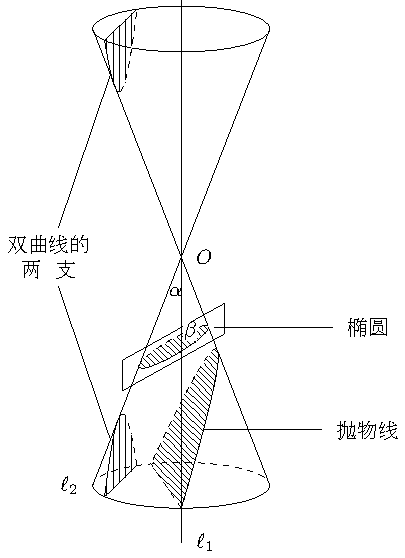
\includegraphics{2-conic-section-all.pdf}
    \caption{}
    \end{minipage}
\end{figure}

设$P$是椭圆截痕上任一点,则过$P$点与轴线平行的直线
全在柱面上,设它交圆$C_1$和圆$C_2$于$Q_1$和$Q_2$两点,则
\begin{itemize}
    \item $PQ_1$和$PF_1$是$P$点到上球的两条切线,所以等长.
    \item   $PQ_2$和$PF_2$是$P$点到下球的两条切线,所以等长.
\end{itemize}

所以,$PF_1+PF_2=PQ_1+PQ_2=Q_1Q_2$

我们让$P$点在椭圆上
变动,则$Q_1Q_2$的变化只
是绕轴旋转,而其长度保持不变的.这就是说,
$PF_1+PF_2=Q_1Q_2=$常数.

$F_1$、$F_2$椭圆焦点,这
就发现了椭圆的特性:椭
圆是平面上一个动点到两个定点$F_1$和$F_2$的距离之
和等于定长的轨迹,$F_1$和
$F_2$叫做椭圆的焦点.

\subsection{圆锥与圆锥曲线}

设$\ell_1$、$\ell_2$是相交于$O$点的两条直线,让$\ell_2$以$\ell_1$为旋转
所得的曲面就是一个圆锥面.再用不过$O$点的平面去截割圆
锥面,所得的曲线叫圆锥曲线,如图2.82所示.设$\ell_1$、$\ell_2$的夹角
为$\alpha$, 截平面和轴的交角为$\beta$, 则不难发现$\beta>\alpha$时,截痕为
椭圆;$\beta=\alpha$时,截痕为抛物线;$\beta<\alpha$时,截痕分为上、下
两支,是双曲线.这三类曲线统称圆锥曲线(或圆锥截线).
这样就对上述这三种曲线有了一种统一的产生办法和处理方
式.

\subsection{圆锥曲线的性质}
在一中前面我们用平面斜截圆柱面而得椭圆这一类型的曲
线,并且利用上、下切球和定点到球面的切线长相等来推导
它的性质:
$PF_1+PF_2=$定长.

在二中我们改用平面来截割圆锥面来构造三种曲线,
其中$\beta>\alpha$时,我们说所得曲线
还是椭圆,这一点还得加以证
明.现在我们把一中的证明略作
修改,证明如下:

我们依然可以作一个
上切球,它和圆锥面相切于圆
$C_1$, 和截割平面相切于$F_1$点,
也可以作一个下切球,它和圆锥
面相切于圆$C_2$, 和截割平面相切
于$F_2$点(唯一不同之点是:
在柱面的情形,上下切球大小相
同,这里的上、下切球一小,一
大.如图2.83).

设$P$为截痕上任意一点,连结直线$OP$, 交$C_1$、$C_2$于$Q_1$
和$Q_2$两点,则同样有
\[PQ_1=PF_1,\qquad PQ_2=PF_2\]
所以$PF_1+PF_2=Q_1Q_2$.

再者,当$P$点在截痕上变动时,$Q_1Q_2$的变化只在锥面上
旋转,而长度不变.这就证明了圆锥的这种截痕($\beta>\alpha$)
满足一中所证的椭圆的性质,因此它也是椭圆.

\begin{figure}[htp]\centering
    \begin{minipage}[t]{0.48\textwidth}
    \centering
    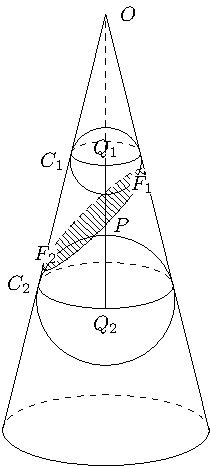
\includegraphics{2-conic-section-ellipse.pdf}
    \caption{}
    \end{minipage}
    \begin{minipage}[t]{0.48\textwidth}
    \centering
    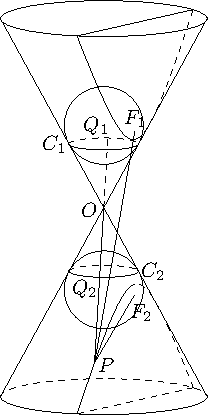
\includegraphics{2-conic-section-hyperbola.pdf}
    \caption{}
    \end{minipage}
    \end{figure}

\subsubsection{双曲线的性质}
设$\beta<\alpha$, 则截割平面交圆锥于上、下两支,如图2.84所
示,我们也可以作上、下两个切球(这次它们分居于圆锥的
上、下两部),它们和圆锥分别切于圆$C_1$和圆$C_2$, 和截平面
相切于$F_1$和$F_2$点.

设$P$为截痕上的任一点,连结直线$OP$, 分别交$C_1$、$C_2$
于$Q_1$和$Q_2$点,则同样地可以得出:
\[PF_1=PQ_1,\qquad PF_2=PQ_2\]
而$QQ_2$的长度是与$P$点位置无关的一个常数,
所以,$Q_1Q_2=PQ_1-PQ_2=PF_1-PF_2=$常数.

这就证明了双曲线的性质:双曲线上的任一点和双曲线
所在平面上两个定点的距离之差等于一个常数.
即
\[PF_1-PF_2=\text{常数}\qquad \text{或}\qquad PF_2-PF_1=\text{常数}\]


\subsubsection{抛物线的性质}
设$\beta=\alpha$, 则截割平面和圆锥交于开口的一支,这时我
们只能作一个球,它和圆锥相交于$C$, 和截平面相切于$F$点.

再者,圆$C$所在的平面和截平面相交于一条直线叫作
准线,如图2.85所示\footnote{原课本插图中$P'Q'$为圆锥左侧母线,这不准确. 为使$P'Q'$与$PR$平行, $P'Q'$在底面上的投影须与抛物线截线正交, 故$P'Q'$不能为图示的左母线. 这已在新插图中订正.}.
\begin{figure}[ht]
    \centering
    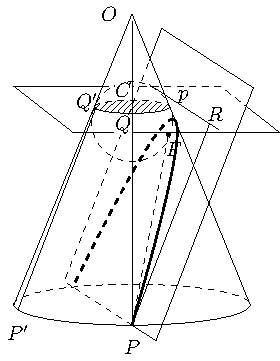
\includegraphics{2-conic-section-parabola.pdf}
    \caption{}
\end{figure}

设$P$是截痕上任一点,连结$PO$交圆$C$于$Q$点,再由$P$点
向准线$p$作垂线$PR$. 由假设,我们可以将$PQ$旋转到和$PR$
平行的位置$P'Q'$, 这样,就不难看出:
\begin{itemize}
    \item $PF=PQ$(切线长相等)
    \item $PQ=P'Q'$(移形公理)
    \item $PR=P'Q'$(平行平面间的平行线段相等)
\end{itemize}

所以$PF=PR=P$点到准线的距离.

总结上面的讨论得到抛物线的性质:
抛物线上任意一点和抛物线所在平面上的一定点和一定
直线的距离相等.即:$PF=PR$.

定点叫作抛物线的焦点,定直线叫做它的准线.


  \chapter{向量与向量运算}
在常用的数量问题中,我们用数去表达各种量,如重
量、长度、面积、体积、密度等等;用加、减、乘、除运算
的组合去表达各种量之间的关系(通称代数通性).在代数
中,我们已掌握了数系的基本性质(即交换律、结合律和分
配律).并熟知了代数学的基本精神在于有效地运用数系
通性,对于各种类型的代数问题谋求通解(即以通性求通
解).现在我们要着手把几何学的讨论也推进到定量的层
面,设法把空间结构有系统地代数化,数量化,这也就是本
章所要详加讨论的课题——\textbf{向量与向量运算}.为了便于同学
们逐步地理解向量这个基本概念,本章的前三节先对平面向
量详加分析,然后再在第四节讨论空间向量.

\section{平面位移向量及其加法运算}

\subsection{位移向量}

如图3.1所示,我们在$\overline{AB}$的端点$B$处画	
上一个箭头表示 线段$\overline{AB}$具有射线$AB$的方向,这种用箭头指明方向的线段叫做\textbf{有向线段},记作$\Vec{AB}$,读作有向线段$AB$,并称A为$\Vec{AB}$的\textbf{始点},$B$为$\Vec{AB}$的\textbf{终点}.$\overline{AB}$的长叫做$\Vec{AB}$的长,并记作$|\Vec{AB}|$.

$\Vec{AB}$和$\Vec{CD}$同向且等长,那么我们称$\Vec{AB}$和$\Vec{CD}$\textbf{相等},记作$\Vec{AB}=\Vec{CD}$(图3.2).

\begin{figure}[htp]\centering
    \begin{minipage}[t]{0.48\textwidth}
    \centering
\begin{tikzpicture}[>=latex, scale=.8]
    \draw[->](0,0)node[below]{$A$}--(2,3)node[above]{$B$};
    \end{tikzpicture}
    \caption{}
    \end{minipage}
    \begin{minipage}[t]{0.48\textwidth}
    \centering
    \begin{tikzpicture}[>=latex, scale=.8]
        \draw[->](0,0)node[below]{$A$}--(2,3)node[above]{$B$};
        \draw [dashed](0,0)--(3,.5);\draw [dashed](2,3)--(5,3.5);
        \draw[->](3,.5)node[below]{$C$}--(5,3.5)node[above]{$D$};
    \end{tikzpicture}
    \caption{}
    \end{minipage}
    \end{figure}

已知方向$ON$(图3.3), 如果平面上的每一点都沿射线
$ON$的方向移动相同的距离,那
么我们称这种平面上全体点的移
动叫做平面上全体点的一个\textbf{平移}.

\begin{figure}[htp]\centering
    \begin{minipage}[t]{0.48\textwidth}
    \centering
\begin{tikzpicture}[>=latex, xscale=.8]
       \draw[->] (0,0)node[right]{$O$}--(0,1)node[right]{$N$};
       \draw[dashed](0,1)--(0,2.5);
\draw[->] (1,0)node[right]{$P$}--(1,2)node[right]{$P_1$};
\draw[->] (2,1)--(2,3);  \draw[->] (3,.5)--(3,2.5);  
\draw[->] (4,1)--(4,3);  \draw[->] (5,.5)--(5,2.5);  
    \end{tikzpicture}
    \caption{}
    \end{minipage}
    \begin{minipage}[t]{0.48\textwidth}
    \centering
    \begin{tikzpicture}[>=latex, scale=1]
        \draw[->] (0,0)node[right]{$P_1$}--(1.5,2)node[right]{$T(P_1)$};
        \draw[->] (2,0)node[right]{$P_2$}--(3.5,2)node[right]{$T(P_2)$};
    \end{tikzpicture}
    \caption{}
    \end{minipage}
    \end{figure}

平面上全体点的一个平移通
常用字母$T$来表示,不同的平移可分别用$T_1,T_2,\ldots$来表示.
如果$P$点通过平移$T$移动到$P_1$点,则$P_1$点叫做$P$点的\textbf{象
点},记作$P_1=T(P)$, 这时有向线段$\Vec{PP_1}$; 可写作$\Vec{PT(P)}$.

为了给出一个平移,根据定义,只需给出平面上任一点
和它的象点即可.设$P_1=T(P)$, 则$P$、$P_1$这两点 就完全
确定了平移$T$的方向和距离;对平面上任一点$A$, 我们都
可作$\Vec{AA_1}=\Vec{PP_1}$, 这样$A$的象点$A_1$也就被$\Vec{PP_1}$所唯一确
定,这也就是说,给定了一个平移$T$, 如果$P_1=T(P)$, 那
么这个平移$T$完全被$\Vec{PT(P)}$所唯一确定,通常我们就用
$\Vec{PT(P)}$或$\Vec{PP_1}$表示这个平移.

显然,平面上全体点的一个移动是一个平移的充要条件
是:对平面上任意两点$P_1$、$P_2$,都有
\[\Vec{P_1T(P_1)}=\Vec{P_2T(P_2)}\]

从以上讨论知,一个平移$T$只有两个要素:\textbf{方向和距离},
因此平面上的一个平移$T$, 可用
那些同向且等长的任一条有向线段来表示.

几次连续平移的结果,叫做平移的\textbf{合成}.设$T_1$、$T_2$是
两次连续平移,这两次连续平移的合成通常记作$T_2\circ T_1$(第
一次平移写在右边),类似地$T_3\circ T_2\circ T_1$, 表示$T_1$、$T_2$、$T_3$三
次连续平移的合成.

\begin{blk}{定理}
    平移的合成还是一个平移且平移的合成满足交换
律.
\end{blk}

\begin{proof}
设$T_1$、$T_2$是两个平移,我们要证明的是:$T_2\circ T_1$也是一个平移,$T_2\circ T_1=T_1\circ T_2$.

设$P$、$Q$是平面上任意两点(图3.5),$P_1=T_1(P)$、
$P_2=T_2(P_1)$、$Q_1=T_1(Q)$、$Q_2=T_2(Q_1)$, 则$P_2=T_2(T_1(P))$, $Q_2=T_2(T_1(Q))$
\begin{figure}[htp]
    \centering
\begin{tikzpicture}[>=latex]
\tkzDefPoints{0/0/P, .85/2/P_1, 2/3/P_2, 4/0/Q}
\tkzDefPointsBy[translation= from P to Q](P_1,P_2){Q_1,Q_2}
\draw[->](P) -- node[left]{$T_1$} (P_1);
\draw[->](Q) -- node[left]{$T_1$} (Q_1);
\draw[->](P) --  (P_2);
\draw[->](Q) -- (Q_2);
\draw[->](P_1) -- node[left]{$T_2$} (P_2);
\draw[->](Q_1) -- node[left]{$T_2$} (Q_2);
\tkzDrawSegments(P,Q P_2,Q_2 P_1,Q_1)
\tkzLabelPoints[left](P_2,Q_2,P_1,Q_1)
\tkzLabelPoints[below](P,Q)
\end{tikzpicture}
    \caption{}
\end{figure}

我们要证明$T_2\circ T_1$是一个平移也就是要证
明$\overline{PP_2}$与$\overline{QQ_2}$平行且等
长.即
\[\Vec{PP_2}=\Vec{QQ_2}\]
由于$T_1$、$T_2$都是平移,则
\[\Vec{PP_1}=\Vec{QQ_1},\qquad \Vec{P_1P_2}=\Vec{Q_1Q_2}\]
连$P$、$P_2$, $Q$、$Q_2$由平行四边形基本定理(即\textbf{一个四边形的
一组对边平行且等长,则另一组对边也平行且等长}),容易
证明:
\[\Vec{PP_2}=\Vec{QQ_2}\]
这就证明了$T_2\circ T_1$也是一个平移.



设点$P$是平面上任一点,$P_1=T_1(P)$, $P_2=T_2(P_1)$,
则$P_2=T_2(T_1(P))$, 这就是说$T_2\circ T_1$把$P$点移动到$P_2$点.

设$Q=T_2(P)$, 由平移定义可知
\[\Vec{P_1P_2}=\Vec{PQ}\]
又由上述平行四边形基本定理可证
\[\Vec{PP_1}=\Vec{QP_2}\]
这就是说
\[P_2=T_1(Q)=T_1(T_2(P))\]
所以
\[T_2\circ T_1=T_1\circ T_2\]
\end{proof}

\begin{figure}[htp]\centering
    \begin{minipage}[t]{0.48\textwidth}
    \centering
\begin{tikzpicture}[>=latex, scale=1]
    \draw[->](0,0)node[below]{$P$}--node[below]{$T_2$}(3,0) node[below]{$Q$} ;
    \draw[->](0,0)--node[left]{$T_1$}(1,2)node[above]{$P_1$}  ;
    \draw[->](3,0)--node[right]{$T_1$}(4,2)node[above]{$P_2$};
    \draw[->>, thick](0,0)--node[above=1pt, rotate=30]{$T_2\circ T_1$}(4,2)  ;
    \draw[->](1,2)--node[above]{$T_2$}(4,2)  ;
    \end{tikzpicture}
    \caption{}
    \end{minipage}
    \begin{minipage}[t]{0.48\textwidth}
    \centering
    \begin{tikzpicture}[>=latex, scale=.8]
        \draw[->](0,0)--node[below]{$T_1$}(4,0);
        \draw[->](0,0)--node[left]{$T_2$}(0,4);
        \draw[->>](0,0)--node[above, rotate=45]{$5\sqrt{2}$}(4,4);
        \draw[->](4,0)--node[right]{$T_2$}(4,4);
        \draw[->](0,4)--node[above]{$T_1$}(4,4);

        \draw[->](-1,2)--(-1,3)node[left]{北};
    \end{tikzpicture}
    \caption{}
    \end{minipage}
    \end{figure}


\begin{example}
    已知$T_1$表示平移“向东5公里”,$T_2$表示平移
“向北5公里”,求$T_1\circ T_2$, $T_2\circ T_1$.
\end{example}

\begin{solution}
    $T_1\circ T_2=T_2\circ T_1$都表示平移:“向东北$5\sqrt{2}$公里”(图3.7)
\end{solution}

\begin{example}
    已知:$T_1:$ “向东5公里”,$T_2:$ “向西10公里”,求$T_1\circ T_2$和$T_2\circ T_1$.
\end{example}

\begin{solution}
   $T_1\circ T_2=T_2\circ T_1$都表示平移:“向西5公里”(图3.8).
\end{solution}

\begin{example}
    已知$T_1:$ “向东3公里”,$T_2:$ “向西3公里”,
求$T_1\circ T_2$, $T_2\circ T_1$.
\end{example}

\begin{solution}
    $T_1\circ T_2=T_2\circ T_1$都表示“原地不动”(图3.9).
这种原地不动的“移动”,可看作平移的特例,叫做\textbf{零平移},零平移记作$\Vec{0}$.
\end{solution}

\begin{blk}
    {定义} 平面上全体点的一个平移,叫做平面上的一个位
移向量,简称向量.
\end{blk}

\begin{figure}[htp]\centering
    \begin{minipage}[t]{0.48\textwidth}
    \centering
\begin{tikzpicture}[>=latex, scale=.9]
\draw[very thick, <->] (2,0)--node[above]{$T_1$}(0,0)--(-2,0);
\draw[thick, ->]  (-4,0)--node[below]{$T_1$}(-2,0);
\draw[thick, ->](-4,0)--(-4,1)node[above]{北};
\draw(0,0)[fill=black]circle (1.5pt);
\draw[thick, ->](2,-.25)--node[below]{$T_2$}(-2,-.25);
\draw[thick, ->](0,.25)--node[above]{$T_2$}(-4,.25);
\draw(-4,0)--(2.5,0);
    \end{tikzpicture}
    \caption{}
    \end{minipage}
    \begin{minipage}[t]{0.48\textwidth}
    \centering
    \begin{tikzpicture}[>=latex, scale=.9]
\draw[very thick, <->] (2,0)--node[above]{$T_1$}(0,0)--node[below]{$T_2$}(-2,0);
\draw[thick, ->](2,-.25)--node[below]{$T_2$}(0,-.25);
\draw[thick, ->](-2,.25)--node[above]{$T_1$}(0,.25);
\draw(0,0)[fill=black]circle (1.5pt);
\draw(-2.5,0)--(2.5,0);
    \end{tikzpicture}
    \caption{}
    \end{minipage}
    \end{figure}

如果我们用$\Vec{AB}$, $\Vec{CD}$表示平面上点的平移,我们就说向量$\Vec{AB},\Vec{CD},\ldots$.印刷时
经常用粗体字$\bf{a}$、$\bf{b}$、$\bf{c}$等表
示一个向量.向量$\bf{a}$、$\bf{b}$、$\bf{c}$在
手写时常写作$\vec{a}$、$\vec{b}$、$\vec{c}$.

如果向量$\vec{a}$, 把$A$点移
动到$B$点,$C$点移动到$D$点,$E$点移动到$F$点(图3.10),则
\[\vec{a}=\Vec{AB}=\Vec{CD}=\Vec{EF}=\cdots\]
这些同向且等长的有向线段都表示同一个向量,也就是说它
们中的任一个都可用来表示向量$\vec{a}$.
\begin{figure}[htp]
    \centering
    \begin{tikzpicture}[>=latex]
\draw[thick, ->](0,0)node[below]{$A$}--node[left]{$\vec{a}$}(1.5,3)node[above]{$B$};
\draw[thick, ->](1,0.25)node[below]{$C$}--node[left]{$\vec{a}$}(2.5,3.25)node[above]{$D$};
\draw[thick, ->](2,.5)node[below]{$E$}--node[left]{$\vec{a}$}(3.5,3+.5)node[above]{$F$};
\draw[thick, ->](3,.75)--node[left]{$\vec{a}$}(4.5,3+.75);        
    \end{tikzpicture}

    \caption{}
\end{figure}


若$\vec{a}=\Vec{AB}$, 则$\Vec{AB}$的长叫做$\vec{a}$的长度,记作$|\Vec{AB}|$或$|\vec{a}|$.
射线$\Vec{AB}$的方向叫做向量$\vec{a}$的方向.零平移又叫做\textbf{零向量},它
的方向不确定.

如果$\Vec{AB}$与$\Vec{CD}$的方向相同,那么$\Vec{AB}$, $\Vec{CD}$叫做\textbf{同向
向量},如果$\Vec{A_1B_1}$、$\Vec{C_1D_1}$的方向相反,那么$\Vec{A_1B_1}$、$\Vec{C_1D_1}$叫
做\textbf{反向向量}(图3.11).方向相同或相反的向量,叫做\textbf{平行
向量}.
\begin{figure}[htp]
    \centering
\begin{tikzpicture}[>=latex]
\begin{scope}
    \draw[thick, ->] (0,0)node[below]{$A$}--(0,3)node[above]{$B$};
    \draw[thick, ->] (1,.5)node[below]{$C$}--(1,2.5)node[above]{$D$};    
    \draw[thick, ->] (2,1)--node[left]{$\vec{a}$}(2,3);
\end{scope}
\begin{scope}[xshift=5cm]
    \draw[thick, ->] (0,0)node[below]{$A_1$}--(0,3)node[above]{$B_1$};
    \draw[thick, <-] (1,.5)node[below]{$D_1$}--(1,3)node[above]{$C_1$};    
    \draw[thick, <-] (2,1)--node[left]{$\vec{b}$}(2,2.5);
\end{scope}
\end{tikzpicture}
    \caption{}
\end{figure}

长度为1个单位的向量叫做\textbf{单位向量},通常我们用单位
向量表示平面上的一个方向.

以后我们用到记号$\Vec{AB}$或$\vec{a}$, 它们表示的是一个有向线段
还是一个向量,一般我们都不另加说明,读者可根据实际问
题加以区分.

\begin{ex}
\begin{enumerate}
    \item 用有向线段表示以下平移:
\begin{enumerate}
    \item $T_1$: 向东5cm;
    \item $T_2$: 向南偏西$30^{\circ}$, 3cm;
    \item $T_3$: 向北偏西$60^{\circ}$, 50km.
\end{enumerate}
\item  用有向线段表示以下两个平移的合成:
\begin{enumerate}
    \item $T_1$: 向西5里,$T_2$: 向南3里.
    \item $T_1$: 向北4里,$T_2$: 向西8里.
\end{enumerate}
\end{enumerate}
\end{ex}

\subsection{向量的加法与减法}
向量$\vec{a}$与$\vec{b}$的合成就叫做$\vec{a}$与
$\vec{b}$的和,记作$\vec{a}+\vec{b}$, 即
\[\vec{a}+\vec{b}=\vec{b}\circ \vec{a}\]

由上节定理可知,$\vec{a}$与$\vec{b}$的和$\vec{a}+\vec{b}$也是一个向量.由
于每个向量可由一点和它的象点所唯一确定,所以可按下面
方法作$\vec{a}+\vec{b}$.

在平面上,任取一点$A$ (图3.12), 作$\Vec{AB}=\vec{a}$, $\Vec{BC}=\vec{b}$, 即
$\vec{a}$与$\vec{b}$的合成把$A$点移动到$C$点,因而
\[\Vec{AC}=\vec{a}+\vec{b}\]
\begin{figure}[htp]
    \centering
\begin{tikzpicture}[>=latex, scale=1.5]
\begin{scope}
    \draw[->,  thick](0,0)--node[left]{$\vec{a}$}(1,1);
    \draw[->,  thick] (1,.5)--node[above]{$\vec{b}$}(2.5,.6);
\end{scope}

\begin{scope}[xshift=3.5cm]
    \draw[->,  thick](0,0)node[below]{$A$}--node[left]{$\vec{a}$}(1,1);
    \draw[->,  thick](1,1)--node[above]{$\vec{b}$}(2.5,1.1)node[right]{$C$};
    \draw[->,  thick](0,0)--node[right]{$\vec{a}+\vec{b}$}(2.5,1.1);
\end{scope}
\end{tikzpicture}    
    \caption{}
\end{figure}

以上求和作图法叫做\textbf{三角形求和法则}.

由于平移的合成满足交换律,所以向量加法也满足交换
律,即
\[\vec{a}+\vec{b}=\vec{b}+\vec{a}\]

读者不难从图3.13
去验证,向量加法还满
足结合律,即
\[(\vec{a}+\vec{b})+\vec{c}=\vec{a}+(\vec{b}+\vec{c})\]
\begin{figure}[htp]\centering
    \begin{minipage}[t]{0.48\textwidth}
    \centering
\begin{tikzpicture}[>=latex,scale=1.5]
    \tkzDefPoints{0/0/A, 1/1.5/B, 3/1.7/C, 3.5/0/D}
\draw[->, thick](A)--node[left]{$\vec{a}$}(B);
\draw[->, thick](A)--node[above,rotate=30]{$\vec{a}+\vec{b}$}(C);
\draw[->, thick](A)--node[below]{$(\vec{a}+\vec{b})+\vec{c}=\vec{a}+(\vec{b}+\vec{c})$}(D);
\draw[->, thick](B)--node[above]{$\vec{b}$}(C);
\draw[->, thick](B)--node[above,rotate=-35]{$\vec{b}+\vec{c}$}(D);
\draw[->, thick](C)--node[right]{$\vec{c}$}(D);
    \end{tikzpicture}
    \caption{}
    \end{minipage}
    \begin{minipage}[t]{0.48\textwidth}
    \centering
    \begin{tikzpicture}[>=latex, scale=1.5]
      \draw[->, thick](0,0)--node[left]{$\vec{a}$}(1,1.5);
      \draw[<-, thick](1.25,0)--node[left]{$\vec{x}$}node[right]{$-\vec{a}$}(2.25,1.5);
    \end{tikzpicture}
    \caption{}
    \end{minipage}
    \end{figure}

容易看出,$\vec{a}+\vec{0}=\vec{0}+\vec{a}=\vec{a}$.

如果向量$\vec{a}$与$\vec{x}$反向且等长,那么由求和作图法可知
(图3.14)
\[\vec{a}+\vec{x}=\vec{0}\]

如果用$-\vec{a}$表示$\vec{x}$, 那么$-\vec{a}$叫
做$\vec{a}$的\textbf{逆向量}或\textbf{负向量},于是
\[\vec{a}+(-\vec{a})=\vec{0}\]
如图3.15所示.

\begin{figure}[htp]
    \centering
    \begin{minipage}[t]{0.48\textwidth}
    \centering
    \begin{tikzpicture}[>=latex, scale=1.4]
\tkzDefPoints{0/0/A, 3/0/B, 1.4/1.5/C, 0/1/A', 3.5/1/B'}
\tkzDefPointsBy[translation = from A to A'](C){C'}
\tkzDefPointsBy[translation = from B to B'](C){C''}
\draw[->, thick](A)--node[below]{$\vec{a}+(-\vec{b})$}(B);
\draw[->, thick](A)--node[left]{$\vec{a}$}(C);
\draw[->, thick](A')--node[left]{$\vec{a}$}(C');
\draw[<-, thick](B)--node[right]{$-\vec{b}$}(C);
\draw[->, thick](B')--node[right]{$\vec{b}$}(C'');

    \end{tikzpicture}
    \caption{}
    \end{minipage}
    \begin{minipage}[t]{0.48\textwidth}
    \centering
    \begin{tikzpicture}[>=latex, scale=1.4]
\tkzDefPoints{0/0/A, 3/0/B, 3.7/2/C}
\tkzDefPointsBy[translation = from B to C](A){D}
\tkzDrawSegments[->](D,C B,C D,B)
\tkzDrawSegments(A,C)
\tkzInterLL(A,C)(B,D)  \tkzGetPoint{O}
\draw(A)--node[above]{$\vec{a}+\vec{b}$}(O);
\draw(O)--node[above]{$\vec{a}-\vec{b}$}(B);

\draw[->](A)--node[below]{$\vec{a}$}(B);
\draw[->](A)--node[left]{$\vec{b}$}(D);
\tkzLabelPoints[below](A,B)
\tkzLabelPoints[above](C,D)

    \end{tikzpicture}
    \caption{}
    \end{minipage}
  \end{figure}

\begin{example}
已知:$\parallelogram ABCD$, $\Vec{AB}=\vec{a}$,$\Vec{AD}=\vec{b}$(图3.16).

求证:$\Vec{AC}=\vec{a}+\vec{b},\qquad \Vec{DB}=\vec{a}-\vec{b}$
\end{example}

\begin{proof}
因为$\Vec{AC}=\Vec{AB}+\Vec{BC},\; \Vec{BC}=\Vec{AD}$,所以
\[\Vec{AC}=\Vec{AB}+\Vec{AD}=\vec{a}+\vec{b}\]
又因为$\Vec{DB}=\Vec{DC}+\Vec{CB},\quad \Vec{DC}=\vec{a},\quad \Vec{CB}=-\vec{b}$

所以$\Vec{DB}=\vec{a}-\vec{b}$
\end{proof}    

由例3.4可知,位于一个平行四边形的一条“对角线向量”等于相邻两个“边向量”之和,而另一条“对角线向量”等于相邻两个“边向量”之差,由此,我们还可得到求两个向量和与差的方法如下:

\begin{blk}
   {求和的平行四边形法则} 已知$\vec{a}$、$\vec{b}$, 任取一点$A$, 作$\Vec{AB}=\vec{a}$, $\Vec{AD}=\vec{b}$, 再以$\Vec{AB}$、$\Vec{AD}$为边作$\parallelogram ABCD$, 则对角线上的向量$\Vec{AC}$就是$\vec{a}$与$\vec{b}$之和,即
   \[\vec{a}+\vec{b}=\Vec{AB}+\Vec{AD}=\Vec{AC}\] 
\end{blk}

\begin{blk}
    {求$\vec{a}-\vec{b}$的三角形法则} 已知$\vec{a}$、$\vec{b}$, 在平面上任取一点$A$, 作$\Vec{AB}=\vec{a}$, $\Vec{AD}=\vec{b}$, \textbf{以减量$\vec{b}$的终点($D$)为始点,被减量$\vec{a}$的终点($B$)为终点的向量$\Vec{DB}$就是$\vec{a}-\vec{b}$}, 即
    \[\vec{a}-\vec{b}=\Vec{AB}-\Vec{AD}=\Vec{DB}\] 
\end{blk}

对于多个向量$\vec{a}_1,\vec{a}_2,\ldots,\vec{a}_n$的求和法则,可由三角形求和法则推广如下:

已知$\vec{a}_1,\vec{a}_2,\ldots,\vec{a}_n$,在平面上任取一点$O$, 作$\Vec{OA_1}=\vec{a}_1$, 然后在$A_1$上引$\Vec{A_1A_2}=\vec{a}_2$, 再在$A_2$上引$\Vec{A_2A_3}=\vec{a}_3$, 如此下去,我们由这$n$条向量构成一条折线,由两个向量的求和
法则,我们可推知,以第一条有向线段的始点为始点,最后一条有向线段的终点为终点的有向线段所表示的向量就是这
$n$个向量之和,在图3.17中,
\[\vec{a}_1+\vec{a}_2+\vec{a}_3+\vec{a}_4=\Vec{OA_1}+\Vec{A_1A_2}+\Vec{A_2A_3}+\Vec{A_3A_4}=\Vec{OA_4}\]

\begin{figure}[htp]
    \centering
    \begin{minipage}[t]{0.48\textwidth}
    \centering
    \begin{tikzpicture}[>=latex, scale=1.5]
\tkzDefPoints{0/0/O, .5/1/A_1, 1.5/1.5/A_2, 2.5/1/A_3, 3/0/A_4}
\draw[->, thick](O)--node[left]{$\vec{a}_1$}(A_1);
\draw[->, thick](O)--node[below]{$\vec{a}_1+\vec{a}_2+\vec{a}_3+\vec{a}_4$}(A_4);
\draw[->, thick](A_1)--node[above]{$\vec{a}_2$}(A_2);
\draw[->, thick](A_2)--node[above]{$\vec{a}_3$}(A_3);
\draw[->, thick](A_3)--node[right]{$\vec{a}_4$}(A_4);
    \end{tikzpicture}
    \caption{}
    \end{minipage}
    \begin{minipage}[t]{0.48\textwidth}
    \centering
    \begin{tikzpicture}[>=latex, scale=.7]
\draw(-2,0)--(5,0);
\draw[->](0,-4.5)--(0,3)node[left]{北};
\draw[->, thick](0,0)--node[below]{$\vec{a}$}(2,0)node[below]{$A$};
\draw[->, thick](0,0)--node[above]{$\vec{b}$}(-1,0)node[below]{$B$};
\node at (0,0)[below left]{$O$};
\draw[->, thick](2,0)--node[below]{$\vec{a}$}(4,0)node[below]{$E$};
\draw[->, thick](0,0)--(0,2)node[left]{$C$};
\draw[->, thick](0,-2)--node[right]{$\vec{d}$}(0,-4)node[left]{$D$};
\draw[->, thick](0,0)--(0,-2)node[left]{$H$};
\draw[->, thick](0,0)--(1,0)node[above]{$F$};
\draw[->, thick](0,0)--(2,2)node[above]{$G$};
\draw[->, thick](2,0)--node[right]{$\vec{c}$}(2,2);


    \end{tikzpicture}
    \caption{}
    \end{minipage}
  \end{figure}

\begin{example}
已知:$\vec{a}=$“向东10km”,$\vec{b}=$“向西5km”,$\vec{c}=$“向北10km”,$\vec{d}=$“向南20km”,求:$\vec{a}+\vec{a}$, $\vec{a}+\vec{b}$, $\vec{a}+\vec{c}$, $\vec{c}+\vec{d}$.
\end{example}

\begin{solution}
如图3.18所示,作$\Vec{OA}=\vec{a}$, $\Vec{OB}=\vec{b}$, $\Vec{OC}=\vec{c}$, $\Vec{OD}=\vec{d}$,则:
\[\begin{split}
    \Vec{OE}&=\vec{a}+\vec{a}=\text{“向东20km”}\\
    \Vec{OF}&=\vec{a}+\vec{b}=\text{“向东5km”}\\
    \Vec{OG}&=\vec{a}+\vec{c}=\text{“向东北$10\sqrt{2}$km”}\\
    \Vec{OH}&=\vec{c}+\vec{d}=\text{“向南10km”}   
\end{split}\]
\end{solution}

由例3.5, 我们可以看出,两个方向相同的向量相加时,它们的和向量的方向与已知两个向量的方向相同,其长度等于它们的长度之和,两个方向相反的向量相加时,它们的和向量的方向与长度较长的那个向量方向相同,其长度等于两个向量长度差的绝对值.  

\subsubsection*{练习}

\begin{enumerate}
    \item 作出下列各组向量的和:
\begin{figure}[htp]
  \centering
  \begin{tikzpicture}[>=latex]
\begin{scope}[scale=.8]
\draw[<->, thick](3,2.2)--node[above]{$\vec{b}$}(0,0)--node[below]{$\vec{a}$}(-2,2);    
\end{scope}
\begin{scope}[xshift=5cm, scale=.8]
    \draw[->, thick](0,3)--node[left]{$\vec{a}$}(0,1);
\draw[->, thick](0,1)--node[below]{$\vec{b}$}(2.5,1);
\end{scope}
\begin{scope}[yshift=-3cm, xshift=-2cm]
      \draw[->, thick](0,1)--node[above]{$\vec{a}$}(2.5,1.5);
\draw[<-, thick](0,0)--node[above]{$\vec{b}$}(2,-.5);
\end{scope}
\begin{scope}[xshift=1.5cm, yshift=-3cm]
 \draw[->, thick](0,2)--node[right]{$\vec{b}$}(2.5,0);
\draw[<-, thick](-0.2,0)--node[left]{$\vec{a}$}(2,2);    
\end{scope}
\begin{scope}[xshift=5cm, yshift=-3cm]
    \draw[->, thick](0,.7)--node[above]{$\vec{a}$}(1.5,.7);
\draw[->, thick](0,0)--node[below]{$\vec{b}$}(2.5,0);      
\end{scope}
\begin{scope}[xshift=1cm, yshift=-6cm]
    \draw[<->, thick](-2.5,0)--node[above]{$\vec{b}$}(0,0)--node[above]{$\vec{a}$}(2,0);
  \tkzDrawPoint(0,0)
\end{scope}
\begin{scope}[xshift=4cm, yshift=-6cm]
    \draw[->, thick](0,0)--node[left]{$\vec{a}$}(2,1.8);
  \draw[->, thick](2,1)--node[above right]{$\vec{b}$}(4.5,1);
  \draw[->, thick](2.5,1.5)--node[below left]{$\vec{c}$}(4,-.5);
\end{scope}
  \end{tikzpicture}
\end{figure}

\item 求$\vec{a}-\vec{b}$
\begin{figure}[htp]
    \centering
    \begin{minipage}[t]{0.48\textwidth}
    \centering
    \begin{tikzpicture}[>=latex, scale=1.4]
\draw[<->, thick](1,1.2)node[right]{$A$}--node[above]{$\vec{a}$}(0,0)--node[below]{$\vec{b}$}(2,0)node[right]{$B$};
  \end{tikzpicture}
  \caption*{(1)}
    \end{minipage}
    \begin{minipage}[t]{0.48\textwidth}
    \centering
    \begin{tikzpicture}[>=latex, scale=1.5]
\draw[<->, thick](.5,1.2)node[right]{$B$}--node[above]{$\vec{b}$}(0,0)--node[below]{$\vec{a}$}(2,0.25)node[right]{$A$};  
    \end{tikzpicture}
    \caption*{(2)}
    \end{minipage}
  \end{figure}

  \begin{figure}[htp]
    \centering
    \begin{minipage}[t]{0.48\textwidth}
    \centering
    \begin{tikzpicture}[>=latex, scale=1]
  \draw[->, thick](0,0)--node[above]{$\vec{b}$}(4,0);
  \draw[->, thick](0.5,-.5)--node[above]{$\vec{a}$}(1.5,2);
    \end{tikzpicture}
    \caption*{(3)}
    \end{minipage}
    \begin{minipage}[t]{0.48\textwidth}
    \centering
    \begin{tikzpicture}[>=latex, scale=1]
        \draw[<->, thick](-2,0)--node[above]{$\vec{a}$}(0,0)--node[above]{$\vec{b}$}(2.5,0);
        \tkzDrawPoint(0,0)
    \end{tikzpicture}
    \caption*{(4)}
    \end{minipage}
  \end{figure}


    \item 任给两个向量$\vec{a}$、$\vec{b}$,用平行四边形法则求$\vec{a}+\vec{b}$.
    \item 已知$\triangle ABC$, 求证:$\Vec{AB}+\Vec{BC}+\Vec{CA}=0$.
    \item 如果三个向量$\vec{a}$、$\vec{b}$、$\vec{c}$, 满足$\vec{a}+\vec{b}+\vec{c}=0$, 问表示这三个向量的有向线段能否构成三角形.

\end{enumerate}

\subsection{$n$个$\vec{a}$连加之和}

\begin{blk}{定义}
如果$n$是正整数,定义
\[\underbrace{\vec{a}+\vec{a}+\vec{a}+\cdots+\vec{a}}_{\text{$n$个}}=n\vec{a}\] 
\end{blk}

例如,$\vec{a}+\vec{a}+\vec{a}+\vec{a}=4\vec{a}$.

\begin{example}
如$n,m$为正整数,试证:
\begin{enumerate}
    \item $n\left(m\vec{a}\right)=(mn)\vec{a}$
    \item $n\left(\vec{a}+\vec{b}\right)=n\vec{a}+n\vec{b}$(分配律)
\end{enumerate}
\end{example}   

\begin{proof}
\begin{enumerate}
    \item 
\[\begin{split}
     n\left(m\vec{a}\right)&=\overbrace{m\vec{a}+m\vec{a}+\cdots +m\vec{a}}^{n\text{个}}\\
&=\underbrace{\underbrace{\vec{a}+\vec{a}+\cdots+\vec{a}}_{m\text{个}}+\underbrace{\vec{a}+\vec{a}+\cdots+\vec{a}}_{m\text{个}}+\cdots +\underbrace{\vec{a}+\vec{a}+\cdots+\vec{a}}_{m\text{个}}}_{n\text{个}}\\
&=(nm)\vec{a} 
\end{split}\]
\item 
\[\begin{split}
     n\left(\vec{a}+\vec{b}\right)&=\overbrace{\left(\vec{a}+\vec{b}\right)+\left(\vec{a}+\vec{b}\right)+\cdots +\left(\vec{a}+\vec{b}\right)}^{n\text{个}}\\
   &=  \underbrace{\vec{a}+\vec{a}+\cdots+\vec{a}}_{n\text{个}}+\underbrace{\vec{b}+\vec{b}+\cdots+\vec{b}}_{n\text{个}}\\
     &=n\vec{a}+n\vec{b}
\end{split}\]
\end{enumerate}    
\end{proof}

下面让我们来分析一下$n\left(\vec{a}+\vec{b}\right)=n\vec{a}+n\vec{b}$的几何意义:取$\Vec{AB}=\vec{a}$, $\Vec{BC}=\vec{b}$ (图3.19), 则$\vec{a}+\vec{b}=\Vec{AC}$, 再取$\Vec{AB'}=n\vec{a}$, 过$B'$点作$BC$的平行线,取$B'C'$和$\Vec{DC}$同向且其长是$|\Vec{BC}|$的$n$倍,即$\Vec{B'C'}=n\vec{b}$, 由上述分配律有:
\[\Vec{AC'}=\Vec{AB'}+\Vec{B'C'}=n\vec{a}+n\vec{b}=n\left(\vec{a}+\vec{b}\right)=n\Vec{AC}\]
由此可知,$A$、$C$、$C'$三点共线并且$\Vec{AC'}$的长度是$\Vec{AC}$长度的$n$倍.这就证明了相似三角形基本定理(即\textbf{两个三角形中,如果有三个角对应相等,那么它们的三边就对应成比例}).

反之,如果$\triangle ABC\backsim \triangle AB'C'$且
$\frac{\overline{AB'}}{\overline{AB}}=n$,
则由相似三角形定理有
\[\Vec{AB'}=n\Vec{AB},\qquad \Vec{B'C'}=n\Vec{BC},\qquad \Vec{AC'}=n\Vec{AC}\]
\[\begin{split}
    \Vec{AC'}&=n\Vec{AC}=n\left(\Vec{AB}+\Vec{BC}\right)\\
    \Vec{AC'}&=\Vec{AB'}+\Vec{B'C'}=n\Vec{AB}+n\Vec{BC}
\end{split}\]
故得
\[n\left(\Vec{AB}+\Vec{BC}\right)=n\Vec{AB}+n\Vec{BC}\]
这就证明了上述分配律成立.

总结上面的分析,我们可以看到,运算律$n(\vec{a}+\vec{b})=
=n\vec{a}+n\vec{b}$和相似比为整数的相似三角形定理是同一几何事实的两种表达形式,它们在逻辑上具有等价关系.我们还可以把$n(\vec{a}+\vec{b})=
=n\vec{a}+n\vec{b}$的代数证明和边长之比为$n$的相似三角形定理的几何证明再加以分析比较.为清楚起见,我们取$n=3$ (图3.19).

\begin{figure}[htp]
    \centering
    \begin{minipage}[t]{0.58\textwidth}
    \centering
    \begin{tikzpicture}[>=latex, scale=1]
\tkzDefPoints{0/0/A, 5/0/B', 6/3/C'}
\tkzDefPointWith[linear, K=.333](A,C') \tkzGetPoint{C}
\tkzDefPointWith[linear, K=.333](A,B') \tkzGetPoint{B}
\tkzDefPointWith[linear, K=.333](B',C') \tkzGetPoint{D''}
\tkzDefPointWith[linear, K=.667](A,C') \tkzGetPoint{C''}
\tkzDefPointWith[linear, K=.667](A,B') \tkzGetPoint{B''}
\tkzDefPointWith[linear, K=.667](B',C') \tkzGetPoint{D'}
\tkzDrawSegments[thick, ->](A,C A,B A,B' B',C')
\tkzDrawSegments(A,C' C,D'' C'',D' C,B C'',B'')
\tkzDrawSegments[dashed](B,D')
\tkzLabelPoints[below](A,B,B')
\tkzLabelPoints[above](C,C')

\tkzInterLL(B'',C'')(C,D'')  \tkzGetPoint{O}

\draw(A)--node[below]{$\vec{a}$}(B);
\draw(A)--node[above left]{$\vec{a}+\vec{b}$}(C);
\draw(C)--node[above]{$\vec{a}$}(O);
\draw(C'')--node[above]{$\vec{a}$}(D');
\draw(C)--node[right]{$\vec{b}$}(B);
\draw(C'')--node[right]{$\vec{b}$}(O); 
    \end{tikzpicture}
    \caption{}
    \end{minipage}
    \begin{minipage}[t]{0.38\textwidth}
    \centering
    \begin{tikzpicture}[>=latex, scale=1]
\tkzDefPoints{0/0/A, 0/.6/A_1, 0/1.2/A_2, 0/2.4/A_{n-1}, 0/3.3/B}
\tkzDrawSegments[->](A,B)
\tkzLabelPoints[left](A_1,A_2,A_{n-1})
\tkzDrawPoints(A_1,A_2,A_{n-1})
\tkzLabelPoints[below](A)
\tkzLabelPoints[above](B)
    \end{tikzpicture}
    \caption{}
    \end{minipage}
  \end{figure}


\begin{proof}
\textbf{代数证明}
\begin{align*}
3 \left(\vec{a}+\vec{b}\right) &= \left(\vec{a}+\vec{b}\right)+\left(\vec{a}+\vec{b}\right)+\left(\vec{a}+\vec{b}\right)  \tag{用一次交换律}\\
&=\vec{a}+\vec{a}+\vec{b}+\vec{b}+\vec{a}+\vec{b} \tag{用两次交换律}\\
&= \vec{a}+\vec{a}+\vec{a}+\vec{b}+\vec{b}+\vec{b} =3\vec{a}+3\vec{b}
\end{align*}

\textbf{几何证明:}
主要是用平行分割把$\triangle AB'C'$分割成$3^2=9$个和$\triangle ABC$全等的小三角形来证明相似三角形定理(参看第二册第三章).
\end{proof}

比较上述代数证明和几何证明,可以看出,代数证明不需要作辅助线,比较简单明了.有意思的是几何证明中出现了三个平行四边形,应用了三次平行四边形定理,这正好与代数证明中应用了三次交换律相对应.

设$\Vec{AB}=\vec{a}$(图3.20),将$\overline{AB}$等分为$n$段:$\overline{AA_1},\overline{A_1A_2},\overline{A_2A_3},\ldots,\overline{A_{n-1}B}$,则有
\[\Vec{AA_1}=\Vec{A_1A_2}=\Vec{A_2A_3}=\cdots=\Vec{A_{n-1}B}\]
所以
\[n\Vec{AA_1}=\Vec{AA_1}+\Vec{A_1A_2}+\Vec{A_2A_3}+\cdots+\Vec{A_{n-1}B}=\Vec{AB}=\vec{a}\]
我们把上述$\Vec{AA_1}$定义为$\frac{1}{n}\vec{a}$,再者,我们把$\frac{m}{n}\vec{a}$定义为$\frac{1}{n}\left(m\vec{a}\right)$,其性质为
\[n\left(\frac{m}{n}\vec{a}\right)=m\vec{a}\]


\begin{example}
    试证
\begin{enumerate}
    \item $\frac{m}{n}\left(\frac{p}{q}\vec{a}\right)=\left(\frac{m}{n}\frac{p}{q}\right)\vec{a}$
    \item $\frac{n}{m}\left(\vec{a}+\vec{b}\right)=\frac{n}{m}\vec{a}+\frac{n}{m}\vec{b}$
\end{enumerate}
\end{example}

\begin{proof}
\begin{enumerate}
    \item 等式左边乘以$qn$,由例3.7得
\[\begin{split}
qn\left[\frac{m}{n}\left(\frac{p}{q}\vec{a}\right)\right]=q\left[n\frac{m}{n}\left(\frac{p}{q}\vec{a}\right)\right]&=(qm)\left(\frac{p}{q}\vec{a}\right)\\
&=m\left[q\left(\frac{p}{q}\vec{a}\right)\right]\\
&=\left(mp\vec{a}\right)=(mp)\vec{a}
\end{split}\]
再由上述有理数乘向量的定义即可得
\[\frac{m}{n}\left(\frac{p}{q}\vec{a}\right)=\frac{mp}{nq}\vec{a}=\left(\frac{m}{n}\cdot \frac{p}{q}\right)\vec{a}\]

\item 令$\vec{a}'=\frac{1}{m}\vec{a}$, $\vec{b}'=\frac{1}{m}\vec{b}$,则由例3.7可得
\[\begin{split}
    \frac{n}{m}\left(\vec{a}+\vec{b}\right)=\frac{n}{m}\left(m\vec{a}'+m\vec{b}'\right)&=\frac{n}{m}m\left(\vec{a}'+\vec{b}'\right)\\
&=n\left(\vec{a}'+\vec{b}'\right)\\
&=n\left(\frac{1}{m}\vec{a}+\frac{1}{m}\vec{b}\right)
=\frac{n}{m}\vec{a}+\frac{n}{m}\vec{b}
\end{split}\]
\end{enumerate}
\end{proof}

\begin{ex}
\begin{enumerate}
    \item 如何定义$(-1)\vec{a}$, $(-2)\vec{a}$和$(-n)\vec{a}$,才能使得例3.7中的两式对任何正负整数都能成立.
    \item 如何定义$\left(-\frac{1}{2}\right)\vec{a}$, $\left(-\frac{2}{3}\right)\vec{a}$和$\left(-\frac{m}{n}\right)\vec{a}$才能使例3.8中的两式对任何正负分数都成立.
    \item 比较本节例3.7、例3.8, 及上面练习1、2和初中第一册对于指数法则的逐步推广.
\end{enumerate}   
\end{ex}

\section*{习题3.1}
\addcontentsline{toc}{subsection}{习题3.1}

\begin{enumerate}
    \item 已知$\parallelogram{ABCD}$. $\Vec{AB}=\vec{a}$, $\Vec{AD}=\vec{b}$, $|\vec{a}|=3$,
$|\vec{b}|=5$, $\angle BAD=120^{\circ}$,求$\vec{a}+\vec{b}$与$\vec{a}-\vec{b}$之长.
\item 已知$\Vec{OA}$, $\Vec{OB}$且$|\Vec{OA}|=4$cm, $|\Vec{OB}|=5$cm, $\angle AOB=60^{\circ}$, 求$\Vec{OA}+\Vec{OB}$.
\item 在第2题中,让$\Vec{OA}$, $\Vec{OB}$的长不变,只有$\angle AOB$在变化,求$\Vec{OA}+\Vec{OB}$之长的最大值与最小值.

\item 如果不附加条件,任给一个向量$\vec{a}$, 你能把它分解为多少对向量之和?如果分解$\vec{a}$为两个向量之和且使这两个向量分别与已知两个向量$\vec{b}$、$\vec{c}$平行,这种分解是唯一的吗?
\end{enumerate}

\section{相似与向量的倍积}
\subsection{向量的倍积与运算律}

在初中,我们学习了相似这个基本概念,直观地说,相似就是放大或缩小,把相似和位移向量相结合,就可引出下述向量倍积的定义.

\begin{blk}
    {定义} 已知$\vec{a}$和实数$\lambda$, $\vec{a}$与实数$\lambda$ 的乘积$\lambda \vec{a}$ (或$\vec{a}\lambda $) 是一个向量,它的长是$|\lambda| \left|\vec{a}\right|$, 它的方向,当$\lambda >0$时与$\vec{a}$同向,当$\lambda <0$时与$\vec{a}$反向(图3.21); 对于0乘$\vec{a}$, 规定$0\vec{a}=0$, $\lambda \vec{a}$中的数量$\lambda$叫做$\vec{a}$的系数,$\lambda\vec{a}$叫做$\vec{a}$的倍积.
\end{blk}

\begin{figure}[htp]
    \centering
\begin{tikzpicture}[>=latex]
\draw[->, thick](0,0)--node[left]{$\tfrac{1}{2}\vec{a}$}(70:.5);
\draw[->, thick](1,0)--node[left]{${2}\vec{a}$}+(70:2);
\draw[->, thick](2,0)--node[left]{$\vec{a}$}+(70:1);
\draw[->, thick](3,0)--node[left]{$3\vec{a}$}+(70:3);
\draw[<-, thick](4,0)--node[left]{$-\vec{a}$}+(70:1);
\draw[<-, thick](5,0)--node[left]{$-3\vec{a}$}+(70:3);
\draw[<-, thick](6,0)--node[right]{$-\tfrac{1}{2}\vec{a}$}+(70:.5);
\end{tikzpicture}
    \caption{}
\end{figure}

\begin{blk}
    {定理} 向量的倍积满足如下的运算律,对$\lambda,\mu\in\mathbb{R}$,
\begin{enumerate}
    \item (分配律)$(\lambda+\mu)\vec{a}=\lambda\vec{a}+\mu\vec{a}$
    \item (结合律)$\lambda\left(\mu\vec{a}\right)=(\lambda\mu)\vec{a}$
    \item (分配律)$\lambda\left(\vec{a}+\vec{b}\right)=\lambda\vec{a}+\lambda\vec{b}$
\end{enumerate}    
\end{blk}

\begin{figure}[htp]
    \centering
\begin{tikzpicture}[>=latex]
\begin{scope}[scale=1]
\tkzDefPoints{0/-2/A, 2/-2/B, 4.5/-2/B', 2/-1/C, 4.5/.25/C'}
\tkzLabelPoints[below](A,B,B')
\tkzLabelPoints[above](C,C')
\draw[->, thick](A)--node[below]{$\vec{a}$}(B);
\draw[->, thick](B)--node[below]{$\lambda\vec{a}$}(B');
\draw[->, thick](B)--node[right]{$\vec{b}$}(C);
\draw[->, thick](B')--node[right]{$\lambda\vec{b}$}(C');
\draw[->, thick](A)--node[above]{$\vec{a}+\vec{b}$}(C);
\draw[->, thick](C)--node[above]{$\lambda\left(\vec{a}+\vec{b}\right)$}(C');
\node at (2.3, -3){$\lambda>0$};
\end{scope}
\begin{scope}[xshift=8cm, scale=.7]
\tkzDefPoints{0/0/A, -2/-1.5/B', 0/-3/C'}
\tkzDefPointWith[linear, K=2.1](B',A) \tkzGetPoint{B}
\tkzDefPointWith[linear, K=2.1](C',A) \tkzGetPoint{C}
\tkzLabelPoints[above](B,C)
\tkzLabelPoints[below](B',C')
\tkzLabelPoints[right](A)
\draw[->, thick](A)--node[below]{$\vec{a}$}(B);
\draw[->, thick](A)--node[above]{$\lambda\vec{a}$}(B');
\draw[->, thick](B)--node[above]{$\vec{b}$}(C);
\draw[->, thick](B')--node[below]{$\lambda\vec{b}$}(C');
\draw[->, thick](A)--node[left]{$\vec{a}+\vec{b}$}(C);
\draw[->, thick](A)--node[right]{$\lambda\left(\vec{a}+\vec{b}\right)$}(C');
\node at (0, -4){$\lambda<0$};
\end{scope}
\end{tikzpicture}
    \caption{}
\end{figure}



\begin{proof}
1、2两式读者可依倍积定义自己证明,证明现让我们应用相似形定理来证明3.

设$\Vec{AB}=\vec{a}$, $\Vec{BC}=\vec{b}$, 则$\Vec{AC}=\vec{a}+\vec{b}$, 在直线$AB$上取$B'$使$\Vec{AB'}=\lambda\Vec{AB}$, 过$B'$点作$BC$的平行线交直线$AC$于$C'$点($\lambda>0$, $\lambda<0$这两种情形如图3.22所示),不难由相似三角形定理得知:
\[\frac{\overline{AC'}}{\overline{AC}}=\frac{\overline{B'C'}}{\overline{BC}}=\frac{\overline{AB'}}{\overline{AB}}=\lambda\]
容易看出,当
\begin{enumerate}
    \item $\lambda>0$时,$\Vec{AC'}$与$\Vec{AC}$同向,$\Vec{B'C'}$与$\Vec{BC}$同向;
    \item $\lambda<0$时,$\Vec{AC'}$与$\Vec{AC}$反向,$\Vec{B'C'}$与$\Vec{BC}$反向. 
\end{enumerate}
所以
\[\Vec{B'C'}=\lambda\vec{b},\qquad \Vec{AC'}=\lambda\Vec{AC}=\lambda\left(\vec{a}+\vec{b}\right)\]
又:$\Vec{AC'}=\Vec{AB'}+\Vec{B'C'}=\lambda \vec{a}+\lambda\vec{b}$,故得:
\[\lambda\left(\vec{a}+\vec{b}\right)=\lambda \vec{a}+\lambda\vec{b}\]
\end{proof}

\begin{example}
计算下列各式
\begin{enumerate}
    \item $(-2)\x\frac{1}{2}\vec{a}$
    \item $2\left(\vec{a}+\vec{b}\right)-3\left(\vec{a}-\vec{b}\right)$
    \item $(\lambda+\mu)\left(\vec{a}+\vec{b}\right)-(\lambda-\mu)\left(\vec{a}-\vec{b}\right)$
\end{enumerate}
\end{example}

\begin{solution}
\begin{enumerate}
    \item $(-2)\x\frac{1}{2}\vec{a}=\left[(-2)\x\frac{1}{2}\right]\vec{a}=-\vec{a}$
    \item \[\begin{split}
        2\left(\vec{a}+\vec{b}\right)-3\left(\vec{a}-\vec{b}\right)=2\vec{a}+2\vec{b}-3\vec{a}+3\vec{b}&=\left(2\vec{a}-3\vec{a}\right)+\left(2\vec{b}+3\vec{b}\right)\\
        &=-\vec{a}+5\vec{b}
    \end{split}  \]
    \item \[\begin{split}
 &\qquad        (\lambda+\mu)\left(\vec{a}+\vec{b}\right)-(\lambda-\mu)\left(\vec{a}-\vec{b}\right)\\
&=\lambda \left(\vec{a}+\vec{b}\right)+\mu \left(\vec{a}+\vec{b}\right)-(\lambda-\mu)\vec{a}+(\lambda-\mu)\vec{b}\\
&=\lambda\vec{a}+\lambda \vec{b}+\mu \vec{a}+\mu \vec{b}-\lambda\vec{a}+\mu\vec{a}+\lambda\vec{b}-\mu \vec{b}\\
&=2\mu \vec{a}+2\lambda \vec{b}
\end{split}
\]
\end{enumerate}    
\end{solution}


\begin{example}
$\vec{a}$、$\vec{b}$为已知向量,且
$\frac{2}{3}\left(4\vec{a}-3\vec{c}\right)+3\left(5\vec{c}-4\vec{b}\right)=\vec{0}$,求$\vec{c}$.
\end{example}

\begin{solution}
原式可变形为:
\[\begin{split}
    \frac{8}{3}\vec{a}-2\vec{c}+15\vec{c}-12\vec{b}&=\vec{0}\\
    13\vec{c}&=12\vec{b}-\frac{8}{3}\vec{a}\\
    \vec{c}&=\frac{12}{13}\vec{b}-\frac{8}{39}\vec{a}
\end{split}\]
\end{solution}

\begin{example}
已知$\overline{AM}$是$\triangle ABC$的$\overline{BC}$边上的中线,若$\Vec{AB}=\vec{a}$, $\Vec{AC}=\vec{b}$,试用$\vec{a}$, $\vec{b}$表示$\Vec{AM}$. (图3.23)
\end{example}

\begin{figure}[htp]
    \centering
\begin{tikzpicture}[>=latex]
\tkzDefPoints{0/0/B, 1.5/0/M, 3/0/C, 2/2/A}
\tkzLabelPoints[below](B,M,C)
\tkzLabelPoints[above](A)
\tkzDrawSegments[->, thick](A,B A,M A,C B,M M,C)
\end{tikzpicture}
    \caption{}
\end{figure}

\begin{solution}
\[\begin{split}
    \Vec{AM}=\Vec{AB}+\Vec{BM}&=\Vec{AB}+\frac{1}{2}\Vec{BC}\\
&=\Vec{AB}+\frac{1}{2}\left(\Vec{AC}-\Vec{AB}\right)\\
&=\vec{a}+\frac{1}{2}\left(\vec{b}-\vec{a}\right)=\frac{1}{2}\left(\vec{a}+\vec{b}\right)
\end{split}\]
\end{solution}

\begin{ex}
\begin{enumerate}
    \item 化简下列各式:
\begin{enumerate}
    \item $4\left(2\vec{a}-3\vec{b}\right)+5\left(3\vec{a}-2\vec{b}\right)$
    \item $\frac{1}{4}\left(\vec{a}+2\vec{b}\right)-\frac{1}{6}\left(5\vec{a}-2\vec{b}\right)+\frac{1}{4}\vec{a}$
    \item $3\left(3\vec{a}-4\vec{b}+\vec{c}\right)-3\left(2\vec{a}+\vec{b}-3\vec{c}\right)$
\end{enumerate}
\item 用几何作图方法证明
$\frac{\vec{a}+\vec{b}}{2}+\frac{\vec{a}-\vec{b}}{2}=\vec{a}$.
\item 求未知向量$\vec{x}$
\begin{enumerate}
    \item $\vec{x}+2\left(\vec{a}+\vec{x}\right)=\vec{0}$
    \item $3\vec{a}+4\left(\vec{b}-\vec{x}\right)=\vec{0}$
    \item $2\left(\vec{x}-\frac{1}{3}\vec{a}\right)-\frac{1}{2}\left(\vec{b}-3\vec{x}+\vec{c}\right)+\vec{b}=\vec{0}$
\end{enumerate}
\item 如图,已知梯形$ABCD$, $AB\parallel CD$且$\overline{AB}=2\overline{DC}$, $M$、$N$分别是$\overline{DC}$、$\overline{AB}$的中点,设$\Vec{AB}=\vec{a}$, $\Vec{AD}=\vec{b}$, 试用$\vec{a}$, $\vec{b}$表示$\Vec{DC}$, $\Vec{BC}$, $\Vec{MN}$.
\item 如图,已知$\parallelogram OADB$是以向量$\Vec{OA}=\vec{a}$, $\Vec{OB}=\vec{b}$为邻边的平行四边形,又知$\Vec{BM}=\frac{1}{3}\Vec{BC}$, $\Vec{CN}=\frac{1}{3}\Vec{CD}$, 试用$\vec{a}$, $\vec{b}$表示$\Vec{OM}$, $\Vec{ON}$, $\Vec{MN}$.
\item 已知$\triangle ABC$的$\Vec{BC}=\vec{a}$, $\Vec{CA}=\vec{b}$, $\Vec{AB}=\vec{c}$, 三边$\overline{BC}$、$\overline{CA}$、$\overline{AB}$的中点依次为$D$、$E$、$F$, 试用$\vec{a},\vec{b},\vec{c}$表示$\Vec{AD}+\Vec{BE}+\Vec{CF}$.
\end{enumerate}
\end{ex}

\begin{figure}[htp]
    \centering
    \begin{minipage}[t]{0.48\textwidth}
    \centering
    \begin{tikzpicture}[>=latex, scale=1]
\tkzDefPoints{0/0/A, 4/0/B, 3.5/2.5/C, 1.5/2.5/D}
\tkzDefMidPoint(A,B)\tkzGetPoint{N}
\tkzDefMidPoint(C,D)\tkzGetPoint{M}
\tkzDrawSegments[->, thick](D,C M,N N,B B,C)
\tkzLabelPoints[above](C,D,M)
\tkzLabelPoints[below](A,B,N)
\draw[->, thick](A)--node[left]{$\vec{b}$}(D);
\draw[thick](A)--node[below]{$\vec{a}$}(N);
    \end{tikzpicture}
    \caption*{第4题}
    \end{minipage}
    \begin{minipage}[t]{0.48\textwidth}
    \centering
    \begin{tikzpicture}[>=latex, scale=1.3]
  \tkzDefPoints{0/0/O, 3/0/A, 4/2/D}
\tkzDefPointsBy[translation = from A to D](O){B}
\tkzInterLL(A,B)(O,D)  \tkzGetPoint{C}
\tkzDefPointWith[linear, K=.333](C,D) \tkzGetPoint{N}
\tkzDefPointWith[linear, K=.333](B,C) \tkzGetPoint{M}
\tkzDrawSegments(B,D A,D A,B O,D)
\tkzDrawSegments[->, thick](M,N O,M C,N B,M)
\draw[->, thick](O)--node[below]{$\vec{a}$}(A);
\draw[->, thick](O)--node[left]{$\vec{b}$}(B);


\tkzLabelPoints[below](A,O,C)
\tkzLabelPoints[above](B,D,M,N)
    \end{tikzpicture}
    \caption*{第5题}
    \end{minipage}
  \end{figure}

\subsection{平行向量与两个向量的线性关系}

\begin{blk}
    {平行向量基本定理} 如果向量$\vec{a}\ne \vec{0}$, 则$\vec{b}\parallel \vec{a}$的一个充要条件是存在一个唯一的实数$x$, 使$\vec{b}=x\vec{a}$.
\end{blk}

\begin{proof}
\begin{enumerate}
    \item 必要性:如果$\vec{a}\parallel \vec{b}$,$\vec{a}\ne \vec{0}$,可设$\frac{|\vec{b}|}{|\vec{a}|}=\mu$,
\begin{itemize}
    \item 若$\vec{b}$与$\vec{a}$同向,则令$x=\mu$,可得:
\[\vec{b}=\frac{|\vec{b}|}{|\vec{a}|}\vec{a}=x\vec{a}\]
    \item  若$\vec{b}$与$\vec{a}$反向,则令$x=-\mu$,可得:
\[\vec{b}=-\frac{|\vec{b}|}{|\vec{a}|}\vec{a}=x\vec{a}\]
\end{itemize}

唯一性,如果存在两个实数$x,x'$使$\vec{b}=x\vec{a}=x'\vec{a}$,则
\[(x-x')\vec{a}=\vec{0}\]
但$\vec{a}\ne \vec{0}$,所以$x-x'=0\quad \Rightarrow\quad x=x'$

\item 充分性,如果存在一实数$x$,使$\vec{b}=x\vec{a}$,根据向量倍积定义,则$\vec{a}$与$\vec{b}$方向相同或方向相反,因此:
\[\vec{b}\parallel \vec{a}\]
\end{enumerate}
\end{proof}

\begin{blk}
{推论} 两个向量$\vec{a}$, $\vec{b}$平行的充要条件是存在着两个不全为零的实数$x_1,x_2$使
\[x_1\vec{a}_1+x_2\vec{a}_2=\vec{0}\]
\end{blk}

\begin{proof}
\begin{enumerate}
    \item 必要性:如果$\vec{b}\parallel \vec{a}$, 对于$\vec{a}=\vec{b}=0$, 结论当然成立,假定$\vec{a}, \vec{b}$中有一个不是零向量,不妨设$\vec{a}\ne 0$, 由平行向量基本定理可知存在唯一的实数$x_1$, 使$\vec{b}=x_1\vec{a}$, 取$x_2=-1$, 则可写成
    \[x_1\vec{a}+x_2\vec{b}=\vec{0}\]
其中至少$x_2\ne 0$
\item 充分性:如果$x_1\vec{a}+x_2\vec{b}=\vec{0}$且$x_1,x_2$不全为零,不妨设$x_2\ne 0$, 于是可解出
\[\vec{b}=-\frac{x_1}{x_2}\vec{a}\]
所以:$\vec{a}\parallel \vec{b}$.
\end{enumerate}
\end{proof}

\begin{blk}
    {定义} 已知两个向量$\vec{a}_1$, $\vec{a}_2$, 如果存在着不全为零的两个实数$x_1,x_2$, 使
    \[x_1\vec{a}_1+x_2\vec{a}_2=\vec{0}\]
那么我们称$\vec{a}_1,\vec{a}_2$线性相关.
\end{blk}

由上面的推论可推知:\textbf{两个向量线性相关的充要条件是它们互相平行}.

\begin{blk}
    {定义} 如果$\vec{a}_1,\vec{a}_2$都是非零向量,且方程
    \[x_1\vec{a}_1+x_2\vec{a}_2=\vec{0}\]
仅当$x_1=x_2=0$时才成立,我们称向量$\vec{a}_1$与$\vec{a}_2$线性无关.
\end{blk}

由上面的推论可推知:\textbf{两个向量$\vec{a}_1,\vec{a}_2$线性无关的充要条件是它们不平行}.

\begin{ex}
\begin{enumerate}
    \item 用单位向量$\vec{e}$(即$|\vec{e}|=1$个单位)表示如下向量
\begin{enumerate}
    \item $\vec{a}$与$\vec{e}$的方向相同且它的长度是7个单位;
    \item $\vec{b}$与$\vec{e}$的方向相反且它的长度是5个单位;
    \item $\vec{c}$与$\vec{e}$的方向相反且它的长度是1/2个单位.
\end{enumerate} 
\item 问下列向量$\vec{a}$与$\vec{b}$的长度间和方向间有什么关系.
\begin{multicols}{2}
\begin{enumerate}
    \item $\vec{a}=-3\vec{b}$
    \item $\vec{a}=\frac{1}{2}\vec{b}$
    \item $2\vec{a}+3\vec{b}=\vec{0}$
    \item $3\vec{a}-5\vec{b}=\vec{0}$
    \item $\vec{a}=2\vec{e},\quad \vec{b}=4\vec{e}$
    \item $\vec{a}=\frac{1}{2}\vec{e},\quad \vec{b}=-4\vec{e}$
\end{enumerate}
\end{multicols}
\item 已知$\vec{a}+\vec{b}=3\vec{e}$, $\vec{a}-\vec{b}=5\vec{e}$, 问$\vec{a}$与$\vec{b}$是否平行?
\item 已知$\vec{a}_1=3\vec{e}$, $\vec{a}_2=-2\vec{e}$, 把$\vec{a}_1$、$\vec{a}_2$写成$x_1\vec{a}_1+x_2\vec{a}_2=\vec{0}$的形式.问$\vec{a}$与$\vec{b}$是否线性相关?
\item 在什么条件下$\vec{a}+\vec{b}$与$\vec{a}-\vec{b}$线性相关?
\item 若$\vec{a}\ne \vec{0}$, 试证明$x\vec{a}=\vec{0}\quad \Leftrightarrow\quad x=0$
\end{enumerate}  
\end{ex}

\section*{习题3.2}
\addcontentsline{toc}{subsection}{习题3.2}

\begin{enumerate}
    \item 把下列两个线性相关的向量写成$x\vec{a}+y\vec{b}=\vec{0}$的形式.
\begin{multicols}{3}
\begin{enumerate}
    \item $\vec{a}=\frac{1}{4}\vec{b}$
    \item $\vec{a}=2\vec{e},\quad \vec{b}=-3\vec{e}$
    \item $\vec{a}=-5\vec{e},\quad \vec{b}=3\vec{e}$
\end{enumerate}
\end{multicols}
\item 如果$\vec{a}=-2\vec{b}$, $\vec{c}=\frac{3}{5}\vec{a}-\vec{b}$, 问$\vec{a}$、$\vec{b}$、$\vec{c}$是否平行.
\item 解方程组中的$\vec{x}$, $\vec{y}$
\[\begin{cases}
    5\vec{x}+2\vec{y}=\vec{a}\\
    3\vec{x}-\vec{y}=\vec{b}
\end{cases}\]
\item 若 $x\vec{a}+y\vec{b}=\vec{0}$且$x+y=0$, 问$\vec{a}$及$\vec{b}$是否线性相关?
\item 已知$|\vec{a}|=3$, $\vec{b}$与$\vec{a}$反向且$|\vec{b}|=5$, 求$\vec{a}$与$\vec{b}$满足的向量关系式.
\item 设$A$、$B$、$C$、$D$是平面上任意四点,$M$、$N$分别为$\overline{AD}$与$\overline{BC}$的中点,求证:$2\Vec{MN}=\Vec{AB}+\Vec{DC}$.
\end{enumerate}

\section{长度、角度与内积运算}
\subsection{向量的内积}

已知两个非零向量$\vec{a}$、$\vec{b}$ (图3.24), 作$\Vec{OA}=\vec{a}$, $\Vec{OB}=\vec{b}$, $\angle AOB$就叫做$\vec{a}$与$\vec{b}$之间的夹角,记作$\expval{\vec{a},\vec{b}}$, $\expval{\vec{a},\vec{b}}$也就是向量$\vec{a}$与$\vec{b}$之间的方向差.

我们规定$0\le \expval{\vec{a},\vec{b}}\le \pi$, 在这个规定下,两个向量的夹角就被唯一确定了,并且$\expval{\vec{a},\vec{b}}=\expval{\vec{b},\vec{a}}$.

\begin{figure}[htp]
    \centering
    \begin{minipage}[t]{0.48\textwidth}
    \centering
    \begin{tikzpicture}[>=latex, scale=1]
        \tkzDefPoints{0/0/O, 2/0/A, 3/0/A'}
        \tkzDefPoint(50:2){B}
        \tkzDefPoint(50:3){B'}
        \tkzDrawSegments[dashed](B,B' A,A')
        \draw[thick,->](O)--node[below]{$\vec{a}$}(A);
        \draw[thick,->](O)--node[above]{$\vec{b}$}(B);
        \tkzLabelPoints[below](O,A)
        \tkzLabelPoints[above](B)
        \tkzMarkAngle[mark=none, size=.3](A,O,B)
    \end{tikzpicture}
    \caption{}
    \end{minipage}
    \begin{minipage}[t]{0.48\textwidth}
    \centering
    \begin{tikzpicture}[>=latex, scale=1.3]
\tkzDefPoints{0/0/B, 2/0/C, 3/1.5/A, 3.5/0/D}
\tkzLabelPoints[below](B,C)
\tkzLabelPoints[above](A)
\tkzMarkAngle[mark=none, size=.3](D,C,A)
\draw[thick,->](B)--node[below]{$\vec{a}$}(C);
\draw[thick,->](B)--node[left]{$\vec{a}+\vec{b}$}(A);
\draw[thick,->](C)--node[right]{$\vec{b}$}(A);
\tkzDrawSegments[dashed](C,D)
    \end{tikzpicture}
    \caption{}
    \end{minipage}
  \end{figure}

如果$\expval{\vec{b},\vec{a}}=\frac{\pi}{2}$, 那么称$\vec{a}$与$\vec{b}$互相\textbf{垂直},并记作$\vec{a}\bot \vec{b}$.由于零向量的方向是不确定的,所以零向量与任一向量的夹角也是不确定的,为了以后讨论问题方便,我们规定零向量与任一向量平行或垂直.

在平面几何中,一个重要的课题就是讨论三角形中的边角关系,其中最要紧的是余弦定理,如在$\triangle ABC$中,$\angle A$、$\angle B$、$\angle C$的对边长分别用$a$、$b$、$c$表示,则
\[c^2=a^2+b^2-2ab\cos\angle C\]

若设$\Vec{BC}=\vec{a}$,$\Vec{CA}=\vec{b}$,则
\[\Vec{BA}=\vec{a}+\vec{b},\quad |\vec{a}|=a,\quad |\vec{b}|=b,\quad |\vec{a}+\vec{b}|=c,\quad \expval{\vec{a},\vec{b}}=\pi-\angle C\]

上式换用向量的写法即可写为
\[|\vec{a}+\vec{b}|^2=|\vec{a}|^2+|\vec{b}|^2+2|\vec{a}|\cdot |\vec{b}|\cos\expval{\vec{a},\vec{b}}\]
或
\[|\vec{a}|\cdot |\vec{b}|\cos\expval{\vec{a},\vec{b}}=\frac{1}{2}\left\{|\vec{a}+\vec{b}|^2-|\vec{a}|^2-|\vec{b}|^2\right\}\]
$|\vec{a}|\cdot |\vec{b}|\cos\expval{\vec{a},\vec{b}}$
是一个极为重要的量,这节我们要对它进行详细的讨论.下面,我们先给它一个名称.

\begin{blk}{定义}
$|\vec{a}|\cdot |\vec{b}| \cos\expval{\vec{a},\vec{b}}$叫做$\vec{a}$与$\vec{b}$的内积.

$\vec{a}$与$\vec{b}$的内积通常记为$\vec{a}\cdot \vec{b}$,于是
\[\vec{a}\cdot \vec{b}=|\vec{a}|\cdot |\vec{b}|\cos\expval{\vec{a},\vec{b}}\]
\end{blk}

设$\Vec{BC}=\vec{a}$,$\Vec{CA}=\vec{b}$(图3.26),过$B$点作$BB_1$垂直于直线$OA$于$B_1$点,容易推知
\[OB_1=|\vec{b}|\cos\expval{\vec{a},\vec{b}}\]

\begin{figure}[htp]
    \centering
\begin{tikzpicture}[>=latex]
\begin{scope}
\tkzDefPoints{0/0/O, 1.5/0/B_1, 2.5/0/A, 1.5/1.2/B, -1/0/B'}
\tkzDrawSegments[->, thick](O,B O,A)
\tkzDrawSegments[dashed](O,B' B,B_1)
\tkzLabelPoints[below](O,B_1,A)
\tkzMarkAngle[mark=none, size=.3](A,O,B)
\tkzLabelPoints[above](B)
\end{scope}
\begin{scope}[xshift=5cm]
    \tkzDefPoints{0/0/O, -.5/0/B_1, 2/0/A, -.5/2/B, -1/0/B'}
\draw[->, thick](O)--node[right]{$\vec{b}$}(B);
\draw[->, thick](O)--node[below]{$\vec{a}$}(A);
\tkzMarkAngle[mark=none, size=.3](A,O,B)
\tkzDrawSegments[dashed](O,B' B,B_1)
\tkzLabelPoints[below](O,B_1,A)
\tkzLabelPoints[above](B)
\end{scope}
\begin{scope}[xshift=9cm]
    \tkzDefPoints{0/0/O, 2/0/A, 0/2/B, -.5/0/B'}
\tkzDrawSegments[->, thick](O,B O,A)
\tkzDrawSegments[dashed](O,B')
\tkzLabelPoints[below](A)
\tkzLabelPoints[above](B)
\tkzMarkAngle[mark=none, size=.3](A,O,B)
\node at (0,0)[below]{$O(B_1)$};

\end{scope}
\end{tikzpicture}
    \caption{}
\end{figure}

$|\vec{b}|\cos\expval{\vec{a},\vec{b}}$,叫做$\vec{b}$
在$\vec{a}$方向上的\textbf{正投影分量}.当
$\expval{\vec{a},\vec{b}}$是个锐角时,它是个正值,当$\expval{\vec{a},\vec{b}}=\frac{\pi}{2}$
时,它等于0, 当$\expval{\vec{a},\vec{b}}$是个钝角时,它是个负值.由此我们可知内积的几何意义是:\textbf{$\vec{a}$
与$\vec{b}$的内积等于$\vec{a}$的长度与
$\vec{b}$
在$\vec{a}$方向上的正投影分量的乘积}.

由向量内积的定义和它的几何意义,同学可自己推知内
积有如下一些重要性质
\begin{enumerate}
    \item 如果$\vec{e}$是单位向量,则
\[\begin{split}
    \vec{e}\cdot \vec{a}=\vec{a}\cdot \vec{e}&=|\vec{a}|\expval{\vec{a},\vec{e}}\\
    &=\vec{a}\text{在}\vec{e}\text{方向上的正投影分量}
\end{split}  \]
\item  $\vec{a}\bot \vec{b}\quad \Leftrightarrow\quad \vec{a}\cdot \vec{b}=0$
\item $\vec{a}\cdot \vec{a}=|\vec{a}|^2\quad \text{或}\quad |\vec{a}|=\sqrt{\vec{a}\cdot \vec{a}}$
\item $\cos\expval{\vec{a},\vec{b}}=\frac{\vec{a}\cdot \vec{b}}{ |\vec{a}|\; |\vec{b}|}=\frac{\vec{a}\cdot \vec{b}}{\sqrt{\vec{a}\cdot \vec{a}}\sqrt{\vec{b}\cdot \vec{b}}}$
\item 对任意两个向量$\vec{a}$, $\vec{b}$,有:
\[|\vec{a}\cdot \vec{b}|\le |\vec{a}|\; |\vec{b}|\]
\end{enumerate}

\begin{ex}
\begin{enumerate}
    \item  证明内积性质1--5.
    \item  已知$|\vec{a}|=5$, $\vec{b}$在$\vec{a}$方向上的正投影分量是3, 求
   $\vec{a}\cdot \vec{b}$.
    \item  已知$|\vec{a}|=5$, $\vec{b}$在$\vec{a}$方向上的正投影分量是$-3$, 求
    $\vec{a}\cdot \vec{b}$.
    \item  在$\triangle ABC$中,$|\Vec{AB}|=5$, $|\Vec{AC}|=4$, $\angle BAC=120^{\circ}$,  求$\Vec{AB}\cdot \Vec{AC}$.
    \item  已知$\vec{a}\cdot \vec{b}={0}$, 能否推知$\vec{a}=\vec{0}$或$\vec{b}=\vec{0}$, 为什么?$\vec{a}=\vec{0}$或$\vec{b}=\vec{0}$是$\vec{a}\cdot \vec{b}={0}$的什么条件?
 \item  已知$\vec{a}$、$\vec{b}$的长都等于$\sqrt{2}$, 它们的内积是$-1$, 求
$\expval{\vec{a},\vec{b}}$
    \item  已知:$|\vec{a}|=|\vec{b}|$, $\expval{\vec{a},\vec{b}}=30^{\circ}$, $\vec{a}\cdot\vec{b}=3$, 求它们
    的长度.
    \item  已知$\Vec{OA}=\vec{a}$, $\Vec{OB}=\vec{b}$, $\vec{a}$在$\vec{b}$方向上的正投影向量$\Vec{OA_1}=\mu\vec{b}$,求证:$\vec{a}\cdot \vec{b}=\mu|\vec{b}|^2$.
\end{enumerate}   
\end{ex}

\subsection{内积运算律}

内积运算满足下列运算律.

\begin{blk}{定理}
    设$\vec{a}$、$\vec{b}$、$\vec{c}$为向量、$\lambda$为实数,则
\begin{enumerate}
    \item (交换律)$\vec{a}\cdot \vec{b}=\vec{b}\cdot \vec{a}$
    \item (与数的结合律)$\vec{a}\cdot \left(\lambda\vec{b}\right)=\lambda\left(\vec{a}\cdot \vec{b}\right)$
    \item (分配律)$\vec{a}\cdot \left(\vec{b}+\vec{c}\right)=\vec{a}\cdot \vec{b}+\vec{a}\cdot \vec{c}$
\end{enumerate}
\end{blk}

\begin{proof}
\begin{enumerate}
    \item 因为$\vec{a}\cdot \vec{b}=|\vec{a}|\left|\vec{b}\right|\cos\expval{\vec{a},\vec{b}}$,$\vec{b}\cdot \vec{a}=\left|\vec{b}\right||\vec{a}|\cos\expval{\vec{b},\vec{a}}$

    而$|\vec{a}| \left|\vec{b}\right| \cos \expval{\vec{a},\vec{b}}=\left|\vec{b}\right| |\vec{a}| \cos\expval{\vec{b},\vec{a}}$,所以
\[\vec{a}\cdot \vec{b}=\vec{b}\cdot \vec{a}\]
  \item \begin{enumerate}
      \item 
 当$\lambda =0$时,显然有$\vec{a}\cdot (\lambda \vec{b})=\lambda (\vec{a}\cdot \vec{b})$
  
 \item 当$\lambda >0$时,$\vec{a}\cdot (\lambda \vec{b})=|\vec{a}|\left|\lambda\vec{b}\right|\cos\expval{\vec{a},\lambda\vec{b}}$(图3.27),但$\left|\lambda\vec{b}\right|=\lambda\left|\vec{b}\right|$,$\lambda\vec{b}$与$\vec{b}$同方向,$\expval{\vec{a},\lambda \vec{b}}=\expval{\vec{a},\vec{b}}$,所以

 \item 当$\lambda<0$时,$\vec{a}\cdot (\lambda \vec{b})=|\vec{a}|\left|\lambda\vec{b}\right|\cos\expval{\vec{a},\lambda\vec{b}}$(图3.38),但$\left|\lambda \vec{b}\right|=-\lambda\left|\vec{b}\right|$, $\expval{\vec{a},\lambda\vec{b}}=\pi-\expval{\vec{a},\vec{b}}$
    所以
\[
    \vec{a}\cdot (\lambda \vec{b})= (-\lambda )|\vec{a}|\left|\vec{b}\right|\cos\left(\pi-\expval{\vec{a},\vec{b}}\right)=\lambda|\vec{a}|\left|\vec{b}\right|\cos \expval{\vec{a},\vec{b}}=\lambda\left(\vec{a}\cdot \vec{b}\right)
\]
\end{enumerate} 

\begin{figure}[htp]\centering
    \begin{minipage}[t]{0.48\textwidth}
    \centering
  \begin{tikzpicture}[>=latex, scale=.8]
\tkzDefPoints{0/0/A, 2/0/B, 4/0/C, 3/2/D}
\tkzDrawSegments[->, thick](A,B A,C A,D)
\tkzMarkAngle[mark=none, size=.4](C,A,D)
\tkzLabelSegment[below](A,B){$\vec{b}$}
\tkzLabelSegment[below](B,C){$\lambda\vec{b}$}
\tkzLabelSegment[above](A,D){$\vec{a}$}

    \end{tikzpicture}
    \caption{}
    \end{minipage}
    \begin{minipage}[t]{0.48\textwidth}
    \centering
    \begin{tikzpicture}[>=latex, scale=.8]
\tkzDefPoints{0/0/A, 2/0/B, -4/0/C, -2/2/D}
\tkzDrawSegments[->, thick](A,B A,C A,D)
\tkzMarkAngle[mark=none, size=.4](B,A,D)
\tkzMarkAngle[mark=none, size=.55](D,A,C)
\tkzLabelSegment[below](A,B){$\vec{b}$}
\tkzLabelSegment[below](A,C){$\lambda\vec{b}$}
\tkzLabelSegment[above](A,D){$\vec{a}$}

    \end{tikzpicture}
    \caption{}
    \end{minipage}
    \end{figure}

\item 任取一点$O$,作$\Vec{OA}=\vec{a}$, $\Vec{OB}=\vec{b}$, $\Vec{BC}=\vec{c}$(图3.29),则
\[\Vec{OC}=\Vec{OB}+\Vec{BC}=\vec{b}+\vec{c}\]

\begin{figure}[htp]
    \centering
\begin{tikzpicture}[>=latex]
\tkzDefPoints{0/0/O, 2/0/B_1, 4/0/C_1, -2/0/A, 2/2.5/B, 4/1.5/C}
\tkzDrawSegments[->, thick](O,A O,B O,C B,C)
\tkzDrawSegments[dashed](B,B_1 C,C_1)
\tkzDrawLine[thick](O,C_1)
\tkzLabelPoints[below](A,O,B_1,C_1)
\tkzLabelPoints[right](C)
\tkzLabelPoints[above](B)

\tkzLabelSegment[above](O,B){$\vec{b}$}
\tkzLabelSegment[above](A,O){$\vec{a}$}
\tkzLabelSegment[above](B,C){$\vec{c}$}

\draw[->, thick](O)--(-.5,0)node[below]{$\vec{a}_0$};

\end{tikzpicture}    
    \caption{}
\end{figure}

设$B_1,C_1$分别是$B$、$C$两点在直线$OA$上的正射影,$\vec{a}_0$为$\vec{a}$方向上的单位向量,则
\[\overline{OB_1}=\vec{a}_0\cdot \vec{b},\quad \overline{B_1C_1}=\vec{a}_0\cdot \vec{c},\quad \overline{OC_1}=\vec{a}_0\cdot \left(\vec{b}+\vec{c}\right)\]
但$\overline{OC_1}=\overline{OB_1}+\overline{B_1C_1}$,所以
\[\vec{a}_0\cdot \left(\vec{b}+\vec{c}\right)=\vec{a}_0\cdot \vec{b}+\vec{a}_0\cdot \vec{c}\]
两边同乘以$|\vec{a}|$,则有
\[|\vec{a}|\vec{a}_0\cdot \left(\vec{b}+\vec{c}\right)=|\vec{a}|\left(\vec{a}_0\cdot \vec{b}\right)+|\vec{a}|\left(\vec{a}_0\cdot \vec{c}\right)\]
即
\[\vec{a}\cdot \left(\vec{b}+\vec{c}\right)=\vec{a}\cdot \vec{b}+\vec{a}\cdot \vec{c}\]
\end{enumerate}
\end{proof}

\begin{example}
    去括号$\left(2\vec{a}-3\vec{b}\right)\cdot \left(\vec{c}+5\vec{d}\right)$.
\end{example}

\begin{solution}
\[\left(2\vec{a}-3\vec{b}\right)\cdot \left(\vec{c}+5\vec{d}\right)=2\vec{a}\cdot \vec{c}+10\vec{a}\cdot \vec{d}-3\vec{b}\cdot \vec{c}-15\vec{b}\cdot \vec{d}\]
\end{solution}


\begin{example}
    提取公因子向量$6\vec{a}\cdot\vec{b}+9\vec{b}\cdot\vec{c}$.
\end{example}

\begin{solution}
   \[ 6\vec{a}\cdot\vec{b}+9\vec{b}\cdot\vec{c}=3\vec{b}\cdot \left(2\vec{a}+3\vec{c}\right)\]
\end{solution}

\begin{example}
    展开以下各式
    \begin{multicols}{3}
\begin{enumerate}
    \item $\left(\vec{a}+\vec{b}\right)\cdot \left(\vec{a}+\vec{b}\right)$
    \item $\left(\vec{a}-\vec{b}\right)\cdot \left(\vec{a}-\vec{b}\right)$
    \item $\left(\vec{a}+\vec{b}\right)\cdot \left(\vec{a}-\vec{b}\right)$
\end{enumerate}        
    \end{multicols}
\end{example}

\begin{solution}
\begin{enumerate}
    \item \[\begin{split}
   \left(\vec{a}+\vec{b}\right)\cdot \left(\vec{a}+\vec{b}\right)&=\vec{a}\cdot \vec{a}+\vec{a}\cdot \vec{b}+\vec{b}\cdot \vec{a}+\vec{b}\cdot \vec{b}\\
        &=\vec{a}\cdot \vec{a}+2\vec{a}\cdot \vec{b}+\vec{b}\cdot \vec{b}\\
        &=\left|\vec{a}\right|^2+2\vec{a}\cdot \vec{b}+\left|\vec{b}\right|^2
    \end{split}\]

    \item $\left(\vec{a}-\vec{b}\right)\cdot \left(\vec{a}-\vec{b}\right)=\left|\vec{a}\right|^2-2\vec{a}\cdot \vec{b}+\left|\vec{b}\right|^2$
    \item $\left(\vec{a}+\vec{b}\right)\cdot \left(\vec{a}-\vec{b}\right)=\left|\vec{a}\right|^2-\left|\vec{b}\right|^2$
\end{enumerate}
\end{solution}

\begin{example}
    已知$\vec{a}$、$\vec{b}$, 求证:
\[\vec{a}\cdot\vec{b} =\frac{1}{2}\left\{\left|\vec{a}+\vec{b}\right|^2-\left|\vec{a}\right|^2-\left|\vec{b}\right|^2\right\}\]
\end{example}

\begin{proof}
因为$\left|\vec{a}+\vec{b}\right|^2=\left(\vec{a}+\vec{b}\right)\cdot \left(\vec{a}+\vec{b}\right)=\left|\vec{a}\right|^2+2\vec{a}\cdot \vec{b}+\left|\vec{b}\right|^2$
所以:
\[\vec{a}\cdot\vec{b} =\frac{1}{2}\left\{\left|\vec{a}+\vec{b}\right|^2-\left|\vec{a}\right|^2-\left|\vec{b}\right|^2\right\}\]
\end{proof}

\begin{example}
    已知$\vec{a}$、$\vec{b}$, 求证:
\[\left|\vec{a}+\vec{b}\right|^2+\left|\vec{a}-\vec{b}\right|^2=2\left(|\vec{a}|^2+\left|\vec{b}\right|^2\right)\]
\end{example}

\begin{proof}
\begin{align}
    \left|\vec{a}+\vec{b}\right|^2&=\left|\vec{a}\right|^2+2\vec{a}\cdot \vec{b}+\left|\vec{b}\right|^2\\
    \left|\vec{a}-\vec{b}\right|^2&=\left|\vec{a}\right|^2-2\vec{a}\cdot \vec{b}+\left|\vec{b}\right|^2
\end{align}
$(3.1)+(3.2)$, 则得
\[\left|\vec{a}+\vec{b}\right|^2+\left|\vec{a}-\vec{b}\right|^2=\left|\vec{a}\right|^2+\left|\vec{a}\right|^2+\left|\vec{b}\right|^2+\left|\vec{b}\right|^2=  2\left(|\vec{a}|^2+\left|\vec{b}\right|^2\right)\]
\end{proof}

\begin{example}
    用余弦定理和广义勾股定理证明内积分配律,即对任给的$\vec{a},\vec{b},\vec{c}$,有
\[\vec{a}\cdot \left(\vec{b}+\vec{c}\right)=\vec{a}\cdot \vec{b}+\vec{a}\cdot \vec{c}\]
\end{example}

\begin{proof}
    由余弦定理有
\[\begin{split}
    \vec{a}\cdot \left(\vec{b}+\vec{c}\right)&=\frac{1}{2}\left\{\left|\vec{a}+\left(\vec{b}+\vec{c}\right)\right|^2-\left|\vec{a}\right|^2-\left|\vec{b}+\vec{c}\right|^2\right\}  \\
    \vec{a}\cdot \vec{b}&=\frac{1}{2}\left\{\left|\vec{a}+\vec{b}\right|^2-\left|\vec{a}\right|^2-\left|\vec{b}\right|^2\right\}  \\
    \vec{a}\cdot \vec{c}&= \frac{1}{2}\left\{\left|\vec{a}+\vec{c}\right|^2-\left|\vec{a}\right|^2-\left|\vec{c}\right|^2\right\} 
\end{split}\]
要证明$\vec{a}\cdot \left(\vec{b}+\vec{c}\right)-\vec{a}\cdot \vec{b}-\vec{a}\cdot \vec{c}=0$,也就等价于要证明
\[\frac{1}{2}\left\{\left|\vec{a}+\vec{b}+\vec{c}\right|^2-\left|\vec{a}+\vec{b}\right|^2-\left|\vec{a}+\vec{c}\right|^2-\left|\vec{b}+\vec{c}\right|^2+\left|\vec{a}\right|^2+\left|\vec{b}\right|^2+\left|\vec{c}\right|^2\right\}=0\]
根据广义勾股定理,设一平行四边形由$\vec{x},\vec{y}$张成,则有
\[\left|\vec{x}+\vec{y}\right|^2+\left|\vec{x}-\vec{y}\right|^2-2|\vec{x}|^2-2|\vec{y}|^2=0\]
将上面式中的$\vec{x},\vec{y}$代以适当的向量,即得下列各式
\begin{align}
\left|\left(\vec{a}+\vec{b}\right)+\vec{c}\right|^2+\left|\left(\vec{a}+\vec{b}\right)-\vec{c}\right|^2-2\left|\vec{a}+\vec{b}\right|^2-2\left|\vec{c}\right|^2&=0\\
\left|\vec{a}+\left(\vec{b}-\vec{c}\right)\right|^2+\left|\vec{a}-\left(\vec{b}-\vec{c}\right)\right|^2-2\left|\vec{a}\right|^2-2\left|\vec{b}-\vec{c}\right|^2&=0\\
\left|\left(\vec{a}+\vec{c}\right)+\vec{b}\right|^2+\left|\left(\vec{a}+\vec{c}\right)-\vec{b}\right|^2-2\left|\vec{a}+\vec{c}\right|^2-2\left|\vec{b}\right|^2&=0\\
\left|\vec{b}+\vec{c}\right|^2+\left|\vec{b}-\vec{c}\right|^2-2\left|\vec{b}\right|^2-2\left|\vec{c}\right|^2&=0
\end{align}
$(3.3)-(3.4)+(3.5)-2\x(3.6)$, 即得
\[2\left\{\left|\vec{a}+\vec{b}+\vec{c}\right|^2-\left|\vec{a}+\vec{b}\right|^2-\left|\vec{a}+\vec{c}\right|^2-\left|\vec{b}+\vec{c}\right|^2+\left|\vec{a}\right|^2+\left|\vec{b}\right|^2+\left|\vec{c}\right|^2\right\}=0\]
\end{proof}

本节我们用向量的投影性质证明了向量内积分配律,在
例3.14中,我们证明了两向量内积的又一表达式(即余弦定理),
例3.15中所证的向量恒等式,它的几何意义正是广义勾股定理
即,平行四边形两条对角线的平方和等于它的四边的平方
和,而在例3.16中,我们又用余弦定理和广义勾股定理证明了
内积分配律.这就是说,向量的投影性质,余弦定理,广义勾
股定理与向量内积分配律之间在逻辑上都是等价的,因此,
可以说,内积分配律是余弦定理、广义勾股定理的代数形
式.

\begin{ex}
\begin{enumerate}
    \item 已知$\vec{a}=3\vec{b}-7\vec{b}$, 求
    $\vec{a}\cdot \vec{a}$
\item  已知$\vec{e}_1,\vec{e}_2$是互相垂直的单位向量且
   $ \vec{a}=2\vec{e}_1+\vec{e}_2,\quad \vec{b}=12\vec{e}_1-4\vec{e}_2$
   
   求:$\vec{a}\cdot \vec{a}$, $\vec{b}\cdot \vec{b}$, $\vec{a}\cdot \vec{b}$.

   \item 如果$\vec{a}\cdot \vec{b}=\vec{c}\cdot \vec{b}$, 那么能否推出$\vec{a}=\vec{c}$, 为什么?
    \item 给出$(\vec{a}+\vec{b})\cdot (\vec{a}-\vec{b})$的一个几何解释,当$|\vec{a}|=|\vec{b}|$
    时,求此内积的值并解释这个结果的几何意义.
\end{enumerate}
\end{ex}

\section*{习题3.3}
\addcontentsline{toc}{subsection}{习题3.3}

\begin{enumerate}
    \item  已知$|\vec{a}|=5$, $\vec{e}$为单位向量,当$\expval{\vec{a},\vec{e}}=30^{\circ},\; 45^{\circ},\; 120^{\circ}$时,分别求出$a$在$\vec{e}$方向上的正投影分量,并绘
    图说明.
    \item  当$\vec{a}\cdot \vec{b}=\pm 1$时,$\vec{a}$与
    $\vec{b}$各有什么关系?
    \item  已知$\triangle ABC$, $\overline{BC}=3$, $\overline{CA}=5$, $\overline{AB}=6$, 求$\Vec{A B}\cdot \Vec{AC}$
    (提示:使用例3.14得到的公式).
    \item  已知$|\vec{a}|=3$, $\vec{c}$在$\vec{b}$方向上的正投影分量$\vec{a}_1=\frac{1}{2}\vec{b}$,
    求$\vec{a}\cdot \vec{b}$.
    \item  已知$\triangle ABC$, $\Vec{AB}=\vec{a}$, $\Vec{AC}=\vec{b}$, 问当$\vec{a}\cdot \vec{b}>0$, $\vec{a}\cdot \vec{b}<0$, $\vec{a}\cdot \vec{b}=0$时,$\triangle ABC$各是什么三角形?

    \item  问向量$\vec{a}$与$\vec{b}$的和与差互相垂直,应该满足什么条件?
    \item  设$|\vec{e}|=1$
\begin{enumerate}
    \item 如果$(\vec{a}+\vec{e})\cdot (\vec{a}-\vec{e})=8$, 求$|\vec{a}|$
    \item 如果$\vec{a}\cdot \vec{e}=2$, 求$|\vec{a}-\vec{e}|$, $|\vec{a}+\vec{e}|$
    \item 求向量$\vec{a}+\vec{e}$与$\vec{a}-\vec{e}$夹角的余弦
\end{enumerate}

    \item  已知$\vec{a}$、$\vec{b}$,满足$|\vec{a}|=2|\vec{b}|=4$且它们的夹角是
    $60^{\circ}$, 求$\vec{a}\cdot \vec{b}$, $(\vec{a}+\vec{b})\cdot (\vec{a}+\vec{b})$, $|\vec{a}+\vec{b}|$.
    \item  已知$|\vec{a}|=2$, $|\vec{b}|=3$和$\vec{a}\cdot\vec{b}=4$, 求$|\vec{a}-\vec{b}|$.
    \item  已知$\parallelogram ABCD$, 设$\Vec{AB}=\vec{a}$,$\Vec{AD}=\vec{b}$, 求证此平行四
    边形的面积 $S^2=(\vec{a}\cdot \vec{a})(\vec{b}\cdot \vec{b})-(\vec{a}\cdot \vec{b})^2$.

    (提示:$S^2=|\vec{a}|^2|\vec{b}|^2\sin^2 \expval{\vec{a}\cdot \vec{b}}$)
\end{enumerate}

\section{空间向量及其运算}
\subsection{空间向量的加法,倍积与内积运算}
如果空间点的全体都作同向等距的移动,那么这种移动
叫做空间全体点的一个平移.我们把空间全体点的一个平移
叫做一个\textbf{空间位移向量},简称\textbf{向量}.如同平面情形一样,
一个空间位移向量,可用空间中一条有向线段来表示.
例如“空间全体点都向东北方向移动3cm”,我们可用图3.30
中的相等的有向线段$\Vec{AB}$或$\Vec{CD}$来表示.相等的有向线段都
表示同一个向量或相等的向量.

关于平面向量的长度,平行,夹角的定义,对空间向量
也同样适用,空间中的零向量表示空间中全体点到自身的一
个移动.

已知向量$\vec{a}$, 在空间任选一点$O$, 作$\Vec{OA}=\vec{a}$, 如果直
线$OA$平行于一个已知平面$\pi$, 我们就说这个\textbf{向量$\vec{a}$平行于$\pi$}, 
记作$\vec{a}\parallel \pi$(图3.31).

\begin{figure}[htp]\centering
    \begin{minipage}[t]{0.48\textwidth}
    \centering
  \begin{tikzpicture}[>=latex, scale=1]
\tkzDefPoints{0/0/A, 1.5/.5/C, 3/0/E, 4.5/.75/G, 1/2/B}
\tkzDefPointsBy[translation = from A to C](B){D}
\tkzDefPointsBy[translation = from A to E](B){F}
\tkzDefPointsBy[translation = from A to G](B){G'}
\tkzDrawSegments[->, thick](A,B C,D E,F G,G')
\tkzDrawSegments[dashed](B,D D,F F,G' A,C C,E E,G)
\tkzLabelSegment[left](A,B){$\vec{a}$}
\tkzLabelSegment[left](C,D){$\vec{a}$}
\tkzLabelSegment[left](E,F){$\vec{a}$}
\tkzLabelSegment[left](G,G'){$\vec{a}$}
\tkzLabelPoints[below](A,C,E)
\tkzLabelPoints[above](B,D,F)
    \end{tikzpicture}
    \caption{}
    \end{minipage}
    \begin{minipage}[t]{0.48\textwidth}
    \centering
    \begin{tikzpicture}[>=latex, scale=1]
\tkzDefPoints{0/0/A', 3/0/B', 3.5/1.5/C'}
\tkzDefPointsBy[translation = from B' to C'](A'){D'}
\tkzDrawPolygon(A',B',C',D')
\node at (A')[above right]{$\pi$};
\tkzDefPoints{1.25/2.75/O, 2.5/3/A}
\tkzDrawLine[add=1 and 1, dashed](O,A)
\tkzDrawSegments[->](O,A)
\tkzLabelSegment[above](O,A){$\vec{a}$}
\tkzDefPoints{1.25/.8/O'}
\tkzDefPointsBy[translation = from O to O'](A){A'}
\tkzDrawSegments(O,O')
\tkzDrawSegments[dashed](A,A')
\tkzDrawSegments[->](O',A')
\tkzLabelSegment[above](O',A'){$\vec{a}$}
\tkzLabelPoints[above](O,A)
    \end{tikzpicture}
    \caption{}
    \end{minipage}
    \end{figure}

所有平行于同一平面的向量都可以用这个平面上的有向
线段来表示.通常,我们把所有平行于同一平面的向量叫做
\textbf{共面向量}.同样平行于同一直线的向量我们叫做\textbf{共线向量}.

对空间的任意两个向量,我们总可以用具有公共始点的
有向线段来分别表示,因此空间中任意两个向量都是共面
的.这样,平面上两个向量的和、倍积与内积运算的定义,
对空间向量也完全适用.其运算律也完全适用.但对空间向
量,由于要涉及到三个不共面向量,因此,需要重新加以证
明.从例3.16可知,内积分配律可由广义勾股定理来证
明;证明只涉及到向量的长度,当然对空间向量也同样成
立,同学不难从图3.32验证,加法结合律,对空间任意三个
向量也同样成立.

\begin{figure}[htp]\centering
    \begin{minipage}[t]{0.48\textwidth}
    \centering
  \begin{tikzpicture}[>=latex, scale=1]
\tkzDefPoints{0/0/A, 4/0/C, 2.2/-1.3/B, 2.5/2.5/D}
\tkzDrawSegments[->,thick](A,D C,D B,D A,B B,C)
\tkzDrawSegments[->,dashed](A,C)
\tkzLabelPoints[below](B)
\tkzLabelPoints[left](A)
\tkzLabelPoints[right](C)
\tkzLabelPoints[above](D)
\tkzLabelSegment[left](A,D){$\vec{a}+\vec{b}+\vec{c}$}
\tkzLabelSegment[below](A,B){$\vec{a}$}
\tkzLabelSegment[below](B,C){$\vec{b}$}
\tkzLabelSegment[below right](A,C){$\vec{a}+\vec{b}$}
\tkzLabelSegment[left](B,D){$\vec{b}+\vec{c}$}
\tkzLabelSegment[right](C,D){$\vec{c}$}
    \end{tikzpicture}
    \caption{}
    \end{minipage}
    \begin{minipage}[t]{0.48\textwidth}
    \centering
    \begin{tikzpicture}[>=latex, scale=1]
\tkzDefPoints{0/0/D, 2.5/0/C, 3.3/-1/B, 0/3/H}
\tkzDefPointsBy[translation=from C to B](D){A}
\tkzDefPointsBy[translation=from D to H](A,B,C){E,F,G}
\tkzLabelPoints[below](A,B)
\tkzLabelPoints[above](G,H)
\tkzLabelPoints[left](E,D)
\tkzLabelPoints[right](C,F)
\tkzDrawSegments[->](A,D A,B A,E E,H E,F H,G F,G B,F D,H)
\tkzDrawSegments[->, dashed](D,C B,C C,G A,G)
\tkzLabelSegment[left](A,D){$\vec{b}$}
\tkzLabelSegment[below](A,B){$\vec{a}$}
\tkzLabelSegment[right](A,E){$\vec{c}$}
    \end{tikzpicture}
    \caption{}
    \end{minipage}
    \end{figure}

\begin{example}
    已知平行六面体$ABCD$-$EFGH$(图3.33), 如
果$\Vec{AB}=\vec{a}$, $\Vec{AB}=\vec{b}$, $\Vec{AB}=\vec{c}$, 试用$\vec{a}$、$\vec{b}$、$\vec{c}$表示对
角线向量$\Vec{AG}$.
\end{example}

\begin{solution}
\[\Vec{AG}=\Vec{AB}+\Vec{BF}+\Vec{FG}=\Vec{AB}+\Vec{AE}+\Vec{AD}=\vec{a}+\vec{b}+\vec{c}\]
\end{solution}

\begin{example}
    已知$\triangle ABC$的三个顶点相对于空间任一点$O$, 
 向量$\Vec{OA}=\vec{a}$, $\vec{OB}=\vec{b}$, $\Vec{OC}=\vec{c}$,设$G$为$\triangle ABC$的重心
    (图3.34),求证:
$\Vec{OG}=\frac{1}{3}\left(\vec{a}+\vec{b}+\vec{c}\right)$
\end{example}

\begin{figure}[htp]
    \centering
\begin{tikzpicture}[>=latex]
\tkzDefPoints{0/0/A, 4/0/C, 2.2/-1.3/O, 2.8/2.5/B}
\tkzDrawSegments[->,thick](O,A O,C O,B)
\tkzDrawSegments[dashed](A,C)
\tkzDefMidPoint(B,C)  \tkzGetPoint{M}
\tkzDefMidPoint(A,C)  \tkzGetPoint{M'}
\tkzInterLL(A,M)(B,M') \tkzGetPoint{G}
\tkzDrawSegments[dashed,->](A,G G,M G,O)
\tkzDrawSegments(A,B B,C)
\tkzLabelPoints[below](O)
\tkzLabelPoints[left](A)
\tkzLabelPoints[right](C,M)
\tkzLabelPoints[above](B,G)
\tkzLabelSegment[below](A,O){$\vec{a}$}
\tkzLabelSegment[below](O,C){$\vec{c}$}
\tkzLabelSegment[right](B,O){$\vec{b}$}
\end{tikzpicture}
    \caption{}
\end{figure}


\begin{proof}
\[\Vec{OG}=\Vec{OA}+\Vec{AG}=\vec{a}+\Vec{AG}\]
设$M$为$\overline{BC}$的中点,则
\[\begin{split}
\Vec{AG}=\frac{2}{3}\Vec{AM}=\frac{2}{3}\left(\Vec{AB}+\Vec{BM}\right)&=\frac{2}{3}\left(\Vec{AB}+\frac{1}{2}\Vec{BC}\right)\\
&=\frac{2}{3}\left[\Vec{OB}-\Vec{OA}+\frac{1}{2}\left(\Vec{OC}-\Vec{OB}\right)\right]\\
&=\frac{1}{3}\left(\Vec{OB}+\Vec{OC}-2\Vec{OA}\right)\\
&=\frac{1}{3}\vec{b}+\frac{1}{3}\vec{c}-\frac{2}{3}\vec{a}
\end{split}\]
所以
\[\Vec{OG}=\vec{a}+\frac{1}{3}\vec{b}+\frac{1}{3}\vec{c}-\frac{2}{3}\vec{a}=\frac{1}{3}\left(\vec{a}+\vec{b}+\vec{c}\right)\]
\end{proof}

\begin{ex}
    \begin{enumerate}
        \item 如果把空间的一切单位向量用具有同一始点的有向线段
        来表示.那么这些有向线段的终点构成什么图形.
\item 已知$\vec{a}$、$\vec{b}$、$\vec{c}$且都不等于
零,它们可能有6个顺序求和,设一平行六面体$ABCD$-$EFGH$的三个棱向量
$\Vec{AB}=\vec{a}$, $\Vec{AB}=\vec{b}$, $\Vec{AE}=\vec{c}$, 验证它们的和都等于$\Vec{AG}$.
\item 已知四面体$A$-$BCD$, 设
$\Vec{AB}=\vec{a}$, $\Vec{BC}=\vec{b}$, $\Vec{CB}=\vec{c}$, $\Vec{DA}=\vec{d}$, $E$、$F$分
别为$\overline{AC}$, $\overline{BD}$的中点,试用$\vec{a}$、$\vec{b}$、$\vec{c}$、$\vec{d}$表示$\Vec{EF}$.
    \end{enumerate}
\end{ex}

\begin{figure}[htp]
    \centering
    \begin{tikzpicture}[>=latex, scale=1]
\tkzDefPoints{0/0/D, 2.5/0/C, 3.3/-1/B, 0/3/H}
\tkzDefPointsBy[translation=from C to B](D){A}
\tkzDefPointsBy[translation=from D to H](A,B,C){E,F,G}
\tkzLabelPoints[below](A,B)
\tkzLabelPoints[above](G,H)
\tkzLabelPoints[left](E,D)
\tkzLabelPoints[right](C,F)
\tkzDrawSegments[->](A,D A,B A,E)
\tkzDrawSegments(E,H E,F H,G F,G B,F D,H)
\tkzDrawSegments[dashed](D,C B,C C,G)
\tkzDrawSegments[->, dashed](A,G)
\tkzLabelSegment[left](A,D){$\vec{b}$}
\tkzLabelSegment[below](A,B){$\vec{a}$}
\tkzLabelSegment[right](A,E){$\vec{c}$}
    \end{tikzpicture}
    \caption*{第2题}
\end{figure}

\subsection{空间向量之间的线性关系}
\begin{blk}
    {共面向量定理} 如果$\vec{a},\vec{b}$线性无关,则$\vec{c}$与$\vec{a}$、$\vec{b}$共
面的充要条件是存在唯一的一对实数$x$、$y$使
\[\vec{c}=x\vec{a}+y\vec{b}\]
\end{blk}

\begin{figure}[htp]
    \centering
\begin{tikzpicture}[>=latex, scale=.8]
\tkzDefPoints{0/0/O, 4/0/M, 1.5/2.5/N}
\tkzDefPointsBy[translation = from O to M](N){C}
\tkzDefPointWith[linear, K=.7](O,M) \tkzGetPoint{A}
\tkzDefPointWith[linear, K=.7](O,N) \tkzGetPoint{B}
\tkzDrawSegments[thick](O,M O,N)
\tkzDrawLines[add=0 and .5, dashed](O,N)
\tkzDrawLines[add=.5 and .5, dashed](O,M)
\tkzDrawSegments[->, thick](O,C O,B O,A)

\tkzLabelPoints[below](O,A,M)
\tkzLabelPoints[left](B,N)
\tkzLabelPoints[right](C)
\tkzDrawSegments[dashed](N,C M,C)
\tkzLabelSegment[below](O,A){$\vec{a}$}
\tkzLabelSegment[above left](O,B){$\vec{b}$}
\tkzLabelSegment[above left](O,C){$\vec{c}$}
\end{tikzpicture}
    \caption{}
\end{figure}

\begin{proof}
\begin{enumerate}
    \item 必要性:任取一点$O$(图3.35), 作$\Vec{OA}=\vec{a}$, 
    $\Vec{OB}=\vec{b}$, $\Vec{OC}=\vec{c}$, 则$O$、$A$、$B$三点不共线且点$c\in $平面($O$、$A$、$B$), 在平面($O$、$A$、$B$)上,我们过$C$点作$OB$
    的平行线交直线$OA$于$M$点,过$C$作$OA$的平行线交直线$OB$于
    $N$点,于是存在两个实数$x$、$y$使
\[\begin{split}
     \Vec{OM}&=x\Vec{OA}=x\vec{a}\\
     \Vec{ON}&=y\Vec{OB}=y\vec{b}\\
     \Vec{OC}&=\Vec{OM}+\Vec{ON}=x\Vec{OA}+y\Vec{OB}
\end{split}\]
即:$\vec{c}=x\vec{a}+y\vec{b}$.

下面证唯一性.
设$\vec{c}=x\vec{a}+y\vec{b}=x'\vec{a}+y'\vec{b}$,则\
\[(x-x')\vec{a}+(y-y')\vec{b}=0\]
那么,由$\vec{a}$、$\vec{b}$线性无关可推知
\[x-x'=0,\qquad y-y'=0\]
即:$x=x',\quad y=y'$.

\item 充分性:若
$\vec{c}=x\vec{a}+y\vec{b}$, 则由求和法则可知$\vec{c}$
与$x\vec{a}$, $y\vec{b}$共面,因而也和$\vec{a}$、$\vec{b}$共面.
\end{enumerate}
\end{proof}

上述三个向量共面的充要条件还可写成较为对称的形
式.

\begin{blk}
    {推论} 三个向量$\vec{a}$、$\vec{b}$、$\vec{c}$共面的充要条件是存在三个
不完全为零的实数$x$、$y$、$z$, 使
\[x\vec{a}+y\vec{b}+z\vec{c}=\vec{0}.\]
\end{blk}

\begin{proof}
\begin{enumerate}
    \item 充分性,如果有三个不全为零的实数使$x\vec{a}+y\vec{b}+z\vec{c}=\vec{0}$,不妨假定$z\ne 0$, 则有
\[\vec{c}=-\frac{x}{z}\vec{a}-\frac{y}{z}\vec{b}\]
    由共面向量定理与平行向量基本定理可证$\vec{c}$与$\vec{a}$、$\vec{b}$共面.

\item 必要性,如果$\vec{a}$、$\vec{b}$、$\vec{c}$共面,且$\vec{a}\nparallel \vec{b}$, 那么
由共面向量定理可知,一定存在唯一的一对实数$x$、$y$, 使
\[\vec{c}=x\vec{a}+y\vec{b}\]
取$z=-1$,则上式可写为
\[x\vec{a}+y\vec{b}+z\vec{c}=\vec{0}\]
$x$、$y$、$z$中至少$z\ne 0$.

如果$\vec{a}\parallel \vec{b}$, 由平行向量基本定理的推论可知,一定存
在两个不全为零的有序实数$(x,y)$使
\[x\vec{a}+y\vec{b}=0\]
取$z=0$,上式就可写为
\[x\vec{a}+y\vec{b}+z\vec{c}=\vec{0}\]
\end{enumerate}
\end{proof}    

\begin{blk}
    {定义}已知三个向量$\vec{a}_1$、$\vec{a}_2$、$\vec{a}_3$, 如果存在不全为零的
三个实数$x_1$、$x_2$、$x_3$使方程
\[x_1\vec{a}_1+x_2\vec{a}_2+x_3\vec{a}_3=\vec{0}\]
成立,那么,我们说这三个向量是线性相关的.
\end{blk}

由共面向量定理及其推论可知,\textbf{三个向量线性相关的充
要条件是它们共面},即
\[\text{$\vec{a}$、$\vec{b}$、$\vec{c}$线性相关}\quad \Longleftrightarrow\quad \text{$\vec{a}$、$\vec{b}$、$\vec{c}$共面}\]


\begin{blk}
    {定义}
设三个向量都不是零向量,如果方程
\[x_1\vec{a}_1+x_2\vec{a}_2+x_3\vec{a}_3=\vec{0}\]
仅当
$x_1=x_2=x_3=0$时才成立,那么我们称$\vec{a}_1$、$\vec{a}_2$、$\vec{a}_3$
这三个向量线性无关.
\end{blk}


由共面向量定理的推论可证,三个向量线性无关的充要
条件是它们不共面.

对于三个向量,要么它们线性相关,要么线性无关,二
者必具其一.

\begin{blk}
    {空间向量定理} 如果向量$\vec{a}$、$\vec{b}$、$\vec{c}$不共面.那么对空
间任一向量$\vec{p}$都存在着一个唯一的有序数组$(x,y,z)$使
\[\vec{p}=x\vec{a}+y\vec{b}+z\vec{c}\]
\end{blk}

\begin{figure}[htp]
    \centering
\begin{tikzpicture}[>=latex]
\tkzDefPoints{0/0/O, 3/0/B', -1/-1/A', 0/3.5/C'}
\tkzDefPointsBy[translation = from O to B'](A'){P'}
\tkzDefPointsBy[translation = from O to C'](A',B',P'){A'',B'',P}
\tkzDrawPolygon(C',A'',P,B'')
\tkzDrawSegments[->, dashed](O,A' O,B' O,C' O,P)
\tkzDrawSegments(A',P' P',B' B',B'' P,P' A'',A')
\tkzLabelPoints[below](A',B',O)
\tkzLabelPoints[right](P)
\tkzLabelPoints[left](C')
\draw(A')--(-1.5,-1.5);
\draw(B')--(4,0);
\draw(C')--(0,4);
\draw[->, dashed](O)--node[above]{$\vec{b}$}(1,0)node[below]{$B$};
\draw[->, dashed](O)--node[left]{$\vec{c}$}(0,1)node[right]{$C$};
\draw[->, dashed](O)--node[above left]{$\vec{a}$}(-.5,-.5)node[right]{$A$};
\tkzLabelSegment[above left](O,P){$\vec{p}$}
\end{tikzpicture}
    \caption{}
\end{figure}

\begin{proof}
如图3.36所示,已知$\vec{a}$、$\vec{b}$、$\vec{c}$不共面,则有
\[\vec{a}\ne \vec{0},\quad \vec{b}\ne\vec{0},\quad \vec{c}\ne \vec{0}\]
且它们彼此互不平
行.以空间中任一点$O$为起点作$\Vec{OA}=\vec{a}$, $\Vec{OB}=\vec{b}$, $\Vec{OC}=\vec{c}$, $\Vec{OP}=\vec{p}$,过$P$点作三个平面依次平行于平面
($O$、$B$、$C$)、($O$、$A$、$C$)、($O$、$A$、$B$), 设与直线$OA$, $
OB$, $OC$依次相交于$A'$、$B'$、$C'$三点,根据平行向量定理,存在
唯一的三个实数$x$、$y$、$z$, 使
\[\Vec{OA'}=x\Vec{OA},\quad \Vec{OB'}=y\Vec{OB},\quad \Vec{OC'}=z\Vec{OC}\]
由于$\Vec{OP}=\Vec{OA'}+\Vec{OB'}+\Vec{OC'}$,所以
\[\Vec{OP}=x\Vec{OA}+y\Vec{OB}+z\Vec{OC}\]
即:$\vec{p}=x\vec{a}+y\vec{b}+z\vec{c}$

下面证唯一性:设$\vec{p}=x\vec{a}+y\vec{b}+z\vec{c}=x'\vec{a}+y'\vec{b}+z'\vec{c}$
则:
\[(x-x')\vec{a}+(y-y')\vec{b}+(z-z')\vec{c}=\vec{0}\]
由$\vec{a}$、$\vec{b}$、$\vec{c}$线性无关可推知
\[x=x',\quad y=y',\quad z=z'\]
\end{proof}

\begin{blk}
    {定义} 已知向量$\vec{a}_1$、$\vec{a}_2$、$\vec{a}_3$、$\vec{a}_4$, 如果存在不全为零的实数$x_1$、$x_2$、$x_3$、$x_4$使方程
    \[x_1\vec{a}_1+x_2\vec{a}_2+x_3\vec{a}_3+x_4\vec{a}_4=\vec{0}\]
    那么我们说这四个向量线性相关.
\end{blk}

\begin{blk}
    {定理}
空间任意四个向量总是线性相关的.
\end{blk}

\begin{proof}
    已知$\vec{a}_1$、$\vec{a}_2$、$\vec{a}_3$、$\vec{a}_4$是空间任意四个向量,如
果
\begin{enumerate}
    \item $\vec{a}_1$、$\vec{a}_2$、$\vec{a}_3$、$\vec{a}_4$中有三个不共面,假设$\vec{a}_1$、$\vec{a}_2$、$\vec{a}_3$不共面,由上述空间向量定理可知,一定存在三个实数$x_1,x_2,x_3$使
\[\vec{a}_4=x_1\vec{a}_1+x_2\vec{a}_2+x_3\vec{a}_3\]
取$x_4=-1$, 则上式可写为
\[x_1\vec{a}_1+x_2\vec{a}_2+x_3\vec{a}_3+x_4\vec{a}_4=\vec{0}\]
其中至少$x_4$不为零,所以这四个向量线性相关.
\item $\vec{a}_1$、$\vec{a}_2$、$\vec{a}_3$、$\vec{a}_4$中有三个共面,设$\vec{a}_1$、$\vec{a}_2$、$\vec{a}_3$共面,
由共面向量定理的推论可推知,存在三个不全为零的实数
$x_1,x_2,x_3$使
\[x_1\vec{a}_1+x_2\vec{a}_2+x_3\vec{a}_3=\vec{0}\]
取$x_4=0$, 上式就可写为
\[x_1\vec{a}_1+x_2\vec{a}_2+x_3\vec{a}_3+x_4\vec{a}_4=\vec{0}\]
由于$x_1,x_2,x_3,x_4$中至少有一个不为零,所以$\vec{a}_1$、$\vec{a}_2$、$\vec{a}_3$、$\vec{a}_4$这四个向量线性相关.
\end{enumerate}

\end{proof}

\begin{blk}
 {定义} 已知$n$个向量$\vec{a}_1,\vec{a}_2,\vec{a}_3,\ldots, \vec{a}_n$和$n$个实数$x_1,x_2,x_3,\ldots,x_n$, 向量
 \[\vec{p}=x_1\vec{a}_1+x_2\vec{a}_2+\cdots+x_n\vec{a}_n\]
叫做向量$\vec{a}_1,\vec{a}_2,\vec{a}_3,\ldots, \vec{a}_n$的线性组合或向量$\vec{p}$的线性表示.
\end{blk}

例如:$2\vec{a},\; -3\vec{a},\; -\frac{1}{2}\vec{a}$
都是$\vec{a}$的线性组合;$2\vec{a}_1+3\vec{a}_2,\; -2\vec{a}_1+7\vec{a}_2$
等都是$\vec{a}_1$与$\vec{a}_2$
的线性组合;$5\vec{a}_1+4\vec{a}_2-3\vec{a}_3,\;  2\vec{a}_1-\frac{1}{2}\vec{a}_2+\sqrt{2}\vec{a}_3$等都是
$\vec{a}_1$、$\vec{a}_2$、$\vec{a}_3$的线性组合.

由平行向量定理可知,如果$\vec{e}$是空间中的一个非零向
量,那么$\vec{e}$的所有线性组合$\{x\vec{e}\}$能生成与$\vec{e}$平行的全体向
量.

由共面向量定理可知,如果$\vec{e}_1$、$\vec{e}_2$是平面上两个线性无
关的向量,那么$\vec{e}_1$、$\vec{e}_2$的所有线性组合$\{x_1\vec{e}_1+x_2\vec{e}_2\}$能生成
这平面上的全体向量;这时$\{\vec{e}_1,\vec{e}_2\}$叫做此平面全体向量的
一个\textbf{基底},$\vec{e}_1$、$\vec{e}_2$分别叫做\textbf{基底向量}.

由空间向量定理可知,如果$\vec{e}_1$、$\vec{e}_2$、$\vec{e}_3$是空间三个线性
无关的向量,那么$\vec{e}_1$、$\vec{e}_2$、$\vec{e}_3$的所有线性组合
$\{x_1\vec{e}_1+x_2\vec{e}_2+x_3\vec{e}_3\}$能生成所有的空间向量;这时$\{\vec{e}_1,\vec{e}_2,\vec{e}_3\}$叫做空
间中的一个\textbf{基底},$\vec{e}_1$、$\vec{e}_2$、$\vec{e}_3$都被叫做\textbf{基底向量}.

\begin{example}
    如果$\vec{e}_1$、$\vec{e}_2$、$\vec{e}_3$
不共面且$\vec{a}=2\vec{e}_1-\vec{e}_2$, 
$\vec{b}=\vec{e}_2+\vec{e}_3$, $\vec{c}=4\vec{e}_1-5\vec{e}_2-3\vec{e}_3$, 问$\vec{a}$、$\vec{b}$、$\vec{c}$是否共
面?
\end{example}

\begin{solution}
    方程$x\vec{a}+y\vec{b}+z\vec{c}=\vec{0}$,
等价于方程
\[
x(2\vec{e}_1-\vec{e}_2)+y(\vec{e}_2+\vec{e}_3)+2(4\vec{e}_1-5\vec{e}_2-3\vec{e}_3)=\vec{0}\]
即:
\[(2x+4z)\vec{e}_1+(-x+y-5z)\vec{e}_2+(y-3z)\vec{e}_3=\vec{0}\]
由于$\vec{e}_1$、$\vec{e}_2$、$\vec{e}_3$不共面,即线性无关,所以,
\[\begin{cases}
    2x+4z=0\\ -x+y-5z=0\\ y-3z=0
\end{cases}\]
上面方程组的$\Delta=\begin{vmatrix}
    2&0&4\\
    -1&1&-5\\
    0&1&-3
\end{vmatrix}=0$,因此方程组有一
组非零解,所以$\vec{a}$、$\vec{b}$、$\vec{c}$线性相关,即共面.
\end{solution}

\begin{example}
    给定一个基底$\{\vec{e}_1,\vec{e}_2,\vec{e}_3\}$且
$\vec{a}=4\vec{e}_1-\vec{e}_2+3\vec{e}_3,\; \vec{b}=-12\vec{e}_1+3\vec{e}_2-9\vec{e}_3$, 问$\vec{a}$与$\vec{b}$
是否平行.
\end{example}

\begin{solution}
因为$\frac{-12}{4}=\frac{3}{-1}=\frac{-9}{3}=-3$,
所以:
\[\vec{b}=-3\vec{a},\qquad \vec{a}\parallel \vec{b}\]    
\end{solution}

\begin{ex}
\begin{enumerate}
    \item 已知$\vec{a}=\vec{e}_1+\vec{e}_2-\vec{e}_3$, $\vec{b}=\vec{e}_2+\vec{e}_2+\vec{e}_3$, $\vec{c} =3\vec{e}_2+\vec{e}_2-\vec{e}_3$, 其中$\vec{e}_1$、$\vec{e}_2$、$\vec{e}_3$不共面,问$a$、$b$、$c$是否共
    面?
    \item     已知向量$\vec{a},\vec{b}$不共线,以及$\parallelogram{}ABCD$, $\Vec{AB}=3\vec{a}$, $\Vec{AD}=2\vec{b}$, 求$\parallelogram{}ABCD$两对角线上的向量.
  \item 已知$\vec{e}_1,\vec{e}_2,\vec{e}_3$
    线性无关且$\vec{a}=\vec{e}_1+2\vec{e}_2$, $b=2\vec{e}_1+\vec{e}_2$, 
    $\vec{c}=\vec{e}_1-3\vec{e}_2$, 求证:$\vec{a},\vec{b},\vec{c}$线性无关.
    \item  已知$\vec{e}_1,\vec{e}_2$线性无关且$\vec{a}=3\vec{e}_1+4\vec{e}_2$, $\vec{b}=\alpha\vec{e}_1+\beta \vec{e}_2$, 若$\vec{a}, \vec{b}$线性相关,问$\alpha,\beta$间有什么关系?
    
    \item  已知$\vec{e}_1,\vec{e}_2$线性无关,若
    $\vec{a}=a_1\vec{e}_1+a_2\vec{e}_2$, $\vec{b}=b_1\vec{e}_1+b_2\vec{e}_2$,
    如果$\vec{a},\vec{b}$线性相关.证明:
   \[ a_1b_2-a_2b_1=0\quad \text{即}\quad \begin{vmatrix}
       a_1&a_2\\b_1&b_2
   \end{vmatrix}=0\]
\item 给定一个基底$\{\vec{e}_1,\vec{e}_2,\vec{e}_3\}$,
    问向量$\vec{a}$、$\vec{b}$是否线性相关?
\begin{enumerate}
    \item $\vec{a}=\vec{e}_1+2\vec{e}_2-\vec{e}_3,\quad \vec{b}=-4\vec{e}_1-8\vec{e}_2+4\vec{e}_3$
    \item $\vec{a}=\frac{1}{2}\vec{e}_1-\frac{2}{3}\vec{e}_2+2\vec{e}_3,\quad \vec{b}=-\frac{3}{4}\vec{e}_1+\vec{e}_2-3\vec{e}_3$
    \item $\vec{a}=\vec{e}_1+\vec{e}_2,\quad \vec{b}=\vec{e}_2-\vec{e}_3$
\end{enumerate}
\item 设由基本向量$\Vec{AB}=\vec{e}_1$及$\Vec{AD}=\vec{e}_2$张成一个平行四边形
    $ABCD$. 点$B_1$由向量
    $\Vec{AB}_1=\frac{3}{5}\vec{e}_1$
    所确定,以顶点$D$为始
    点的向量$\vec{d}=\frac{5}{4}\vec{e}_1-\frac{1}{3}\vec{e}_2$. 
    设此向量与$B_1C$交于$S$. 求
\begin{enumerate}
    \item $\overline{B_1S}:\overline{SC}$
    \item 试用基向量$\vec{e}_1,\vec{e}_2$表示向量
    $\Vec{DS}$及$\Vec{AS}$.
\end{enumerate}
\item 已知$\Vec{OA}=\vec{a}$, $\Vec{OB}=\vec{b}$, $\Vec{OC}=\vec{c}$且$\vec{a},\vec{b},\vec{c}$
    线性无关,由$\Vec{OA},\Vec{OB},\Vec{OC}$张成一四面体$O-ABC$, 试
    证:
\begin{enumerate}
    \item 从点$C$到三角形$OAB$的重心$M$的向量
    \[\Vec{CM}=\frac{1}{3}\left(\vec{a}+\vec{b}-3\vec{c}\right)\]
    \item 设$N$是$\triangle ABC$的重心,$\overline{ON}$与$\overline{CM}$ 相交于四面体的中心$S$, 其比例为3:1.
    \item 试证:$\Vec{OS}=\frac{1}{4}\left(\vec{a}+\vec{b}+\vec{c}\right)$
\end{enumerate}
    
\item 给定一个基底:$\{\vec{e}_1,\vec{e}_2,\vec{e}_3\}$且
\[\vec{a}=4\vec{e}_1+\vec{e}_2,\quad \vec{b}=3\vec{e}_2,\quad \vec{c}=\vec{e}_1+\vec{e}_2+5\vec{e}_3,\quad \vec{d}=8\vec{e}_1+5\vec{e}_2+10\vec{e}_3\]
若$\vec{d}=x\vec{a}+y\vec{b}+z\vec{c}$,求$x,y,z$.
\end{enumerate}
\end{ex}

\subsection{两个向量的外积}


如图3.37所示,已知三个不
共面的向量$\vec{a},\vec{b},\vec{c}$,
如果,我们右手的拇指顺
着$\vec{a}$的方向,食指顺着$\vec{b}$
的方向,若$\vec{c}$能顺着中指
的指向,则把有这样顺序
的三个有序的向量组$\vec{a},\vec{b},\vec{c}$
称为构成\textbf{右手系}.如图3.38
所示,如果我们左手的拇指顺着$\vec{a}$的方向、食指顺着$\vec{b}$的方
向,若$\vec{c}$能顺着中指的指向,则把有这样顺序的
三个有序的向量组$\vec{a},\vec{b},\vec{c}$
称为构成\textbf{左手系}.显然,如果
$\vec{a},\vec{b},\vec{c}$
构成{右手系},那么把$\vec{a},\vec{b},\vec{c}$循环轮换所得到的向量组
$\left(\vec{b},\vec{c},\vec{a}\right)$, $\left(\vec{c},\vec{a},\vec{b}\right)$也是右手系.如果$\vec{a},\vec{b},\vec{c}$构成左手系,任意换两个向量的顺序,如$\vec{b}$和$\vec{a}$, 则
$\left(\vec{b},\vec{a},\vec{c}\right)$构成左手系.


\begin{figure}[htp]\centering
    \begin{minipage}[t]{0.48\textwidth}
    \centering
  \begin{tikzpicture}[>=latex, scale=1]
\tkzDefPoints{0/0/O, 4/0/A, 3.5/1.5/B, -.7/2.5/C}
\tkzDrawSegments[->](O,A O,B O,C)
\tkzLabelSegment[below](O,A){$\vec{a}$}
\tkzLabelSegment[above](O,B){$\vec{b}$}
\tkzLabelSegment[above left](O,C){$\vec{c}$}
\tkzMarkAngle[mark=none, size=.8, ->](A,O,B)
    \end{tikzpicture}
    \caption{}
    \end{minipage}
    \begin{minipage}[t]{0.48\textwidth}
    \centering
    \begin{tikzpicture}[>=latex, scale=1]
\tkzDefPoints{0/0/O, 3.5/0/A, 1.5/1.2/B, 1/-2.5/C}
\tkzDrawSegments[->](O,A O,B O,C)
\tkzLabelSegment[below](O,A){$\vec{a}$}
\tkzLabelSegment[above](O,B){$\vec{b}$}
\tkzLabelSegment[above right](O,C){$\vec{c}$}
\tkzMarkAngle[mark=none, size=.8, ->](A,O,B)      
    \end{tikzpicture}
    \caption{}
    \end{minipage}
    \end{figure}


已知向量$\vec{a},\vec{b}$,如果一个向量满足下面三个条件(图
3.39)

\begin{figure}[htp]
    \centering
\begin{tikzpicture}[>=latex, scale=.7]
\tkzDefPoints{0/0/O, 4/0/A, 2/2/B, 0/3/C}
\tkzDefPointsBy[translation = from O to B](A){D}
\tkzDrawSegments(B,D A,D)
\tkzDrawSegments[->](O,C O,A O,B)
\tkzLabelSegment[below](O,A){$\vec{a}$}
\tkzLabelSegment[above](O,B){$\vec{b}$}
\tkzLabelSegment[left](O,C){$\vec{c}$}
\tkzLabelPoints[below](O,A)
\tkzLabelPoints[above](B)
\tkzLabelPoints[right](C)

\end{tikzpicture}
    \caption{}
\end{figure}


\begin{enumerate}
    \item $|\vec{c}|=|\vec{a}|\left|\vec{b}\right|\sin\expval{\vec{a},\vec{b}}$,这就是说$\vec{c}$的长度在数量上等于以$a,b$为两相邻边向量的平行四边形的面积;
    \item 向量$\vec{c}$同时垂直于$\vec{a}$和$\vec{b}$;
    \item $\vec{a},\vec{b},\vec{c}$构成右手
    系.
\end{enumerate}

那么,向量$\vec{c}$就叫做$\vec{a}$与$\vec{b}$
的外积,并且用记号$\vec{a}\x\vec{b}$来表示,于是
\[\vec{c}=\vec{a}\x \vec{b}\]

如果把$\vec{a}\x \vec{b}$的单位向量记为$\vec{e}$, 则
\[\vec{a}\x \vec{b}=\left(|\vec{a}|\left|\vec{b}\right|\sin\expval{\vec{a},\vec{b}}\right)\cdot \vec{e}\]
其中:$\vec{e}\cdot \vec{a}=0$, $\vec{e}\cdot \vec{b}=0$, $\vec{a},\vec{b},\vec{e}$构成右手系.

由上述定义,我们容易推知
\[\vec{a}\x \vec{b}=\vec{0}\quad \Longleftrightarrow\quad  \vec{a}\parallel \vec{b}\]

向量的外积运算最显著的特点之一是它不满足交换律,
即
\[\vec{a}\x \vec{b}\ne \vec{b}\x \vec{a}\]
由外积的定义,$\vec{a}\x \vec{b}$与$\vec{b}\x \vec{a}$它们的长度相等而方向相
反,这就是说
\begin{equation}
    \vec{a}\x \vec{b}=-\vec{b}\x \vec{a}
\end{equation}
这种性质通常叫做外积的\textbf{斜对称性}.

向量的外积对数乘满足结合律,对向量加法满足分配
律,即
\begin{equation}
    \left(\lambda\vec{a}\right)\x \vec{b}=\vec{a}\x \left(\lambda\vec{b}\right)=\lambda\left(\vec{a}\x \vec{b}\right)
\end{equation}
\begin{equation}
    \left(\vec{a}+\vec{b}\right)\x \vec{c}=\vec{a}\x \vec{c}+\vec{b}\x \vec{c}
\end{equation}

式(3.8)由外积的定义可直证明,把它留给同学作为
练习.现在我们来证明(3.9).

\begin{figure}[htp]
    \centering
\begin{tikzpicture}[>=latex]
\tkzDefPoints{-3/-2/W, 3/-2/X, 4.5/1/Y}
\tkzDefPointsBy[translation= from X to Y](W){Z}
\tkzDrawPolygon(W,X,Y,Z)
\node at (W)[above right]{$\pi$};
\tkzDefPoints{0/0/O, 0/1.5/C_0}
\tkzDefPoints{2.5/.5/B_1, 2/-.7/A_1, 2/1.5/A}
\tkzDefPointsBy[translation= from A_1 to A](B_1){B}

\tkzDefPoint(-110:2){B_2}
\tkzDefPoint(-145:1.8){A_2}
\tkzDrawSegments[thick,->](O,A O,A_1 O,A_2 O,B O,B_1 O,B_2 A,B A_1,B_1 A_2,B_2 O,C_0)
\tkzLabelPoints[right](C_0,A_1,B_1,A,B,B_2)
\tkzLabelPoints[left](O,A_2)
\tkzDrawSegments[dashed](A,A_1 B,B_1)
\draw[dashed](C_0)--(0,2.5);
\tkzLabelSegment[left](A_2,B_2){$\vec{b}\x \vec{c}_0$}
\tkzLabelSegment[left](A_2,O){$\vec{a}\x \vec{c}_0$}
\tkzLabelSegment[right](O,A){$\vec{a}$}
\tkzLabelSegment[left](O,B){$\vec{b}$}
\tkzLabelSegment[left](C_0,O){$\vec{c}_0$}



\end{tikzpicture}    
    \caption{}
\end{figure}

\begin{proof}
    设$\vec{c}_0$是$\vec{c}$的单位向量(即与$\vec{c}$方向相同的单位向量),
我们先证明
\[\left(\vec{a}+\vec{b}\right)\x \vec{c}_0=\vec{a}\x \vec{c}_0+\vec{b}\x \vec{c}_0
\]
如图3.40所示,作$\Vec{OA}=\vec{a}$, $\Vec{OB}=\vec{b}$, $\Vec{OC_0}=\vec{c}_0$, 把$\Vec{OA}$
垂直投影到与$\Vec{OC_0}$垂直平面$\pi$上,得到向量$\Vec{OA_1}$, 再把$\Vec{OA_1}$
在平面$\pi$上沿顺时针方向旋转$\frac{\pi}{2}$
的角得到另一向量$\Vec{OA_2}$, 由
于
\[|\Vec{OA_2}|=|\Vec{OA_1}|=|\vec{a}|\sin\expval{\vec{a},\vec{c}_0}\]
又$\vec{a},\vec{c}_0$与$\Vec{OA_2}$构成右手系,所以$\Vec{OA_2}=\vec{a}\x \vec{c}_0$,依同样的方法可以作$\vec{b}\x \vec{c}_0$, $\left(\vec{a}+\vec{b}\right)\x \vec{c}_0$,由于$\vec{a},\vec{b},\vec{a}+\vec{b}$是首尾相接的
向量,那么它们在平面$\pi$
上的垂直投影也同样是首尾相接的向量,再把这三个向
量同时旋转$\frac{\pi}{2}$
的角,所得到的三个向量也必首尾相接,依向
量和的定义就有
\[\left(\vec{a}+\vec{b}\right)\x \vec{c}_0=\vec{a}\x \vec{c}_0+\vec{b}\x \vec{c}_0
\]
上式两边分别乘上$|\vec{c}|$, 就可得到
\[\left(\vec{a}+\vec{b}\right)\x \vec{c}=\vec{a}\x \vec{c}+\vec{b}\x \vec{c}
\]
这就证明了向量的外积运算满足分配律.
\end{proof}


\begin{example}
      求证:$\left(\vec{a}-\vec{b}\right)\x\left(\vec{a}+\vec{b}\right)=2\left(\vec{a}\x \vec{b}\right)$
\end{example}

\begin{proof}
\[\begin{split}
    \left(\vec{a}-\vec{b}\right)\x\left(\vec{a}+\vec{b}\right)&=\vec{a}\x \vec{a}+\vec{a}\x \vec{b}-\vec{b}\x \vec{a}+\vec{b}\x \vec{b}\\
    &=-\vec{b}\x \vec{a}+\vec{a}\x \vec{b}\\
    &=\vec{a}\x \vec{b}+\vec{a}\x \vec{b}=2\left(\vec{a}\x \vec{b}\right)
\end{split}\]
\end{proof}

\begin{example}
    已知$OADB-CEFG$
    是由向量$\vec{a},\vec{b},\vec{c}$张成的平行
    六面体(图3.41),求证这平行
    六面体的体积
    \[V=\left|\vec{a}\x \vec{b}\cdot \vec{c}\right|\]
\end{example}

\begin{figure}[htp]
    \centering
\begin{tikzpicture}[>=latex]
\tkzDefPoints{0/0/O, 3/0/A, 4/1.5/D, .5/2.5/C}
\tkzDefPointsBy[translation = from A to D](O){B}
\tkzDefPointsBy[translation = from O to C](B,D,A){G,F,E}
\tkzDrawPolygon(C,E,F,G)
\tkzLabelPoints[below](O,A)
\tkzLabelPoints[below right](B)
\tkzLabelPoints[above](G,F)
\tkzLabelPoints[left](C)
\tkzLabelPoints[right](E,D)
\tkzDrawSegments[->](O,A O,C)
\tkzDrawSegments[dashed](B,G B,D)
\tkzDrawSegments[dashed,->](O,B)
\tkzDrawSegments(A,D A,E D,F)
\tkzLabelSegment[below](O,A){$\vec{a}$}
\tkzLabelSegment[right](O,B){$\vec{b}$}
\tkzLabelSegment[right](O,C){$\vec{c}$}
\draw[dashed](O)--(0,3);
\draw[thick,->](O)--node[left]{$\vec{e}$}(0,1.5);


\end{tikzpicture}
    \caption{}
\end{figure}


\begin{proof}
    设$\vec{e}$为$\vec{a}\x\vec{b}$的单位向量,
则
\[\begin{split}
    \vec{a}\x\vec{b}&=\left(|\vec{a}|\left|\vec{b}\right|\sin\expval{\vec{a},\vec{b}}\right)\vec{e}=\parallelogram{OADB}\text{的面积}\x\vec{e}\\
    \vec{a}\x\vec{b}\cdot \vec{c}&=\parallelogram{OADB}\text{的面积}\x(\vec{e}\cdot \vec{c})
\end{split}\]
容易看出,
\begin{itemize}
    \item 当$\expval{\vec{e}\cdot \vec{c}}\le\frac{\pi}{2}$
时($\vec{a},\vec{b},\vec{c}$
构成右手系或共面),$\vec{e}\cdot \vec{c}$是个非负数且$\vec{e}\cdot \vec{c}$等于这个平行六面体
的底面$OADB$上的高$h$;
\item 当$\expval{\vec{e}\cdot \vec{c}}>\frac{\pi}{2}$时,$\vec{e}\cdot \vec{c}<0$, $h=-\vec{e}\cdot \vec{c}$.
\end{itemize}
综合上面两种情况我们有$h=|\vec{e}\cdot \vec{c}|$, 
所以,
\[\begin{split}
V=\parallelogram{OADB}\text{的面积}\x h
&=\left||\vec{a}|\left|\vec{b}\right|\sin\expval{\vec{a},\vec{b}}\left(\vec{e}\cdot \vec{c}\right) \right|\\
&=\left|\vec{a}\x \vec{b}\cdot \vec{c}\right|
\end{split}\]
\end{proof}

在例3.22中$\vec{a}\x \vec{b}\cdot \vec{c}$是一个数量,它的绝对值
表示由$\vec{a},\vec{b},\vec{c}$所张成的平行六面体的体积,通常我们把$\vec{a}\x \vec{b}\cdot \vec{c}$
叫做$\vec{a},\vec{b},\vec{c}$的\textbf{混合积}并记作$\left(\vec{a},\vec{b},\vec{c}\right)$, 即
\[\left(\vec{a},\vec{b},\vec{c}\right)=\vec{a}\x \vec{b}\cdot \vec{c}\]
由例3.22我们还可看到如果$\vec{a},\vec{b},\vec{c}$
构成右手系,则
$\left(\vec{a},\vec{b},\vec{c}\right)>0$, 如果$\vec{a},\vec{b},\vec{c}$构成左手系则$\left(\vec{a},\vec{b},\vec{c}\right)<0$, 当$\vec{a},\vec{b},\vec{c}$共面时,$\left(\vec{a},\vec{b},\vec{c}\right)=0$, 反之,当
$\left(\vec{a},\vec{b},\vec{c}\right)>0$时,$\vec{a},\vec{b},\vec{c}$一定构成右手系,
$\left(\vec{a},\vec{b},\vec{c}\right)<0$时一定构成左手系,当$\left(\vec{a},\vec{b},\vec{c}\right)=0$
时,$\vec{a},\vec{b},\vec{c}$一定共面.

最后,我们要指出,两个向量的外积不满足结合律,
例如,设$\vec{e}_1$、$\vec{e}_2$、$\vec{e}_3$是单位向量且它们互相垂直,并构成右
手系,则
\[\begin{split}
    \left(\vec{e}_1\x \vec{e}_1\right)\x \vec{e}_2&=\vec{0}\\
    \vec{e}_1\x \left(\vec{e}_1\x \vec{e}_2\right)&=\vec{e}_1\x \vec{e}_3=-\vec{e}_2
\end{split}\]
所以:$\left(\vec{e}_1\x \vec{e}_1\right)\x \vec{e}_2\ne  \vec{e}_1\x \left(\vec{e}_1\x \vec{e}_2\right)$



\begin{ex}
以下各题中$\left\{\vec{e}_1,\vec{e}_2,\vec{e}_3\right\}$是一个基底且$\vec{e}_1,\vec{e}_2,\vec{e}_3$是互
相垂直的单位向量,$\vec{e}_1,\vec{e}_2,\vec{e}_3$构成右手系.
\begin{enumerate}
    \item 已知:$\vec{a}=2\vec{e}_1+3\vec{e}_3$, $\vec{b}=\vec{e}_1-\vec{e}_2$
    求:
\begin{multicols}{2}
\begin{enumerate}
    \item $\vec{a}\x \vec{b}$
    \item $2\vec{a}\x 3\vec{b}$
\end{enumerate}
\end{multicols}
    
\item 已知:$\vec{a}=2\vec{e}_1-3\vec{e}_2+\vec{e}_3$, $\vec{b}=\vec{e}_1-\vec{e}_2+3\vec{e}_3$, 
    $\vec{c}=\vec{e}_1-2\vec{e}_2$, 计算下列各式:
\begin{multicols}{2}
\begin{enumerate}
    \item $\vec{a}\x \vec{b}$
    \item $\vec{a}\x \vec{b}\cdot \vec{c}$
    \item $\left(\vec{a}+\vec{b}\right)\x \left(\vec{b}+\vec{c}\right)$
    \item $\left(\vec{a}\x \vec{b}\right)\x \vec{c}$
\end{enumerate}
\end{multicols}
\item 如果$\vec{a}$和$\vec{b}$都与$\vec{c}$垂直,那么
\[\left(\vec{a}\x \vec{b}\right)\x\vec{c}=\vec{0}\]
    试证明之.
    \item 如果向量$\vec{b}$垂直于向量$\vec{c}$, 而向量$\vec{a}$平行于向量$\vec{c}$, 那
    么
\[\left(\vec{a}\x \vec{b}\right)\x\vec{c}=\left(\vec{a}\cdot\vec{c}\right)\vec{b}\]
    试证明之. 
    (提示:说明等式两边的向量长度相等,方向相同)
    \item 对任意的向量$\vec{a}$和垂直于$\vec{c}$的向量$\vec{b}$, 有
    \[\left(\vec{a}\x \vec{b}\right)\x\vec{c}=\left(\vec{a}\cdot\vec{c}\right)\vec{b}\]
    试证明之.
    (提示:把向量$\vec{a}$分解为   
    与$\vec{c}$平行和垂直的向量和)
    
    \item 证明:对于任意三个向量$\vec{a}$、$\vec{b}$、$\vec{c}$有
    \[\left(\vec{a}\x \vec{b}\right)\x\vec{c}=\left(\vec{a}\cdot\vec{c}\right)\vec{b}-\left(\vec{b}\cdot\vec{c}\right)\vec{a}\]
    (提示:利用上面三题的结果)
    
    \item 证明:对空间任意三个向量$\vec{a}$、$\vec{b}$、$\vec{c}$,下面恒等式成立.
    \[\left(\vec{a}\x \vec{b}\right)\x\vec{c}-\vec{a}\x\left(\vec{b}\x \vec{c}\right)=\left(\vec{a}\cdot\vec{b}\right)\vec{c}-\left(\vec{b}\cdot\vec{c}\right)\vec{a}\]
\end{enumerate}
\end{ex}

\section*{习题3.4}
\addcontentsline{toc}{subsection}{习题3.4}

\begin{enumerate}
    \item 说明下列各组空间向量,哪些组里的向量线性相关,那
    些组里的向量线性无关.
    \begin{multicols}{2}
\begin{enumerate}
    \item $\vec{0},\; \vec{a}$
    \item $\vec{a},\; \vec{b}\quad (\vec{a}\nparallel\vec{b})$
    \item $\vec{a},\; \vec{b}\quad (\vec{a}\parallel\vec{b})$
    \item $\vec{a},\; \vec{b},\; \vec{c}$共面
    \item $\vec{a},\; \vec{b},\; \vec{c}\quad (\vec{a}\parallel\vec{b})$
    \item $\vec{a},\; \vec{b},\; \vec{c}$中每两个向量都不平行
    \item $\vec{a},\; \vec{b},\; \vec{c},\; \vec{d}$中,每三个都不共面
    \item $\vec{a},\; \vec{b},\; \vec{c},\; \vec{d}$中,$\vec{a},\; \vec{b},\; \vec{c}$共面
    \item $\vec{a},\; \vec{b},\; \vec{c},\; \vec{d},\; \vec{e}$不共面
 \end{enumerate}           
    \end{multicols}

\item 已知$\left\{\vec{e}_1,\vec{e}_2,\vec{e}_3\right\}$构成右手系单位正交基底.计算:
\begin{multicols}{2}
    \begin{enumerate}
\item $\vec{e}_3\cdot \left(\vec{e}_1+\vec{e}_2\right)$
\item $\left(\vec{e}_1-2\vec{e}_2\right)\cdot \left(\vec{e}_2+3\vec{e}_3\right)$
\item $\left(4\vec{e}_1-\vec{e}_2+3\vec{e}_3\right)\cdot \left(3\vec{e}_1+2\vec{e}_2-\vec{e}_3\right)$
\item $2\vec{e}_2\x \left(3\vec{e}_1-4\vec{e}_3\right)$
\item $\left(2\vec{e}_1-4\vec{e}_3\right)\x \left(\vec{e}_1+2\vec{e}_2\right)$
 \end{enumerate}           
    \end{multicols}

\item 求证:$\left(\vec{a}+\vec{b}\right)\x\left(\vec{b}+\vec{c}\right)\x \left(\vec{c}+\vec{a}\right)=2\vec{a}\x \vec{b}\x \vec{c}$
\item 已知:三个向量$\vec{a},\vec{b},\vec{c}$满足条件$\vec{a}+\vec{b}+\vec{c}=0$.
求证:$\vec{a}\x\vec{b}=\vec{b}\x\vec{c}=\vec{c}\x\vec{a}$.
\item 用向量外积运算证明三角形中的正弦定理,即
\[\frac{a}{\sin A}=\frac{b}{\sin B}=\frac{c}{\sin C}\]

\item 求证:$\left|\vec{a}\x \vec{b}\right|^2=\left(\vec{a}\cdot \vec{a}\right)\left(\vec{b}\cdot \vec{b}\right)-\left(\vec{a}\cdot \vec{b}\right)^2$,说明这个恒等式的几何意义.

\item 已知$|\vec{a}|=3$, $|\vec{b}|=2$,求:$\left(\vec{a}\x\vec{b}\right)\cdot \left(\vec{a}\x\vec{b}\right)+\left(\vec{a}\cdot \vec{b}\right)^2$
\end{enumerate}

\section*{复习题三}
\addcontentsline{toc}{section}{复习题三}

\begin{enumerate}
    \item 如果$\vec{a}$、$\vec{b}$满足下列各式,试问$\vec{a}$和$\vec{b}$之间有什么关
    系.
\begin{multicols}{2}
\begin{enumerate}
    \item $\left|\vec{a}+\vec{b}\right|=\left|\vec{a}-\vec{b}\right|$
    \item $\vec{a}+\vec{b}=\lambda\left(\vec{a}-\vec{b}\right)$
    \item $\frac{\vec{a}}{\left|\vec{a}\right|}=\frac{\vec{b}}{\left|\vec{b}\right|}$
    \item $\left|\vec{a}+\vec{b}\right|=\left|\vec{a}\right|+\left|\vec{b}\right|$
    \item $\left|\vec{a}+\vec{b}\right|=\left|\vec{a}\right|-\left|\vec{b}\right|$
    \item $\left|\vec{a}-\vec{b}\right|=\left|\vec{a}\right|+\left|\vec{b}\right|$
\end{enumerate}
\end{multicols}

\item 已知$\Vec{OA}=\vec{a}$, $\Vec{OB}=\vec{b}$且$\vec{a}$、$\vec{b}$不共线,求$\Vec{OA}$与
$\Vec{OB}$夹角平分线上的一个单位向量.
\item 已知$\vec{a}\ne \vec{0}$, $\vec{b}\ne\vec{0}$, 两个实数$\alpha$、$\beta$满足方程;
\[\alpha\frac{\vec{a}}{|\vec{a}|}+\beta\frac{\vec{b}}{|\vec{b}|}=\vec{0}\]
问$\alpha$、$\beta$之间应具有什么关系.

\item 如果$\vec{a},\vec{b},\vec{c}$是三个单位向量且$\vec{a}+\vec{b}+\vec{c}=\vec{0}$. 
试求$\vec{a}\cdot \vec{b}+\vec{b}\cdot \vec{c}+\vec{c}\cdot \vec{a}$的值.

\item 已知$O$是正$n$边形$A_1A_2A_3\cdots A_n$的中心,求证
\[\Vec{OA_1}+\Vec{OA_2}+\Vec{OA_3}+\cdots+\Vec{OA_n}=\vec{0}\]
\item 已知$\triangle ABC$, $O$是空间一点,试证
\[\Vec{OA}+\Vec{OB}+\Vec{OC}=\vec{0}\]
的充要条件是:$O$点是三角形的重心.
\item 在坐标系$oxy$平面上,已知图形$F$以坐标原点0为对称
中心,证明:始点是公共的且终点是图形$F$的整数点的
向量的和等于零的充要条件是:坐标原点是向量的公共
始点.

\item 如果$\vec{a}=4\vec{e}_1-\vec{e}_2$, $\vec{b}=\vec{e}_1+2\vec{e}_2$, $\vec{c}=2\vec{e}_1-3\vec{e}_2$且
$\{\vec{e}_1,\vec{e}_2\}$为标准正交基底,化简表示式
\[\vec{a}\cdot \vec{a}+3(\vec{a}\cdot \vec{b})-2(\vec{b}\cdot \vec{c})+1\]
\item 如果$|\vec{e}_1|=2\sqrt{2}$, $|\vec{e}_2|=3$, $\expval{\vec{e}_1,\vec{e}_2}=\frac{\pi}{4}$
且
$\vec{a}=5\vec{e}_1+2\vec{e}_2$, $\vec{b}=\vec{e}_1-3\vec{e}_2$, 试计算以$\vec{a},\vec{b}$为边向
量的平行四边形的两条对角线的长和面积.


\item 已知$\vec{a}=\alpha \vec{e}_1+17\vec{e}_2$, $\vec{b}=3\vec{e}_1-\vec{e}_2$, 问$\alpha$为何值时$\vec{a}\bot\vec{b}$.

\item 已知$\parallelogram{OACB}$且$\Vec{OA}=\vec{a}$, 
$\Vec{OB}=\vec{b}$, 试用$\vec{a},\vec{b}$表示
$\Vec{OA}$边上的高向量$\Vec{BD}$.
\begin{figure}[htp]
    \centering
\begin{tikzpicture}[>=latex]
  \tkzDefPoints{0/0/O, 3/0/A, 4/2/C}
\tkzDefPointsBy[translation = from A to C](O){B}
\tkzDefPointBy[projection = onto O--A](B)  \tkzGetPoint{D}
\tkzDrawSegments(B,C A,C)
\tkzDrawSegments[dashed](B,D)
\tkzDrawSegments[->](O,B O,A)  
\tkzLabelPoints[below](O,D,A)
\tkzLabelPoints[above](B,C)
\end{tikzpicture}

    \caption*{第11题}
\end{figure}
\end{enumerate}

  \chapter{向量几何初步}
在第三章,我们学习了向量运算与运算律,这一章我们
要用向量代数的方法来研究几何学,把对几何学的研究推进
到有效能算的定量的水平。

\section{平行与相似}
\subsection{直线的向量方程}
\begin{figure}[htp]
    \centering
\begin{tikzpicture}[>=latex, yscale=1.5]
    \tkzDefPoints{2/.5/A, .5/2/P, 0/0/O}
    \tkzDefMidPoint(A,P)
    \tkzGetPoint{B}
\draw[<->,  thick](P)--(O)--(A);
\draw[->,  thick](O)--(B);
\tkzDrawLines[add =.25 and .25](A,P)
\tkzLabelPoints[right](A,B,P)
\tkzLabelPoint[below](O){$O$}
\end{tikzpicture}
    \caption{}
\end{figure}

给定空间任意两点$A$、$B$(图4.1), 由平行向量基本定理可知,对空
间中一点$P$与$A$、$B$两点共线的充要条件是存在一实数$t$, 使
\[\Vec{AP}=t\Vec{AB}\]
对空间任一点$O$, 这个条件还可
写为
\[\Vec{OP}-\Vec{OA}=t\left(\Vec{OB}-\Vec{OA}\right)\]
\begin{equation}
    \Vec{OP}=(1-t)\Vec{OA}+t\Vec{OB}
\end{equation}
这就是说,如果$P$点在直线$AB$上,则一定存在实数$t$使(4.1)
式成立,反之,任给一实数$t$, 由等式(4.1)所确定的$P$点也
一定在直线$AB$上,方程(4.1)通常叫做\textbf{直线$AB$的向量方
程}。其中\textbf{参数}$t$的几何意义是,$|t|=|\Vec{AP}|:|\Vec{AB}|$, 当$P$点在
射线$AB$上,$t\ge 0$. 当$P$在射线$AB$的反向延长线上,$t<0$.

由直线$AB$的向量方程(4.1)可知,如果
\[\Vec{OP}=x\Vec{OA}+y\Vec{OB}\]
那么点$P$在直线$AB$上的充要条件是$x+y=1$

\begin{example}
    已知$\vec{a},\vec{b}$是两个线性无关的向量,
$\Vec{OA}=\alpha\vec{a}$, $\Vec{OB}=\beta\vec{b}\quad (\alpha\ne 0,\;\beta\ne 0)$,$\Vec{OC}=x\vec{a}+y\vec{b}$(图4.2),
则$A$、$B$、$C$三点共线的充要条件是
\[\frac{x}{\alpha}+\frac{y}{\beta}=1\]
\end{example}

\begin{figure}[htp]
    \centering
    \begin{tikzpicture}[>=latex]
  \draw(0,0)--(-40:4);
\draw[->](0,-3)node[below]{$O$}--(-40:.5)node[right]{$B$}node[below left]{$\beta\vec{b}$};
\draw[->](0,-3)--(-40:1.5)node[right]{$C$};
\draw[->](0,-3)--(-40:2.5)node[right]{$A$}node[below]{$\alpha\vec{a}$};  

\tkzDefPoint(0,-3){O}
\tkzDefPoint(-40:.5){B}
\tkzDefPoint(-40:2.5){A}
\tkzDefMidPoint(O,B) \tkzGetPoint{B1}
\tkzDefMidPoint(O,A) \tkzGetPoint{A1}
\draw[->](O)--(A1)node[right]{$\vec{a}$};
\draw[->](O)--(B1)node[left]{$\vec{b}$};

\end{tikzpicture}
    \caption{}
\end{figure}

\begin{proof}
    由直线的向量方程可知,点$C$在直线$AB$上的充要条
    件是存在实数$t$使
\[\Vec{OC}=(1-t)\Vec{OA}+t\Vec{OB}\]
即\[\Vec{OC}=(1-t)\alpha\vec{a}+t\beta\vec{b}\]
但已知$\Vec{OC}=x\vec{a}+y\vec{b}$且$\vec{a}\nparallel\vec{b}$,所以
\[x=(1-t)\alpha,\qquad y=t\beta\]
消去$t$则可得$A$、$B$、$C$三点共线的充要条件为
\[\frac{x}{\alpha}+\frac{y}{\beta}=1\]
\end{proof}

\begin{example}
    如图4.3, 设$O$、$A$、$B$三点不共线,
$\Vec{OA}=\vec{a}$, $\Vec{OB}=\vec{b}$, $\Vec{OA_1}=\alpha_1\vec{a}$, $\Vec{OA_2}=\alpha_2\vec{a}$, $\Vec{OB_1}=\beta_1\vec{b}$, $\Vec{OB_2}=\beta_2\vec{b}$
且$\alpha_1$、$\alpha_2$、$\beta_1$、$\beta_2$都不为零,又设$A_1B_2$与$A_2B_1$交于$C$点,试以$\vec{a}$、$\vec{b}$、$\alpha_1$、$\alpha_2$、$\beta_1$、$\beta_2$, 表示$\vec{c}=\Vec{OC}$
\end{example}

\begin{figure}[htp]
    \centering
\begin{tikzpicture}[>=latex]
\tkzDefPoints{0/0/O, 1/0/A, 2/0/A_1,  4.5/0/A_2}
\tkzDefPoint(45:1){B}
\tkzDefPoint(45:2.5){B_1}\tkzDefPoint(45:4.5){B_2}
\tkzDrawSegments[->, thick](O,B_1 O,B_2  O,A_1 O,A_2 A_1,B_2 B_1,A_2)
\tkzInterLL(A_1,B_2)(B_1,A_2) \tkzGetPoint{C}
\tkzDrawSegments[->, thick](O,C)
\tkzLabelPoints[below](A,A_1,A_2)
\tkzLabelPoints[above](B,B_1,B_2)
\tkzLabelPoints[right](C)
\tkzLabelPoints[left](O)
\tkzDrawPoints(A,B)
\end{tikzpicture}
    \caption{}
\end{figure}


\begin{solution}
    设$\vec{c}=x\vec{a}+y\vec{b}$, 因为$A_1$、$C$、$B_2$三点共线,$A_2$、$C$、$B_1$三点共线,由例4.1有方程组
\[\begin{cases}
    \frac{x}{\alpha_1}+\frac{y}{\beta_2}=1\\
    \frac{x}{\alpha_2}+\frac{y}{\beta_1}=1\\
\end{cases}\]
由于$A_1B_2$与$A_2B_1$相交于$C$点,可知$\alpha_1\beta_1-\alpha_2\beta_2\ne 0$, 解这个方程组可得
\[x=\alpha_1\alpha_2\frac{\beta_2-\beta_1}{\alpha_2\beta_2-\alpha_1\beta_1},\qquad y=\beta_1\beta_2\frac{\alpha_2-\alpha_1}{\alpha_2\beta_2-\alpha_1\beta_1}\]
\end{solution}


\begin{example}
    
\end{example}

\begin{solution}
    
\end{solution}

\begin{example}
    
\end{example}



\begin{solution}
    
\end{solution}

\begin{example}
    
\end{example}

\begin{solution}
    
\end{solution}



\begin{example}
    
\end{example}

\begin{example}
    
\end{example}


\begin{solution}
    
\end{solution}

\begin{solution}
    
\end{solution}

\begin{solution}
    
\end{solution}

\begin{solution}
    
\end{solution}


























































































\subsection*{习题 4.3}
\begin{enumerate}
    \item 试证圆的相交弦定理。
    \item 从圆$O$外一点$P$引圆的切线$PT_1$和$PT_2$, $T_1$、$T_2$为切点。
再引圆$O$的割线$PQR$, 交圆$O$于$Q$、$R$, 交$T_1T_2$于$T$, 
设$|PQ|=a$, $|PR|=b$, $|PT|=t$, 求证:
\[\frac{1}{a}+\frac{1}{b}=\frac{2}{t}\]
\end{enumerate}

\section*{复习题四}
\begin{enumerate}

\item 在空间中,设有线性关系$\lambda_1\vec{a}_1+\lambda_2\vec{a}_2+\lambda_3\vec{a}_3+\lambda_4\vec{a}_4+\lambda_5\vec{a}_5=\vec{0}$,且$\lambda_1\lambda_2\lambda_3\lambda_4\lambda_5\ne 0$, 若
\begin{enumerate}
    \item $\vec{a}_1,\vec{a}_2,\vec{a}_3,\vec{a}_4,\vec{a}_5$都是非零向量;
    \item 有且只有$\vec{a}_4=\vec{a}_5=\vec{0}$;
    \item 有且只有三个零向量。
\end{enumerate}
问在各种情况下,它们的几何意义
分别是什么?
\item 试作一给定有向线段$\Vec{AB}$的定比分点,其比值分别为:
$\frac{1}{2},2,-2,-\frac{1}{2}$。
\item 设$P$、$A$、$B$是共线的相异三点,
$\Vec{AP}=\rho\Vec{PB}$, 
试用$\rho$去表达下列五个实数$\alpha$、$\beta$、$\gamma$、$\delta$、$\varepsilon$.
\[\begin{split}
    \Vec{BP}&=\alpha\Vec{PA},\qquad \Vec{PA}=\beta\Vec{AB},\qquad \Vec{BA}=\gamma\Vec{AP}\\
    \Vec{PB}&=\delta\Vec{BA},\qquad \Vec{AB}=\varepsilon\Vec{BP}
\end{split}\]
\item 如图,$\ell_1,\ell_2$交于$O$点,$\vec{u},\vec{v}$是$\ell_1,\ell_2$方向的单位向量,
设
\[\begin{split}
    \Vec{OA_1}=\alpha_1\vec{u},\qquad  \Vec{OB_1}=\beta_1\vec{u},\qquad  \Vec{OC_1}=\gamma_1\vec{u}\\
    \Vec{OA_2}=\alpha_2\vec{v},\qquad  \Vec{OB_2}=\beta_2\vec{v},\qquad  \Vec{OC_2}=\gamma_2\vec{v}
\end{split}\]
试用$\vec{u},\vec{v}$的线性组合表示
$\Vec{OP}$、$\Vec{OQ}$、$\Vec{OR}$. 并证明$P$、$Q$、$R$三点共线。

\begin{figure}[htp]
    \centering
\begin{tikzpicture}[>=latex]
\tkzDefPoints{0/0/O, 2/0/A_2, 3.5/0/B_2, 5/0/C_2}
\tkzDefPoint(40:2.5){A_1}\tkzDefPoint(40:4){B_1}
\tkzDefPoint(40:5.5){C_1}
\tkzLabelPoints[above](A_1,B_1,C_1)
\tkzLabelPoints[below](A_2,B_2,C_2)
\draw(0,0)node[left]{$O$}--(6,0)node[right]{$\ell_2$};
\draw(0,0)--(40:6)node[right]{$\ell_1$};
\tkzDrawSegments(A_1,C_2 A_1,B_2 B_1,A_2 B_1,C_2 C_1,A_2 C_1,B_2)
\draw[thick,->](0,0)--node[below]{$\vec{v}$}(1,0);
\draw[thick,->](0,0)--node[above]{$\vec{u}$}(40:1);

\tkzInterLL(A_1,B_2)(A_2,B_1) \tkzGetPoint{P};
\tkzInterLL(A_1,C_2)(A_2,C_1) \tkzGetPoint{Q};
\tkzInterLL(C_1,B_2)(C_2,B_1) \tkzGetPoint{R};
\tkzDrawPoints(P,Q,R)
\tkzLabelPoints[right](R)
\tkzLabelPoints[left](P)
\tkzLabelPoints[above](Q)

\end{tikzpicture}
    \caption*{第4题}
\end{figure}


\item 在$\triangle ABC$的外面作正方形$ABEF$和$ACGH$, 又设$D$为
$\Vec{BC}$的中点,求证:
\begin{enumerate}
    \item $\Vec{AF}\cdot \Vec{AH}=\Vec{AB}\cdot \Vec{AC}$
    \item $BH\bot CF$且$\overline{BH}=\overline{CF}$
    \item $AD\bot FH$且$\overline{AD}=\frac{1}{2} \overline{FH}$
\end{enumerate}

\item 已知四边形$ABCD$内接于圆且$AC\bot BD$于$E$, $F$是边
$\Vec{BC}$的中点,求证:$EF\bot AD$
\item 已知$O$、$M$、$H$三点分别是$\triangle ABC$的外心,重心和
垂心,求证:$O$、$M$、$H$三点共线且$\overline{OM}=\frac{1}{2}\overline{MH}$.
\item 求证:连结四面体的一个顶点和这个顶点所对的面的重
心的四条线段交于同一点,且这交点分线段的比例都
是3:1.
\item 求证平行六面体的四条对角线相交于一点。
\item 在四面体$ABCD$中,如果$AB\bot DC$且$AD\bot BC$, 试
证明:
\[|\Vec{AB}|^2+|\Vec{DC}|^2=|\Vec{AD}|^2+|\Vec{BC}|^2=|\Vec{AC}|^2+|\Vec{BD}|^2\]
\item 已知四面体$ABCD$, $G_1,G_2$分别是$\triangle ABC$和$\triangle ABD$的
重心,$M$是棱$CD$的中点,试确定过$G_1$、$G_2$、$M$三点的
平面与棱$AB$的交点的位置。
\item 已知正方体$ABCD-A_1B_1C_1D_1$的棱长为1, $E$、$F$分别
是棱$\overline{BC}$, $\overline{CC_1}$的中点,求下列各异面直线的距离。
\begin{multicols}{3}
    \begin{enumerate}
        \item $AA_1$与$BD_1$
        \item $AC$与$BD_1$
        \item $AC$与$EF$
    \end{enumerate}
\end{multicols}
\end{enumerate}
% \chapter{向量的坐标运算~~直线与圆}

\section{向量的坐标运算}
\subsection{直角坐标系与向量的坐标}
在初中,我们已学习了平面直角坐标系,其要点如下:
选定一个长度单位,建立两条具有公共原点且互相垂直的数
轴(图5.1),通常一条为水平的数轴,称为横轴或$X$
轴,它的正向是由左到右,另一
条是和它垂直的轴称为纵轴或$Y$
轴,它的正向是从下到上。$X$
轴、$Y$轴总称为坐标轴、坐标轴的交点$O$称为坐标系的原点,这
样我们就说在平面上建立了直角
坐标系$OXY$, 这个平面就叫做
坐标平面,在坐标平面上任取一
点$P$, 过$P$引$X$轴、$Y$轴的垂线,设垂足分别是$M$、$N$, 如
果$M$在$X$轴上的坐标为$x$, $N$在$Y$轴上的坐标为$y$, 那么我
们就说$P$点的坐标是$(x,y)$, 记作$P(x,y)$, $x$称为
横坐标,$y$称为纵坐标。
\begin{figure}[htp]\centering
    \begin{minipage}[t]{0.48\textwidth}
    \centering
\begin{tikzpicture}[>=stealth, scale=1]
\draw[->](-1,0)--(4,0)node[right]{$X$};
\draw[->](0,-1)--(0,3)node[right]{$Y$};
\node at (0,0)[below left]{$O$};
\draw[dashed](0,2)node[left]{$N$}--(3,2)node[right]{$P$}--(3,0)node[below]{$M$};
    \end{tikzpicture}
    \caption{}
    \end{minipage}
    \begin{minipage}[t]{0.48\textwidth}
    \centering
    \begin{tikzpicture}[>=stealth, scale=1]

\draw[->](-1,0)--(4,0)node[right]{$X$};
\draw[->](0,-1)--(0,4)node[right]{$Y$};
\draw[<->, very thick](0,1)--node[left]{$\vec{e}_y$}(0,0)--node[below]{$\vec{e}_x$}(1,0);
\draw[dashed](0,1)--(3,1);
\draw[dashed](0,3)--(3,3);
\draw[dashed](1,0)--(1,3);
\draw[dashed](3,0)--(3,3);
\draw[->, very thick](1,1)--node[above]{$\vec{a}$}(3,3);
\draw(1.3,1) arc (0:45:.3)node[right]{$\alpha$};
\draw(1,1.5) arc (90:45:.5)node[above ]{$\beta$};
\node at (0,0)[below left]{$O$};

    \end{tikzpicture}
    \caption{}
    \end{minipage}
    \end{figure}


在建立直角坐标系$OXY$的平面上(图5.2),我们
沿$X$轴与$Y$轴的正方向分别取单位向量$\vec{e}_x$、$\vec{e}_y$, 由共面向量
定理可知,对坐标平面上任一向量
$\va$, 存在唯一的有序实数偶$(a_x,a_y)$使
\begin{equation}
    \va =a_x \eX+a_y \eY
\end{equation}
$(a_x,a_y)$就叫做$\va$在直角坐标系
$OXY$上的坐标,记作
\begin{equation}
    \va=(a_x,a_y)
\end{equation}
实质上(5.2)式是(5.1)式的缩写;其中$a_x$叫做$\va$在$X$轴上
的坐标分量,$a_y$叫做$\va$在$Y$轴上的坐标分量。

\begin{blk}
    {定理} 在坐标平面上,如果$\va=(a_x,a_y)$, 则
    \begin{equation}
    \begin{split}
        a_x&=\eX\cdot \va=|\va|\cos\langle\eX,\va\rangle\\
        a_y&=\eY\cdot \va=|\va|\cos\langle\eY,\va\rangle\\
    \end{split}
    \end{equation}
\end{blk}

\begin{proof}
    已知$\va =a_x \eX+a_y \eY$,则
\[\begin{split}
   \eX\cdot \va&=\eX\cdot (a_x\eX+a_y\eY)=a_x\eX\cdot \eX+a_y\eX\cdot \eY\\
   \eY\cdot \va&=\eY\cdot (a_x\eX+a_y\eY)=a_x\eY\cdot \eX+a_y\eY\cdot \eY\\ 
\end{split}\]
由于$\eX,\eY$是单位向量,且$\eX\bot \eY$, 所以,
\[\eX\cdot \eX=\eY\cdot \eY=1,\qquad \eX\cdot \eY=\eY\cdot \eX=0\]
于是得到
\[    \begin{split}
    a_x&=\eX\cdot \va=|\va|\cos\langle\eX,\va\rangle\\
    a_y&=\eY\cdot \va=|\va|\cos\langle\eY,\va\rangle\\
\end{split}\]
\end{proof}

这个定理说的是,\textbf{向量$\va$在$X$轴和$Y$轴上的坐标分量分
别是$\va$在坐标轴上的垂直投影量}。

显然,$\vec{o}=(0, 0)$, $\eX=(1, 0)$, $\eY=(0, 1)$. 令$\expval{\eX,\vec{a}}=\alpha$, $\expval{\eY,\vec{a}}=\beta$,$\alpha,\beta$一起决定了$\vec{a}$的方向,$\alpha,\beta$叫做$\vec{a}$的\textbf{方向角},$\cos\alpha$, $\cos\beta$叫做$\vec{a}$的\textbf{方向余弦},上述定理表达了向量的长度、方向与它的坐标之间的关系,甚为重要,请同学要把它牢牢记住。

如果在坐标平面上(图5.3),以$O$为起点引
$\Vec{OA}=\vec{a}$, 则$A$点的位置被$\vec{a}$所唯一确定,这时,我们称$\Vec{OA}$为点$A$的\textbf{位置向量}。换句话说,$A$点的位置向量也就是确定$A$点相对于原点位置的向量。设$\Vec{OP}=x\eX+y\eY$,则$\Vec{OP}$的坐标$(x,y)$也就是$P$点的坐标;反之,$P$点的坐标$(x,y)$也就是位置向量$\Vec{OP}$的坐标。由此可见,给
定了原点$O$和两个互相垂直的单位向量$\eX,\eY$, 坐标系也就完全确定了,因而,坐标系$OXY$也可用$[O:\; \eX,\eY]$来表示,$\eX,\eY$叫做坐标系的\textbf{基向量}。

\begin{figure}[htp]
    \centering
    \begin{minipage}[t]{0.48\textwidth}
    \centering
    \begin{tikzpicture}[>=stealth, scale=1]
      \draw[->](-1,0)--(4,0)node[right]{$X$};
\draw[->](0,-1)--(0,3)node[right]{$Y$};
\node at (0,0)[below left]{$O$};
\draw[very thick,->](0,0)--node[above]{$\vec{a}$}(3.5,2)node[right]{$A$};
\draw[thick,->](0,0)--(1,0)node[below]{$\eX$};
\draw[thick,->](0,0)--(0,1)node[left]{$\eY$};
    \end{tikzpicture}
    \caption{}
    \end{minipage}
    \begin{minipage}[t]{0.48\textwidth}
    \centering
    \begin{tikzpicture}[>=stealth, scale=.8]
      \draw[->](-3,0)--(4,0)node[right]{$X$};
\draw[->](0,-2.5)--(0,3)node[right]{$Y$};
\node at (0,0)[below left]{$O$};
\draw[very thick,->](.5,0.5)--node[above]{$\vec{a}$}+(45:2);
\draw[very thick,->](-.5,0)--node[above]{$\vec{b}$}+(120:3);
\draw[very thick,->](0,0)--node[below]{$\vec{c}$}(-30:4);
\draw[dashed](.5,.5)--(1.5,.5);
\draw(.75,.5) arc (0:45:.25)node[right]{$45^{\circ}$};
\draw(-.75,0) arc (180:120:.25)node[left]{$60^{\circ}$};
\draw(.5,0) arc (0:-30:.5)node[right]{$30^{\circ}$};
    \end{tikzpicture}
    \caption{}
    \end{minipage}
  \end{figure}

为了方便,在本书中我们约定,当点用大写字母标记时,它相对于原点的位置向量用相应的小写字母来标记,例
如$P$点的位置向量记为$\vec{p}$, $A$点的位置向量记为$\vec{a}$等等。

\begin{example}
    向量$\vec{a}$、$\vec{b}$、$\vec{c}$的方向与绝对值如图5.4所示,求$\vec{a}$、$\vec{b}$、$\vec{c}$的坐标。
\end{example}

\begin{solution}
设$\vec{a}=(a_x,a_y)$, $\vec{b}=(b_x,b_y)$, $\vec{c}=(c_x,c_y)$, 因此:
\[\begin{split}
a_x&=\eX\cdot \vec{a}=|\vec{a}|\cos\expval{\eX,\vec{a}}=2\cos 45^{\circ}=\sqrt{2}\\
a_y&=|\vec{a}|\cos\expval{\eY,\vec{a}}=2\cos 45^{\circ}=\sqrt{2}\\
\end{split}\]
$\therefore\quad \vec{a}=\left(\sqrt{2},\sqrt{2}\right)$
\[\begin{split}
    b_x&=|\vec{b}|\cos\expval{\eX,\vec{b}}=3\cos (180^{\circ}-60^{\circ})=-3\cos 60^{\circ}=-\frac{3}{2}\\
b_y&=|\vec{b}|\cos\expval{\eY,\vec{b}}=3\cos (90^{\circ}-60^{\circ})=3\cos30^{\circ}=\frac{3}{2}\sqrt{3}\\
\end{split}\]
$\therefore\quad \vec{b}=\left(-\frac{3}{2},\frac{3}{2}\sqrt{3}\right)$
\[\begin{split}
c_x&=|\vec{c}|\cos\expval{\eX,\vec{c}}=4\cos 30^{\circ}=2\sqrt{3}\\
c_y&=|\vec{c}|\cos\expval{\eY,\vec{c}}=4\cos (30^{\circ}+90^{\circ})=-4\sin 30^{\circ}=-2\\
\end{split}\]
$\therefore\quad \vec{c}=\left(2\sqrt{3},-2\right)$
\end{solution}

\begin{ex}
\begin{enumerate}
    \item 求图中向量的坐标。
    \item 已知$A(4, 2)$, $B(-2, 5)$, $C(-4,-3)$, $D(4,-4)$. 试用基向量$\eX,\eY$表示它们相对于原点的位置向量。
    \item 已知$\Vec{OA}=(3,-1)$, $\Vec{OB}=(2, 3)$. 试写出$A$、$B$两点的坐标。
\end{enumerate}
\end{ex}

\begin{figure}[htp]
    \centering
    \begin{minipage}[t]{0.48\textwidth}
    \centering
    \begin{tikzpicture}[>=stealth, scale=.7]
\draw[->](-3,0)--(4,0)node[right]{$X$};
\draw[->](0,-3)--(0,3.5)node[right]{$Y$};
\node at (0,0)[above right]{$O$};
\draw[very thick,->](1,1)--node[left]{$\vec{a}_1$}+(45:1.5);
\draw[very thick,->](-.5,0.5)--node[right]{$\vec{a}_2$}+(120:2.5);
\draw[very thick,->](-.5,0)--node[left]{$\vec{a}_3$}+(-120:2.5);
\draw[very thick,->](.5,-.5)--node[below]{$\vec{a}_4$}+(-45:2.5);
\draw[dashed](1,1)--(2.5,1);
\draw[dashed](-.5,0.5)--(-2,.5);
\draw[dashed](-.5,0)--(-.5,-1.5);
\draw[dashed](.5,-.5)--(2.5,-.5);

\draw(1.25,1) arc (0:45:.25)node[right]{$45^{\circ}$};
\draw(-.75,0.5) arc (180:120:.25)node[left]{$60^{\circ}$};
\draw(-.5,-.5) arc (-90:-120:.5)node[below]{$30^{\circ}$};
\draw(.75,-.5) arc (0:-45:.25)node[right]{$45^{\circ}$};
    \end{tikzpicture}
    \caption*{第1题}
    \end{minipage}
    \begin{minipage}[t]{0.48\textwidth}
    \centering
    \begin{tikzpicture}[>=stealth, scale=.4]
\draw[->](-5,0)--(5,0)node[right]{$X$};
\draw[->](0,-5)--(0,6)node[right]{$Y$};
\node at (0,0)[below left]{$O$};
\tkzDefPoints{4/2/A, -2/5/B, -4/-3/C, 4/-4/D, 0/0/O}
\tkzDrawSegments[very thick,->](O,A O,B O,C O,D)
\tkzAutoLabelPoints[center=O](A,B,C,D)
    \end{tikzpicture}
    \caption*{第2题}
    \end{minipage}
  \end{figure}

\subsection{用向量坐标进行向量运算}
已知向量$\vec{a}=(a_x,a_y)$, $\vec{b}=(b_x,b_y)$,则
\[\vec{a}+\vec{b}= (a_x\eX+a_y\eY) +(b_x\eX+b_y\eY)= (a_x+b_x) \eX+ (a_y+b_y) \eY\]
即
\[\vec{a}+\vec{b}=(a_x,a_y)+(b_x,b_y)=(a_x+b_x,a_y+b_y) \]
同样可证:
\[\vec{a}-\vec{b}= (a_x, a_y ) -(b_x,b_y)=(a_x-b_x,a_y-b_y)\]

这就是说\textbf{向量的和与差的坐标等于各向量相应坐标的和与差}。

已知$\vec{a}=(a_x,a_y)$和一实数$\lambda$,则
\[\lambda a=\lambda (a_x\eX+a_y\eY) = \lambda a_x\eX+\lambda a_y\eY\]
即:$\lambda\vec{a}=\lambda (a_x ,a_y) = (\lambda a_x,\lambda a_y)$.

这就是说\textbf{向量倍积的坐标等于该向量相应的坐标与倍数的乘积}。

已知$\vec{a}=(a_x,a_y)$, $\vec{b}=(b_x,b_y)$, 则
\[\begin{split}
    \vec{a}\cdot \vec{b}&=(a_x\eX+a_y\eY)\cdot (b_x\eX+b_y\eY)\\
    &=a_xb_x\eX\cdot \eX+a_xb_y\eY\cdot \eX+a_yb_x\eY\eX+a_yb_y\eY\cdot \eY
\end{split}\]
由于$\eX\cdot \eX=\eY\cdot \eY=1$, $\eX\cdot \eY=\eY\cdot \eX=0$,所以
\[\vec{a}\cdot \vec{b}=(a_x,a_y)\cdot (b_x,b_y)=a_xb_x+a_yb_y\]

这就是说\textbf{两个向量内积的坐标等于两向量相应坐标的乘
积的和}。

\begin{example}
    已知$\vec{a}=(5,-3)$, $\vec{b}=(3,2)$.

求$\vec{a}+\vec{b}$, $\vec{a}-\vec{b}$, $\vec{a}\cdot \vec{b}$, $3\vec{a}+2\vec{b}$.
\end{example}

\begin{solution}
\[\begin{split}
    \vec{a}+\vec{b}&=(5,-3)+(3,2)=(8,-1)\\
    \vec{a}-\vec{b}&=(5,-3)-(3,2)=(2,-5)\\
    \vec{a}\cdot \vec{b}&=(5,-3)\cdot (3,2)=5\x 3+(-3)\x2=9\\
    3\vec{a}+2\vec{b}&=3(5,-3)+2(3,2)=(15,-9)+(6,4)=(21,-5)
\end{split}\]
\end{solution}

\begin{example}
    已知$A(x_1,y_1)$, $B(x_2,y_2)$. 求$\Vec{AB}$的坐标
(图5.5).
\end{example}

\begin{figure}[htp]
    \centering
\begin{tikzpicture}[>=stealth]
\draw[->](-2,0)--(3,0)node[right]{$X$};
\draw[->](0,-.5)--(0,3.5)node[right]{$Y$};
\node at (0,0)[below left]{$O$};
\tkzDefPoints{2/1/B, -1/3/A, 0/0/O}
\tkzDrawSegments[dashed, ->](O,A O,B)
\tkzDrawSegments[thick, ->](A,B)
\tkzLabelPoint[right](B){$B(x_2,y_2)$}
\tkzLabelPoint[left](A){$A(x_1,y_1)$}

\end{tikzpicture}
    \caption{}
\end{figure}


\begin{solution}
\[\begin{split}
    \Vec{AB}=\Vec{OB}-\Vec{OA}&=(x_2,y_2)-(x_1,y_1)\\
    &=(x_2-x_1,y_2-y_1)
\end{split}\]
\end{solution}

由例5.2我们可得到如下运算
法则:

\begin{blk}{}
    一个向量的坐标等于表示此
向量的有向线段的终点的坐标减
去起点的坐标。
\end{blk}

\begin{example}
    已知$A(3,4)$, $B(-2,7)$. 
求$\Vec{AB}$, $\Vec{BA}$; 它们的坐标之间有什么关系?
\end{example}

\begin{solution}
\[\begin{split}
    \Vec{AB}&=(-2-3,7-4)=(-5,3)\\
    \Vec{BA}&=(3-(-2),4-7)=(5,-3).
\end{split}\]
显然它们的相应的坐标分量是互为相反数。实际上
\[\Vec{BA}=(-1)\Vec{AB}=(-1)(-5,3)=(5,-3)\]
\end{solution}

\begin{example}
    已知三个向量$\vec{a}$、$\vec{b}$、$\vec{c}$,且$|\vec{a}|=|\vec{b}|=|\vec{c}|=r$. $\expval{\vec{a},\vec{b}}=\expval{\vec{b},\vec{c}}=\expval{\vec{c},\vec{a}}=120^{\circ}$
(图5.6),
求证:$\vec{a}+\vec{b}+\vec{c}=\vec{0}$.
\end{example}

\begin{figure}[htp]\centering
    \begin{minipage}[t]{0.48\textwidth}
    \centering
  \begin{tikzpicture}[>=stealth, scale=1]
    \draw[->](-2.5,0)--(2.5,0)node[right]{$X$};
    \draw[->](0,-2.5)--(0,2.5)node[right]{$Y$};
    \node at (0,0)[below right]{$O$};
    \tkzDefPoints{0/0/O, 2/0/A}
\tkzDefPoint(120:2){B}
\tkzDefPoint(-120:2){C}
\tkzDrawSegments[very thick,->](O,A O,B O,C)
\tkzLabelSegment[above](O,A){$\vec{a}$}
\tkzLabelSegment[right](O,B){$\vec{b}$}
\tkzLabelSegment[left](O,C){$\vec{c}$}
\tkzAutoLabelPoints[center=O](C,B)
\tkzLabelPoints[below](A)
    \end{tikzpicture}
    \caption{}
    \end{minipage}
    \begin{minipage}[t]{0.48\textwidth}
    \centering
    \begin{tikzpicture}[>=stealth, scale=.7]
      \draw[->](-3,0)--(5,0)node[right]{$X$};
\draw[->](0,-1)--(0,6)node[right]{$Y$};
\node at (0,0)[below left]{$O$};
\tkzDefPoints{0/1/A, 4/3/B, 2/5/C, 0/0/O}
\tkzDefPointsBy[translation = from B to C](A){D}
\tkzDrawPolygon[very thick](A,B,C,D)
\tkzDrawSegments[dashed, ->](O,D O,A)
\tkzLabelPoints[above](B,C,D)
\tkzLabelPoints[below right](A)
    \end{tikzpicture}
    \caption{}
    \end{minipage}
    \end{figure}

\begin{proof}
    设$\Vec{OA}=\vec{a}$, $\Vec{OB}=\vec{b}$, 
$\Vec{OC}=\vec{c}$, 以$\Vec{OA}$的方向作为$X$轴
的正方向建立坐标系$[O:\; \eX,\eY]$
则 
\[\begin{split}
    \Vec{OA}&=(r, 0)\\
    \Vec{OB}&=\left(|\vec{b}|\cos120^{\circ}, |\vec{b}|\cos 30^{\circ}\right)=\left(-\frac{r}{2},\frac{\sqrt{3}}{2}r\right)\\
    \Vec{OC}&=\left(|\vec{c}|\cos120^{\circ}, |\vec{c}|\cos 150^{\circ}\right)=\left(-\frac{r}{2},-\frac{\sqrt{3}}{2}r\right)\\
    \Vec{OA}+  \Vec{OB}+\Vec{OC}&=(r,0)+\left(-\frac{r}{2},\frac{\sqrt{3}}{2}r\right)+\left(-\frac{r}{2},-\frac{\sqrt{3}}{2}r\right)\\
    &=\left(r-\frac{r}{2}-\frac{r}{2}, 0+\frac{\sqrt{3}}{2}-\frac{\sqrt{3}}{2}\right)=(0,0)
\end{split}\]
$\therefore\quad \vec{a}+\vec{b}+\vec{c}=\vec{0}$.
\end{proof}

\begin{example}
    已知$\parallelogram{ABCD}$, $A(0,1)$、$B(4,3)$、
$C(2,5)$

求顶点$D$的坐标(图5.7).
\end{example}

\begin{solution}
\[\begin{split}
\Vec{OD}=\Vec{OA}+\Vec{AD}&=\Vec{OA}+\Vec{BC}\\
&=\Vec{OA}+\Vec{OC}-\Vec{OB}\\
&=(0,1)+(2,5)-(4,3)=(-2,3)
\end{split}\]
所以$D$的坐标是$(-2,3)$.
\end{solution}

\begin{ex}
\begin{enumerate}
    \item 已知$\vec{a}=(-5,3)$, $\vec{b}=(7,-2)$. 求$\vec{a}+\vec{b}$, $\vec{a}-\vec{b}$, $\vec{a}\cdot \vec{b}$, $4\vec{a}-7\vec{b}$的坐标。

    \item 已知$\vec{a}=(2,-1)$, $\vec{b}=(-1,1)$. 求$\vec{a}+\vec{b}$, 
    $\vec{a}-\vec{b}$的坐标,并画图验证。
    \item 已知$\vec{a}=(1,2)$, $\vec{b}=(3,1)$. 试以$O$为起点画有
    向线段,分别表示$\vec{a}+\vec{b}$, $\vec{a}-\vec{b}$, $2\vec{a}-3\vec{b}$.
    \item 已知$\vec{a}=(1,2)$, $\vec{b}=(-2,3)$. 求
\begin{multicols}{2}
\begin{enumerate}
    \item $\vec{a}\cdot \vec{b}$, 
    \item $(\vec{a}+\vec{b})\cdot (\vec{a}+\vec{b})$, 
    \item $(\vec{a}+\vec{b})\cdot (\vec{a}-\vec{b})$, 
    \item $(\vec{a}-\vec{b})\cdot (\vec{a}-\vec{b})$.
\end{enumerate}
\end{multicols}
    
\item 已知$\vec{a}=(\sqrt{2},-1)$, $\vec{b}=(-\sqrt{3},3)$. 求
\begin{multicols}{3}
  \begin{enumerate}
      \item $\vec{a}\cdot \vec{b}$
      \item $(4\vec{a}-\vec{b})\cdot (4\vec{a}+\vec{b})$
      \item $(\vec{a}-2\vec{b})\cdot (\vec{a}-2\vec{b})$
  \end{enumerate}  
\end{multicols}

\item 已知$\parallelogram{ABCD}$的三个顶点$A(0,0)$, $B(3,1)$, 
$C(4,3)$. 试求顶点$D$的坐标。
\item 已知$O$是正六边形$ABCDEF$的中心,用向量坐标运算证明:
\[\Vec{OA}+\Vec{OB}+\Vec{OC}+\Vec{OD}+\Vec{OE}+\Vec{OF}=\vec{0}\]
   \end{enumerate} 
\end{ex}

\subsection{垂直与平行向量的坐标关系}

已知$\vec{a}$、$\vec{b}\; (\vec{b}\ne \vec{0})$平行的充要条件是存在一个实数
$\lambda$使等式
\[\vec{a}=\lambda\vec{b}\]
成立。如果$\vec{a}=(a_x,a_y)$, $\vec{b}=(b_x,b_y)$, 
那么上面的充
要条件用坐标表示,可写为:
\[(a_x,a_y)=(\lambda b_x,\lambda b_y)\]
即:
\[\begin{cases}
    a_x=\lambda b_x\\
a_y=\lambda b_y
\end{cases}\]

由上式消去$\lambda$, 上述条件又可写为:
\[\begin{vmatrix}
    a_x& a_y\\b_x&b_y
\end{vmatrix}=0\]
或:$a_x:b_x=a_y:b_y$.

上述结论可叙述为如下定理。

\begin{blk}
    {定理} 两个向量平行的一个充分必要条件是它们相应的
坐标分量成比例。
\end{blk}

\begin{blk}
{推论} 如果$A(x_1,y_1)$, $B(x_2,y_2)$, $C(x_3,y_3)$
是坐标平面上三个不同的点,那么$A$、$B$、$C$三点共线的-
个充要条件是
\[\frac{x_2-x_1}{x_3-x_1}=\frac{y_2-y_1}{y_3-y_1}\]
或者用三阶行列式写为
\[\begin{vmatrix}
    x_1&y_1&1\\
    x_2&y_2&1\\
    x_3&y_3&1\\
\end{vmatrix}=0\]
\end{blk}

\begin{proof}
    因为
\[\Vec{AB}=(x_2-x_1,y_2-y_1),\qquad \Vec{AC}=(x_3-x_1,y_3-y_1)\]
由于$A$、$B$、$C$三点共线的充要条件是
$\Vec{AB}\parallel \Vec{AC}$,所以,由上述定理便得到
\[\frac{x_2-x_1}{x_3-x_1}=\frac{y_2-y_1}{y_3-y_1}\]
即:$\begin{vmatrix}
    x_1&y_1&1\\
    x_2&y_2&1\\
    x_3&y_3&1\\
\end{vmatrix}=0$
从行列式计算法则容易证明:
\[\begin{vmatrix}
    x_2-x_1&x_3-x_1\\
    y_2-y_1&y_3-y_1
\end{vmatrix}=\begin{vmatrix}
    x_1&y_1&1\\
    x_2&y_2&1\\
    x_3&y_3&1\\
\end{vmatrix}=0\]
\end{proof}

我们已知
\[\vec{a}\bot\vec{b}\quad \Longleftrightarrow \quad \vec{a}\cdot \vec{b}=0\]
如果$\vec{a}=(a_x,a_y)$、$\vec{b}=(b_x,b_y)$, 那么上述条件用坐标
表示可写为
\[\vec{a}\bot\vec{b}\quad \Longleftrightarrow \quad a_xb_x+a_yb_y=0\]

这也可写为如下定理:

\begin{blk}
  {定理} 两个向量垂直的充要条件是它们相应坐标的乘积
的和等于零。  
\end{blk}

\begin{example}
    已知$\vec{a}=(3,y)$, $\vec{b}=(6,4)$且$\vec{a}\parallel \vec{b}$. 求$y$值。
\end{example}

\begin{solution}
    因为$\vec{a}\parallel \vec{b}$,所以
    \[\frac{6}{3}=\frac{4}{y}\]
    解之得$y=2$. 
\end{solution}

\begin{example}
已知$A(1,1)$, $B(3,5)$, $C(-2,-5)$.
问:$A$、$B$、$C$三点是否共线。
\end{example}

\begin{solution}
因为$\Vec{AB}=(2,4)$, $\Vec{AC}=(-3,-6)$,
且
\[\begin{vmatrix}
    2&4\\
    -3&-6
\end{vmatrix}=-12+12=0\]
所以$A$、$B$、$C$三点共线。
\end{solution}
    
\begin{example}
    已知$\vec{a}=(3,2)$, $\vec{b}=(-6,9)$. 求证$\vec{a}\bot\vec{b}$.
\end{example}

\begin{solution}
因为
\[\vec{a}\cdot \vec{b}=3\x (-6)+2\x 9=-18+18=0\]
所以$\vec{a}\bot\vec{b}$.
\end{solution}

\begin{example}
    已知$A(1,2)$, $B(2,3)$, $C(-2,5)$。
    求证$\triangle ABC$是直角三角形。
\end{example}


\begin{solution}
因为
\[\begin{split}
    \Vec{AB}&=(2,3)-(1,2)=(1,1)\\
    \Vec{AC}&=(-2,5)-(1,2)=(-3,3)\\
    \Vec{AB}\cdot \Vec{AC}&=1\x(-3)+1\x3=0
\end{split}\]
    所以$\Vec{AB}\bot \Vec{AC}$, 即$\triangle ABC$是直角三角形。
\end{solution}

\begin{ex}
\begin{enumerate}
    \item 试问下列向量是否平行。
    \begin{enumerate}
    \item $\vec{a}=\left(\frac{1}{2},\frac{3}{4}\right),\quad \vec{b}=(-2,-3)$
    \item $\vec{p}=(0.5,4),\quad \vec{q}=(-8,64)$
    \item $\vec{c}=(2,3),\quad \vec{d}=(3,4)$
\end{enumerate}

\item 已知$\vec{a}=\left(\frac{3}{5},-5\right)$, $\vec{b}=(3,y)$, 且$\vec{a}\parallel \vec{b}$, 求$y$.

\item 向量$\vec{a}=(5,7)$与$\vec{b}=(10,14)$是否共线。

\item 已知$\vec{a}=(1,3)$, $\vec{b}=(2,5)$, 求证$\vec{a},\vec{b}$线性无
关。

\item 已知$\vec{a}=(-3,2)$, $\vec{b}=(4,6)$. 求证$\vec{a}\bot \vec{b}$, 并
作图验证。

\item 已知$A(7,5)$, $B(2,3)$, $C(6,-7)$. 求证
$\triangle ABC$是直角三角形。
\end{enumerate}
\end{ex}

\subsection{有向线段定比分点的坐标}
已知点$P$按定比$\mu$分割有向线段$P_1P_2$(图5.8). 
即
\[\begin{split}
     \Vec{P_1P}&=\mu \Vec{PP_2}\\
     \Vec{OP}-\Vec{OP_1}&=\mu\left(\Vec{OP_2}-\Vec{OP}\right)
\end{split}\]
所以
\[\Vec{OP}=\frac{1}{1+\mu}\Vec{OP_1}+\frac{\mu}{1+\mu}\Vec{OP_2}\]

\begin{figure}[htp]
    \centering
\begin{tikzpicture}[>=stealth]
\draw[->](-1,0)--(4,0)node[right]{$X$};
\draw[->](0,-1)--(0,3.5)node[right]{$Y$};
\node at (0,0)[below left]{$O$};
\tkzDefPoints{-1/3/A, 3/-1/B, 0/0/O, -.5/2.5/P, 1/1/P_2, 2.5/-.5/P_1}
\tkzDrawSegments[thick](A,B)
\tkzDrawSegments[->, very thick](O,P O,P_1 O,P_2)
\tkzLabelPoints[right](P,P_1,P_2)

\end{tikzpicture}
    \caption{}
\end{figure}


如果$\Vec{OP_1}=(x_1,y_1)$,$\Vec{OP_2}=(x_2,y_2)$, $\Vec{OP}=(x,y)$,那么上式用坐标表示即可写为
\[(x,y)=\left(\frac{x_1+\mu x_2}{1+\mu},\; \frac{y_1+\mu y_2}{1+\mu}\right)\]
即:
\[x=\frac{x_1+\mu x_2}{1+\mu},\qquad y=\frac{y_1+\mu y_2}{1+\mu}\]
这就是求有向线段定比分点的计算公式。

当$\mu=1$时,$P$点是线段$\overline{P_1P_2}$的中点。这时$P$点的坐
标是
\[x=\frac{x_1+ x_2}{2},\qquad y=\frac{y_1+y_2}{2}\]
这就是求线段中点的坐标的计算公式,通常叫做\textbf{中点公式}。

\begin{figure}[htp]\centering
    \begin{minipage}[t]{0.48\textwidth}
    \centering
  \begin{tikzpicture}[>=stealth, scale=.5]
    \draw[->](-1,0)--(7,0)node[right]{$X$};
    \draw[->](0,-3)--(0,7)node[right]{$Y$};
    \node at (0,0)[below left]{$O$};
\tkzDefPoints{1/3/A, 4/-2/B, 2/1.333/P}
\tkzDrawLines[very thick, add = .6 and .2](A,B)
\tkzDrawPoints(A,B,P)
\tkzLabelPoints[right](A,B)
\tkzLabelPoint[right](P){$P(2,\tfrac{4}{3})$}
\foreach \x in {1,2,3,4}
{
    \draw(\x,0)--(\x,.2);
    \draw(0,\x)--(.2,\x);
}
    \end{tikzpicture}
    \caption{}
    \end{minipage}
    \begin{minipage}[t]{0.48\textwidth}
    \centering
    \begin{tikzpicture}[>=stealth, scale=1]
    \draw[->](-.5,0)--(4,0)node[right]{$X$};
    \draw[->](0,-.5)--(0,4)node[right]{$Y$};
    \node at (0,0)[below left]{$O$};
\tkzDefPoints{1/1/A, 2/2/B, 3/3/P}
\draw[very thick](0,0)--(3.5,3.5);
\tkzDrawPoints(A,B,P)
\tkzLabelPoints[left](A,B)
\tkzLabelPoint[right](P){$P(3,3)$}
    \end{tikzpicture}
    \caption{}
    \end{minipage}
    \end{figure}


\begin{example}
    已知$A(1,3)$, $B(4,-2)$. 点$P$按定比$\frac{1}{2}$
分割$\Vec{AB}$, 求$P$点的坐标(图5.9).
\end{example}

\begin{solution}
因$\mu=\frac{1}{2}$, 由求定比分点坐标计算公式得:
\[
    x=\frac{1+\frac{1}{2}\x 4}{1+\frac{1}{2}}=2,\qquad
    y=\frac{3+\frac{1}{2}\x (-2)}{1+\frac{1}{2}}=\frac{4}{3}
\]
所以$P\left(2,\frac{4}{3}\right)$.
\end{solution}

\begin{example}
    已知$A(1,1)$, $B(2,2)$, 点$P$按定比$-\frac{1}{2}$
分割$\Vec{BA}$, 求$P$点的坐标(图5.10).
\end{example}

\begin{solution}
因$\mu=-\frac{1}{2}$, 由求定比分点坐标计算公式得:
\[
    x=\frac{2+\left(-\frac{1}{2}\right)\x 1}{1+\left(-\frac{1}{2}\right)}=3,\qquad
    y=\frac{2+\left(-\frac{1}{2}\right)\x 1}{1+\left(-\frac{1}{2}\right)}=3
\]
所以$P(3,3)$.
\end{solution}

在使用定比分点公式时,请同学们注意有向线段的起点
和终点,以避免出错。

\begin{ex}
\begin{enumerate}
    \item 已知:
\begin{enumerate}
    \item $A(3,5),\quad B(-3,7)$
    \item $A(4,-1),\quad B(-5,-6)$
    \item $A(a+b,c+d),\quad B(a-b,c-d)$
\end{enumerate}
    试求$\Vec{AB}$的中点的坐标。
    \item 已知$P(0,2)$, $Q(2,-1)$, 点$M$按定比$\frac{1}{2}$分割
    $\Vec{PQ}$, 点$N$按定比3分割$\Vec{QP}$, 求$M$、$N$两点的坐标。
    \item 已知$M_1(-1,6)$, $M_2(4,3)$, 求$\Vec{M_1M_2}$三等分点
    的坐标。
    \item 已知$A_1(x_1,y_1)$, $A_2(x_2,y_2)$, $A_3(x_3,y_3)$是$\triangle A_1A_2A_3$的三个顶点,求$\triangle A_1A_2A_3$的重心的坐
    标。
    \item 已知$A(1,2)$, $B(3,4)$, 
    $|\Vec{AP}|=2|\Vec{AB}|$,求$P$点的坐标。
    \item 已知点$B(-4,1)$到点$A(2,-2)$的距离是它到点
    $C(x,y)$的距离的一半,求$C(x,y)$.
    \item 已知$\parallelogram{ABCD}$的相邻两顶点$A(1,1)$, $B(3,2)$
    和它的对角线交点$K(2,3)$, 求其余两个顶点的坐
    标。
\end{enumerate}
\end{ex}

\subsection{向量的长度公式}
如果已知$\vec{a}=(a_x,a_y)$, 则
\[|\vec{a}|^2=\vec{a}\cdot \vec{a}=a_x^2+a^2_y\]
所以
\begin{equation}
    |\vec{a}|=\sqrt{a_x^2+a^2_y}
\end{equation}
(5.4)式就是求$\vec{a}$的\textbf{长度的计算公式}。

如果已知两点$A(x_1,y_1)$, $B(x_2,y_2)$ (图5.11),
则
\[\Vec{AB}=(x_2-x_1,y_2-y_1)\]

\begin{figure}[htp]
    \centering
\begin{tikzpicture}[>=stealth]
    \draw[->](-.5,0)--(4,0)node[right]{$X$};
    \draw[->](0,-.5)--(0,4)node[right]{$Y$};
    \node at (0,0)[below left]{$O$};
\tkzDefPoints{2/1/A, 3/3/B}
\tkzDrawSegments[very thick,->](A,B)
\draw[dashed](0,1)--(A)--(2,0);
\draw[dashed](0,3)--(B)--node[right]{$a_y$}(3,1)--(3,0);
\draw[dashed](A)--node[below]{$a_x$}(3,1);
\tkzLabelSegment[left](A,B){$\vec{a}$}
\tkzLabelPoints[above](B)
\tkzLabelPoints[below left](A)

\end{tikzpicture}
    \caption{}
\end{figure}


\begin{equation}
    |\Vec{AB}|=\sqrt{(x_2-x_1)^2+(y_2-y_1)^2}
\end{equation}
显然$A$、$B$两点间的距离就是
$|\Vec{AB}|$,所以(5.5)式是求两
点间的\textbf{距离公式}。它可叙述如下:

\textbf{两点间的距离等于两点相应坐标差的平方和的算术平方
根}。

如果$\vec{a}_0$是$\vec{a}$的单位向量,$\vec{a}=(a_x,a_y)$, 
那么,
\[\vec{a}_0=\frac{1}{|\vec{a}|}\vec{a}=\frac{1}{\sqrt{a^2_x+a^2_y}}(a_x,a_y)\]
即
\begin{equation}
    \vec{a}_0=\left(\frac{a_x}{\sqrt{a^2_x+a^2_y}},\; \frac{a_y}{\sqrt{a^2_x+a^2_y}}\right)
\end{equation}
它是由已知向量的坐标,求它的单位向量的坐标的计算公
式。

\begin{example}
    已知$A(3,6)$, $B(-2,3)$. 求$A$、$B$间距
离。
\end{example}

\begin{solution}
    因$\Vec{AB}=(-5,-3)$, 所以
\[|\Vec{AB}|=\sqrt{(-5)^2+(-3)^2}=\sqrt{34}\]
\end{solution}


\begin{example}
    已知$\vec{a}=(3,4)$, 求$\vec{a}_0$的坐标。
\end{example}

\begin{solution}
因为$|\vec{a}|=\sqrt{3^2+4^2}=5$, 所以
\[\vec{a}_0=\left(\frac{3}{5},\frac{4}{5}\right)\]
\end{solution}

\begin{example}
    已知$A(1,2)$, $B(3,4)$, $C(5,0)$. 求证:$\triangle ABC$是等腰三角形。
\end{example}

\begin{proof}
\[\begin{split}
|\Vec{AB}|&=\sqrt{(3-1)^2+(4-2)^2}=\sqrt{8}\\
|\Vec{AC}|&=\sqrt{(5-1)^2+(0-2)^2}=\sqrt{20}\\
|\Vec{BC}|&=\sqrt{(5-3)^2+(0-4)^2}=\sqrt{20}\\
\end{split}\]
由此得$|\Vec{AC}|=|\Vec{BC}$, 所以$\triangle ABC$是等腰三角形。
\end{proof}

\begin{ex}
\begin{enumerate}
    \item 已知$A(0,0)$, $B(3,4)$, $C(0,5)$, 求$\triangle ABC$
    各边的长。
    \item 已知$A(3,8)$, $B(-11,3)$, $C(-8,-2)$. 求
    证$\triangle ABC$是等腰三角形。
    \item 已知$A(-1,2)$, $B(3,5)$, $C(1,7)$, 
    $D(-3,4)$, 求证$ABCD$是平行四边形,且求其对
    角线的长度。
    \item 已知$\vec{a}=(1,1)$, $\vec{b}=(-2,5)$, 求$\vec{a}_0$, $\vec{b}_0$.
    \item 已知$|\vec{a}|=5$, 且$\vec{a}_0=\left(\frac{2}{\sqrt{13}},\frac{3}{\sqrt{13}}\right)$,
    求$\vec{a}$的坐标。
    \item 用坐标法证明:如果$M$是$\triangle ABC$的$\overline{BC}$
    边上的中点,
    求证:$\overline{AB}^2+\overline{AС}^2=2\overline{AМ}^2+2\overline{BM}^2$.
\end{enumerate}
\end{ex}

\subsection{两向量的夹角计算公式}

已知$\vec{a}=(a_x,a_y)$, $\vec{b}=(b_x,b_y)$, 则
\[\cos\expval{\vec{a},\vec{b}}=\frac{\vec{a}\cdot \vec{b}}{|\vec{a}|\left|\vec{b}\right|}\]
但$\vec{a}\cdot \vec{b}=a_xb_x+a_yb_y,\quad |\vec{a}|=\sqrt{a_x^2+a_y^2},\quad \left|\vec{b}\right|=\sqrt{b_x^2+b_y^2}$,
所以
\begin{equation}
    \cos\expval{\vec{a},\vec{b}}=\frac{a_xb_x+a_yb_y}{\sqrt{a_x^2+a_y^2}\sqrt{b_x^2+b_y^2}}
\end{equation}
(5.7)式是求两个向量夹角的\textbf{余弦的计算公式}。由两个向量
夹角的余弦,我们就可求出这两个向量的夹角。

设$\expval{\eX,\vec{a}}=\alpha$, $\expval{\eY,\vec{a}}=\beta$,已知
\[a_x=|\vec{a}|\cos\alpha,\qquad a_y=|\vec{a}|\cos\beta\]
则
\begin{equation}
    \begin{cases}
\cos\alpha=\frac{a_x}{|\vec{a}|}=\frac{a_x}{\sqrt{a_x^2+a_y^2}}\\
\cos\beta=\frac{a_y}{|\vec{a}|}=\frac{a_y}{\sqrt{a_x^2+a_y^2}}\\
    \end{cases}
\end{equation}
但由(5.6)式知
\[\vec{a}_0=\left(\frac{a_x}{\sqrt{a_x^2+a_y^2}},\; \frac{a_y}{\sqrt{a_x^2+a_y^2}}\right)\]
所以:$\vec{a}_0=(\cos\alpha,\cos\beta)$. 这就是说$(\cos\alpha,\cos\beta)$就是$\vec{a}$的单位向量的坐标。

容易验证$\cos\alpha,\; \cos\beta$之间满足关系
\begin{equation}
    \cos^2\alpha+\cos^2\beta=1
\end{equation}
(5.8)、(5.9)是两个重要的公式,它们把向量的坐标与向
量的长度、方向联系起来。

\begin{example}
  已知$A(\sqrt{3},1)$, $B(0,1)$, 
$c\left(\frac{\sqrt{3}}{2},\frac{1}{2}\right)$, 
求$\Vec{AB}$与$\Vec{AC}$之间的夹角。  
\end{example}

\begin{solution}
因为$\Vec{AB}=(-\sqrt{3},0)$, $\Vec{AC}=\left(-\frac{\sqrt{3}}{2},\frac{1}{2}\right)$, 所以
\[\cos \expval{\Vec{AB},\Vec{AC}} =\frac{-\sqrt{3}\x\left(-\frac{\sqrt{3}}{2}\right)+0\x \left(-\frac{1}{2}\right)}{\sqrt{\left(\sqrt{3}\right)^2+0^2}\sqrt{\left(-\frac{\sqrt{3}}{2}\right)^2+\left(-\frac{1}{2}\right)^2}}=\frac{\sqrt{3}}{2}\]
因此,
\[\expval{\Vec{AB},\Vec{AC}}=\frac{\pi}{6}\]
\end{solution}

\begin{example}
    求向量$\vec{a}=(2,-1)$的方向余弦和$\vec{a}_0$的坐标。
\end{example}

\begin{solution}
因为$|\vec{a}|=\sqrt{2^2+(-1)^2}=\sqrt{5}$,所以
\[\cos\alpha=\frac{2}{\sqrt{5}},\qquad \cos\beta=\frac{-1}{\sqrt{5}}\]
\[\vec{a}_0=(\cos\alpha,\cos\beta)=\left(\frac{2}{\sqrt{5}},-\frac{1}{\sqrt{5}}\right)\]
\end{solution}

\begin{ex}
\begin{enumerate}
    \item 求下列$\vec{a}$与$\vec{b}$夹角的余弦。
\begin{enumerate}
    \item $\vec{a}=(1,-2),\quad \vec{b}=(5,3)$
    \item $\vec{a}=(-3,4),\quad \vec{b}=(2,-1)$
\end{enumerate}  
    \item 求下列向量的单位向量的坐标。
\begin{multicols}{2}
\begin{enumerate}
    \item $\vec{a}=(2,3)$
    \item $\vec{b}=(5,13)$
    \item $\vec{c}=(2,0)$
    \item $\vec{d}=(1,1)$
\end{enumerate}
\end{multicols}
    \item 已知$\Vec{OA}=(-1,3)$, 
    $\Vec{OB}=(0,4)$, 求$\Vec{OA}$在
    $\Vec{OB}$上的垂直投影分量,$\Vec{OB}$在$\Vec{OA}$上的垂直投影分
    量。
    \item 已知$A(2,-1)$, $B(1,-3)$, $C(3,-4)$, 计
    算$\triangle ABC$的三内角的余弦。
\end{enumerate} 
\end{ex}

\subsection{两向量方向差的正弦、正切公式}
由于我们规定两个向量的夹角取值范围是$[0,\pi]$,
所以在坐标平面上知道$\expval{\eX,\vec{a}}$和$\expval{\eY,\vec{a}}$这两个角$\vec{a}$
的方向唯一确定了,其实在坐标平面上只需要知道其中一个
角就够了。

在坐标系$[O:\; \eX,\eY]$中(图5.12),已知非零向
量$\vec{a}=(a_x,a_y)$, 作$\Vec{OA}=\vec{a}$, 
这时射线$OA$的方向被以$OX$为
始边、$OA$为终边的旋转角$\varphi$所
唯一确定,于是$\vec{a}$的方向也被$\varphi$
所唯一确定。$\varphi$角通常叫做向量
$\vec{a}$的\textbf{方向角}。由三角学可知,$\varphi$
有无穷多值,因此平面上同一个
方向可以和无穷多个角相对应。如果约定$\varphi$在$[0,2\pi]$内
取值,一个向量的方向角就被唯一确定了。

\begin{figure}[htp]
    \centering
    \begin{tikzpicture}[>=stealth]
    \draw[->](-.5,0)--(4,0)node[right]{$X$};
    \draw[->](0,-.5)--(0,3.5)node[right]{$Y$};
    \node at (0,0)[below left]{$O$};
    \tkzDefPoints{0/0/O, 3/2.5/A, 2/0/B}
    \tkzDrawSegments[very thick, ->](O,A)
    \tkzLabelPoints[above](A)
    \tkzLabelSegment[above](O,A){$\vec{a}$}
\tkzMarkAngles[mark=none,size=1,->](B,O,A)
\tkzLabelAngle[pos=1.3](B,O,A){$\varphi$}        
    \end{tikzpicture}
    \caption{}
\end{figure}

我们曾规定$\expval{\eX,\vec{a}}=\alpha$, $\expval{\eY,\vec{a}}=\beta$的取值范
围是$[0,\pi]$. 因此上述定义的角$\varphi$和角$\alpha$并不一致。但
我们知道
\[\cos\alpha=\frac{a_x}{|\vec{a}|},\qquad \cos\beta=\frac{a_y}{|\vec{a}|}\]
由三角函数的定义,我们又知
\[\cos\varphi=\frac{a_x}{|\vec{a}|},\qquad \sin\varphi=\frac{a_y}{|\vec{a}|}\]
所以不论$\varphi$取何值,都有关系式
\[\cos\varphi=\cos\alpha,\qquad \sin\varphi=\cos\beta\]
因此一个向量的方向余弦,用它的方向角可表示为$\cos\varphi$, $
\sin\varphi$. 任给一单位向量$\vec{e}$, 若方向角为$\varphi$, 则
\[\vec{e}=(\cos\varphi,\; \sin\varphi)\]

在(5.10)式两边相除可得
\[\tan \varphi =\frac{a_y}{a_x}\]

\begin{figure}[htp]
    \centering
\begin{tikzpicture}[>=stealth]
\draw[->](-3,0)--(3,0)node[right]{$X$};
\draw[->](0,-.5)--(0,3.5)node[right]{$Y$};
\tkzDefPoints{2.5/2/A, -2.5/2.5/B, 3/0/C, 0/0/O}
\tkzDrawSegments[very thick, ->](O,A O,B)
\tkzLabelSegment[below](O,B){$\vec{b}$}
\tkzLabelSegment[above](O,A){$\vec{a}$}
\tkzLabelPoints[above](A,B)
\tkzLabelPoints[below left](O)
\tkzMarkAngles[size=1, mark=none, ->](C,O,A)
\tkzMarkAngles[size=.8, mark=none, ->](C,O,B)
\tkzMarkAngles[size=1.5, mark=none, ->](A,O,B)
\tkzLabelAngle[pos=1.3](C,O,A){$\varphi_1$}
\tkzLabelAngle[pos=1.1](C,O,B){$\varphi_2$}
\tkzLabelAngle[pos=1.8](A,O,B){$\varphi$}

\end{tikzpicture}
    \caption{}
\end{figure}


已知$\vec{a}=(a_x,a_y)$, $\vec{b}=(b_x,b_y)$, 作$\Vec{OA}=\vec{a}$, $\Vec{OB}=\vec{b}$ (图5.13), 设$\vec{a}$的方向角为$\varphi_1$, $\vec{b}$的方向角
为$\varphi_2$, 我们把$\vec{b}$与$\vec{a}$的方向差$\varphi$定义为
$\varphi=\varphi_2-\varphi_1$,
这就是说$\varphi$是射线$OA$到射线
$OB$之间的旋转角,也可说$\varphi$ 
是$\vec{a}$到$\vec{b}$的旋转角。容易证
明,对任意两个向量$\vec{a},\vec{b}$, 
有
\[\cos\varphi =\cos\expval{\vec{a},\vec{b}}\]
由三角公式有
\[\sin\varphi  =\sin(\varphi_2-\varphi_1 ) = \sin\varphi_2\cos\varphi_1 -\cos\varphi_2\sin\varphi_1\]
但
\[\sin\varphi_2=\frac{b_y}{|\vec{b}|},\quad \cos\varphi_2=\frac{b_x}{|\vec{b}|},\quad \sin\varphi_1=\frac{a_y}{|\vec{a}|},\quad \cos\varphi_1=\frac{a_x}{|\vec{a}|}\]
所以
\begin{equation}
    \sin\varphi=\frac{a_xb_y-a_yb_x}{|\vec{a}|\left|\vec{b}\right|}
\end{equation}
又知
\[\cos\varphi =\cos\expval{\vec{a},\vec{b}}=\frac{a_xb_x+a_yb_y}{|\vec{a}|\left|\vec{b}\right|}\]
两式相除又可得
\[\tan\varphi =\frac{a_xb_y-a_yb_x}{a_xb_x+a_yb_y}\]
为了便于记忆,(5.10)、(5.11)两式还可用行列式写出:
\[\sin\varphi=\frac{\begin{vmatrix}
    a_x& a_y\\b_x&b_y
\end{vmatrix}}{|\vec{a}|\left|\vec{b}\right|},\qquad \tan\varphi=\frac{\begin{vmatrix}
    a_x& a_y\\b_x&b_y
\end{vmatrix}}{\vec{a}\cdot \vec{b}}\]


\begin{example}
    已知$\vec{a}=(2,-2)$, 求$\vec{a}$的方向角$\varphi$.
\end{example}

\begin{solution}
    因为$\sin\varphi=\frac{-2}{\sqrt{2^2+(-2)^2}}=-\frac{1}{\sqrt{2}}$,所以,$\varphi=-45^{\circ}$或$\varphi=-135^{\circ}$, 又因$\cos\varphi$的值为正($\cos\varphi$与$\vec{a}$的
横坐标同号),所以$\varphi=-45^{\circ}$.
\end{solution}


\begin{example}
    已知$\vec{a}=(\sqrt{3},0)$, $\vec{b}=\left(\frac{\sqrt{3}}{2},-\frac{1}{2}\right)$, 求$\vec{a}$与$\vec{b}$的方向差$\varphi$.
\end{example}

\begin{solution}
因为$|\vec{a}|=\sqrt{3}$, $|\vec{b}|=\sqrt{\left(\frac{\sqrt{3}}{2}\right)^2+\left(-\frac{1}{2}\right)^2}=1$
所以
\[\cos\varphi=\frac{a_xb_x+a_yb_y}{|\vec{a}|\left|\vec{b}\right|}=\frac{\sqrt{3}\cdot \frac{\sqrt{3}}{2}+0\cdot \left(-\frac{1}{2}\right)}{\sqrt{3}\cdot 1}=\frac{\sqrt{3}}{2}\]
于是$\varphi=\frac{\pi}{6}$, 或$\varphi=-\frac{11}{6}\pi$. 又因为
\[\sin\varphi=\frac{a_xb_y-a_yb_x}{|\vec{a}|\left|\vec{b}\right|}=\frac{\sqrt{3}\x \left(-\frac{1}{2}\right)+0\x \frac{\sqrt{3}}{2}}{\sqrt{3}\cdot 1}=-\frac{1}{2}\]
所以:$\varphi=-\frac{11}{6}\pi$.
\end{solution}

由例5.19可知,如果我们要求两向量的夹角,只用余弦公
式就可以了,如果要计算两向量的方向差,除用余弦公式
外,还要用正弦公式或正切公式。


\begin{example}
    已知$\vec{a}=(a_x,a_y)$, 求与$\vec{a}$垂直的单位向量$\vec{n}_0$的坐标。
\end{example}

\begin{solution}
    设$\vec{n}_0=(\cos\varphi,\sin\varphi)$,由于$\vec{n}_0\bot \vec{a}$, 所以
\[a_x\cos\alpha+a_y\sin\alpha= 0\]
即:$\frac{\cos\alpha}{-a_y}=\frac{\sin\alpha}{a_x}$.

由此可见,向量$\vec{n}_0$与向量$(-a_y,a_x)$平行。
于是存在数$\lambda$, 使
\[\cos\varphi=\lambda(-a_y),\qquad \sin\varphi=\lambda a_x\]
由于$\sin^2\varphi +\cos^2\varphi =1$, 因此可求得
\[\lambda=\pm\frac{1}{\sqrt{a^2_x+a^2_y}}=\pm\frac{1}{|\vec{a}|}\]
所以
\[\begin{split}
    \cos\varphi&=\pm\frac{1}{|\vec{a}|}\x (-a_y)=\mp\frac{a_y}{|\vec{a}|}\\
    \sin\varphi&=\pm\frac{a_x}{|\vec{a}|}
\end{split}\]
于是可得:
\[\vec{n}_0=\left(-\frac{a_y}{|\vec{a}|},\; \frac{a_x}{|\vec{a}|}\right)\quad \text{或}\quad \vec{n}_0=\left(\frac{a_y}{|\vec{a}|},\; -\frac{a_x}{|\vec{a}|}\right)\]
\end{solution}

求一个向量的垂直向量的坐标,是我们经常要碰到的问
题,我们在例5.20的基础上,再作些说明:

由于$\vec{n}_0\bot \vec{a}$, 因此对任意实数$k$
\[k\vec{n}_0\bot \vec{a}\]
特别当$k=\pm|\vec{a}|$时,向量$\vec{n}_1=(-a_y,a_x)$, $\vec{n}_2=(a_y,-a_x)$
都与$\vec{a}$垂直,且与$\vec{a}$的长度相等。例如$\vec{a}=(3,4)$, 则$\vec{n}_1=(-4,3)$, $\vec{n}_2=(4,-3)$
都垂直于$\vec{a}$ (图5.14).

令$\varphi_1$是$\vec{n}_1$与$\vec{a}$的方向差,$\varphi_2$是$\vec{n}_2$与$\vec{a}$的方向差,则
\[\begin{split}
\sin\varphi_1&=\frac{\begin{vmatrix}
    a_x&a_y\\-a_y&a_x
\end{vmatrix}}{|\vec{a}|\; |\vec{a}|}=\frac{a^2_x+a^2_y}{|\vec{a}|^2}=1\\
\sin\varphi_2&=\frac{\begin{vmatrix}
    a_x&a_y\\a_y&-a_x
\end{vmatrix}}{|\vec{a}|\; |\vec{a}|}=\frac{-(a^2_x+a^2_y)}{|\vec{a}|^2}=-1\\
\end{split}\]
所以向量$\vec{n}_1$可看作向量$\vec{a}$按逆时针方向旋转$90^{\circ}$所生成的向
量,$\vec{n}_2$可看作$\vec{a}$按顺时针方向旋转$90^{\circ}$所生成的向量.

\begin{figure}[htp]\centering
    \begin{minipage}[t]{0.48\textwidth}
    \centering
  \begin{tikzpicture}[>=stealth, scale=.5]
\draw[->](-5,0)--(5,0)node[right]{$X$};
\draw[->](0,-4.5)--(0,4.5)node[right]{$Y$};
\tkzDefPoints{-4/3/A, 4/-3/B, 3/4/C, 0/0/O}     
\tkzDrawSegments[very thick, ->](O,A O,B O,C)
\tkzLabelPoints[below left](O)
\tkzLabelSegment[above](O,A){$\vec{n}_1$}
\tkzLabelSegment[above](O,B){$\vec{n}_2$}
\tkzLabelSegment[above](O,C){$\vec{a}$}
\tkzLabelPoint[above](A){$(-a_y,a_x)$}
\tkzLabelPoint[right](C){$(a_x,a_y)$}
\tkzLabelPoint[below](B){$(a_y,-a_x)$}
\tkzMarkAngles[mark=none, size=.8, <-](B,O,C)
\tkzMarkAngles[mark=none, size=1, ->](C,O,A)


    \end{tikzpicture}
    \caption{}
    \end{minipage}
    \begin{minipage}[t]{0.48\textwidth}
    \centering
    \begin{tikzpicture}[>=stealth, scale=1]
  \draw[->](-2.5,0)--(2,0)node[right]{$X$};
\draw[->](0,-1)--(0,3.5)node[right]{$Y$};
\node at (0,0)[below right]{$O$};
\tkzDefPoints{-2/1/A, -.5/2.5/D, 1/1/C, -.5/-.5/B, -.5/1/E, 0/0/O}    
\tkzDrawPolygon[very thick](A,B,C,D)
\tkzDrawSegments(A,C B,D)
\tkzAutoLabelPoints[center=E](A,C,B,D)
\tkzDrawSegments[dashed](O,E)
\tkzLabelPoints[above left](E)

    \end{tikzpicture}
    \caption{}
    \end{minipage}
    \end{figure}

\begin{example}
    已知正方形$ABCD$, 有$A(-2,1)$, $C(1,1)$. 
求顶点$B$和$D$的坐标(图5.15).
\end{example}

\begin{solution}
    设对角线$\overline{AC}$与$\overline{BD}$相交于$E$点,则$E$点的坐标
\[\begin{split}
    x_E&=\frac{1+(-2)}{2}=-\frac{1}{2}\\
    y_E&=\frac{1+1}{2}=1\\
    \Vec{EA}&=\left(-2-\left(-\frac{1}{2}\right),\; 1-1\right)=\left(-1\frac{1}{2},\; 0\right)
\end{split}\]
由于$\Vec{EB}\bot \Vec{EA}$, $\Vec{ED}\bot \Vec{EA}$, 
且$|\Vec{ED}|=|\Vec{EB}|=|\Vec{EA}|$, 
所以
\[\Vec{EB}=\left(0,-1\frac{1}{2}\right),\qquad \Vec{ED}=\left(9,1\frac{1}{2}\right)\]
\[\begin{split}
     \Vec{OB}=\Vec{OE}+\Vec{EB}=\left(-\frac{1}{2},1\right)+\left(0,-1\frac{1}{2}\right)=\left(-\frac{1}{2},-\frac{1}{2}\right)\\
     \Vec{OD}=\Vec{OE}+\Vec{ED}=\left(-\frac{1}{2},1\right)+\left(0,1\frac{1}{2}\right)=\left(-\frac{1}{2},2\frac{1}{2}\right)\\
\end{split}\]
所以$B\left(-\frac{1}{2},-\frac{1}{2}\right),\; D\left(-\frac{1}{2},2\frac{1}{2}\right)$
\end{solution}


\begin{example}
    证明三角公式
$\cos(\alpha-\beta) = \cos\alpha\cos\beta+\sin\alpha\sin\beta$.
\end{example}

\begin{figure}[htp]
    \centering
\begin{tikzpicture}[>=stealth]
\draw[->](-.5,0)--(4,0)node[right]{$X$};
\draw[->](0,-.5)--(0,4)node[right]{$Y$};
\tkzDefPoints{0/0/O, 3/2/E_2, 2/3/E_1, 2/0/F}
\tkzLabelPoints[right](E_1,E_2)
\tkzDrawSegments[very thick, ->](O,E_1 O,E_2)
\tkzLabelPoints[below left](O)
\tkzMarkAngles[size=1.5, mark=none,->](F,O,E_2)
\tkzMarkAngles[size=.9, mark=none,->](F,O,E_1)
\tkzLabelAngle[pos=1.7](F,O,E_2){$\beta$}
\tkzLabelAngle[pos=1.1](F,O,E_1){$\alpha$}
\end{tikzpicture}
    \caption{}
\end{figure}


\begin{proof}
 在坐标平面上(图5.16),
设$\Vec{OE_1}=(\cos\alpha,\sin\alpha)$, $\Vec{OE_2}=(\cos\beta,\sin\beta)$, 则
\[\cos(\alpha-\beta)=\cos\expval{\Vec{OE_1},\Vec{OE_2}}=
\cos\alpha\cdot \cos\beta+\sin\alpha\cdot \sin\beta\]   
\end{proof}

\begin{ex}
\begin{enumerate}
    \item 已知$\vec{a}=(-2,2)$, 求$\vec{a}$的方向角$\varphi$.
    \item 已知$\vec{R}=(\sqrt{3},-1)$, 求$R$的方向角$\varphi$.
    
    \item 已知$\vec{a}=(-\sqrt{3},0)$, $\vec{b}=\left(\frac{\sqrt{3}}{2},1\right)$, 
    求$\vec{a}$到$\vec{b}$的旋转角。
    \item 已知$\vec{a}=(2,3)$, 求与$\vec{a}$垂直且与$\vec{a}$等长的两个向
    量。
    \item 用向量夹角公式求证$\cos(90^{\circ}-\alpha)=\sin\alpha$, $\cos(90^{\circ}+\alpha)=-\sin\alpha$.
    \item 已知$\vec{a}=(-4,3)$, 设$\vec{a}$到$\vec{b}_0$的旋转角为$\frac{\pi}{2}$,  求$\vec{b}_0$的
    坐标。
\end{enumerate}
\end{ex}

\subsection{面积的计算公式}
已知$\parallelogram{ABCD}$的两个邻边向量$\Vec{AB}=\vec{a}$, $\Vec{AD}=\vec{b}$
(图5.17),$\vec{a}$到$\vec{b}$的旋转角为$\varphi$, 则$\parallelogram{ABCD}$的面积
\[S=|\vec{a}|\left|\vec{b}\right|\sin\varphi\]

\begin{figure}[htp]
    \centering
\begin{tikzpicture}[>=stealth]
    \draw[->](-2.5,0)--(3.5,0)node[right]{$X$};
    \draw[->](0,-2)--(0,2.6)node[right]{$Y$};
\tkzDefPoints{-2/-1.5/A, 2.3/-.5/B, -1.5/1/D}
\tkzDefPointsBy[translation= from A to B](D){C}
\tkzDrawSegments[very thick, ->](A,D A,B)
\tkzDrawSegments[very thick](C,D C,B)
\tkzLabelSegment[below](A,B){$\vec{a}$}
\tkzLabelSegment[left](A,D){$\vec{b}$}
\node at (0,0)[above right]{$O$};
\tkzLabelPoints[above](C,D)
\tkzLabelPoints[below](A,B)
\tkzMarkAngles[mark=none, size=.7, ->](B,A,D)
\tkzLabelAngle[pos=.9](B,A,D){$\varphi$}
\end{tikzpicture}
    \caption{}
\end{figure}


若$\vec{a}=(a_x,a_y)$, $\vec{b}=(b_x,b_y)$,则
\[S=|\vec{a}|\left|\vec{b}\right|\sin\varphi=|\vec{a}|\left|\vec{b}\right|\frac{a_xb_y-a_yb_x}{|\vec{a}|\left|\vec{b}\right|}=a_xb_y-a_yb_x\]
或
\begin{equation}
    S=\begin{vmatrix}
        a_x&a_y\\b_x&b_y
    \end{vmatrix}
\end{equation}

(5.11)式是由平行四边形的两个邻边向量计算它的面积
的公式。这个公式不但给出了平行四边形面积的计算方法,
而且给出了二阶行列式的一个几何意义。

由(5.11)式计算面积时,可得正值,也可得负值,这
是因为$\varphi$取的是旋转角,当$\varphi>0$时,$S>0$;当$\varphi<0$, 
$S<0$;$\varphi=0$时$S=0$. 为使得面积只取正值,公式(5.11)
可改写为
\begin{equation}
    S=|a_xb_y-a_yb_x|
\end{equation}

若已知$A(x_1,y_1)$, $B(x_2,y_2)$, $C(x_3,y_3)$, 则
\[\Vec{AB}=(x_2-x_1,y_2-y_1),\qquad \Vec{AC}=(x_3-x_1,y_3-y_1)\]
由公式(5.11)容易求得$\triangle ABC$的面积
\begin{equation}
    S_{\triangle}=\frac{1}{2}\begin{vmatrix}
     x_2-x_1&y_2-y_1\\
     x_3-x_1&y_3-y_1   
    \end{vmatrix}
\end{equation}
或
\[ S_{\triangle}=\frac{1}{2}\begin{vmatrix}
    x_1&y_1&1\\
    x_2&y_2  &1\\ 
    x_3&y_3  &1\\ 
   \end{vmatrix}\]
   若面积只取正号,则
\[S_{\triangle}=\frac{1}{2}\Big|(x_2-x_1)(y_3-y_1)-(x_3-x_1)(y_2-y_1)\Big|\]

\begin{example}
      已知$\triangle ABC$的三个顶点的坐标分别为$A(3,2)$, 
$B(-5,4)$, $C(-6,-3)$, 求$\triangle ABC$的面积.
\end{example}

\begin{solution}
因$\Vec{AB}=(-8,2)$, $\Vec{AC}=(-9,-5)$,由(5.13)
式得
\[S_{\triangle ABC}=\frac{1}{2}\begin{vmatrix}
    -8&2\\-9&-5
\end{vmatrix}=\frac{1}{2}(40+18)=29\]
\end{solution}


\begin{ex}
\begin{enumerate}
    \item 已知
 \begin{enumerate}
    \item $\vec{a}=(3,-4),\quad \vec{b}=(2,-7)$;
    \item $\vec{a}=(-5,-6),\quad \vec{b}=(4,-9)$.
\end{enumerate}   
    求由$\vec{a},\vec{b}$作邻边向量张成的平行四边形的面积。
    
    \item 已知$A(2, 3)$, $B(-7, 5)$, $C(3,-5)$,求
    $\triangle ABC$的面积。
    \item  已知$A(-10,-8)$, $B(9,-3)$, $C(2, 11)$, 求
    $\triangle ABC$的面积。
    \item 说明$\begin{vmatrix}
       a_x&a_y\\b_x&b_y 
    \end{vmatrix}=-\begin{vmatrix}
        \b_x&b_y \\a_x&a_y
    \end{vmatrix}$
    的几何意义。
    \item 说明$\begin{vmatrix}
        a_x&a_y\\a_x+b_x&a_y+b_y 
     \end{vmatrix}=\begin{vmatrix}
         a_x&a_y \\\b_x&b_y
     \end{vmatrix}$的几何意义。
\end{enumerate}
\end{ex}

\subsection*{习题5.1}
\begin{enumerate}
    \item 在$X$轴上的点,它的纵坐标都等于什么?在$Y$轴上的点,它的横坐标都等于什么?
    \item 在坐标平面上,已知边长为$a$的正方形$ABCD$, $A$与原点重合,$\Vec{AB}$, $\Vec{AD}$的方向分别与$X$轴和$Y$轴的正方向一致,求四个顶点的坐标。
    \item 分别求点$(a,b)$关于$X$轴、$Y$轴的对称点的坐标。
    \item 已知$|\Vec{OA}|=7$、$|\Vec{OB}|=6$, 点$A$在第四象限,点$B$在第二象限,且$\expval{\Vec{OA},\eX}=45^{\circ}$, $\expval{\Vec{OB},\eY}=30^{\circ}$. 求$A$点、$B$点的坐标。
    \item $\parallelogram{ABCD}$中的$\Vec{AB}=8$, $\Vec{AD}=5$, $\angle A=60^{\circ}$,如果取$A$作原点,$X$轴正方向与$\Vec{AB}$同向,$C$点所在的象
    限为第一象限,求它各顶点的坐标。
    \item 已知
\begin{multicols}{2}
\begin{enumerate}
    \item $A(-3, 4),\quad B(2,-5)$; 
    \item $A(2,-1),\quad B(-4, 3)$
\end{enumerate}
\end{multicols}
    求$\Vec{AB}$的坐标。
    
\item 已知$|\vec{a}|=12$, $\expval{\eX,\vec{a}}=30^{\circ}$, $\expval{\eY,\vec{a}}=120^{\circ}$, 
    求$\vec{a}$的坐标。
    
    \item 建立坐标系$[O:\; \eX,\eY]$, 画出下列各向量。
\begin{multicols}{3}
\begin{enumerate}
    \item $\eX=(1,0)$
    \item $\eY=(0,1)$
    \item $\vec{a}=(-1,1)$
    \item $\vec{b}=(0,2)$
    \item $\vec{c}=(-2,0)$
    \item $\vec{d}=(0,-2)$
    \item $\vec{f}=(-1,-3)$
\end{enumerate}
\end{multicols}

\item 问平行于$X$轴的向量与平行于$Y$轴的向量的坐标各有什么特点。
\item 证明$A,B,C$三点共线。
\begin{enumerate}
    \item $A (2, 1) ,\quad  B (0, 5) ,\quad  C (4, -3)$
    \item $A (-1, 0) ,\quad  B (1, -2) ,\quad  C (3, -4)$
\end{enumerate}
\item 已知$\parallelogram{ABCD}$, $\overline{AC}$, $\overline{BD}$相交于$P$, 且$A(-1, 2)$, $B(3, 0)$, $P(0, 2)$, 求$B,C$两顶点的坐标。
\item 求证$\vec{m}=(-2, 3)$, $\vec{n}=(2,-3)$与$\vec{a}=(3, 2)$垂直并作图验证。
\item 已知$\vec{a}=(2,-1)$, $\vec{b}=(-1, 1)$, 求$\vec{a}+\vec{b}$, $\vec{a}-\vec{b}$, $\vec{a}\cdot \vec{b}$, 
$\left(3\vec{a}-2\vec{b}\right)\cdot\left(\vec{a}+4\vec{b}\right)$.
\item 已知$\vec{a}=(1, 2)$, $\vec{b}=(3, 1)$. 在坐标平面上
画出$\vec{a}+\vec{b}$, $\vec{a}+2\vec{b}$, $\vec{a}+3\vec{b}$, $\vec{a}-2\vec{b}$, $\vec{a}-3\vec{b}$.

\item 已知$A(1, 3)$, $B(2,-1)$, $C(4,k)$, 问$k$为何值时,$\triangle ABC$是等腰三角形。
\item 已知$A(1, 1)$, $B(2,-1)$. 如果$\triangle ABC$是
等边三角形,且$A,B,C$按逆时针顺序排列,求顶点$C$的坐标。
\item 已知$|\vec{a}| = 2$, $\vec{b}=(\sqrt{3}, 1)$, $\vec{a}$到$\vec{b}$的旋转角为$60^{\circ}$, 求$\vec{a}$的坐标。
\item 已知$A(2, 3)$, $B(-1, 0)$, $C$点在$\overline{AB}$的垂直平
分线上,且和$\overline{AB}$的距离是$\overline{AB}$长的一半,求$C$点的坐标。
\item 已知正方形$ABCD$, $A(0,-1)$, $B(-2, 1)$, 
$A$、$B$、$C$、$D$四点
\begin{multicols}{2}
\begin{enumerate}
    \item 按顺时针顺序排列;
    \item 按逆时针顺序排列。
\end{enumerate}
\end{multicols}
求$C$点的坐标。
\item 已知正六边形$ABCDEF$, $A$、$B$、$C$、$D$、$E$、$F$
成逆时针方向排列,$A(1, 1)$, $B(-2, 3)$, 求顶点$C$、$D$、$E$、$F$的坐标。
\item 计算由下列各对向量张成的平行四边形的面积。
\begin{enumerate}
    \item $\vec{a}= (3, -2) ,\qquad \vec{b}= (5, 1)$
    \item $\vec{a}= (1, 2) ,\qquad \vec{b}= (-1, 2) $
    \item $\vec{a}= (-2, 3) ,\qquad \vec{b}= (-3, 4) $
\end{enumerate}
\end{enumerate}

\section{直线方程}
一个关于$x$、$y$的二元方程总可写为
\begin{equation}\label{lin_eq}
 F (x,y) =0   
\end{equation}
的形式。例如$x+y-3=0$, $y-x^2=0$, $x^2+2xy-y^2-3=0$等.设满足方程(\ref{lin_eq})的所有实数偶$(x,y)$的集合用$A$表示,则$A$可描述为
\[A= \{ (x,y) |F (x,y) =0\} \]
对$A$中的每一个有序实数偶$(x,y)$, 在坐标平面上,唯一确定了一个点$P(x,y)$. 这样,$A$中的所有元素就对应着平面上的一个点集$B$. $B$可描述为
\[B= \{P (x,y) |F (x,y) =0\}\]

点集$B$叫做方程$F(x,y)=0$的图象或轨迹,而$F(x,y)=0$又叫做轨迹方程。例如:方程$y-x=0$的所有解集
\[\{ (x,y) |y-x=0\}\]
对应着坐标平面上点的轨迹
\[\{P (x,y) |y-x=0\} \]
是第1、第3象限的角平分线。方程$y-x^2=0$的解集
\[\{ (x,y) |y-x^2=0\}\]
所对应的点轨迹
\[\{P (x,y) |y-x^2=0\}\]
是坐标平面上一条抛物线。

如果我们要确定某个点集是某个二元方程$F(x,y)=0$的轨迹,或方程$F(x,y)=0$是某个点集的方程,显然必
须证明以下两条。
\begin{enumerate}
    \item $(x,y)\in A\quad \Rightarrow\quad P(x,y)\in B$
    \item $P (x,y) \in B\quad \Rightarrow\quad  (x,y) \in A$
\end{enumerate}
第一条保证满足方程$F(x,y)=0$的实数偶所对应的点一定在轨迹$B$上,第二条保证在轨迹$B$上的点的坐标一定满足方程$F(x,y)=0$.

设$A= \{P (x,y) |F (x,y) =0\}$, $B= \{P (x,y) |G (x,y) =0\}$. 
$A,B$是两个轨迹。由定义可知,求$A\cap B$, 即求$A$与$B$的交集,与求联立方程
\[\begin{cases}
   F (x,y) =0\\
   G (x,y) =0 
\end{cases}\]
的解集,在解析几何中是同一件事。

这一节我们首先研究直线方程。

\subsection{直线的各种方程}
\subsubsection{点法向式}

已知$P_0(x_0,y_0)$, $\vec{n}=(a,b)$,且$\vec{n}\ne \vec{0}$
过$P_0$作直线$\ell\bot \vec{n}$. 求$\ell$的
方程(图5.18).
\begin{figure}[htp]
    \centering
\begin{tikzpicture}[>=stealth]
    \draw[->](-1.5,0)--(3.5,0)node[right]{$X$};
    \draw[->](0,-1)--(0,3.6)node[right]{$Y$};
\draw[domain=-1:2.5, samples=10, very thick]plot(\x, {-\x+2})node[right]{$\ell$};
\draw[domain=0:2, samples=10, very thick, ->]plot(\x, {\x})node[above]{$\vec{n}$};
\node at (0,0)[below left]{$O$};

\tkzDefPoints{-.5/2.5/P, 1.5/.5/P_0}
\tkzDrawPoints(P,P_0)
\tkzLabelPoint[left](P){$P(x,y)$}
\tkzLabelPoint[right](P_0){$P_0(x_0,y_0)$}

\end{tikzpicture}
    \caption{}
\end{figure}

设$P(x,y)$是一个动
点,则$P\in\ell$的充要条件是
\[\vec{n}\cdot \Vec{P_0P}=0\]
也可写为
\[\vec{n}\cdot (\Vec{OP}-\Vec{OP_0})=0\]
用坐标表示,上述向量方程变为
\begin{equation}
   a(x-x_0)+b(y-y_0)=0 
\end{equation}
或
\[ax+by+c=0\]
其中$c=-(ax_0+by_0)$. (5.15)式是通过点$P_0(x_0,y_0)$且
与已知向量$\vec{n}$垂直的直线方程,$\vec{n}$叫做直线$\ell$的\textbf{法向量}。通
常(5.15)式称为直线的\textbf{点法向式方程}。

特殊情况:当$\vec{n}\parallel \eX$时,$a\ne 0$, $b=0$, 直线$\ell$垂直
于$X$轴(图5.19), 方程(5.15)变为
\[x-x_0=0\]
即:$x=x_0$


\begin{figure}[htp]\centering
    \begin{minipage}[t]{0.48\textwidth}
    \centering
  \begin{tikzpicture}[>=stealth, scale=1]
    \draw[->](-2.5,0)--(2.5,0)node[right]{$X$};
    \draw[->](0,-1)--(0,2.6)node[right]{$Y$};
\tkzDefPoints{-1/-1/A, -1/2/B, 0/1/C, 2/1/D, 0/0/O, -1/1/E}
\tkzDrawSegments[very thick, ->](C,D)
\tkzDrawSegments[very thick](A,B)
\draw[very thick, ->](O)--(1,0)node[below]{$\eX$};
\tkzDrawPoints(E,O)
\tkzLabelSegment[above](C,D){$\vec{n}$}
\tkzLabelPoint[left](E){$(x_0,y_0)$}
\tkzLabelPoint[above](B){$\ell$}
\tkzLabelPoints[below left](O)

    \end{tikzpicture}
    \caption{}
    \end{minipage}
    \begin{minipage}[t]{0.48\textwidth}
    \centering
    \begin{tikzpicture}[>=stealth, scale=1]
          \draw[->](-2,0)--(2.5,0)node[right]{$X$};
    \draw[->](0,-.5)--(0,3.6)node[right]{$Y$};
\tkzDefPoints{-2/1.5/A, 2.3/1.5/B, 1/1.5/C, 1/3.2/D, -1/1.5/E, 0/0/O}
\tkzDrawPoints(E,O)\tkzDrawSegments[very thick](A,B)
\tkzDrawSegments[very thick, ->](C,D)
\tkzLabelPoint[above](E){$(x_0,y_0)$}
\tkzLabelPoint[left](A){$\ell$}
\draw[very thick, ->](O)--(0,1)node[left]{$\eY$};
\tkzLabelSegment[left](C,D){$\vec{n}$}
\tkzLabelPoints[below left](O)

    \end{tikzpicture}
    \caption{}
    \end{minipage}
    \end{figure}


当$\vec{n}\parallel \eY$时,$a=0$, 
$b\ne 0$, 直线$\ell$垂直于$Y$轴(图
5.20),方程(5.15)变为
\[y=y_0\]

例如,通过$(2,1)$且垂直于$X$轴的方程是$x=2$, 
通过$(3,4)$且垂直于$Y$轴的方程是$y=4$. 显然$X$轴的
方程是$y=0$, $Y$轴的方程是$x=0$.

\begin{example}
     求通过点$P_0(3,2)$, 且垂直于$\vec{n}(3,-4)$的
直线方程式。
\end{example}

\begin{solution}
   由点法向式方程有
\[3(x-3)+(-4)(y-2)=0\]
整理得
\[3x-4y-1=0\]
\end{solution}

\begin{example}
    已知$P_1(-1,2)$, $P_2(3,4)$, $P_3(-2,5)$. 
求通过点$P_1$且垂直于直线$P_2P_3$的直线方程。
\end{example}

\begin{solution}
因为$\Vec{P_2P_3}=(-5,1)$, 所以通过点$P_1(-1,2)$
且垂直于$\Vec{P_2P_3}$的直线方程为
\[-5\cdot (x+1)+1\cdot (y-2)=0\]
整理得
\[5x-y+7=0\]
\end{solution}

\subsubsection{点方向式}
已知点$P_0(x_0,y_0)$和
$\vec{\mu}=(a,b)$, 且$a\ne 0$, 
$\vec{b}\ne 0$(即$\vec{\mu}$和两条坐标轴
都不平行),过$P_0$作直线$\ell\parallel \vec{\mu}$, 
求直线$\ell$的方程(图5.21).

\begin{figure}[htp]
    \centering
\begin{tikzpicture}[>=stealth]
    \draw[->](-2,0)--(2,0)node[right]{$X$};
    \draw[->](0,-1)--(0,3.6)node[right]{$Y$};
\draw[domain=-1.5:.5, samples=10, very thick]plot(\x, {2*\x+2})node[right]{$\ell$};
\draw[domain=0:.5, samples=10, very thick, ->]plot(\x, {2*\x})node[below right]{$\vec{u}$};
\node at (0,0)[below left]{$O$};

\tkzDefPoints{-.5/1/P}
\tkzDrawPoints(P)
\tkzLabelPoint[left](P){$(x_0,y_0)$}

\end{tikzpicture}
    \caption{}
\end{figure}


设$P(x,y)$是一动点,则
$P\in\ell$的充要条件是$\Vec{P_0P}\parallel \vec{\mu}$.

我们知道$\Vec{P_0P}$与$\vec{\mu}$平行的充要条件是它们的坐标成比
例,即
\begin{equation}
    \frac{x-x_0}{a}=\frac{y-y_0}{b}
\end{equation}
因此(5.16)式也是动点$P(x,y)$在直线$\ell$上的充要条件。
所以(5.16)式是直线$\ell$的方程。通常我们把(5.16)叫做直线
$\ell$的\textbf{点方向式方程},$\vec{\mu}$叫做直线$\ell$的\textbf{方向向量}。

\begin{example}
    求通过点$P_0(-2,3)$且平行于$\vec{\mu}=(2,3)$
的直线$\ell$的方程。
\end{example}

\begin{solution}
    由点方向式方程可得$\ell$的方程为
\[\frac{x -(-2)}{2} =\frac{y-3}{3}\]
整理得
\[3x-2y+12=0\]
\end{solution}

\begin{example}
    已知点$A(4,6)$, $B(-3,2)$, $C(4,-5)$, 
求通过点$A$且平行于直线$BC$的直线方程。
\end{example}

\begin{solution}
   因$\Vec{BC}=(4-(-3),-5-2)=(7,-7)$, 
所以所求直线方程为
\[\frac{x-4}{7}=\frac{y-6}{-7}\]
整理得
\[x+y-10=0\] 
\end{solution}

\subsubsection{两点式}
已知两个不同的点$P_1(x_1,y_1)$, $P_2(x_2,y_2)$, 求直
线$P_1P_2$的方程(图5.22).

因为\[\Vec{P_1P_2}=(x_2-x_1,y_2-y_1)\]
$\Vec{P_1P_2}$取作所求直线的方向向
量,据点方向式方程可得直线
$P_1P_2$的方程为
\begin{equation}
    \frac{x-x_1}{x_2-x_1}=\frac{y-y_1}{y_2-y_1}
\end{equation}
(5.17)式通常叫做\textbf{直线方程的两点式}。


\begin{example}
    求通过$P_1(-4,2)$, $P_2(1,-3)$的直线方程.
\end{example}

\begin{solution}
    由于$\Vec{P_1P_2}=(1-(-4),-3-2)=(5,-5)$, 
所以直线$P_1P_2$的方程为
\[\frac{x-(-4)}{5}=\frac{y-2}{-5}\]
整理得
\[x+y+2=0\]
\end{solution}


\begin{figure}[htp]\centering
    \begin{minipage}[t]{0.48\textwidth}
    \centering
  \begin{tikzpicture}[>=stealth, scale=1]
    \draw[->](-3,0)--(2,0)node[right]{$X$};
    \draw[->](0,-1)--(0,2.6)node[right]{$Y$};
\node at (0,0) [below left]{$O$};
\tkzDefPoints{-1/.5/A, .5/2/B}
\tkzDrawPoints(A,B)
\tkzDrawLines[add=.7 and .25, very thick](A,B)
\tkzLabelPoint[left](A){$P_1(x_1,y_1)$}
\tkzLabelPoint[right](B){$P_2(x_2,y_2)$}
\node at (1,2.3)[above]{$\ell$};
    \end{tikzpicture}
    \caption{}
    \end{minipage}
    \begin{minipage}[t]{0.48\textwidth}
    \centering
    \begin{tikzpicture}[>=stealth, scale=1]
        \draw[->](-2.5,0)--(2,0)node[right]{$X$};
        \draw[->](0,-1)--(0,2.6)node[right]{$Y$};
    \node at (0,0) [below left]{$O$};
    \tkzDefPoints{-1/0/A, 0/.8/B}
    \tkzDrawPoints(A,B)
    \tkzDrawLines[add=.75 and 1.3, very thick](A,B)
    \tkzLabelPoint[above left](A){$A(a,0)$}
    \tkzLabelPoint[right](B){$B(0,b)$}
    \node at (1.5,1.7)[above]{$\ell$};
    \end{tikzpicture}
    \caption{}
    \end{minipage}
    \end{figure}


\begin{example}
    已知直线$\ell$与$X$轴、$Y$轴分别相交于点$A(a,0)$、
点$B(0,b)$, 且假定$a\ne 0$, $b\ne 0$, 求直线$\ell$的方程
(图5.23).
\end{example}

\begin{solution}
    因$\Vec{AB}=(-a,b)$, 由两点式可得
\[\frac{x-a}{-a}=\frac{y-b}{b}\]
整理得
\begin{equation}
    \frac{x}{a}+\frac{y}{b}=1
\end{equation}
\end{solution}

由例5.29求得的方程(5.18)通常叫做直线的\textbf{截距式},$a$叫
做$\ell$在$X$轴上的截距,$b$叫做$\ell$在$Y$轴上的截距。

\begin{ex}
\begin{enumerate}
    \item 求通过$P_0(3,-2)$且垂直于$\vec{\mu}=(-4,5)$的直线
    方程。
    \item 已知$A(-5,6)$, $B(-1,-4)$, $C(3,2)$, 求
    $\triangle ABC$的三条高线方程。
    \item 已知$A(-3,2)$, $B(1,-4)$. 求$\overline{AB}$的垂直平分
    线的方程。
    \item 已知$|\Vec{OM}|=3$, $\Vec{OM}$的方向角是$30^{\circ}$, 直线$\ell$垂直$\Vec{OM}$
    于$M$点,试求$\ell$的方程。
    \item 求通过$P_0(3,-5)$且平行于$\vec{\mu}=(1,2)$的直线的方程。
    \item 已知$\triangle ABC$, 且$A(3,-4)$, $B(-6,-7)$, 
    $C(-4,8)$. 分别过$A$、$B$、$C$三点作对边的平行线
    $a$、$b$、$c$. 求这三条直线的方程。
    \item 求通过$A(-3,2)$, $B(4,-7)$的直线方程.
    \item 已知$P_1(-1,3)$, $P_2(3,-4)$, $P_3(-1,-2)$,
    某点$A$满足$\Vec{P_2A}=\frac{3}{2}\Vec{P_2P_3}$. 求直线$P_1A$的方程。 
    \item 直线$\ell$与$X$轴相交于$(-1,0)$, 与$Y$轴相交于
    $(0,3)$. 求直线$\ell$的方程。
\end{enumerate}
\end{ex}

\subsection{直线与二元一次方程}
在上一小节中,我们看到直线方程都是二元一次方程。
但反过来要问是否每一个二元一次方程的图象都是直线呢?
答案是肯定的。

\begin{blk}
    {定理} 每个二元一次方程所确定的图象都是一条直线。
\end{blk}

\begin{proof}
任给一个二元一次方程
$ax+by+c=0$, 
其中$a$、$b$不同时为零,设$(x_0,y_0)$是方程的一个解,
于是
\[ax_0+by_0+c=0\]
两式相减可得
\[a(x-x_0)+b(y-y_0)=0\]
建立一个直角坐标系$[O:\; \eX,\eY]$, 取$P_0(x_0,y_0)$和
$\vec{n}=(a,b)$, 显然上述方程就是通过$P_0$且垂直于$\vec{n}$的直
线方程。这就证明了每个二元一次方程都可确定一条直线。
\end{proof}

\begin{blk}{推论1}
    已知直线$\ell:\; ax+by+c=0$, 以$x$、$y$系数
为坐标的向量$(a,b)$是直线$\ell$的法向量。
\end{blk}


\begin{blk}{推论2}
    方程
\begin{align}
    a_1x+b_1y+c_1=0\\
a_2x+b_2y+c_2=0
\end{align}
表示同一条直线的充要条件是存在一实数$\lambda$,使
\[a_2=\lambda a_1,\qquad b_2=\lambda b_1,\qquad  c_2=\lambda c_1\]
\end{blk}

\begin{proof}
\textbf{必要性:} 如果(5.19)、(5.20)两式表示同一条直
线,则对直线上任一点$(x_0,y_0)$有
\begin{align}
a_1x_0+b_1y_0+c_1=0\\
a_2x_0+b_2y_0+c_2=0
\end{align}
$(5.19)-(5.21)$, $(5.20)-(5.22)$得
\[\begin{split}
    a_1(x-x_0)+b_1(y-y_0)=0\\
a_2(x-x_0)+b_2(y-y_0)=0
\end{split}\]
由于$(a_1,b_1)$, $(a_2,b_2)$都是同一条直线的法向量,所以
它们平行,即存在一实数$\lambda$使
\begin{equation}
    a_2=\lambda a_1,\qquad b_2=\lambda b_1
\end{equation}
由(5.21)、(5.22)、(5.23)就可得到
\[c_2=\lambda c_1\]

\textbf{充分性:} 设存在一实数$\lambda$, 使$a_2=\lambda a_1$, $b_2=\lambda b_1$, 
$c_2=\lambda c_1$, 则
\[a_2x+b_2y+c_2=\lambda (a_1x+b_1y+c_1)=0\]
显然,(5.19)、(5.20)两式表示的是同一条直线。
\end{proof}

显然,当$t\ne 0$时,方程$ax+by+c=0$与$t(ax+by
+c)=0$是同一条直线的方程。这也就是说,同一直线的方
程之间可以相差一个非零的常数因子。

在解析几何中,有时我们要讨论一条有向直线$\ell:\; ax+
by+c=0$. 通常我们根据直线$\ell$的法向量$(a,b)$来规
定直线$\ell$的方向。方法是这样:\textbf{把法向量按顺时针旋转$90^{\circ}$
后的方向作为直线$\ell$的方向}(图5.24).


\begin{figure}[htp]\centering
    \begin{minipage}[t]{0.48\textwidth}
    \centering
  \begin{tikzpicture}[>=stealth, scale=1]
\draw[->](-2,0)--(3,0)node[right]{$X$};
\draw[->](0,-1)--(0,3)node[right]{$Y$};
\node at (0,0)[below left]{$O$};
\draw[domain=-1.5:2, samples=10, very thick, ->]plot(\x, {-\x+1});
\draw[very thick, ->](.25,.75)--node[above left]{$\vec{n}$}(1,1.5);
\draw[->](.625,1.125)--(.625,.5);
\node at (-1.5,2.5)[above]{$\ell$};
    \end{tikzpicture}
    \caption{}
    \end{minipage}
    \begin{minipage}[t]{0.48\textwidth}
    \centering
    \begin{tikzpicture}[>=stealth, scale=1]
\draw[->](-1.5,0)--(3.5,0)node[right]{$X$};
\draw[->](0,-1)--(0,3)node[right]{$Y$};
\node at (0,0)[below left]{$O$};
\draw[domain=-1.5:3, samples=10, very thick, ->]plot(\x, {-2/3*\x+4/3});
\node at (-1.5,2.333)[above]{$\ell$};
\draw[domain=0:1.3, samples=10, very thick, ->]plot(\x, {1.5*\x})node[above]{$\vec{n}$};
\node at (0,1.333)[below left]{$\frac{4}{3}$};
\node at (2,0)[below]{2};
    \end{tikzpicture}
    \caption{}
    \end{minipage}
    \end{figure}
  

\begin{example}
    已知直线$\ell:\; 2x+3y-4=0$在坐标平面上,
出直线$\ell$和它的法向量,并标出直线的方向。
\end{example}

\begin{solution}
    如图5.25所示,$\vec{n}$是$\ell$的法向量,箭头指出了直
线$\ell$的方向。
\end{solution}

\begin{example}
求通过点$P_0(-2,5)$且平行于$\ell:\; 4x-3y+9
=0$的直线方程。
\end{example}

\begin{solution}
    由题意,可取$\ell$的法向量$\vec{n}=(4,-3)$作为所求
直线的法向量,由点法向式,可得所求的直线方程为
\[4(x+2)+(-3)(y-5)=0\]
整理得
\[4x-3y+23=0\]
\end{solution}

\begin{example}
     求通过点$P_0(3,-4)$且垂直于$\ell:\; 3x+7y-6=0$的直线方程。
\end{example}

\begin{solution}
    由题意,可取$\ell$的法向量$\vec{n}=(3,7)$作为所求直
线的方向向量,由点方向式可得所求直线方程为
\[\frac{x-3}{3}=\frac{y+4}{7}\]
整理得
\[7x-3y-33=0\]
\end{solution}

\begin{example}
    已知点$P(2,1)$和直线$\ell:\; 2x-3y+6=0$,
且$PM\bot\ell $于$M$点,求$M$点的坐标(图5.26).
\end{example}

\begin{figure}[htp]
    \centering
\begin{tikzpicture}[>=stealth, scale=.5]
    \draw[->](-4.5,0)--(5,0)node[right]{$X$};
\draw[->](0,-4)--(0,5)node[right]{$Y$};
\node at (0,0)[below left]{$O$};
\draw[domain=-4.5:3, samples=10, very thick]plot(\x, {0.6667*\x+2})node[above]{$\ell$};
\draw[->, very thick](0,0)--node[above right]{$\vec{n}$}(2,-3);
\tkzDefPoints{0/0/O, 2/1/P, 1/2.667/M}
\tkzDrawSegments[dashed](O,M O,P)
\tkzDrawSegments(M,P)
\tkzLabelPoints[above](M)
\tkzLabelPoint[right](P){$P(2,1)$}
\end{tikzpicture}
    \caption{}
\end{figure}

\begin{solution}
    由于$\vec{n}=(2,-3)$是直线$\ell$的一个法向量,
所以
$\vec{n}\parallel \Vec{PM}$,
于是存在一实数$t$, 使
\[\Vec{PM}=t\vec{n}\]
此即
\[\Vec{OM}=\Vec{OP}+t\vec{n}\]
设$\Vec{OM}=(x_0,y_0)$, 又知
$\Vec{OP}=(2,1)$, $\vec{n}=(2,-3)$, 
于是有
\[(x_0,y_0)=(2,1)+t(2,-3)=(2+2t,1-3t)\]
即
\[x_0=2+2t,\qquad y_0=1-3t\]
由于$M_0\in\ell$, 所以代入$\ell$的方程可得
\[2(2+2t)-3(1-3t)+6=0\]
解之得$t=-\frac{7}{13}$. 所以可求得$M$的坐标是
\[x_0=2+2\left(\frac{7}{13}\right)=\frac{12}{13},\qquad y_0=1-3\left(-\frac{7}{13}\right)=\frac{34}{13}\]
即:$M\left(\frac{12}{13},\; \frac{34}{13}\right)$
\end{solution}

\begin{ex}
\begin{enumerate}
    \item 求通过$P_0(5,-2)$且平行于直线$3x-y+1=0$的
    直线方程。
    \item 求通过$P_0(-2,1)$且垂直于直线$3x-y+1=0$的
    直线方程。
    \item 求通过点$A(0,2)$且平行于$\ell:\; 4x-3y+12=0$的
    直线方程。
    \item 在坐标平面上作出如下各直线,画出它们的法向量,并
    标出直线的方向。
\begin{enumerate}
    \item $\ell_1:\; 2x+y-3=0$
    \item $\ell_2:\; 3x-4y+5=0$
    \item $\ell_3:\; -x+y+2=0$
\end{enumerate}
    \item 求出直线$\ell:\; 5x-3y+14=0$的所有单位法向量。
    \item 已知$\ell:\; 3x-4y+2=0$. 求$\ell$的法向量,使它的系
    数向量为单位法向量且常数项为负数。
    \item 已知点$P(3,1)$, $M$和直线$\ell:\; x+y-2=0$, 且
    $\overline{PM}\bot \ell$于$M$点,求$M$点的坐标,并求$P$点到$\ell$的距
    离。
    \item 在练习7中,求$P$点关于$\ell$的轴对称点$P'$的坐标。
\end{enumerate}
\end{ex}

\subsection{直线的斜率}

已知两个不同的点$P_1(x_1,y_1)$, $P_2(x_2,y_2)$, 则直
线$P_1P_2$的方程可写为:
\[\frac{x-x_1}{x_2-x_1}=\frac{y-y_1}{y_2-y_1}\]
这个方程又可改写为如下形式
\[y-y_1=\frac{y_2-y_1}{x_2-x_1}(x-x_1)\]

\begin{figure}[htp]
    \centering
\begin{tikzpicture}[>=stealth, scale=.7]
    \draw[->](-3,0)--(5,0)node[right]{$X$};
\draw[->](0,-1)--(0,4.5)node[right]{$Y$};
\node at (0,0)[below left]{$O$};
\tkzDefPoints{-2/0/A, 3/3/P_2, 0/0/O, .5/1.5/P_1}
\tkzDrawLines[very thick, ->](A,P_2)
\tkzDrawPoints(P_1,P_2)
\draw[dashed](0,3)--(P_2)--(3,0);
\draw[dashed](0,1.5)--(P_1)--(.5,0);
\draw[dashed](3,1.5)--node[below]{$x_2-x_1$}(P_1);
\node at (3,2.25)[right]{$y_2-y_1$};
\draw(-1.25,0) arc (0:31:.75)node[right]{$\alpha$};
\draw(1.25,1.5) arc (0:31:.75)node[right]{$\alpha$};
\tkzLabelPoints[above](P_1,P_2)
\end{tikzpicture}
    \caption{}
\end{figure}


由相似形定理,我们容易证
明,不论$P_1$、$P_2$在直线上的位
置如何(图5.27),上面方程
中$\frac{y_2-y_1}{x_2-x_1}$
始终是个定值。容易
看出,如果我们设$\ell$向上的方向与$X$轴正向的夹角为$\alpha$
($0\le \alpha\le \pi$),则
\[\frac{y_2-y_1}{x_2-x_1}=\tan\alpha\]
定值$\tan\alpha$叫做直线$\ell$的\textbf{斜率},$\alpha$叫做直线的\textbf{倾角}。令$\tan\alpha=k$,则两点式方程就可写为
\[y-y_1=k(x-x_1)\]
上述方程叫做直线$\ell$的\textbf{点斜式}。这个方程还可变形为
\[y=kx+m\]
其中$m=y_1-kx_1$. 令$x=0$, 则$y=m$, 这就是说直线:
$y=kx+m$与$Y$轴相交于点$(0,m)$. 因此,$m$为直线
在$Y$轴上的截距,上式通常称做直线的\textbf{斜截式}。

已知直线$\ell:\; ax+by+c=0$, 令$(x_1,y_1)$, 
$(x_2,y_2)$是$\ell$上任意两个不同的点,则
\begin{align}
    ax_1+by_1+c=0\\
ax_2+by_2+c=0
\end{align}
$(5.24)-(5.25)$得:
\[a(x_2-x_1)+b(y_2-y_1)=0\]
当$b\ne 0$可得
\[\frac{y_2-y_1}{x_2-x_1}=-\frac{a}{b}\]

上式说明,\textbf{由方程$ax+by+c=0$解出$y$, 则$x$的系
数就是直线$\ell$的斜率$k$, 常数项即为$\ell$在$Y$轴上的截距}。

\begin{example}
    求直线$\ell:\; 4x-3y+7=0$的斜率及在$Y$轴上的
截距。
\end{example}


\begin{solution}
   由已知方程解出$y$, 得
\[y=\frac{4}{3}x+\frac{7}{3}\]
所以$\ell$的斜率是$\frac{4}{3}$,在$Y$轴上的截距是
$\frac{7}{3}$.
\end{solution}

\begin{example}
已知直线上的一点$P_1(2,3)$, 且倾角$\alpha=\frac{\pi}{3}$, 
求此直线的方程.
\end{example}

\begin{solution}
    由于$k=\tan\alpha=\tan\frac{\pi}{3}=\sqrt{3}$, 因此所求的直线方程
为:
\[y-3=\sqrt{3}(x-2)\]
\end{solution}

\begin{ex}
\begin{enumerate}
    \item 求出下列方程所表示直线的斜率。
\begin{multicols}{2}
\begin{enumerate}
    \item $3x+4y-12=0$
    \item $x+y-2=0$
    \item $4x-5y+12=0$
    \item $x-y+3=0$
\end{enumerate}
\end{multicols}

\item 求满足下列条件的方程。
\begin{enumerate}
    \item 通过点$A(1,2)$且$k=5$
    \item 通过点$P(-1,2)$且$k=2$
    \item 通过原点$O$且斜率为$h$
    \item $k=3$、$Y$轴上的截距是5
    \item $k=4$、$X$轴上的截距是$-3$
    \item 已知$\ell:\; x-\sqrt{3}y=0$, 过原点且$k$是直线$\ell$的斜率的2倍。
\end{enumerate}

\item 求下列各直线的方程。
\begin{enumerate}
    \item 通过点$P(3,2)$, 且$\alpha=45^{\circ}$
    \item 通过点$P(-1,2)$, 且$\alpha=120^{\circ}$
    \item 通过点$P(1,-1)$, 且$\alpha=0^{\circ}$
\end{enumerate}
\end{enumerate}
\end{ex}

\subsection{直线的法线式及其应用}
已知直线$\ell$(图5.28), 
从原点$O$作$\ell$的垂线,其垂足为
$M$, 设$\vec{e}=(\cos\alpha,\sin\alpha)$
为$\Vec{OM}$的单位向量,再设原点$O$
到$\ell$的距离为$p$, 则
\[\Vec{OM}=p\vec{e}=(p\cos\alpha, p\sin\alpha)\]

\begin{figure}[htp]
    \centering
    \begin{tikzpicture}[>=stealth, yscale=.8]
\draw[->](-1.5,0)--(2.5,0)node[right]{$X$};
\draw[->](0,-1)--(0,3.5)node[right]{$Y$};
\node at (0,0)[below left]{$O$};
\draw[domain=1.5:-1, samples=10, very thick]plot(\x, {-3/2*\x+4/3})node[above]{$\ell$};
\draw[domain=0:2, samples=10, very thick]plot(\x, {2/3*\x});
\tkzDefPoints{.615/.41/M, -.667/2.333/P, 0/0/O}
\tkzDefPointWith[linear, K=.8](O,M) \tkzGetPoint{M'}
\tkzDrawSegments[->](O,P O,M')
\tkzLabelSegment[above](O,M'){$\vec{e}$}
\tkzLabelPoints[above](M,P)
    \end{tikzpicture}
    \caption{}
\end{figure}


$M$点的坐标为$(p\cos\alpha, p\sin\alpha)$. 
因此,由直线方程的点法向式可得$\ell$的方程为
\[(x-p\cos\alpha)\cos\alpha+(y-p\sin\alpha)\sin\alpha=0\]
即
\[x\cos\alpha+y\sin\alpha-p=0\]
这就是与原点距离为$p$且垂直于向量$\vec{e}=(\cos\alpha,\sin\alpha)$的直线方程。通常我们把这种形式的方程叫做$\ell$的\textbf{法线式}。一条直线的法线式是唯一确定的。这种方程的主要特点是$x$、
$y$的系数向量是单位法向量,且常数项的值为负数。

如果给定方程$ax+by+c=0$, 我们可把它化为法线
式
\[x\cos\alpha+y\sin\alpha-p=0\]
由于它们之间仅相差一个常数因子$\lambda$, 即
\[\cos\alpha=\lambda a,\qquad \sin\alpha=\lambda b,\qquad -p=\lambda c\]
所以
\[(\lambda a)^2+(\lambda b)^2=1 \quad \Rightarrow\quad 
\lambda=\frac{1}{\pm\sqrt{a^2+b^2}}\]
这时方程可化为
\[\frac{a}{\pm\sqrt{a^2+b^2}}x+\frac{b}{\pm\sqrt{a^2+b^2}}y+\frac{c}{\pm\sqrt{a^2+b^2}}=0\]

由于法线式方程要求常数项一定是个负数,所以只要取根号
前的符号使$\frac{c}{\pm\sqrt{a^2+b^2}}<0$
即可。因此,当$c>0$时根号
前负号;当$c<0$时根号前取正号。

在法线式方程中,当$p=0$时,直线通过原点,这时一
般式方程中$c=0$, 于是方程变为
\[ax+by=0\]
在这情形下,我们如何选取因子
$\frac{1}{\pm\sqrt{a^2+b^2}}$
的符号呢?我们约定符号按如下规则选取:

选取符号使直线的单位法向量$\left(\frac{a}{\pm\sqrt{a^2+b^2}},\; \frac{b}{\pm\sqrt{a^2+b^2}}\right)$
的方向总是指向第1、第2象限,其中$Y$轴的单位法向量取
$\eX=(1,0)$.


\begin{example}
    化以下直线方程为法线式。
\begin{multicols}{2}
\begin{enumerate}
    \item $3x+4y-7=0$
    \item $4x-3y=0$
\end{enumerate} 
\end{multicols}
\end{example}


\begin{solution}
\begin{enumerate}
    \item 取$\lambda=\frac{1}{\sqrt{3^2+4^2}}=\frac{1}{5}$, 
    则已知方程的法线式为
    \[\frac{3}{5}x+\frac{4}{5}y-\frac{7}{5}=0\]
\item 取直线的单位法向量
$\left(\frac{4}{\pm\sqrt{3^2+4^2}},\; \frac{-3}{\pm\sqrt{3^2+4^2}}\right)$,
    使它的方向指向第1、第2象限,于是根号前需取负号。直
    线的法线式为
\[-\frac{4}{5}x+\frac{3}{5}y=0\] 
\end{enumerate}
\end{solution}

下面我们来研究法线式左边二元一次多项式的几何意
义。

已知直线$\ell$的法线式为
\[x\cos\alpha+y\sin\alpha-p=0\]

当点$P(x,y)$在直线上,显然它的坐标满足$\ell$的法线
式方程。

当点$P(x,y)$不在直线$\ell$上,我们来看多项式
$x\cos\alpha+y\sin\alpha-p$的几何意义是什么。

作$\ell$的法线$OM$, $M$为垂足(图5.29),再过点$P$作
$OM$的垂线,垂足为点$N$. 因为
$\Vec{OM}$的单位向量$\vec{e}=(\cos\alpha,\sin\alpha)$, 
$\Vec{OP}=(x,y)$, 所以
\[\begin{split}
    x\cos\alpha+y\sin\alpha-p&=\Vec{OP}\cdot \vec{e}-p\\
&=\Vec{OP}\cdot \vec{e}-\Vec{OM}\cdot \vec{e}=\Vec{MP}\cdot \vec{e}=MN
\end{split}\]
$MN$可能取负值,但不论取正值还是取负值,它的绝对值是
$P$点到直线$\ell$的距离。如果用$d$表示$P$到$\ell$的距离,则
\[d=|x\cos\alpha+y\sin\alpha-p|\]
这就是说,平面上任一点$P(x,y)$的坐标代入已知直线
的法线式的左边的多项式的绝对值就是$P$点到已知直线的距
离。


\begin{figure}[htp]\centering
    \begin{minipage}[t]{0.48\textwidth}
    \centering
  \begin{tikzpicture}[>=stealth, scale=1]
    \draw[->](-1.5,0)--(3.5,0)node[right]{$X$};
    \draw[->](0,-1)--(0,3)node[right]{$Y$};
    \node at (0,0)[below left]{$O$};
\tkzDefPoints{2/0/A, 0/1.333/B, 0/0/O, 1/1.5/C, 2.5/1.5/P}
\tkzDrawLines[very thick,add=.5 and .5](A,B)
\tkzInterLL(A,B)(C,O)  \tkzGetPoint{M}
\tkzDefPointBy[projection = onto A--B](P) \tkzGetPoint{P'}
\tkzDefPointBy[projection = onto O--C](P) \tkzGetPoint{N}
\tkzDrawLines[very thick, add=0 and .3](O,N)
\tkzDrawSegments(P,N P,P')
\tkzDrawSegments[->](O,P)
\tkzLabelPoints[above](M)
\tkzLabelPoints[right](P)
\tkzLabelPoints[left](N)
\tkzDefPointWith[linear, K=.8](O,M)\tkzGetPoint{M'}
\tkzMarkRightAngles[size=.15](P,N,O P,P',A)
\tkzDrawSegments[->, very thick](O,M')
\tkzLabelSegment[above left](O,M'){$\vec{e}$}
    \end{tikzpicture}
    \caption{}
    \end{minipage}
    \begin{minipage}[t]{0.48\textwidth}
    \centering
    \begin{tikzpicture}[>=stealth, scale=1]
\draw[->](-2.5,0)--(2.5,0)node[right]{$X$};
    \draw[->](0,-2)--(0,2)node[right]{$Y$};
    \node at (0,0)[below left]{$O$};
\tkzDefPoints{-2/1.333/A, 2/-1.333/B, 0/0/O, .8/1.2/C, 2.5/1.5/P, -1.5/-1.5/P'}
\tkzDrawSegments[very thick,->](A,B O,P O,C O,P')
\tkzLabelPoint[above right](C){$\vec{n}_0$}
\tkzLabelPoints[right](P)
\tkzLabelPoints[below](P')
\tkzMarkAngles[size=.3, mark=none](C,O,P')
\tkzMarkAngles[size=.5, mark=none](P,O,C)

    \end{tikzpicture}
    \caption{}
    \end{minipage}
    \end{figure}
  


如果$x\cos\alpha+y\sin\alpha-p$不取绝对值,则求出的值是个
带符号的数
\[\delta=x\cos\alpha+y\sin\alpha-p\]

由图5.29容易看出,当$P$点与原点位于直线的异侧,
则$\delta>0$, 当$P$点与原点位于$\ell$的
同侧,则$\delta <0$. 若$\ell$通过原点
(图5.30),则$p=0$。这时
$\delta=\Vec{OP}\cdot \vec{n}_0$,$\vec{n}_0$为直线法线式的
系数向量,于是$P$点在法线式方程
的系数向量所指向的那一侧$\delta$为正;反之$\delta$为负。

如果已知直线$\ell:\; ax+by+c=0$. 那么它的法线式为
\[\frac{ax+by+c}{\pm\sqrt{a^2+b^2}}=0\]
根号前符号的选取按上述规定。所以$P$点到$\ell$的距离
\[d=\left|\frac{ax+by+c}{\pm\sqrt{a^2+b^2}}\right|=\frac{|ax+by+c|}{\sqrt{a^2+b^2}}\]

\begin{example}
求点$P(4,3)$到直线$\ell:\; 4x+3y+10=0$的
距离。
\end{example}


\begin{solution}
直线$\ell$的法线式为
\[\frac{4x+3y+10}{-\sqrt{3^2+4^2}}=0\]
即为
\[-\frac{4}{5}x-\frac{3}{5}y-2=0\]
所以
\[d=\left|-\frac{4}{5}\x4+\left(-\frac{3}{5}\right)\x3-2\right|=7\]
\end{solution}

\begin{example}
    求点$P(3,1)$到直线$\ell:\; x-y+3=0$的
距离。
\end{example}

\begin{solution}
    \[d=\frac{|ax+by+c|}{\sqrt{a^2+b^2}}=\frac{|3-1+3|}{\sqrt{1^2+(-1)^2}}=\frac{5\sqrt{2}}{2}\]
\end{solution}

\begin{ex}
\begin{enumerate}
    \item 求下列各点到给出的直线的距离$d$. 
\begin{enumerate}
    \item $P(-2,3),\qquad \ell:\; 8x+15y-24=0$
    \item $P(-1,7),\qquad  \ell:\; 6x-8y+5=0$
 \item $P(2,3),\qquad \ell:\; -3x+7y-1=0$
\end{enumerate}
\item 求下列各点到给出直线$\ell$的距离,并判断$P$点与原点$O$
是在$\ell$的同侧还是不同侧。
\begin{enumerate}
    \item $P(3,2),\qquad \ell:\; x-y+2=0$
    \item $P(-1,4),\qquad \ell:\; x-y+2=0$
\end{enumerate}

\item 已知动点$P(x,y)$到直线$5x+2y+17=0$的距离
是3, 求动点$P$的轨迹方程。
\item 求证两条平行线$ax+by+c_1=0$, $ax+by+c_2=0$的
距离是
\[d=\frac{|c_1-c_2|}{\sqrt{a^2+b^2}}\]
并求$4x-3y-1=0$到$4x-3y+5=0$的距离。
\end{enumerate}
\end{ex}

\subsection{两条直线的位置关系}
如果已知两条直线
\[\begin{split}
  \ell_1:&\; a_1x+b_1y+c_1=0\\
  \ell_2:&\; a_2x+b_2y+c_2=0  
\end{split}\]
那么$\vec{n}_1=(a_1,b_1)$, $\vec{n}_2=(a_2,b_2)$分别是$\ell_1$, $\ell_2$的法向量。

我们由
\[\begin{split}
    \ell_1\parallel \ell_2 \quad &\Longleftrightarrow\quad \vec{n}_1\parallel \vec{n}_2\\
    \ell_1\bot \ell_2 \quad &\Longleftrightarrow\quad \vec{n}_1\bot \vec{n}_2
\end{split}\]
就可得
\[\begin{split}
    \ell_1\parallel \ell_2 \quad &\Longleftrightarrow\quad \frac{a_1}{a_2}=\frac{b_1}{b_2}\\
    \ell_1\bot \ell_2 \quad &\Longleftrightarrow\quad a_1a_2+b_1b_2=0
   \end{split} 
\]

如果两条直线的方程给出的是斜截式,即
\[\begin{split}
    \ell_1:&\; y=k_1x+b_1\\
    \ell_2:&\; y=k_2x+b_2 
  \end{split}\]
那么我们由上面垂直与平行的充要条件就可得到:
\[\begin{split}
    \ell_1\parallel \ell_2 \quad &\Longleftrightarrow\quad k_1=k_2\\
    \ell_1\bot \ell_2 \quad &\Longleftrightarrow\quad k_1\cdot k_2=-1
   \end{split} 
\]

下面我们来讨论如何求两条直线的\textbf{交点}和\textbf{交角}。

求$\ell_1$、$\ell_2$的交点问题就是求二元一次方程组
\[\begin{cases}
    a_1x+b_1y+c_1=0\\
a_2x+b_2y+c_2=0
\end{cases}\]
的解的问题。

给定两条直线(图5.31):
\[\begin{split}
    \ell_1:&\; a_1x+b_1y+c_1=0\\
    \ell_2:&\; a_2x+b_2y+c_2=0
  \end{split}\]
从$\ell_1$旋转到$\ell_2$所经过的绝对值不
超过$\pi$的角有两个,如图5.31
所示的$\theta_1$、$\theta_2$. 故
\[\theta_1-\theta_2=\pm \pi,\qquad \tan\theta_1=\tan(\theta_2\pm \pi)=\tan\theta_2\]

\begin{figure}[htp]
    \centering
\begin{tikzpicture}[>=stealth]
\draw[->](-2,0)--(5,0)node[right]{$X$};
\draw[->](0,-.5)--(0,4.5)node[right]{$Y$};
\node at (0,0)[below left]{$O$};
\tkzDefPoints{-2/.5/A, 4/3/B, -1/-.5/C, 3.5/3.5/D}
\tkzInterLL(A,B)(C,D) \tkzGetPoint{E}
\tkzDrawSegments[very thick](A,B C,D)
\tkzLabelPoint[above right](B){$\ell_1$}
\tkzLabelPoint[above right](D){$\ell_2$}
\tkzDefLine[perpendicular=through E, K=.8](E,B)
\tkzGetPoint{B'}
\tkzDrawSegments[->](E,B')
\tkzDefLine[perpendicular=through E](E,D)
\tkzGetPoint{D'}
\tkzDrawSegments[->](E,D')
\tkzLabelPoint[below](D'){$\vec{n}_2$}
\tkzLabelPoint[right](B'){$\vec{n}_1$}
\tkzMarkAngles[mark=none, size=.5, <-](C,E,B)
\tkzLabelAngle[pos=.8](C,E,B){$\theta_2$}
\tkzLabelAngle[pos=1.2](B,E,D){$\theta_1$}
\tkzLabelAngle[pos=1](B',E,D'){$\theta_1$}
\tkzMarkAngles[mark=none, size=.9](B,E,D)
\tkzMarkAngles[mark=none, size=.7](B',E,D')


\end{tikzpicture}
    \caption{}
\end{figure}

如果取$\ell_1$的法向量$\vec{n}_1=(a_1,b_1)$, $\ell_2$的法向量
$\vec{n}_2=(a_2,b_2)$, 
则从$\vec{n}_1$方向转到$\vec{n}_2$方向的绝对值小于$\pi$的角$\theta$等于$\theta_1$或$\theta_2$, 
因此有
\[\tan\theta_1=\tan\theta_2=\tan\theta\]
但
\[\tan\theta=\frac{a_1b_2-a_2b_1}{a_1a_2+b_1b_2}\]
所以
\[\tan\theta_1=\tan\theta_2=\frac{a_1b_2-a_2b_1}{a_1a_2+b_1b_2}\]

上式就是从$\ell_1$到$\ell_2$的旋转角的正切的计算公式。从旋转
角的正切我们就可算出两条直线旋转角,通常我们把两条直
线的旋转角中绝对值较小的那个角叫做这\textbf{两条直线的夹角}。

如果给出的两条直线为斜截式。即
\[\begin{split}
    \ell_1:&\; y=k_1x+b_1\\
    \ell_2:&\; y=k_2x+b_2
  \end{split}\]
我们取$\ell_1$的法向量为$\vec{n}_1=(k_1,-1)$, $\ell_2$的法向量$\vec{n}_2=(k_2,-1)$, 
那么由上述求旋转角的正切的计算公式就变为
\[\tan\theta=\frac{k_2-k_1}{1+k_1\cdot k_2},\quad (1+k_1k_2\ne 0)\]

\begin{example}
    求$\ell_1:\; 2x-y-3=0$到$\ell_2:\; 3x+y-2=0$的
旋转角。
\end{example}

\begin{solution}
由于
\[\tan\theta=\frac{\begin{vmatrix}
    2&-1\\3&1
\end{vmatrix}}{2\x 3+(-1)\x 1}=\frac{5}{5}=1\]
所以:$\theta=\frac{\pi}{4}$或$-\frac{3}{4}\pi$.
\end{solution}

\begin{example}
    已知直线$\ell_1:\; y=-3x+2$, $\ell_2:\; y=2x-3$, 
求$\ell_1$到$\ell_2$的旋转角$\theta$.
\end{example}

\begin{solution}
由于
\[\tan\theta=\frac{k_2-k_1}{1+k_1k_2}=\frac{2-(-3)}{1+2\x (-3)}=\frac{5}{-5}=-1\]
所以:$\theta=\frac{3}{4}\pi$或$-\frac{\pi}{4}$.
\end{solution}

\begin{ex}
\begin{enumerate}
    \item 求证$\ell_1:\; x-y+2=0$与$\ell_2:\;3x-3y+7=0$平行,
    并作图验证。
    \item 方程$2x+y+k=0$, 当$k$取各种不同的数值时,它们
    所表示的直线有什么关系,并作出$k=0,1,2$的三
    条直线。
    \item 求证方程$y=3x+b$, 当$b$取各种不同的值时,它们
    所表示的直线互相平行,作出$k=0,1,2$的直线。
    \item 求证直线$\ell_1:\; x-5y+1=0$与直线$\ell_2:\; 5x+y-8=0$
    互相垂直。
     \item 求出直线$a_1x+b_1y+c_1=0$与$\frac{x-x_0}{a_2}=\frac{y-y_0}{b_2}$
    垂直的条件。
    \item 下面直线中,哪两条互相垂直?
\begin{enumerate}
    \item $2x-3y=0,\qquad 2x+3y=0$
    \item $3x+2y=0,\qquad 3x-2y=0$
\end{enumerate}

    \item 求直线$\ell_1:\; x-y+2=0$与$\ell_2:\; x+y-4=0$的交
    点坐标,并绘图验证。
    \item 求直线$\ell_1:\; y=2x+6$与直线$\ell_2:\; y=\frac{1}{3}x-4$的旋转
    角。
\item 求直线$\ell_1:\; 2x-3y+1=0$与直线$\ell_2:\; 6x-4y-7=0$
之间的夹角。
\item 求通过原点且与直线$y=\frac{1}{2}x$夹角为$45^{\circ}$的直线方程。
\item 求两条直线$\ell_1:\; x+y-2=0$与$\ell_2:\; 7x-y+4=0$
的夹角。
\end{enumerate}
\end{ex}


\subsection{直线束}



\begin{blk}
    {定理} 一条直线通过两条相交直线$a_1x+b_1y+c_1=0$, 
$a_2x+b_2y+c_2=0$的交点的充要条件是存在两个不全为零
的常数$\lambda_1$、$\lambda_2$使这条直线方程为
\begin{equation}
    \lambda_1(a_1x+b_1y+c_1)+\lambda_2(a_2x+b_2y+c_2)=0
\end{equation}
\end{blk}

\begin{proof}
\textbf{充分性:} 设$(x_0, y_0)$是已知两条直线的交
点。则
\[a_1x_0+b_1y_0+c_1=0,\qquad a_2x_0+b_2y_0+c_2=0\]
显然$(x_0, y_0)$满足方程(5.26), 这就是说,方程(5.26)表
示的直线通过点$(x_0, y_0)$.

\textbf{必要性:} 如果一条直线通过点$(x_0, y_0)$,又通过另
一点$(x_1,y_1)$只要取
\[\lambda_1=-(a_2x_1+b_2y_1+c_2),\qquad \lambda_2=a_1x_1+b_1y_1+c_1\]
这条直线方程就可写为
\[-(a_2x_1+b_2y_1+c_2)(a_1x+b_1y+c_1)+(a_1x_1+b_1y_1+c_1)(a_2x+b_2y+c_2)=0\]
因$(x_0, y_0)$, $(x_1,y_1)$两点不可能同时是两条已知直
线的交点。所以$\lambda_1$和$\lambda_2$不能
同时为零。
\end{proof}

\begin{figure}[htp]
    \centering
\begin{tikzpicture}[>=stealth]
    \draw[->](-1.5,0)--(3.5,0)node[right]{$X$};
    \draw[->](0,-1.5)--(0,3.5)node[right]{$Y$};
    \node at (0,0)[below left]{$O$};
\draw[very thick](-1.5,1)--(2.5,1);
\draw[very thick](1,-1)--(1,3);
\draw[very thick](-1,3)--(3,-1);
\draw[very thick](1.5,3)--(.5,-1);
\end{tikzpicture}
    \caption{}
\end{figure}

\begin{example}
    求通过直线$3x-2y-6=0$与$x+y-5=0$的交点
与点$(1,2)$的直线方程。
\end{example}

\begin{solution}
    通过已知两条直线的交点的直线束方程可写为
\[\lambda_1(3x-2y-6)+\lambda_2(x+y-5)=0\]
这条直线又通过点$(1,2)$, 所以
\[\lambda_1(3\x1-2\x2-6)+\lambda_2(1+2-5)=0\]
由此得
\[\lambda_1=-\frac{7}{2}\lambda_2\]
所以,所求的直线方程为
\[\frac{7}{2}\lambda_2(3x-2y-6)+\lambda_2(x+y-5)=0\]
化简,得
\[19x-16y+32=0\]
\end{solution}

\begin{example}
    求经过$3x+2y-3=0$与$2x-y+5=0$的交点且
与直线$x+y-3=0$垂直的直线方程。
\end{example}

\begin{solution}
    经过已知两条直线交点的直线束方程可写为
\[\lambda_1(3x+2y-3)+\lambda_2(2x-y+5)=0\]
即
\[(3\lambda_1+2\lambda_2)x+(2\lambda_1-\lambda_2)y-3\lambda_1+5\lambda_2=0\]
由于所求直线与直线$x+y-3=0$垂直,所以
\[1\cdot (3\lambda_1+2\lambda_2)+1\cdot (2\lambda_1-\lambda_2)=0\]
由此得
\[\lambda_2=-5\lambda_1\]
因此所求直线方程为
\[\lambda_1(3x+2y-3)-5\lambda_1(2x-y+5)=0\]
整理得
\[x-y+4=0\]
\end{solution}

\begin{ex}
\begin{enumerate}
    \item 求经过$x+y-7=0$, $x-y-5=0$的交点和点$P(5,3)$
    的直线方程。
    \item 求经过$2x-3y+2=0$, $3x-4y-2=0$的交点,且平
    行于$5x-2y+3=0$的直线方程。
    \item 求经过$5x-3y+7=0$, $3x-2y-5=0$的交点,且与
    $4x-3y+2=0$垂直的直线方程。
    \item 三条直线$\ell_1:\; a_1x+b_1y+c_1=0$, $\ell_2:\; a_2x+b_2y+c_2=0$, $\ell_3:\; a_3x+b_3y+c_3=0$共点的充分必要条件
    是
\[\begin{vmatrix}
    a_1&b_1&c_1\\
    a_2&b_2&c_2\\
    a_3&b_3&c_3\\
\end{vmatrix}=0\]
\end{enumerate}
\end{ex}

\subsection{二元一次不等式表示的区域}
我们知道,含有两个未知数,并且未知数的次数都是一
次的不等式叫做\textbf{二元一次不等式}。它的一般形式为
\begin{equation}
    ax+by+c>0\quad \text{或}\quad ax+by+c<0
\end{equation}

例如$3x+y-1>0$, $y>2x-3$等都是二元一次不等式。

使不等式(5.27)成立的未知数的值,叫做不等式的解。
以不等式的解为坐标的所有点构成的集合叫做\textbf{不等式表示
的区域}。

下面我们来研究,如何根据二元一次不等式画出它所表
示的区域。

直线$ax+by+c=0$把坐标平面分为两个半平面(不包
括这条直线本身),我们把
法向量$\vec{n}=(a,b)$的方向所
指向的那一侧叫做\textbf{正半平
面},简称正侧;另一侧叫做
\textbf{负半平面},简称负侧(图5.33).

\begin{figure}[htp]
    \centering
\begin{tikzpicture}[>=stealth]
    \draw[->](-1.5,0)--(3.5,0)node[right]{$X$};
    \draw[->](0,-1.5)--(0,3.5)node[right]{$Y$};
    \node at (0,0)[below left]{$O$};
\tkzDefPoints{-1/3/A, 3/-1.5/B,0/0/O}
\tkzDefPointWith[linear, K=.4](A,B) \tkzGetPoint{P}
\tkzDrawSegments[thick,->](A,B)
\tkzDefLine[perpendicular=through P, K=.4](P,B)
\tkzGetPoint{C}
\draw[->, thick](P)--(C)node[above]{$\vec{n}$};
\tkzLabelPoint[below](P){$P_0$}
\tkzDrawSegments(O,P)
\node at (3,3){$(+)$};
\node at (-1,-1){$(-)$};
\tkzDefPoints{-1.5/2.3/P', 2.5/1.6/P''}
\tkzDrawSegments[->, very thick](P,P' P,P'')
\tkzLabelPoint[right](P''){$P$}

\tkzMarkAngles[size=.5, mark=none](P'',P,C)
\tkzMarkAngles[size=.3, mark=none](C,P,P')

\end{tikzpicture}
    \caption{}
\end{figure}

如果$P_0(x_0,y_0)$是
直线$ax+by+c=0$上一点,则$ax_0+by_0+c=0$, $c=-(ax_0+by_0)$, 于是
\[ax+by+c=ax+by-(ax_0+by_0)=a(x-x_0)+b(y-y_0)=\vec{n}\cdot \Vec{P_0P}\]
若$P(x,y)$位于正半平面,则$\vec{n}$与$\Vec{P_0P}$的夹角为锐角,即
$\vec{n}\cdot \Vec{P_0P}>0$. 这时$ax+by+c>0$; 若$P(x,y)$位于负半平面,则$\vec{n}$与$\Vec{P_0P}$的夹角为钝角,即$\vec{n}\cdot \Vec{P_0P}<0$. 这时
$ax+by+c<0$(图5.33).

根据上面分析,我们要画出$ax+by+c<0$或$ax+by
+c> 0$所表示的区域,只要先画出直线$\ell:\; ax+by+c=0$, 
然后就可确定$ax+by+c>0$表示的区域是哪个半平面,$ax
+by+c<0$表示的区域便是另一个半平面。

\begin{example}
    画出不等式$2x-y+1>0$表示的区域。
\end{example}

\begin{solution}
在坐标平面上,画
直线$2x-y+1=0$(图5.34),这时直线的法向量
$\vec{n}=(2,-1)$, 由于$\vec{n}$指向的
那一侧为正半平面,不等式
$2x-y+1>0$表示的区域是
正半平面,如图5.34阴影
所示。

由于二元一次式$ax+by+c$在直线$ax+by+c=0$同一
侧的半平面内完全同号,所以在决定二元一次不等式所表示
的区域时,只需取直线$ax+by+c=0$一侧的某一个点,将
它的坐标代入已知的不等式,如果不等式成立,那么这一点
所在的半平面就是不等式表示的区域,如果不等式不成立,那
么直线的另一侧就是不等式表示的区域,显然,对不等式$ax
+by+c>0$或$ax+by+c<0$, 当$c\ne 0$时,取原点$O(0,0)$
去确定它们所表示的区域最为方便。
\end{solution}


\begin{figure}[htp]\centering
    \begin{minipage}[t]{0.38\textwidth}
    \centering
  \begin{tikzpicture}[>=stealth, scale=1]
    
\fill[color=gray!20!white](-1, -1)--(2,-1)--(2,2)--(.5,2)--(-1,-1);
\draw[->](-1.5,0)--(2.2,0)node[right]{$X$};
\draw[->](0,-1.5)--(0,2.5)node[right]{$Y$};
\tkzDefPoints{0/1/A, -.5/0/B}
\tkzDrawLines[add=1.3 and 1.3, very thick, ->](A,B)
\node at (0,0)[above right]{$O$};
\tkzLabelPoint[left](A){1}
\tkzLabelPoint[above left](B){$-\tfrac{1}{2}$}
\draw[very thick, ->](0,0)--(1.2,-.6)node[below]{$\vec{n}$};
    \end{tikzpicture}
    \caption{}
    \end{minipage}
    \begin{minipage}[t]{0.58\textwidth}
    \centering
    \begin{tikzpicture}[>=stealth, scale=.4]
\fill[color=gray!20!white](-11, -1)--(-11,5.5)--(3,5.5)--(3,3.667)--(-9,-1/3);
  \draw[->](-12,0)--(4,0)node[right]{$X$};
\draw[->](0,-3)--(0,7)node[right]{$Y$};
\node at (0,0)[below left]{$O$};
\tkzDefPoints{0/2.667/A, -8/0/B}
\tkzDrawLines[add=.45 and .45, very thick](A,B)
\tkzLabelPoint[below right](A){$2\tfrac{2}{3}$}
\tkzLabelPoint[below right](B){$-8$}


    \end{tikzpicture}
    \caption{}
    \end{minipage}
    \end{figure}
  

\begin{example}
    画出不等式$x-3y+8<0$表示的区域。
\end{example}

\begin{solution}
将$(0,0)$代入已知不等式,得$8>0$, 原不等式不成
立,所以不等式$x-3y+8<0$表示的区域是直线$x-3y+8=
0$不包含原点的那个半平面,如图5.35阴影所示。
\end{solution}

\begin{example}
    画出二元一次不等式组
$\begin{cases}
      3x+4y-2<0\\
    2x+y+2>0  
\end{cases}$
    表示的区域。 
\end{example}


\begin{solution}
    作直线$\ell_1:\; 3x+4y-2=0$, $\ell_2:\; 2x+y+2=
0$. 分别用阴影线画出不等式$3x+4y-2<0$和$2x+y+
2>0$所表示的区域,则已知不等式组所表示的区域是上
面两个区域的交集,如图5.36所示双阴影区域(不包括这
两条直线)。
\end{solution}

\begin{figure}[htp]
    \centering
\begin{tikzpicture}[>=latex, scale=.6]
    \draw[->](-5.5,0)--(6.5,0)node[right]{$X$};
    \draw[->](0,-6.5)--(0,5.5)node[right]{$Y$};
    \tkzDefPoints{-4/3.5/A, 6/-4/B, -3/4/C, 1/-4/D}
\draw[domain=-4.5:6.5, samples=10, very thick, ->]plot(\x,{-.74*\x+.5})node[right]{$\ell_1$};
\draw[domain=-3.5:2.2, samples=10, very thick, ->]plot(\x,{-2*\x-2})node[below]{$\ell_2$};
    
\fill[pattern={north west lines}](A)--(-5,3.5)--(-5,-6)--(6,-6)--(B)--(A);

\fill[pattern=north east lines](C)--(6,4)--(6,-6)--(2,-6)--(C);
\node at (0,0)[above right]{$O$};
    
\end{tikzpicture} 
    \caption{}
\end{figure}


\begin{ex}
\begin{enumerate}
    \item 画出下列二元一次不等式表示的区域。
\begin{multicols}{2}
\begin{enumerate}
    \item $8x+4y+1>0$
    \item $3x-2y+5<0$
    \item $2x-6y+1\ge 0$
    \item $4x+y-4\le 0$
    \item $y-x>0$
    \item $2y-x<0$
\end{enumerate}
\end{multicols}
\item 画出下列二元一次不等式组表示的区域。
\begin{multicols}{2}
\begin{enumerate}
\item $\begin{cases}
    x-y>0\\2x-<0
\end{cases}$
\item $\begin{cases}
    x+y-1<0\\x-y+2>0
\end{cases}$
\item $\begin{cases}
    2x+3y>12\\ x-2y<4
\end{cases}$
\item $\begin{cases}
    2x-6y-4>0\\ y<\frac{x}{3}+\frac{2}{3}
\end{cases}$
\end{enumerate}
\end{multicols}
    \item 画出下列三元一次不等式组表示的区域。
\begin{multicols}{2}
\begin{enumerate}    
    \item $\begin{cases}
        x+y+5>0\\2x-y+4>0\\2x+y+4>0
    \end{cases}$
    \item $\begin{cases}
        x+y+5<0\\2x-y+4<0\\2x+y+4>0
    \end{cases}$
\end{enumerate}
\end{multicols}
\end{enumerate}
\end{ex}

\subsection*{习题5.2}
\begin{enumerate}
    \item 已知$A(5,3)$, $B(7,-1)$, $C(-1,5)$, 求$\triangle ABC$
    各边所在直线的方程及三条中线所在直线的方程。
    \item 求经过$(-3,4)$点,并且在两轴上的截距和等于12的
    直线方程。
    \item 已知直线的倾角是$60^{\circ}$, 并且到原点的距离等于3, 求
    直线的方程。
    \item 已知直线的斜率是$-3$, 且到原点的距离等于10, 求直
    线的方程。
    \item 求下列直线与点的距离
\begin{multicols}{2}
\begin{enumerate}
    \item $6x-8y-5=0,\quad (2,-10)$
    \item $y=\sqrt{3}x+7,\quad (0,5)$
    \item $7x=0,\quad (-2,-1)$
    \item $y=0,\quad (-1,3)$
\end{enumerate}
\end{multicols}

\item 用解析法证明等边三角形经一边上的一点到其它两边的
距离和等于这个边上的高。
\item 正方形的一个顶点在原点,它的一边倾角为$\alpha$, 边长等
于$a$, 求这个正方形的各边的直线方程。
\begin{figure}[htp]
    \centering
\begin{tikzpicture}[>=stealth]
\draw[->](-1,0)--(3.5,0)node[right]{$X$};
\draw[->](0,-1)--(0,3.5)node[right]{$Y$};
\tkzDefPoints{0/0/O, 2.5/.8/A, 2.5/0/P}
\tkzDefSquare(O,A)\tkzGetPoints{B}{C}
\tkzDrawPolygon[very thick](O,A,B,C)
\tkzMarkAngles[mark=none, size=.7](P,O,A)
\tkzLabelAngles[pos=1](P,O,A){$\alpha$}
\tkzLabelPoints[below left](O)
\end{tikzpicture}
    \caption*{第7题}
\end{figure}

\item 一动点$P$到已知三角形三边的距离分别是$P_1$、$P_2$
、$P_3$, 
如果对常数$a$、$b$、$c$, 使
$aP_1+bP_2+cP_3=0$

证明:$P$点的轨迹是直线。
\item 证明由直线$x=0$, $y=m_1x+b_1$和$y=m_2x+b_2$所围成
的三角形面积是
$\frac{(b_2-b_1)^2}{|m_2-m_1|}\; (m_2\ne m_1)$
\item 已知$A(1,3)$, $B(4,10)$, $C(-4,8)$, $D(-2,0)$. 
若一动点$P(x,y)$使$\triangle PAB$的面积等于$\triangle PCD$的面
积。求证$P$点的轨迹是直线$15x-y+18=0$或$x+5y+
14=0$.
\item 已知$A(a,0)$, $B(0,b)$, 通过$AB$的中点且垂直于
$AB$的直线在$X$轴、$Y$轴上的截距分别是$p$、$q$. 求证
$ap+bq=0$.
\end{enumerate}

\section{圆}
\subsection{圆的方程}
已知定点$C(a,b)$, 定长$r$, 我们来求以$C$为圆心,$r$为
半径的圆的方程(图5.37).

设$P(x,y)$是一动点,由圆的定义可知,点$P$在圆上当
且仅当$|CP|=r$
或$\Vec{CP}\cdot \Vec{CP}=r^2$。
用坐标表示,可写为
\begin{equation}\label{circle1}
(x-a)^2+(y-b)^2=r^2
\end{equation}
这就是说,以$C$为圆心,$r$为半径的圆上的任一点$P$, 它的
坐标都满足方程(\ref{circle1}); 反过来,一个点的坐标如果满足方
程(\ref{circle1}), 那么它必在以$C$为圆心$r$为半径的圆上,方程
(\ref{circle1})叫做以$C$为圆心,$r$为半径的\textbf{圆的方程},如果圆心在原
点(图3.38),那么圆的方程为
\begin{equation}
    x^2+y^2=r^2
\end{equation}

\begin{figure}[htp]\centering
    \begin{minipage}[t]{0.48\textwidth}
    \centering
  \begin{tikzpicture}[>=stealth, scale=1]
    \draw[->](-.5,0)--(4,0)node[right]{$X$};
    \draw[->](0,-.5)--(0,4)node[right]{$Y$};
    \node at (0,0)[below left]{$O$};
\draw(2,2) circle(1);
\draw[->, thick](0,0)--(2,2)node[right]{$C$};
\tkzDefPoints{2/2/C, 2/3/P', 1.5/2.4/M, 0/0/O}
\tkzInterLC(O,M)(C,P') \tkzGetPoints{P1}{P}
\tkzDrawSegments[->, thick](O,P C,P)
\tkzLabelPoints[above](P)
    \end{tikzpicture}
    \caption{}
    \end{minipage}
    \begin{minipage}[t]{0.48\textwidth}
    \centering
    \begin{tikzpicture}[>=stealth, scale=1]
          \draw[->](-2,0)--(2,0)node[right]{$X$};
    \draw[->](0,-2)--(0,2.5)node[right]{$Y$};
    \node at (0,0)[below left]{$O$};
    \draw(0,0) circle (1.5);
    \draw[->, thick](0,0)--(45:1.5)node[above]{$P$};
    \end{tikzpicture}
    \caption{}
    \end{minipage}
    \end{figure}


把(\ref{circle1})展开得
\[x^2+y^2-2ax-2by+a^2+b^2-r^2=0\]
由此可见,任一圆的方程都可写为下面的形式
\begin{equation}\label{circle2}
    x^2+y^2+2Dx+2Ey+F=0.
\end{equation}
由于$\lambda(x^2+y^2+2Dx+2Ey+F)=0$和(\ref{circle2})表示了同一
个圆,于是圆的方程是一般二次方程
\[Ax^2+2Bxy+Cy^2+2Dx+2Ey+F=0\]
的一种特殊形式,它具有两个特点:
\begin{enumerate}
    \item $x^2$与$y^2$项的系数相同且不等于0;
    \item 不含$xy$项。
\end{enumerate}
现在要问,是否任一个形如方程(\ref{circle2})的图象都是一个圆
呢?

将(\ref{circle2})左边配方,得
\begin{equation}\label{circle3}
    (x+D)^2+(y+E)^2=D^2+E^2-F
\end{equation}

\begin{enumerate}
\item 当$D^2+E^2-F>0$时,方程(\ref{circle3})表示以$(-D,
-E)$为圆心,以$\sqrt{D^2+E^2-F}$为半径的圆;
\item 当$D^2+E^2-F=0$时,方程(\ref{circle3})的图象只有一
个点$(-D,-E)$;
\item 当$D^2+E^2-F<0$时,没有实数偶$(x,y)$满足方
程(\ref{circle3}), 因此方程(\ref{circle3})没有图象。
\end{enumerate}

为统一叙述,我们常把情况2的轨迹叫做\textbf{点圆},
情况3
的轨迹叫做\textbf{虚圆}。

归纳以上讨论,我们有

\begin{blk}
   {定理} 二元二次方程
$Ax^2+2Bxy+Cy^2+2Dx+2Ey+F=0$
表示圆(包括点圆虚圆)的充要条件是
\[A=C\ne 0,\qquad B=0\] 
\end{blk}

\begin{example}
    已知$C(3,4)$, 求以$C$为圆心,半径等于5的圆
的方程。
\end{example}

\begin{solution}
设$P(x,y)$在以$C$为圆心,半径等于5的圆上,
则以$C$为圆心,半径等于5的圆的方程为
\[(x-3)^2+(y-4)^2=5^2\]
即
\[x^2+y^2-6x-8y=0\]
\end{solution}

\begin{example}
    求圆$x^2+y^2-6x+2y+6=0$的圆心和半径。
\end{example}

\begin{solution}
    将原方程配方得
\[(x-3)^2+(y+1)^2=4\]
所以所求圆的圆心的坐标是$(3,-1)$, 半径是2.
\end{solution}

\begin{example}
    已知$A(9,-3)$, $B(3,-1)$, 求以$\overline{AB}$为直径
圆的方程(图5.39).
\end{example}

\begin{figure}[htp]
    \centering
\begin{tikzpicture}[>=stealth, scale=.5]
    \draw[->](-1,0)--(10,0)node[right]{$X$};
    \draw[->](0,-7)--(0,3)node[right]{$Y$};
    \node at (0,0)[below left]{$O$};
\tkzDefPoints{9/-3/A, 3/-1/B, 6/-2/C, 0/0/O, 2/-1.5/O'}
\draw(6,-2) circle (3.16);
\tkzInterLC(O,O')(C,A)  \tkzGetPoints{P}{P'}
\tkzDrawPoints(A,B,C,P)
\tkzDrawSegments[->, thick](B,P B,A A,P)
\tkzAutoLabelPoints[center=C](A,P,B)
\tkzLabelPoints[above](C)
\end{tikzpicture}   
    \caption{}
\end{figure}


\begin{solution}
\textbf{方法一:}  设$\overline{AB}$的中点为$C$, 则$C$点的坐标
\[x=\frac{9+3}{2}=6,\qquad y=\frac{-3-1}{2}=-2\]
依题意$C(6,-2)$为所求
圆的圆心,由距离公式得
\[r^2=(9-6)^2+(-3+2)^2=10\]
因此,所求圆的方程为
\[(x-6)^2+(y+2)^2=10\]
或
\[x^2+y^2-12x+4y+30=0\]

\textbf{方法二:}
 设$P(x,y)$为所求圆上任一点,依平面几何
定理可知,$P$点在以$\overline{AB}$为直径的圆上的充要条件是
$\angle APB=\frac{\pi}{2}$, 或
$\Vec{AP}\cdot \Vec{BP}=0$.
用坐标表达,则为
\[(x-9)(x-3)+(y+3)(y+1)=0\]
展开整理得
\[x^2+y^2-12x+4y+30=0\]
这就是所求圆的方程,
\end{solution}


\begin{example}
    已知$A(2,2)$, $B(5,3)$, $C(3,-1)$, 求通过$A$、
$B$、$C$三点圆的方程。
\end{example}


\begin{solution}
    \textbf{方法一:} 设所求圆的方程为
\[x^2+y^2+2Dx+2Ey+F=0\]
因为$A$、$B$、$C$ 三点都在圆上,所以它们的坐标都满足方
程,故得
\[\begin{cases}
    4D+4E+F+8=0\\
10D+6E+F+34=0\\
6D-2E+F+10=0
\end{cases}\]
解这个方程组,得
\[D=-4,\qquad E=-1,\qquad F=12\]
于是所求圆的方程为
\[x^2+y^2-8x-2y+12=0\]

\textbf{方法二:} 分别求$\overline{AB}$, $\overline{AC}$垂直平分线方程,得
\[\begin{cases}
   3x+y=13\\
x-3y=1
\end{cases}\]
联立求解,得$x=4$, $y=1$. 于是$C(4,1)$就是所求圆的
圆心,半径的平方为
\[r^2=(5-4)^2+(3-1)^2=5\]
因此,所求圆的方程为
\[(x-4)^2+(y-1)^2=5\]
或
\[x^2+y^2-8x-2y+12=0\]
\end{solution}

\begin{example}
    求与$X$轴相交于$A(1,0)$, $B(5,0)$两点且半径为
$\sqrt{5}$的圆的方程。
\end{example}

\begin{solution}
    设所求圆的方程为
\[x^2+y^2+2Dx+2Ey+F=0\]
因$A$、$B$两点在圆上,所以$A$、$B$的坐标满足所设方程。
即
\[\begin{cases}
    1+2D+F=0\\
25+10D+F=0
\end{cases}\]
解之得:$D=-3,\quad F=5$.
但因为
\[r^2=D^2+E^2-F\]
所以:
\[5=(-3)^2+E^2-5\]
即:$E=\pm 1$,
因此所求圆的方程有两个
\[x^2+y^2-6x+2y+5=0\]
或
\[x^2+y^2-6x-2y+5=0\]
\end{solution}

\begin{example}
    求到两定点$A$和$B$的距离之比等于常数$k\; (k\ne 1)$
的点的轨迹。
\end{example}

\begin{figure}[htp]
    \centering
\begin{tikzpicture}[>=stealth]
\draw[->](-1,0)--(4,0)node[right]{$X$};
\draw[->](0,-.5)--(0,2.5)node[right]{$Y$};
\tkzDefPoints{0/0/A, 3/0/B, 2.5/1.5/P}
\tkzDrawSegments[very thick](A,P B,P)
\tkzLabelPoints[above](P)
\tkzLabelPoints[below right](A)
\tkzLabelPoints[below](B)

\end{tikzpicture}
    \caption{}
\end{figure}

\begin{solution}
    建立坐标系,取$A$为坐标原点,取射线$AB$为$X$轴
的正半轴,设点$B$的坐标是$(a,0)$, 点$P(x,y)$是一动
点,
依题意可知点$P(x,y)$是轨迹上的点的充分必要条件
是
\[\frac{\sqrt{x^2+y^2}}{\sqrt{(x-a)^2+y^2}}=k\]
或
\[\frac{{x^2+y^2}}{{(x-a)^2+y^2}}=k^2\]

经过变形、配方,这方程可化为
\[\left(x-\frac{ak^2}{k^2-1}\right)^2+y^2=\left(\frac{ak}{k^2-1}\right)^2\]
因此,所求轨迹是一个圆心在$\left(\frac{ak^2}{k^2-1},0\right)$,
半径为$\frac{ak}{|k^2-1|}$
的圆。
\end{solution}

\begin{example}
    求通过圆$C_1:\; x^2+y^2-4x-1=0$和圆$C_2:\; x^2+
y^2-8x+11=0$的交点和点$(-2,2)$的圆的方程。
\end{example}

\begin{solution}
类似于用直线束的解题方法,我们考虑圆族
\begin{equation}\label{circles1}
    \lambda_1(x^2+y^2-4x-1)+\lambda_2(x^2+y^2-8x+11)=0
\end{equation}
当$\lambda_1,\lambda_2$不同时为零,方程(\ref{circles1})表示的圆都通过两圆$C_1$, 
$C_2$的两个交点,如果方程(\ref{circles1})是所求圆的方程,那么点$(-2,2)$的坐标应满足方程(\ref{circles1}), 由此,我们可定$\lambda_1:\lambda_2$, 把
$x=-2$, $y=2$代入(\ref{circles1})得
\[\lambda_1[(-2)^2+2^2-4(-2)-1]+\lambda_2[(-2)^2+2^2-8(-2)+11]=0\]
由此,得
\[\lambda_1=-\frac{3}{7}\lambda_2\]
所以,所求圆的方程为
\[-7\lambda_2(x^2+y^2-4x-1)+3\lambda_2(x^2+y^2-8x+11)=0\]
消去$\lambda_2$, 整理最后得所求圆的方程为
\[x^2+y^2-x-10=0\]
\end{solution}

\begin{ex}
\begin{enumerate}
    \item 由下列给定的圆心$C$和半径$r$, 求圆的方程。
\begin{multicols}{2}
\begin{enumerate}
    \item $C(0,1),\quad r=1$
    \item $C(2,7),\quad r=5$
    \item $C(-6,4),\quad r=10$
    \item $C(-3,-5),\quad r=7$
\end{enumerate}
\end{multicols}
    \item 已知下面一些圆的圆心在原点,且通过给定的点,求这
    些圆的方程。
\begin{multicols}{3}
\begin{enumerate}
    \item $(4,1)$
    \item $(-4,3)$
    \item $(-3,5)$
    \item $(a-b,a+b)$
    \item $(\sqrt{2},2\sqrt{3})$
\end{enumerate}
\end{multicols}

\item 已知$A(-2,4)$, $B(8,-2)$. 求以$\overline{AB}$为直径的圆的方程。
\item 已知$A(x_1,y_1)$, $B(x_2,y_2)$. 求证以$\overline{AB}$为直径的圈的方程可写为
\[(x-x_1)(x-x_2)+(y-y_1)(y-y_2)=0\]
\item 求以$C(3,5)$为圆心,且通过点$A(1,-3)$的圆的方程。
\item 已知$A(4,-5)$, $B(-1,2)$, $C(11,0)$. 求证$A$、$B$、
$C$三点决定一圆,并写出这圆的方程。
\item 求过$A(5,2)$、$B(-3,0)$两点,圆心在$Y$轴上的圆的
方程,并画出图形。
\item 求通过点$(0,1)$和点$(0,3)$, 且半径等于2的圆的方程。
\item 试判定下列方程表示圆、还是点圆、虚圆,若是圆,则
求出圆心坐标和半径。
\begin{enumerate}
\item $x^2+y^2=0$
\item $x^2+y^2-100=0$
\item $(x-a)^2+(y-b)^2=0$
\item $x^2+y^2-8x-9=0$
\item $x^2+y^2-2x+4y+50=0$
\end{enumerate}

\item 证明通过两定点$A(-2,4)$, $B(6,8)$的圆的圆心都位于
直线$2x+y=10$上。
\item 求原点到圆$x^2+y^2+6x-8y-11=0$的最大和最小距
离。
\item 求与两定点$O(0,0)$、$A(3,0)$的距离比为
$\frac{1}{2}$的点的轨迹的方程,并画出方程的图象。
\item 求通过两圆$x^2+y^2-8x-2y+7=0$、$x^2+y^2-6x-
4y+9=0$的两个交点和原点的圆的方程。
\end{enumerate}
\end{ex}

\subsection{圆的切线方程}
已知直线$\ell$与圆:$(x-a)^2+(y-b)^2=r^2$相切于
点$P_0(x_0,y_0)$, 我们来求
切线$\ell$的方程(图5.41).
\begin{figure}[htp]
    \centering
\begin{tikzpicture}[>=stealth, scale=.7]
\draw[->](-4,0)--(4,0)node[right]{$X$};
\draw[->](0,-2)--(0,5)node[right]{$Y$};
\tkzDefPoints{1/1/C, 0/0/O, -.414/2.414/P_0}
\draw(C) circle (2);
\tkzLabelPoints[right](C)
\tkzLabelPoints[below right](O)
\draw[domain=-4:2, thick, samples=10]plot(\x, {\x+2.828})node[right]{$\ell$};
\tkzDefPoints{-3.5/-.672/P}
\tkzDrawSegments[->, thick](C,P_0 C,P)

\tkzLabelPoints[left](P_0,P)
\end{tikzpicture}
    \caption{}
\end{figure}


设$P(x,y)$是一动点,
则$P(x,y)$在切线$\ell$上的充要
条件是
\[\Vec{CP_0}\cdot \Vec{P_0P}=0\]
用坐标表示,即为
\begin{equation}\label{circ-1}
    (x_0-a)(x-x_0)+(y_0-b)(y-y_0)=0
\end{equation}
方程(\ref{circ-1})就是所求切线$\ell$的方程。特别当圆心在坐标原
点,切线方程变为
\[x_0(x-x_0)+y_0(y-y_0)=0\]
\begin{equation}\label{circ-2}
    x_0x+y_0y=r^2
\end{equation}

\begin{example}
已知圆:$x^2+y^2=10$, 求与该圆相切于点$A(1,3)$
的切线方程。
\end{example}
    
\begin{solution}
由圆的切线(\ref{circ-2}), 得所求切线方程为
\[x+3y=10\]
\end{solution}

\begin{example}
已知圆:$x^2+y^2+6x-4y-13=0$, 求与该圆相
    切于点$A(2,3)$的切线方程。
\end{example}

\begin{solution}
已知圆的方程可化为
\[(x+3)^2+(y-2)^2=26\]
    所以圆心$C(-3,2)$, $\Vec{CA}=(5,1)$. 由圆的切线方程,可得
    所求切线为
\[    5\cdot (x-2)+1\cdot (y-3)=0\]
    整理得
\[    5x+y=13\]
\end{solution}

\begin{example}
    求证直线$\ell:\; y=kx+b$, 与已知圆$x^2+y^2=r^2$
相切的充要条件是$r=\pm\frac{b}{\sqrt{1+k^2}}$
\end{example}

\begin{proof}
    把$y=kx+b$代入$x^2+y^2=r^2$, 得
\[(kx+b)^2+x^2=r^2\]
展开整理得
\[(1+k^2)x^2+2kbx+b^2-r^2=0\]
由圆的切线定义可知:已知直线与圆相切的充要条件是上面
方程有重根,即它的判别式
\[\Delta=\sqrt{(2kb)^2-4(1+k^2)(b^2-r^2)}=0\]
化简就可得到直线$\ell$与已知圆相切的条件是
\[
    b^2=r^2(1+k^2)\quad \Rightarrow\quad   r=\pm\frac{b}{\sqrt{1+k^2}}
\]
\end{proof}

在例5.55的条件中,右边正好是圆心到直线$\ell$的距离,所
以上述条件的几何意义是:直线和圆相切的充要条件是圆心
到直线的距离等于半径,这是我们在平面几何中已熟知的结
论,这里用解析方法再次得到证明,当然我们也可由这个几
何定理直接证明例5.55.

\begin{example}
    已知$P_0(x_0,y_0)$是已知圆$x^2+y^2=r^2$外任一点,
$PT$, $PV$与此已知圆相切于$T(x_1,y_1)$, $V(x_2,y_2)$两点,
求直线$TV$的方程。
\end{example}


\begin{solution}
    在点$T(x_1,y_1)$, $V(x_2,y_2)$处的切线方程分别为
\begin{align}
    x_1x+y_1y=r^2\\
    x_2x+y_2y=r^2
\end{align}
因为切线(5.35), (5.36)都通过$A$点,所以
\begin{align}
    x_1x_0+y_1y_0=r^2\\
    x_2x_0+y_2y_0=r^2
\end{align}
由(5.37), (5.38)可看出,点$T(x_1,y_1)$, $V(x_2,y_2)$都满
足方程
\begin{equation}
    x_0x+y_0y=r^2
\end{equation}
由于两点定一直线,所以方程(5.39)就是直线$TV$的方
程。
\end{solution}


在例5.56中,方程(5.39)和圆的切线方程形状相同,当已
知$P_0(x_0,y_0)$在圆上,(5.39)式就是圆的切线方程。

\begin{ex}
\begin{enumerate}
    \item 写出过下列圆上已知点的切线方程。
\begin{enumerate}
    \item $A(1,2),\quad x^2+y^2=5$
    \item $B(12,-5),\quad x^2+y^2=169$
    \item $C(10,10),\quad (x-2)^2+(y-4)^2=100$
    \item $D(2,-2),\quad x^2+y^2+8x-16y-56=0$
    \item $E(-4,-3),\quad x^2+y^2+12x-8y-1=0$
    \item $O(0,0),\quad x^2+y^2-9x+11y=0$
\end{enumerate}

\item 已知定点$C(a,b)$, 动点$P(x,y)$. 证明圆$\Vec{CP}\cdot\Vec{CP}=r^2$, 在$P_0(x_0,y_0)$处的切线方程为$\Vec{CP}\cdot \Vec{CP_0}=r^2$
或$(x-a)(x_0-a)+(y-b)(y_0-b)=r^2$.
\item 求证圆$x^2+y^2+2Dx+2Ey+F=0$在其上$(x_0,y_0)$
点处的切线方程是
\[x_0x+y_0y+D(x+x_0)+E(y+y_0)+F=0\]
\item 求证下列已知直线与已知圆相切,并求出切点的坐标。
\begin{enumerate}
    \item $x-y=4,\quad x^2+y^2=8$
    \item $5x+12y=13,\quad x^2+y^2=1$
    \item $8x-15y=289,\quad x^2+y^2=289$
    \item $ax+by=a^2+b^2,\quad x^2+y^2=a^2+b^2$
\end{enumerate}

\item 求证圆$x^2+y^2+2Dx+2Ey=0$ 在原点的切线方程是
$Dx+Ey=0$.
\item 从点$A(5,-4)$到圆:$x^2+y^2+10x+7=0$引切线
$AP$, $P$为切点,求$\overline{AP}$的长和点$P$的坐标。
\item 求证圆$x^2+y^2+2Dx+2Ey+F=0$与$X$轴相切的充
要条件是$D^2=F$, 并求与$Y$轴相切的一个充要条件。
\item 已知圆$(x-2)^2+(y-2)^2=r^2$与$Y$轴相交在$A$、$B$两
点,如果圆在$A$、$B$两点处的切线互相垂直,那么
$r=2\sqrt{2}$.
\end{enumerate}   
\end{ex}



\subsection*{习题5.3}
\begin{enumerate}

\item 求通过点$(0,0)$、$(a,0)$、$(0,a)$的圆的方程。
\item 求下列每个圆的圆心和半径。
\begin{enumerate}
    \item $(x-a)(x-b)+(y-c)(y-d)=0$
    \item $(x+y+a)^2+(x-y-a)^2=8a^2$
\end{enumerate}

\item 已知$A(2,-1)$, $B(2,3)$, $C(4,-1)$, 求
$\triangle ABC$的外接圆的圆心和半径。
\item 证明通过$A(a,c)$, $B(b,c)$和$C(b,d)$的圆的方
程是$(x-a)(x-b)+(y-c)(y-d)=0$.
\item $P$是圆心在$A(a,b)$且通过原点的圆上的一动点,求
证$\triangle OAP$重心的轨迹方程是
\[3(x^2+y^2)-4ax-4by+a^2+b^2=0\]
\item 证明$A(6,3)$、$B(5,4)$、$C(1,-2)$和$D(6,
-1)$四点共圆。
\item 一动点到原点的距离的平方是它到定直线$x=1$距离的
4倍,求证这动点的轨迹是点圆$(2,0)$或圆$(x+2)^2
+y^2=8$.
\item 已知三角形由直线$x=2$, $y=4$和$4x+3y=32$围成,
求这三角形内切圆的方程。
\item 已知$A(x_1,y_1)$, $B(x_2,y_2)$, $C(x_3,y_3)$, 一动点
$P(x,y)$使$\overline{AP}^2+\overline{BP}^2+\overline{CP}^2=$常数,证明$P$点的
轨迹是一个圆且它的圆心是$\triangle ABC$的重心。
\item 已知$A(2a,0)$, $C(0,2a)$, $\overline{AC}$是正方形$OABC$的
对角线,一动点$P(x,y)$到这正方形四边距离的平方和
等于$12a^2$, 证明$P$点的轨迹是圆心在$(a,a)$, 半径是$2a$
的圆。
\item 已知$A(3,7)$, $B(-1,5)$, 动点$P(x,y)$使
$\overline{AP}^2+\overline{BP}^2=82$, 证明$P$点的轨迹是半径等于6的圆。
\item 已知$A(3,7)$, $B(1,-1)$, 动点$P$使$\overline{AP}=3\overline{BP}$. 
证明$P$点的轨迹是一个圆且这圆在Y轴上截出的弦长等
于6.
\item 已知$OC$是圆$x^2+y^2-2ax=0$的一条弦,直线$OC$的
斜率是$m$, 求证以$OC$作直径圆的方程是
\[(1+m^2)(x^2+y^2)-2a(x+my)=0\]
\item 如果$a,b$是常数,$\theta$是一动角,求证两直线$x\cos\theta+
y\sin\theta=a$与$x\cos\theta-y\sin\theta=b$的交点的轨迹是一个圆
圆心在原点.半径等于$\sqrt{a^2+b^2}$.
\item 已知一圆与$Y$轴相切于$A(0,-3)$且半径$r=2$, 求
此圆的方程。
\item 已知一圆与两坐标轴相切且通过$A(2,9)$, 求它的方
程。
\item 已知一圆与$X$轴相切于$(5,0)$且在$Y$轴上截出的弦长是10, 求此圆的方程。
\item 求圆:$x^2+y^2=25$与平行线系$x+5y+\lambda=0,\quad (\lambda\in\mathbb{R})$
相交所截弦中点的轨迹。
\item 求二圆$x^2-12x+y^2-10y+52=0$, $x^2+18x+y^2+
20y+60=0$的圆心距及原点到连心线的距离。
\item 在直线系$y-7+\lambda(x+1)=0$中,求与圆$x^2+y^2=2$
相切之直线。
\item 求通过点$(5,-2)$且与已知直线$3x-y-1=0$相切于
点$(1,2)$的圆的方程。
\end{enumerate}

\section*{复习题五}
\begin{enumerate}
    \item 一个正六边形边长是$a$, 中心在坐标原点,两个顶点在
    $X$轴上,求各顶点的坐标。
    \item 以原点为起点的三个力$\vec{F}_1=(9,7)$, $\vec{F}_2=(-6,4)$, 
    $\vec{F}_3=(1,2)$; 求它们的合力坐标和方向。
    \item 已知一个三角形三边中点的坐标分别是$(x_1,y_1)$, $(x_2,
    y_2)$, $(x_3,y_3)$, 求三个顶点的坐标。
    \item 已知$A(-1,3)$, $B(4,1)$, 直线$AB$与$X$轴,$Y$轴
    分别相交于$C$、$D$两点,求$C$、$D$两点分割$AB$的比
    值。
    \item 已知$P(x,y)$, $A(x_1,y_1)$, $B(x_2,y_2)$且
    \[x=x_1+t(x_2-xy),\qquad y=y_1+t(y_2-y_1)\]
    求证:$P$点按定比$\mu=\frac{t}{1-t}$
    分割$\Vec{AB}$.
    \item 已知直线$\ell:\; ax+by+c=0$及$P_1(x_1,y_1)$, $P_2(x_2,  y_2)$两点,
    求证直线$\ell$与直线$P_1P_2$的交点把$\Vec{P_1P_2}$按定比
$-\frac{ax_1+by_1+c}{ax_2+by_2+c}$分割。
\item 用坐标法证明:直角三角形斜边的中点到三顶点的距离
相等。
\item 用坐标法证明勾股定理的逆定理。
\item 已知:四边形一组对边的平方和等于另一组对边的平方
和,用坐标法证明:两条对角线互相垂直。
\item 已知$G$是$\triangle P_1P_2P_3$的重心,用坐标法证明:
\[S_{GP_2P_3}=\frac{1}{3}S_{P_1P_2P_3}\]
\item 已知$A(1,2)$、$B(8,4)$、$C(4,10)$, 求一点
使$\triangle PAB$、$\triangle PBC$、$\triangle PCA$的面积相等,并解释
这个结果的几何意义。
\item 一条直线经过点$P(1,-1)$, 它的倾角等于直线
$y=x$倾角的3倍,求这条直线的方程。
\item 已知$A(-3,2)$, $B(-2,-2)$, $C(4,0)$.求:
\begin{enumerate}
    \item $\triangle ABC$ $\overline{BC}$边上的中线方程;
    \item $\overline{AC}$边上的高线方程,并求出这条高的长。
\end{enumerate}

\item 一条直线经过$(2,4)$并且和直线$x+y-4=0$的夹角
是$\pi/4$,
求这条直线的方程。
\item 一条光线从$P_0(6,4)$射出和$X$轴正向交成锐角$\alpha$, 
遇到$X$轴反射,已知$\tan\alpha=2$, 求入射光线和反射光线
所在的直线方程。
\item 从原点向直线$3x-2y+7=0$作垂线,求垂线段的长和
垂足的坐标。
\item 在直线$2x-3y=0$上求一点,使这点和原点之间的距
离等于这点到直线$2x+3y-2=0$之间的距离。
\item 已知点$P(3,2)$, 直线$\ell:\; y=4x+3$, 求$P$点到直
线$\ell$的距离,垂线足的坐标,点$P$关于$\ell$的轴对称点的
坐标。
\item 已知直线$ax+by+c=0$和点$P_0(x_0,y_0)$, 求$P_0$点关
于直线$ax+by+c=0$的轴对称点的坐标。
\item 已知$\ell_1:\; 3x-4y-17=0$, $\ell_2:\; y=4$, $\ell_3:\; 12x+5y-12=0$, 求证点$(-4,-1)$是$\ell_1,\ell_2,\ell_3$两两相交
所构成三角形的内心。
\item 求直线$3x-4y+6=0$与$12x-5y-9=0$交角平分
线的方程。
\item 证明通过点$(a,b)$的直线方程可写为
\[\lambda_1(x-a)+\lambda_2(y-b)=0\]
\item 设$P_1(x_1,y_1)$及$P_2(x_2,y_2)$为两定点,过$P_1$作直线
交$Y$轴于$B$点,过$P_2$作直线与过$P_1$之直线垂直,交$X$
轴于点$A$, 求$AB$中点的轨迹。
\item 求下列各圆的方程。
\begin{enumerate}
 \item 过$O(0,0)$, $A(-5,0)$, $B(0,3)$;
\item 中心在$C(-3,4)$与$3x+8y-6=0$相切;
\item 过$A(4,3)$, $(-2,5)$, 圆心在$2x-3y=0$上;
\item 过$A(5,-2)$与直线$3x-y-1=0$相切于点$(1,
2)$;
\item 通过$O(0,0)$, 圆心在$x=2$上且与直线$x+
y-8=0$相切。
\end{enumerate}

\item 求两圆$x^2+y^2-x+2y=0$, $x^2+y^2+2x-y=9$的
交点的坐标。
\item 求两圆$x^2+y^2+ax+by=0$, $x^2+y^2+bx-ay=0$
的交点的坐标。
\item 求两圆$x^2+y^2=10$, $x^2+y^2-10x-10y+30=0$公
共弦所在直线的方程。
\item 已知圆$x^2+y^2-4x-5=0$和点$A(5,4)$, 求圆心
在$A$点且与已知圆外切的圆的方程。
\item 已知二圆$x^2+y^2-6x+8y=0$, $x^2+y^2+2x-12y
+1=0$, 求通过二圆圆心的直线方程。
\item 求两圆$(x-a_1)^2+(y-b_1)^2=r^2_1$, $(x-a_2)^2+(y-
b_2)^2=r^2_2$正交(即在两圆公共点处的切线互相垂直)
的条件是
\[(a_1-a_2)^2+(b_1-b_2)^2=r_1^2+r_2^2\]
\item 一条$AB=2a$的两个端点$A$和$B$分别在$X$轴和$Y$轴上滑
动,求$\overline{AB}$中点$M$的轨迹。
\item 已知$A(2,2)$, $\triangle OAC$是等边三角形,且$O$、$A$、
$C$构成反时针排列,求点$C$的坐标。
\item 已知$A(x_1,y_1)$, $B(x_2,y_2)$, $C(x_3,y_3)$, 求证
$\triangle ABC$的重心到三顶点的距离平方和为最小。
\item 已知$A(-5,4)$, 过点$A$作条直线使它与两坐标轴
相交所成的三角形的面积等于5个平方单位,求证这条
直线的方程是$8x+5y+20=0$或$2x+5y-10=0$.
\item 已知点$A(a,b)$在第1象限,过点$A$求一条直线使与坐
标轴交成的三角形面积最小,并求出最小面积的值。

\item 如果
\begin{multicols}{2}
    \begin{enumerate}
        \item $D=0$
        \item $E=0$
        \item $F=0$
        \item $D=0$, $E=0$
        \item $D=0$, $F=0$
        \item $E=0$, $F=0$
    \end{enumerate}
\end{multicols}
那么圆$x^2+y^2+2Dx+2Ey+F=0$对
坐标系的位置有什么特征。
\item 已知$P_0(x_0,y_0)$是圆:$x^2+y^2+2Dx+2Ey+F=0$
外任意一点,若自$P_0$向圆引切线$P_0T$, $T$为切点,求
证:$\overline{P_0T}^2=x_0^2+y_0^2+2Dx_0+2Ey_0+F$.
\item 为了使圆$x^2+y^2+2Dx+2Ey+F=0$
\begin{enumerate}
\item 不与$X$轴相交;    
\item 和$X$轴交于两点;    
\item 和$X$相切,
\end{enumerate}
问它的方程中的系数分别应该满足怎样的条件?

\item 求圆心在点$(4,0)$并与直线$3x-4y+1=0$相切的
圆的方程。
\item 已知$\odot C$的圆心$C$在直线$x-y-4=0$上,并经过两圆
$C_1:\; x^2+y^2-4x-3=0$和$C_2:\; x^2+y^2-4y-3
=0$的交点,求$\odot C$的方程。
\item 一动点到已知正方形的各顶点的距离平方和是一个常
数,求这动点的轨迹方程,并说明轨迹是什么图形。
\item 已知点$Q(4,0)$, 点$P(x,y)$是圆:$x^2+y^2=4$上一
动点,求$PQ$中点的轨迹方程。
\item 当$\lambda$为何值时,直线$\lambda x-y-\lambda-1=0$与圆$x^2+y^2-
4x-2y+1=0$相交,相切或相离。
\end{enumerate}

%  \chapter{圆锥曲线}
远在古希腊时代,人们就开始研究一个平面和一个正瞬
锥的截线的性质,并且获得了丰硕的成果,这些截线分别有
椭圆、抛物线和双曲线,并统称为圆锥曲线,在第二章
附录里,我们已用球面切线长相等原理证明了它们分别具有
如下几何特征.

椭圆有两个焦点$F_1,F_2$, 对椭圆上任一点$P$有
\[\overline{PF_1}+\overline{PF_2}=\text{常数}\]

双曲线有两个焦点$F_1,F_2$, 对双曲线上任一点$P$有
\[\overline{PF_1}-\overline{PF_2}=\text{常数}\]

抛物线有一个焦点,对抛物线上任一点$P$到焦点$F$与到
一定直线$\ell$的距离$d$相等,即
\[\overline{PF}:d=1\]

这一章,我们将要根据上述圆锥曲线的几何特性来定义
椭圆、双曲线和抛物线,建立它们在平面直角坐标系中的标
准方程,并利用标准方程进一步研究圆锥曲线其它的几何特
性.

\section{圆锥曲线的标准方程及其性质}
\subsection{椭圆的标准方程和形状}
\begin{blk}
    {定义} 平面内与两定点的距离之和等于常数(这常数必
须大于两定点间的距离)的点的轨迹叫做椭圆.这两定点叫
做椭圆的\textbf{焦点}.两焦点间的距离叫做\textbf{焦距}.
\end{blk}

下面,我们根据椭圆的定义来建立椭圆的方程.

设$F_1$、$F_2$是椭圆的两个焦点,取射线$F_1F_2$作为$X$轴
的正半轴,$\overline{F_1F_2}$的垂直平分线作为$Y$轴(图6.1).设
焦距$\overline{F_1F_2}=2c\; (c>0)$,则
\[F_1(-c,0),\qquad F_2(c,0)\]

\begin{figure}[htp]
    \centering
    \begin{tikzpicture}[>=latex]
\draw[->](-2.5,0)--(2.5,0)node[right]{$X$};
\draw[->](0,-2)--(0,2)node[right]{$Y$};
\draw[thick](0,0) ellipse [x radius=2, y radius=1.25];        
\tkzDefPoints{-1.56/0/F_1, 1.56/0/F_2, 1/1.08/P}
\tkzDrawSegments[thick](F_1,P P,F_2)
\tkzLabelPoints[below](F_1,F_2)
\tkzLabelPoints[above](P)
\node at (0,0)[below left]{$O$};
    \end{tikzpicture}
    \caption{}
\end{figure}


设$P(x,y)$是椭圆上的任一点,
它到$F_1$、$F_2$的距离之和等于常数
$2a\; (a>0)$, 则
\[\overline{PF_1}+\overline{PF_2}=2a\]
由求两点的距离公式得
\[\sqrt{(x+c)^2+y^2}+\sqrt{(x-c)^2+y^2}=2a\]
去根号,整理得
\begin{equation}
    (a^2-c^2)x^2+a^2y^2=a^2(a^2-c^2)
\end{equation}
因$\overline{PF_1}+\overline{PF_2}>\overline{F_1F_2}$, 所以$a>c,\; a^2-c^2>0$, 
设$a^2-c^2=b^2\; (b>0)$, 代入(6.1)式得
\[b^2x^2+a^2y^2=a^2b^2\]
两边同除$a^2b^2$得
\begin{equation}
 \boxed{\frac{x^2}{a^2}+\frac{y^2}{b^2}=1}   
\end{equation}
这就是说,椭圆上任一点的坐标都满足方程(6.2); 反过来,
设$P(x_1,y_1)$的坐标满足方程(6.2), 则
\[\frac{x_1^2}{a^2}+\frac{y_1^2}{b^2}=1\]
\[y^2_1=b^2\left(1-\frac{x^2_1}{a^2}\right)=(a^2-c^2)\left(1-\frac{x^2_1}{a^2}\right)\]
于是
\[\begin{split}
    \overline{PF_1}&=\sqrt{(x_1+c)^2+y^2_1}\\
    &=\sqrt{(x_1+c)^2+(a^2-c^2)\left(1-\frac{x^2_1}{a^2}\right)}\\
    &=\sqrt{a^2+2cx_1+\frac{c^2}{a^2}x^2_1}\\
    &=\left|a+\frac{c}{a}x_1\right|
\end{split}\]
由$\frac{x_1^2}{a^2}+\frac{y_1^2}{b^2}=1$,可推知
$\frac{x_1^2}{a^2}\le 1$,$|x_1|\le a$.

又因$c<a$,所以$\frac{c}{a}<1$,$\left|\frac{c}{a}x_1\right|<a$
,$a+\frac{c}{a}x_1>0$,因此:
\begin{equation}
    \overline{PF_1}=a+\frac{c}{a}x_1
\end{equation}
同理可证,
\[\overline{PF_2}=a-\frac{c}{a}x_1\]
所以:$\overline{PF_1}+\overline{PF_2}=2a$

这就是说,坐标满足方程(6.2)的点$P$也一定在椭圆上,由以
上证明,所以方程(6.2)是所求的椭圆方程,并把方程(6.2)
叫做\textbf{椭圆的标准方程}.

下面,用椭圆的标准方程来研究椭圆的几何形状.

首先,由于方程(6.2)中只含有$x,y$的平方,故把一
个坐标变号,对于方程没有影响,这就表明:如果$M(x,y)$
在椭圆上,那么,$M_1(x,-y)$, $M_2(-x,-y)$, $M_3(-x,
y)$各点也都在椭圆上,所以椭圆既是以$X$轴或$Y$轴为对称轴的
轴对称图形,又是以坐标原点为对称中心的中心对称图形,对
称中心又叫做椭圆的中心.

其次,由方程(6.2)得
\[\frac{x^2}{a^2}\le 1,\qquad \frac{y^2}{b^2}\le 1\]
\[-a\le x\le a,\qquad -b\le y\le b\]
这两个不等式表明椭圆全部包含在如图6.2所示的长方形
内.

最后,我们来讨论椭圆在第
I象限内的性态.由(6.2)得
\[y=\pm\frac{b}{a}\sqrt{a^2-x^2}\]
在第I象限,椭圆方程可写为
\[y=\frac{b}{a}\sqrt{a^2-x^2},\qquad 0\le x\le a\]
当$x=0$时,$y=b$, 当$x$递增时,
$y$递减,当$x=a$时,$y=0$, 
因此椭圆在第I象限内的轨迹大致是$B_2A_2$这部分曲线,由
对称性可画出整个椭圆的图象(图6.2).

\begin{figure}[htp]
    \centering
    \begin{tikzpicture}[>=latex]
\draw[->](-2.5,0)--(2.75,0)node[right]{$X$};
\draw[->](0,-2)--(0,2.5)node[right]{$Y$};
\draw[thick](0,0) ellipse [x radius=2, y radius=1.25];        
\node at (0,0)[below left]{$O$};
\draw(-2,-1.25) rectangle (2,1.25);
\node at (-2,0)[below left]{$A_1$};
\node at (2,0)[below right]{$A_2$};
\node at (0,1.25)[above right]{$B_2$};
\node at (0,-1.25)[below right]{$B_1$};
\tkzDrawPoint(1.5,0)\tkzDrawPoint(-1.5,0)
    \end{tikzpicture}
    \caption{}
\end{figure}

当$y=0$, $x=\pm a$, 点$A_1(-a,0)$, $A_2(+a,0)$
是$X$轴上距$Y$轴最远的两个点,当$x=0$, $y=\pm b$, 点
$B_1(0,-b)$, $B_2(0,+b)$是$Y$轴上距$X$轴距离最远的
两个点,这四点,$A_1$、$A_2$、$B_1$、$B_2$叫做\textbf{椭圆的顶点}.
$\overline{A_1A_2},\overline{B_1B_2}$分别叫做椭圆的长和轴短轴.$\overline{A_1A_2}=2a$, 
$\overline{B_1B_2}=2b$, $a$和$b$分别叫做椭圆的\textbf{长半轴长和短半轴长}.
长轴和短轴的交点叫做\textbf{椭圆的中心}.

如果$a=b$, 那么方程(6.2)化为
\[x^2+y^2=a^2\]
这时椭圆成为圆,$c=\sqrt{a^2-b^2}=0$, 即椭圆的两个焦点重
合于圆心,因此可以说\textbf{圆是椭圆的特殊情形}.

由以上讨论可以看出,椭圆的形状依赖于$a$和$b$, 数量
$c=\sqrt{a^2-b^2}$可表示出椭圆离开圆的偏差.由$c^2=a^2-b^2$
可得
\[\frac{c}{a}=\sqrt{1-\left(\frac{b}{a}\right)^2},\qquad \frac{b}{a}=\sqrt{1-\left(\frac{c}{a}\right)^2}\]
比值
\[e=\frac{c}{a}=\frac{\sqrt{a^2-b^2}}{a}\]
叫做\textbf{椭圆的离心率},用它可同样来表出椭圆的形状.由$c<
a$, 可知$e<1$, 当离心率愈来愈大时,也就是愈来愈接近
1时,$1-e^2$就越小,椭圆的形状就愈扁平;反之,就愈接
近于圆,当$e=0$时,$a=b$椭圆就成为圆了.

如果椭圆的中心在原点,焦点在$Y$轴上,那么长轴也-
定在$Y$轴上,这时两个焦点$F_1,F_2$的坐标分别是$(0,-c)$,
$(0,c)$ (图6.3), 求得圆的标准方程是
\begin{equation}
    \boxed{\frac{x^2}{b^2}+\frac{y^2}{a^2}=1}\qquad a\ge b>0
\end{equation}
把方程(6.2)的变量$x$和$y$互换就可得到方程(6.6).

\begin{figure}[htp]\centering
    \centering
\begin{tikzpicture}[>=latex, scale=1]
    \draw[->](-1.5,0)--(1.75,0)node[right]{$X$};
    \draw[->](0,-2)--(0,2.5)node[right]{$Y$};
    \draw[thick](0,0) ellipse [x radius=.7, y radius=1.5];  
    \tkzDefPoints{0/-1.2/F_1, 0/1.2/F_2}
\tkzLabelPoints[right](F_1,F_2)
\tkzDrawPoints(F_1,F_2)
\node at (0,0)[below left]{$O$}; 
\node at (0,1.5)[above right]{$B(0,a)$}; 
\node at (0.7,0)[below right]{$A(b,0)$}; 
    \end{tikzpicture}
    \caption{}
    \end{figure}


\begin{example}
    已知椭圆的长轴长是10, 焦距是8, 求椭圆的标准方程.
\end{example}

\begin{solution}
    由已知条件得$2a=10,\quad 2c=8$,所以:
\[a=5,\qquad c=4,\qquad b^2=a^2-c^2=5^2-4^2=9\]
因此所求椭圆的标准方程为
\[\frac{x^2}{25}+\frac{y^2}{9}=1\]
\end{solution}

\begin{example}
    求椭圆$4x^2+9y^2=36$的长轴、短轴长、离心率、
焦点和顶点的坐标,并用描点法画出它的图形.
\end{example}

\begin{solution}
    已知方程可化为
    \[\frac{x^2}{9}+\frac{y^2}{4}=1\]
这是长轴在$X$轴上,中心在坐标原点的椭圆标准方程.
因此$a=3$, $b=2$, $c=\sqrt{3^2-2^2}=\sqrt{5}$, 顶点$A'(-3,
0)$, $A(3,0)$, $B'(0,-2)$, $B(0,2)$. 焦点
$F_1(-\sqrt{5},0)$, $F_2(\sqrt{5},0)$. 离心率$e=\frac{c}{a}=\frac{\sqrt{5}}{3}$.

在第I象限已知椭圆方程可写为
\[y=\frac{2}{3}\sqrt{9-x^2},\qquad 0\le x\le 3\]
算出一些满足所求椭圆方程的点的坐标$(x,y)$:
\begin{center}
    \begin{tabular}{cccccccc}
\hline
$x$&0&0.5&1&1.5&2&2.5&3\\
\hline
$y$&2&1.97&1.89&1.73&1.49&1.11&0\\
\hline
    \end{tabular}
\end{center}
描点画出椭圆在第I象限的图
象,然后根据椭圆的对称性就可
画出整个椭圆的图象(图6.4).
\end{solution}

\begin{figure}[htp]\centering
    \begin{minipage}[t]{0.48\textwidth}
    \centering
\begin{tikzpicture}[>=latex, scale=.7]
    \draw[->](-4,0)--(4,0)node[right]{$X$};
    \draw[->](0,-3)--(0,3)node[right]{$Y$};
    \draw[thick](0,0)node[below left]{$O$} ellipse [x radius=3, y radius=2];  
    \node at (-3,0)[below left]{$A'$};
    \node at (3,0)[below right]{$A$};
    \node at (0,2)[above right]{$B$};
    \node at (0,-2)[below right]{$B'$};
\tkzDefPoints{0/2/A, .5/1.97/B, 1/1.89/C, 1.5/1.73/D, 2/1.49/E, 2.5/1.11/F, 3/0/G}
\tkzDrawPoints(A,B,C,D,E,F,G)

\tkzDefPoints{0/-2/A, .5/-1.97/B, 1/-1.89/C, 1.5/-1.73/D, 2/-1.49/E, 2.5/-1.11/F, 3/0/G}
\tkzDrawPoints(A,B,C,D,E,F,G)

\tkzDefPoints{0/2/A, -.5/1.97/B, -1/1.89/C, -1.5/1.73/D, -2/1.49/E, -2.5/1.11/F, -3/0/G}
\tkzDrawPoints(A,B,C,D,E,F,G)

\tkzDefPoints{0/-2/A, -.5/-1.97/B, -1/-1.89/C, -1.5/-1.73/D, -2/-1.49/E, -2.5/-1.11/F, -3/0/G}
\tkzDrawPoints(A,B,C,D,E,F,G)

\foreach \x in {-2.5,-2,...,2.5}
{
    \draw(\x,0)--(\x,.1);
}
\foreach \x in {-1.5,-1,...,1.5}
{
    \draw(0,\x)--(.1,\x);
}
    \end{tikzpicture}
    \caption{}
    \end{minipage}
    \begin{minipage}[t]{0.48\textwidth}
    \centering
    \begin{tikzpicture}[>=latex, scale=.7]
        \draw[->](-4,0)--(4,0)node[right]{$X$};
        \draw[->](0,-3)--(0,3)node[right]{$Y$};
    \draw(.5,0)node[above]{$F_2$} circle(1.5);
    \draw(-.5,0)node[above]{$F_1$} ellipse[x radius= 3,  y radius= 2.7];
    \tkzDrawPoint(.5,0)\tkzDrawPoint(-.5,0)
    \node at (0,0) [below left]{$O$};
    \node at (2.5,0) [below right]{$A_2$};
    \node at (-3.5,0) [below left]{$A_1$};
    \end{tikzpicture}
    \caption{}
    \end{minipage}
    \end{figure}


\begin{example}
    我国第一颗人造地球
卫星的运行轨道是以地球中心为
一焦点的椭圆,卫星的近地点与
地球表面距离为439公里;远地点
与地球表面距离为2384公里,已知地球半径约为6371公里,
试求卫星轨道的近似方程及其离心率.
\end{example}


\begin{solution}
    设地球中心$F_2$在$X$轴上(图6.5),所求方程为
\[\frac{x^2}{a^2}+\frac{y^2}{b^2}=1\]
依题意
\[\begin{split}
    \overline{A_1F_2}&=a+c=6371+2284=8755\\
    \overline{A_2F_2}&=a-c=6371+439=6810
\end{split}\]
由以上两式联立求解得
\[a=7782.5,\qquad c=972.5,\qquad b=\sqrt{a^2-c^2}=7721.5\]
所以,所求卫星轨道的近似方程为
\[\frac{x^2}{(7782.5)^2}+\frac{y^2}{(7721.5)^2}=1\]
其离心率
$e=\frac{c}{a}\approx 0.125$
\end{solution}

\begin{ex}
\begin{enumerate}
    \item 已知椭圆的长轴长是6, 短轴长是2, 焦点在$X$轴上,
    求这椭圆的标准方程并画出这椭圆的草图.
    \item 在第1题中,若焦点在$Y$轴,椭圆的标准方程为何?
    \item 已知椭圆的一个焦点是$F_1(-3,0)$与$X$轴一个交点
    $A(4,0)$, 求此椭圆的方程.
    \item 求以下椭圆的长轴长,短轴长、焦点的坐标及其离心率.
\begin{multicols}{2}
\begin{enumerate}
    \item $\frac{x^2}{100}+\frac{y^2}{36}=1$
    \item $25x^2+9y^2=100$
    \item $\frac{x^2}{16}+\frac{y^2}{64}=1$
    \item $49x^2+9y^2=2500$
\end{enumerate}
\end{multicols}

\item 已知椭圆中心在原点,一焦点是$F(3,0)$, 椭圆与$X$
轴相交于$A$、$A'$两点,$\overline{AF}=2$, $\overline{A'F}=8$, 求此椭圆的方程.
\item 已知地球的轨道是一个椭圆,太阳在它的一个焦点上,
长轴长约30亿公里,离心率$e=1/60$, 
求地球的轨道方程,地球的轨道中心与太阳的距离,以及近日点,远日
点到太阳的距离.
\item 试求平分圆$x^2+y^2=25$上各点的纵坐标,而横坐标不
变的点的轨迹方程.
\item 试求把圆$x^2+y^2=100$上各纵坐标分为2:3, 而横
坐标不变的点的轨迹方程.
\item 一动点与直线$x=8$的距离是它与点$(2,0)$的距离的
2倍,求这动点的轨迹方程.
\item 一定长为$a$的线段,两端在互相垂直的二直线上移动,
试求此线段上任意一点的轨迹方程.
\item 设一三角形的一边的两个端点为$(0,6)$, $(0,-6)$,其它两
边斜率的乘积是$-\frac{4}{9}$,
试求另一顶点的轨迹.
\item 已知$A>0$, $B>0$, 且$A<B$, 试求椭圆$Ax^2+By^2
=C$的焦点坐标.
\item 试证:椭圆的短半轴长是其中一焦点到长轴两顶点距离
的比例中项.
\item 在椭圆$\frac{x^2}{45}+\frac{y^2}{20}=1$上求一点,使它与两焦点连线互相垂直.
\end{enumerate}
\end{ex}

\subsection{双曲线的标准方程和形状}
\begin{blk}
    {定义} 平面内到两定点距离的差的绝对值等于常数(常
数小于两定点间的距离)的轨迹叫做双曲线.这两个定点叫
做双曲线的焦点,两个焦点间的距离叫做焦距.
\end{blk}

根据双曲线的定义,我们来求它的方程:
\begin{figure}[htp]
    \centering
\begin{tikzpicture}[>=latex, yscale=.7]
\draw[->](-2.5,0)--(2.5,0)node[right]{$X$};
\draw[->](0,-2.5)--(0,2.5)node[right]{$Y$};    
\draw[domain=-2:2, samples=100, very thick]plot({sqrt(1+\x*\x)}, \x);
\draw[domain=-2:2, samples=100, very thick]plot({-sqrt(1+\x*\x)}, \x);
\tkzDefPoints{-1.414/0/F_1, 1.414/0/F_2, 2/1.732/P}
\tkzDrawSegments[thick](F_1,P F_2,P)
\tkzLabelPoints[below](F_1, F_2)
\tkzLabelPoints[above](P)
\node at (0,0)[below left]{$O$};
\end{tikzpicture}
    \caption{}
\end{figure}

设$F_1$、$F_2$是双曲线的两个焦点,取射线$F_1F_2$的方向作
为$X$轴的正方向,$\overline{F_1F_2}$的垂直平分线作为$Y$轴(图6.6).
若$\overline{F_1F_2}=2c$, 则两焦点的坐标分别为$F_1(-c,0)$, $F_2
(c,0)$. 

再设$P(x,y)$是双曲线上任一点,则由双曲线的定义
有
\[|\overline{PF_1}-\overline{PF_2}|=2a\]
因$\overline{PF_1}=\sqrt{(x+c)^2+y^2}$, $\overline{PF_2}=
\sqrt{(x-c)^2+y^2}$, 
代入上式,得方程
\[\sqrt{(x+c)^2+y^2}-\sqrt{(x-c)^2+y^2}=\pm 2a\]
去根号,整理得
\begin{equation*}
    (a^2-c^2)x^2+a^2y^2=a^2(a^2-c^2)
\end{equation*}
这个式子和上节得到的椭圆方程(6.1)在外形上完全一样,
这里,由双曲线的定义$2c>2a$, 即
\[c>a\]
所以$a^2-c^2<0$, 故设$a^2-c^2=-b^2\; (b>0)$, 代入(6.1)
式得
\[-b^2x^2+a^2y^2=-a^2b^2\]
两边同除$-a^2b^2$得
\begin{equation}
    \boxed{\frac{x^2}{a^2}-\frac{y^2}{b^2}=1}
\end{equation}

由上述推导过程说明,凡在双曲线上的点,它的坐标一
定满足方程(6.5); 反过来,
设$P_1(x_1,y_1)$的坐标满足方程(6.5), 则
\[\begin{split}
    \frac{x^2_1}{a^2}-\frac{y^2_1}{b^2}&=1\\
    \overline{P_1F_1}&=\sqrt{(x_1+c)^2+y_1^2}
\end{split}\]
但
\[y^2_1=b^2\left(\frac{x_1^2}{a^2}-1\right)=(c^2-a^2)\left(\frac{x_1^2}{a^2}-1\right)\]
代入上式,化简可得
\begin{equation}
    \overline{P_1F_1}=\left|\frac{c}{a}x_1+a\right|
\end{equation}
同理可求
\begin{equation}
    \overline{P_1F_2}=\left|\frac{c}{a}x_1-a\right|
\end{equation}

因为$c>a$, $|x|\ge a$, 所以$\left|\frac{c}{a}x_1\right|>a$,
$\frac{c}{a}x_1+a$及$\frac{c}{a}x_1-a$与$\frac{c}{a}x_1$同号.

当$x_1>0$时
\[\overline{P_1F_1}=\frac{c}{a}x_1+a,\qquad \overline{P_1F_2}=\frac{c}{a}x_1-a\]
因此,
\[\overline{P_1F_1}-\overline{P_1F_2}=2a\]

当$x_1<0$时,
\[\overline{P_1F_1}=-\left(\frac{c}{a}x_1+a\right),\qquad \overline{P_1F_2}=-\left(\frac{c}{a}x_1-a\right)\]
因此,
\[\overline{P_1F_1}-\overline{P_1F_2}=-2a\]

这就证明了,凡坐标适合方程(6.5)的点都在双曲线
上,由以上证明,所以方程(6.5)是所求的双曲线的方程,
并且我们把方程(6.5)叫做\textbf{双曲线的标准方程},它所表示的
双曲线的焦点在$X$轴上,焦点是$F_1(-c,0)$、$F_2(c,0)$.
这里$c^2=a^2+b^2$.

如果取$F_1$、$F_2$的连线作为$Y$轴,取$F_1F_2$的垂直平分
线作为$X$轴,在这一坐标系中,仿上面的方法可得双曲线的
方程为
\begin{equation}
    \boxed{\frac{y^2}{a^2}-\frac{x^2}{b^2}=1}
\end{equation}
只要将方程(6.5)中的$x$与$y$对调就可得到方程(6.8), 这一
方程也叫做双曲线的标准方程,它表示双曲线的焦点在$Y$轴
上,焦点是$F_1(0,-c)$, $F_2(0,c)$, $c^2=a^2+b^2$.

下面我们用双曲线的标准方程研究它的几何形状.

首先,与椭圆方程一样,方程(6.5)中只含有$x$、$y$的
平方,故把其中一个坐标变号,对于方程没有影响,这就表
明,如果点$M(x,y)$在双曲线上,那么$M_1(x,-y)$、$M_2(-x,
-y)$、$M_3(-x,y)$等也都在双曲线上,所以,双曲线是以
$X$轴或$Y$轴为对称轴的轴对称图形,又是以坐标原点为对称
中心的中心对称图形,对称中心又叫做双曲线的中心,其
次,由方程(6.5)得
\[\frac{x^2}{a^2}\ge 1,\qquad x^2\ge a^2\]
则$x\ge a$或$x\le -a$.这说明双曲线在两条直线$x=a$, $x=-a$所夹平面区域的外侧,最后我们讨论双曲线在第I象限内的性态,在第I象
限,方程(6.5)可写为
\[y=\frac{b}{a}\sqrt{x^2-a^2}\qquad (x\ge a)\]

\begin{figure}[htp]
    \centering
\begin{tikzpicture}[>=latex, yscale=.7]
\draw[->](-3.5,0)--(3.5,0)node[right]{$X$};
\draw[->](0,-3.5)--(0,3.5)node[right]{$Y$};    
\draw[domain=-2.8:2.8, samples=100, very thick]plot({sqrt(1+\x*\x)}, \x);
\draw[domain=-2.8:2.8, samples=100, very thick]plot({-sqrt(1+\x*\x)}, \x);
\draw(-3,3)--(3,-3);
\draw(3,3)--(-3,-3);
\draw(-1,-1) rectangle (1,1);
\node at (0,0)[below left]{$O$};
\node at (-1,0)[below left]{$A_1$};
\node at (1,0)[below right]{$A_2$};
\node at (0,1)[above right]{$B_2$};
\node at (0,-1)[below right]{$B_1$};
\end{tikzpicture}
    \caption{}
\end{figure}

当$x=a$时,$y=0$, 当$x$由$a$递增且趋向$\infty$, $y$也由0递
增趋向,方程的轨迹趋向无穷远(图6.7),但由于
\[y=\frac{b}{a}\sqrt{x^2-a^2}=\frac{b}{a}x\sqrt{1-\left(\frac{a}{x}\right)^2}<\frac{b}{a}x\]
即
\[\frac{b}{a}x-\frac{b}{a}\sqrt{x^2-a^2}>0\]
所以,当$x$由$a$趋向$\infty$时,相应的$y$值愈来愈接近$\frac{b}{a}x$, 而
又不会大于$\frac{b}{a}x$,
这说明,双曲线在第I象限的部分永远在
射线$y=\frac{b}{a}x\; (x\ge 0)$的下方并且逐渐接近于射线$y=\frac{b}{a}x\; (x\ge 0)$. 由对称性,可推知双曲线在其它象限的性态
(图6.7).

直线$y=\frac{b}{a}x$和$y=-\frac{b}{a}x$叫做\textbf{双曲线的渐近线}.

令$y=0$, $x=\pm a$, 点$A_1(-a,0)$, $A_2(a,0)$叫
做双曲线的顶点,$\overline{A_1A_2}$叫做双曲线的\textbf{实轴},它的长等于
$2a$, $a$叫做双曲线的实半轴长.

令$x=0$, $y=\pm b\sqrt{-1}$, 这说明双曲线和$Y$轴没有
交点.在$Y$轴上作$B_1(0,-b)$, $B_2(0,b)$, $\overline{B_1B_2}$叫做双
曲线的虚轴,它的长等于$2b$, $b$叫做双曲线虚半轴长(图6
.7).实轴和虚轴等长的双曲线叫做\textbf{等轴双曲线}.

以已知双曲线的虚轴为实轴,实轴为虚轴所得到的双曲
线叫做原双曲线的\textbf{共轭双曲线}.由这个定义可知,双曲线
$\frac{x^2}{a^2}-\frac{y^2}{b^2}=1$与$\frac{x^2}{a^2}-\frac{y^2}{b^2}=-1$
是互为共轭双曲线(图6.8).

作为练习,请同学证明:双曲线和它的共轭双曲线有相
词的渐近线.

\begin{figure}[htp]
    \centering
\begin{tikzpicture}[>=latex, scale=.7]
 \draw[->](-3.5,0)--(3.5,0)node[right]{$X$};
\draw[->](0,-3.5)--(0,3.5)node[right]{$Y$};    
\node at (0,0)[below left]{$O$};
\draw[domain=-2.8:2.8, samples=100, very thick]plot({sqrt(1+\x*\x)}, \x);
\draw[domain=-2.8:2.8, samples=100, very thick]plot({-sqrt(1+\x*\x)}, \x);
\draw(-3,3)--(3,-3);
\draw(3,3)--(-3,-3);
\draw[domain=-2.8:2.8, samples=100, dashed]plot(\x, {sqrt(1+\x*\x)});
\draw[domain=-2.8:2.8, samples=100, dashed]plot( \x, {-sqrt(1+\x*\x)});


\end{tikzpicture}
    \caption{}
\end{figure}

和定义椭圆的离心率$e$一样,对于双曲线,比值
\[e=\frac{c}{a}=\frac{\sqrt{a^2+b^2}}{a}=\sqrt{1+\left(\frac{b}{a}\right)^2}\]
也叫做双曲线的离心率,因为$c>a$, 所以双曲线的离心率
$e>1$, 容易看出,$\frac{b}{a}$越大,$e$越大;反之,$e$越大,
$\frac{b}{a}$也越大,渐近线$y=\pm \frac{b}{a}x$的斜率的绝对值也越大,这时双曲
线的开口增大越快.


\begin{example}
    设双曲线两焦点间的距离等于8, 顶点间的距离
等于6, 实轴在$X$轴上,求双曲线的标准方程,离心率,渐
近线方程并画草图.
\end{example}

\begin{solution}
    依题意$2c=8$, $2a=6$, 所以$c=4$, $a=3$,
\[    b^2=c^2-a^2=16-9=7,\qquad  b=\sqrt{7}\]
    所求双曲线方程为
\[\frac{x^2}{9}-\frac{y^2}{7}=1\]
离心率$e=\frac{c}{a}=\frac{4}{3}$,渐近线方程为
\[y=\frac{\sqrt{7}}{3}x,\qquad y=-\frac{\sqrt{7}}{3}x\]

作图:如图6.9所示
\begin{enumerate}
\item 在$X$轴上作$A_1(-3,
0)$, $A_2(3,0)$, 在$Y$轴上作$B_1(0,-\sqrt{7})$、$B_2(0,
\sqrt{7})$, 过$A_1$、$A_2$、$B_1$、$B_2$作矩形$ABCD$, 直线$OA$, 
$OB$为双曲线的渐近线.
\item 算出一些满足所求双曲线方程的点的坐标:
\begin{center}
\begin{tabular}{ccccc}
\hline
$x$ & $\pm 4$ & $\pm 5$ & $\pm 6$ & $\pm 7$\\
\hline
$y$ &  $\pm 2.3$ & $\pm 3.5$ & $\pm 4.6$ & $\pm 5.6$\\
\hline
\end{tabular}
\end{center}
描点连线,使曲线与渐近线逐渐接近,就可得到双曲线的草图.
\end{enumerate}
\end{solution}


\begin{figure}[htp]
    \centering
\begin{tikzpicture}[>=latex, scale=.4]
 \draw[->](-8.5,0)--(8.5,0)node[right]{$X$};
\draw[->](0,-8.5)--(0,8.5)node[right]{$Y$};    
\node at (0,0)[below left]{$O$};

\draw[domain=-7:7, samples=100, very thick]plot({sqrt(9+9/7*\x*\x)}, \x);
\draw[domain=-7:7, samples=100, very thick]plot({-sqrt(9+9/7*\x*\x)}, \x);
\draw(-3*3,2.65*3)--(3*3,-2.65*3);
\draw(3*3,2.65*3)--(-3*3,-2.65*3);
\draw(-3,-2.65) rectangle(3,2.65);

\tkzDefPoints{-3/-2.65/C, 3/-2.65/D, -3/2.65/B, 3/2.65/A}
\tkzDefPoints{-3/0/A_1, 3/0/A_2, 0/2.65/B_2, 0/-2.65/B_1}
\tkzLabelPoints[above](A,B)
\tkzLabelPoints[below](C,D)
\tkzLabelPoints[above left](B_2)
\tkzLabelPoints[below left](B_1)
\tkzLabelPoints[below left](A_2)
\tkzLabelPoints[below right](A_1)

\tkzDefPoints{4/0/F_2, -4/0/F_1}
\tkzLabelPoints[below](F_1,F_2)
\tkzDrawPoints(F_1,F_2,A_1,A_2,B_1,B_2)

\tkzDefPoints{4/2.3/A1, 5/3.5/A2, 6/4.6/A3, 7/5.6/A4}
\tkzDrawPoints(A1,A2,A3,A4)
\tkzDefPoints{4/-2.3/A1, 5/-3.5/A2, 6/-4.6/A3, 7/-5.6/A4}
\tkzDrawPoints(A1,A2,A3,A4)
\tkzDefPoints{-4/2.3/A1, -5/3.5/A2, -6/4.6/A3, -7/5.6/A4}
\tkzDrawPoints(A1,A2,A3,A4)
\tkzDefPoints{-4/-2.3/A1, -5/-3.5/A2, -6/-4.6/A3, -7/-5.6/A4}
\tkzDrawPoints(A1,A2,A3,A4)

\foreach \x in {-7,-6,...,7}
{
    \draw(\x,0)--(\x,.2);
    \draw(0,\x)--(.2,\x);
}
\end{tikzpicture}
    \caption{}
\end{figure}



\begin{example}
    证明:双曲线上任一点到两条渐近线的距离的乘积等于常数$\frac{a^2b^2}{a^2+b^2}$
\end{example}

\begin{proof}
    已知双曲线$\frac{x^2}{a^2}-\frac{y^2}{b^2}=1$,它的两条渐近线方程为
\[\ell_1:\; bx+ay=0,\qquad \ell_2:\; bx-ay=0\]
设$P(x_1,y_1)$为双曲线上任一点,$P$到$\ell_1$的距离记为$d_1$,$P$
到$\ell_2$的距离记为$d_2$,则:
\[d_1=\frac{|bx_1+ay_1|}{\sqrt{a^2+b^2}},\qquad d_2=\frac{|bx_1-ay_1|}{\sqrt{a^2+b^2}}\]
\[d_1\cdot d_2=\frac{|bx_1+ay_1|}{\sqrt{a^2+b^2}}\cdot \frac{|bx_1-ay_1|}{\sqrt{a^2+b^2}}=\frac{|b^2x^2_1-a^2y^2_1|}{{a^2+b^2}}\]
但
\[|b^2x^2_1-a^2y^2_1|=a^2b^2\]
所以
\[d_1\cdot d_2=\frac{a^2b^2}{a^2+b^2}\]    
\end{proof}

\begin{ex}
\begin{enumerate}
    \item 求适合下列条件的双曲线的标准方程.
\begin{enumerate}
\item 实轴长为12, 虚轴长为$2\sqrt{13}$, 
    焦点在$X$轴上;
    \item 实轴长为5, 虚轴长为3, 焦点在$Y$轴上;
    \item 焦距是10, 两顶点间的距离是8; 
    实轴在$X$轴上;
    \item 实轴长等于4, 且经过点$A(2,4)$, 实轴在$X$
    轴上;
    \item 实轴长等于4, 且经过点$A(2,4)$, 实轴在$Y$轴
    上.
\end{enumerate}
\item 求下列双曲线的实轴和虚轴长,顶点和焦点的坐标,离
心率和渐近线方程.
\begin{multicols}{2}
\begin{enumerate}
    \item $x^2-y^2=1$
    \item $\frac{x^2}{5}-\frac{y^2}{9}=1$
    \item $4x^2-y^2=16$
    \item $x^2-y^2=-1$
    \item $\frac{x^2}{25}-y^2=-1$
\end{enumerate}
\end{multicols}

\item 画出双曲线$\frac{x^2}{16}-\frac{y^2}{9}=1$的草图.
\item 等轴双曲线的一个焦点$F_1(-4,0)$, 求它的标准方
程.
\item 证明:
\begin{enumerate}
\item 双曲线和它的共轭双曲线有共同的渐近
线;
\item 双曲线和它的共轭双曲线的四个焦点在同一个圆
上.
\end{enumerate}

\item 已知双曲线
$\frac{x^2}{9}-\frac{y^2}{16}=1$, 求出它的共领双曲线方程并
求共轭双曲线的焦点的坐标,渐近线方程和离心率.
\end{enumerate}
\end{ex}

\subsection{抛物线的标准方程和形状}
\begin{blk}
   {定义}
平面内与一定点和一条定直线的距离相等的点的轨迹叫做抛物线.定点叫做抛物线的焦点,定直线叫做抛物
线的准线.
\end{blk}

下面,我们根据抛物线的定义来建立抛物线的方程.

\begin{figure}[htp]
    \centering
\begin{tikzpicture}[>=latex, scale=.8]
 \draw[->](-1,0)--(4,0)node[right]{$X$};
\draw[->](0,-3)--(0,3)node[right]{$Y$};
\draw[thick](-.5,-3)--(-.5,0)node[above left]{$D$}--(-.5,3)node[left]{$\ell$};
\draw[domain=-2.5:2.5, samples=100, very thick]plot({0.5*\x*\x}, \x);
\draw[thick](-.5,2)--(2,2)node[below right]{$P(x,y)$}--(.5,0)node[below]{$F$};
\node at (0,0)[below left]{$O$};
\end{tikzpicture}
    \caption{}
\end{figure}

设焦点为$F$, 准线为$\ell$ (图
6.10),过$F$点作$\ell$的垂线与$\ell$相交于$D$点,取射线$DF$的方向
作为$X$轴的正方向,以$\overline{DF}$的垂直平分线为$Y$轴,设$F$到$\ell$的距离为$p$, 即$\overline{DF}=p$, 则
\[F\left(\frac{p}{2},0\right),\qquad D\left(-\frac{p}{2},0\right)\]
准线$\ell$的方程为
\[x=-\frac{p}{2}\]

设$P(x,y)$是抛物线上任一点,它到焦点$F$的距离等
于它到$\ell$的距离.即
\[\sqrt{\left(x-\frac{p}{2}\right)^2+y^2}=\left|x+\frac{p}{2}\right|\]
将上式两边平方,并化简得
\begin{equation}
    y^2=2px\qquad (p>0)
\end{equation}
这就是说,凡是在抛物线上的点,它的坐标都适合这一方
程;反过来,设$P(x_1,y_1)$的坐标满足方程(6.9), 则
$y_1^2=2px_1$. 点$P(x_1,y_1)$与焦点$F$的距离
\[\begin{split}
    PF=\sqrt{\left(x_1-\frac{p}{2}\right)^2+y^2_1}&=\sqrt{\left(x_1-\frac{p}{2}\right)^2+2px_1}\\
    &=\sqrt{\left(x_1+\frac{p}{2}\right)^2}=\left|x_1+\frac{p}{2}\right|
\end{split}\]
这就是点$P$到准线的距离,这就证明了,凡坐标适合方程(6.9)
的点,都在抛物线上.

由以上证明,所以方程(6.9)是所求的抛物线方程,并
把方程(6.9)叫做\textbf{抛物线的标准方程}.它表示的抛物线的焦
点$F$在$X$轴的正半轴上且坐标是$\left(\frac{p}{2},0\right)$
准线方程是$x=-\frac{p}{2}$.

如果抛物线的焦点和准线分别取
\[\begin{split}
F\left(-\frac{p}{2},0\right),\quad x=\frac{p}{2}&\qquad \text{(图6.11)}\\
F\left(0,\frac{p}{2}\right),\quad y=-\frac{p}{2}&\qquad \text{(图6.12)}\\
F\left(-\frac{p}{2},0\right),\quad y=\frac{p}{2}&\qquad \text{(图6.13)}\\
\end{split}\]
可分别类似地得到抛物线标准方程为
\[y^2=-2px,\qquad x^2=2py,\qquad x^2=-2py\]

\begin{figure}[htp]\centering
    \begin{minipage}[t]{0.3\textwidth}
    \centering
\begin{tikzpicture}[>=latex, scale=.6]
\draw[->](-3.5,0)--(2,0)node[right]{$X$};
\draw[->](0,-3)--(0,3)node[left]{$Y$};
\draw[thick](.5,-2.8)--(.5,2.8);
\draw[domain=-2.5:2.5, samples=100, very thick]plot({-0.5*\x*\x}, \x);
\node at (-.5,0) [below]{$F$};
\tkzDrawPoint (-.5,0) 
\node at (0,0)[below right]{$O$};
    \end{tikzpicture}
    \caption{}
    \end{minipage}
    \begin{minipage}[t]{0.3\textwidth}
    \centering
\begin{tikzpicture}[>=latex, scale=.6]
\draw[->](-3,0)--(3,0)node[right]{$X$};
\draw[->](0,-1)--(0,4)node[left]{$Y$};
\draw[thick](-2.8,-.5)--(2.8,-.5);
\draw[domain=-2.5:2.5, samples=100, very thick]plot(\x,{0.5*\x*\x});
\node at (0,.5) [left]{$F$};
\tkzDrawPoint (0,.5) 
\node at (0,0)[below right]{$O$};
    \end{tikzpicture}
    \caption{}
    \end{minipage}
    \begin{minipage}[t]{0.3\textwidth}
    \centering
    \begin{tikzpicture}[>=latex, scale=.6]
\draw[->](-3,0)--(3,0)node[right]{$X$};
\draw[->](0,-4)--(0,1.5)node[left]{$Y$};
\draw[thick](-2.8,.5)--(2.8,.5);
\draw[domain=-2.5:2.5, samples=100, very thick]plot(\x,{-0.5*\x*\x});
\node at (0,-.5) [right]{$F$};
\tkzDrawPoint (0,-.5) 
\node at (0,0)[below left]{$O$}; 
    \end{tikzpicture}
    \caption{}
    \end{minipage}
    \end{figure}

下面我们用抛物线的标准方程来研究抛物线的形状.

首先,在方程(6.9)中,含有$y$的平方,故把$-y$代替$y$对
方程没有影响,这表明曲线是\textbf{以$X$轴为对称轴的轴对称形}.
我们把这条轴叫做\textbf{抛物线的轴}.轴和抛物线的交点叫做\textbf{抛物
线的顶点}.

其次,由方程(6.9)可知$x\ge 0$, 当$x$增大时,$y$的绝
对值也跟着增大,因此抛物线在$Y$轴的右方,向上、向下无
限伸展.设$P(x,y)$是抛物线上任一点,直线$OP$的倾角为
$\alpha$, 则
\[\tan\alpha=\frac{y}{x}=\frac{y^2}{xy}=\frac{2px}{xy}=\frac{2p}{y}\]
其中$p$是常数,当$y$无限增大时,$\frac{2p}{y}$
无限接近于零,这说
明,抛物线上动点$P(x,y)$无限远离原点时,$P(x,y)$点
到$X$轴的距离无限增大,而$\Vec{OP}$的方向与$X$轴正向之间的方
向差却趋于零,这是抛物线与双曲线的重要区别之一.

\begin{example}
    已知抛物线的焦点$F(2,0)$, 求它的标准方
程.
\end{example}


\begin{solution}
    因为焦点$F(2,0)$在$X$轴上,
$\frac{p}{2}=2$, $p=4$, 
所以抛物线标准方程是
\[y^2=8x\]
\end{solution}



\begin{example}
    已知抛物线的标准方程是$y^2=-4x$, 求它的焦点
坐标和准线方程.
\end{example}

\begin{solution}
    因为$p=-2$, 所以焦点的坐标是$(-1,0)$, 
准线方程是$x=1$.
\end{solution}

\begin{ex}
\begin{enumerate}
    \item 根据下列抛物线方程,求出焦点的坐标,准线方程,并
    画出草图.
\begin{multicols}{2}
\begin{enumerate}
  \item $y^2=10x$  
\item $y^2=-10x$
\item $x^2=12y$  
\item $y^2=-8x$
\end{enumerate}
\end{multicols}

    \item 证明:抛物线$y^2=2px$纵坐标中点的轨迹方程,是
$y^2=\frac{p}{2}x$
    \item 由下列已知条件,求抛物线的标准方程.
\begin{enumerate}
\item 焦点与顶点的距离等于3;
\item 焦点$F$的坐标是$(5,0)$;
\item $X$轴是对称轴,抛物线通过原点和点$(1,-4)$;
\item $Y$轴是对称轴,焦点在$(0,2)$;
\item $Y$轴是对称轴,通过原点和点$(6,-2)$.
\end{enumerate}

    \item 在抛物线$y^2=8x$上,求到原点距离等于20的点的坐
    标.
    \item 已知抛物线焦点$F(2,1)$, 准线方程是$x+y+1=0$,由抛物线的定义,求它的方程.
\end{enumerate}
\end{ex}

\subsection{椭圆与双曲线的准线}
由抛物线的定义可知,抛物线上任一点到一定点(焦
点)的距离与它到一条定直线(准线)的距离之比等于常数
1, 这一节,我们将证明对椭圆和双曲线也存在着这样的定
直线,使椭圆和双曲线上任一点到焦点的距离与到定直线的
距离之比等于一常数,并且这个常数正好等于它们的离心率$e$.

设$P(x_1,y_1)$是椭圆$\frac{x^2}{a^2}+\frac{y^2}{b^2}=1$上任一点,我们在前面曾得到公式
\begin{align}
    \overline{PF_1}=a+\frac{c}{a}x_1\\
    \overline{PF_2}=a-\frac{c}{a}x_1
\end{align}
把(6.10)式右边变形可得
\[\overline{PF_1}=\frac{c}{a}\left(x_1+\frac{a^2}{c}\right)=e\left(x_1+\frac{a^2}{c}\right)\]
即:$\frac{\overline{PF_1}}{d_1}=e$,其中$d_1=x_1+\frac{a^2}{c}$.同样(6.11)式也可化为$\frac{\overline{PF_2}}{d_2}=e$,其中$d_2=-x_1+\frac{a^2}{c}$.

由计算点$P(x_1,y_1)$分别到直线$\ell_1:\; x+\frac{a^2}{c}=0$和
$\ell_2:\; x-\frac{a^2}{c}=0$的距离可知,$d_1,d_2$正好分别是$P(x_1,y_1)$到$\ell_1$与$\ell_2$的距离,这说明\textbf{椭圆上任一点$P(x_1,y_1)$到焦点$F_1(-c,0)$($F_2(c,0)$)的距离与它到定直线
$\ell_1$ ($\ell_2$) 的距离的比是一个常数}(等于离心率$e$),两条
直线
\[\ell_1:\; x=-\frac{a^2}{c},\qquad \ell_2:\; x=\frac{a^2}{c}\]
分别叫做椭圆的左准线和右准线(图6.14).
\begin{figure}[htp]
    \centering
\begin{tikzpicture}[>=latex]
\draw[->](-3.5,0)--(3.5,0)node[right]{$X$};
\draw[->](0,-1.5)--(0,2.5)node[right]{$Y$};
\node at (0,0)[below left]{$O$};
\draw[very thick](0,0) ellipse [x radius=2, y radius=1];
\tkzDefPoints{1.732/0/F_2, -1.732/0/F_1, 1.5/.66/P}
\foreach \x/\xtext in {2.31/\ell_2,-2.31/\ell_1}
{
    \draw(\x,-1.5)--(\x,2)node[right]{$\xtext$};
}
\tkzDrawSegments[thick](P,F_1 P,F_2)
\tkzLabelPoints[below](F_1,F_2)
\tkzDrawPoints(F_1,F_2,P)
\tkzLabelPoints[above](P)
\draw(1.5,1.2)--(1.5,1.6);
\draw[<->](-2.31,1.4)--node[above]{$d_1$}(1.5,1.4);
\draw[<->](2.31,1.4)--node[above]{$d_2$}(1.5,1.4);
\end{tikzpicture}
    \caption{}
\end{figure}

反过来,我们也可证明:与定点$F_1(-c,0)$ ($F_2(c,0)$)
的距离和定直线$\ell_1:\; x=-\frac{a^2}{c}$ ($\ell_2:\; x=\frac{a^2}{c}$) 的距离的比等于
常数$e\; (0<e<1)$的点必在椭圆$\frac{x^2}{a^2}+\frac{y^2}{b^2}=1$上.

\begin{figure}[htp]
    \centering
\begin{tikzpicture}[>=latex]
\draw[->](-2.5,0)--(2.5,0)node[right]{$X$};
\draw[->](0,-2.5)--(0,3)node[right]{$Y$};    
\draw[domain=-2:2, samples=100, very thick]plot({sqrt(1+\x*\x)}, \x);
\draw[domain=-2:2, samples=100, very thick]plot({-sqrt(1+\x*\x)}, \x);
\tkzDefPoints{-1.414/0/F_1, 1.414/0/F_2, 2/1.732/P}
\tkzDrawSegments[thick](F_1,P F_2,P)
\tkzLabelPoints[below](F_1, F_2)
\tkzDrawPoints(F_1, F_2, P)
\tkzLabelPoints[above left](P)
\node at (0,0)[below left]{$O$};

\foreach \x/\xtext in {0.707/\ell_2,-0.707/\ell_1}
{
    \draw(\x,-2)--(\x,2.5)node[right]{$\xtext$};
}
\draw[thick](P)--(-0.707,1.732);
\end{tikzpicture}
    \caption{}
\end{figure}

类比上述对椭圆的分析,同样也可证明,双曲线$\frac{x^2}{a^2}-\frac{y^2}{b^2}=1$也有两条准线(图6.15):
左准线$\ell_1:\; x=-\frac{a^2}{c}$;左准线$\ell_2:\; x=\frac{a^2}{c}$.并且具有如下特征性质.

双曲线$\frac{x^2}{a^2}-\frac{y^2}{b^2}=1$上任一点$P(x_1,y_1)$到焦点$F_1(-c,
0)$ ($F_2(c,0)$) 的距离和到定直线$\ell_1$ ($\ell_2$) 的距离的比
是一个常数(等于离心率$e$);反之也对.

总结以上讨论和抛物线的定义,我们可给圆锥曲线一个
统一的定义如下:

\textbf{圆锥曲线是与一定点的距离和定直线的距离的比等于常
数$e$的点的轨迹,当$0<e<1$时是椭圆;$e>1$时是双曲线;
$e=1$时是抛物线},定点叫做圆锥曲线的焦点,定直线叫做
圆锥曲线的准线.椭圆和双曲线有两个焦点和两条准线,抛
物线只有一个焦点和一条准线.

\begin{example}
    求椭圆$x+4y^2=100$的准线方程.
\end{example}

\begin{solution}
    已知椭圆的标准方程为$\frac{x^2}{100}+\frac{y^2}{25}=1$,因此:
\[a=10,\qquad b=5,\qquad c=\sqrt{c^2-b^2}=5\sqrt{3}\]
所以已知椭圆的准线方程为
\[\ell_1:\; x=-\frac{a^2}{c}=-\frac{20\sqrt{3}}{3},\qquad \ell_2:\; x=\frac{20\sqrt{3}}{3}\]
\end{solution}

\begin{example}
    求双曲线$x^2-y^2=1$的准线方程.
\end{example}



\begin{solution}
在已知双曲线方程中,$a=1$, $b=1$, 因此,
\[c=\sqrt{a^2+b^2}=\sqrt{2}\]
所以已知双曲线的准线方程为
\[\ell_1:\; x=-\frac{a^2}{c}=-\frac{\sqrt{2}}{2},\qquad  \ell_2:\; x=\frac{\sqrt{2}}{2}\]
\end{solution}

\begin{ex}
\begin{enumerate}
    \item 求椭圆$3x^2+4y^2=36$的焦点的坐标和准线方程并画出
    草图.
    \item 求双曲线$2x^2-3y^2=6$的焦点的坐标和准线方程并画
    出草图.
    \item 求下列每个椭圆或双曲线的准线方程
\begin{multicols}{2}
\begin{enumerate}
    \item $16x^2+25y^2=400$
    \item $x^2+2y^2=4$
    \item $x^2-5y^2=10$
    \item $4x^2-3y^2=36$
\end{enumerate}
\end{multicols}
\end{enumerate} 
\end{ex}


\subsection{圆锥曲线的切线}
我们知道,与圆只有一个公共点的直线叫做圆的切线,
但这个定义不能推广为一般曲线的切线的定义,如图6.16
所示,直线$\ell_1$虽然与曲线只有一个公共点,但它不是曲线的
“切线”,直线$\ell_2$虽与曲线有两个公共点,但它与曲线“相
切”.

\begin{figure}[htp]\centering
    \begin{minipage}[t]{0.48\textwidth}
    \centering
\includegraphics[scale=.7]{fig/6-16.png}
    \caption{}
    \end{minipage}
    \begin{minipage}[t]{0.48\textwidth}
    \centering
\includegraphics[scale=.7]{fig/6-17.png}
    \caption{}
    \end{minipage}
    \end{figure}

下面我们来阐述一般曲线的切线的定义,并由这个定义
推导圆锥曲线的切线方程.

\begin{blk}
   {定义} 设$P_1$为曲线上一点,过$P_1$引割线$P_1P_2$交曲线
于另一点$P_2$, 当$P_2$沿曲线无限趋近于点$P_1$时,割线$P_1P_2$
的极限位置$P_1T$叫做曲线在$P_1$点的切线(图6.17). 
\end{blk}

已知椭圆$\frac{x^2}{a^2}+\frac{y^2}{b^2}=1$,
设$P_1(x_1,y_1)$是椭圆上一定点,$P_2(x_2,y_2)$是椭圆上任
一点,则椭圆的割线$P_1P_2$的方程为
\begin{equation}
    y-y_1=\frac{y_2-y_1}{x_2-x_1}(x-x_1)=\frac{y^2_2-y^2_1}{(x_2-x_1)(y_2+y_1)}(x-x_1)
\end{equation}
由于点$P_1(x_1,y_1)$, $P_2(x_2,y_2)$都在已给的椭圆上,
所以
\[y^2_1=b^2\left(1-\frac{x^2_1}{a^2}\right),\qquad y^2_2=b^2\left(1-\frac{x^2_2}{a^2}\right)\]
两式相减得
\[y_2^2-y_1^2=\frac{b^2}{a^2}(x^2_2-x^2_1)\]
代入(6.12)化简即可得
\[y-y_1=\frac{b^2}{a^2}\cdot \frac{x_2+x_1}{y_2+y_1}(x-x_1)\]
当$P_2$与$P_1$重合时,即$x_2=x_1$, $y_2=y_1$, 上式变为
\[y-y_1=\frac{b^2}{a^2}\cdot \frac{x_1}{y_1}(x-x_1)\]
或
\[\frac{x_1x}{a^2}+\frac{y_1y}{b^2}=\frac{x_1^2}{a^2}+\frac{y_1^2}{b^2}\]
即:
\begin{equation}
    \boxed{\frac{x_1x}{a^2}+\frac{y_1y}{b^2}=1}
\end{equation}
(6.13)式就是椭圆$\frac{x^2}{a^2}+\frac{y^2}{b^2}=1$
在点$P_1(x_1,y_1)$的切线方程.

同理可证,双曲线
$\frac{x^2}{a^2}-\frac{y^2}{b^2}=1$
在点$P_1(x_1,y_1)$处的切线方程为
\begin{equation}
    \boxed{\frac{x_1x}{a^2}-\frac{y_1y}{b^2}=1}
\end{equation}

抛物线$y^2=2px$在点$P_1(x_1,y_1)$处的切线方程为
\begin{equation}
    \boxed{y_1y=p(x+x_1)}
\end{equation}

经过切点$P_1(x_1,y_1)$与切线垂直的直线叫做曲线在点
$P_1$的\textbf{法线}.

根据法线的定义可知,法线的方向向量可取切线的法向
量,因此可得椭圆、双曲线、抛物线的在$P_1(x_1,y_1)$点的
法线方程分别为
\begin{align}
    \frac{x-x_1}{b^2x_1}&=\frac{y-y_1}{a^2y_1}\\
    \frac{x-x_1}{b^2x_1}&=\frac{y-y_1}{-a^2y_1}\\
    \frac{x-x_1}{p}&=\frac{y-y_1}{-y_1}
\end{align}


\begin{example}
    求椭圆:$2x^2+3y^2=35$在其上一点$P(2,3)$
的切线方程.
\end{example}

\begin{solution}
    已知椭圆化为标准方程为
\[\frac{x^2}{\dfrac{35}{2}}+\frac{y^2}{\dfrac{35}{3}}=1\]
所以,已知椭圆在点$P(2,3)$的切线方程为
\[\frac{2x}{\dfrac{35}{2}}+\frac{3y}{\dfrac{35}{3}}=1\]
整理得:$4x+9y=35$
\end{solution}

\begin{example}
    设双曲线$\frac{x^2}{a^2}-\frac{y^2}{b^2}=1$
在其上任一点$P_0(x_0,y_0)$的切线与双曲线的两条渐近线分别相交于$A$、$B$两点(图6.18),求证$\triangle OAB$的面积等于常数$ab$.
\end{example}



\begin{solution}
已知双曲线在$P_0(x_0,y_0)$的切线方程为
\[\frac{x_0x}{a^2}-\frac{y_0y}{b^2}=1\]
将它分别与渐近线方程$y=-\frac{b}{a}x$,
$y=\frac{b}{a}x$联立求解,就可分别得到
\[A\left(\frac{a^2b}{bx_0+ay_0},\frac{-ab^2}{bx_0+ay_0}\right),\qquad B\left(\frac{a^2b}{bx_0-ay_0},\frac{ab^2}{bx_0-ay_0}\right)\]
所以
\[\begin{split}
    S_{\triangle OAB}&=\frac{1}{2}\begin{vmatrix}
        \frac{a^2b}{bx_0+ay_0}& \frac{-ab^2}{bx_0+ay_0}\\
        \frac{a^2b}{bx_0-ay_0}& \frac{ab^2}{bx_0-ay_0}
\end{vmatrix}\\
&=\frac{1}{2}\left(\frac{a^3b^3}{b^2x^2_0-a^2y_0^2}+\frac{a^3b^3}{b^2x^2_0-a^2y_0^2}\right)\\
&=\frac{a^3b^3}{b^2x^2_0-a^2y_0^2}=\frac{a^3b^3}{a^2b^2}=ab
\end{split}\]
\end{solution}

\begin{figure}[htp]\centering
    \begin{minipage}[t]{0.48\textwidth}
    \centering
\begin{tikzpicture}[>=latex, scale=1]
 \draw[->](-1,0)--(4,0)node[right]{$X$};
\draw[->](0,-3)--(0,3)node[right]{$Y$};    
\node at (0,0)[below left]{$O$};
\draw(3,3)--(0,0)--(3,-3);
\draw[domain=-2.5:2.5, samples=100, thick]plot({sqrt(1+\x*\x)},\x);
\draw[domain=-.5:3, samples=10, thick]plot(\x, {-0.89+1.34*\x});

\tkzDefPoints{1.5/1.12/P_0, .38/-.38/A, 2.62/2.62/B}
\tkzDrawPoints(P_0,A,B)
\tkzLabelPoints[right](P_0)
\tkzLabelPoints[left](B)
\tkzLabelPoints[below](A)

    \end{tikzpicture}
    \caption{}
    \end{minipage}
    \begin{minipage}[t]{0.48\textwidth}
    \centering
    \begin{tikzpicture}[>=latex, scale=1]
 \draw[->](-2,0)--(3,0)node[right]{$X$};
\draw[->](0,-3)--(0,3)node[right]{$Y$};    
\node at (0,0)[below left]{$O$};\node at (-.5,0)[below left]{$T$};
\draw(-.5,-2.5)--(-.5,2.5);
\draw[domain=-2.2:2.2, samples=100, thick]plot({0.5*\x*\x}, \x);      
\draw(-1,1.414)--(2.5,1.414)node[right]{$E$};
\tkzDefPoints{1/1.414/M, 0.5/0/F, 2/0/N, 2.5/1.414/E}
\tkzDrawSegments(M,F M,N)
\tkzDrawPoints(M,F,N)
\tkzLabelPoints[below](F,N)\tkzLabelPoints[above](M)
\draw[domain=-2:3, samples=100]plot(\x, {0.707*\x+0.707});  
\tkzMarkAngles[mark=none, size=.3](M,N,F F,M,N)
\tkzMarkAngles[mark=none, size=.4](N,M,E)
    \end{tikzpicture}
    \caption{}
    \end{minipage}
    \end{figure}

\begin{example}
    设$F$是抛物线$y^2=2px$的焦点,$M$是抛物线上任
    一点,$MT$是抛物线在点$M$的切线,$MN$是法线并与$X$轴相
    交于$N$点,直线$ME$平行$X$轴(图6.19),
    
    求证:$\angle FMN=\angle NME$.
\end{example}

\begin{solution}
设$M(x_1,y_1)$, 则由在$M$点的切线方程可得在
$M$点的法线方程为
\[y-y_1=-\frac{y_1}{p}(x-x_1)\]
令$y=0$,
得$N(x_1+p,0)$, 
所以
\[\overline{FN}=x_1+p-\frac{p}{2}= x_1+\frac{p}{2}\]
又由抛物线的定义可知,$\overline{MF}$等于$M$点到准线$x=-\frac{p}{2}$的距离,即
\[\overline{FM}=x_1+\frac{p}{2}\]
所以
$\overline{FN}=\overline{FM},\quad \angle FMN=\angle FNM$, 
但$\angle FNM=\angle NME$,
所以
\[\angle FMN=\angle NME\]
\end{solution}

例6.12所证结论告诉我们,如果一族平行光线照射到抛物
线上,经抛物线反射都通过焦点,抛物线这种光学性质有许
多用途,例如太阳能灶的聚光镜,把太阳光线(看作平行)
集中到焦点上,在焦点产生高温,探照灯把放在焦点处光
源发出的光线经镜面反射后成为平行光线等.

我们同样可以证明,椭圆和双曲线具有如下性质.
\begin{itemize}
    \item 椭圆的法线平分切点与两个焦点连线所成的角(图6.20).
    \item 双曲线的法线平分切点与两个焦点连线所成角的邻补角
(图6.21).
\end{itemize}

我们把证明留给同学.作为练习.
    
\begin{figure}[htp]\centering
    \begin{minipage}[t]{0.48\textwidth}
    \centering
\begin{tikzpicture}[>=latex, scale=1]
\draw[->](-2.5,0)--(2.75,0)node[right]{$X$};
\draw[->](0,-2)--(0,2.5)node[right]{$Y$};
\draw[thick](0,0) ellipse [x radius=2, y radius=1.25];        
\node at (0,0)[below left]{$O$};
\tkzDefPoints{1.5/0/F_2, -1.5/0/F_1, 1.25/0.976/M}
\tkzDrawPoints(F_1,F_2,M)\tkzLabelPoints[below](F_1,F_2)
\tkzLabelPoints[above](M)
\tkzDrawSegments(F_1,M F_2,M)
\draw[domain=-1:2.5, samples=10]plot(\x, {1.6-0.5*\x});
\draw[domain=.76:1.25, samples=10]plot(\x, {2*\x-1.524});

\tkzDefPoints{.76/0/S1}
\tkzMarkAngle[mark=none, size=.35](F_1,M,S1)
\tkzMarkAngle[mark=none, size=.45](S1,M,F_2)

    \end{tikzpicture}
    \caption{}
    \end{minipage}
    \begin{minipage}[t]{0.48\textwidth}
    \centering
    \begin{tikzpicture}[>=latex, scale=.8]
\draw[->](-2.5,0)--(4.5,0)node[right]{$X$};
\draw[->](0,-2.5)--(0,3)node[right]{$Y$};    
\draw[domain=-2:2, samples=100, thick]plot({sqrt(1+\x*\x)}, \x);
\draw[domain=-2:2, samples=100, thick]plot({-sqrt(1+\x*\x)}, \x);
\tkzDefPoints{-1.414/0/F_1, 1.414/0/F_2, 2/1.732/M}
\tkzDrawSegments(F_2,M)
\tkzDrawLines[add=.25 and .35](F_1,M)
\tkzLabelPoints[below](F_1, F_2)
\tkzDrawPoints(F_1, F_2, M)
\tkzLabelPoints[above left](M)
\node at (0,0)[below left]{$O$};
\draw[domain=.2:2.5, samples=10]plot(\x, {1.155*\x-0.577});
\draw(M)--+(-40.9:3);
\tkzDefPoints{4/0/S1, 2.828/2.15/S2}
\tkzMarkAngle[mark=none, size=.35](F_2,M,S1)
\tkzMarkAngle[mark=none, size=.5](S1,M,S2)
    \end{tikzpicture}
    \caption{}
    \end{minipage}
    \end{figure}
    
上述性质说明,椭圆和双曲线具有类似于抛物线的光学
性质,由椭圆一个焦点射出的光线照射到椭圆上,经过反射
后都通过另一焦点(图6.22),在双曲线一个焦点发出的
光线,照射到双曲线上,经过反射,会使光线散开,如同光
线从另一个焦点发出来的光线一样(图6.23).

    
\begin{figure}[htp]\centering
    \begin{minipage}[t]{0.48\textwidth}
    \centering
\begin{tikzpicture}[>=latex, scale=1]
\draw[thick](0,0) ellipse [x radius=2, y radius=1.25];        
\tkzDefPoints{1.5/0/F_2, -1.5/0/F_1}
\tkzLabelPoints[right](F_1, F_2)
\tkzDefPoints{-1/1.08/S1, -1/-1.08/S2, 0/1.25/S3, 0/-1.25/S4}
\tkzDrawSegments[->](F_1,S1 F_1,S2 F_1,S3 F_1,S4 S1,F_2  S2,F_2  S3,F_2  S4,F_2)
    \end{tikzpicture}
    \caption{}
    \end{minipage}
    \begin{minipage}[t]{0.48\textwidth}
    \centering
    \begin{tikzpicture}[>=latex, scale=1]
\draw[->](-2.5,0)--(2.5,0)node[right]{$X$};
\draw[->](0,-2)--(0,2.5)node[right]{$Y$};   
\draw[domain=-2:2, samples=100, thick]plot({sqrt(1+\x*\x)}, \x);
\draw[domain=-2:2, samples=100, thick]plot({-sqrt(1+\x*\x)}, \x);
\tkzDefPoints{-1.414/0/F_1, 1.414/0/F_2}
\tkzDefPoints{-1.2/.66/S1, -1.4/.98/S2, -1.6/1.25/S3, -1.2/-.66/S4, -1.4/-.98/S5, -1.6/-1.25/S6}
\tkzDrawSegments[dashed](F_2,S1 F_2,S2 F_2,S3 F_2,S4 F_2,S5 F_2,S6)
\tkzDrawSegments[thick,->](F_1,S1 F_1,S2 F_1,S3 F_1,S4 F_1,S5 F_1,S6)
\tkzLabelPoints[below](F_2)
\tkzLabelPoints[below left](F_1)
\node at (0,0)[below left]{$O$};
\foreach \x in {1,2,...,6}
{
    \tkzDefPointWith[linear, K=1.5](F_2,S\x) \tkzGetPoint{D\x}
\tkzDrawSegments[thick,->](S\x,D\x)
}
    \end{tikzpicture}
    \caption{}
    \end{minipage}
    \end{figure}

\begin{ex}
\begin{enumerate}
    \item 证明本小节的双曲线的切线方程(6.14).
    \item 证明本小节的抛物线的切线方程(6.15).
    \item 已知如下各曲线上一点的坐标,求在这点的切线和法线
    方程.
\begin{enumerate}
    \item $\frac{x^2}{225}+\frac{y^2}{25}=1,\qquad (9,4)$
    \item $2x^2+3y^2=14,\qquad (1,-2)$
    \item $4x^2-y^2=15,\qquad (2,-1)$
    \item $y^2=3x,\qquad (12,6)$
\end{enumerate}

    \item 求抛物线$y^2=4x$在点$(36,12)$的切线在$X$轴上的截
    距.
    \item 已知椭圆$\frac{x^2}{a^2}+\frac{y^2}{b^2}=1$
  在$P_1(x_1,y_1)$的切线与过两顶
    点$A_1,A_2$且垂直于$X$轴的两条直线分别相交于$C$、$D$
    两点,求证:$\overline{A_1C}\cdot \overline{A_2D}=b^2$.
    \item 求证:双曲线两条渐近线之间的切线段被切点等分.
\end{enumerate}
\end{ex}

\subsection{圆锥曲线的直径}
\begin{blk}
  {定义} 通过椭圆(双曲线)中心的直线,叫做\textbf{椭圆(双
曲线)的直径},与抛物线的轴平行的直线叫做\textbf{抛物线的直径}.

如果一条直线与圆锥曲线相交于两点,那么交点间的线
段叫做\textbf{圆锥曲线的弦}(图6.24).  
\end{blk}

\begin{figure}[htp]
    \centering
\begin{tikzpicture}[>=latex]
\begin{scope}
\draw[->](-2,0)--(2,0)node[right]{$X$};
\draw[->](0,-2)--(0,2)node[right]{$Y$};
\node at (0,0)[below left]{$O$};
\draw [pattern=north east lines](0,0) ellipse [x radius=1.5, y radius=1];
\draw(-2,1.5)--(2,-1.5);
\node at (0,-2.5){(1)};
\end{scope}

\begin{scope}[xshift=5cm]
    \draw[->](-1,0)--(3,0)node[right]{$X$};
\draw[->](0,-2)--(0,2)node[right]{$Y$};
\draw(0,1)--(3,1);
\node at (0,0)[below left]{$O$};
\draw[pattern=north east lines, domain=-1.5:1.5 ,samples=100, thick] plot({\x*\x},\x);
\node at (0,-2.5){(2)};
\end{scope}

\begin{scope}[yshift=-5cm]
    \draw[->](-2,0)--(2,0)node[right]{$X$};
\draw[->](0,-2)--(0,2)node[right]{$Y$};
\node at (0,0)[below left]{$O$};
\fill[pattern=north west lines, domain=-1.5:1.5 ,samples=100] plot({sqrt(1+\x*\x)},\x)--(0,1.5)--(0,-1.5)--(1.8,-1.5);
\fill[pattern=north west lines, domain=-1.5:1.5 ,samples=100] plot({-sqrt(1+\x*\x)},\x)--(0,1.5)--(0,-1.5)--(-1.8,-1.5);
\draw[domain=-1.5:1.5 ,samples=100, thick] plot({sqrt(1+\x*\x)},\x);
\draw[domain=-1.5:1.5 ,samples=100, thick] plot({-sqrt(1+\x*\x)},\x);
\node at (0,-2.5){(3)};
\draw(-1,2)--(1,-2);
\end{scope}

\begin{scope}[xshift=5cm, yshift=-5cm]
    \draw[->](-2,0)--(2,0)node[right]{$X$};
\draw[->](0,-2)--(0,2)node[right]{$Y$};
\node at (0,0)[below left]{$O$};
\node at (0,-2.5){(4)};
\draw[pattern=north east lines, domain=-1.5:1.5 ,samples=100, thick] plot({sqrt(1+\x*\x)},\x);
\draw[pattern=north east lines, domain=-1.5:1.5 ,samples=100, thick] plot({-sqrt(1+\x*\x)},\x);
\draw(-2,1)--(2,-1);

\end{scope}
\end{tikzpicture}
    \caption{}
\end{figure}


\begin{blk}
  {定理} 圆锥曲线的平行弦的中点在直径上.
\end{blk}

我们以椭圆为例加以证明,关于双曲线和抛物线的情况
留给同学作为练习.

已知椭圆$\frac{x^2}{a^2}+\frac{y^2}{b^2}=1$, 求证它的一族平行弦的中点在它的一条直径上(图6.24(1)).

\begin{proof}
    如果平行弦垂直于对称轴,那么,由椭圆的对称
性,定理显然成立.我们来证明一般情况.
设平行弦所在的平行线系方程为
$y=kx+c,\quad k\ne 0$.
代入已知椭圆方程整理得
\[(b^2+a^2k^2)x^2+2a^2kcx+a^2(c^2-b^2)=0\]
设这个二次方程的两个根为$x_1,x_2$, 则:
\[x_1+x_2=-\frac{2a^2kc}{b^2+a^2k^2}\]
因此平行弦中点的横坐标
\[x=\frac{x_1+x_2}{2}=-\frac{a^2kc}{b^2+a^2k^2}\]
代入直线系方程得中点的纵坐标
\[y=-\frac{b^2c}{b^2+a^2k^2}\]
于是
\[\frac{y}{x}=-\frac{b^2}{a^2k}\]
所以平行弦中点的坐标都在直线$y=-\frac{b^2}{a^2k}x$
上,这条直线通过椭圆中心,因此它是椭圆的直径.
\end{proof}

已知椭圆$\frac{x^2}{a^2}+\frac{y^2}{b^2}=1$的一族平行弦平行于直径$y=kx$,则直径$y=k'x,\quad \left(k'=-\frac{b^2}{a^2k}\right)$
叫做$y=kx$的\textbf{共轭直径}.

上述定理也就是说,与一条直径平行的弦的中点都在它
的共轭直径上.显然直径的共轭性是相互的(图6.25).

\begin{figure}[htp]\centering
    \begin{minipage}[t]{0.48\textwidth}
    \centering
\begin{tikzpicture}[>=latex, scale=1]
\draw[->](-2,0)--(2,0)node[right]{$X$};
\draw[->](0,-2)--(0,2)node[right]{$Y$};
\node at (0,0)[below left]{$O$};
\draw (0,0) ellipse [x radius=1.5, y radius=1];
\draw(-2,1)--(2,-1);
\draw(-2,-1)--(2,1);
    \end{tikzpicture}
    \caption{}
    \end{minipage}
    \begin{minipage}[t]{0.48\textwidth}
    \centering
    \begin{tikzpicture}[>=latex, scale=1]
\draw[->](-2,0)--(2,0)node[right]{$X$};
\draw[->](0,-2)--(0,2)node[right]{$Y$};
\node at (0,0)[below left]{$O$};
\draw (0,0) ellipse [x radius=1.5, y radius=1];
\draw[domain=-1.2:1.2, samples=10]plot(\x, {0.5*\x});
\draw[domain=-1.2:1.2, samples=10]plot(\x, {-0.5*\x});
\draw[domain=-1:2, samples=10]plot(\x, {-0.5*\x+1.25});
\draw[domain=-2:1, samples=10]plot(\x, {-0.5*\x-1.25});
\node at (.56,.93)[above]{$P_0$};
    \end{tikzpicture}
    \caption{}
    \end{minipage}
    \end{figure}

\begin{example}
    $P_0(x_0,y_0)$是椭圆$\frac{x^2}{a^2}+\frac{y^2}{b^2}=1$与它的一条
直径$y=kx$的交点,求证椭圆在$P_0(x_0,y_0)$的切线平行于
这条直径的共轭直径(图6.26).
\end{example}

\begin{proof}
    椭圆在$(x_0,y_0)$点的切线方程是$\frac{x_0x}{a^2}+\frac{y_0y}{b^2}=1$,它的斜率$k'=-\frac{x_0b^2}{a^2y_0}$,
    但$(x_0,y_0)$在已知直径上,所以
\[\frac{y_0}{x_0}=k,\qquad k'=-\frac{b^2}{a^2k}\]
又已知直径$y=kx$的共轭直径是
$y=-\frac{b^2}{a^2k}x$,所以切线
与共轭直径平行.
\end{proof}


\begin{ex}
\begin{enumerate}
    \item 对双曲线和抛物线情况证明本节定理.
    \item 已知椭圆$3x^2+4y^2=12$, 求倾角为$135^{\circ}$的椭圆平行弦
    中点所在的直线方程.
    \item 已知双曲线$2x^2-y^2=6$, 它的一族平行弦的倾角是
    $30^{\circ}$, 求这族平行弦中点所在的直线方程.
    \item 在练习2、3中写出与弦平行的直径和它的共轭直径的
    方程.
    \item 已知抛物线$y^2=6x$的一族平行弦的斜率是$1/2$, 
    求平分这族平行弦的直径方程.
    \item 设$P_0(x_0,y_0)$是双曲线
    $\frac{x^2}{a^2}-\frac{y^2}{b^2}=1$
    与它的一条直
    径$y=kx$的交点,求证:双曲线在$P_0(x_0,y_0)$的切线
    平行于这条直径的共轭直径.
\end{enumerate}
\end{ex}

\section*{习题6.1}

\addcontentsline{toc}{subsection}{习题6.1}

\begin{enumerate}
\item 在椭圆$24x^2+30y^2=720$上,求与短轴相距为5的点
的坐标.
\item 一椭圆以坐标轴为对称轴,坐标原点为对称中心且经过
点$M(\sqrt{3},-2)$, $N(-2\sqrt{3},1)$, 求此椭圆的方
程.
\item 点$P(x_1,y_1)$和点$Q(x_2,y_2)$分别位于椭圆的内部
和外部,求证
\[\frac{x_1^2}{a^2}+\frac{y_1^2}{b^2}<1,\qquad \frac{x_2^2}{a^2}+\frac{y_2^2}{b^2}>1\]
\item 已知一椭圆的准线方程是$x=\pm 8$, 短轴长等于8, 求
此椭圆的方程.
\item 已知椭圆$36x^2+100y^2=3600$, 在它上面求一点使这点
到右焦点的距离是这点到左焦点距离的4倍.
\item 已知椭圆中心在原点,它的一个焦点是$F_2(3,0)$, 求
其上一点$M(4,2.4)$到准线的距离.
\item 求下列各双曲线标准方程.
\begin{enumerate}
\item 两焦点间的距离是8, 两准线间的距离是6;
\item 已知两条准线方程是$x=\pm 3\sqrt{2}$, 两条渐近线的
夹角是直角.
\item 已知渐近线方程是$y=\pm 2x$, 两个焦点距中心的距
离是5.
\item 已知渐近线方程是$y=\pm \frac{5}{3}x$, 且双曲线通过点
$N(6,9)$.
\end{enumerate}

\item 根据下列已知条件,求双曲线$\frac{x^2}{a^2}-\frac{y^2}{b^2}=1$的渐近线
方程.
\begin{enumerate}
    \item 离心率$e=2$; 
    \item 两焦点间的距离是二准线间距离的2倍.
\end{enumerate}

\item 根据下列已知条件,求双曲线$\frac{x^2}{a^2}-\frac{y^2}{b^2}=1$的离心率.
\begin{enumerate}
    \item 两渐近线之间的夹角是$60^{\circ}$;
    \item 两渐近线之间的夹角是$90^{\circ}$.
\end{enumerate}

\item 已知等轴双曲线$x^2-y^2=8$, 求一抛物线方程使它与
已知双曲线有公共焦点且通过点$M(-5,3)$.
\item 通过点$A(2,-5)$引直线平行于双曲线$x^2-4y^2=4$的
渐近线,求此直线的方程.

\item 通过点$A(3,-1)$作双曲线$\frac{x^2}{4}-y^2=1$的弦且被$A$点
平分,求此弦的方程.
\item 求下列抛物线方程,已知
\begin{enumerate}
    \item 顶点在$(0,0)$, 焦点在$(2,0)$;
    \item 顶点在$(0,0)$, 准线是$2x+5=0$;
    \item 顶点在$(0,0)$, 准线是$2y-1=0$;
    \item 顶点在$(0,0)$, 焦点在$(0,-3/5)$.
\end{enumerate}

\item 一条抛物线顶点在原点,它的轴是$X$轴并且它通过点
$M(-1,1)$, 求它的方程.

\item 求椭圆$\frac{x^2}{6}+\frac{y^2}{3}=1$的内接正方形每边所在直线的方程.
\item 求直线$Ax+By+C=0$与椭圆$\frac{x^2}{a^2}+\frac{y^2}{b^2}=1$相切的条
件.

\item 已知椭圆$\frac{x^2}{25}-\frac{y^2}{9}=1$
的两个焦点到它的某条切线的距离之比是9, 求此切线方程.
\item 求双曲线$\frac{x^2}{8}-\frac{y^2}{9}=1$在下列各点的切线,$(2\sqrt{2},0)$, $(-4,3)$.
\item 一条双曲线在点$M(4,2)$与直线$x-y-2=0$相切.
求此双曲线的方程.
\item 求直线:$Ax+By+C=0$与双曲线
$\frac{x^2}{a^2}-\frac{y^2}{b^2}=1$相切
的条件.
\item 已知抛物线$y^2=12x$, 根据下列各条件,求它的切线方
程.
\begin{enumerate}
\item 切点的横坐标$x=3$;
\item 平行于直线$3x-y+5=0$;
\item 垂直于直线$2x+y-7=0$;
\item 与直线$4x-2y+9=0$交成$\pi/4$角.
\end{enumerate}

\item 求直线$y=kx+b$与抛物线$y^2=2px$相切的条件.
\item 直线$x+y=1$与椭圆相交于$C$和$D$两点,求弦$\overline{CD}$的
中点的坐标.
\item 已知椭圆$\frac{x^2}{a^2}+\frac{y^2}{b^2}=1$, 在其上一点$P$的切线和法线分
别与$X$轴相交于$T$点和$G$点,过焦点$F_1$、$F_2$和原点分
别作切线的垂线,设垂足分别为$V$、$U$、$K$, 过$P$点作
$X$轴的垂线,设垂足为$N$, 求证:
\begin{enumerate}
    \item $\overline{ON}\cdot \overline{OT}=a^2$
    \item $\overline{PG}\cdot \overline{OK}=b^2$
    \item $\overline{OG}=e^2\cdot \overline{ON}$
    \item $\overline{F_1V}\cdot  \overline{F_2U}=b^2$
\end{enumerate}
\end{enumerate}


\section{坐标变换}
\subsection{坐标轴的平移}
不改变坐标轴的方向和长度单位,只变换原点的位置,
这种坐标系的变换叫做\textbf{坐标轴的平移},简称\textbf{移轴}.

给定一坐标系$OXY$, 平移
坐标轴得到新坐标系$O'X'Y'$, 
下面我们来确定平面上任意一点
$P$的新坐标$(x',y')$与原坐标
$(x,y)$之间的关系(图6.27).

\begin{figure}[htp]
    \centering
\begin{tikzpicture}[>=latex]
\draw[->](-1,0)--(3,0)node[right]{$X$};
\draw[->](-1,1)--(3,1)node[right]{$X'$};
\draw[->](0,-1)--(0,4)node[right]{$Y$};
\draw[->](1,-1)--(1,4)node[right]{$Y'$};
\node at (0,0)[below left]{$O$};
\node at (1,1)[below right]{$O'$};
\draw[->, thick](0,0)--(1,1);
\draw[->, thick](0,0)--(2.1,3.3)node[right]{$P$};
\draw[->, thick](1,1)--(2.1,3.3);
\end{tikzpicture}
    \caption{}
\end{figure}

设$O'$在坐标系$OXY$中的
坐标为$(h,k)$, 则在坐标系$OXY$中
\[\Vec{OO'}=(h,k),\qquad \Vec{OP}=(x,y),\qquad \Vec{O'P}=(x',y')\]
因为$\Vec{OP}=\Vec{OO'}+\Vec{O'P}$,所以
\[(x,y)=(h,k)+(x',y')\]
即:
\begin{equation}
    x=x'+h,\qquad y=y'+k
\end{equation}
或
\begin{equation}
    x'=x-h,\qquad y'=y-k
\end{equation}
公式(6.19), (6.20)叫做\textbf{平移公式}或\textbf{移轴公式}.


\begin{example}
    给定一坐标系$OXY$, 平移坐标轴,原点移到
    $O'(3,2)$, 求$A(5,6)$的新坐标.
\end{example}

\begin{solution}
把$A$、$O'$点的坐标代入平移公式(6.20), 得
    \[x'=5-3=2,\qquad y'=6-2=4\]
    即点$A$在新坐标系$O'X'Y'$中的坐标为$(2,4)$.     
\end{solution}



\begin{example}
    平移坐标轴,化简圆的方程$x^2+y^2+2x-6y+6=0$
\end{example}

\begin{solution}
    把已知圆的方程配方得
\begin{equation}
    (x+1)^2+(y-3)^2=4
\end{equation}
设它上面任一点的新坐标为
$(x',y')$, 平移坐标轴使
\[x'=x+1,\qquad y'=y-3\]
即:$x=x'-1,\qquad y=y'+3$,代入(6.21),得到新方程为(图6.28)
\[{x'}^2+{y'}^2=4\]
\end{solution}

\begin{figure}[htp]
    \centering
\begin{tikzpicture}[>=latex, scale=.5]
\draw[->](-6,0)--(4,0)node[right]{$X$};
\draw[->](0,-2)--(0,7)node[right]{$Y$};
\draw[->, thick](-5.5,3)--(3.5,3)node[right]{$X'$};
\draw[->, thick](-1,-2)--(-1,7)node[left]{$Y'$};
\node at (0,0) [below right]{$O$};
\node at (-1,3) [below left]{$O'$};
\draw[thick](-1,3) circle (2);
\end{tikzpicture}
    \caption{}
\end{figure}


从例6.15可以看出,适当地
变换坐标系,可以使曲线的方程简化.由于曲线的几何性质
与我们选取的坐标系无关.所以,我们研究曲线时,总是想
法选择能使曲线方程最为简单的坐标系,以便于我们研究曲
线的性质.

\begin{ex}
\begin{enumerate}
    \item 平移坐标轴,使原点移至$O'(-2,.3)$, 求下列各点的
    新坐标,并画图.
\[    A(1,2),\quad B(0,-2),\quad  C(-3,-2),\quad D(-3,-5)\]
    \item 平移坐标轴,化简下列圆的方程,并画图.
\begin{enumerate}
    \item $(x-1)^2+(y-2)^2=1$
    \item $(x+2)^2+(y-5)^2=9$
    \item $x^2+y^2+2x-6y+1=0$
\end{enumerate}

    \item 平移坐标轴,使原点移至$O'(2,-1)$, 求曲线
    $y^2+2y-4x+9=0$在新坐标系的方程.
    \item 已知直线$\ell:\; 2x+3y-5=0$, 平移坐标轴,使原点移至
    $O'\left(\frac{5}{2},0\right)$, 
求$\ell$在新坐标系中的方程.
\item 平移坐标轴,化简下列曲线方程,并画出曲线的草图.
\begin{enumerate}
    \item $\frac{(x-3)^2}{25}+\frac{(y+3)^2}{9}=1$
    \item $(x+1)^2-(y-1)^2=1$
    \item $y=4(x+3)^2-1$
\end{enumerate}
\end{enumerate}
\end{ex}

\subsection{坐标轴的旋转}
不改变坐标轴的原点和长
度单位,只是坐标轴绕原点转
一角度,这种坐标系的变换叫
做\textbf{坐标轴的旋转},简称\textbf{转轴}.

给定一坐标系,坐标轴绕
原点$O$转$\theta$角,得到一新坐标
系$OX'Y'$(图6.29). 下
面我们来确定平面上任一点$P$
的新坐标$(x',y')$与原坐标$(x,y)$之间的关系.

\begin{figure}[htp]
    \centering
    \begin{tikzpicture}[>=latex, scale=.8]
    \draw[->](-2,0)--(4,0)node[right]{$X$};
    \draw[->](0,-2)--(0,4)node[right]{$Y$};
    \draw[->](180+30:2)--(30:4)node[right]{$X'$};
\draw[->](-60:2)--(90+30:4)node[right]{$Y'$};
\draw[very thick,->](0,0)--(60:4)node[above]{$P$};        
\draw[dashed](2,0)--(60:4)--(0,2*1.732);
\draw[dashed](120:2)--(60:4);
\draw[<-, very thick](60:4)--+(-60:2);
\node at (0,0)[below left]{$O$};
\draw[->](.8,0)arc (0:30:.8)node[right]{$\theta$};
\draw[->](0,.8)arc (90:120:.8)node[above]{$\theta$};
\foreach \x in {0,30,90,120}
{
    \draw[->](0,0)--(\x:1.6);
}
    \end{tikzpicture}
    \caption{}
\end{figure}

设$\eX,\eY$和$\vec{e}_{x'},\vec{e}_{y'}$分别是两个坐标系中的基向
量,则
\[\begin{split}
    \Vec{OP}&=x\eX+y\eY=x'\vec{e}_{x'}+y'\vec{e}_{y'}\\
    \vec{e}_{x'}&=\cos\theta \eX+\sin\theta\eY\\
    \vec{e}_{y'}&=\cos\left(\frac{\pi}{2}+\theta\right)\eX+\sin\left(\frac{\pi}{2}+\theta\right)\eY=-\sin\theta\eX+\cos\theta\eY
\end{split}\]
代入上式,得
\[x\eX+y\eY=(x'\cos\theta-y'\sin\theta)\eX+(x'\sin\theta+y'\cos\theta)\eY\]
所以:
\begin{equation}
    \boxed{\begin{cases}
        x=x'\cos\theta-y'\sin\theta\\
        y=x'\sin\theta+y'\cos\theta
    \end{cases}}
\end{equation}

由(6.22)解出$x',y'$得
\begin{equation}
    \boxed{\begin{cases}
        x'=x\cos\theta+y\sin\theta\\
        y'=-x\sin\theta+y\cos\theta
    \end{cases}}
\end{equation}

(6.22)式是用新坐标来表示原坐标的公式,(6.23)式是用原
坐标来表示新坐标的公式,它们统称为\textbf{旋转公式}或转轴公
式.

\begin{example}
    把坐标轴旋转$\frac{\pi}{3}$,
求点$P(-2,3)$在新坐标系中
的坐标.
\end{example}

\begin{solution}
把已知量代入旋转公式(6.23), 得
\[\begin{split}
x'&=(-2)\cdot \cos\frac{\pi}{3}+3\cdot \sin\frac{\pi}{3}=\frac{3\sqrt{3}-2}{2},\\
y'&=-(-2)\cdot\sin\frac{\pi}{3}+3\cdot \cos\frac{\pi}{3}=\frac{2\sqrt{3}+3}{2}
\end{split}\]
所以,$P$点的新坐标是
$\left(\frac{3\sqrt{3}-2}{2}, \; \frac{2\sqrt{3}+3}{2}\right)$
\end{solution}

\begin{example}
    把坐标轴旋转$\frac{\pi}{4}$,
求曲线$xy=1$
在新坐标系中的方程.
\end{example}


\begin{solution}
    $\theta=\frac{\pi}{4}$,代入旋转公式(6.22), 得
\[\begin{split}
    x&=x'\cos\frac{\pi}{4}-y'\sin \frac{\pi}{4}=\frac{\sqrt{2}}{2}(x'-y')\\
    y&=x'\sin\frac{\pi}{4}+y'\cos\frac{\pi}{4}=\frac{\sqrt{2}}{2}(x'+y')
\end{split}\]
代入$xy=1$, 得
\[\frac{1}{2}(x'-y')(x'+y')=1\]
即:
\[\frac{{x'}^2}{\left(\sqrt{2}\right)^2}-\frac{{y'}^2}{\left(\sqrt{2}\right)^2}=1\]
这就是曲线在新坐标系中的方
程,容易看出,它是一条等轴
双曲线(图6.30).
\end{solution}

\begin{figure}[htp]
    \centering
    \begin{tikzpicture}[>=latex, scale=.7]
    \draw[->](-4,0)--(4,0)node[right]{$X$};
    \draw[->](0,-4)--(0,4)node[left]{$Y$};
    \draw[->](180+45:4.5)--(45:4.5)node[right]{$X'$};
\draw[->](-45:4.5)--(90+45:4.5)node[right]{$Y'$};
\draw[domain=.25:3.5, samples=100, very thick]plot(\x,{1/\x});
\draw[domain=-3.5:-.25, samples=100, very thick]plot(\x,{1/\x});     
\node at (0,0)[below left]{$O$};   
    \end{tikzpicture}
    \caption{}
\end{figure}

\begin{ex}
\begin{enumerate}
    \item 写出旋转角$\theta$为下列各值时的旋转公式(6.22)和(6.23): 
\begin{multicols}{3}
\begin{enumerate}
    \item $\theta=30^{\circ}$
    \item $\theta=-30^{\circ}$
    \item $\theta = 120^{\circ}$
    \item $\theta = 90^{\circ}$
    \item $\theta = -90^{\circ}$
    \item $\theta = 180^{\circ}$
\end{enumerate}
\end{multicols}

    \item 已知$A(2,0)$, $B(3,1)$, $C(-2,4)$. 设旋转角
    $\theta = \frac{\pi}{4}$, 
    求它们在新坐标系中的坐标.
    \item 设旋转角$\theta=45^{\circ}$, 写出下列曲线在新坐标系中的方程:
    \begin{multicols}{2}
        \begin{enumerate}
    \item $x+y=0$
\item  $x^2+y^2=4$
\item $3x^2-10xy+3y^2+8=0$
\end{enumerate}
\end{multicols}
\end{enumerate}
\end{ex}

\subsection{一般的坐标变换公式}
设$OXY$, $O'X'Y'$是两个坐标系(图6.31),$O'$在
坐标系$OXY$中的坐标是$(h,k)$, 容易看出,把坐标系
$OXY$作移轴变换,把原点
$O$移到$O'(h,k)$得到坐
标系$O'XY$然后再绕
$O'$旋转$\theta$角就可得到坐标系
$O'X'Y'$, 这就说,上述的
一般的坐标变换是平移与旋
转的合成.下面我们来确
定,平面上任意一点$P$的新
坐标$(x',y')$与原坐标$(x,y)$之间的关系.

\begin{figure}[htp]
    \centering
\begin{tikzpicture}[>=latex]
    \draw[->,  thick](-3,0)--(4,0)node[right]{$X''$};
    \draw[->,  thick](0,-2)--(0,4)node[right]{$Y''$};
    \draw[->, very thick](180+30:1)--(30:4)node[right]{$X'$};
\draw[->, very thick](-60:1)--(90+30:3)node[right]{$Y'$};   
\draw[->](-3,-1)--(4,-1)node[right]{$X$};
\draw[->](-2,-2)--(-2,4)node[right]{$Y$};

\node at (0,0)[below right]{$O'$};
\node at (-2,-1)[below left]{$O$};
\draw[->](.75,0)arc (0:30:.75)node[right]{$\theta$};
\end{tikzpicture}

    \caption{}
\end{figure}


设 $OXY$ 经过移轴后得到的坐标系为$O'XY$
(图6.31),则由平移公式,得
\begin{equation}
\begin{cases}
    x=x''+h\\
    y=y''+k
\end{cases}
\end{equation}
再由旋转公式,得
\begin{equation}
    \begin{cases}
        x''=x'\cos\theta-y'\sin\theta\\
        y''=x'\sin\theta+y'\cos\theta
    \end{cases}
\end{equation}
把(6.25)代入(6.24),得
\begin{equation}
    \boxed{\begin{cases}
        x=x'\cos\theta-y'\sin\theta+h\\
        y=x'\sin\theta+y'\cos\theta+k
    \end{cases} } 
\end{equation}

由(6.26)式解出$x',y'$又可得
\begin{equation}
\boxed{\begin{cases}
    x'=(x-h)\cos\theta+(y-k)\sin\theta\\
    y'=-(x-h)\sin\theta+(y-k)\cos\theta
\end{cases} }
\end{equation}
(6.26), (6.27)两个公式就是\textbf{一般的坐标变换公式}.公式(6.26)是
通过新坐标来表示原坐标,公式(6.27)是通过原坐标来表示新
坐标.

\begin{example}
    已知直线$x+y-2=0$, 
平移坐标轴,使原点移到
$O'(1,1)$, 再旋转$\left(-\frac{\pi}{4}\right)$角,
求直线$\ell$在新坐标系$O'X'Y'$中
的方程(图6.32).
\end{example}

\begin{figure}[htp]
    \centering
\begin{tikzpicture}[>=latex]
    \draw[->,  thick](-2,0)--(3,0)node[right]{$X''$};
    \draw[->,  thick](0,-2)--(0,3)node[right]{$Y''$};
    \draw[->, very thick](180+45:2.5)--(45:3)node[right]{$Y'$};
\draw[very thick](-45:2.5)--(90+45:3)node[right]{$\ell$};  
\draw[->](0,0)--(-2.5,2.5)node[right]{$X'$};
\draw[->](-2,-1)--(3,-1)node[right]{$X$};
\draw[->](-1,-2)--(-1,3)node[right]{$Y$};

\node at (0,0)[below right]{$O'$};
\node at (-1,-1)[below right]{$O$};
\end{tikzpicture}

    \caption{}
\end{figure}

\begin{solution}
把已知量代入变换公式(6.27), 得
\[\begin{split}
 x&=x'\cos\left(-\frac{\pi}{4}\right)-y'\sin\left(-\frac{\pi}{4}\right)+1=\frac{\sqrt{2}}{2}(x'+y')+1\\
y&=x'\sin\left(-\frac{\pi}{4}\right)+y'\cos\left(-\frac{\pi}{4}\right)+1=\frac{\sqrt{2}}{2}(-x'+y')+1   
\end{split}\]
代入方程$x+y=2$得:$$y'=0$$
这就是直线$\ell$在新坐标系中的方程.
\end{solution}

\begin{example}
    讨论线性分式函数$y=\frac{2x+1}{x-1}$
    的图象.
\end{example}

\begin{solution}
    原式可化为 $xy-2x-y-1=0$, 为了求得这个方程的图象,我们希望选择一个新坐标系,使
    图象在新坐标系中有较简单的方程.我们考虑移轴变换,
\[x=x'+h,\qquad y=y'+k\]
代入原方程,得
\[x'y'+(k-2)x'+(h-1)y'+hk-2h-k-1=0\]
如果取$h=1$, $k=2$, 上述方程变为
\[x'y'=3\]
这就是图象在新坐标系
$O'X'Y'$中的方程,由例6.17可知它是以新坐标系
的坐标轴为渐近线的等轴双
曲线(图6.33).
\end{solution}

\begin{figure}[htp]
    \centering
\begin{tikzpicture}[>=latex, scale=.4]
    \draw[->, thick](-6,0)--(6,0)node[right]{$X'$};
    \draw[->](-6,-2)--(6,-2)node[right]{$X$};
    \draw[->, thick](0,-6)--(0,6)node[right]{$Y'$};
    \draw[->](-1,-6)--(-1,6)node[right]{$Y$};
\draw[dashed](-5,-5)--(5,5);
\draw[domain=.6:5.5, samples=100, very thick]plot(\x,{3/\x});
\draw[domain=-5.5:-.6, samples=100, very thick]plot(\x,{3/\x});    
\node at (0,0)[below right]{$O'$};
\node at (-1,-2)[below right]{$O$};
\end{tikzpicture}
    \caption{}
\end{figure}



\begin{ex}
\begin{enumerate}
    \item 写出下列平移坐标轴,使原点移到$(h,k)$, 再旋转$\theta$角的一般坐标变换公式:
\begin{enumerate}
    \item $(h,k)=(1,1),\qquad \theta=\frac{\pi}{4}$
    \item $(h,k)=(-5,-3),\qquad \theta=120^{\circ}$
    \item $(h,k)=(0,3),\qquad \theta=-\frac{\pi}{2}$
\end{enumerate}

\item 给定坐标系$OXY$, 移轴使原点移到$O'(2,1)$, 再旋
    转$\frac{\pi}{4}$
    角,写出曲线在新坐标系中的方程:
\begin{enumerate}
    \item $2x-y-3=0$
    \item $x^2+6xy+y^2-10x-14y+9=0$
\end{enumerate}
\item     讨论线性分式函数$y=\frac{x+1}{x-1}$
的图象.
\item 取两条互相垂直的直线$x+2y+1=0$, $2x-y-3=0$, 
作新坐标轴,写出坐标变换公式.
\end{enumerate}
\end{ex}

\section*{习题6.2}
\addcontentsline{toc}{subsection}{习题6.2}


\begin{enumerate}
    \item 给定坐标系$OXY$, 已知$P(2,1)$, 移轴将原点分别移
    到下列各点,求$P$点的新坐标.
\begin{multicols}{3}
    \begin{enumerate}
        \item $(0,3)$
        \item $(3,4)$
        \item $(-2,-6)$
    \end{enumerate}
\end{multicols}

    \item 一定点$P$在坐系$OXY$与$O'X'Y'$中的坐标分别是
    $(2,5)$, $(-4,3)$且两坐标系的坐标轴方向相同,
    试求每一坐标系的原点相对于另一坐标系中的坐标.
    \item 利用配方因式分解证明下列各方程都表示一对直线,并
    作平移变换,化简这些方程:
\begin{enumerate}
\item $x^2-y^2-4x+6y-5=0$
\item $4x^2-9y^2+8x+18y-5=0$
\item $4x^2-16y^2-12x+9=0$
\end{enumerate}

    \item 转轴到怎样的角度后,才可使点$(2,0)$的两个坐标分
    量相等.
    \item 利用移变换消去方程$xy-x-y=1$中的一次项.
    \item 证明:方程$x^2+y^2=r^2$不因旋转坐标轴而变形.
    \item 取两条互相垂直的直线
  \[  ax+by+c_1=0,\qquad -bx+ay+c_2=0\]
    作新坐标系的坐标轴,建立新旧坐标系的变换公式.
    \item 取直线$x+y=0$, $x-y=0$, 分别为新坐标系的
    $X'$轴和$Y'$轴,求在新坐标系下曲线$x^2-y^2=a^2$的方程.
\end{enumerate}

\section{一般二元二次方程的讨论}
\subsection{在坐标变换下二元二次方程系数的变换}
一般二元二次方程可写为如下形式
\begin{equation}
    Ax^2+2Bxy+Cy^2+2Dx+2Ey+F=0
\end{equation}
方程的系数$A$、$B$、$C$中至少有一个不等于零,系数中析出
因子2, 是为了以后演算的方便.凡坐标满足方程(6.28)的点
的轨迹叫做\textbf{二次曲线}.

对方程(6.28), 我们进行平移和旋转变换,令
\[\begin{split}
    x&=x'\cos\theta-y'\sin\theta+h\\
y&=x'\sin\theta+y'\cos\theta+k
\end{split}\]
代入(6.28)式,展开合并同类项,就得到同一个二次曲线在
$O'X'Y'$坐标系中的方程为
\begin{equation}
    A'{x'}^2+2B'x'y'+C'{y'}^2+2D'x'+2E'y'+F'=0
\end{equation}
其中
\begin{equation}
\begin{split}
    A'&=A\cos^2\theta +2B\sin\theta \cos\theta +C\sin^2\theta \\
2B'&=-2A\sin\theta \cos\theta +2B(\cos^2\theta -\sin^2\theta)+2C\sin\theta \cos\theta\\
 &=2B\cos2\theta-(A-C)\sin2\theta \\
C'&=A\sin^2\theta -2B\cos\theta \sin\theta +C\cos^2\theta \\
D'&=2Ah\cos\theta +2B(k\cos\theta +h\sin\theta )+2Ck\sin\theta\\
&\qquad +2D\cos\theta +2E\sin\theta \\
E'&=-2Ah\sin\theta +2B(h\cos\theta -k\sin\theta)+2Ck\cos\theta\\
&\qquad  -2D\sin\theta +2E\cos\theta \\
F'&=Ah^2+2Bhk+Ck^2+2Dh+2Ek+F
\end{split}
\end{equation}

上述关系式(6.30), 骤看起来是有些繁琐的,但稍加分析
我们不难看出以下几点:
\begin{enumerate}
\item 一般二元二次方程,经坐标变换后,仍是二元二
次方程,这就是说,上述二次曲线的定义与坐标系的选取无
关.
\item 在(6.30)中,令$h=k=0$, 也就是坐标系只作旋
转变换,这时二次项系数和一次项系数一般都发生改变,而
常数项不变.新方程(6.29)中的二次项系数$A',B',C'$只与
原方程(6.28)中二次项系数和转角$\theta$有关,而与原方程中
的一次项系数和常数无关;新方程(6.29)中一次项系数只与原
方程(6.28)中一次项系数及转角有关,而与二次项系数和常数
无关.
\item 在(6.30)中,令$\theta=0$, 也就是坐标系只作平移变
换,这时二次项系数不变,即
\[A=A',\qquad B=B',\qquad C=C'\]
而一次项系数和常数项一般都要改变,且
\begin{equation}
    \begin{split}
D'&=2Ah+2Bk+2D\\
E'&=2Bh+2Ck+2E        
    \end{split}
\end{equation}
\end{enumerate}

最后让我们来证明,在一般坐标变换下,新方程(6.29)与
原方程(6.28)的系数有如下关系:
\begin{enumerate}
    \item $A+C=A'+C'$
    \item $B^2-AC={B'}^2-A'C'$
\end{enumerate}

\begin{proof}
\begin{enumerate}
    \item \[\begin{split}
 A'+C'&=A\cos^2\theta +2B\sin\theta \cos\theta 
    +C \sin^2\theta +A\sin^2\theta
    \\
    &\qquad -2B\sin\theta \cos\theta +C\cos^2\theta\\
    &=A(\cos^2\theta+\sin^2\theta)+C(\sin^2\theta+\cos^2\theta)\\
    &=A+C       
    \end{split}\]
    \item \[\begin{split}
A'-C'&=(A-C)\cos2\theta+2B\sin2\theta \\
(2B')^2+(A'-C')^2&=(2B)^2+(A-C)^2        
    \end{split}\]
    即
\[\begin{split}
    {B'}^2-A'C'&=\frac{1}{4}\left[(2B)^2+(A-C)^2-(A'+C')^2\right]\\
    &=\frac{1}{4}\left[(2B)^2+(A-C)^2-(A+C)^2\right]\\
    &=B^2-AC
\end{split}\]
\end{enumerate}
\end{proof}

由以上证明可知,\textbf{$A+C$和$B^2-AC$都是二元二次方
程在一般坐标变换下不变的量}.

\begin{ex}
\begin{enumerate}
    \item 对方程(6.28)作旋转变换,如果使方程(6.29)中$B'=0$, 
    求证:$(A'-C')^2=(A-C)^2+4B^2$.
    \item 对方程(6.28)作平移变换,如果使方程(6.29)中,消去各一
    次项,求证:
\[F=\frac{-\begin{vmatrix}
    A&B&D\\B&C&E\\D&E&F
\end{vmatrix}}{B^2-AC}\]
\end{enumerate}
\end{ex}

\subsection{一般二元二次方程的化简}
这节,我们来研究,如何选取适当的坐标系,使二次曲
线的方程有较简单的形式.

\subsubsection{用平移变换消去二元二次方程中各一次项}
由(6.31)式可知,对一般二元二次方程,若要在新
坐标系中消去各一次项,只要作平移变换选取$(h,k)$使
\[\begin{cases}
   Ah+Bk+D=0\\
Bh+Ck+E=0
\end{cases}\]
在$B^2-AC\ne 0$时,此方程组有唯一一组解$(h,k)$, 我们
将坐标原点移到$(h,k)$, 就可使二次曲线在新坐标系中的
方程中$D'=E'=0$. 在$B^2-AC=0$时,若$A:B=B:C
=D:E$, 方程组有无穷多解,若$A:B=B:C\ne D:E$, 
方程组无解,在后一种情况出现时,我们可先用下面(二)中
介绍的方法去化简方程.

\begin{example}
    平移坐标轴,化简方程
$2x^2+3y^2-8x+6y-7=0$
并画出新坐标系和方程的曲线.
\end{example}

\begin{solution}
    令$x=x'+h$, $y=y'+k$, 代入已知方程,得
\[2(x'+h)^2+3(y'+k)^2-8(x'+h)+6(y'+k)-7=0\]
就是,
\[2{x'}^2+3{y'}^2+(4h-8)x'+(6k+6)y'+2h^2+3k^2
-8h+6k-7=0\]
令$4h-8=0$, $6k+6=0$,解得
$h=2$, $k=-1$, 代入方程(6.28),得
\[2{x'}^2+3{y'}^2=18\quad \Rightarrow\quad \frac{{x'}^2}{9}+\frac{{y'}^2}{6}=1\]
这是椭圆的标准方程,对原
坐标系来说,它的中心在$O'(2,-1)$, 它的长轴和
短轴分别在直线$y=-1$, 
$x=2$上,它的长轴长是6, 短轴长是$2\sqrt{6}$. 新坐标和曲线如图6.34所示.
\end{solution}

\begin{figure}[htp]\centering
    \begin{minipage}[t]{0.48\textwidth}
    \centering
    \begin{tikzpicture}[>=latex, scale=.6]
        \draw[->, thick](-4,0)--(4,0)node[right]{$X'$};
        \draw[->](-4,1)--(4,1)node[right]{$X$};
        \draw[->, thick](0,-4)--(0,4)node[right]{$Y'$};
        \draw[->](-2,-4)--(-2,4)node[right]{$Y$};
    \node at (0,0) [below left]{$O'$};\node at (-2,1) [below left]{$O$};
    \draw[thick](0,0)ellipse[x radius= 3 , y radius=2.45 ];
       
    \end{tikzpicture}
    \caption{}
    \end{minipage}
    \begin{minipage}[t]{0.48\textwidth}
    \centering
    \begin{tikzpicture}[>=latex, scale=.4]
        \draw[->, thick](-6,0)--(6,0)node[right]{$X'$};
  \draw[->](-6,-3)--(6,-3)node[right]{$X$};
  \draw[->, thick](0,-6)--(0,6)node[left]{$Y'$};
  \draw[->](1,-6)--(1,6)node[right]{$Y$};

\draw[domain=-4:4, samples=100, thick]plot({sqrt(8+1.33*\x*\x)},\x);
\draw[domain=-4:4, samples=100, thick]plot({-sqrt(8+1.33*\x*\x)},\x);

\draw[domain=-6:6, samples=10]plot(\x,{0.866*\x});
\draw[domain=-6:6, samples=10]plot(\x,{-0.866*\x});
\draw(-2.828,-2.45) rectangle(2.828,2.45);
\node at (0,0) [below left]{$O'$};\node at (1,-3) [below left]{$O$};
      
    \end{tikzpicture}
    \caption{}
    \end{minipage}
    \end{figure}


\begin{example}
    平移坐标轴,化简方程
$3x^2-4y^2+6x+24y-57=0$
并画出新坐标系和方程的曲线.
\end{example}

\begin{solution}
    把已知方程按$x,y$配方,得
\[3(x+1)^2-4(y-3)^2=24\]
令$x'=x+1$, $y'=y-3$,代入上面方程,
得:
\[3{x'}^2-4{y'}^2=24 \quad \Rightarrow\quad 
\frac{{x'}^2}{8}-\frac{{y'}^2}{6}=1\]
这是双曲线的标准方程,
新坐标系和曲线如图6.35所示.
\end{solution}

\subsubsection{用旋转变换,消去(6.28)中的$xy$项}

由关系式(6.30), 对一般二元二次方程,若要在
新坐标系中使得方程不含$x'y'$项,只要选取$\theta$角,使
\[2B=2Bcos2\theta -(A-C)\sin\theta=0\]
即
\[\cot 2\theta=\frac{A-C}{2B},\qquad \left(0<\theta<\frac{\pi}{2}\right)\]
把坐标轴旋转由上式所决定的$\theta$角,就可使二次曲线在
新坐标系中的方程不含$x'y'$项.

\begin{example}
    利用坐标轴旋转化简二次方程
$8x^2+4xy+5y^2-36=0$
并画出它的图形.
\end{example}

\begin{solution}
\[\cot 2\theta=\frac{A-C}{2B}=\frac{8-5}{4}=\frac{3}{4}\]
由于$\cos2\theta$与$\cot2\theta$同号,所以
\[\begin{split}
    \cos2\theta&=\frac{\frac{3}{4}}{\sqrt{1+\left(\frac{3}{4}\right)^2}}=\frac{3}{5}\\
    \sin\theta&=\sqrt{\frac{1-\frac{3}{5}}{2}}=\frac{1}{\sqrt{5}}\\
    \cos\theta&=\sqrt{\frac{1+\frac{3}{5}}{2}}=\frac{2}{\sqrt{5}}\\
\end{split}\]
因此,可令旋转变换为
\[x=\frac{2}{\sqrt{5}}x'-\frac{1}{\sqrt{5}}y',\qquad y=\frac{1}{\sqrt{5}}x'+\frac{2}{\sqrt{5}}y'\]
代入原方程化简,得
\[9{x'}^2+4{y'}^2=36\]
这是一个椭圆,长轴在$Y'$轴上.

根据$\sin\theta=\frac{1}{\sqrt{5}}$,
得旋转角$\theta\approx 26^{\circ}34'$, 它的图形如
图6.36所示.
\end{solution}

\begin{figure}[htp]
    \centering
    \begin{tikzpicture}[>=latex, scale=.7]
        \draw[->, thick](-180+26.56:4)--(26.56:4)node[right]{$X'$};
  \draw[->](-4,0)--(4,0)node[right]{$X$};
  \draw[->, thick](-90+26.56:4)--(26.56+90:4)node[left]{$Y'$};
  \draw[->](0,-4)--(0,4)node[right]{$Y$};

  \draw[very thick, rotate=26.56](0,0) ellipse[x radius=2, y radius=3];
  \node at (0,0) [below left]{$O$};
\draw[->](.85,0) arc (0:26.56:.85)node[right]{$\theta$};        
    \end{tikzpicture}
    \caption{}
\end{figure}

\begin{ex}
\begin{enumerate}
    \item 平移坐标轴,化简下列各二次方程
\begin{enumerate}
\item $x^2+y^2-2x+2y+3=0$
\item $9x^2+4y^2-36x+16y+16=0$
\item $2x^2-4y^2+4x+4y-1=0$
\item $xy-6x-8y+20=0$
\end{enumerate}

    \item 旋转坐标轴,化简下列各二次方程
\begin{enumerate}
     \item $x^2+12xy+9y^2-16=0$
    \item $x^2-2xy+y^2+2x-4y+3=0$
\end{enumerate}    

    \item 化简下列各二次方程
\begin{enumerate}
    \item $5x^2+6xy+5y^2-4x+4y-4=0$
    \item $9x^2+4xy+6y^2+12x+36y+44=0$
\end{enumerate}
\end{enumerate}
\end{ex}

\subsection{一般二元二次方程的讨论}
由前节可知,一些二元二次方程,经一般坐标变换
后可化为圆锥曲线的标准方程,这节我们对二元二次方程作
一般性的讨论,看看如何根据二次曲线的方程来判断它的形
状和位置.

给定二次曲线
\begin{equation}
 Ax^2+2Bxy+Cy^2+2Dx+2Ey+F=0   
\end{equation}
我们总可通过转轴,选取适当的坐标系$OX'Y'$, 使二次曲
线的方程在这个新系中不含$x'y'$项,由于转轴后方程(6.32)
中的常数项不变,新方程可写为
\begin{equation}
    A'{x'}^2+C'{y'}^2+2D'x'+2E'y'+F=0
\end{equation}
下面分两种情况讨论:
\begin{enumerate}
    \item $A'$、$C'$都不等于零(即$A'C'\ne 0$).再作平
移变换,消去一次项,由于移轴后方程(6.33)中的二次项系数
不变,所以新方程可写为
\begin{equation}
    A'{x''}^2+C'{y''}^2+F'=0
\end{equation}
我们再分两种情况:
\begin{enumerate}
\item $A'$、$C'$同号(即$A'C'>0$).当$F'\ne 0$,且
$A'$、$C'$与$F'$异号时,方程的图象是椭圆;当$F'\ne 0$且
$A'$、$C'$与$F'$同号时,显然没有点的坐标满足方程(6.34), 
因此,方程的图象不存在;当$F'= 0$, 且$A'$、$C'$同号时,
显然方程的图象只有一点.
\item $A'$、$C'$异号(即$A'C'<0$).当$F'\ne 0$时,
方程(6.32)的轨迹是双曲线;当$F'= 0$时,方程(6.34)可分解
为
\[\left(x''+\sqrt{-\frac{C'}{A'}}y''\right)\cdot \left(x''-\sqrt{-\frac{C'}{A'}}y''\right)=0\]
因此,方程的轨迹是两条相交直线.
\end{enumerate}
\item $A'$、$C'$中有一个为零(即$A'C'=0$).
设$A'=0$, 则方程(6.33)变为
\begin{equation}
    C'{y'}^2+2D'x'+2E'y'+F=0
\end{equation}
作平移变换:令$x''=x'$, $y=y'+\frac{E'}{C'}$,
方程(6.35)在新坐标
系中的方程可写为
\begin{equation}
    C'{y''}^2+2D'x''+F'=0
\end{equation}
我们再分两种情况:
\begin{enumerate}
    \item $D'\ne 0$, 这时方程的图象是抛物线.
    \item $D'=0$, 当$F'\ne 0$且$C'$与$F'$异号,方程(6.36)
    变为
    \[y''\pm \sqrt{-\frac{F'}{C'}}=0\]
    这时方程的图象两条平行直线;当$F'\ne 0$且$C'$与$F'$同
号,显然没有点的坐标满足方程,这时方程(6.32)没有轨迹,当
$F'=0$时,方程(6.36)化为$y''=0$,
这时方程(6.32)表示两条重合的直线.
\end{enumerate}
\end{enumerate}


由以上讨论可知,\textbf{一般二次曲线或者是圆锥曲线(椭圆、
双曲线、抛物线),或者是两条直线(包括重合情况),
或者是一个点,或者不存在}.

一般我们把情况1中的类型(a)叫做\textbf{椭圆型方程},
类型(b)叫做\textbf{双曲线型方程};情况2中的类型叫做
\textbf{抛物线型方程}.由于在方程(6.33)中$B'=0$, 所以
\[B^2-AC={B'}^2-A'C'=-A'C'\]
这样,上面情况1中的类型(a)的条件,$A'$、$C'$同
号相当于$B^2-AC<0$; $A'$、$C'$异号相当于$B^2-AC
>0$;情况2中的条件$A'C'$中有一个为零相当于$B^2-
AC=0$. 因此,我们可不作坐标变换,直接根据$B^2-AC$
来判别二次曲线的类型.$B^2-AC$叫做一般二元二次方
程的\textbf{判别式}.

由判别式判别二次曲线的类型,我们归纳为下表.
\begin{center}
    方程$Ax^2+2Bxy+Cy^2+2Dx+2Ey+F=0$
\begin{tabular}{cccc}
\hline
判别式&类型&一般情形&特殊情形(退化二次曲线)\\
\hline
$B^2-4C<0$ &椭圆型&椭圆&一点或没有图象\\
$B^2-4C>0$ &双曲线型&双曲线&两条相交直线\\
$B^2-AC=0$&抛物线型&抛物线&两条平行或重合直线或没有图象\\
\hline
\end{tabular}
\end{center}



\begin{example}
    试判别下列方程的类型
\begin{enumerate}
    \item $x^2-3xy+2y^2-x-5y+3=0$
    \item $9x^2-6xy+y^2-4=0$
    \item $3x^2-2xy+y^2-5x-2y+34=0$
\end{enumerate}
\end{example}

\begin{solution}
\begin{enumerate}
    \item $B^2-AC=\left(\frac{3}{2}\right)^2-1\x 2=\frac{9}{4}-1>0$
因此方程是双曲线型.
\item $B^2-AC=\left(-3\right)^2-9\x 1=0$
因此方程是抛物线型.
\item $B^2-AC=\left(-1\right)^2-3\x 1=-2<0$
因此方程是椭圆型.
\end{enumerate}    
\end{solution}

\begin{example}
    判别方程
$3x^2+12xy+12y^2+10x+10y-3=0$
的类型,并画出它的图形.
\end{example}

\begin{solution}
    $B^2-AC=\left(6\right)^2-3\x 12=0$,
    因此方程是抛物线型.
作旋转变换
\[\begin{split}
    \cot2\theta&=\frac{3-12}{12}=-\frac{3}{4},\qquad 
    \cos2\theta=\frac{-\frac{3}{4}}{\sqrt{1+\left(\frac{3}{4}\right)^2}}=-\frac{3}{5}\\
    \sin\theta&=\frac{2}{\sqrt{5}},\qquad  \cos\theta=\frac{1}{\sqrt{5}},\qquad 
    \theta \approx 63^{\circ}26'
\end{split}\]
旋转公式是
\[x=\frac{1}{\sqrt{5}}(x'-2y'),\qquad y=\frac{1}{\sqrt{5}}(2x'+y')\]
代入原方程,化简得
\[15{x'}^2+6\sqrt{5}x'-2\sqrt{5}y'-3=0\]
对$x'$配方,方程可写为
\[15\left(x'+\frac{1}{\sqrt{5}}\right)^2=2\sqrt{5}\left(y'+\frac{3}{\sqrt{5}}\right)\]
作平移变换,令$x''=x'+\frac{1}{\sqrt{5}}$, $y''=y'+\frac{3}{\sqrt{5}}$,最后方程变为
\[15{x''}^2=2\sqrt{5}y''\]
这是一条抛物线(图6.37),在$OX'Y'$坐标系中,它的顶点
是$O'\left(-\frac{1}{\sqrt{5}},-\frac{3}{\sqrt{5}}\right)$
,由旋转公式容易求得,在原坐标
系$OXY$中,它的顶点是$O'(1,-1)$. $x''$轴是直线
$2x-y-3=0$, $y''$轴是直线$x+2y+1=0$.
\end{solution}

\begin{figure}[htp]
    \centering
\begin{tikzpicture}[>=latex, rotate=63.43]

    \draw[->, thick](-3,0)--(3,0)node[right]{$X''$};
    \draw[->](-3,1.34)--(3,1.34)node[right]{$X'$};
    \draw[->, thick](0,-2)--(0,5)node[left]{$Y''$};
    \draw[->](0.45,-2)--(0.45,5)node[above]{$Y'$};
\draw[domain=-1.1:1.1, samples=100, very thick]plot(\x, {3.35*\x*\x});
\draw[->](0.45,1.34)--+(90-63.43:3)node[right]{$Y$};
\draw(0.45,1.34)--+(90-63.43:-4);
\draw[->](0.45,1.34)--+(-63.43:4)node[right]{$X$};
\draw(0.45,1.34)--+(-63.43:-4);
\node at (0,0)[below]{$O'$};
\node at (0.45,1.34)[below left]{$O$};
\draw[<-](0.45+.5,1.34) arc (0:-63.43:.5);
\end{tikzpicture}
    \caption{}
\end{figure}



\begin{ex}
\begin{enumerate}
    \item 试判别下列方程的类型
\begin{enumerate}
\item $16x^2-24xy+9y^2-38x-34y+71=0$
\item $x^2-5xy+13y^2-3x+21y=0$
\item $8x^2+8xy-7y^2+36y+36=0$
\item $4x^2+9y^2-16x-18y-11=0$
\item $2x^2+5xy-3y^2+3x+16y-5=0$
\end{enumerate}

    \item 判别下列方程的类型,并画出它们的图形
\begin{enumerate}
\item $5x^2-6xy+5y^2-4x-4y-4=0$
\item $7x^2-8xy+y^2+14x-8y-2=0$
\item $x^2-2xy+y^2+3x-y-4=0$
\item $3x^2-xy+5y^2-6x+y+3=0$
\item $4x^2+12xy+9y^2+2x+3y+2=0$   
\end{enumerate}

\end{enumerate}    
\end{ex}

\section*{习题6.3}
\addcontentsline{toc}{subsection}{习题6.3}

\begin{enumerate}
    \item 化简下列方程,求对称轴方程,并画出方程的图象.
\begin{enumerate}
    \item $11x^2+6xy+3y^2-12x+2y-12=0$
    \item $7x^2-8xy+y^2+14x-8y+16=0$
    \item $8x^2+8xy+2y^2-6x-3y-5=0$
    \item $x^2-2xy-6x+4y+4=0$
\end{enumerate}

\item 证明二元二次方程表示等轴双曲线或两条互相垂直的直
线的充要条件是$A+C=0$.
\item 证明抛物线$y=ax^2+bx+c\; (a\ne 0)$的对称轴平行于原
坐标轴.
\item 方程$2x^2+\lambda xy+4y^2-7x+\lambda^2y+3=0$中,$\lambda$取什么
值时,方程是:椭圆型;双曲线型;抛物
线型.
\item 设一二次曲线过点$(2,3)$, $(4,2)$, $(-1,-3)$, 且以
$(0,1)$为对称中心,求这曲线方程.
\end{enumerate}

\section*{复习题六}
\addcontentsline{toc}{section}{复习题六}

\begin{enumerate}
    \item 已知椭圆的两个焦点分别是$F_1(2,4)$、$F_2(8,4)$并经
    点$A(5,0)$, 求此椭圆方程.
    \item 两条直线$3x\pm 4y=0$都是适合下列各条件的双曲线的渐
    近线,求各双曲线方程.
\begin{enumerate}
\item 焦点在点$(0,10)$;
\item 焦点在点$(5,0)$;
\item 经过点$(7,2)$.
\end{enumerate}

    \item 求适合下列条件的抛物线的方程式.
\begin{enumerate}
    \item 顶点在点$(2,4)$, 焦点在点$(3,4)$;
    \item 经过$(0,1)$, $(2,3)$, $(5,-1)$三点且它的轴
    平行于$Y$轴;
\item     顶点在原点,准线是$x=3$.
\end{enumerate}

\item    已知椭圆$\frac{x^2}{a^2}+\frac{y^2}{b^2}=1$,直线$\overline{OP}$与$\overline{OQ}$互相垂直并与
椭圆分别相交于$P$、$Q$两点,求证:
\[\frac{1}{\overline{OP}^2}+\frac{1}{\overline{OQ}^2}=\frac{1}{a^2}+\frac{1}{b^2}\]
\item    已知$P(x_1,y_1)$和$Q(x_2,y_2)$是椭圆$b^2x^2+a^2y^2=a^2b^2$
上任意两点,又知点$L(e_{x_1},0)$, 点$M(e_{x_2},0)$; 
求证:$\overline{PM}=\overline{QL}$.
\item    已知双曲线$\frac{x^2}{a^2}-\frac{y^2}{b^2}=1$,
求证:通过点$M(h,k)$且被
$M$点平分的弦的方程是
\[\frac{hx}{a^2}-\frac{ky}{b^2}=\frac{h^2}{a^2}-\frac{k^2}{b^2}\]
\item    证明方程
\[\frac{x^2}{9+\lambda}+\frac{y^2}{5+\lambda}=1\]
当$\lambda>-5$时,表示椭圆,当$-9<\lambda<-5$时,表示双
曲线,并证明所有这些椭圆和双曲线具有公共的焦点
$(\pm 2,0)$.
\item    已知方程
\[\frac{x^2}{a^2+\lambda}+\frac{y^2}{b^2+\lambda}=1,\qquad  a>b>0\]
问$\lambda$为何值时,表示椭圆;表示双曲线.并证明
所有这些椭圆和双曲线有公共焦点.

\item 已知双曲线的轴是坐标轴,且通过点$(1,4)$和点$(-2,
7)$, 求这双曲线的方程.
\item 证明由方程$4x^2-5y^2=c$($c$为非零常数)所确定的
双曲线具有公共的渐近线.
\item 设$\alpha$是双曲线
$\frac{x^2}{a^2}-\frac{y^2}{b^2}=1$的两条渐近线的夹角,证明
$\cos\alpha=2e^{-2}-1$.
\item 已知双曲线$\frac{x^2}{a^2}-\frac{y^2}{b^2}=1$, 如果与双曲线在$P$点的切线
与两条渐近线分别相交于$E$、$F$, 求证:
\begin{enumerate}
    \item $P$点是$EF$的中点;
    \item $\overline{OE}\cdot \overline{OF}=a^2+b^2$.
\end{enumerate}

\item 双曲线$x^2-y^2=a^2$在$P$点的法线与坐标轴相交于$C$、
$D$两点,求证:$P$点是通过$O$、$C$、$D$三点圆的中心.
\item 已知双曲线
$\frac{x^2}{a^2}-\frac{y^2}{b^2}=1$在$P$点的法线分别与$X$轴,$Y$轴
相交于$C$、$D$两点,求证$\overline{CD}$中点的轨迹是
\[4(a^2x^2-b^2y^2)=(a^2+b^2)^2\]
\item 求证椭圆只有一个内接正方形和一个外切正方形.
\item 证明通过点$M(a,b)$的椭圆$b^2x^2+a^2y^2=a^2b^2$的弦的
中点的轨迹是
\[\frac{x^2}{a^2}+\frac{y^2}{b^2}=\frac{x}{a}+\frac{y}{b}\]
\item 从椭圆外一点$P(x_1,y_1)$引椭圆的两条切线,求证:
通过两个切点的直线方程为
\[\frac{xx_1}{a^2}+\frac{yy_1}{b^2}=1\]

\item 证明:在过椭圆焦点弦的两个端点处的切线相交在椭圆
的准线上.
\item 求抛物线$y^2=8ax$和$x^2=ay$在公共点切线之间的交
角.
\item 求椭圆$\frac{x^2}{6}+\frac{y^2}{3}=1$
的外切正方形的边长.
\item 已知椭圆的轴平行于坐标轴且与$X$轴相切于点$(7,0)$, 
与$Y$轴相切于点$(0,4)$. 求这椭圆的方程.
\item 在抛物线$x^2=ay\; (a>0)$上求一点$N$, 使它到$M(0,ka)$
($k>0$且为定值)的距离最小;又当$a$变化时,求$N$点的
轨迹.
\item 求抛物线$4x^2+4x+3y-2=0$的顶点和焦点的坐标及其
对称轴和准线方程.
\item 证明:任何一个以椭圆$\frac{x^2}{a^2}+\frac{y^2}{b^2}=1$
的互为共轭直径的端点为顶点的平行四边形的面积都等
于常数$2ab$. 
\item 证明:外切椭圆的矩形,其对角线之长等于定量,
\item 试证明在抛物线上三点$P_1$、$P_2$、$P_3$各引切线,这三
条切线所围成的三角形面积等于$\triangle P_1P_2P_3$面积的一
半.
\item 判定下列二次曲线的类型,并把它们化为标准方程.
\begin{enumerate}
    \item $8x^2+4xy+5y^2+8x-16y-16=0$
    \item $x^2-4xy-2y^2+10x+4y=0$
    \item $4x^2-4xy+y^2+4x-2y=0$
\end{enumerate}
\end{enumerate}



%  
\chapter{极坐标与参数方程}

\section{极坐标系与曲线的极坐标方程}
\subsection{极坐标的概念}

如果知道了一点相对于一定点的距离和方向,那么这个
点的位置就被唯一确定了。这就是说,我们可用角度和距离
来确定平面上点的位置。这节,我们研究如何利用角度和距
离来建立坐标系。

在平面内取一个定点$O$, 叫做\textbf{极点},引射线$OA$, 叫做
\textbf{极轴},再选定一个长度单位和角度的正向(通常取逆时针方
向)。对于平面上任一点$P$, 但$P$不是极点,用$r$表示$\overline{OP}$
的长度,$\theta$表示从$OA$转到$OP$的角度。这时$r$叫做$P$点的
\textbf{极径},$\theta$叫做$P$点的\textbf{极角}。有序实数对$(r,\theta)$就叫做$P$点
的极坐标,并记作$P(r,\theta)$. 这样建立的坐标系叫做极坐
标系(图7.1)。

在极坐标系中,$r=0$,
不论$\theta$是什么角,$(0,\theta)$
都表示极点,除去极点,显
然,不同的点对应不同的极
坐标;反过来任取一对实数
$(r,\theta)$, 其中$0<r<\infty$, $0\le 0\theta<2\pi$, 我们能够且只能够
在平面上找到一点$P$, 使它的坐标恰好是$(r,\theta)$. 由此可
见,平面上除了极点外的所有点和实数对集合:
\[\{(r,\theta)|0<r<\infty,\quad 0\le\theta<2\pi\}\]
可建立一一对应关系。

有时为了研究问题的需要,我们往往取消上述对$r,\theta$
的限制,规定$r$和$\theta$可取任何实数值。如果已知任意有序实
数对$(r,\theta)$, 那么,我们可按下面的方法,在极坐标系中
作出它的对应点。

\begin{figure}[htp]\centering
    \begin{minipage}[t]{0.48\textwidth}
    \centering
\begin{tikzpicture}[>=latex, scale=.8]
\draw[->, very thick](0,0)node[left]{$O$}--(4,0)node[right]{$A$}; 
\draw[very thick](0,0)--node[above]{$r$}(40:4)node[right]{$P$};
\draw[->](.75,0) arc (0:40:.75)node[right]{$\theta$};
\tkzDrawPoint(40:4)
    \end{tikzpicture}
    \caption{}
    \end{minipage}
    \begin{minipage}[t]{0.48\textwidth}
    \centering
    \begin{tikzpicture}[>=latex, scale=.8]
\draw[->, very thick](0,0)node[below]{$O$}--(4,0)node[right]{$A$}; 
\draw[very thick](0,0)--(40:3)node[right]{$M$};
\draw[very thick](0,0)--(-180+40:2);
\tkzDefPoint(40:1.5){P}
\tkzDefPoint(-180+40:1.5){P'}
\tkzDrawPoints(P,P')
\tkzLabelPoint[right=2pt](P){$P(r,\theta)$}
\tkzLabelPoint[right=2pt](P'){$P'(-r,\theta)$}
    \end{tikzpicture}
    \caption{}
    \end{minipage}
    \end{figure}


以极轴$OA$为始边,作有向角$\angle AOM=\theta$, 如果$r>0$, 
在射线$OM$上作$\overline{OP}=r$, 
如果$r<0$, 在射线$OM$的反
向延长线上作$\overline{OP}=|r|$. 这
样,对任一对有序实数$(r,\theta)$,我们总可以在平面上
确定一点$P$; 反过来,对平
面上任一点$P$, 都可对应无限多有序实数对组成的极坐标,
如果已知$P(r,\theta)$, 那么$(r,\theta+2k\pi)$, 当$k$为任意整数
时,都可表示$P$点的极坐标。

\begin{example}
    在极坐标系中,作出下列各点
\[B\left(4,\frac{\pi}{6}\right),\qquad C(2,0),\qquad D\left(4,\frac{5}{6}\pi\right),\qquad E\left(4,\frac{3}{2}\pi\right)\]
\[F\left(-4,\frac{\pi}{6}\right),\qquad G\left(3,-\frac{\pi}{3}\right),\qquad H\left(1,\frac{\pi}{2}\right)\]
\end{example}

\begin{solution}
    如图7.3所示。
\begin{figure}[htp]
    \centering
\begin{tikzpicture}[>=latex, scale=.7]
\draw[->, thick](0,0)--(5,0)node[right]{$A$};
\foreach \x in {1,2,3,4}
{
    \draw(0,0) circle(\x);
}    
\foreach \x in {30,90,...,330}
{
    \draw(0,0)--(\x:5);
}
\tkzDefPoint(30:4){B}
\tkzDefPoint(0:2){C}
\tkzDefPoint(150:4){D}
\tkzDefPoint(270:4){E}
\tkzDefPoint(30:-4){F}
\tkzDefPoint(-60:3){G}
\tkzDefPoint(90:1){H}
\tkzDefPoints{0/0/O}
\tkzDrawPoints(B,C,D,E,F,G,H)
\tkzAutoLabelPoints[center=O](G)
\node at (O)[below left]{$O$};
\tkzLabelPoints[above right](C,H,E)
\tkzLabelPoints[above](D,B)
\tkzLabelPoints[left](F)
\end{tikzpicture}   
    \caption{}
\end{figure}
\end{solution}

\begin{ex}
\begin{enumerate}
    \item 在极坐标系中,描出下各点。
  \[  L\left(3,\frac{\pi}{3}\right),\qquad  M(3,0),\qquad N\left(1,\frac{\pi}{2}\right),\qquad P\left(-3,\frac{\pi}{4}\right)\]
\[    Q\left(3, -\frac{\pi}{4}\right), \qquad R\left(-2,-\frac{2}{3}\pi\right),\qquad S\left(1,\frac{3}{4}\pi \right)\]
\item 在极坐标系中,描出下列各点和它们关于原点和极轴的
    对称点。
\[P_1\left(2,\frac{\pi}{3}\right),\qquad P_2\left(-3,\frac{\pi}{2}\right),\qquad P_3\left(\frac{5}{4},\frac{\pi}{4}\right)\]
    \item 已知一等边三角形边长为$a$, 它的中心与极点重合,一
    个顶点在极轴上,求三个顶点的极坐标。
    \item 已知一正方形边长是$2a$, 它的中心在极点,它的一边与
    极轴垂直。求它的四个顶点的极坐标。
\end{enumerate}
\end{ex}

\subsection{极坐标和直角坐标的关系}

\begin{figure}[htp]
    \centering
\begin{tikzpicture}[>=latex]
    \draw[-> ](-.5,0)--(4,0)node[right]{$X$};
    \draw[-> ](0,-.5)--(0,2.5)node[right]{$Y$};
\draw(0,0)node[below left]{$O$}--node[left]{$r$}(30:3)node[above]{$P$}--node[right]{$y$}+(0,-1.5);
\node at (1.5,0)[below]{$x$};
\draw(.6,0) arc(0:30:.6)node[right]{$\theta$};
\end{tikzpicture}
    \caption{}
\end{figure}

在平面上建立一直角坐标系$OXY$和一极坐标系,使极
点和坐标原点$O$重合,极轴$OA$与$X$轴的正半轴重合。设平
面上任一点$P$在$OXY$中的
坐标为$(x,y)$, 在极坐
标系中的坐标为$(r,\theta)$. 
若$P$点的极坐标为已知,且$r>0$, 则由三角学可知,
$P$点的直角坐标可由变换公式
\begin{equation}
    x=r\cos\theta,\qquad y=r\sin\theta
\end{equation}
求得。若$r=0$, 公式(7.1)显然成立,若$r<0$, 则因
$(r,\theta)$和$(-r,\theta+\pi)$表示同一点,故可用$(-r,\theta+\pi)$
代替$(r,\theta)$来求$(x,y)$, 于是
\[\begin{split}
    x&=-r\cos(\theta +\pi )=-r(-\cos\theta )=r\cos\theta \\
    y&=-r\sin(\theta +\pi )=(-r)(-\sin\theta )=r\sin\theta 
\end{split}\]
因此,当$r<0$时,点的直角坐标仍可由公式(7.1)求得。

反过来,如果$P$点的直角坐标为已知,我们可由公式
\begin{equation}
    r^2=x^2+y^2,\qquad \tan\theta=\frac{y}{x}\quad (x\ne 0)
\end{equation}
求得该点的极坐标,由上一小节可知,点$P$的极坐标可对应
无穷多对数值,其中任一对数值都可作为点$P$的极坐标。在
一般情况下,我们只求$r\ge 0$, $0\le 0<2\pi$ 的一对数值就可
以了。

\begin{example}
    把点$P$的极坐标$\left(3,\frac{\pi}{3}\right)$化为直角坐标。
\end{example}

\begin{solution}
    由于
\[\begin{split}
    x&=3\cdot \cos \frac{\pi}{3}=3\cdot \frac{1}{2}=\frac{3}{2}\\
    y&=3\cdot \sin \frac{\pi}{3}=3\cdot \frac{\sqrt{3}}{2}=\frac{3\sqrt{3}}{2}\\
\end{split}\]
因此:点$P$的直角坐标是$\left(\frac{3}{2},\frac{3\sqrt{3}}{2}\right)$
\end{solution}

\begin{example}
    把点$M(-1,-1)$化为极坐标。
\end{example}

\begin{solution}
\[\begin{split}
    r&=\sqrt{(-1)^2+(-1)^2}=\sqrt{2}\\
    \tan\theta&=\frac{-1}{-1}=1
\end{split}\]
由于点$M$在第三象限。因此,取$\theta=\frac{5\pi}{4}$

$\therefore\quad $点$M$的极坐标为$\left(\sqrt{2},\frac{5}{4}\pi\right)$
\end{solution}

\begin{ex}
\begin{enumerate}
    \item 试求下列各点的直角坐标。
\[M\left(-4,-\frac{\pi}{4}\right),\qquad N\left(-4,-\frac{5}{4}\pi\right),\qquad P(-3,8\pi)\]
\[Q(7,0^{\circ}),\qquad R\left(5,-\frac{\pi}{2}\right),\qquad S\left(-2,-\frac{2}{3}\pi\right)\]
    \item 试求下列各点的极坐标。
\[B(1,-1),\qquad C\left(3,\sqrt{3}\right),\qquad D(-1,1)\]
\end{enumerate}
\end{ex}

\subsection{点的轨迹的极坐标方程}
我们已知,可用一对有序实数$(r,\theta)$来确定平面上
一点的位置,因此,平面上点的轨迹有时可用含有$r,\theta$两个
变量的方程来表示,这个方程叫做点的轨迹的\textbf{极坐标方程}或
简称\textbf{极方程}。


\begin{example}
    求通过极点$O$且与极轴成定角$\alpha$的直线的极坐标
    方程(图7.5)。
\end{example}

\begin{solution}
    设点$P(r,\theta)$为已知直线上的任一点,则点$P$
    满足极方程
 \begin{equation}
     \theta=\alpha
 \end{equation}
    反之,对任一实数$r$, 以$(r,\alpha)$为极坐标的点也一定满
    足方程(7.3). 因此方程(7.3)就是所求的直线的极方程。
\end{solution}

\begin{figure}[htp]\centering
    \begin{minipage}[t]{0.48\textwidth}
    \centering
\begin{tikzpicture}[>=latex, scale=.8]
    \draw[->, thick](0,0)node[below]{$O$}--(3,0)node[right]{$A$}; 
    \draw[very thick](0,0)--(45:2.5)node[right]{$P$};
    \draw[very thick](0,0)--(-180+45:2);
\draw[->](.75,0) arc (0:45:.75)node[right]{$\alpha$};

    \end{tikzpicture}
    \caption{}
    \end{minipage}
    \begin{minipage}[t]{0.48\textwidth}
    \centering
    \begin{tikzpicture}[>=latex, scale=.8]
\draw[->, thick](0,0)node[below]{$O$}--(3,0)node[right]{$A$};
\draw[very thick](0,0) circle (1.5); 
\draw[->](0,0)--node[right]{$a$}(120:1.5);
    \end{tikzpicture}
    \caption{}
    \end{minipage}
    \end{figure}

\begin{example}
    求圆心在极点$O$, 半径为$a$的圆的极坐标方程
(图7.6)。
\end{example}

\begin{solution}
    因为对任一点$P(r,\theta)$,当且仅当
\begin{equation}
    r=a
\end{equation}
时,$P$点才在已知圆上,所以(7.4)式就是所求圆的极方程。
\end{solution}

\begin{example}
    试求以$C(a,0)$为圆心,以$a$为半径的圆的
    极坐标方程(图7.7)。 
\end{example}

\begin{figure}[htp]
    \centering
\begin{tikzpicture}[>=latex, scale=.8]
\draw[->, thick](0,0)--(5,0)node[right]{$A$};
\draw[very thick](1.5,0) circle (1.5); 
\draw (0,0)node[left]{$O$}--(60:1.5)node[above]{$P$}--(3,0)node[below right]{$B$};
\tkzDefPoint(1.5,0){C}
\tkzDrawPoint(C)
\tkzLabelPoints[below](C)
    \end{tikzpicture}
    \caption{}
\end{figure}

\begin{solution}
    由已知条件,圆心在
极轴上,圆经过极点$O$. 设圆
和极轴的另一个交点是$B$. 得
知$P(r,\theta)$在已知圆上的充要条件是$\angle OPB=\pi/2$, 即
\[|\Vec{OP}|=|\Vec{OB}|\cos\theta\]
\begin{equation}
    r=2a\cos\theta
\end{equation}
因此(7.5)式就是所求圆的极方程。
\end{solution}

如果某动点的轨迹在直角坐标系中的方程为已知,那
么,利用变换公式
\[x=r\cos\theta,\qquad y=r\sin\theta\]
可求得该动点轨迹的极坐标方程;反之,若一动点的轨迹的
极方程为已知,我们也可用上节变换公式(7.2), 把它化为
在直角坐标系中的方程。

\begin{example}
    设一圆的方程为
\[x^2+y^2-8y=0\]
如果以原直角坐标系的原点为极点,$X$轴的正半轴为极轴,
求这圆的极方程。
\end{example}

\begin{solution}
    将$x=r\cos\theta$, $y=r\sin\theta $, 代入已知圆的方程,得
\[r^2-8r\sin\theta =0\]
即$r=8\sin\theta$。
这就是已知圆的极坐标方程。
\end{solution}

\begin{example}
    已知直线的极方程为$r\sin\theta=2$, 把它化为直角
    坐标方程。
\end{example}

\begin{solution}
    将$r=\sqrt{x^2+y^2}$, $\sin\theta =\frac{y}{r}$代入已知直线的极方
程,得
\[\sqrt{x^2+y^2}\cdot \frac{y}{\sqrt{x^2+y^2}}=2\]
即
$y=2$. 
这就是已知直线的直角坐标方程。
\end{solution}

我们可根据极方程用描点法近似地作出这个极方程的图
象,下面举例说明。

\begin{example}
    描出方程$r=a\theta\; (a>0)$的图象。
\end{example}

\begin{solution}
    与直角坐标系中的作图步骤一样,先给出$\theta$一系列
的允许值,算出$r$的对应值,由此得到一对应值表。然后再
根据对应值表描点作图(图7.8)。
\begin{center}
\begin{tabular}{c|cccccccccc}
\hline
$\theta$ & 0&$\frac{\pi}{4}$&$\frac{\pi}{2}$&$\frac{3\pi}{4}$&$\pi$&$\frac{5\pi}{4}$&$\frac{3\pi}{2}$&$\frac{7\pi}{4}$&$2\pi$&$\cdots$\\
\hline
$r$ & 0&  $0.78a$ & $1.57a$ & $2.36a$ & $3.14a$ & $3.93a$ & $4.71a$ & $5.50a$ & $6.28a$ & $\cdots$\\
\hline
\end{tabular}
\end{center}
\begin{figure}[htp]
    \centering
\begin{tikzpicture}[>=latex, scale=.8]
    \draw[->](0,0)--(5,0)node[right]{$A$};
\draw[domain=0:2.25*pi, samples=1000, thick]plot({\x r}: {.5*\x});
\draw[domain=-2.25*pi:0, samples=1000, thick, dashed]plot({\x r}: {.5*\x});
\end{tikzpicture}
    \caption{}
\end{figure}

方程$r=a\theta,\; (a>0)$的图象,叫做\textbf{阿基米德螺线}。
\end{solution}

\begin{ex}
\begin{enumerate}
    \item 求通过极点$O$且与极轴$OA$成$\pi/6$
    角的直线的极方程。
    \item 求以$C(3,\pi/3)$
    为圆心,半径等于2的圆的极方程。
    \item 求通过点$P(r,\theta )$且与原点距离等于$d$的直线的极方
    程。
    \item 求$M(r_1,\theta_1)$, $N(r_2,\theta_2)$两点间的距离。
    \item 把下列直角坐标方程化为极方程。
\begin{multicols}{2}
\begin{enumerate}
\item $x=6$
\item $y=2x$
\item $x^2+y^2-9=0$
\item $x^2+y^2-4x+8=0$
\item $xy=4$
\item $x^2-y^2=1$
\item $y^2=4x$
\item $(x^2+y^2)^2=a^2(x^2-y^2)$
\end{enumerate}
\end{multicols}

    \item 把下列极坐标方程,化为直角坐标方程。
\begin{multicols}{2}
\begin{enumerate}
\item $r=3$
\item $\theta=\frac{\pi}{4}$
\item $r=3\cos\theta$
\item $r=5\tan\theta$
\item $r^2\cos 2\theta=16$
\item $r=\frac{6}{1+2\cos\theta}$
\end{enumerate}
\end{multicols}
    \item 画出心脏线$r=a(1+\cos\theta )$的图象。
    \item 画出双纽线$p^2=a^2\cos2\theta$的图象。
\end{enumerate}
\end{ex}

\subsection{圆锥曲线的极坐标方程}
在第六章中,我们给圆锥曲线下了一个统一的定
义,现在我们根据这个定义来求圆锥曲线统一的极方程。

已知圆锥曲线的焦点$F$和准线$\ell$, 过$F$作$\ell$的垂线,设
垂足为$D$. 以$F$为极点,$\Vec{DF}$的方向作为极轴的方向建立极
坐标系(图7.9)。设$P(r,\theta)$是曲线上任一点,作$\overline{PF}$, 
再作$PQ\bot\ell$, $PM$垂直极轴,垂足分别为$Q,M$. 设$F$到
准线$\ell$的距离$\overline{FD}=p$, 则由圆锥曲线的定义,得
\[\frac{PF}{PQ}=e\]
即:$r=e\cdot PQ$

$\because\quad PQ=DF+r\cos\theta=p+r\cos\theta$

$\therefore\quad r=e(p+r\cos\theta)$

解出$r$,得:
\begin{equation}
\boxed{ r=\frac{ep}{1-e\cos\theta}}   
\end{equation}

这就是圆锥曲线的极方程。当$0<e<1$时,方程(7.6)
表示椭圆,定点$F$是它的左焦点,定直线$\ell$是它的左准线;
当$e=1$时,方程(7.6)表示开口向右的抛物线;当$e>1$
时,方程(7.6)表示双曲线,定点$F$是它的右焦点,定直线
$\ell$是它的右准线(图7.10)。

\begin{figure}[htp]\centering
    \begin{minipage}[t]{0.48\textwidth}
    \centering
\begin{tikzpicture}[>=latex, scale=1]
    \draw[->](-1,0)--(4,0)node[right]{$A$};
    \draw[->](-.5,-2)--(-.5,2.5)node[right]{$\ell$};
    \draw[domain=-1.75:1.75, samples=100, thick] plot({\x*\x}, \x);
    \draw(1.5,0)node[below]{$M$}--(1.5,1.22)node[above]{$P$}--(-.5,1.22)node[left]{$Q$};        
    \draw(.5,0)node[below]{$F$}--node[left]{$r$}(1.5,1.22);
\draw(.75,0) arc (0:50.77:.25)node[right]{$\theta$};
\node at (-.5,0)[below left]{$D$};
    \end{tikzpicture}
    \caption{}
    \end{minipage}
    \begin{minipage}[t]{0.48\textwidth}
    \centering
    \begin{tikzpicture}[>=latex, scale=1]
\draw[->](-2,0)--(3,0);
\draw(-1.3,-2.5)node[below]{$\ell$}--(-1.3,2.5);
\draw[domain=0:2*pi, samples=300]plot({\x r}: {.6*1.3/(1-.5*cos(\x r))})node[below right]{$e<1$};
 \draw[domain=0.4*pi:1.6*pi, samples=300, thick]plot({\x r}: {1*1.3/(1-1*cos(\x r))})node[right]{$e=1$};
\draw[domain=0.45*pi:1.55*pi, samples=300, very thick]plot({\x r}: {1.5*1.3/(1-1.5*cos(\x r))})node[right]{$e>1$};
    \end{tikzpicture}
    \caption{}
    \end{minipage}
    \end{figure}

\begin{ex}
\begin{enumerate}
    \item 求证圆锥曲线$r=\frac{ep}{1-e\cos\theta}$,
    当$0<e\le 1$时的直角
    坐标方程是
    \[(1-e^2)x^2+y^2-2e^2px-e^2p^2=0\]
    当$e>1$时,直角坐标方程是$\sqrt{x^2+y^2}=e(x+p)$.
    \item 一颗慧星的轨道是抛物线,太阳位于这条抛物线的焦点
    上,已知这颗慧星在距太阳为$1.6\x10^8$公里时,它的极
    径和轨道轴成$60^{\circ}$角。求这颗慧星的轨道的极方程,并
    且求出它的近日点与太阳的距离。
    \item 说明下列方程的图形是什么,并且画出草图。
\begin{multicols}{2}
    \begin{enumerate}
        \item $r=\frac{5}{1-\cos\theta}$
        \item $r=\frac{5}{3-4\cos\theta}$
        \item $r=\frac{1}{2-\cos\theta}$
        \item $r=\frac{4}{1+\cos\theta}$
    \end{enumerate}
\end{multicols}
\end{enumerate}
\end{ex}

\subsection*{习题7.1}
\begin{enumerate}
    \item 作出下列极方程的图象,并说明它们各是什么曲线。
\begin{multicols}{2}
    \begin{enumerate}
        \item $r=1$
        \item $\theta=\frac{\pi}{3}$
        \item $r\cos\theta =2$
        \item $r\sin\theta =1$
        \item $r=6\cos\theta$
        \item $r=10\sin\theta$
    \end{enumerate}
\end{multicols}

    \item 求满足下列条件的各图形的极方程。
\begin{enumerate}
 \item 经过点$P\left(2,\frac{\pi}{4}\right)$, 
    垂直于极轴的直线;
    \item 经过点$Q\left(3,\frac{\pi}{3}\right)$, 
    平行于极轴的直线;
    \item 圆心在极点,半径等于$a$的圆;
    \item 圆心在点$B\left(a,\frac{\pi}{2}\right)$
    半径等于3的圆;
    \item 圆心在$C(a,\pi)$, 半径等于$a$的圆;
    \item 经过点$P(a,0)$和极轴相交成$\alpha$角的直线。  
\end{enumerate}

    \item 从极点作圆$r=2a\cos\theta$的各弦,求各弦中点的轨迹的极
    坐标方程。
    \item 从极点$O$作直线和直线$r\cos\theta=4$相交于$M$点,在$\overline{OM}$
    上取一点$P$, 使$\overline{OM}\cdot\overline{OP}=12$, 求$P$点轨迹的极坐标
    方程。
    \item 求适合于下列条件的轨迹的极坐标方程,并且画出轨迹
    的草图。
\begin{enumerate}
    \item 点的极径和极角成正比例;
    \item 点的极径和极角成反比例。
\end{enumerate}
\item 把下列各直角坐标方程化为极方程。
\begin{multicols}{2}
\begin{enumerate}
    \item $y^2=12x$
    \item $x^2+y^2=4y$
    \item $x^2-2xy+y^2=x-4$
    \item $y^2=4(1-x)$
    \item $y^2=2px$
    \item $\frac{x^2}{a^2}+\frac{y^2}{b^2}=1$
    \item $\frac{x^2}{a^2}-\frac{y^2}{b^2}=1$
\end{enumerate}
\end{multicols}
\item 判别下列各极方程表示什么曲线。
\begin{multicols}{2}
    \begin{enumerate}
    \item $r^2=\frac{400}{25\sin^2\theta+16\cos^2\theta}$
    \item $r^2=\frac{4}{\cos^2\theta-\sin^2\theta}$
    \item $r^2=\frac{6}{2\cos^2\theta+3\sin^2\theta}$
    \item $r^2=\frac{1}{\cos^2\theta-2\sin^2\theta}$
    \item $r^2=\frac{4\cos\theta}{\sin^2\theta}$
    \item $r^2=\frac{4\sin\theta}{\cos^2\theta}$
\end{enumerate}
\end{multicols}

\item 把下列极坐标方程化成直角坐标方程。
\begin{multicols}{2}
\begin{enumerate}
    \item $r=64\sin2\theta$
    \item $r+6\cot\theta\cdot \cos\theta=0$
\end{enumerate}
\end{multicols}

\end{enumerate}


\section{参数方程}

\subsection{参数方程的概念}
在直角坐标系$OXY$中,已知直线$\ell$过点$P_0(x_0,y_0)$
且平行于已知向量$\vec{a}=(a_1,a_2)$ (图7.11). 如果$P(x,
y)$是$\ell$上一动点,那么$\ell$的向量方程为
\[\Vec{OP}=\Vec{OP_0}+t\vec{a}\]
换成坐标形式,即为
\begin{equation}
    \begin{cases}
        x=x_0+a_1t\\
        y=y_0+a_2t
    \end{cases}
\end{equation}


\begin{figure}[htp]
    \centering
\begin{tikzpicture}[>=latex]
    \draw[->](-2,0)--(2.5,0)node[right]{$X$}; 
\draw[->](0,-1.5)--(0,2.5)node[right]{$Y$};
\node at (0,0)[below left]{$O$};
\draw[domain=-1.5:2, samples=10, very thick]plot(\x, {-\x+1})node[right]{$\ell$};
\draw[thick,->](0,0)--node[left]{$\vec{a}$}(.9,-.9);
\draw[thick,->](0,0)--(-.4,1.4)node[above]{$P$};
\draw[thick,->](0,0)--(.25,.75)node[above]{$P_0$};
\end{tikzpicture}
    \caption{}
\end{figure}


这就是说,直线$\ell$上的
点可以和实数$t$建立一一对
应关系。

一般来说,在取定的坐标系中,如果曲线上任一点的坐
标$x,y$都是某个变数$t$的函数时,
\begin{equation}
    x=f(t),\qquad y=\varphi(t)
\end{equation}
并且对于$t$的每一允许值,由方程(7.8)所确定的点$P(x,y)$
都在这条曲线上。那么方程(7.8)就叫做这条\textbf{曲线的参数方
程}。例如,方程(7.7)就是通过$P_0(x_0,y_0)$且平行于已知
向量$\vec{a}$的直线的参数方程。

上面我们用参数来表示直角坐标系中点的坐标$x,y$, 
同样我们也可用参数来表示在极坐标系中,点的极坐标$r,
\theta$. 即
\[  r=f(t),\qquad \theta=\varphi(t)\]

相对于参数方程来说,直接给出点的坐标间的关系的曲
线方程,叫做曲线的\textbf{普通方程}。如我们学过的直角坐标方程
和极方程。

\subsection{曲线的参数方程}
除上节建立的直线参数方程外,现在我们来建立几种常
见的曲线的参数方程。

\subsubsection{圆的参数方程}


以原点为圆心,$R$为半
径的圆,可以看作是一个质
点作等速圆周运动的轨迹
(图7.12)。设质点的运
动的角速度为$\omega$, 从圆周与
$X$轴的正半轴的交点$A$的位
置开始按逆时针方向运动,
经过时间$t$后,质点到达圆周上一点$P(x,y)$的位置。由于
$\angle AOP=\omega t$,所以
\begin{equation}
    \begin{cases}
    x=R\cos\omega t\\
    y=R\sin\omega t
    \end{cases}
\end{equation}
在方程(7.9)中,对应$t$的每一个值,圆周上就有一点
$P(x,y)$与它对应。当$t$的值从0逐渐增加到
$2\pi/\omega$时,$P$
点就从$A$点开始按逆时针方向描出一个圆,所以(7.9)式就
是表示以原点为中心,$R$为半径的圆的参数方程。如果直接
取$\angle AOP=\theta$作为参数,那么圆的参数方程是
\[  \begin{cases}
    x=R\cos\theta\\
    y=R\sin\theta
    \end{cases}\]

\begin{figure}[htp]\centering
    \begin{minipage}[t]{0.48\textwidth}
    \centering
\begin{tikzpicture}[>=latex, scale=1]
\draw[->](-2,0)--(2.5,0)node[right]{$X$}; 
\draw[->](0,-2)--(0,2.5)node[right]{$Y$};
\node at (0,0)[below left]{$O$};
\draw[very thick](0,0) circle (1.5);
\draw[thick](0,0)--node[left]{$R$}(45:1.5)node[above]{$P$}--(1.06,0);
\node at (1.5,0)[below right]{$A$};
\draw[->](.5,0) arc (0:45:.5);  
    \end{tikzpicture}
    \caption{}
    \end{minipage}
    \begin{minipage}[t]{0.48\textwidth}
    \centering
    \begin{tikzpicture}[>=latex, scale=1]
\draw[->](-2,0)--(2.5,0)node[right]{$X$}; 
\draw[->](0,-2)--(0,2.5)node[right]{$Y$};
\node at (0,0)[below left]{$O$};
\draw(0,0) circle (1.5);
\draw(0,0) circle (1);
\draw[very thick] (0,0) ellipse [x radius=1.5, y radius=1];
\draw(0,.707)--(1.06,.707)node[right]{$P$};
\draw(0,0)--(45:1.5)node[above right]{$M$}--(1.06,0)node[below]{$Q$};

\tkzDefPoints{1.06/0/Q, 1.06/.707/P, 1.06/1.06/M, .707/.707/N}
\tkzDrawPoints(Q,P,M,N)
\node at (45:1)[above]{$N$};

\draw(.2,0) arc (0:45:.2);
\draw(.707-.2,.707) arc (180:180+45:.2);
    \end{tikzpicture}
    \caption{}
    \end{minipage}
    \end{figure}


\subsubsection{椭圆的参数方程}
    设$P(x,y)$是椭圆
$\frac{x^2}{a^2}+\frac{y^2}{b^2}=1$上任一点,以$O$为圆心,
分别以$a,b$为半径作两个辅助圆(图7.13)。
过$P$点作直线$PQ$垂直于
$X$轴,垂足为$Q$点,并交大
辅助圆于$M$点,作$\overline{OM}$。

设$\angle MOX\varphi$,则$x=\overline{OQ}=a\cos\varphi$。
把上式代入椭圆方程,得$y=b\sin\varphi$,因此:
\begin{equation}
    \begin{cases}
        x=a\cos\varphi\\
        y=b\sin\varphi     
    \end{cases}
\end{equation}
就是椭圆的一个参数方程,其中$\varphi$叫做\textbf{离心角}。

\subsubsection{双曲线的参数方程}

由三角公式
\[\sec^2\varphi-\tan^2\varphi=1\]
我们可得双曲线$\frac{x^2}{a^2}-\frac{y^2}{b^2}=1$的一个参数方程为
\begin{equation}
    \begin{cases}
        x=a\sec\varphi\\
       y=b\tan\varphi
    \end{cases}
\end{equation}

\subsubsection{抛物线$y^2=2px$的参数方程}

如果令$y=2pt$,则$x=2pt^2$,所以
\begin{equation}
    \begin{cases}
        x=2pt^2\\ y=2pt
    \end{cases}
\end{equation}
可作为抛物线$y^2=2px$的一个参数方程。

\subsubsection{旋轮线的参数方程}
一个半径是$a$的车轮,沿一条直线轨道滚动,轮周上一
点$P$的轨迹叫做\textbf{旋轮线}(图7.14)。
\begin{figure}[htp]
    \centering
\includegraphics[scale=.7]{fig/7-14.png}
    \caption{}
\end{figure}

下面我们来建立旋轮线的参数方程。

取$P$点落在轨道上的个一位置作为原点。轨道所在直线
作为$X$轴,当车轮从开始起转过了$\varphi$角,设这时$P$点的坐标
是$(x,y)$, 车轮的圆心在$B$点,与轨道相切于$A$点,于
是$\wideparen{AP}$的长等于$\overline{OA}$的长,我们引入参数$\varphi$(弧度)。(叫
做滚动角)来表示$x$和$y$.

作$PD\bot OX$于$D$点,$PC\bot BA$于$C$点,则
\[\begin{split}
    x&=\overline{OD}=\overline{OA}-\overline{DA}=\wideparen{AP}-\overline{PC}=a\varphi-a\sin\varphi=a(\varphi-\sin\varphi)\\
    y&=\overline{DP}=\overline{AC}=\overline{AB}-\overline{BC}=a -a\cos\varphi=a(1-\cos\varphi)
\end{split}\]
因此,$P$点的轨迹的参数方程是
\begin{equation}
    \begin{cases}
        x=a(\varphi-\sin\varphi)\\
        y=a(1-\cos\varphi)
    \end{cases}
\end{equation}
(7.13)式就是旋轮线的一个参数方程。

\subsubsection{圆的渐开线参数方程}

把一条没有伸缩性的绳子绕在一个固定的圆盘的侧面
上,拉开绳子的一端并拉直,使绳子和圆周始终相切,然后
逐渐展开。绳子端点的轨迹叫做圆的\textbf{渐开线}(图7.15)。
这个圆叫做渐开线的\textbf{基圆}。
\begin{figure}[htp]
    \centering
\includegraphics[scale=.7]{fig/7-15.png}
    \caption{}
\end{figure}

下面我们来建立渐开线的参数方程。

设定圆的圆心为$O$, 半径为$a$, 开始时绳子的外端在$A$
点,$O$为极点,以射线$OA$
为极轴建立极坐标系,设$B$
是渐开线上任一点,$(r,\theta)$是
它的极坐标,其中$\theta$的单位
是弧度。$\overline{OA}=a$, 
$\angle BOC=\alpha$, 则$r=\frac{a}{\cos\alpha}$,
$\overline{BC}=a\tan\alpha$. 根据题设应有
\[\overline{BC}=\wideparen{AC}=a(\alpha+\theta)\]
解出$\theta$, 得
\[\theta=\frac{\overline{BC}}{a}-\alpha=\tan\alpha-\alpha\]
因此,渐开线的极坐标的参数方程为
\begin{equation}
    \begin{cases}
        r=\frac{a}{\cos\alpha}\\
    \theta=\tan\alpha-\alpha
    \end{cases}
\end{equation}

以$OA$为$X$轴的正半轴,建立直角坐标系。
取$\angle AOC=\varphi$ 作为参数,由于
$\varphi =\alpha+\theta$, 
应用公式(7.14)式的第二式可得
$$\varphi  =\tan\alpha$$
设$B$点在$OXY$中的坐标为$(x,y)$, 则
\begin{equation}
\begin{split}
    x&=r\cos\theta=a(\cos\varphi+\varphi\sin\varphi)\\
    y&=r\sin\theta=a(\sin\varphi-\varphi\cos\varphi)
\end{split}
\end{equation}
这是渐开线在直角坐标系中的参数方程。

由以上几种常见曲线的参数方程的推导可知,通常建立
曲线的参数方程有两种方法:一种是像(一)那样,把曲线
看作动点的轨迹,选取时间参数$t$, 使得曲线上的点的动坐
标$x,y$分别用$t$的函数来表示,另一种是像(二)、(三)那
样,从已知曲线的直角坐标方程引入适当的参数,从而求得
曲线的参数方程。最后,我们指出,一条曲线的参数方程不
是唯一的。

以后我们将会看到,利用参数方程研究曲线的形状和性
质比普通方程更加方便。

\begin{example}
    画出参数方程$\begin{cases}
        x=t^2\\ y=t^3
    \end{cases}$
    所表示的曲线。
\end{example}


\begin{solution}
列表
\begin{center}
\begin{tabular}{ccccccccc}
\hline
$t$&$\cdots$ &$-3$ &$-2$&0&1&2&3&$\cdots$\\
\hline
$x$&$\cdots$ & 9&4&0&1&4&9             &$\cdots$ \\
$y$&$\cdots$ & $-27$&$-8$ &0&1&8&27  &$\cdots$ \\
\hline
\end{tabular}
\end{center}

用表中的数对$(x,y)$描点作图,就可
得到方程的曲线(图7.16)。这条曲线叫做\textbf{半立方抛物线}。

\begin{figure}[htp]
    \centering
\begin{tikzpicture}[>=latex, scale=.3]
\draw[->](-2,0)--(8,0)node[right]{$X$};
\draw[->](0,-8)--(0,8)node[right]{$Y$};
\draw[domain=0:4, samples=100, very thick]plot(\x, {\x*sqrt(\x)});
\draw[domain=0:4, samples=100, very thick]plot(\x, {-\x*sqrt(\x)});
\foreach \x in {2,4,6}
{
   \draw(0,\x)node[left]{\x}--(.2,\x);
   \draw(\x,0)node[below]{\x}--(\x,.2);
}
\foreach \x in {-2,-4,-6}
{
   \draw(0,\x)node[left]{$\x$}--(.2,\x);
}


\end{tikzpicture}
    \caption{}
\end{figure}

\end{solution}

\begin{ex}
\begin{enumerate}
    \item 写出下列直线的参数方程。
\begin{enumerate}
    \item 过$P(2,3)$且平行于已知向量$\vec{a}=(1,4)$的
    直线
    \item 过$P_1(3,4)$, $P_2(4,-3)$两点的直线
    \item $y=kx$
    \item $y=kx+b$
\end{enumerate}
\item 一质点沿方向$\vec{S}=\left(\cos\frac{\pi}{6},\sin\frac{\pi}{6}\right)$, 
从点$P_0(1,2)$, 
以3m/s的速率运动,写出运动轨迹的参数方程。
\item 已知一条直线上两点$M_1(x_1,y_1)$, $M_2(x_2,y_2)$, 以
分点$M(x,y)$分$\overline{M_1M_2}$所成的比$\lambda$为参数。写出这条直线的参数方程。
\item 已知抛物线$x=2pt^2$, $y=2pt$, 写出通过对应于参数
$t_1,t_2$两点的弦的方程。
\item 作下列参数方程的图形。
\begin{enumerate}
\item $x=t$, $y=3t$
\item $x=3\sin\theta$, $y=4\cos\theta$
\item $x=4t^2$, $y=2t$
\end{enumerate}
\end{enumerate}
\end{ex}

\subsection{参数方程和普通方程的互化}
设曲线的参数是
\[\begin{cases}
   x=f(t)\\
y=\varphi(t) 
\end{cases}\]
如果我们能从这个方程消去参数$t$, 那么我们就可求出当线
的普通方程。
 
\begin{example}
    把参数方程$\begin{cases}
        x=5\cos t+2\\
y=2\sin t-3
    \end{cases}$化为普通方程。
\end{example}

\begin{solution}
    由已知参数方程可得
\[\frac{x-2}{5}=\cos t,\qquad \frac{y+3}{2}=\sin t\]
两式两边平方后相加,得
\[\frac{(x-2)^2}{25}+\frac{(y+3)^2}{4}=1\]
这就是已知曲线的普通方程。
\end{solution}

\begin{example}
    把参数方程
\begin{numcases}{}
    x=at^2\\
    y=a^2t^3
\end{numcases}
化为普通方程。
\end{example}

\begin{solution}
(7.16)式两边立方,(7.17)式两边平方,得
\begin{align}
    x^3=a^3t^6\\
    y^2=a^4t^6
\end{align}
由(7.18), (7.19)两式可得
\[y^2=ax^3\]
\end{solution}

\begin{example}
    化直线的点斜式方程$y-y_0=k(x-x_0)$为参数
方程。
\end{example}

\begin{solution}
    直线的点斜式方程可变为
\[kx-y+y_0-kx_0=0\]
因此直线具有方向向量为$\vec{S}=(1,k)$, 所以,直线方程的
参数方程可写为
\[\begin{cases}
    x=x_0+t\\ y=y_0+kt
\end{cases}\]
\end{solution}




\begin{ex}
\begin{enumerate}
    \item 把下列曲线的参数方程化为普通方程。
    \begin{multicols}{2}
\begin{enumerate}
    \item $\begin{cases}
        x=3+2t\\y=2-3t
    \end{cases}$
    \item $\begin{cases}
        x=2+3\cos\theta\\
        y=4-3\sin\theta
    \end{cases}$
    \item $\begin{cases}
        x=t\\y=4t^2
    \end{cases}$
    \item $\begin{cases}
        x=\cos^2 t\\ y=\sin t
    \end{cases}$
\end{enumerate}
    \end{multicols}

\item 把下列普通方程化为参数方程。
\begin{multicols}{2}
\begin{enumerate}
    \item $\frac{x-2}{4}=\frac{x+5}{3}$
    \item $y=4x$
    \item $\frac{(x-h)^2}{a^2}+\frac{(y-k)^2}{b^2}=1$
    \item $\frac{(x-h)^2}{a^2}-\frac{(y-k)^2}{b^2}=1$
    \item $y=6x^2$
    \item $y^2=8x$
\end{enumerate}
\end{multicols}
\end{enumerate}
\end{ex}

\subsection*{习题7.2}
\begin{enumerate}
\item 已知直线$\ell$通过点$P_0(x_0,y_0)$并且与已知单位向量
$\vec{e}=(\cos\alpha,\sin\alpha)$平行,求直线$\ell$的参数方程。
\item 求经过点$P(1,3)$, 倾角是$\pi/4$
的参数方程。
\item 已知$M(x,y)$从原点以常速度向量$\vec{v}(v_x,v_y)$运动。
求$M$点的轨迹的参数方程。并且把它化为普通方程。如
果$M$点从$A(a,b)$点开始运动,$M$点的轨迹的参数方
程怎样?
\item 把下列参数方程化成普通方程。
\begin{multicols}{2}
\begin{enumerate}
    \item $\begin{cases}
        x=t^2-2t\\y=t^2+2
    \end{cases}$
    \item $\begin{cases}
        x=\frac{a(1-t^2)}{1+t^2}\\
        y=\frac{2bt}{1+t^2}
    \end{cases}$
    \item $\begin{cases}
        x=a\sec\varphi\\
        y=b\tan\varphi
    \end{cases}$
    \item $\begin{cases}
        x=5t^2-1\\y=10t^2+4
    \end{cases}$
    \item $\begin{cases}
        x=\frac{a}{2}\left(t+\frac{1}{t}\right)\\
        y=\frac{b}{2}\left(t-\frac{1}{t}\right)
    \end{cases}$
\end{enumerate}
\end{multicols}
\item 已知抛物线$x=2pt^2$, $y=2pt$, 求证:通过对应$t_1$,
$t_2$两点的直线方程是
\[x-(t_1+t_2)y+2pt_1t_2=0\]
\item 已知抛物线$x=2pt^2$, $y=2pt$, 求证:抛物线在点$t_1$
处的切线方程为
\[x-2t_1y+2pt_1^2=0\]
\item 求证:抛物线$x=2pt^2$, $y=2pt$, 在点$t_1$、$t_2$处的切
线交点的坐标是
\[\big(2pt_1t_2,\; p(t_1+t_2)\big)\]
\item 利用第7题的结论,证明:抛物线通过焦点的弦的两个端
点处的切线相交在准线上。

\end{enumerate}

\section*{复习题七}
\begin{enumerate}
    \item 画出下列各极坐标方程的图形。
\begin{multicols}{2}
    \begin{enumerate}
        \item $r\theta =a$
        \item $r=2\theta$
        \item $r=5(1-\cos\theta )$
        \item $r=a\sin3\theta$
        \item $r=a\cos\theta +b$
        \item $r^2=16\sin 2\theta$
    \end{enumerate}
\end{multicols}

\item 把下列各曲线的极坐标方程化为直角坐标方程。
\begin{multicols}{2}
\begin{enumerate}
\item $r\sin\theta =10$
\item $r=4\sin\theta$
\item $r(5+3\cos\theta )=16$
\item $r(4+5\cos\theta )=9$
\item $r^2\cos2\theta =-1$
\item $r(\sin\theta +2\cos\theta )=6$
\item $r=2\cos\theta +3\sin\theta $
\item $\theta =45^{\circ}$
\item $r=\frac{3}{2+3\sin\theta}$ 
\item $r^2=9\cos2\theta $
\end{enumerate}
\end{multicols}

\item 把下列各直角坐标方程化为极坐标方程。
\begin{multicols}{2}
  \begin{enumerate}
\item $\frac{x^2}{a^2}-\frac{y^2}{b^2}=1$
\item $\frac{x^2}{a+x}=\frac{y^2}{a-x}$
\item $x^2+y^2=3xy$
\item $y^2=\frac{x^3}{2a-x}$
\item $x^2+y^2+2Dx+2Ey+F=0$
\item $(x^2+y^2)^3=4x^2y^2$
\item $x^4+x^2y^2-(x+y)^2=0$
\item $(x^2+y^2)^3=16x^2y^2(x^2-y^2)^2$
\end{enumerate}  
\end{multicols}


\item 说明下列两条直线的位置关系。
\begin{enumerate}
    \item $\theta =\alpha$ 和$r \cos(\theta-\alpha)=a$ ($a>0$且为定值);
\item $\theta =\alpha$ 和$r\sin(\theta -\alpha)=a$.
\end{enumerate}

\item 求证:经$P(r_1,\theta_1)$点和极轴交成$\alpha$角的直线方程是
\[r\sin(\theta -\alpha )=r_1\sin(\theta_1-\alpha)\]
\item $O$点是原点,$P$点是椭圆$x=3\cos\varphi$, $y=2\sin\varphi$上相
当于$\varphi=\pi/6$的一点,求直线$OP$的倾角。
\item 已知椭圆
$x=a\cos\varphi$, $y=b\sin\varphi$, 求证:通过对应
$\varphi =\alpha$和$\varphi =\beta$ 椭圆上两点的直线方程是
\[\frac{x}{a}\cos\frac{1}{2}(\alpha+\beta )+\frac{y}{b}\sin\frac{1}{2}(\alpha+\beta )=\cos\frac{1}{2}(\alpha-\beta )\]
\item 已知椭圆$x=a\cos\varphi$, $y=b\sin\varphi$. 求证:椭圆上对应
$\varphi_1$点的切线方程是
\[\frac{x}{a}\cos\varphi_1+\frac{y}{b}\sin\varphi_1=1\]
\item 一个圆的圆心在$C(a,b)$, 半径为$R$. 求这个圆以圆
心角$\theta$(从$X$轴的正方向算起)为参数的参数方程。
\item 已知$P$、$Q$是椭圆
$x=a\cos\varphi$, $y=b\sin\varphi$ 上分别对应
$\varphi_1$和$\varphi_2$的两点。求证:直线$OP$和$OQ$为椭圆共轭直
径的条件是$|\varphi_1-\varphi_2|=90^{\circ}$.
\item 已知椭圆$x=a\cos\varphi$, $y=b\sin\varphi$, $P$、$Q$是椭圆上对
应$\varphi$ 和$\varphi +90^{\circ}$的两点,求证:
\[|\Vec{OP}|^2+|\Vec{OQ}|^2=a^2+b^2\]

\item 画出下列参数方程表示的图形。
\begin{multicols}{2}
\begin{enumerate}
    \item $\begin{cases}
        x=3t-5\\y=t^3-t
    \end{cases}$
    \item $\begin{cases}
        x=t-\sin t\\ y=1-\cos t
    \end{cases}$
\end{enumerate}
\end{multicols}
\end{enumerate}



%  
\chapter{空间解析几何初步}
\section{空间向量的坐标运算}
\subsection{空间直角坐标系与向量运算}
任取一点$O$(图8.1), 一个单位长,通过$O$点建立
三条互相垂直的数轴,$X$轴、$Y$轴、$Z$轴,并且使这三个数
轴的正方向构成右手系.这样我们
就说在空间建立了一个空间右手坐
标系,并用$OXYZ$来表示.$O$点
叫做坐标系的原点.$X$轴、$Y$轴、
$Z$轴总称为坐标轴.三个坐标轴每
两个决定一平面叫做坐标平面.坐标平面共有三个$OXY$、$OYZ$、
$OZX$,它们互相垂直并且把空间分为八个区域,每个区域叫做一个\textbf{卦限}.

\begin{figure}[htp]\centering
    \begin{minipage}[t]{0.48\textwidth}
    \centering
\begin{tikzpicture}[>=latex, scale=1]
\draw[<->](0,3.5)node[right]{$Z$}--(0,0)node [below right]{$O$}--(3,0)node[right]{$Y$};  
\draw[dashed](-2,0)--(0,0)--(1.5,1.5);
\draw[dashed](0,0)--(0,-1);
\draw[->](0,0)--(-1.5,-1.5)node[right]{$X$};
    \end{tikzpicture}
    \caption{}
    \end{minipage}
    \begin{minipage}[t]{0.48\textwidth}
    \centering
    \begin{tikzpicture}[>=latex, scale=1]
\draw[<->](0,3.5)node[right]{$Z$}--(0,0)--(3,0)node[right]{$Y$};  
\draw[->](0,0)--(-1.5,-1.5)node[left]{$X$};
\tkzDefPoints{0/0/O, 2/0/B, 2/2.5/P', 0/2.5/C, -1/-1/A}
\tkzDefPointsBy[translation= from O to A](B,P',C){B',P,C'}
\tkzDrawPolygon(B',P,C',A)
\tkzDrawPolygon(B,P',C,O)
\tkzDrawSegments(P,P' C,C' B,B')
\tkzLabelPoints[below](A,O,B)
\tkzLabelPoints[right](P)
\tkzLabelPoints[left](C)
    \end{tikzpicture}
    \caption{}
    \end{minipage}
    \end{figure}

设$P$是空间中任一点,通过$P$点作平面分别与坐标平面
$OYZ$、$OZX$、$OXY$平行(图8.2),并且分别与$X$
轴、$Y$轴、$Z$轴相交于$A$、$B$、$C$三点,如果$A$、$B$、$C$在
各坐标轴上的坐标分别为$x$、$y$、$z$, 则这三个有序实数组
$(x,y,z)$叫$P$点的\textbf{空间坐标}.简称坐标.$P$
点的坐标是$(x,y,z)$, 
记作$P(x,y,z)$. $x$、$y$、$z$分别叫做$P$点
的$X$坐标,$Y$坐标,$Z$坐标.

\begin{figure}[htp]
    \centering
\begin{tikzpicture}[>=latex]
    \draw[->](0,2.6)--(0,4)node[right]{$Z$};
    \draw[->](0,0)--(4.5,0)node[right]{$Y$};  
    \draw[->](0,0)--(-1.5,-1.5)node[left]{$X$};
\draw[->, very thick](0,0)--node[right]{$\eZ$}(0,1);
\draw[->, very thick](0,0)--(1,0)node[below]{$\eY$};
\draw[->, very thick](0,0)--(-.5,-.5)node[right]{$\eX$};
\node at (0,0)[below right]{$O$};
\tkzDefPoints{-1/1/A, 2/1/B, 3.3/1.75/C, .3/1.75/D, -1/2/A'}
\tkzDefPointsBy[translation = from A to A'](B,C,D){B',C',D'}
\tkzDrawPolygon[thick](A',B',C',D')
\tkzDrawPolygon[dashed](A,B,C,D)
\tkzDrawSegments[dashed](D,D')
\tkzDrawSegments[thick](A,A' B,B'  A,B)
\draw[dashed](0,1)--(0,2.6);
\draw[very thick, ->](B)--node[below]{$a_x\eX$}(C);
\draw[very thick, ->](C)--node[right]{$a_z\eZ$}(C');
\draw[very thick, ->](C')--node[above]{$a_y\eY$}(D');
\draw[thick, ->, dashed](B)--node[below]{$\vec{a}$}(D');
\end{tikzpicture}
    \caption{}
\end{figure}


如果沿$X$轴、$Y$轴、$Z$轴的正方向分别引单位向量$\eX$、$\eY$、$\eZ$(图8.3), 那么对空间任一向量$\vec{a}$, 存在唯一的有序数组
$(a_x,a_y,a_z)$使
\[\vec{a}=a_x\eX+a_y\eY+a_z\eZ\]
$(a_x,a_y,a_z)$就叫做$\vec{a}$在
$OXYZ$中的坐标.并简记作
\[\vec{a}=(a_x,a_y,a_z)\]
其中$a$叫做$\vec{a}$在$X$轴上的坐标分量.
$a_y$叫做$\vec{a}$在$Y$轴上的坐标分量.$a_z$叫做$\vec{a}$在$Z$轴上的坐标分量.

如果$\vec{a}=a_x\eX+a_y\eY+a_z\eZ$,那么分别对这个表示式两
边对$\eX,\eY,\eZ$取内积运算,就可得到
\[\begin{split}
    a_x&=\eX\cdot \vec{a}=|\vec{a}|\cos\langle \eX,\vec{a} \rangle \\
    a_y&=\eY\cdot \vec{a}=|\vec{a}|\cos\langle \eY,\vec{a} \rangle \\
    a_z&=\eZ\cdot \vec{a}=|\vec{a}|\cos\langle \eZ,\vec{a} \rangle \\
\end{split}\]

如果$\langle \eX,\vec{a} \rangle=\alpha$, $\langle \eY,\vec{a} \rangle=\beta$, $\langle \eZ,\vec{a} \rangle=\gamma$, 那
么$\alpha$、$\beta$、$\gamma$确定了$\vec{a}$在空间中的方向.$\alpha$、$\beta$、$\gamma$叫做
$\vec{a}$的方向角,$\cos\alpha$、$\cos\beta$、$\cos\gamma$叫做$\vec{a}$的方向余弦,于是
$\vec{a}$的单位向量
\[\vec{a}_0=(\cos\alpha, \cos\beta, \cos\gamma)\]

对空间任一点$P$, 它被相对于$O$点的位置向量所唯一确
定(图8.4).设
\[\Vec{OP}=x\eX+y\eY+z\eZ\]
由上述点的坐标和向量坐标的定
义,$\Vec{OP}$的坐标$(x,y,z)$
也就是$P$点的坐标;反之$P$点的
坐标也是$\Vec{OP}$的坐标.由此可
见,给定了原点$O$和三个互相垂
直且构成右手系的单位向量$\eX,\eY,\eZ$,坐标系$OXYZ$也就完全确定了.因此,坐标系
$OXYZ$也可用$[O:\eX,\eY,\eZ]$来表示,$\eX,\eY,\eZ$叫
做$OXYZ$的基向量.

\begin{figure}[htp]
    \centering
\begin{tikzpicture}[>=latex]
\tkzDefPoints{0/0/A, 2/0/B, 2/2.5/C, 0/2.5/D, -.8/-.8/A'}
\tkzDefPointsBy[translation= from A to A'](B,C,D){B',C',D'}
\tkzDrawPolygon(A',B',C',D')
\tkzDrawPolygon[dashed](A,B,C,D)
\tkzDrawSegments(B,C C,D B,B' C,C' D,D')
\tkzDrawSegments[dashed](A,B A,D  A,A')
\draw[->](A')--(-1.5,-1.5)node[left]{$X$};
\draw[->](B)--(3,0)node[right]{$Y$};
\draw[->](D)--(0,3.5)node[right]{$Z$};
\draw[->, dashed](A)--(C');
\draw[->, very thick](0,0)--(0,1)node[left]{$\eZ$};
\draw[->, very thick](0,0)--node[above]{$\eY$}(1,0);
\draw[->, very thick](0,0)--(-.5,-.5)node[above]{$\eX$};
\node at (0,0)[below right]{$O$};
\node at (C')[right]{$P$};
\end{tikzpicture}
    \caption{}
\end{figure}

已知$A(x_1,y_1,z_1)$, $B(x_2,y_2,z_2)$, 则:
\[\begin{split}
   \Vec{AB}&=\Vec{OB}-\Vec{OA}\\
&=x_2\eX+y_2\eY+z_2\eZ-(x_1\eX+y_1\eY+z_1\eZ)\\
&=(x_2-x_1)\eX+(y_2-y_1)\eY+(z_2-z_1)\eZ\\
&=(x_2-x_1, y_2-y_1, z_2-z_1)
\end{split}\]
这就是说\textbf{一个向量的坐标,等于表示它的有向线段终点的坐
标减去起点的坐标}.例如,已知$A(2,-1,5)$、$B(3,
2,-7)$, 则
\[\Vec{AB}=[3-2,\; 2-(-1),\; -7-5]=(1,3,-12)\]

\begin{ex}
\begin{enumerate}
    \item 问在$OXYZ$中,哪个坐标平面与$X$轴垂直,哪个坐标
    平面与$Y$轴垂直,哪个坐标平面与$Z$轴垂直?
    \item 写出点$P(2,4,3)$在$OXYZ$的三个坐标平面上投
    影点的坐标.
    \item 求点$P(3,5,4)$关于坐标平面$OXY$的对称点的坐
    标.
    \item 点$P$在$OXYZ$中的坐标平面$OXY$上,若$P$点在平面
    直角坐标系$OXY$中的坐标是$(2,3)$, 求它在
    $OXYZ$中的坐标.
    \item 写出基向量$\eX,\eY,\eZ$的坐标.
    \item 已知$\vec{a}=12$, $\langle\eX ,\vec{a}\rangle=30^{\circ}$, $\langle\eY ,\vec{a}\rangle=45^{\circ}$, $\langle\eZ ,\vec{a}\rangle=60^{\circ}$,
求$\vec{a}$的坐标.
    \item 已知$P(-3,2,4)$, $Q(5,7,-2)$, 求$\Vec{PQ}$与$\Vec{QP}$的坐标.
    \item 已知$A(2,-1,5)$, $B(3,2,-1)$用基向量$\eX,\eY,\eZ$表示向量$\Vec{AB}$.
\end{enumerate}
\end{ex}

\subsection{向量的坐标运算}

\begin{blk}{定理}
     如果$\vec{a}=(a_x,a_y,a_z)$, $\vec{b}=(b_x, b_y,b_z)$, 
$\vec{c}=(c_x,c_y,c_z)$, 那么
\[\begin{split}
    \vec{a}\pm \vec{b}&=(a_x,a_y,a_z)\pm (b_x,b_y,b_z)
=(a_x\pm b_x,a_y\pm b_y,a_z\pm b_z)\\
\lambda\vec{a}&=\lambda(a_x, a_y,a_z)=(\lambda a_x,\lambda 
a_y,\lambda a_z)\\
\vec{a}\cdot \vec{b}&=(a_x, a_y, a_z)\cdot (b_x,b_y,b_z)
=a_xb_x+a_yb_y+a_zb_z\\
\end{split}\]
\[\vec{a}\x \vec{b}=\begin{vmatrix}
  \eX&\eY&\eZ\\
  a_x&a_y&a_z\\
  b_x&b_y&b_z  
\end{vmatrix},\qquad \left(\vec{a},\vec{b},\vec{c}\right)=\begin{vmatrix}
    a_x&a_y&a_z\\
    b_x&b_y&b_z\\  
    c_x&c_y&c_z
\end{vmatrix}\]
\end{blk}


证明留给同学作为练习.

下面我们研究如何用向量的坐标来表示向量垂直、平行
与共面的条件.

已知$\vec{a}\parallel \vec{b}\quad (\vec{b}\ne 0)$的充要条件是存在一实数$\lambda$,使
$$\vec{a}=\lambda\vec{b}$$
如果
$\vec{a}=(a_x,a_y,a_z)$, $\vec{b}=(b_x,b_y,b_z)$, 那么上面
条件用坐标表示,即为
\begin{equation}
    a_x=\lambda b_x,\qquad  a_y=\lambda b_y,\qquad  a_z=\lambda b_z
\end{equation}
或
\begin{equation}
    a_x:b_x=a_y:b_y=a_z:b_z
\end{equation}
这就是说\textbf{两个向量平行的充要条件是它们的坐标成比例}.

已知$\vec{a}\bot \vec{b}\quad \Longleftrightarrow \quad \vec{a}\cdot \vec{b}=0$
用坐标表示,即为
\begin{equation}
    \vec{a}\bot \vec{b}\quad \Longleftrightarrow \quad a_xb_x+a_yb_y+a_zb_z=0
\end{equation}

已知$\vec{a}=(a_x,a_y,a_z)$, $\vec{b}=(b_x,b_y,b_z)$, $\vec{c}=(c_x,c_y,c_z)$, 则
\[\vec{a}, \vec{b}, \vec{c}\text{ 共面} \quad \Longleftrightarrow \quad  (\vec{a}, \vec{b}, \vec{c})=0\]
即
\[\vec{a}, \vec{b}, \vec{c}\text{ 共面} \quad \Longleftrightarrow \quad \begin{vmatrix}
    a_x&a_y&a_z\\b_x&b_y&b_z\\c_x&c_y&c_z
\end{vmatrix}=0\]

\begin{example}
    已知 $\vec{a}=(1,1,1)$, $\vec{b}=(3,-1,2)$, 
$\vec{c}=(1,-3,0)$.
求证:$\vec{a},\vec{b},\vec{c}$共面.
\end{example}

\begin{solution}
\[\because\quad (\vec{a},\vec{b},\vec{c})=\begin{vmatrix}
    1&1&1\\3&-1&2\\1&-3&0
\end{vmatrix}=0\]

$\therefore\quad \vec{a},\vec{b},\vec{c}$共面.
\end{solution}


\begin{ex}
\begin{enumerate}
    \item 已知$\vec{a}=(-1,2,3)$, $\vec{b}=(2,-4,-6)$, 求证:
$\vec{a}\parallel \vec{b}$.
\item 试证下面各对向量线性相关.
\begin{enumerate}
    \item $\vec{a}=(2,-1,-2),\qquad \vec{b}=(6,-3,-6)$
    \item $\vec{a}=(-3,-5,4),\qquad   \vec{b}=(6,10,-8)$
\end{enumerate}

 \item 已知$\vec{a}=(2,3,4)$, $\vec{b}=(-3,-6,6)$, 求证$\vec{a}\bot \vec{b}$.

 \item 设$\vec{a}=(2,-1,4)$, $\vec{b}=(-4,-5.-1)$, 求使
 $\vec{a}-k\vec{b}$垂直于$\vec{b}$的实数$k$的值.

 \item 已知$\vec{a}=(-5,2,3)$, $\vec{b}=(0,-3,2)$, $\vec{c}=(5,
 -2,-3)$, 求证:$\vec{a},\vec{b},\vec{c}$三个向量共面.
\item 已知$P(x,y,z)$, $P_1(x_1,y_1,z_1)$, $P_2(x_2,y_2,
z_2)$, $P_3(x_3, У_3,z_3)$. 求证这四点共面的充要条件是
\[\begin{vmatrix}
    x-x_1 &y-y_1&z-z_1\\
    x_2-x_1 &y_2-y_1&z_2-z_1\\
    x_3-x_1 &y_3-y_1&z_3-z_1\\
\end{vmatrix}=0\quad \text{或}\quad \begin{vmatrix}
    x&y&z&1\\x_1 & y_1&z_1& 1\\
    x_2 & y_2&z_2& 1\\x_3 & y_3&z_3& 1
\end{vmatrix}=0\]
\end{enumerate}   
\end{ex}

\subsection{空间解析几何的基本问题}
\begin{blk}{问题1}
    求有向线段定比分点的坐标.
\end{blk}
 
已知$P_1(x_1,y_1,z_1)$、$P_2(x_2,y_2,z_2)$, 如果
$P(x,y,z)$, 按定比$\mu$分割$\Vec{P_1P_2}$, 那么
\[\Vec{OP}=\frac{\Vec{OP_1}+\mu \Vec{OP_2}}{1+\mu}\]
换用坐标表示,即为
\begin{equation}
    \begin{cases}
        x=\frac{x_1+\mu x_2}{1+\mu}\\
        y=\frac{y_1+\mu y_2}{1+\mu}\\
        z=\frac{z_1+\mu z_2}{1+\mu}\\
    \end{cases}
\end{equation}
(8.4)式就是求$\Vec{P_1P_2}$的\textbf{定比分点坐标的计算公式}.当
$\mu=1$时,$P$点是$\overline{P_1P_2}$的中点,$P$点的坐标是
\begin{equation}
    \begin{cases}
        x=\frac{x_1+ x_2}{2}\\
        y=\frac{y_1+ y_2}{2}\\
        z=\frac{z_1+ z_2}{2}\\
    \end{cases}
\end{equation}
公式(8.5)又叫做中点公式.


\begin{example}
已知$A(-1,2,2)$, $B(-4,2,5)$, 点$P$按定比
$\mu=2$分割$\Vec{AB}$, 求$P(x,y,z)$.
\end{example}

\begin{solution}
由于$\mu=2$,因此:
\[\begin{split}
    x&=\frac{-1+2\x (-4)}{1+2}=-3\\
    y&=\frac{2+2\x 2}{1+2}=2\\
    z&=\frac{2+2\x 5}{1+2}=4\\
\end{split}\]    
即:$P(-3,2,4)$
\end{solution}

\begin{blk}{问题2}
    求向量长度和两点间距离公式.
\end{blk}

若$\vec{a}=(a_x,a_y,a_z)$, 则
\begin{align}
    |\vec{a}|^2&=\vec{a}\cdot \vec{a} =a^2_x+a^2_y+a^2_z\nonumber\\
|\vec{a}|&=\sqrt{a^2_x+a^2_y+a^2_z}
\end{align}
(8.6)式就是求\textbf{向量$\vec{a}$的长度的计算公式}.

若$A(x_1,y_1,z_1)$、$B(x_2,y_2,z_2)$,则:
\begin{equation}
   |\Vec{AB}|=\sqrt{(x_2-x_1)^2+(y_2-y_1)^2+(z_2-z_1)^2} 
\end{equation}
(8.7)式就是求空间任意\textbf{两点间的距离公式}.


\begin{blk}
    {问题3} 求一向量的方向余弦.
\end{blk}

若$\vec{a}=(a_x,a_y,a_z)$, $\alpha,\beta,\gamma$为$\vec{a}$的方向角,则:
\[a_x=|\vec{a}|\cos\alpha,\qquad a_y=|\vec{a}|\cos\beta,\qquad a_z=|\vec{a}|\cos\gamma\]
于是得:
\begin{equation}
    \begin{cases}
    \cos\alpha=\frac{a_x}{|\vec{a}|}=\frac{a_x}{\sqrt{a^2_x+a^2_y+a^2_z}}\\
    \cos\beta=\frac{a_y}{|\vec{a}|}=\frac{a_y}{\sqrt{a^2_x+a^2_y+a^2_z}}\\
    \cos\gamma=\frac{a_z}{|\vec{a}|}=\frac{a_z}{\sqrt{a^2_x+a^2_y+a^2_z}}\\        
    \end{cases}
\end{equation}
(8.8)式就是\textbf{向量$\vec{a}$的方向余弦的计算公式}.

把(8.7)式两边平方加起来,得
\[\cos^2\alpha+\cos^2\beta+\cos^2\gamma=1\]
这就是说,\textbf{任何一个向量的方向余弦的平方和恒等于1}.

若$\vec{a}=(a_x,a_y,a_z)$,则$\vec{a}$的单位向量
\[\begin{split}
    \vec{a}_0=\frac{\vec{a}}{|\vec{a}|}&=\left(\frac{a_x}{|\vec{a}|},\frac{a_y}{|\vec{a}|},\frac{a_z}{|\vec{a}|}\right)\\
    &=(\cos\alpha,\cos\beta,\cos\gamma)
\end{split}\]
这就是说,\textbf{空间任一向量的单位向量的坐标分量正好等于它
的方向余弦}.

\begin{example}
    求$\vec{a}=(2,-3,1)$的方向余弦和它的单位向
量$\vec{a}_0$的坐标.
\end{example}

\begin{solution}
由于:$|\vec{a}|=\sqrt{2^2+(-3)^2+1^2}=\sqrt{14}$

$\therefore\quad \cos\alpha=\frac{2}{\sqrt{14}},\qquad \cos\beta=\frac{-3}{\sqrt{14}},\qquad \cos\gamma=\frac{1}{\sqrt{14}}$
\[\vec{a}_0=\left(\frac{2}{\sqrt{14}},\frac{-3}{\sqrt{14}},\frac{1}{\sqrt{14}}\right)\]
\end{solution}

\begin{blk}
    {问题4}
求两个向量的夹角.
\end{blk}

如果$\vec{a}=(a_x,a_y,a_z)$, $\vec{b}=(b_x,b_y,b_z)$,那么
\begin{equation}
    \begin{split}
\cos\langle \vec{a},\vec{b}\rangle &=\frac{\vec{a}\cdot \vec{b}}{|\vec{a}||\vec{b}|}\\
&=\frac{a_xb_x+a_yb_y+a_zb_z}{\sqrt{a^2_x+a^2_y+a^2_z}\cdot \sqrt{b^2_x+b^2_y+b^2_z}}
    \end{split}
\end{equation}
公式(8.9)就是求向量夹角的计算公式.



\begin{example}
    已知$\vec{a}=(1,1,0)$, $\vec{b}=(1,0,1)$, 
求$\langle \vec{a},\vec{b}\rangle$.
\end{example}

\begin{solution}
\[\cos\langle \vec{a}\cdot \vec{b} \rangle=\frac{1\x 1+1\x 0+0\x 1}{\sqrt{1^2+1^2+0^2}\cdot \sqrt{1^2+1^2+0^2}}=\frac{1}{2} \]
$\therefore\quad \langle \vec{a},\vec{b}\rangle=\frac{\pi}{3}$    
\end{solution}

\begin{ex}
\begin{enumerate}
    \item 已知$A(3,5,-7)$, $B(-2,4,3)$, 点$P$按定
    比$\mu=-2$分割$\Vec{AB}$, 求$P$点的坐标.
    \item 已知$P(3,-4,1)$, $Q(0,2,-3)$, 点$A$按定
    比$\mu=2$分割$\Vec{QP}$, 求$A$点的坐标.
    \item 已知$A(0,-1,1)$, $B(2,1,-3)$, 求$\overline{AB}$中点的坐
    标.
    \item 已知$\triangle ABC$的两个顶点$A(-4,-1,2)$, $B(3,
    5,-16)$, $\overline{AC}$边的中点在$Y$轴上,
    $\overline{BC}$边的中点在
    $OZX$平面上,求第三顶点$C$的坐标.
    \item 已知$A(3,-1,0)$、$B(2,1,-3)$, 求$A$、$B$
    两点间的距离.
    \item 已知$|\vec{a}|=10$, $\langle \eX,\vec{a} \rangle=60^{\circ}$, $\langle \eY,\vec{a} \rangle=60^{\circ}$

    求$\langle \eZ,\vec{a} \rangle=60^{\circ}$和$\vec{a}$的坐标.
\item 已知$\vec{a}\parallel \vec{b}$, $|\vec{a}|=10$, $\vec{b}=(3,-3,3)$, 求$\vec{a}$的坐标.

\item 已知$\vec{a}=(-1,2,3)$, $\vec{b}=(2,5,4)$, 求$\langle \vec{a},\vec{b} \rangle$

\item 已知$\vec{a}=(2,-3,5)$, $\vec{b}=(-4,2,6)$, 求证
$\vec{a}\nparallel \vec{b}$.
\end{enumerate}
\end{ex}

\section*{习题8.1}
\addcontentsline{toc}{subsection}{习题8.1}

\begin{enumerate}
    \item 如果向量$\vec{a}$、$\vec{b}$、$\vec{c}$分别平行于$X$轴、$Y$轴、$Z$轴,问
    它们的坐标各有什么特点?
    \item 
    如果$\vec{a}$的$x$坐标是0, 那么$\vec{a}$与哪个平面平行.
    \item 已知$\vec{a}=(2,-1,3)$、$\vec{b}=(-3,0,4)$, 求满足下
    列关系的向量$\vec{c}$的坐标.
\begin{multicols}{2}
\begin{enumerate}
    \item $3\vec{a}+2\vec{c}=\vec{b}$
    \item $\vec{a}-3\vec{c}=2\vec{b}$
    \item $\vec{a}-2\vec{c}=3\vec{b}-\vec{c}$
    \item $2(3\vec{a}-\vec{c})+\vec{b}=0$
\end{enumerate}
\end{multicols}
    \item 已知$A(2,-1,7)$, $B(4,5,-2)$, 求每个坐标平
    面分割$\Vec{AB}$的比值.
    \item 已知$A(2,3,6)$, $B(5,2,8)$, 直线$AB$上有$C$点
    使$B$点为$\overline{AC}$的中点,求$C(x,y,z)$.
    \item 已知$A=(x_1,y_1,z_1)$、$B=(x_2,y_2,z_2)$、
    $C=(x_3,y_3,z_3)$, 求$\triangle ABC$的重心.

    \item 已知$\vec{a}=(1,2,-2)$, $\vec{b}=(3,4,2)$,
    $\vec{c}=(-2,-4,4)$, 求证:$\vec{a}$、$\vec{b}$、$\vec{c}$线性相关.

    \item 已知$A(4,1,3)$, $B(2,-5,1)$, $C(3,7,-5)$. 求向量$\Vec{AB},\Vec{BA},\Vec{AC},\Vec{BC}$的坐标和长度
    (精确到0.01).
    \item 已知$A(1,1,\sqrt{2})$, 求$\Vec{OA}$与三个坐标轴的夹角.
    \item 已知$\vec{a}=(-1,1,0)$, $\vec{b}=(1,-2,2)$,
    求$\langle \vec{a},\vec{b}\rangle$.
\end{enumerate}

\section{空间的平面~~直线与球面方程}

\subsection{空间的平面方程}

已知非零向量$\vec{n}=(a,b,c)$和定点$P_0(x_0,y_0,z_0)$,
过$P_0$点作平面$\pi$与$\vec{n}$垂直,求平面
$\pi$的方程.

\begin{figure}[htp]
    \centering
\begin{tikzpicture}[>=latex]
\draw[->](0,0)node[below]{$O$}--(4,0)node[right]{$Y$};
\draw[->](0,0)--(0,4)node[right]{$Z$};
\draw[->](0,0)--(-1,-1)node[right]{$X$};
\tkzDefPoints{.5/2.5/A, 3/2/B, -.5/1/A', 0/0/O}
\tkzDefPointsBy[translation = from A to A'](B){B'}
\tkzDrawPolygon[fill=white](A,B,B',A')
\tkzDefPoint(30:2.6){P}
\tkzDefPoint(60:2){P_0}
\tkzDrawSegments[dashed, ->](O,P O,P_0)
\tkzDrawSegments[->](P_0,P)
\tkzLabelPoints[above](P_0,P)
\tkzDefPointWith[linear, K=.5](O,P) \tkzGetPoint{P1}
\tkzDefPointWith[linear, K=.43](O,P_0) \tkzGetPoint{P2}


\draw[->, thick](.65,2.2)--node[left]{$\vec{n}$}+(72:1);

\tkzDrawSegments (O,P1 O,P2)
\end{tikzpicture}
    \caption{}
\end{figure}

设$P(x,y,z)$为平面$\pi$上一动点,因为
$\Vec{P_0P}\bot\vec{n}$, 所以
$\Vec{P_0P}\cdot \vec{n}=0$,
即:
\begin{equation}
    \left(\Vec{OP}-\Vec{OP_0}\right)\cdot\vec{n}=0
\end{equation}
反之,如果$P(x,y,z)$满足(8.10)式,那么$P$点一定在
平面$\pi$上,所以(8.10)式就是\textbf{平面$\pi$的向量方程}.

(8.10)式用坐标表示即可写为
\begin{equation}
    a(x-x_0)+b(y-y_0)+c(z-z_0)=0
\end{equation}
(8.11)式就叫做\textbf{平面的点法向式方程}.其中$\vec{n}=(a,b,c)$, 
叫做平面$\pi$的一条法线向量.

如果令$d=-(ax_0+by_0+cz_0)$, 那么(8.11)式又可
写为
\begin{equation}
    ax+by+cz+d=0
\end{equation}
方程(8.12)又叫做\textbf{平面的普通方程},其中$a,b,c$至少有
一个不为零.

显然,如果$\vec{n}=(a,b,c)$是平面$\pi$的一个法线向
量,那么对任何非零常数$k$, $k\vec{n}$也是$\pi$的法线向量.这
样,若取$k\vec{n}$作为平面的法线向量,则$\pi$的方程还可写为
\[k(ax+by+cz+d)=0\]
因此,同一个平面方程,仅仅相差一个常数因子.

由方程(8.12)可以看出,平面的方程是$x,y,z$的一
次方程;反之,如果设$(x_0,y_0,z_0)$是三元一次方程
$ax+by+cz+d=0$
的一个解,则
\[ax_0+by_0+cz_0+d=0\]
两式相减,得
\begin{equation}
    a(x-x_0)+b(y-y_0)+c(z-z_0)=0
\end{equation}
如果建立空间直角坐标系,作$\Vec{OP_0}=(x_0,y_0,z_0)$,
 $\vec{n}=(a,b,c)$, 那么(8.13)式就是通过$P_0$且垂直于$\vec{n}$
的一个平面方程,这就是说,\textbf{任何一个三元一次方程都表示
一个平面}.这样,在空间解析几何中,一个平面和一个三元
一次方程是同一码事.

由以上分析,我们还可得到一个结论,即,\textbf{任给一个平
面$\pi:\; ax+by+cz+d=0$, 其中$x,y,z$的系数向量  
$\vec{n}=(a,b,c)$是平面$\pi$的一个法线向量.
}

\begin{example}
    求通过点$P(2,-1,3)$且垂直于$\vec{n}=(2,-1,5)$
的平面方程.
\end{example}

\begin{solution}
    由平面的点法式方程,得所求平面方程为
\[2(x-2)+(-1)[y-(-1)]+5(z-3)=0\]
整理得
\[2x-y+5z-20=0\]
\end{solution}




\begin{example}
    已知$A(x_1,y_1,z_1)$, $B(x_2,y_2,z_2)$, 
$C(x_3,y_3,z_3)$三点不共线.求通过$A$、$B$、$C$的平面方
程.
\end{example}

\begin{solution}
    设$P(x,y,z)$为所求平面的一个动点,则$P$点
与$A$、$B$、$C$三点共面的充要条件是
\[\begin{vmatrix}
    x-x_1&y-y_1&z-z_1\\
    x_2-x_1&y_2-y_1&z_2-z_1\\
    x_3-x_1&y_3-y_1&z_3-z_1\\
\end{vmatrix}=0\]
这就是\textbf{通过$A$、$B$、$C$三点的平面方程},叫做平面方程的三
点式.
\end{solution}




\begin{example}
    求通过原点和两点$(2,0,1)$, $(0,1,3)$
的平面方程.
\end{example}

\begin{solution}
\textbf{方法1:} 由平面方程的三点式,得
\[\begin{vmatrix}
x-0&y-0&z-0\\    
2-0&0-0&1-0\\ 
0-0&1-0&3-0\\ 
\end{vmatrix}=0\]
展开化简,得
\[x+6y-2z=0\]
\textbf{方法2:}
设所求的平面方程为$ax+by+cz+d=0$, 
把已知三点的坐标,代入上面方程,得
\[\begin{cases}
    d=0\\
    2a+c=0\\
    b+3c=0
\end{cases}\]
解此方程组,得
\[a=-\frac{1}{2}c,\qquad b=-3c,\qquad d=0\]
所以,所求的平面方程为
\[\frac{1}{2}cx-3cy+cz=0\]
即:$x+6y-2z=0$.
\end{solution}

\begin{example}
    求通过点$(1,2,3)$且平行于平面
$2x+y-z+3=0$的平面方程.
\end{example}

\begin{solution}
    已知平面的一个法线向量是$\vec{n}=(2,1,-1)$, 
它与所求平面垂直,由平面的点法向式方程,得所求方程为
\[2(x-1)+1(y-2)+(-1)(z-3)=0\]
整理,得
\[2x+y-z-1=0\]
\end{solution}

\begin{example}
    求点$P_1(x_1,y_1,z_1)$到平面$\pi:\; ax+by+cz+d=0$的距离$d$(图8.6).
\end{example}

\begin{figure}[htp]
    \centering
\begin{tikzpicture}[>=latex, scale=1.2]
\draw(0,0)--(3,0)--(3.5,1)--(.5,1)--(0,0);
\draw[->, thick](3,.5)--(3,1.5)node[right]{$\vec{n}$};
\tkzDefPoints{1/0/A, 1.5/1/B, 1.9/.5/P_0}
\tkzDefPointWith[linear, K=1.6](A,B)  \tkzGetPoint{P_1}
\tkzDefPointWith[linear, K=1.6](B,A)  \tkzGetPoint{S}
\tkzDefPointWith[linear, K=0.6](S,P_0)  \tkzGetPoint{S1}
\tkzDrawSegments[dashed](A,B P_0,S1)
\tkzDrawSegments(P_1,B S,A P_1,P_0 S,S1)
\tkzLabelPoints[right](P_1,P_0)
\end{tikzpicture}
    \caption{}
\end{figure}

\begin{solution}
    过$P_1$作$P_1P_0$垂直平面$\pi$
于$P_0$点,则
\[d=|\Vec{P_0P_1}|\]
设$P_0$的坐标为$(x_0,y_0,z_0)$. 则
\[|\Vec{P_0P_2}|=|\Vec{P_0P_1} \cdot \vec{n}_0|\]
其中$\vec{n}_0$是$\pi$的单位法向量.换用坐标表示,即为
\[|\Vec{P_0P_1}|=\frac{a(x_1-x_0)+b(y_1-y_0)+c(z_1-z_0)}{\sqrt{a^2+b^2+c^2}}\]
因为$P_0\in \pi$, 所以
\[ax_0+by_0+cz_0+d=0\]
其中: $d=-(ax_0+by_0+cz_0)$, 代入上式,得
\[|\Vec{P_0P_1}|=\frac{ax_1+by_1+cz_1+d}{\sqrt{a^2+b^2+c^2}}\]
\[d=\frac{|ax_1+by_1+cz_1+d|}{\sqrt{a^2+b^2+c^2}}\]
\end{solution}

例8.9说明,如果要求一点到一平面的距离,只要把这
一点的坐标代入平面方程.取绝对值,再除以系数向量的长
度就可求出.

\begin{ex}
\begin{enumerate}
    \item  求三个坐标平面的方程.
    \item  求过点$A(1,2,-3)$, 以$\vec{n}=(1,-3,2)$为法
    线向量的方程.
    \item  求过点$P_0(x_0,y_0,z_0)$且垂直于$X$轴的平面方程.
    \item  已知两点$A(2,3,4)$, $B(-2,4,3)$, 求$\overline{AB}$
    的垂直平分面的方程.
    \item  求通过点$P_0(x_0,y_0,z_0)$且平行于$OXY$平面的方程.
    \item  证明方程$ax+by+cz=0$, 是通过原点的平面,其中
    $a$、$b$、$c$至少有一个不为零
    \item  求过原点和两点$(1,0,-1)$, $(0,2,3)$的平
    面方程.
    \item  求过点$(3,5,-2)$且平行于平面$2x-y+3z=0$
    的平面方程.
    \item  求点$(3,-2,5)$到平面$3x-4y-z+3=0$的距
    离.
\end{enumerate}
\end{ex}


\subsection{空间的直线方程}
已知,一定点$P_0(x_0,y_0,z_0)$
和一向量$\vec{a}=(a_1,a_2,a_3)$, 求过
$P_0$且平行于向量$\vec{a}$的直线方程.

\begin{figure}[htp]
    \centering
\begin{tikzpicture}[>=latex]
\draw[->](0,0)node[below]{$O$}--(3.5,0)node[right]{$Y$};
\draw[->](0,0)--(0,3)node[right]{$Z$};
\draw[->](0,0)--(-1.25,-1.25)node[right]{$X$};
\draw[domain=-1:2.5, samples=10, thick]plot(\x, {1.5-\x})node[right]{$\ell$};

\tkzDefPoints{0/0/O, 0.6/0.9/P_0, -.5/2/P}
\tkzDrawSegments[->, thick](O,P O,P_0)
\draw[thick,->](0,0)--node[below]{$\vec{a}$}(135:1);
\tkzLabelPoints[above](P,P_0)
\end{tikzpicture}
    \caption{}
\end{figure}

设$P(x,y,z)$是所求直线
$\ell$上一动点,则存在一实数$t$使
\[\Vec{P_0P}=t\vec{a},\qquad \Vec{OP}=\Vec{OP_0}+t\vec{a}\]
换用坐标表示,即为
\begin{equation}
    \begin{cases}
        x=x_0+a_1t\\
y = y_0+a_2t\\
z=z_0+a_3t
    \end{cases}
\end{equation}
(8.14)式叫做直线$\ell$的\textbf{参数方程}.$t$叫做\textbf{参数}.

如果$a_1,a_2,a_3$都不为零,从(8.14)式消去参数$t$, 得
\[\frac{x-x_0}{a_1}=\frac{y-y_0}{a_2}=\frac{z-z_0}{a_3}\]
(8.15)式叫做$\ell$的\textbf{点、方向式方程}又叫\textbf{对称式方程}.其中
$\vec{a}=(a_1,a_2,a_3)$叫做$\ell$的方向向量.如果取$\vec{a}$的单位向量
\[\vec{a}_0=(\cos\alpha, \cos\beta,\cos\gamma)\]
作为方向向量,则$\ell$的方程为
\[\frac{x-x_0}{\cos\alpha}=\frac{y-y_0}{\cos\beta}=\frac{z-z_0}{\cos\gamma}\]
$\cos\alpha, \cos\beta,\cos\gamma$又叫做有向\textbf{直线$\ell$的方向余弦}.

如果直线$\ell$通过两点$P_1(x_1,y_1,z_1)$, $P_2(x_2,y_2,z_2)$, 
则直线$\ell$的方向向量可取
\[\Vec{P_1P_2}=(x_2-x_1,y_2-y_1,z_2-z_1)\]
这时直线$\ell$的方程可写为
\begin{equation}
    \frac{x-x_1}{x_2-x_1}=\frac{y-y_1}{y_2-y_1}=\frac{z-z_1}{z_2-z_1}
\end{equation}
方程(8.16)一般叫做直线的\textbf{两点式方程}.



\begin{example}
    求通过$P_0(1,-1,2)$, 且和向量$\vec{a}=(2,3,1)$平
行的直线$\ell$的方程.
\end{example}


\begin{solution}
    由直线的对称式方程可得直线$\ell$的方程为
\[\frac{x-1}{2}=\frac{y+1}{3}=z-2\]
\end{solution}

\begin{example}
    求通过两个不同点$P_1(x_1,y_1,z_1)$, $P_2(x_2,
y_2,z_2)$的直线的参数方程.
\end{example}


\begin{solution}
    取直线$P_1P_2$的方向向量
\[    \Vec{P_1P_2}=(x_2-x_1, y_2-У_1,z_2-z_1)\]
    由直线的参数方程.可得直线$P_1P_2$的参数方程为
\[\begin{cases}
    x=x_1+(x_2-x_1)t\\
    y=y_1+(y_2-y_1)t\\
    z=z_1+(z_2-z_1)t
\end{cases}\]
\end{solution}    

\begin{example}
    已知$P_1(5,0,1)$, $P_2(5,6,4)$, 求直线
$P_1P_2$的参数方程.
\end{example}


\begin{solution}
    由例8.11, 可知直线$P_1P_2$的参数方程为
    \[\begin{cases}
     x=5\\
y=6t\\
z=1+3t\\
    \end{cases}\]
\end{solution}

在例8.12中,由于$\Vec{P_1P_2}=(0,6,3)$, 其中$x$坐标为
零,因此直线$P_1P_2$不能写为对称式方程,但确能用参数方
程来表达.由此可看到,直线的参数方程比较优越.


\begin{ex}
\begin{enumerate}
    \item 求通过点$P_0(-1,2,-3)$且平行于向量$\vec{s}=(2,3,-5)$
    的直线方程.
    \item 求通过$P_0(2,3,1)$, $P_1(-1,-2,3)$的直线方程.
    \item 求通过点$(2,3,1)$且和$X$轴平行的直线方程.
    \item 求过点$(2,-3,7)$, 其方向向量为$(2,0,3)$的直
    线方程.
    \item 求直线$2x-6=4-y=2-5$的方向向量.
    \item 求平行于两平面$x-2y+5z+2=0$和$3x+y-z
    +5=0$的交线,且通过原点的直线方程.
\end{enumerate}
\end{ex}


\subsection{球面方程}
空间一动点$P(x,y,z)$在以$A(a,b,c)$为球
心,$R$为半径的球面上的充要条件是
\[|\Vec{OP}-\Vec{OA}|=R\]
或
\[(\Vec{OP}-\Vec{OA})\cdot (\Vec{OP}-\Vec{OA})=R^2\]
换用坐标表示,条件可写为
\begin{equation}
    (x-a)^2+(y-b)^2+(z-c)^2=R^2
\end{equation}

\begin{figure}[htp]
    \centering
\begin{tikzpicture}[>=latex]
\draw[<->](0,4)node[right]{$Z$}--(0,0)node[below right]{$O$}--(3.5,0)node[right]{$Y$};
\draw[->](0,0)--(-1,-1)node[right]{$X$};
\tkzDefPoints{1.5/1.75/A, 0/0/O, 1/2.62/P}

\draw[thick](A) circle (1);
\draw[dashed](A) ellipse[x radius=1, y radius=.4];
\draw[thick](2.5,1.75) arc [x radius=1, y radius=.4,start angle =0, end angle =-180];
\tkzDrawSegments[dashed, ->](O,P A,P O,A)
\tkzLabelPoints[right](A)
\tkzLabelPoints[above](P)
\end{tikzpicture}
    \caption{}
\end{figure}


方程(8.16)就是以$A(a,b,c)$为球心,以$R$为半径的\textbf{球面
方程}.当$A$点在原点,球面方程变为
\[    x^2+y^2+z^2=R^2\]



\begin{ex}
\begin{enumerate}
    \item 求以$A(1,2,-2)$为球心,3为半径的球面方程.
    \item 求球心在原点,半径等于5的球面方程.
    \item 设一动点$Q$在以$A(0,4,0)$为球心,2为半径的球面
    上变动,求$\overline{OQ}$中点的轨迹.
\end{enumerate}
\end{ex}

\section*{习题8.2}
\addcontentsline{toc}{subsection}{习题8.2}

\begin{enumerate}
    \item 求满足以下条件的平面方程.
\begin{enumerate}
\item 通过点$P_0(5,3,4)$且垂直于向量$\vec{n}=(1,1,1)$;
\item 通过坐标原点且垂直于$\vec{n}=\left(-\frac{1}{3},\frac{2}{3},-\frac{2}{3}\right)$;
\item 垂直于$\vec{n}=\left(\frac{1}{2},\frac{\sqrt{3}}{2},0\right)$且与原点的距离等于5.
\end{enumerate}

    \item 说出如下方程表示的平面的几何特征.
\begin{multicols}{3}
\begin{enumerate}
    \item $x=2$ \item $x=y$ \item $x+y+z=1$
\end{enumerate}
\end{multicols}

    \item 求证通过三点$A(a,0,0)$, $B(0,b,0)$, $C(0,
    0,c)$的平面方程为
\[\frac{x}{a}+\frac{y}{b}+\frac{z}{c}=1\] 

\item 如图,试写出长方体$ABC
D-A'B'C'D'$的各侧面,底面的平面方程以及各
棱所在的直线方程.已知
$\overline{AB}=a$, $\overline{AD}=b$, 
$\overline{AA'}=c$.

\begin{figure}[htp]
    \centering
\begin{tikzpicture}[>=latex, scale=1.3]
    \tkzDefPoints{0/0/A, -.5/-.5/B, 1/-.5/C, 1.5/0/D, 0/2/A'}
    \tkzDefPointsBy[translation= from A to A'](B,C,D){B',C',D'}
    \tkzDrawPolygon[thick](A',B',C',D')
    \tkzDrawPolygon[dashed](A,B,C,D)
    \tkzDrawSegments[thick](B,C C,D B,B' C,C' D,D')
    \tkzDrawSegments[dashed](A,B A,D  A,A')
    \draw[->](B)--(-1,-1)node[left]{$X$};
    \draw[->](D)--(2.5,0)node[right]{$Y$};
    \draw[->](A')--(0,3)node[right]{$Z$};
    \node at (0,0)[left]{$O$};
\tkzLabelPoints[below](B,C,A,D)
\tkzLabelPoints[left](B',A')
\tkzLabelPoints[right](C',D')
\end{tikzpicture}
    \caption*{第4题}
\end{figure}


\item 分别求两点$P_1(3,9,1)$, $P_2(4,1,5)$到平面$S:\;
x-2y+2z-3=0$的距离.
\item 求两条直线
\[\begin{split}
    \ell_1:&\quad \frac{x-1}{3}=\frac{y+2}{6}=\frac{z-5}{2}\\
    \ell_2:&\quad \frac{x}{2}=\frac{y-3}{9}=\frac{z+1}{6}\\
\end{split}\]
的夹角.
\item 求通过点$(1,-1,2)$并与已知平面:$x+y+z=1$
垂直的直线方程.并求这条直线与平面交点的坐标.
\item 在直线$\ell:\; x=1+2t,\; y=8+t,\; z=8+3t$上求
一点使它和原点的距离等于35.
\item 求满足下列条件的球面方程.
\begin{multicols}{2}
    \begin{enumerate}
    \item 球心在$(-2,3,-6)$, 半径是7
    \item 球心在$(4,0,0)$, 半径是2
    \item 球心在$(0,-4,3)$, 半径是5
    \item 球心在$(0,-5,0)$, 半径是2
    \item 球心在$\left(\frac{2}{3},-\frac{1}{3},0\right)$,
半径是1
\end{enumerate}
\end{multicols}

\item 求球面:$x^2+y^2+z^2+4x-6y-2z+5=0$的球心和
半径.
\end{enumerate}

\section*{复习题八}
\addcontentsline{toc}{section}{复习题八}

\begin{enumerate}
\item 已知点$P(3,-1,2)$和$M(a,b,c)$, 求$P$、$M$两点
分别关于坐标平面、坐标轴以及原点的对称点的坐标.
\item 求点$P(2,5,6)$到坐标原点以及三条坐标轴的距离.
\item 已知$\Vec{OA}=(6,2,9)$,求$\Vec{OA}$与三个坐标平面的夹角.
\item 已知$A(-2,1,3)$, $B(0,-1,2)$,求与$A$、$B$两点
距离相等点的轨迹方程.
\item 已知$A(a,0,0)$, $B(0,b,0)$, $C(0,0,c)$, 原
点到平面$(A,B,C)$的距离为$d$, 求证
\[\frac{1}{a^2}+\frac{1}{b^2}+\frac{1}{c^2}=\frac{1}{d^2}\]
\item 在$Z$轴上求一点,使得到$A(-4,1,7)$, $B(3,5,-2)$两点的距离相等.
\item 已知四面体$ABCD$,且$A(x_1,y_1,z_1)$, $B(x_2,
y_2,z_2)$, $C(x_3,y_3, z_3)$, $D(x_4, y_4,z_4)$, 
求它的重心的坐标.
\item 已知$\vec{a}=(a_1,a_2,a_3)$, $\vec{b}=(b_1,b_2,b_3)$, 求证:以$\vec{a}$, $\vec{b}$为邻边的平行四边形面积
\[S=\sqrt{\begin{vmatrix}
    a_2&a_3\\b_2&b_3
\end{vmatrix}^2+\begin{vmatrix}
    a_3&a_1\\b_3&b_1
\end{vmatrix}^2+\begin{vmatrix}
    a_1&a_2\\b_1&b_2
\end{vmatrix}^2}\]

\item 已知点$P(1,3,5)$和$\vec{a}(-2,1,1)$. 求通过$P$点
具有方向$\vec{a}$的直线与平面$2x+3y-z=1$的交点.

\item 求通过如下三点的平面方程.
\begin{enumerate}
    \item $(2,1,1),\qquad (3,-1,1),\qquad (4,1,-1)$
    \item $(-2,3,-1),\qquad (2,2,3),\qquad (-4,-1,1)$
    \item $(-5,-1,-2),\qquad (1,2,-1),\qquad (3,-1,2)$
\end{enumerate}

\item 求下列通过已知点$P$且以$\vec{a}$为方向向量的直线方程.
\begin{multicols}{2}
    \begin{enumerate}
    \item $P(2,1,3),\quad \vec{a}=(1,1,-2)$
    \item $P(-5,3,4),\quad \vec{a}=(-2,2,1)$
    \item $P(4,-3,2),\quad \vec{a}=(5,0,3)$
    \item $P(0,0,0),\quad \vec{a}=(2,-3,5)$
    \item $P(a,b,c),\quad \vec{a}=(\ell,m,n)$
\end{enumerate}
\end{multicols}

\end{enumerate}





\end{document}


\begin{figure}[htp]\centering
  \begin{minipage}[t]{0.48\textwidth}
  \centering
\begin{tikzpicture}[>=latex, scale=1]
     
  \end{tikzpicture}
  \caption{}
  \end{minipage}
  \begin{minipage}[t]{0.48\textwidth}
  \centering
  \begin{tikzpicture}[>=latex, scale=1]
    
  \end{tikzpicture}
  \caption{}
  \end{minipage}
  \end{figure}

